\documentclass[11pt, twoside]{scrbook}
\usepackage{mdas}
\usepackage{mdbook}

% \usepackage{xr}

\begin{document}
\title{Olympiad Geometry}
% If you contribute to the handout, put your name in comment here


\author{Instructor: Achilleas Sinefakopoulos}
\org{AoPS - 2736}
\date{\today}

\maketitle

\setcounter{secnumdepth}{3}
\setcounter{tocdepth}{3}

\tableofcontents

\chapter{Fundamentals}
\textbf{Fundamentals: Similar Triangles, Power of a Point, and Cyclic Quadrilaterals}

\section{Lesson Transcript}
%-- Message Achilleas ( moderator )
\textbf{Olympiad Geometry Week 1: Fundamentals: Similar Triangles, Power of a Point, and Cyclic Quadrilaterals}

%------------------
%-- Message Achilleas ( moderator )
Loosely speaking, the structure of this course will be as follows:

%------------------
%-- Message Achilleas ( moderator )
Most classes will start with a brief discussion of a specific geometric concept or problem type. After that, we'll go through 1-4 pretty simple problems to illustrate the concept. Finally, we'll do 1-3 harder problems.

%------------------
%-- Message Achilleas ( moderator )
Predicting how long it will take for us to go through Olympiad-level problems is pretty difficult. Some classes may end a little early. More commonly we'll run a little over. Sometimes, we'll stop at a good breaking point and leave the rest of a problem for message board discussion.

%------------------
%-- Message Achilleas ( moderator )
(Normally, an Olympiad Geometry class lasts about 2 hours)

%------------------
%-- Message Achilleas ( moderator )
We'll start today with three simple ideas that you will use in nearly all Olympiad geometry problems. Over the next couple of classes we'll work on several problems which rely primarily on these tools. However, throughout the rest of the course, you'll see that even as we get into other types of problems and use other tools, often the problems will come down to using these advanced approaches in concert with these simple three:

%------------------
%-- Message Achilleas ( moderator )
Similar Triangles.

%------------------
%-- Message Achilleas ( moderator )
Power of a Point.

%------------------
%-- Message Achilleas ( moderator )
Cyclic Quadrilaterals.

%------------------
%-- Message Achilleas ( moderator )
Most of you are probably familiar with all three. We'll quickly review each, and when they're useful.

%------------------
%-- Message Achilleas ( moderator )
First, similar triangles. (I consider congruent triangles to be a subset of similar triangles, but it's important to notice them, too.)

%------------------
%-- Message Achilleas ( moderator )
More than simple basic geometry, finding a pair of similar triangles is often the key to taking apart a problem.

%------------------
%-- Message Achilleas ( moderator )
There are two general ways similar triangles can help us out. First, similar triangles give us equal angles:

%------------------
%-- Message Achilleas ( moderator )



\begin{center}
\begin{asy}
import cse5;
import olympiad;
unitsize(1cm);

size(200); 
pathpen = black + linewidth(0.7);
pointpen = black; 
pen s = fontsize(8);
pair B=(0,0),C=(5,0),A=(1,4);
//draw(A--B--C--cycle);
draw(MP("A",A,(0,1),s)--MP("B",B,SW,s)--MP("C",C,SE,s)--cycle); 
markscalefactor=0.1;
D(anglemark(B,A,C));
D(anglemark(B,A,C,6));
D(anglemark(C,B,A,6));
D(anglemark(C,B,A,4));
D(anglemark(C,B,A));
D(anglemark(A,C,B));

//draw(shift(10,0)*rotate(90)*A--shift(10,0)*rotate(90)*B--shift(10,0)*rotate(90)*C--cycle);
draw(MP("D",shift(10,0)*rotate(90)*A,W,s)--MP("E",shift(10,0)*rotate(90)*B,SE,s)--MP("F",shift(10,0)*rotate(90)*C,N,s)--cycle); 
D(shift(10,0)*rotate(90)*anglemark(B,A,C));
D(shift(10,0)*rotate(90)*anglemark(B,A,C,6));
D(shift(10,0)*rotate(90)*anglemark(C,B,A,6));
D(shift(10,0)*rotate(90)*anglemark(C,B,A,4));
D(shift(10,0)*rotate(90)*anglemark(C,B,A));
D(shift(10,0)*rotate(90)*anglemark(A,C,B));

\end{asy}
\end{center}

\vskip -35pt
\begin{align*}
\triangle ABC &\sim \triangle DEF\\
\angle A &= \angle D\\
\angle B &= \angle E \\
\angle C &= \angle F
\end{align*}




%------------------
%-- Message Achilleas ( moderator )
If $\triangle ABC \sim \triangle DEF,$ then $\angle A = \angle D,\, \angle B = \angle E,\, \angle C = \angle F.$

%------------------
%-- Message Achilleas ( moderator )
(Note how the vertices match)

%------------------
%-- Message Achilleas ( moderator )
Second, similar triangles give us relationships between lengths of segments.

%------------------
%-- Message Achilleas ( moderator )



\begin{center}
\begin{asy}
import cse5;
import olympiad;
unitsize(1cm);

size(200); 
pathpen = black + linewidth(0.7);
pointpen = black; 
pen s = fontsize(8);
pair B=(0,0),C=(5,0),A=(1,4);
//draw(A--B--C--cycle);
draw(MP("A",A,(0,1),s)--MP("B",B,SW,s)--MP("C",C,SE,s)--cycle); 
markscalefactor=0.1;
D(anglemark(B,A,C));
D(anglemark(B,A,C,6));
D(anglemark(C,B,A,6));
D(anglemark(C,B,A,4));
D(anglemark(C,B,A));
D(anglemark(A,C,B));

//draw(shift(10,0)*rotate(90)*A--shift(10,0)*rotate(90)*B--shift(10,0)*rotate(90)*C--cycle);
draw(MP("D",shift(10,0)*rotate(90)*A,W,s)--MP("E",shift(10,0)*rotate(90)*B,SE,s)--MP("F",shift(10,0)*rotate(90)*C,N,s)--cycle); 
D(shift(10,0)*rotate(90)*anglemark(B,A,C));
D(shift(10,0)*rotate(90)*anglemark(B,A,C,6));
D(shift(10,0)*rotate(90)*anglemark(C,B,A,6));
D(shift(10,0)*rotate(90)*anglemark(C,B,A,4));
D(shift(10,0)*rotate(90)*anglemark(C,B,A));
D(shift(10,0)*rotate(90)*anglemark(A,C,B));

\end{asy}
\end{center}

\vskip -35pt
\begin{align*}
\triangle ABC &\sim \triangle DEF\\
\angle A &= \angle D\\
\angle B &= \angle E \\
\angle C &= \angle F \\
\frac{AB}{DE} = &\frac{BC}{EF} = \frac{CA}{FD}
\end{align*}




%------------------
%-- Message Achilleas ( moderator )
If $\triangle ABC \sim \triangle DEF,$ then $AB/DE = AC/DF = BC/EF.$

%------------------
%-- Message Achilleas ( moderator )
We should particularly think of this second use of similar triangles if a problem involves ratios or products of lengths.

%------------------
%-- Message Achilleas ( moderator )
Usually if similar triangles are useful in a problem, we use it by showing $\angle A = \angle D$ and $\angle B = \angle E,$ and infer that $\angle C = \angle F$ (and we infer the aforementioned side ratio equalities).

%------------------
%-- Message Achilleas ( moderator )
Rarely (but it does occur), we show the triangles are similar by showing $AB/DE = AC/DF = BC/EF$ and deduce the angles are equal. We also sometimes show triangles are similar by showing pairs of sides have equal ratio and the included angle is equal - if $AB/DE = AC/DF$ and $\angle BAC = \angle EDF,$ then $\triangle ABC \sim \triangle DEF.$

%------------------
%-- Message Achilleas ( moderator )
What's the abbreviation of the last similarity theorem, do you remember?

%------------------
%-- Message TomQiu2023 ( user )
% SAS

%------------------
%-- Message dxs2016 ( user )
% SAS

%------------------
%-- Message christopherfu66 ( user )
% SAS

%------------------
%-- Message michaellikemath ( user )
% SAS

%------------------
%-- Message ca981 ( user )
% SAS

%------------------
%-- Message RP3.1415 ( user )
% SAS

%------------------
%-- Message pritiks ( user )
% SAS

%------------------
%-- Message shausa ( user )
% SAS

%------------------
%-- Message vsar0406 ( user )
% SAS

%------------------
%-- Message Gamingfreddy ( user )
% SAS

%------------------
%-- Message mustwin_az ( user )
% SAS

%------------------
%-- Message Ezraft ( user )
% SAS

%------------------
%-- Message laura.yingyue.zhang ( user )
% SAS

%------------------
%-- Message chardikala2 ( user )
% SAS

%------------------
%-- Message geoblazarnixsquirrel ( user )
% SAS

%------------------
%-- Message bigmath ( user )
% SAS similarity

%------------------
%-- Message aaravdodhia ( user )
% SAS

%------------------
%-- Message robertfeng ( user )
% SAS

%------------------
%-- Message MathJams ( user )
% SAS

%------------------
%-- Message coolbluealan ( user )
% SAS

%------------------
%-- Message Achilleas ( moderator )
It is SAS.

%------------------
%-- Message Achilleas ( moderator )
(Side-Angle-Side)

%------------------
%-- Message Achilleas ( moderator )
Before we dive into the problems, one note:  When we write $\triangle ABC \sim \triangle DEF,$ we must be very careful about the order in which we write the vertices. We must match up the vertices in the way they correspond in the similar triangle. Thus, when we write $\triangle ABC \sim \triangle DEF,$ we are implicitly saying $\angle A = \angle D,\, \angle B = \angle E,\, \angle C = \angle F.$ Be very careful about how you write triangle similarities.

%------------------
%-- Message Achilleas ( moderator )
Here are a couple basic applications:

%------------------
%-- Message Achilleas ( moderator )
The Angle Bisector Theorem states that if $D$ is on $BC$ such that $AD$ bisects angle $BAC,$ then $AB/BD = AC/CD.$

%------------------
%-- Message Achilleas ( moderator )
We want to prove it, of course. Seeing the ratios, we think similar triangles. Where are they?

%------------------
%-- Message Achilleas ( moderator )
What do we need for similar triangles?

%------------------
%-- Message chardikala2 ( user )
% equal angles

%------------------
%-- Message bryanguo ( user )
% two angles to be equal

%------------------
%-- Message dragondemon ( user )
% equal angles

%------------------
%-- Message ca981 ( user )
% two angles equal

%------------------
%-- Message smileapple ( user )
% equal angles

%------------------
%-- Message Achilleas ( moderator )
We need equal angles to get similar triangles.

%------------------
%-- Message Achilleas ( moderator )
We have a couple at the angle bisector, but no obvious similar triangles. What in geometry gives us equal angles?

%------------------
%-- Message dxs2016 ( user )
% parallel lines

%------------------
%-- Message vsar0406 ( user )
% parallel lines

%------------------
%-- Message singingBanana ( user )
% parallel lines

%------------------
%-- Message Trollyjones ( user )
% parallel lines could

%------------------
%-- Message aaravdodhia ( user )
% parallel lines

%------------------
%-- Message robertfeng ( user )
% parallel lines

%------------------
%-- Message ca981 ( user )
% parallel lines: alternate interior angles, ...

%------------------
%-- Message mark888 ( user )
% parallel lines

%------------------
%-- Message smileapple ( user )
% paralel lines

%------------------
%-- Message sae123 ( user )
% parallel lines

%------------------
%-- Message Achilleas ( moderator )
Parallel lines result in equal angles, so we think to introduce a strategically chosen parallel line. We choose to draw one through $C$ parallel to $AB$ and extend $AD$ to $E$ on this new line. We think to do this because (a) we want similar triangles and (b) we know this builds a pair of similar triangles ($\triangle ABD \sim \triangle ECD$; always be careful to order the vertices properly) that contains several lengths in the relationship we wish to prove.

%------------------
%-- Message Achilleas ( moderator )
We mark our equal angles (always mark equal angles as you find them in a diagram so you don't forget them):

%------------------
%-- Message Achilleas ( moderator )



\begin{center}
\begin{asy}
import cse5;
import olympiad;
unitsize(0.25cm);

size(200); 
pathpen = black + linewidth(0.7);
pointpen = black; 
pen s = fontsize(8); 
pair B=(-1,-10),A=(0,0), E=scale(2.586)*rotate(36)*B,C=scale(1.7)*rotate(72)*B;

//intersection for E
path p = (C--shift(-3,-30)*C);
path q = (A--scale(10)*rotate(36)*B);
real[] inter1 = intersect(p,q);
pair E = point(p,inter1[0]);

//intersection for D
path x = (A--E);
path y = (B--C);
real[] inter2 = intersect(x,y);
pair D = point(x,inter2[0]);

draw(D("A",A,s,dir(90))--D("B",B,s,SW)--D("C",C,s,SE)--A--D("E",E,s,S)--C--D("D",D,s,scale(2)*SSW));

/*Angle Marks*/
markscalefactor=0.2;
D(anglemark(B,A,D));
D(anglemark(D,A,C));
D(anglemark(C,E,D));
D(anglemark(D,B,A));
D(anglemark(D,B,A,6));
D(anglemark(D,C,E));
D(anglemark(D,C,E,6));

\end{asy}
\end{center}





%------------------
%-- Message Achilleas ( moderator )
How do we finish?

%------------------
%-- Message michaellikemath ( user )
% write out the ratios

%------------------
%-- Message Achilleas ( moderator )
Since $\triangle ABD \sim \triangle ECD,$ we have $AB/BD = EC/CD.$

%------------------
%-- Message Bimikel ( user )
% note that $AC=CE$

%------------------
%-- Message robertfeng ( user )
% AC = CE

%------------------
%-- Message aaravdodhia ( user )
% and AC = CE

%------------------
%-- Message Achilleas ( moderator )
Since $\triangle ECA$ is isosceles (this is why we mark our angles as we find them), $AC = EC$ and we're done: $$\frac{AB}{BD} = \frac{AC}{CD}.$$

%------------------
%-- Message Achilleas ( moderator )
(There are lots of ways to prove the Angle Bisector Theorem; see if you can find one with area after class.)

%------------------
%-- Message Achilleas ( moderator )
(Hint: We know that if two triangles share an altitude, then the ratio of their areas equals the ratio of their bases. Also, a point on the angle bisector of an angle is equidistant from the angle's sides.)

%------------------
%-- Message Achilleas ( moderator )
Here's one more quick example.

%------------------
%-- Message Achilleas ( moderator )
Given that $AB\;||\;CD\;||\;EF,$ prove that $\dfrac1{AB} + \dfrac1{EF} = \dfrac1{CD}$ in the following diagram:

%------------------
%-- Message Achilleas ( moderator )



\begin{center}
\begin{asy}
import cse5;
import olympiad;
unitsize(0.5cm);

size(250); pathpen = black + linewidth(0.7);
pointpen = black; 
defaultpen(fontsize(8));
//pair B=(-1,-10),A=(0,0), E=scale(2.586)*rotate(36)*B,C=scale(1.7)*rotate(72)*B; 
pair A=(0,0), B=(2,6),E=(10,0),F=E+scale(.7)*B ;

//intersection for D
path p = (B--E);
path q = (A--F);
real[] inter1 = intersect(p,q);
pair D = point(p,inter1[0]);

//intersection for C
path x = (D--shift(-3,-9)*D);
path y = (A--E);
real[] inter2 = intersect(x,y);
pair C = point(x,inter2[0]);

draw(D("B",B,(0,1))--D("A",A,SW)--D("E",E,SE)--D("F",F,NE)--A--B--E--D("C",C,SW)--D("D",D,scale(2)*N)); 

\end{asy}
\end{center}





%------------------
%-- Message Achilleas ( moderator )
How can we write this problem as one involving ratios of lengths?

%------------------
%-- Message Bimikel ( user )
% multiply both sides by CD

%------------------
%-- Message Achilleas ( moderator )
What equation do we get if we multiply through by $CD$?

%------------------
%-- Message mustwin_az ( user )
% $\frac{CD}{AB}+\frac{CD}{EF}=1$

%------------------
%-- Message vsar0406 ( user )
% CD/AB + CD/EF = 1

%------------------
%-- Message dxs2016 ( user )
% CD/AB+CD/EF=1

%------------------
%-- Message pritiks ( user )
% CD/AB + CD/EF = 1

%------------------
%-- Message myltbc10 ( user )
% CD/AB+CD/EF=1

%------------------
%-- Message TomQiu2023 ( user )
% (CD / AB) + (CD / EF) = 1

%------------------
%-- Message silver_maple ( user )
% CD/AB + CD/EF = 1

%------------------
%-- Message mathlogic ( user )
% CD/AB+CD/EF=1

%------------------
%-- Message MTHJJS ( user )
% CD/AB + CD/EF = 1

%------------------
%-- Message chardikala2 ( user )
% $\frac{CD}{AB} + \frac{CD}{EF} = 1$

%------------------
%-- Message Gamingfreddy ( user )
% CD/AB + CD / EF = 1

%------------------
%-- Message smileapple ( user )
% $\frac{CD}{AB}+\frac{CD}{EF}=1$

%------------------
%-- Message aidan0626 ( user )
% $\frac{CD}{AB}+\frac{CD}{EF}=1$

%------------------
%-- Message Riya_Tapas ( user )
% CD/AB + CD/EF = 1

%------------------
%-- Message GFei ( user )
% CD/AB+CD/EF=1

%------------------
%-- Message Trollface60 ( user )
% $\frac{CD}{AB} + \frac{CD}{EF} = 1$

%------------------
%-- Message xyab ( user )
% $\frac{CD}{AB} + \frac{CD}{EF}=1$

%------------------
%-- Message MathJams ( user )
% $\frac{CD}{AB}+\frac{CD}{EF}=1$

%------------------
%-- Message Bimikel ( user )
% $\frac{CD}{AB}+\frac{CD}{EF}=1$

%------------------
%-- Message RP3.1415 ( user )
% $\frac{CD}{AB}+\frac{CD}{EF}=1$

%------------------
%-- Message renyongfu ( user )
% CD/AB + CD/EF = 1

%------------------
%-- Message study2know ( user )
% CD/AB + CD/EF = 1

%------------------
%-- Message Achilleas ( moderator )
We get $$CD/AB + CD/EF = 1.$$We have our ratios. Where are the similar triangles?

%------------------
%-- Message Achilleas ( moderator )
(write "triangle" or $\triangle$ for triangles, please)

%------------------
%-- Message RP3.1415 ( user )
% $\triangle CDE \sim \triangle ABE$ and $\triangle CDA \sim \triangle EFA$

%------------------
%-- Message pritiks ( user )
% triangle ABE~triangle CDE and triangle FEA~triangle DCA

%------------------
%-- Message dvrdvr ( user )
% triangle ACD and Triangle AEF

%------------------
%-- Message coolbluealan ( user )
% triangle EDC ~ triangle EBA

%------------------
%-- Message mathlogic ( user )
% triangle EFA ~ triangle CDA,  triangle BAE ~ triangle DCE

%------------------
%-- Message study2know ( user )
% Triangle ABE is similar to Triangle CDE

%------------------
%-- Message Wangminqi1 ( user )
% △ECD∼△EAB and △ADC∼△AFE

%------------------
%-- Message Trollface60 ( user )
% triangle EDC triangle EBA and triangle ADC triangle AFE

%------------------
%-- Message Achilleas ( moderator )
Parallel lines lead to similar triangles. Whenever you see parallel lines and have a problem involving lengths, similar triangles should come automatically to mind.

%------------------
%-- Message Achilleas ( moderator )
$\triangle ABE \sim \triangle CDE$ and $\triangle EFA \sim \triangle CDA.$

%------------------
%-- Message Achilleas ( moderator )
Now we're home:

%------------------
%-- Message Achilleas ( moderator )
$CD/AB = CE/AE$ and $CD/EF = CA/AE.$ Now what?

%------------------
%-- Message dxs2016 ( user )
% add the two

%------------------
%-- Message Gamingfreddy ( user )
% Add the two equations

%------------------
%-- Message MathJams ( user )
% Add them together, and $CA+CE=AE$

%------------------
%-- Message michaellikemath ( user )
% Add the two equations together

%------------------
%-- Message pritiks ( user )
% add them

%------------------
%-- Message smileapple ( user )
% add both equalities

%------------------
%-- Message MTHJJS ( user )
% add the new ratios! CE + CA = AE and we are done!

%------------------
%-- Message SlurpBurp ( user )
% add them up

%------------------
%-- Message laura.yingyue.zhang ( user )
% CE/AE + CA/AE = AE/AE = 1

%------------------
%-- Message mustwin_az ( user )
% Add them

%------------------
%-- Message Achilleas ( moderator )
We add them up to get $$\frac{CD}{AB} + \frac{CD}{EF} = \frac{CE}{AE} + \frac{CA}{AE} = \frac{AE}{AE} = 1.$$

%------------------
%-- Message Achilleas ( moderator )
Next up: Power of a Point.

%------------------
%-- Message Achilleas ( moderator )
Take a point $P$ and a circle $O.$  For any line that passes through $P$ and intersects $O$ at two points $X$ and $Y,$ the product $(PX)(PY)$ is constant. We call this product the power of point $P$ with respect to circle $O.$  (If the line is tangent to $O,$ then $X = Y,$ and our product is $(PX)^2.$)  Here are a few possible locations of $P$ and a few locations of a line through $P:$

%------------------
%-- Message Achilleas ( moderator )
Power of a point:

%------------------
%-- Message Achilleas ( moderator )



\begin{center}
\begin{asy}
import cse5;
import olympiad;
unitsize(1cm);

//unitsize(2cm); 
size(400);
pathpen = black + linewidth(0.7);
pointpen = black; 
pen s = fontsize(8);

path O = circle((0,0), 2);
pair origin = (0,0);
pair P = (-4,0);
pair E = rotate(-60)*(-2,0);
pair D = rotate(50)*(2,0);
pair B = rotate(-30)*(2,0);

draw(O);
dot(origin);
draw((0,0)--E);
draw(P--rotate(-60)*(-2,0));
draw(P--D);
draw(P--B);
draw(rightanglemark(P,E,origin,5));

//intersection for C
path p = (P--D);
real[] inter1 = intersect(p,O);
pair C = point(p,inter1[0]);

//intersection for A
path q = (P--B);
real[] inter2 = intersect(q,O);
pair A = point(q,inter2[0]);
draw(MP("P",P,W,s),MP("A",A,SW,s),MP("B",B,SE,s));
draw(MP("C",C,NW,s));
draw(MP("D",D,NE,s),MP("E",E,NW,s),MP("O",origin,SE,s));

pen w = fontsize(10);
draw(MP("PC\cdot PD = PA\cdot PB = PE\,^2",origin,(0,-25),w));

//second diagram

path O = circle((0,0), 2);
pair origin = (0,0);
pair P = (-4,0);
pair E = rotate(-60)*(-2,0);
pair D = rotate(50)*(2,0);
pair B = rotate(-30)*(2,0);
draw(shift(5,0)*O);

//intersection for C
path p = (P--D);
real[] inter1 = intersect(p,O);
pair C = point(p,inter1[0]);

//intersection for A
path q = (P--B);
real[] inter2 = intersect(q,O);
pair A = point(q,inter2[0]);

//intersection for new-P
path x = (A--D);
path y = (B--E);
real[] inter3 = intersect(x,y);
pair Q = point(x,inter3[0]);
draw(P,white);
draw(MP("A",shift(5,0)*A,SW,s)--MP("B",shift(5,0)*D,NE,s));
draw(MP("D",shift(5,0)*B,SE,s)--MP("C",shift(5,0)*E,NW,s));
draw(MP("P",shift(5,0)*Q,scale(2)*W,s));

pen w = fontsize(10);
draw(MP("PC\cdot PD = PA\cdot PB",shift(5,0)*origin,(0,-25),w));


\end{asy}
\end{center}





%------------------
%-- Message Achilleas ( moderator )
How do we prove power of a point?

%------------------
%-- Message bryanguo ( user )
% similar triangles!

%------------------
%-- Message dxs2016 ( user )
% similar triangles

%------------------
%-- Message MTHJJS ( user )
% similar triangles

%------------------
%-- Message RP3.1415 ( user )
% Similar triangles!

%------------------
%-- Message Riya_Tapas ( user )
% We use similar triangles

%------------------
%-- Message Wangminqi1 ( user )
% similar triangles

%------------------
%-- Message xyab ( user )
% similar triangles

%------------------
%-- Message Trollyjones ( user )
% similar triangles

%------------------
%-- Message MathJams ( user )
% Similar triangles

%------------------
%-- Message dragondemon ( user )
% similar triangles?

%------------------
%-- Message smileapple ( user )
% similar triangles

%------------------
%-- Message ca981 ( user )
% Similar Triangles 

%------------------
%-- Message MeepMurp5 ( user )
% similar triangles

%------------------
%-- Message Ezraft ( user )
% similar triangles

%------------------
%-- Message Achilleas ( moderator )
Power of a Point is really just a version of similar triangles:

%------------------
%-- Message Achilleas ( moderator )



\begin{center}
\begin{asy}
import cse5;
import olympiad;
unitsize(1cm);

size(400); 
pathpen = black + linewidth(0.7);
pointpen = black; 
pen s = fontsize(8);
pen w = fontsize(10);

path O = circle((0,0), 2);
pair origin = (0,0);
pair P = (-4,0);
pair E = rotate(-60)*(-2,0);
pair D = rotate(50)*(2,0);
pair B = rotate(-30)*(2,0);

//intersection for C
path p = (P--D);
real[] inter1 = intersect(p,O);
pair C = point(p,inter1[0]);

//intersection for A
path q = (P--B);
real[] inter2 = intersect(q,O);
pair A = point(q,inter2[0]);

draw(O);
dot(origin);
draw((0,0)--E);
draw(P--rotate(-60)*(-2,0));
draw(P--D--E--C);
draw(P--B);
draw(rightanglemark(P,E,origin,5));
markscalefactor=0.05;
draw(anglemark(E,D,C));
draw(anglemark(P,E,C));
draw(MP("P",P,W,s),MP("A",A,SW,s),MP("B",B,SE,s));
draw(MP("C",C,NW,s));
draw(MP("\triangle PCE \sim \triangle PED",origin,(0,-25),w));
draw(MP("D",D,NE,s),MP("E",E,NW,s),MP("O",origin,SE,s)); 
//draw(MP("B",B,(0,1),s)--MP("A",A,SW,s)--MP("E",E,SE,s)--MP("F",F,NE,s)--A--B--E--MP("C",C,SW,s)--MP("D",D,scale(2)*N,s));

path O = circle(shift(5,0)*(0,0), 2);
pair origin = shift(5,0)*(0,0);
pair P = shift(5,0)*(-4,0);
pair E = shift(5,0)*rotate(-60)*(-2,0);
pair D = shift(5,0)*rotate(50)*(2,0);
pair B = shift(5,0)*rotate(-30)*(2,0);
draw(O);

//intersection for C
path p = (P--D);
real[] inter1 = intersect(p,O);
pair C = point(p,inter1[0]);

//intersection for A
path q = (P--B);
real[] inter2 = intersect(q,O);
pair A = point(q,inter2[0]);

//intersection for new-P
path x = (A--D);
path y = (B--E);
real[] inter3 = intersect(x,y);
pair Q = point(x,inter3[0]);
markscalefactor=0.05;
draw(anglemark(D,A,E));
draw(anglemark(D,B,E));
draw(anglemark(A,E,B));
draw(anglemark(A,E,B,6));
draw(anglemark(A,D,B));
draw(anglemark(A,D,B,6));
draw(P,white);
draw(MP("\triangle PCA \sim \triangle PBD",origin,(0,-25),w));
draw(MP("A",A,SW,s)--MP("B",D,NE,s)--MP("D",B,SE,s)--MP("C",E,NW,s)--cycle);
draw(MP("P",Q,scale(2)*W,s));


\end{asy}
\end{center}





%------------------
%-- Message Achilleas ( moderator )
Notice that we use the fact that two angles which are inscribed in the same arc of a circle are equal in finding our similar triangles. You will be using this fact in at least a quarter, if not a half, of all Olympiad geometry problems.

%------------------
%-- Message Achilleas ( moderator )
In general, we think of Power of a Point when we are dealing with lengths in a problem involving circles.

%------------------
%-- Message Achilleas ( moderator )
Here's an example:

%------------------
%-- Message Achilleas ( moderator )
$AB$ is a diameter of circle $O.$  Points $C$ and $D$ are on the circle such that $D$ bisects arc $AC.$  Point $E$ is on the extension of $BC$ such that $BE$ is perpendicular to $DE.$ $F$ is the intersection of $AE$ and circle $O.$  Prove that the extension of $BF$ bisects segment $DE$ at $M.$

%------------------
%-- Message Achilleas ( moderator )



\begin{center}
\begin{asy}
import cse5;
import olympiad;
unitsize(1cm);

size(200); pathpen = black + linewidth(0.7);
pointpen = black; 
pen s = fontsize(8);

path O = circle((0,0), 2);
pair origin = (0,0);
pair A = (-2,0);
pair B = (2,0);
pair C = rotate(70)*B;
pair D = rotate(125)*B;
pair X = D+(rotate(35)*B);
pair Y = B+(scale(2)*rotate(125)*B);
path temp = (D--origin);
//draw(MP("B",B,(0,1),s)--MP("A",A,SW,s);
draw(O);

draw(temp);

//intersection for E
path p = (D--X);
path q = (B--Y);
real[] inter1 = intersect(p,q);
pair E = point(p,inter1[0]);

pair M = (D+E)/2;

//intersection for F
path z = (A--E);
path a = (B--M);
real[] inter2 = intersect(z,a);
pair F = point(z,inter2[0]);

draw(MP("A",A,W,s)--MP("B",B,SE,s)--MP("C",C,NE,s)--MP("E",E,NE,s)--MP("D",D,NW,s));
draw(A--E);
draw(B--M);
draw(MP("F",F,scale(2)*S,s));
draw(MP("M",M,NW,s));
draw(MP("O",origin,S,s));
draw(rightanglemark(D,E,B,4));
//draw(rightanglemark(origin,D,E,4));


\end{asy}
\end{center}





%------------------
%-- Message Achilleas ( moderator )
We have a circle and a problem involving lengths, so we should consider power of a point. Before we dive in and start writing all the zillions of power of a point equations we could write, we should first figure out exactly what we want to prove (so we know where we should start looking) and we should look around for any obvious facts that might help us.

%------------------
%-- Message Achilleas ( moderator )
First: what do we want to show?

%------------------
%-- Message TomQiu2023 ( user )
% We want to show that DM = ME or that M bisects DE

%------------------
%-- Message vsar0406 ( user )
% DM = DE

%------------------
%-- Message Gamingfreddy ( user )
% DM = ME

%------------------
%-- Message bigmath ( user )
% DM = ME

%------------------
%-- Message MathJams ( user )
% EM=MD

%------------------
%-- Message mustwin_az ( user )
% DM=ME

%------------------
%-- Message Trollface60 ( user )
% DM = ME

%------------------
%-- Message Ezraft ( user )
% $DM = EM$

%------------------
%-- Message mark888 ( user )
% DM=ME

%------------------
%-- Message MTHJJS ( user )
% EM = MD

%------------------
%-- Message Achilleas ( moderator )
We want to show that $EM = MD.$  So, for example, labeling the intersection of $OD$ and $AE$ and using power of a point there is unlikely to help us.

%------------------
%-- Message Achilleas ( moderator )
Are there any obvious facts about lengths or angles or segments that we can see (or prove quickly)?  (One way to look for these is look at the diagram for what looks like it's true, then see if there's a quick proof for it.)

%------------------
%-- Message Achilleas ( moderator )
I see some of considered $\angle AFB$.

%------------------
%-- Message Achilleas ( moderator )
How about it?

%------------------
%-- Message Wangminqi1 ( user )
% <AFB=90 degrees

%------------------
%-- Message maxben ( user )
% Angle AFB = 90 degrees

%------------------
%-- Message dxs2016 ( user )
% angle AFB = 90 degrees 

%------------------
%-- Message MeepMurp5 ( user )
% angle $AFB$ is right

%------------------
%-- Message Celwelf ( user )
% its 90 degrees

%------------------
%-- Message TomQiu2023 ( user )
% AFB is a right angle

%------------------
%-- Message Trollyjones ( user )
% it is right

%------------------
%-- Message MTHJJS ( user )
% its a right angle

%------------------
%-- Message RP3.1415 ( user )
% Its a right angle

%------------------
%-- Message michaellikemath ( user )
% its 90 degrees

%------------------
%-- Message laura.yingyue.zhang ( user )
% its 90 degrees

%------------------
%-- Message pritiks ( user )
% equals 90 degrees

%------------------
%-- Message Bimikel ( user )
% it's a right angle

%------------------
%-- Message raniamarrero1 ( user )
% angle AFB is 90

%------------------
%-- Message bryanguo ( user )
% it is a right angle

%------------------
%-- Message SmartZX ( user )
% It is a right angle

%------------------
%-- Message Achilleas ( moderator )
$\angle AFB$ is right, since it is inscribed in a semicircle.

%------------------
%-- Message Achilleas ( moderator )
$ED$ is tangent to the circle. Why?

%------------------
%-- Message robertfeng ( user )
% because OD is parallel to BE

%------------------
%-- Message Achilleas ( moderator )
Why is $OD$ parallel to $BC$?

%------------------
%-- Message Achilleas ( moderator )
(please write a complete answer. Partial answers cannon be passed into class)

%------------------
%-- Message dxs2016 ( user )
% angle AOD=angle ABC as angle AOD is the central angle for arc AD and angle ABC is the inscribed angle for art AC=2AD

%------------------
%-- Message Trollyjones ( user )
% well we have arc AD= arc DC, therefore arc AD is half of arc AC, by inscribed angle therorem we also have angle AOD = angle OBC since OBC is the inscirbed angle of AC and AOD is the central angle of arc AD

%------------------
%-- Message TomQiu2023 ( user )
% Arc AD is half of  arc AC, and angle AOD contains the center, so angle AOD is just the degree measure of arc AD. Angle ABC is on the circle, which means that it's half of arc AC, which is also equal to arc AD. Thus, the two angles are equal. Because angle AOD is equal to angle ABC, the two lines are parallel.

%------------------
%-- Message aaravdodhia ( user )
% Angle AOD is half the measure of arc AC, as is angle ABC. Hence, lines OD and BC are parallel.

%------------------
%-- Message Achilleas ( moderator )
Right - $\angle AOD = \text{arc}(AD),$ $\angle ABC = \text{arc}(AC)/2,$ and $\text{arc}(AD) = \text{arc}(AC)/2,$ so $\angle AOD = \angle ABC$ and thus $OD\;||\;BC.$

%------------------
%-- Message Achilleas ( moderator )
Or, since $D$ is the midpoint of $\text{arc}(AC),$ $OD$ is perpendicular to $AC. $ $\angle ACB$ is $90$ degrees since it is inscribed in a semicircle. Hence $AC\; || \;DE, $ so $DE$ is perpendicular to radius $OD$ and is therefore tangent to the circle.

%------------------
%-- Message Achilleas ( moderator )



\begin{center}
\begin{asy}
import cse5;
import olympiad;
unitsize(1cm);

size(200); pathpen = black + linewidth(0.7);
pointpen = black; 
pen s = fontsize(8);

path O = circle((0,0), 2);
pair origin = (0,0);
pair A = (-2,0);
pair B = (2,0);
pair C = rotate(70)*B;
pair D = rotate(125)*B;
pair X = D+(rotate(35)*B);
pair Y = B+(scale(2)*rotate(125)*B);
path temp = (D--origin);
//draw(MP("B",B,(0,1),s)--MP("A",A,SW,s);
draw(O);

draw(temp);

//intersection for E
path p = (D--X);
path q = (B--Y);
real[] inter1 = intersect(p,q);
pair E = point(p,inter1[0]);

pair M = (D+E)/2;

//intersection for F
path z = (A--E);
path a = (B--M);
real[] inter2 = intersect(z,a);
pair F = point(z,inter2[0]);

draw(MP("A",A,W,s)--MP("B",B,SE,s)--MP("C",C,NE,s)--MP("E",E,NE,s)--MP("D",D,NW,s));
draw(A--E);
draw(B--M);
draw(MP("F",F,scale(2)*S,s));
draw(MP("M",M,NW,s));
draw(MP("O",origin,S,s));
draw(rightanglemark(D,E,B,4));
draw(rightanglemark(origin,D,E,4));
draw(rightanglemark(E,F,B,4));


\end{asy}
\end{center}





%------------------
%-- Message Achilleas ( moderator )
We want to show $EM = MD.$  We have a circle... what point should we use power of a point on?

%------------------
%-- Message MTHJJS ( user )
% M?

%------------------
%-- Message MathJams ( user )
% on M or E

%------------------
%-- Message RP3.1415 ( user )
% M and then again on E

%------------------
%-- Message xyab ( user )
% M

%------------------
%-- Message Achilleas ( moderator )
We zero in on point $M,$ since it includes one of our lengths. (We can also try $E,$ which leads to a more complicated solution.) The power of point $M$ gives us what?

%------------------
%-- Message Yufanwang ( user )
% $MD^2=MF*MB$

%------------------
%-- Message MTHJJS ( user )
% MD^2 = MF* MB

%------------------
%-- Message smileapple ( user )
% $MD^2=MF\cdot MB$

%------------------
%-- Message dxs2016 ( user )
% MD^2 = MF*MB

%------------------
%-- Message MathJams ( user )
% MD^2=MF*MB

%------------------
%-- Message Bimikel ( user )
% $MD^2=MF*MB$

%------------------
%-- Message silver_maple ( user )
% MD^2 = MF * MB

%------------------
%-- Message Gamingfreddy ( user )
% DM^2 = MF * MB

%------------------
%-- Message myltbc10 ( user )
% MF*MB=MD^2

%------------------
%-- Message mark888 ( user )
% MD^2=MF*FB

%------------------
%-- Message RP3.1415 ( user )
% $MD^2=MF \cdot MB$

%------------------
%-- Message sae123 ( user )
% $DM^2 = MF \cdot MB$

%------------------
%-- Message Trollface60 ( user )
% $(MD)^2 = MF\cdot MB$

%------------------
%-- Message mustwin_az ( user )
% MD^2=MF* FB

%------------------
%-- Message shausa ( user )
% $MD^2 = MF \cdot MB$

%------------------
%-- Message TomQiu2023 ( user )
% MD^2 = MF * MB

%------------------
%-- Message Wangminqi1 ( user )
% MD^2=MF*MB

%------------------
%-- Message aaravdodhia ( user )
% MD^2 = MF * BM

%------------------
%-- Message nextgen_xing ( user )
% $MD^2 = MF\cdot MB$

%------------------
%-- Message coolbluealan ( user )
% MD^2=MF*MB

%------------------
%-- Message michaellikemath ( user )
% MD^2=MF*MB

%------------------
%-- Message chardikala2 ( user )
% $MD^2 = MF \cdot MB$

%------------------
%-- Message Achilleas ( moderator )
$$MD\,^2 = MF\cdot MB.$$

%------------------
%-- Message Achilleas ( moderator )
Now what do we have to prove to finish?

%------------------
%-- Message ca981 ( user )
% $ME^2 = MF * MB $

%------------------
%-- Message dxs2016 ( user )
% ME^2 = MF*MB?

%------------------
%-- Message michaellikemath ( user )
% ME^2=MF*MB?

%------------------
%-- Message shausa ( user )
% $EM^2 = MF \cdot MB$

%------------------
%-- Message pritiks ( user )
% EM^2 = MF*MB

%------------------
%-- Message coolbluealan ( user )
% MF*MB=ME^2

%------------------
%-- Message MathJams ( user )
% EM^2=MF*MB

%------------------
%-- Message laura.yingyue.zhang ( user )
% ME^2=MF*MB

%------------------
%-- Message bryanguo ( user )
% ME^2=MF*MB

%------------------
%-- Message mathlogic ( user )
% MF*MB = ME^2

%------------------
%-- Message JacobGallager1 ( user )
% $MF \cdot MB = ME^2$

%------------------
%-- Message Ezraft ( user )
% $(ME)^2 = MF \cdot MB$

%------------------
%-- Message RP3.1415 ( user )
% $MF \cdot MB = EM^2$

%------------------
%-- Message MeepMurp5 ( user )
% Show $ME^2=MF\cdot MB$

%------------------
%-- Message Achilleas ( moderator )
If we can show that $EM\,^2 = MF\cdot MB,$ we're home, since we can conclude that $EM\,^2 = MD\,^2.$ Can we?

%------------------
%-- Message mustwin_az ( user )
% yes

%------------------
%-- Message Yufanwang ( user )
% Yes

%------------------
%-- Message robertfeng ( user )
% yes

%------------------
%-- Message mathlogic ( user )
% Yes

%------------------
%-- Message Achilleas ( moderator )
How?

%------------------
%-- Message ay0741 ( user )
% use similar trianbles

%------------------
%-- Message MTHJJS ( user )
% Similar Triangles

%------------------
%-- Message Ezraft ( user )
% using similar triangles

%------------------
%-- Message myltbc10 ( user )
% similar triangles

%------------------
%-- Message Achilleas ( moderator )
Right triangles - look for similar triangles.

%------------------
%-- Message TomQiu2023 ( user )
% AFB is also a right angle, meaning that there are similar right triangles within triangle MEB

%------------------
%-- Message Achilleas ( moderator )
Which similar right triangles do have?

%------------------
%-- Message Achilleas ( moderator )
(both should involve the vertex M)

%------------------
%-- Message RP3.1415 ( user )
% Similar triangles $\triangle MEF$ and $\triangle MBE$

%------------------
%-- Message Ezraft ( user )
% $\triangle MFE \sim \triangle MEB$

%------------------
%-- Message coolbluealan ( user )
% triangle MFE ~ triangle MEB

%------------------
%-- Message xyab ( user )
% $\triangle FME \sim \triangle EMB$

%------------------
%-- Message Riya_Tapas ( user )
% triangle MEF and triangle MBE

%------------------
%-- Message bigmath ( user )
% triangle MEF and triangle MBE

%------------------
%-- Message Trollyjones ( user )
% triangle MEF - triangle EBF - triangle MBE

%------------------
%-- Message smileapple ( user )
% $\triangle MEF\sim\triangle MBE$

%------------------
%-- Message Yufanwang ( user )
% triangle MFE is similar to triangle MEB

%------------------
%-- Message silver_maple ( user )
% triangle FEM is similar to triangle EBM

%------------------
%-- Message Trollyjones ( user )
% triangle MEF- triangle MBE

%------------------
%-- Message pritiks ( user )
% triangle MEB~triangle MFE

%------------------
%-- Message leoouyang ( user )
% △EMF and △BME

%------------------
%-- Message mathlogic ( user )
% triangle MEF ~ triangle MBE

%------------------
%-- Message laura.yingyue.zhang ( user )
% triangle MFE is similar to MEB

%------------------
%-- Message Bimikel ( user )
% triangle EFM and triangle BEM

%------------------
%-- Message bryanguo ( user )
% Triangles $FME$ and $EMB$

%------------------
%-- Message apple.xy ( user )
% triangles MFE and MEB

%------------------
%-- Message Ezraft ( user )
% $\triangle MFE \sim \triangle MEB$

%------------------
%-- Message MeepMurp5 ( user )
% $\triangle MEF \sim \triangle MBE$ by AA.

%------------------
%-- Message Lucky0123 ( user )
% triangle MFE and triangle MEB

%------------------
%-- Message mustwin_az ( user )
% $\triangle EMF \sim \triangle BME$

%------------------
%-- Message JacobGallager1 ( user )
% $\Delta MFE \sim \Delta MEB$

%------------------
%-- Message christopherfu66 ( user )
% Triangle MEF ~ Triangle MBE

%------------------
%-- Message Achilleas ( moderator )
$\triangle BEM \sim \triangle EFM.$

%------------------
%-- Message Achilleas ( moderator )
Now, what?

%------------------
%-- Message pritiks ( user )
% write out the ratios

%------------------
%-- Message bryanguo ( user )
% ratio of lengths!

%------------------
%-- Message TomQiu2023 ( user )
% Set up side ratios

%------------------
%-- Message dxs2016 ( user )
% similarity ratios

%------------------
%-- Message Achilleas ( moderator )
We write the ratios of corresponding side-lenghts.

%------------------
%-- Message Riya_Tapas ( user )
% We then obtain the ratio $ME/MB = MF/ME$ due to proportional side lengths, which leads to $ME^2 = MB\cdot{MF}$

%------------------
%-- Message Trollyjones ( user )
% BM/EM=EM/FM and EM^2=BM*FM

%------------------
%-- Message mustwin_az ( user )
% $EM/MF=BM/EM$

%------------------
%-- Message MTHJJS ( user )
% ME/MB = MF/ME

%------------------
%-- Message TomQiu2023 ( user )
% EM / FM = BM / EM

%------------------
%-- Message RP3.1415 ( user )
% $\frac{EM}{FM}=\frac{BM}{EM}$

%------------------
%-- Message silver_maple ( user )
% ME / MB =  MF / ME or ME^2 = MB * MF

%------------------
%-- Message MTHJJS ( user )
% ME/MB = MF/ME, and thus ME^2 = MB * MF = MD^2, concluding that ME = ME. QED

%------------------
%-- Message Achilleas ( moderator )
From this, we have $EM/MB = MF/EM,$ from which $EM\,^2 = MF \cdot MB$ and we're home.

%------------------
%-- Message Achilleas ( moderator )
Notice that we spent a lot of time thinking about what we wanted in order to focus our attention. We could easily have gone all over the place proving random stuff in this problem, but by focusing on what we want to prove, we were able to go straight to what we needed rather than doing a bunch of aimless wandering. Aimless wandering has its place (grad school), but not so much in geometry problems unless you're hopelessly stuck.

%------------------
%-- Message Achilleas ( moderator )
Finally, cyclic quadrilaterals.

%------------------
%-- Message Achilleas ( moderator )
A quadrilateral is called cyclic if a circle can be drawn that passes through all four vertices.

%------------------
%-- Message Achilleas ( moderator )



\begin{center}
\begin{asy}
import cse5;
import olympiad;
unitsize(1cm);

size(200);

pathpen = black + linewidth(0.7); 
pointpen = black; 
pen s = fontsize(8); 
path O = circle((0,0), 2); 
pair origin = (0,0); 
pair I = (2,0); 
pair A = rotate(-100)*I; 
pair Q = scale(1.8)*rotate(5)*I; 
pair D = rotate(115)*I;
//intersection for C
pair C = intersectionpoints(D--Q, O)[0];

//intersection for B
//path q = (A--Q);
//real[] inter1 = intersect(q,O);
//pair B = point(q,inter1[0]);
pair B = intersectionpoints(A--Q, O)[0];

//intersection for P
path x = (A--C);
path y = (D--B);
real[] inter2 = intersect(x,y);
pair P = point(x,inter2[0]);

//draw(MP("B",B,(0,1),s)--MP("A",A,SW,s);
draw(O);
draw(MP("A",A,S,s)--MP("Q",Q,E,s)--MP("D",D,NW,s)--MP("B",B,SE,s)--MP("C",C,NE,s)--A--D);
draw(MP("P",P,scale(2)*N,s));

\end{asy}
\end{center}





%------------------
%-- Message Achilleas ( moderator )
There are several ways to prove that a quadrilateral is cyclic. The most commonly used two ways to show that ABCD is cyclic are:

%------------------
%-- Message Achilleas ( moderator )
1) $\angle ABD = \angle ACD.$  (Or any of the other pairs of similarly defined angles, such as $\angle ADB = \angle ACB.$)

%------------------
%-- Message MTHJJS ( user )
% opposite angles add up to 180

%------------------
%-- Message dxs2016 ( user )
% sum of opposite angles is 180

%------------------
%-- Message Achilleas ( moderator )
2) A pair of opposite angles sum to $180$ degrees.

%------------------
%-- Message Achilleas ( moderator )
Two less commonly used ways are:

%------------------
%-- Message Achilleas ( moderator )
1) The converse of the Power of a Point. If $P$ is the intersection of lines $AB$ and $CD$ and 


\begin{align*}  
PA\cdot PC&= PB\cdot PD\quad\text{ or}\\  
QC\cdot QD&= QB\cdot QA,  
\end{align*} then $A,$ $B,$ $C,$ and $D$ are all on a circle.

%------------------
%-- Message Achilleas ( moderator )
Anything else that uses side-lengths?

%------------------
%-- Message SmartZX ( user )
% Ptolemy's theorem?

%------------------
%-- Message laura.yingyue.zhang ( user )
% ptolemy's theorem

%------------------
%-- Message Gamingfreddy ( user )
% Ptolemy's theorem

%------------------
%-- Message silver_maple ( user )
% ptolemy's theorem holding true?

%------------------
%-- Message chardikala2 ( user )
% Ptolemy's theorem

%------------------
%-- Message Riya_Tapas ( user )
% Ptolmy's theorem?

%------------------
%-- Message TomQiu2023 ( user )
% Ptolemy's theorem ...

%------------------
%-- Message andromeda7 ( user )
% ptolemy's throrem

%------------------
%-- Message vsar0406 ( user )
% ptolemy's theorem?

%------------------
%-- Message maxben ( user )
% ptolemy

%------------------
%-- Message Achilleas ( moderator )
2) The equality condition of Ptolemy's Inequality, which states that in quadrilateral $ABCD,$ $$AB\cdot CD + BC\cdot DA \ge AC\cdot BD,$$ with equality holding if and only if $ABCD$ is cyclic.

%------------------
%-- Message Achilleas ( moderator )
Those of you preparing for the AIME - know the equality form of Ptolemy well. It's a favorite of AIME test writers.

%------------------
%-- Message Achilleas ( moderator )
The most common use of cyclic quadrilaterals is identifying equal angles. As soon as we find a cyclic quadrilateral, we draw the diagonals and have equal angles galore:

%------------------
%-- Message Achilleas ( moderator )



\begin{center}
\begin{asy}
import cse5;
import olympiad;
unitsize(1cm);
 import markers; size(150); pathpen = black + linewidth(0.7); pointpen = black; pen s = fontsize(8); path O = circle((0,0), 2); pair origin = (0,0); pair I = (2,0); pair A = rotate(-100)*I; pair Q = scale(1.8)*rotate(5)*I; pair D = rotate(115)*I; path p = (D--Q); real[] inter0 = intersect(p,O); pair C = point(p,inter0[0]); path q = (A--Q); real[] inter1 = intersect(q,O); pair B = point(q,inter1[0]); path x = (A--C); path y = (D--B); real[] inter2 = intersect(x,y); pair P = point(x,inter2[0]); draw(O,heavygreen); draw(MP("A",A,S,s)--MP("B",B,SE,s)--MP("C",C,NE,s)--MP("D",D,NW,s)--A--C--B--D); draw(MP("P",P,scale(2)*N,s)); markangle(n=2,radius=8,D,C,P); markangle(n=2,radius=8,D,B,A); markangle(n=1,radius=12,P,D,C); markangle(n=1,radius=12,B,A,C); markangle(n=3,radius=8,A,D,P); markangle(n=3,radius=8,P,C,B); 
\end{asy}
\end{center}





%------------------
%-- Message Achilleas ( moderator )
(In general, when you find a cyclic quadrilateral, if it doesn't immediately solve the problem for you at a glance, draw the circle to help you see the equal angles.)

%------------------
%-- Message Achilleas ( moderator )
Here's a simple example of how useful these equal angles can be. We can do this example using more elementary tools than cyclic quadrilaterals, but as we'll see, cyclic quads make this problem trivial.

%------------------
%-- Message Achilleas ( moderator )
In the diagram, $\angle DOB = 50$ degrees, where $O$ is the center of the circle. Given $\angle PCO = \angle PDO = 10$ degrees, what is the measure of arc $CD?$

%------------------
%-- Message Achilleas ( moderator )



\begin{center}
\begin{asy}
import cse5;
import olympiad;
unitsize(2cm);

import markers;
size(150); 
pathpen = black + linewidth(0.7);
pointpen = black; 
pen s = fontsize(8); 
dotfactor = 4;
pair O = origin, A = (-1,0), B = (1,0), D = dir(50), C = dir(150), P = intersectionpoints(A--B, circumcircle(O,C,D))[0];
draw(MP("A",A,W,s)--MP("B",B,E,s)^^Circle(O,1)^^MP("P",P,S,s)--MP("C",C,NW,s)--MP("O",O,S,s)--MP("D",D,NE,s)--P);

\end{asy}
\end{center}





%------------------
%-- Message Achilleas ( moderator )
What is the first thing you should think on glancing at this problem?

%------------------
%-- Message laura.yingyue.zhang ( user )
% quadrilateral CPOD is cyclic

%------------------
%-- Message silver_maple ( user )
% constructing quadrilateral CPOD

%------------------
%-- Message Wangminqi1 ( user )
% PODC is cyclic

%------------------
%-- Message coolbluealan ( user )
% CPOD is cyclic

%------------------
%-- Message MeepMurp5 ( user )
% OPCD is cyclic

%------------------
%-- Message RP3.1415 ( user )
% $PODC$ is cyclic

%------------------
%-- Message Bimikel ( user )
% CDOP is a cyclic quad

%------------------
%-- Message Gamingfreddy ( user )
% CDOP is cyclic

%------------------
%-- Message SmartZX ( user )
% Quadrilateral CDOP is cyclic

%------------------
%-- Message ww2511 ( user )
% quadrilateral PCDO is cyclic

%------------------
%-- Message Achilleas ( moderator )
The first thing I think is '$CDOP$ is cyclic.'

%------------------
%-- Message Achilleas ( moderator )
You need to get to where this observation is automatic - these equal 'inscribed angles' mean cyclic quadrilateral. I glance at this problem and I can't even think about anything else before this observation pops into my head. $CDOP$ is cyclic - I draw the quadrilateral with diagonals and the circle:

%------------------
%-- Message Achilleas ( moderator )



\begin{center}
\begin{asy}
import cse5;
import olympiad;
unitsize(2cm);

import markers;
size(170); 
pathpen = black + linewidth(0.7);
pointpen = black; 
pen s = fontsize(8); 
dotfactor = 4;
pair O = origin, A = (-1,0), B = (1,0), D = dir(50), C = dir(150), P = intersectionpoints(A--B, circumcircle(O,C,D))[0];
draw(MP("A",A,W,s)--MP("B",B,E,s)^^Circle(O,1)^^MP("P",P,S,s)--MP("C",C,NW,s)--MP("O",O,S,s)--MP("D",D,NE,s)--P);
draw(circumcircle(C,O,D),heavygreen);

\end{asy}
\end{center}





%------------------
%-- Message Achilleas ( moderator )
Now we can chase angles. How do we finish?

%------------------
%-- Message Achilleas ( moderator )
(use "angle" or $\angle$ for angles)

%------------------
%-- Message Lucky0123 ( user )
% angle CPD = angle COD

%------------------
%-- Message Yufanwang ( user )
% We need to find either angle CPD or angle COD, doesn't really matter because they're equal

%------------------
%-- Message Achilleas ( moderator )
Right!

%------------------
%-- Message Achilleas ( moderator )
How about $\angle DPO?$

%------------------
%-- Message trk08 ( user )
% 40 degrees

%------------------
%-- Message MTHJJS ( user )
% 40 degrees

%------------------
%-- Message laura.yingyue.zhang ( user )
% its 40 degrees

%------------------
%-- Message Trollyjones ( user )
% 40 degrees since angle POD is 130

%------------------
%-- Message Gamingfreddy ( user )
% 40 degrees

%------------------
%-- Message TomQiu2023 ( user )
% Angle DPO = 40 degrees

%------------------
%-- Message RP3.1415 ( user )
% $\angle DPO=180^\circ - 10^\circ -130^\circ=40^\circ$

%------------------
%-- Message mark888 ( user )
% 40 degrees

%------------------
%-- Message MathJams ( user )
% it is 40 degrees

%------------------
%-- Message pritiks ( user )
% 40 degrees

%------------------
%-- Message Yufanwang ( user )
% we have $\angle PDO=10$ degrees and $\angle DOB=50$ degrees, so $\angle DOA=130 $ degrees, so $\angle DPO=40$ degrees.

%------------------
%-- Message myltbc10 ( user )
% <DPO=40

%------------------
%-- Message Achilleas ( moderator )
$\angle DOB=50^\circ,$ so $\angle DOA = 130^\circ.$ $\angle ODP = 10^\circ,$ so $\angle DPO = 40^\circ.$

%------------------
%-- Message Achilleas ( moderator )
Now we reach for our cyclic quads.

%------------------
%-- Message Bimikel ( user )
% angle DPO=angle DCO

%------------------
%-- Message Lucky0123 ( user )
% angle DPO = angle DCO

%------------------
%-- Message robertfeng ( user )
% angle DPO = angle DCO

%------------------
%-- Message smileapple ( user )
% angle DPO=angle DCO

%------------------
%-- Message sae123 ( user )
% its equal to angle DCO

%------------------
%-- Message SmartZX ( user )
% Angle DPO = Angle DCO

%------------------
%-- Message Achilleas ( moderator )
We have : $\angle OCD = \angle DPO = 40^\circ.$ $\angle ODC = \angle OCD = 40^\circ$ (since $OD = OC$).

%------------------
%-- Message Achilleas ( moderator )
So, what's $\angle DOC?$

%------------------
%-- Message Achilleas ( moderator )
(use degrees)

%------------------
%-- Message MathJams ( user )
% so <COD=100 deg

%------------------
%-- Message TomQiu2023 ( user )
% 100 degrees

%------------------
%-- Message Trollyjones ( user )
% 100 degrees

%------------------
%-- Message MeepMurp5 ( user )
% $100$ degrees

%------------------
%-- Message Yufanwang ( user )
% $100$ degrees

%------------------
%-- Message Ezraft ( user )
% $100^{\circ}$

%------------------
%-- Message laura.yingyue.zhang ( user )
% 100 degrees

%------------------
%-- Message silver_maple ( user )
% 100 degrees

%------------------
%-- Message SlurpBurp ( user )
% $\angle COD = 100^\circ$

%------------------
%-- Message Bimikel ( user )
% 100 degrees

%------------------
%-- Message coolbluealan ( user )
% 100 degrees

%------------------
%-- Message Lucky0123 ( user )
% 100 degrees

%------------------
%-- Message smileapple ( user )
% $100^{\circ}$

%------------------
%-- Message bryanguo ( user )
% $100^{\circ}$

%------------------
%-- Message sae123 ( user )
% $m\angle DOC = 100^\circ$

%------------------
%-- Message leoouyang ( user )
% 100 degrees

%------------------
%-- Message Achilleas ( moderator )
So $\angle DOC = 180^\circ - 40^\circ - 40^\circ = 100^\circ$ and we're done.

%------------------
%-- Message TomQiu2023 ( user )
% cool

%------------------
%-- Message MTHJJS ( user )
% 

%------------------
%-- Message chardikala2 ( user )
% So cool

%------------------
%-- Message Achilleas ( moderator )



\begin{center}
\begin{asy}
import cse5;
import olympiad;
unitsize(2cm);

import markers;
size(170); 
pathpen = black + linewidth(0.7);
pointpen = black; 
pen s = fontsize(8); 
dotfactor = 4;
pair O = origin, A = (-1,0), B = (1,0), D = dir(50), C = dir(150), P = intersectionpoints(A--B, circumcircle(O,C,D))[0];
draw(MP("A",A,W,s)--MP("B",B,E,s)^^Circle(O,1)^^MP("P",P,S,s)--MP("C",C,NW,s)--MP("O",O,S,s)--MP("D",D,NE,s)--P);
draw(circumcircle(C,O,D),heavygreen);
markangle(Label("$130^\circ$",O,scale(4)*NW,s),n=2,radius=6,D,O,A);
markangle(n=1,radius=20,P,C,O);
markangle(Label("$10^\circ$",D,scale(2)*W,s),n=1,radius=20,P,D,O);
markangle(Label("$50^\circ$",O,scale(2.5)*E,s),n=3,radius=-7,D,O,B);

\end{asy}
\end{center}





%------------------
%-- Message Achilleas ( moderator )
Did you follow our solution?

%------------------
%-- Message Achilleas ( moderator )
(if you didn't, feel free to say so, please)

%------------------
%-- Message mkannan ( user )
% How did angle DPO equal angle DCO?

%------------------
%-- Message Achilleas ( moderator )
This is where we used the fact that CDOP is cyclic.

%------------------
%-- Message Achilleas ( moderator )
Note that $\angle DPO$ and $\angle DCO$ are inscribed in the same arc, namely arc $OD$.

%------------------
%-- Message Achilleas ( moderator )
Hence $\angle DPO=\angle DCO$ from the cyclic quadrilateral $CDOP$.

%------------------
%-- Message renyongfu ( user )
% how did we know CDPO was cyclic

%------------------
%-- Message Achilleas ( moderator )
We got this from the given information about $\angle PCO=\angle PDO$.

%------------------
%-- Message Achilleas ( moderator )
Another tip on geometry problems: Don't just stare. Label things. Mark equal angles and equal segments. You will not solve hard geometry problems with one brilliant stroke. You will solve them with a series of observations. As you make those observations, you add them to your diagram so you can use them. Here, you write the angles you know so you can chase angles to solve the problem.

%------------------
%-- Message Achilleas ( moderator )
Another less common use of cyclic quadrilaterals is to get a relationship between opposite angles (namely, that they are supplementary). This is particularly useful when we are trying to prove an angle is a right angle. For example, if angle $BAD$ is right in quadrilateral $ABCD$ and we can prove that $ABCD$ is cyclic, then we know immediately that $BCD$ is a right angle.

%------------------
%-- Message Achilleas ( moderator )
Speaking of right angles, a stack of right angles in a problem should scream cyclic quadrilaterals to you - if you ever have two right angles that intersect such that the vertices of the angles are opposite angles of a quadrilateral, you have a cyclic quadrilateral.

%------------------
%-- Message Achilleas ( moderator )
Here are a few problems that involve identifying and using cyclic quadrilaterals:

%------------------
%-- Message Achilleas ( moderator )
A chord $ST$ of constant length slides around a semicircle with diameter $AB.$ $M$ is the midpoint of $ST$ and $P$ is the foot of the perpendicular from $S$ to $AB.$  Prove that the angle $SPM$ is constant for all positions of $ST.$

%------------------
%-- Message Achilleas ( moderator )



\begin{center}
\begin{asy}
import cse5;
import olympiad;
unitsize(3cm);
 import markers; size(200); pathpen = black + linewidth(0.7); pointpen = black; pen s = fontsize(8); pair O=origin, B=(1,0), A=dir(180), T=dir(75), S=dir(145), P=(S.x,0), M=(S+T)/2; draw(Circle(O,1)); dot(origin); draw(MP("O",O,SE,s)); draw(MP("A",A,W,s)--MP("B",B,E,s)); draw(MP("T",T,NE,s)--MP("S",S,NW,s)--MP("P",P,SW,s)--MP("M",M,N,s)); draw(rightanglemark(S,P,O,2)); 
\end{asy}
\end{center}





%------------------
%-- Message Achilleas ( moderator )
Any suggestions?

%------------------
%-- Message Achilleas ( moderator )
What should we look for or try to build?

%------------------
%-- Message pritiks ( user )
% use cyclic quadrilaterals

%------------------
%-- Message MathJams ( user )
% cyclic quadrilaterals

%------------------
%-- Message BigBrain23567 ( user )
% cyclic quadrelaterials

%------------------
%-- Message mustwin_az ( user )
% cyclic

%------------------
%-- Message RP3.1415 ( user )
% Cyclic Quadrilaterals

%------------------
%-- Message study2know ( user )
% Cyclic quadrilateral?

%------------------
%-- Message sae123 ( user )
% cyclic quads

%------------------
%-- Message Lucky0123 ( user )
% A cyclic quadrilateral

%------------------
%-- Message myltbc10 ( user )
% cyclic quadrilateral

%------------------
%-- Message Trollyjones ( user )
% cyclic quadrilaterals

%------------------
%-- Message trk08 ( user )
% cyclic quadlirateral?

%------------------
%-- Message Yufanwang ( user )
% A cyclic quadrilateral? Preferably containing some stagnant points

%------------------
%-- Message Achilleas ( moderator )
Seeing one right angle, we look for another to build a cyclic quadrilateral. (This isn't as contrived as it seems - every time I see a right angle in a geometry proof that I'm confident involves angles, I take a quick glance for another right angle.) Where is it?

%------------------
%-- Message Achilleas ( moderator )
(that is, where's the cyclic quadrilateral  )

%------------------
%-- Message Riya_Tapas ( user )
% A cyclic quadrilateral, possibly SPOM

%------------------
%-- Message bryanguo ( user )
% SMOP is cyclic!

%------------------
%-- Message MathJams ( user )
% SMOP is cyclic

%------------------
%-- Message coolbluealan ( user )
% SPOM is cyclic

%------------------
%-- Message ww2511 ( user )
% quadrilateral SMOP is cyclic

%------------------
%-- Message mark888 ( user )
% MSPO

%------------------
%-- Message Wangminqi1 ( user )
% SPOM is a cycle quadrilateral

%------------------
%-- Message Trollyjones ( user )
% PSMO

%------------------
%-- Message bryanguo ( user )
% SMOP is the cyclic quadrilateral because when we have a chord on a circle it's perpendicular bisector passes through the center, which is $O.$ so $\angle SMO$ is right angle, so $\angle SPO+\angle SMO = 180^{\circ},$

%------------------
%-- Message Bimikel ( user )
% SMOP

%------------------
%-- Message SmartZX ( user )
% OM is perpendicular to ST, so quadrilateral SPOM is cyclic

%------------------
%-- Message silver_maple ( user )
% SMO is right because OM bisects ST, so SPMO is cyclic

%------------------
%-- Message Yufanwang ( user )
% The cyclic quadrilateral is at PSMO — angle SMO is a right angle.

%------------------
%-- Message bryanguo ( user )
% SMOP is the cyclic quadrilateral because when we have a chord on a circle it's perpendicular bisector passes through the center, which is $O.$ so $\angle SMO$ is right angle, so $\angle SPO+\angle SMO = 180^{\circ},$ meaning it is cyclic

%------------------
%-- Message Achilleas ( moderator )
$M$ is the midpoint of chord $ST,$ so $OM$ is perpendicular to $ST.$  We draw it in, along with our circle that passes through $S,$ $M,$ $O,$ and $P$ (since $\angle SMO + \angle OPS = 180$ degrees). We also draw in diagonal $OS$ (note that this is also a diameter of our new circle - another sometimes useful item in problems with right angles and cyclic quadrilaterals).

%------------------
%-- Message Achilleas ( moderator )



\begin{center}
\begin{asy}
import cse5;
import olympiad;
unitsize(3cm);
 import markers; size(200); pathpen = black + linewidth(0.7); pointpen = black; pen s = fontsize(8); pair O=origin, B=(1,0), A=dir(180), T=dir(75), S=dir(145), P=(S.x,0), M=(S+T)/2; draw(Circle(O,1)); dot(origin); draw(MP("O",O,SE,s)); draw(MP("A",A,W,s)--MP("B",B,E,s)); draw(MP("T",T,NE,s)--MP("S",S,NW,s)--MP("P",P,SW,s)--MP("M",M,N,s)--O--S); draw(rightanglemark(S,P,O,2)); draw(rightanglemark(S,M,O,2)); draw(circumcircle(S,M,O)); 
\end{asy}
\end{center}





%------------------
%-- Message Achilleas ( moderator )
How do we finish?

%------------------
%-- Message smileapple ( user )
% Why $OM \perp ST$?

%------------------
%-- Message Achilleas ( moderator )
Because $M$ is the midpoint of $ST$.

%------------------
%-- Message MathJams ( user )
% <SPM=<SOM, whcih is constant

%------------------
%-- Message MTHJJS ( user )
% angle SPM =angle SOM so  angle SOM cannot be variable

%------------------
%-- Message RP3.1415 ( user )
% $\angle SPM=\angle SOM$ which clearly stays constant as $ST$ moves

%------------------
%-- Message dxs2016 ( user )
% show that angle SOM is fixed (angle SOM = angle SPM by inscribed angles)

%------------------
%-- Message SmartZX ( user )
% Angle SPM = Angle SOM, which is constant.

%------------------
%-- Message coolbluealan ( user )
% angle SPM= angle SOM which is constant

%------------------
%-- Message Achilleas ( moderator )
Our problem asks to prove that $\angle SPM$ is constant, so we focus on it.

%------------------
%-- Message Achilleas ( moderator )
Since our problem involves $\angle SPM,$ we focus on it and see that $\angle SPM =\angle SOM.$  Are we done? Why is $\angle SOM$ constant?

%------------------
%-- Message TomQiu2023 ( user )
% It's the angle of arc SM which is constant

%------------------
%-- Message Celwelf ( user )
% length ST is constant

%------------------
%-- Message JacobGallager1 ( user )
% Because the length of $ST$ is fixed, so the arc $ST$ is fixed, and $SM$ is just half the arc of $ST$.

%------------------
%-- Message mark888 ( user )
% Because ST is of constant length

%------------------
%-- Message MathJams ( user )
% since ST is constant, and so the arc it subtends is also

%------------------
%-- Message sae123 ( user )
% $\angle SPM = \angle SOM = (1/2)\angle SOT$ which is constant because $ST$ is constant, so we are done.

%------------------
%-- Message J4wbr34k3r ( user )
% That's because ST is constant.

%------------------
%-- Message Achilleas ( moderator )
$\angle SOM$ is $1/2$ of $\angle SOT,$ which is constant since $ST$ is constant. Since $\angle SPM = \angle SOM,$ we deduce that $\angle SPM$ is constant as well.

%------------------
%-- Message Achilleas ( moderator )
Next problem:

%------------------
%-- Message Achilleas ( moderator )
$ABC$ is an acute triangle with $O$ as its circumcenter. Let $S$ be the circle through $C,$ $O,$ and $B.$ The lines $AB$ and $AC$ meet circle $S$ again at $P$ and $Q,$ respectively. Prove that the lines $AO$ and $PQ$ are perpendicular.

%------------------
%-- Message Achilleas ( moderator )
The first step, of course, is to draw it. Generally, when working Olympiad problems, you should draw diagrams as accurately as possible. On a contest, break out your ruler and compass - it will definitely be worth the extra time you spend drawing the diagram. If you sketch freehand, you can often be tricked into trying to prove something that isn't true.

%------------------
%-- Message Achilleas ( moderator )
Also, draw your scratch diagram fairly large. You'll often end up labeling lengths or angles with variables, and a large diagram helps keep them all clear.

%------------------
%-- Message Achilleas ( moderator )



\begin{center}
\begin{asy}
import cse5;
import olympiad;
unitsize(2cm);

size(220);
pathpen = black + linewidth(0.7);
pointpen = black; 
pen s = fontsize(8); 
pair A, B, C, O, P, Q, Z;

pair circumcenter(pair A=(0,0), pair B=(0,0), pair C=(0,0)) { 
    pair M,N,P,Q; 
    M=midpoint(A--B); 
    N=midpoint(B--C); 
    P=rotate(90,M)*A; 
    Q=rotate(90,N)*B; 
    return extension(M,P,N,Q);
}

O = (0,0);
A = dir(225);
B = dir(-15);
C = dir(120);
P = intersectionpoint(circumcircle(B,O,C),(B + 0.1*(B - A))--(B + 3*(B - A)));
Q = intersectionpoint(circumcircle(B,O,C),(C + 0.1*(C - A))--(C + 3*(C - A)));
Z = extension(A,O,P,Q);

draw(circumcircle(B,O,C),heavygreen);
draw(Circle(O,1));
draw(MP("P",P,SE,s)--A--MP("Q",Q,W,s)--MP("Z",Z,scale(2)*S,s)--cycle);
draw(MP("B",B,SE,s)---MP("C",C,NW,s)--O--cycle);
draw(MP("A",A,SW,s)--(Z + 0.5*(Z - A)));

dot(circumcenter(C,O,B));
dot(O);
draw(MP("S",circumcenter(C,O,B),NW,s));
draw(MP("O",O,S,s));
//draw(MP("A",A,W,s)--MP("F",F,N,s)--MP("B",B,E,s)--MP("D",D,NW,s)--MP("C",C,NE,s)--A--B);

\end{asy}
\end{center}





%------------------
%-- Message Achilleas ( moderator )
Notice in our diagram that we include the circles and all the relevant segments - the sides of triangle $OBC,$ the segment $PQ,$ the extension of $AO$ to $PQ $ (and a little beyond). Generally, include everything that is part of the problem.

%------------------
%-- Message Achilleas ( moderator )
Let $Z$ be the intersection of $AO$ and $PQ.$  What do we want to prove?

%------------------
%-- Message SlurpBurp ( user )
% $\angle AZQ = 90^\circ$

%------------------
%-- Message TomQiu2023 ( user )
% Angle AZP is a right angle

%------------------
%-- Message JacobGallager1 ( user )
% Angle AZQ is a right angle

%------------------
%-- Message smileapple ( user )
% <AZP=90 degrees

%------------------
%-- Message Yufanwang ( user )
% that angle AZQ (or angle AZP) is equal to 90 degrees

%------------------
%-- Message pritiks ( user )
% angle PZA=angle AZQ = 90 degrees

%------------------
%-- Message Bimikel ( user )
% angle AZP=90 degrees

%------------------
%-- Message bryanguo ( user )
% $\angle PZA$ is right

%------------------
%-- Message MeepMurp5 ( user )
% $AO$ and $PQ$ are perpendicular, or $\angle AZP = 90$ degrees.

%------------------
%-- Message Achilleas ( moderator )
We wish to show that $\angle AZP$ is a right angle.

%------------------
%-- Message Achilleas ( moderator )
One cyclic quad $(PBCQ)$ is pretty obvious; we already have the circle drawn in.

%------------------
%-- Message Achilleas ( moderator )
Now what?

%------------------
%-- Message Achilleas ( moderator )
Keep in mind that all proofs, particularly geometry problems, can be worked on from two directions. We can start with what we're given and try to work forwards to what we want, and we can work backwards from what we want to prove. Working backwards involves looking at what we want to prove and asking ourselves 'What do I wish were true so I could prove what I want immediately?'

%------------------
%-- Message Achilleas ( moderator )
Working backwards here, what is equivalent to proving that $AZP$ is right?

%------------------
%-- Message Achilleas ( moderator )
(Hint: The sum of the angles of a triangle is equal to $180^\circ$.)

%------------------
%-- Message pritiks ( user )
% angle ZAQ + angle AQZ = 90 degrees

%------------------
%-- Message dxs2016 ( user )
% angle ZAP and angle APZ are complementary?

%------------------
%-- Message pritiks ( user )
% angle PAZ + angle APZ = 90 degrees

%------------------
%-- Message TomQiu2023 ( user )
% Angle ZAP + Angle ZPA = 90 degrees

%------------------
%-- Message ca981 ( user )
% ∠ZAP + ∠ZPA = 90

%------------------
%-- Message apple.xy ( user )
% <ZAP + <ZPA = 90 degrees

%------------------
%-- Message Bimikel ( user )
% $\angle ZAP+\angle ZPA=90^\circ$

%------------------
%-- Message smileapple ( user )
% <ZAP+<APZ=90 deg

%------------------
%-- Message MathJams ( user )
% <ZAP=90-<ZPA

%------------------
%-- Message SmartZX ( user )
% Angle ZAQ + Angle AQZ = 90

%------------------
%-- Message mustwin_az ( user )
% $\angle QPA + \angle PAZ =90^\circ$

%------------------
%-- Message christopherfu66 ( user )
% Angle ZAP + Angle APZ = 90

%------------------
%-- Message Achilleas ( moderator )
If we show that $\angle PAZ + \angle APZ = 90$ degrees, we are set. Can we do it?

%------------------
%-- Message mathlogic ( user )
% yes

%------------------
%-- Message Achilleas ( moderator )
How?

%------------------
%-- Message bryanguo ( user )
% cyclic quads ?

%------------------
%-- Message Achilleas ( moderator )
What do circles and angles beg us for?

%------------------
%-- Message Achilleas ( moderator )
(time to chase....)

%------------------
%-- Message TomQiu2023 ( user )
% angle chasing

%------------------
%-- Message apple.xy ( user )
% ohh angle chasing

%------------------
%-- Message TomQiu2023 ( user )
% angle chasing and cyclic quadrilaterals

%------------------
%-- Message Riya_Tapas ( user )
% angle chasing solution

%------------------
%-- Message Yufanwang ( user )
% Rabbits! Angles!

%------------------
%-- Message dvrdvr ( user )
% angle chasing

%------------------
%-- Message Achilleas ( moderator )
Again, we chase angles. Circles and angles beg for us to chase angles. We want to focus on angles $AZP,$ $PAZ,$ $APZ$ since those are the angles we want to prove something about.

%------------------
%-- Message Achilleas ( moderator )
We can't see too much obvious about $\angle AZP.$  How about the others?

%------------------
%-- Message Achilleas ( moderator )
How about $\angle ZPA$?

%------------------
%-- Message MathJams ( user )
% $\angle APZ=180-\angle QCP$

%------------------
%-- Message mustwin_az ( user )
% $\angle ZPA=180^\circ - \angle BCQ$

%------------------
%-- Message MeepMurp5 ( user )
% $\angle ZPA = \angle ACB$

%------------------
%-- Message Wangminqi1 ( user )
% $\angle ZPA = \angle BCA$

%------------------
%-- Message SlurpBurp ( user )
% $\angle ZPA = \angle ACB$

%------------------
%-- Message Yufanwang ( user )
% $\angle ZPA=180^\circ-\angle QCB$

%------------------
%-- Message Gamingfreddy ( user )
% angle ZPA = angle BCA

%------------------
%-- Message Bimikel ( user )
% angle ZPA=angle ACB

%------------------
%-- Message JacobGallager1 ( user )
% $\angle ZPA = 180 - \angle QCB$

%------------------
%-- Message apple.xy ( user )
% oops typo <ZPA + <QCB = 180 degrees

%------------------
%-- Message JacobGallager1 ( user )
% $\angle ZPA = \angle ACB$

%------------------
%-- Message sae123 ( user )
% prove that it equals $\angle CBA$

%------------------
%-- Message dxs2016 ( user )
% angle ZPA =  angle ACB via cyclic quad QCBP

%------------------
%-- Message pritiks ( user )
% angle ZPA + angle QCB = 180 degrees

%------------------
%-- Message Achilleas ( moderator )
From cyclic quadrilateral $PBCQ,$ we see that $\angle ZPA = 180^\circ - \angle BCQ = \angle BCA$ (remember this angle manipulation; this won't be the last time you'll see it with cyclic quadrilaterals). Does $\angle ZPA = \angle BCA$ help?

%------------------
%-- Message MeepMurp5 ( user )
% Yes, because we eliminated the point $Z$.

%------------------
%-- Message Achilleas ( moderator )
$\angle BCA$ and $\angle ZAP$ together sum to $90$ degrees, since they are inscribed in arcs which together are a semicircular arc (if you don't see it, let $K$ be the intersection of $AZ$ with circle $O;$ $\angle ZAP = \text{arc}(KB)/2,$ $\angle BCA = \text{arc}(AB)/2,$ so $\angle ZAP + \angle BCA = \text{arc}(KB)/2 + \text{arc}(AB)/2 = \text{arc}(KBA)/2 = 90^\circ.$)  So...

%------------------
%-- Message dxs2016 ( user )
% we indeed do get 90 degrees

%------------------
%-- Message Achilleas ( moderator )
Since $\angle ZPA = \angle BCA,$ we have $\angle ZAP + \angle ZPA = 90^\circ,$ as desired. Thus, we use triangle $AZP$ to deduce that $\angle AZP = 90$ degrees and we're done.

%------------------
%-- Message MTHJJS ( user )
% nice!

%------------------
%-- Message bryanguo ( user )
% :o nice problem

%------------------
%-- Message Achilleas ( moderator )
Yup! 

%------------------
%-- Message Achilleas ( moderator )
Take a look at what we did here: we listed a bunch of things that would get us the result immediately. Then we put aside the one about lengths because we didn't know anything about lengths. Then we threw out the things that just plain weren't true. We then investigated the most promising angle approach.

%------------------
%-- Message Achilleas ( moderator )
When looking at proving $\angle PAZ + \angle APZ = 90^\circ,$ we chased angles, substituting in once we found $\angle APZ = \angle BCA. $ (Always do this when you find something new.)

%------------------
%-- Message Achilleas ( moderator )
--

%------------------
%-- Message Achilleas ( moderator )
Let's try another problem:

%------------------
%-- Message Achilleas ( moderator )
Let $ABC$ be a triangle and $D$ be the foot of the altitude from $A.$  Let $E$ and $F$ be on a line passing through $D$ such that $AE$ is perpendicular to $BE,$ $AF$ is perpendicular to $CF,$ and $E$ and $F$ are different from $D.$  Let $M$ and $N$ be the midpoints of the line segments $BC$ and $EF,$ respectively. Prove that $AN$ is perpendicular to $NM.$

%------------------
%-- Message Achilleas ( moderator )



\begin{center}
\begin{asy}
import cse5;
import olympiad;
unitsize(1cm);

import markers;
size(300); 
pathpen = black + linewidth(0.7);
pointpen = black; 
pen s = fontsize(8); 
pair B=origin, C=(10,0), A=(3,2),D=(A.x,0),E = point(circumcircle(A,D,B),265), M=(B+C)/2;
//draw(circumcircle(A,D,B));
//draw(circumcircle(A,D,C));
draw(MP("A",A,N,s)--MP("D",D,S,s));
draw(A--MP("B",B,NW,s)--MP("C",C,SE,s)--cycle);
path temp = shift(E)*(scale(6)*(origin--D-E));
//intersection for F
pair F = intersectionpoints(temp,circumcircle(A,D,C))[1];
pair N=(E+F)/2;
draw(B--MP("E",E,S,s)--A--MP("F",F,NE,s)--C);
draw(E--F);
draw(A--MP("N",N,NNE,s)--MP("M",M,S,s));
draw(rightanglemark(B,D,A,6));
draw(rightanglemark(A,F,C,6));
draw(rightanglemark(B,E,A,6));

\end{asy}
\end{center}





%------------------
%-- Message Achilleas ( moderator )
Where should we start?  Are there any observations?  Any useful lines to draw in?

%------------------
%-- Message pritiks ( user )
% maybe draw in line AM

%------------------
%-- Message Yufanwang ( user )
% Draw AM? It makes triangle AMN look similar to triangle ABE 

%------------------
%-- Message dxs2016 ( user )
% AM?

%------------------
%-- Message JacobGallager1 ( user )
% We want to show that $ADMN$ is cyclic with diameter $AM$.

%------------------
%-- Message silver_maple ( user )
% line segment AM?

%------------------
%-- Message Ezraft ( user )
% $\overline{AM}$ could be useful

%------------------
%-- Message Achilleas ( moderator )
$AM$ is begging to be drawn (we want to show that $\angle ANM$ is a right angle - $AM$ is the hypotenuse of triangle $ANM$ if $\angle ANM$ is right) - so we do that.

%------------------
%-- Message Achilleas ( moderator )



\begin{center}
\begin{asy}
import cse5;
import olympiad;
unitsize(1cm);

import markers;
size(300); 
pathpen = black + linewidth(0.7);
pointpen = black; 
pen s = fontsize(8); 
pair B=origin, C=(10,0), A=(3,2),D=(A.x,0),E = point(circumcircle(A,D,B),265), M=(B+C)/2;
//draw(circumcircle(A,D,B));
//draw(circumcircle(A,D,C));
draw(MP("A",A,N,s)--MP("D",D,S,s));
draw(A--MP("B",B,NW,s)--MP("C",C,SE,s)--cycle);
path temp = shift(E)*(scale(6)*(origin--D-E));
//intersection for F
pair F = intersectionpoints(temp,circumcircle(A,D,C))[1];
pair N=(E+F)/2;
draw(B--MP("E",E,S,s)--A--MP("F",F,NE,s)--C);
draw(E--F);
draw(A--MP("N",N,NNE,s)--MP("M",M,S,s)--A);
draw(rightanglemark(B,D,A,6));
draw(rightanglemark(A,F,C,6));
draw(rightanglemark(B,E,A,6));

\end{asy}
\end{center}





%------------------
%-- Message Achilleas ( moderator )
Now what?

%------------------
%-- Message TomQiu2023 ( user )
% cyclic quadrilaterals

%------------------
%-- Message Achilleas ( moderator )
The right angles scream cyclic quadrilaterals. Which quads are cyclic?

%------------------
%-- Message Achilleas ( moderator )
(give us a couple of cyclic quads in one post, please)

%------------------
%-- Message SmartZX ( user )
% Quadrilaterals ADEB and AFCD

%------------------
%-- Message mark888 ( user )
% ABED and ADCF

%------------------
%-- Message MeepMurp5 ( user )
% ADEB, ADCF

%------------------
%-- Message Wangminqi1 ( user )
% BADE and AFCD

%------------------
%-- Message mustwin_az ( user )
% AFCD and ADEB

%------------------
%-- Message silver_maple ( user )
% AFCD and ABED are

%------------------
%-- Message myltbc10 ( user )
% ABED and ADCF

%------------------
%-- Message MTHJJS ( user )
% BEDA, ADFC,

%------------------
%-- Message Gamingfreddy ( user )
% Quadrilaterals ABED and ADCF

%------------------
%-- Message renyongfu ( user )
% BADE and AFCD

%------------------
%-- Message Bimikel ( user )
% ADEB and AFCD

%------------------
%-- Message JacobGallager1 ( user )
% $ADCF$ and $BADE$ are cyclic

%------------------
%-- Message smileapple ( user )
% $ABED,ADCF$

%------------------
%-- Message bigmath ( user )
% AFCD, EBAD

%------------------
%-- Message michaellikemath ( user )
% ABED & AFCD

%------------------
%-- Message RP3.1415 ( user )
% $AFCD$ is cyclic, $BEDA$ Is cyclic I think...

%------------------
%-- Message TomQiu2023 ( user )
% AFCD, ADBE

%------------------
%-- Message TomQiu2023 ( user )
% AFCD, ADEB

%------------------
%-- Message apple.xy ( user )
% ADCF and ABED

%------------------
%-- Message chardikala2 ( user )
% AFCD, ABED

%------------------
%-- Message Celwelf ( user )
% ADEB, AFCD

%------------------
%-- Message tigerzhang ( user )
% ABED, AFCD

%------------------
%-- Message Ezraft ( user )
% $ADCF, BEDA$

%------------------
%-- Message Trollyjones ( user )
% ADCF, ABED

%------------------
%-- Message Riya_Tapas ( user )
% ADCF, ABED

%------------------
%-- Message Achilleas ( moderator )
$ADEB$ is cyclic since $\angle AEB = \angle ADB.$

%------------------
%-- Message Achilleas ( moderator )
$AFCD$ is cyclic since $\angle AFC + \angle ADC = 180^\circ.$

%------------------
%-- Message Achilleas ( moderator )
(Here we have both ways intersecting right angles can give us a cyclic quadrilateral.)

%------------------
%-- Message Achilleas ( moderator )
We draw in our circles:

%------------------
%-- Message Achilleas ( moderator )



\begin{center}
\begin{asy}
import cse5;
import olympiad;
unitsize(1cm);

import markers;
size(300); 
pathpen = black + linewidth(0.7);
pointpen = black; 
pen s = fontsize(8); 
pair B=origin, C=(10,0), A=(3,2),D=(A.x,0),E = point(circumcircle(A,D,B),265), M=(B+C)/2;
draw(circumcircle(A,D,B),heavygreen);
draw(circumcircle(A,D,C),heavygreen);
draw(MP("A",A,N,s)--MP("D",D,S,s));
draw(A--MP("B",B,NW,s)--MP("C",C,SE,s)--cycle);
path temp = shift(E)*(scale(6)*(origin--D-E));
//intersection for F
pair F = intersectionpoints(temp,circumcircle(A,D,C))[1];
pair N=(E+F)/2;
draw(B--MP("E",E,S,s)--A--MP("F",F,NE,s)--C);
draw(E--F);
draw(A--MP("N",N,NNE,s)--MP("M",M,S,s)--A);
draw(rightanglemark(B,D,A,6));
draw(rightanglemark(A,F,C,6));
draw(rightanglemark(B,E,A,6));

\end{asy}
\end{center}





%------------------
%-- Message Achilleas ( moderator )
Now we have lots to play with. We have tons of equal angles - which ones are useful?

%------------------
%-- Message Achilleas ( moderator )
We can list out tons of angle equalities now. Before we just go after them like crazy, is there anything in the diagram that looks like it might be true (aside from what we already know we have to prove)?

%------------------
%-- Message Achilleas ( moderator )
Things to look for are: angles that look like they might be right, triangles that look like they might be congruent or similar, quadrilaterals that look like they might be cyclic.

%------------------
%-- Message Achilleas ( moderator )
(This is why it's important to draw your diagrams precisely. It can be an excellent guide. However, if you see something that might be true, don't assume it is - you might have just drawn one case in which it looks true. Spend a few minutes trying to prove your hunch. If you fail, but still want to pursue the hunch, try drawing a very different diagram first to see if your hunch still looks true.)

%------------------
%-- Message mark888 ( user )
% ADMN might be cyclic

%------------------
%-- Message SmartZX ( user )
% Quadrilateral ANMD might be cyclic

%------------------
%-- Message chardikala2 ( user )
% ANMD looks cyclic

%------------------
%-- Message Achilleas ( moderator )
This is what we have to show.

%------------------
%-- Message Achilleas ( moderator )
Which angle of this quadrilateral should we focus on?

%------------------
%-- Message MeepMurp5 ( user )
% showing $\angle ANM = 90$ is equivalent to showing $A$, $N$, $M$, and $D$ are concyclic.

%------------------
%-- Message mark888 ( user )
% \angle ANM

%------------------
%-- Message apple.xy ( user )
% <ANM

%------------------
%-- Message pritiks ( user )
% angle ANM

%------------------
%-- Message bryanguo ( user )
% probably angle ANM

%------------------
%-- Message chardikala2 ( user )
% ANM since if its 90 degrees we win?

%------------------
%-- Message michaellikemath ( user )
% Angle MNA

%------------------
%-- Message christopherfu66 ( user )
% Angle ANM

%------------------
%-- Message Achilleas ( moderator )
We look around triangle $ANM$ since that's what we want to prove something about. We see that if $\angle ANM$ is right, then $ANMD$ is cyclic. $ANMD$ sure looks cyclic. What else looks true in this diagram that might help us get there?

%------------------
%-- Message Achilleas ( moderator )
How about triangles $ABC$ and $AEF$?

%------------------
%-- Message MathJams ( user )
% They are similar

%------------------
%-- Message mustwin_az ( user )
% they look similar

%------------------
%-- Message coolbluealan ( user )
% they are similar

%------------------
%-- Message mathlogic ( user )
% they're similar

%------------------
%-- Message Bimikel ( user )
% triangles ABC and AEF are similar

%------------------
%-- Message michaellikemath ( user )
% they look similar

%------------------
%-- Message laura.yingyue.zhang ( user )
% they're similar

%------------------
%-- Message nextgen_xing ( user )
% ABC and AEF look similar

%------------------
%-- Message silver_maple ( user )
% triangle ABC is similar to triangle AEF

%------------------
%-- Message Gamingfreddy ( user )
% They're similar.

%------------------
%-- Message mkannan ( user )
% They look similar.

%------------------
%-- Message TomQiu2023 ( user )
% they look similar

%------------------
%-- Message ca981 ( user )
% I meant Similar

%------------------
%-- Message Ezraft ( user )
% they are similar

%------------------
%-- Message Achilleas ( moderator )
Congruence is out, since $AE < AB$ ($AB$ is the hypotenuse of $ABE.$)  How about similarity?

%------------------
%-- Message dxs2016 ( user )
% yes, AA via cyclic quads

%------------------
%-- Message SlurpBurp ( user )
% they are similar $\angle ABD = \angle AED, \angle ACD = \angle AFD$

%------------------
%-- Message Riya_Tapas ( user )
% angle AED = angle ABD, and angle AFD = angle ACD

%------------------
%-- Message SmartZX ( user )
% Congruent angles

%------------------
%-- Message michaellikemath ( user )
% 2 angles equal

%------------------
%-- Message silver_maple ( user )
% angle ABD is congruent to angle AED because they inscribe the same arc

%------------------
%-- Message Achilleas ( moderator )
Our cyclic quadrilaterals give the similarity right away: $\angle ABD = \angle AED$ (inscribed in arc $AD$ of the left circle), $ACD = \angle AFD$ (inscribed in arc $AC$ of the right circle). Therefore, $\triangle ABC \sim \triangle AEF.$

%------------------
%-- Message Achilleas ( moderator )
Now what?

%------------------
%-- Message Achilleas ( moderator )
Whenever you feel like you've made some progress in a problem but have become stuck, try going back to the problem and looking for a piece of information that you haven't already used. Here's the problem again:

%------------------
%-- Message Achilleas ( moderator )
Let $ABC$ be a triangle and $D$ be the foot of the altitude from $A.$  Let $E$ and $F$ be on a line passing through $D$ such that $AE$ is perpendicular to $BE,$ $AF$ is perpendicular to $CF,$ and $E$ and $F$ are different from $D.$ Let $M$ and $N$ be the midpoints of the line segments $BC$ and $EF,$ respectively. Prove that $AN$ is perpendicular to $NM.$

%------------------
%-- Message Achilleas ( moderator )



\begin{center}
\begin{asy}
import cse5;
import olympiad;
unitsize(1cm);

import markers;
size(300); 
pathpen = black + linewidth(0.7);
pointpen = black; 
pen s = fontsize(8); 
pair B=origin, C=(10,0), A=(3,2),D=(A.x,0),E = point(circumcircle(A,D,B),265), M=(B+C)/2;
//draw(circumcircle(A,D,B));
//draw(circumcircle(A,D,C));
draw(MP("A",A,N,s)--MP("D",D,S,s));
draw(A--MP("B",B,NW,s)--MP("C",C,SE,s)--cycle);
path temp = shift(E)*(scale(6)*(origin--D-E));
//intersection for F
pair F = intersectionpoints(temp,circumcircle(A,D,C))[1];
pair N=(E+F)/2;
draw(B--MP("E",E,S,s)--A--MP("F",F,NE,s)--C);
draw(E--F);
draw(A--MP("N",N,NNE,s)--MP("M",M,S,s));
draw(rightanglemark(B,D,A,6));
draw(rightanglemark(A,F,C,6));
draw(rightanglemark(B,E,A,6));

\end{asy}
\end{center}





%------------------
%-- Message Achilleas ( moderator )
What haven't we used?

%------------------
%-- Message pritiks ( user )
% we didn't use that M and N are the midpoints

%------------------
%-- Message JacobGallager1 ( user )
% We haven't used the fact that $N$ and $M$ are midpoints

%------------------
%-- Message TomQiu2023 ( user )
% The midpoints M and N

%------------------
%-- Message Ezraft ( user )
% $M$ and $N$ are midpoints, I think we can use that

%------------------
%-- Message Bimikel ( user )
% the midpoints

%------------------
%-- Message bigmath ( user )
% Midpoints M and N

%------------------
%-- Message laura.yingyue.zhang ( user )
% midpoints

%------------------
%-- Message MathJams ( user )
% the midpoint condition

%------------------
%-- Message Gamingfreddy ( user )
% M, N are midpoints

%------------------
%-- Message bryanguo ( user )
% midpoint condition

%------------------
%-- Message coolbluealan ( user )
% midpoints

%------------------
%-- Message mustwin_az ( user )
% M,N are midpoints

%------------------
%-- Message smileapple ( user )
% M,N are midpoints

%------------------
%-- Message ww2511 ( user )
% the fact that M and N are midpoints

%------------------
%-- Message MTHJJS ( user )
% midpoints!

%------------------
%-- Message christopherfu66 ( user )
% M and N are the midpoints of the line segments BC and EF, respectively.

%------------------
%-- Message Achilleas ( moderator )
We haven't used the fact that $M$ and $N$ are midpoints of $BC$ and $EF.$ Why is this useful?

%------------------
%-- Message Bimikel ( user )
% we get triangles ABM and AEN to be similar

%------------------
%-- Message Achilleas ( moderator )
Since $\triangle ABC $ and $\triangle AEF$ are similar and $M$ and $N$ are midpoints of corresponding sides, we have $\triangle ABM \sim \triangle AEN. $ Given our earlier similarity, it's intuitively clear that these two are similar, but can anyone tell us exactly why they are similar?

%------------------
%-- Message Achilleas ( moderator )
Which similarity theorem should we apply?

%------------------
%-- Message MeepMurp5 ( user )
% SAS

%------------------
%-- Message Bimikel ( user )
% SAS

%------------------
%-- Message coolbluealan ( user )
% SAS

%------------------
%-- Message MathJams ( user )
% SAS is true

%------------------
%-- Message pritiks ( user )
% SAS

%------------------
%-- Message sae123 ( user )
% SAS

%------------------
%-- Message laura.yingyue.zhang ( user )
% SAS

%------------------
%-- Message ww2511 ( user )
% SAS

%------------------
%-- Message TomQiu2023 ( user )
% SAS

%------------------
%-- Message Ezraft ( user )
% SAS

%------------------
%-- Message Gamingfreddy ( user )
% SAS

%------------------
%-- Message Achilleas ( moderator )
The angles $\angle ABM$ and $\angle AEN$ are equal and $AB/BM = AE/EN,$ so $\triangle ABM \sim \triangle AEN.$

%------------------
%-- Message smileapple ( user )
% SAS: <ABM=<AEN, and AB:AE=BM:EN, so SAS gives similar

%------------------
%-- Message Achilleas ( moderator )
How does this help?

%------------------
%-- Message Achilleas ( moderator )
When we discover two similar triangles with SAS, we should always check out the new angle equalities we have from the similarity. One of the first things we should ask ourselves is 'Can these angles identify any new cyclic quadrilaterals?'

%------------------
%-- Message MathJams ( user )
% that gives $\angle AMD=\angle AND$ so $ANMD$ is cyclic

%------------------
%-- Message JacobGallager1 ( user )
% This shows that $\angle AND = \angle AMD$, which shows that $ADMN$ is cyclic.

%------------------
%-- Message Achilleas ( moderator )
In this case, yes: $\angle AND = \angle AMD,$ so $ANMD$ is cyclic. Are we home now?

%------------------
%-- Message mustwin_az ( user )
% angle AMD = angle AND, thus AMND is cyclic which means opposite angles add up to 180

%------------------
%-- Message Yufanwang ( user )
% Yes! We now have $\angle ANM=90^\circ$ because $\angle ADM=90^\circ$ and ANMD is cyclic!

%------------------
%-- Message MathJams ( user )
% Yes, since this means $\angle ADM=180-\angle ANM=90$, so $\angle ANM$ is right

%------------------
%-- Message laura.yingyue.zhang ( user )
% yes, since angle ADM is 90 degrees, thus ANM is also 90 degrees

%------------------
%-- Message JacobGallager1 ( user )
% yes, $\angle ANM + ADM = 180^\circ \implies \angle ANM = 90^\circ$

%------------------
%-- Message Trollyjones ( user )
% yes since opposite angles add up to 180 than angle ANM is 90 degrees therefore AN is perpendicular to NM

%------------------
%-- Message Riya_Tapas ( user )
% We just use the property that opposite angles of this quad are supplementary, and since angle ADM is 90 degrees, ANM is 90 degrees

%------------------
%-- Message SlurpBurp ( user )
% $ANMD$ is cyclic so $\angle ANM = \angle ADM = 90^\circ$

%------------------
%-- Message michaellikemath ( user )
% yes because <ADM + <ANM = 180 and <ADM = 90

%------------------
%-- Message J4wbr34k3r ( user )
% Angles ADM and ANM are supplementary, so since one is 90 degrees, they both are.

%------------------
%-- Message renyongfu ( user )
% yes, because ADM is right, meaning AMN is also right

%------------------
%-- Message sae123 ( user )
% yes this means that $\angle ANM + \angle ADM = 180,$ but $\angle ADM = 90$ so $\angle ANM = 90$ and we're done

%------------------
%-- Message ca981 ( user )
% Yes. Angle ADM is 90, so Angle ANM is also 90.

%------------------
%-- Message RP3.1415 ( user )
% $\angle ADM + \angle ANM = 180^\circ $ Clearly, $\angle ANM = 90^\circ$ so we can conclude

%------------------
%-- Message Celwelf ( user )
% Yes, the opposite angles add to 180 degrees, so <ANM is 90 degrees

%------------------
%-- Message TomQiu2023 ( user )
% Yes. Since angle ADM is 90 degrees, and opposite angles in a cyclic quadrilateral add up to 180, angle ANM is also 180 - 90 = 90 degrees.

%------------------
%-- Message Achilleas ( moderator )
Yes, we're finished: since $ANMD$ is cyclic, $$\angle ANM = 180^\circ - \angle ADM = 90^\circ.$$

%------------------
%-- Message Achilleas ( moderator )
Similar triangles + cyclic quadrilaterals. Nothing fancy. We just used basic tools and asked ourselves the right questions (``What looks true?  What would I like to be true?  What haven't I used in the problem yet?'').

%------------------
%-- Message Achilleas ( moderator )
Another general comment: Think of how you would construct the diagram with ruler and compass \& the problem will sometimes become clear. In this case, in order to construct the diagram, we must draw a line through $D,$ then find some point $E$ on it such that $\angle AEB$ is right - how would you construct that?

%------------------
%-- Message TomQiu2023 ( user )
% Make AB the diameter of the circle

%------------------
%-- Message Achilleas ( moderator )
We construct this $E$ by drawing a circle with diameter $AB$ - where it intersects our line is point $E.$ When we do this, we note that it looks like this circle goes through $D,$ too. We think - ah-ha! - we may have a cyclic quadrilateral. We investigate, and... the rest of the problem unfolds.

%------------------
%-- Message Achilleas ( moderator )
It's also interesting to think about the role of geometric transformations in this problem. Sometimes, when we know that two triangles are similar, it's fruitful to think about what geometric transformation takes one triangle to the other one. (We'll see more of this in the class on homethety.) In this case, a rotation-dilation (also known as a spiral similarity) centered at $A$ takes $ABC$ to $AEF.$ The rotation-dilation also takes $M$ to $N.$ Once we know this, the definition of a rotation-dilation tells us that triangles $ABE,$ $AMN, $ and $ACF$ all have to be similar.

%------------------
%-- Message Achilleas ( moderator )
Let $ABCD$ be a convex quadrilateral inscribed in a semicircle with diameter $AB.$  The lines $AC$ and $BD$ intersect at $E$ and the lines $AD$ and $BC$ meet at $F.$  The line $EF$ meets the semicircle at $G$ and $AB$ at $H.$  Prove that $E$ is the midpoint of $GH$ if and only if $G$ is the midpoint of the line segment $FH.$

%------------------
%-- Message Achilleas ( moderator )



\begin{center}
\begin{asy}
import cse5;
import olympiad;
unitsize(2cm);

import markers;
size(200); 
pathpen = black + linewidth(0.7);
pointpen = black; 
pen s = fontsize(8); 
pair O=origin, A=(-1,0), B=(1,0), C=dir(40), D=dir(115);
pair X=shift(A)*scale(3)*(D-A), Y=shift(B)*scale(3.5)*(C-B);
//intersection for F
pair F = intersectionpoints(A--X,B--Y)[0];
pair H = (F.x,0);
draw(Circle(O,1),heavygreen);
draw(MP("A",A,W,s)--MP("F",F,N,s)--MP("B",B,E,s)--MP("D",D,NW,s)--MP("C",C,NE,s)--A--B);
draw(F--MP("H",H,S,s));
//intersection for G
pair G = intersectionpoints(F--H,Circle(O,1))[0];
draw(MP("G",G,NE,s));
//intersection for E
pair E = intersectionpoints(F--H,A--C)[0];
draw(MP("E",E,scale(2)*rotate(10)*SW,s));

\end{asy}
\end{center}





%------------------
%-- Message RP3.1415 ( user )
% Uh-oh two directions!

%------------------
%-- Message Achilleas ( moderator )
Yup!

%------------------
%-- Message Achilleas ( moderator )
Where do we start?

%------------------
%-- Message Achilleas ( moderator )
What tools are we likely to use?

%------------------
%-- Message MTHJJS ( user )
% Similar triangels, cyclic quad 

%------------------
%-- Message TomQiu2023 ( user )
% cyclic quadrilaterals

%------------------
%-- Message JacobGallager1 ( user )
% Power of a point?

%------------------
%-- Message robertfeng ( user )
% power of a point, similar triangles

%------------------
%-- Message TomQiu2023 ( user )
% Power of point

%------------------
%-- Message bryanguo ( user )
% similar triangles

%------------------
%-- Message mustwin_az ( user )
% similar triangles

%------------------
%-- Message Ezraft ( user )
% cyclic quadrilaterals ($ADCB$) and Power of a Point

%------------------
%-- Message SmartZX ( user )
% Power of a point?

%------------------
%-- Message Achilleas ( moderator )
We have a problem involving lengths and segments in a circle. Power of a point seems likely. We also may use similar triangles. As it stands, though, nothing yet is obvious. What should we do?

%------------------
%-- Message JacobGallager1 ( user )
% Angle chase

%------------------
%-- Message Achilleas ( moderator )
An early step in any geometry problem should be identifying equal angles - in particular, you should identify any right angles you see. Are there any right angles in the diagram?

%------------------
%-- Message Bimikel ( user )
% angles ADB and ACB

%------------------
%-- Message Riya_Tapas ( user )
% angles FDB and FCA

%------------------
%-- Message TomQiu2023 ( user )
% Angle ADB, angle ACB

%------------------
%-- Message Ezraft ( user )
% $\angle ACB$ and $\angle ADB$

%------------------
%-- Message MTHJJS ( user )
% angle ADB and angle ACB

%------------------
%-- Message JacobGallager1 ( user )
% $\angle ADC = \angle ACB = 90^\circ$

%------------------
%-- Message michaellikemath ( user )
% <ADB and <ACB is right

%------------------
%-- Message silver_maple ( user )
% angles ADB and ACB

%------------------
%-- Message Wangminqi1 ( user )
% $\angle ADB$ and $\angle ACB$

%------------------
%-- Message mustwin_az ( user )
% angle ADB and angle ACB

%------------------
%-- Message MathJams ( user )
% $\angle ACB=\angle ADB=90$

%------------------
%-- Message raniamarrero1 ( user )
% angles ACB and BDA

%------------------
%-- Message MeepMurp5 ( user )
% $\angle FDE$ and $\angle FCE$

%------------------
%-- Message Gamingfreddy ( user )
% angle ADB and angle ACB

%------------------
%-- Message smileapple ( user )
% angle ADB & angle ACB

%------------------
%-- Message laura.yingyue.zhang ( user )
% angle ADB and angle ACB

%------------------
%-- Message smileapple ( user )
% $\angle ABD$ and $\angle ACB$

%------------------
%-- Message Achilleas ( moderator )
We know that $\angle ADB$ and $\angle ACB$ are right, as they're inscribed in a semicircle:

%------------------
%-- Message Achilleas ( moderator )



\begin{center}
\begin{asy}
import cse5;
import olympiad;
unitsize(2cm);

import markers;
size(200); 
pathpen = black + linewidth(0.7);
pointpen = black; 
pen s = fontsize(8); 
pair O=origin, A=(-1,0), B=(1,0), C=dir(40), D=dir(115);
pair X=shift(A)*scale(3)*(D-A), Y=shift(B)*scale(3.5)*(C-B);
//intersection for F
pair F = intersectionpoints(A--X,B--Y)[0];
pair H = (F.x,0);
draw(Circle(O,1),heavygreen);
draw(MP("A",A,W,s)--MP("F",F,N,s)--MP("B",B,E,s)--MP("D",D,NW,s)--MP("C",C,NE,s)--A--B);
draw(F--MP("H",H,S,s));
//intersection for G
pair G = intersectionpoints(F--H,Circle(O,1))[0];
draw(MP("G",G,NE,s));
//intersection for E
pair E = intersectionpoints(F--H,A--C)[0];
draw(MP("E",E,scale(2)*rotate(10)*SW,s));
draw(rightanglemark(A,D,B,3));
draw(rightanglemark(A,C,B,3));

\end{asy}
\end{center}





%------------------
%-- Message Achilleas ( moderator )
So?

%------------------
%-- Message MathJams ( user )
% $\angle ACB=\angle ADB=90$ meaning $E$ is the orthrocenter of $ABF$, implying $\angle AHF=90$ as well

%------------------
%-- Message Achilleas ( moderator )
Now we see that $FH$ is perpendicular to $AB,$ since $E$ is the orthocenter (intersection point of the altitudes) of $\triangle AFB.$

%------------------
%-- Message Achilleas ( moderator )



\begin{center}
\begin{asy}
import cse5;
import olympiad;
unitsize(2cm);

import markers;
size(200); 
pathpen = black + linewidth(0.7);
pointpen = black; 
pen s = fontsize(8); 
pair O=origin, A=(-1,0), B=(1,0), C=dir(40), D=dir(115);
pair X=shift(A)*scale(3)*(D-A), Y=shift(B)*scale(3.5)*(C-B);
//intersection for F
pair F = intersectionpoints(A--X,B--Y)[0];
pair H = (F.x,0);
draw(Circle(O,1),heavygreen);
draw(MP("A",A,W,s)--MP("F",F,N,s)--MP("B",B,E,s)--MP("D",D,NW,s)--MP("C",C,NE,s)--A--B);
draw(F--MP("H",H,S,s));
//intersection for G
pair G = intersectionpoints(F--H,Circle(O,1))[0];
draw(MP("G",G,NE,s));
//intersection for E
pair E = intersectionpoints(F--H,A--C)[0];
draw(MP("E",E,scale(2)*rotate(10)*SW,s));
draw(rightanglemark(A,D,B,3));
draw(rightanglemark(A,C,B,3));
draw(rightanglemark(A,H,E,3));

\end{asy}
\end{center}





%------------------
%-- Message Achilleas ( moderator )
Now what?

%------------------
%-- Message coolbluealan ( user )
% cyclic quadrilaterals!

%------------------
%-- Message Achilleas ( moderator )
Right angles... cyclic quadrilaterals.

%------------------
%-- Message JacobGallager1 ( user )
% $ADEH$, $EHBC$ and $FDEC$ are all cyclic

%------------------
%-- Message MTHJJS ( user )
% ADEH is cyclic, EHBC is cyclic, ADEC is cyclic 

%------------------
%-- Message RP3.1415 ( user )
% $FCED$, $CEHB$, and $ADEH$ are cyclic

%------------------
%-- Message TomQiu2023 ( user )
% ADEH and HECB are both cyclic

%------------------
%-- Message silver_maple ( user )
% ADEH and HECB are cyclic

%------------------
%-- Message Achilleas ( moderator )
We have cyclic quadrilaterals $AHED,$ $ECBH,$ and $ECFD. $ Before we draw circles like mad, let's take a breather and ask: what do we want to prove?

%------------------
%-- Message JacobGallager1 ( user )
% $E$ is the midpoint of $GH$ if and only if $G$ is the midpoint of $FH$.

%------------------
%-- Message pritiks ( user )
% E is the midpoint of GH if and only if G is the midpoint of FH

%------------------
%-- Message Achilleas ( moderator )
We want to show that if $EG = EH,$ then $FG = GH$ (and vice versa).

%------------------
%-- Message Achilleas ( moderator )
Are these extra circles going to get us there in any obvious way?

%------------------
%-- Message MathJams ( user )
% no

%------------------
%-- Message Gamingfreddy ( user )
% no

%------------------
%-- Message mark888 ( user )
% Nope

%------------------
%-- Message silver_maple ( user )
% no

%------------------
%-- Message Achilleas ( moderator )
It's not apparent that they will since they don't involve $G$ at all - let's focus on lengths. Specifically, the ones we care about - those along $FH. $ Can we find any interesting relationships?

%------------------
%-- Message Achilleas ( moderator )
In addition to cyclic quadrilaterals, what do right triangles often feed us?

%------------------
%-- Message TomQiu2023 ( user )
% Similar triangles

%------------------
%-- Message sae123 ( user )
% similar triangles

%------------------
%-- Message JacobGallager1 ( user )
% Similar triangles

%------------------
%-- Message michaellikemath ( user )
% similar triangles

%------------------
%-- Message MeepMurp5 ( user )
% similar triangles

%------------------
%-- Message mustwin_az ( user )
% similar triangles

%------------------
%-- Message robertfeng ( user )
% similar triangles

%------------------
%-- Message pritiks ( user )
% similar triangles so ratio of lengths

%------------------
%-- Message Trollyjones ( user )
% similar triangles

%------------------
%-- Message Achilleas ( moderator )
In addition to cyclic quadrilaterals, right triangles often feed us similar triangles. For example, $\triangle FHB$ is similar to $\triangle ACB.$  In fact, we can find a zillion similar triangles in this diagram. What ones might help?

%------------------
%-- Message Achilleas ( moderator )
We'd like to include $FE,$ $FH,$ and/or $EH,$ since we want to prove something involving these lengths, and at this point we don't have any obvious similarities involving $G.$

%------------------
%-- Message Achilleas ( moderator )
There are a few candidates: $\triangle EDF \sim \triangle EHB,$ $\triangle AHF \sim \triangle EHB,$ $\triangle AEH \sim \triangle FBH. $ Do any of these help?

%------------------
%-- Message Ezraft ( user )
% $\triangle AEH \sim \triangle FBH$ helps

%------------------
%-- Message Achilleas ( moderator )
From either of the last two we'll find that $HE/HA = HB/HF,$ so $$HA\cdot HB = HE\cdot HF.$$

%------------------
%-- Message Achilleas ( moderator )
Is this useful?

%------------------
%-- Message Achilleas ( moderator )
It may be, but it doesn't include $HG$ or $EG,$ which we'd sure like to include. Can we relate either of these to $HG?$

%------------------
%-- Message TomQiu2023 ( user )
% Power of point showing that it's cyclic

%------------------
%-- Message Achilleas ( moderator )
What does the power of point $H$ yield?

%------------------
%-- Message silver_maple ( user )
% HG^2 = HA * HB

%------------------
%-- Message TomQiu2023 ( user )
% HA * HB = (HG)^2

%------------------
%-- Message Achilleas ( moderator )
The power of point $H$ yields $HG\,^2 = HA\cdot HB,$  (you could also get here by noting that $\triangle AGH$ and $\triangle GBH$ are similar). Make sure you see why power of a point gives us $HG\,^2 = HA\cdot HB.$  If we extend $GH$ past $H$ to $G'$ on the circle, we have $HG = HG'$ since $GH$ is perpendicular to diameter $AB,$ so power of a point gives us $$HG\,^2 = HA\cdot HB.$$

%------------------
%-- Message Achilleas ( moderator )
Are we home?

%------------------
%-- Message silver_maple ( user )
% yes

%------------------
%-- Message MathJams ( user )
% yes

%------------------
%-- Message TomQiu2023 ( user )
% Almost

%------------------
%-- Message Achilleas ( moderator )
Since $HG\,^2 = HA\cdot HB = HE\cdot HF,$ we have $HG/HF = HE/HG. $ Thus, if $G$ is the midpoint of $FH,$ then $E$ is the midpoint of $HG,$ and vice versa (both fractions will be 1/2).

%------------------
%-- Message Achilleas ( moderator )
Make sure you review this solution at your own leisure after class.

%------------------
%-- Message vsar0406 ( user )
% did we prove both directions at the same time?

%------------------
%-- Message Achilleas ( moderator )
Yes, we did.

%------------------
%-- Message chardikala2 ( user )
% Really cool

%------------------
%-- Message Achilleas ( moderator )
Yup! 

%------------------
%-- Message Achilleas ( moderator )
\subsection{SUMMARY}

%------------------
%-- Message Achilleas ( moderator )
Today we introduced the main tools that are used on 90\% (if not more) of all Olympiad Geometry problems - power of a point, similarity, and cyclic quadrilaterals. These are so important that in the next class, we'll continue our work with these tools.

%------------------
%-- Message Achilleas ( moderator )
In addition to discussing these fundamental tools, we learned a few very important general strategies:

%------------------
%-- Message Achilleas ( moderator )
1) Work both backwards and forwards. Keep this work clearly separated. Use your backwards work to guide your forwards work.

%------------------
%-- Message Achilleas ( moderator )
2) Draw large, precise diagrams. Use a compass, protractor, and ruler.

%------------------
%-- Message Achilleas ( moderator )
3) Use your precise diagrams to look for things to prove. But don't trust them entirely. If you see something surprising, draw a couple more, very different diagrams to make sure you don't waste time trying to prove something that is not true.

%------------------
%-- Message Achilleas ( moderator )
4) Don't just stare. Most tough geometry problems require a series of small observations, not just one big one. So, you have to make those observations, mark them on your diagram, and then make more observations. If you're stuck staring, you're really stuck.

%------------------
%-- Message Achilleas ( moderator )
5) Be flexible. Many of these problems can be solved in numerous ways. Mastery of the fundamental tools and a willingness to experiment with them (rather than staring) will often bring you to the solution in many different ways. This is why staring is so bad - try something, anything, and you will get more than the nothing you get from staring. Since there are so many paths to the solution, trying several will often lead you to a good one.
	
\section{Message Board}
\Writetofile{hints}{\protect\section{Message Board 1}}
\Writetofile{soln}{\protect\section{Message Board 1}}

\subsection{Problem 1}
Prove that ABCD is cyclic in each of the following cases:

\begin{center}
\begin{asy}
    import cse5;
    import olympiad;
        
    size(200);

    pathpen = black + linewidth(0.7);
    pointpen = black;
    pen s = fontsize(8);
    path O = circle((0,0), 2);
    pair origin = (0,0);
    pair I = (2,0);
    pair A = rotate(-100)*I;
    pair Q = scale(1.8)*rotate(5)*I;
    pair D = rotate(115)*I;
    //intersection for C
    pair C = intersectionpoints(D--Q, O)[0];

    //intersection for B
    //path q = (A--Q);
    //real[] inter1 = intersect(q,O);
    //pair B = point(q,inter1[0]);
    pair B = intersectionpoints(A--Q, O)[0];

    //intersection for P
    path x = (A--C);
    path y = (D--B);
    real[] inter2 = intersect(x,y);
    pair P = point(x,inter2[0]);

    //draw(MP("B",B,(0,1),s)--MP("A",A,SW,s);
    draw(O,heavygreen);
    draw(MP("A",A,S,s)--MP("Q",Q,E,s)--MP("D",D,NW,s)--MP("B",B,SE,s)--MP("C",C,NE,s)--A--D);
    draw(MP("P",P,scale(2)*N,s));
    
\end{asy}   
\end{center}

\begin{enumerate}
    \item $\angle ABD = \angle ACD.$ (Or any of the other pairs of similarly defined angles, such as $\angle ADB = \angle ACB.$)
    \item $\angle ABC + \angle ADC = 180^\circ$
    \item $PA\cdot PB= PC\cdot PD$
    \item $QC\cdot QD= QB\cdot QA$
    \item $AB\cdot CD + BC\cdot DA = AC\cdot BD$
\end{enumerate} 

\begin{mdsoln}
    (1) Suppose $ \angle ABD=\angle ACD$. Let $ \omega$ be the circumcircle of $ ABD$. Suppose that line $ AC$ meets $ \omega$ again at $ C_1$. Then, $ C_1$ must also be on the same side of $ AD$ as $ B$. Then, $ \angle AC_1D=\angle ABD$, since the angles inscribe the same arc of $ \omega$. Then, $ \angle AC_1D=\angle ABD=\angle ACD$. Since $ C,C_1,A$ are collinear with $ A$ not between $ C$ and $ C_1$, this implies that $ C=C_1$, so $ ABCD$ is cyclic (with circumcircle $ \omega$).

(2) Suppose $ \angle ABC+\angle ADC=180^\circ$. Let $ \omega$ be the circumcircle of $ ABC$. Suppose $ AD$ intersects $ \omega$ again at $ D_1$.

Case 1: $ D_1$ is on the same side of $ AC$ as $ B$. Then, $ \angle AD_1C=\angle ABC=180^\circ-\angle ADC$, so $ \angle AD_1D+\angle D_1DA=180^\circ$, implying $ \angle DAD_1=0^\circ$, so $ D=D_1$, a contradiction since $ D$ is on the opposite side of $ AC$ from $ B$.

Case 2: $ D_1$ is on the opposite side of $ AC$ from $ B$. Then, $ \angle AD_1C+\angle ABC=180^\circ$, so $ \angle AD_1C=\angle ADC$, implying by our earlier logic in part (1) that $ D_1=D$ and hence that $ ABCD$ is cyclic.

(3) Suppose that $ (PA)(PC)=(PD)(PB)$. Then, $ PA/PB=PD/PC$, so $ \triangle PAB\sim \triangle PDC$, implying that $ \angle ABP=\angle PCD$, and hence that $ \angle ABD=\angle ACD$. By part (1) of the problem, then, $ ABCD$ must be cyclic.

(4) Suppose that $ (QC)(QD)=(QB)(QA)$. Then, $ QC/QB=QA/QD$, so $ \triangle QBC\sim \triangle QDA$, implying that $ \angle CBQ=\angle ADQ$ and hence that $ \angle ADC=180^\circ-\angle ABC$. By part (2) of this problem, then, $ ABCD$ must be cyclic.

(5) (based on a solution by mahbub)
Suppose that $ (AB)(CD)+(AD)(BC)=(AC)(BD)$.

Construct $ X$ such that $ \angle XAB=\angle DAC$ and $ \angle ABX=\angle ACD$ (where angles are measured clockwise). By construction, $ \triangle ABX\sim \triangle ACD$. Then, $ AX/AD=AB/AC$. Moreover, $ \angle DAX=\angle DAB-\angle XAB=\angle DAB-\angle DAC=\angle CAB$. These two facts imply that $ \triangle DAX\sim \triangle CAB$.

Since $ \triangle ABX\sim \triangle ACD$, we have $ (AB)(CD)=(AC)(BX)$. Since $ \triangle DAX\sim \triangle CAB$, we have $ (AD)(BC)=(AC)(XD)$. Summing these two equations yelds $ (AB)(CD)+(AD)(BC)=(AC)(BX+XD)$. Since we know that $ (AB)(CD)+(AD)(BC)=(AC)(BD)$, this means that $ BX+XD=BD$, so $ X$ must be on the segment $ BD$. Then, $ \angle ACD=\angle ABX=\angle ABD$, so, by part (1) of this problem, $ ABCD$ is cyclic.

\end{mdsoln}
\subsection{Problem 2}

A circle through vertex $ A$ of parallelogram $ ABCD$ meets $ AB$ and $ AD$ at $ P$ and $ R$, respectively, and it meets $ AC$ at $ Q$. Prove that $ AQ\cdot AC= AP \cdot AB + AR\cdot AD$.

\begin{mdsoln}
    Since $ APQR$ is cyclic, we have $ \angle QPR=\angle QAR=\angle ACB$ (since $ ABCD$ is a parallelogram) and $ \angle PRQ=\angle PAQ=\angle BAC$. These imply that $ \triangle PQR\sim \triangle CBA$, so that $ PR=kAC$, $ QR=kAB$, $ PQ=kBC$ for some real number $ k$.

    Now, using Ptolemy’s Theorem on $ APQR$, we get $ AQ\cdot PR=AP\cdot QR+AR\cdot PQ$. Substituting, we get $ AQ\cdot (kAC)=AP\cdot (kAB)+AR\cdot (kBC)$. Dividing by $ k$ and substituting $ AD=BC$ (valid since $ ABCD$ is a parallelogram) we get $ AQ\cdot AC= AP \cdot AB + AR\cdot AD$, which is what we wanted to prove.
\end{mdsoln}


\subsection{Problem 3}

Prove the equality portion of Ptolemy’s Inequality. Namely, if $ ABCD$ is cyclic, then $ (AB)(CD) + (BC)(AD) = (AC)(BD)$.

\begin{mdsoln}
    Suppose $ ABCD$ is cyclic.

Construct $ X$ on segment $ BD$ such that $ \angle XAB=\angle DAC$. Since $ ABCD$ is cyclic, $ \angle ABX=\angle ABD=\angle ACD$. Hence, $ \triangle ABX\sim \triangle ACD$. Then, $ AX/AD=AB/AC$. Moreover, $ \angle DAX=\angle DAB-\angle XAB=\angle DAB-\angle DAC=\angle CAB$. These two facts imply that $ \triangle DAX\sim \triangle CAB$.

Since $ \triangle ABX\sim \triangle ACD$, we have $ (AB)(CD)=(AC)(BX)$. Since $ \triangle DAX\sim \triangle CAB$, we have $ (AD)(BC)=(AC)(XD)$. Summing these two equations yelds $ (AB)(CD)+(AD)(BC)=(AC)(BX+XD)$. Because $ X$ is on segment $ BD$, $ BX+XD=BD$, so $ (AB)(CD)+(AD)(BC)=(AC)(BD)$, and we are done.

\end{mdsoln}


\subsection{Problem 4}

Right triangle $ ABC$ has right angle $ C$. Points $ X$ and $ Y$ are on line $ AB$ (beyond $ A$ and $ B$) such that $ XA = AB = BY$. $ N$ is on line $ CY$ such that $ XN$ is perpendicular to $ CY$. Show that a rectangle with sides $ CY$ and $ CN$ has double the area of a square with side $ AB$.

\begin{center}
    \begin{asy}
        import cse5;
        import olympiad;
            
        size(250);
        pathpen = black + linewidth(0.7); 
        pointpen = black; 
        pen s = fontsize(8);

        pair A = dir(-180), B=dir(0), X = scale(3)*A, Y= scale(3)*B, N=scale(3)*dir(155);
        draw(MP("X",X,SW,s)--MP("N",N,NW,s)--MP("Y",Y,E,s)--cycle);
        //draw(Circle(origin,3));
        //draw(Circle(origin,1));
        pair C = intersectionpoints(N--Y,Circle(origin,1))[0];
        draw(MP("A",A,S,s)--MP("B",B,S,s)--MP("C",C,rotate(15)*NE,s)--cycle);
        //dot(origin);
        draw(rightanglemark(A,C,B,5));
        draw(rightanglemark(X,N,Y,5));
    
    \end{asy}   
\end{center}

\begin{mdsoln}
    Let $ M$ be the midpoint of $ AB$ and $ \omega$ the circumcircle of right triangle $ XYN$. Note that $ \omega$ is centered at $ M$. Let $ P$ and $ Q$ be the intersections of line $ MC$ with $ \omega$, with $ C$ between $ M$ and $ P$. Then, by the Power of a Point Theorem, $ (CN)(CY)=(CP)(CQ)=(PM-CM)(QM+CM)$. But $ PM=QM=XM=XY/2=3AB/2$ and $ CM=AB/2$. Hence, $ (CN)(CY)=(AB)(2AB)=2(AB)^2$, which is what we were trying to prove.
\end{mdsoln}
\subsection{Problem 5}

Let $ B$ be a point on circle $ S$ and let $ A$ be a point distinct from $ B$ on the tangent to $ S$ through $ B$. Let $ C$ be a point outside $ S$ such that segment $ AC$ meets $ S$ in two points. Let $ U$ be the circle touching $ AC$ at $ C$ and touching circle $ S$ at point $ D$ on the opposite side of $ AC$ from $ B$. Prove that the circumcenter of triangle $ BCD$ lies on the circumcircle of triangle $ ABC$.

(Note that I’ve added the circumcircles to the diagram already, with centers $ K$ and $ T$.)
\begin{center}
    \begin{asy}
        import cse5;
        import olympiad;
            
        size(250);
        pathpen = black + linewidth(0.7); 
        pointpen = black; 
        pen s = fontsize(8);

        path S = Circle(origin,1);
        dot(MP("S",origin,E,s));
        pair B = dir(160), A=B+scale(.9)*dir(70), D=dir(0);
        draw(S,heavygreen);
        draw(Circle((2.4,0),1.4),heavygreen);
        pair C = tangent(A,(2.4,0),1.4);
        pair U = (2.4,0);
        dot(U);
        draw(MP("U",U,W,s));
        draw(MP("B",B,W,s)--MP("A",A,NW,s)--MP("C",C,SW,s)--cycle);
        draw(A--A+scale(4)*(B-A));
        draw(A--A+scale(1.5)*(C-A));
        draw(B--MP("D",D,E,s)--C);
        draw(circumcircle(A,B,C),heavygreen);
        pair T = circumcenter(A,B,C);
        dot(T);
        draw(MP("T",T,NW,s));
        draw(circumcircle(B,D,C),heavygreen);
        pair K = circumcenter(B,D,C);
        dot(MP("K",K,SW,s));
    
\end{asy}   
\end{center}

\begin{mdsoln}
    Let $ K$ be the circumcenter of $ \triangle BCD$, $ V$ the intersection of $ AC$ and $ BD$. Let $ \angle BKC = 2\alpha$ and $ \angle SBD = \angle SDB = \beta$. Hence $ \angle BDC = 180^{\circ} - \alpha$. So $ \angle DCU = \angle CDU = 180^{\circ} - \angle CDS = \alpha + \beta$. Hence $ \angle DCV = 90^{\circ} - (\alpha + \beta)$.

So $ \angle AVB = \angle DVC = 180^{\circ} - (\angle DCV + \angle CDV) = 2\alpha + \beta - 90^{\circ}$. Also, since $ AB$ is tangent to circle $ S$, $ \angle ABV = 90^{\circ} - \beta$.

Hence, in $ \triangle ABV$, $ \angle BAV = 180^{\circ} - (\angle ABV + \angle AVB) = 180^{\circ} - 2\alpha$. This means $ \angle BAC + \angle BKC = 180^{\circ}$ or $ ABKC$ is a cyclic quadrilateral. Hence the circumcircle of $ \triangle ABC$ goes through $ K$, which is the circumcenter of $ \triangle BDC$.
\end{mdsoln}

\chapter{Fundamentals Continued}
%-- Message Achilleas ( moderator )
Now that we're in our second week, I want to take a few minutes before we get started today to ask you the following question:

%------------------
%-- Message Achilleas ( moderator )
What should you do if you feel like you're stuck on a homework problem?

%------------------
%-- Message bryanguo ( user )
% Ask people on the message board

%------------------
%-- Message dragondemon ( user )
% ask a question on the message board

%------------------
%-- Message MathJams ( user )
% ask for help on the message board!

%------------------
%-- Message mark888 ( user )
% Ask questions on the message board!

%------------------
%-- Message aaravdodhia ( user )
% Ask questions and/or view pre-existing discussions on that problem

%------------------
%-- Message dxs2016 ( user )
% ask on the message board

%------------------
%-- Message Achilleas ( moderator )
\textbf{Ask for help on the message board}: This is a great idea! This way, I, our TAs, other AoPS staff, and even your fellow students can try to help guide you to a good starting point for answering the problem. Our goal will be to help you without "giving too much away" about the problem: we want to get you started so that you can still do most of the work on the problem yourself.

%------------------
%-- Message MTHJJS ( user )
% First, message board! Second, parents. Third, consult a book

%------------------
%-- Message Achilleas ( moderator )
\textbf{Ask for help from parents, tutor, or classmate}: Yes, this is fine! Just make sure that you are only asking for hints and guidance, instead of the full solution. You should have them read the AoPS Honor Code too, to make sure they are following it while they help you. If you do get help this way on a writing problem, make sure to credit this help in your final submission by adding a comment like “I got help from my mom.”

%------------------
%-- Message MathJams ( user )
% go over the transcript

%------------------
%-- Message Yufanwang ( user )
% Read the transcript

%------------------
%-- Message Achilleas ( moderator )
\textbf{Read the class transcript} or \textbf{Read the textbook}: Another great idea! If you read (or re-read!) the class transcript and the week's section of the textbook, you might notice something that gives you a good idea as to how to start working on the problem.

%------------------
%-- Message Achilleas ( moderator )
\textbf{Set the problem aside and come back to it later}: This is a fantastic suggestion! Your brain is a complicated organ. Even when you're not actively thinking about a problem, your brain might be working on the problem in the background on its own, without you even being consciously aware of it. (Have you ever had the experience where you can't remember some fact, like somebody's name, but then some time later it just "hits you" and you suddenly remember?) If you set aside a problem and come back to it later, your brain might have subconsciously come up with an idea that you can use to solve the problem.

%------------------
%-- Message Achilleas ( moderator )
\textbf{Dive into your bag of problem-solving tactics}: If you're taking this course, you're not a newbie anymore! You've done a fair amount of problem-solving in your life and you've got some tactics at your disposal. Here are some general ideas:
- Try to solve a simpler problem.
- Work backwards: start at the end of the problem and see if you can get back to the beginning.
- If you're trying to prove something, maybe try for a proof by contradiction.
- Try to come up with examples of what you're trying to prove. Exploring an example may help with the more general proof.
- If you're able to make partial progress, but get stuck somewhere in the middle, ask yourself: "What information have I not used yet?"
Most importantly: try something! Anything! Just staring at a problem is usually not all that helpful: you have to actually \textbf{do} something.

%------------------
%-- Message Achilleas ( moderator )
A not-so-good idea is to search the internet for help. For one thing, the "help" you find might not be correct! (Not everything you read on the internet is true!) But more importantly, if you just look up and copy something that you found on the internet, that's an example of \textbf{plagiarism}. If you look up a solution to the exact problem you're trying to solve, and use that solution as a model for your own, that's an example of plagiarism.

%------------------
%-- Message Achilleas ( moderator )
Plagiarism means that you're presenting someone else's work as your own. It's a form of academic dishonesty, or in simpler language, cheating. It's not fair to the person whose work you're plagiarizing. It also means that you're misrepresenting to us that you know how to solve a problem when you really don't.

%------------------
%-- Message Achilleas ( moderator )
More importantly, the process of solving hard problems you haven't seen before is how you learn new things, and to me it's also what makes math fun! Math would be boring if I could just compute the right answer every time without having to solve problems. Computers can do that. What you and I can do, that computers don't do so well, is be creative and solve problems. But this is a brain muscle that requires exercise to make strong! Plagiarizing is like paying someone else to go to the gym and lift weights for you -- it doesn't do anything to strengthen your brain muscles.

%------------------
%-- Message Achilleas ( moderator )
So, to be clear, you should \textbf{not} try to look things up on the internet to help you solve a homework problem. We consider this plagiarism, and there are consequences for submitting plagiarized work for AoPS Online homework assignments.

%------------------
%-- Message Achilleas ( moderator )
Please read our Honor Code and our Academic Integrity policy for more details about what we consider to be plagiarism, and why.


\url{https://artofproblemsolving.com/school/handbook/current/honorcode}

\url{https://artofproblemsolving.com/school/handbook/current/academicintegrity}


Remember, you all agreed to abide by our Honor Code when you started this class.

%------------------
%-- Message Achilleas ( moderator )
If you have any questions about this policy, feel free to ask on the message board after class or reach out to student-services@aops.com.

%------------------
%-- Message Achilleas ( moderator )
We'll start with a couple warm-ups, and then we'll dive into some very challenging problems.

%------------------
%-- Message Achilleas ( moderator )
$\triangle ABC$ is acute; $BD$ and $CE$ are altitudes. Points $F$ and $G$ are the feet of perpendiculars $BF$ and $CG$ to line $DE$. Prove that $EF = DG$.

%------------------
%-- Message Achilleas ( moderator )
How do start?

%------------------
%-- Message MathJams ( user )
% draw a good diagram!

%------------------
%-- Message TomQiu2023 ( user )
% draw a diagram

%------------------
%-- Message trk08 ( user )
% draw picture

%------------------
%-- Message pritiks ( user )
% Draw a diagram

%------------------
%-- Message dragondemon ( user )
% draw a diagram

%------------------
%-- Message Celwelf ( user )
% Draw a diagram

%------------------
%-- Message Achilleas ( moderator )


\begin{center}
\begin{asy}
import cse5;
import olympiad;
unitsize(3cm);

import markers;
size(200); 
pathpen = black + linewidth(0.7);
pointpen = black; 
pen s = fontsize(8); 
pair O=origin, A=dir(-50), B=dir(100), C=dir(205), D=foot(B,A,C), E=foot(C,A,B), F = foot(B,D,E), G = foot(C,E,D);
draw(MP("A",A,SE,s)--MP("B",B,N,s)--MP("C",C,SW,s)--cycle);
draw(MP("F",F,ESE,s)--B--MP("D",D,SE,s));
draw(MP("E",E,rotate(30)*ESE,s)--C--MP("G",G,ESE,s));
draw((D+E)/2+scale(2.5)*(-(D+E)/2+D)--(D+E)/2+scale(2.5)*(-(D+E)/2+E));
markscalefactor = 0.008;
draw(rightanglemark(B,F,E));
draw(rightanglemark(C,E,A));
draw(rightanglemark(C,D,B));
draw(rightanglemark(C,G,D));

\end{asy}
\end{center}





%------------------
%-- Message Achilleas ( moderator )
What's plenty on this diagram?

%------------------
%-- Message Yufanwang ( user )
% right angles everywhere

%------------------
%-- Message SmartZX ( user )
% Right angles

%------------------
%-- Message dragondemon ( user )
% right angles

%------------------
%-- Message silver_maple ( user )
% right angles

%------------------
%-- Message christopherfu66 ( user )
% right angles

%------------------
%-- Message pritiks ( user )
% lots of right angles

%------------------
%-- Message AOPS81619 ( user )
% Right angles

%------------------
%-- Message mark888 ( user )
% right triangles

%------------------
%-- Message Vishaln2024 ( user )
% right angles

%------------------
%-- Message Trollyjones ( user )
% right angles

%------------------
%-- Message TomQiu2023 ( user )
% right angles

%------------------
%-- Message ca981 ( user )
% right angles

%------------------
%-- Message Achilleas ( moderator )
Right angles all over, so what do we do?

%------------------
%-- Message MTHJJS ( user )
% cyclic quadrilaterals

%------------------
%-- Message AOPS81619 ( user )
% Cyclic quads maybe

%------------------
%-- Message chardikala2 ( user )
% think about cyclic quadrilaterals

%------------------
%-- Message bryanguo ( user )
% cyclic quadrilaterals

%------------------
%-- Message Bimikel ( user )
% try to find cyclic quads

%------------------
%-- Message ww2511 ( user )
% check for cyclic quads

%------------------
%-- Message TomQiu2023 ( user )
% cyclic quadrilaterals

%------------------
%-- Message Vishaln2024 ( user )
% cyclic quad/similar triangles

%------------------
%-- Message MeepMurp5 ( user )
% consider similar triangles or cyclic  quads

%------------------
%-- Message Ezraft ( user )
% look for cyclic quadrilaterals

%------------------
%-- Message coolbluealan ( user )
% look for cyclic quadrilaterals

%------------------
%-- Message Wangminqi1 ( user )
% Look for cyclic quadrilaterals

%------------------
%-- Message Achilleas ( moderator )
We look for cyclic quadrilaterals.

%------------------
%-- Message Achilleas ( moderator )
Do you see any?

%------------------
%-- Message AOPS81619 ( user )
% $CDEB$ is cyclic I think

%------------------
%-- Message dxs2016 ( user )
% CDEB

%------------------
%-- Message renyongfu ( user )
% CDEB

%------------------
%-- Message coolbluealan ( user )
% BCDE

%------------------
%-- Message Vishaln2024 ( user )
% CBED

%------------------
%-- Message ca981 ( user )
% CDEB

%------------------
%-- Message bryanguo ( user )
% $BEDC$ is cyclic

%------------------
%-- Message Ezraft ( user )
% $BEDC$

%------------------
%-- Message ay0741 ( user )
% CDEB

%------------------
%-- Message SmartZX ( user )
% CBED

%------------------
%-- Message MeepMurp5 ( user )
% BEDC

%------------------
%-- Message Bimikel ( user )
% BCDE

%------------------
%-- Message MTHJJS ( user )
% CBED

%------------------
%-- Message MathJams ( user )
% CDEB

%------------------
%-- Message aaravdodhia ( user )
% BCDE

%------------------
%-- Message Wangminqi1 ( user )
% BCDE

%------------------
%-- Message Achilleas ( moderator )
$BCDE$ is cyclic since $\angle BDC =  \angle BEC$.

%------------------
%-- Message Achilleas ( moderator )
We draw our circle.

%------------------
%-- Message Achilleas ( moderator )



\begin{center}
\begin{asy}
import cse5;
import olympiad;
unitsize(4cm);

import markers;
size(200); 
pathpen = black + linewidth(0.7);
pointpen = black; 
pen s = fontsize(8); 
pair O=origin, A=dir(-50), B=dir(100), C=dir(205), D=foot(B,A,C), E=foot(C,A,B), F = foot(B,D,E), G = foot(C,E,D);
draw(MP("A",A,SE,s)--MP("B",B,N,s)--MP("C",C,SW,s)--cycle);
draw(MP("F",F,ESE,s)--B--MP("D",D,SE,s));
draw(MP("E",E,rotate(30)*ESE,s)--C--MP("G",G,ESE,s));
draw((D+E)/2+scale(2.5)*(-(D+E)/2+D)--(D+E)/2+scale(2.5)*(-(D+E)/2+E));
markscalefactor = 0.01;
draw(rightanglemark(B,F,E));
draw(rightanglemark(C,E,A));
draw(rightanglemark(C,D,B));
draw(rightanglemark(C,G,D));

/* Part 2 */
draw(circumcircle(B,C,E),heavygreen);

\end{asy}
\end{center}





%------------------
%-- Message Achilleas ( moderator )
Now what?

%------------------
%-- Message dxs2016 ( user )
% angle chasing?

%------------------
%-- Message Achilleas ( moderator )
Before we go diving into the other cyclic quadrilateral ($EAD$ and the intersection of $BD$ and $EC$), are there any useful angle equalities from our first cyclic quadrilateral?

%------------------
%-- Message Achilleas ( moderator )
Instead of listing all our angle equalities, we focus on what we want (one great thing about geometry proofs is you get to work in two directions). We want something involving $EF$ and $GD,$ so we focus on $\triangle BEF$ and $\triangle CDG,$ since they include these lengths. Each of these is a right triangle, so we know we only have to find one more angle equality to show that these triangles are similar to one of the many right triangles in the diagram. Where is it?

%------------------
%-- Message Achilleas ( moderator )
How about $\angle BCD?$

%------------------
%-- Message Achilleas ( moderator )
(please use "angle" for an angle and "triangle" for a triangle)

%------------------
%-- Message MathJams ( user )
% Equal to <BEF

%------------------
%-- Message bryanguo ( user )
% we know $\angle BCD = \angle BEF$ so triangles $BEF$ and $BCD$ are similar

%------------------
%-- Message Gamingfreddy ( user )
% angle BCD = angle BEF?

%------------------
%-- Message xyab ( user )
% $\angle BCD = \angle BEF$

%------------------
%-- Message SlurpBurp ( user )
% it is equal to $\angle BEF$

%------------------
%-- Message Wangminqi1 ( user )
% $\angle BCD=\angle BEF$

%------------------
%-- Message Achilleas ( moderator )
$\angle BCD = \angle BEF$ because both are supplementary to $\angle BED.$ Thus $\triangle BEF \sim \triangle BCD$.

%------------------
%-- Message Achilleas ( moderator )
How about $\angle CBE?$

%------------------
%-- Message MathJams ( user )
% equal to <CDG

%------------------
%-- Message dxs2016 ( user )
% angle CBE = angle CDG

%------------------
%-- Message Ezraft ( user )
% $\angle CBE = \angle CDG$

%------------------
%-- Message AOPS81619 ( user )
% $\angle CDG=\angle CBE$, so $\triangle CDG\sim\triangle CBE$

%------------------
%-- Message aaravdodhia ( user )
% <CBE = <ADE = <CDG

%------------------
%-- Message bryanguo ( user )
% $\angle CBE = \angle CDG$

%------------------
%-- Message mustwin_az ( user )
% $\angle CBE = \angle CDG$

%------------------
%-- Message Gamingfreddy ( user )
% angle CBE = angle CDG

%------------------
%-- Message bigmath ( user )
% angle CBE = angle CDG because they are both supplementary to CDE

%------------------
%-- Message Lucky0123 ( user )
% It's equal to $\angle CDG$

%------------------
%-- Message MeepMurp5 ( user )
% $\angle CBE = \angle CDG$

%------------------
%-- Message bigmath ( user )
% angle CBE = angle CDG because they are both supplementary to angle CDE

%------------------
%-- Message vsar0406 ( user )
% angle CBE is congruent to angle CDG

%------------------
%-- Message Achilleas ( moderator )
Similarly, $\angle CBE = \angle CDG$ and $\triangle CDG \sim \triangle CBE.$ Now what?

%------------------
%-- Message Achilleas ( moderator )
What do we usually do after we find a pair of similar triangles?

%------------------
%-- Message MathJams ( user )
% similarity ratios

%------------------
%-- Message coolbluealan ( user )
% write out the ratios

%------------------
%-- Message dxs2016 ( user )
% ratios

%------------------
%-- Message ay0741 ( user )
% ratios

%------------------
%-- Message xyab ( user )
% write a ratio

%------------------
%-- Message ww2511 ( user )
% ratios

%------------------
%-- Message bryanguo ( user )
% ratios!

%------------------
%-- Message apple.xy ( user )
% write ratios of side lengths

%------------------
%-- Message Riya_Tapas ( user )
% Find some ratios

%------------------
%-- Message MeepMurp5 ( user )
% write ratios

%------------------
%-- Message michaellikemath ( user )
% ratios

%------------------
%-- Message TomQiu2023 ( user )
% write out ratio of their side lengths

%------------------
%-- Message mustwin_az ( user )
% side length ratio

%------------------
%-- Message Gamingfreddy ( user )
% Use side ratios

%------------------
%-- Message pritiks ( user )
% write out the ratios

%------------------
%-- Message Yufanwang ( user )
% Side ratios?

%------------------
%-- Message leoouyang ( user )
% Make ratios

%------------------
%-- Message Achilleas ( moderator )
What ratios do we get from $\triangle BEF \sim \triangle BCD$?

%------------------
%-- Message silver_maple ( user )
% BE / BC = BF / BD = EF / CD

%------------------
%-- Message bryanguo ( user )
% EF/CD=BE/BC

%------------------
%-- Message MathJams ( user )
% BE/BC=BF/BD=EF/CD

%------------------
%-- Message dxs2016 ( user )
% BE/BC = EF/CD = BF/BD

%------------------
%-- Message ay0741 ( user )
% BC/CD = BE/EF

%------------------
%-- Message Ezraft ( user )
% $\frac{BE}{BC} = \frac{EF}{CD}$

%------------------
%-- Message aaravdodhia ( user )
% BE/EF = BC/CD

%------------------
%-- Message TomQiu2023 ( user )
% EF / CD = BE / BC

%------------------
%-- Message Riya_Tapas ( user )
% BE/BC = BF/BD = EF/CD

%------------------
%-- Message Trollyjones ( user )
% EF/CD=BF/BD=BE/BC

%------------------
%-- Message mustwin_az ( user )
% $BE/BC=EF/CD=BF/BD$

%------------------
%-- Message Gamingfreddy ( user )
% EF/CD = BE/BC

%------------------
%-- Message AOPS81619 ( user )
% $$\frac{BE}{BC}=\frac{BF}{BD}=\frac{EF}{CD}$$

%------------------
%-- Message TomQiu2023 ( user )
% EF / CD = BE / BC = BF / BD

%------------------
%-- Message ca981 ( user )
% EF/CD=BE/BC=BF/BD

%------------------
%-- Message Trollface60 ( user )
% $\frac{BC}{BE} = \frac{BF}{BD} = \frac{EF}{cD}$

%------------------
%-- Message apple.xy ( user )
% BD/BF = DC/EF = BC/BE

%------------------
%-- Message chardikala2 ( user )
% $\frac{BE}{BC} = \frac{EF}{CD}$

%------------------
%-- Message Achilleas ( moderator )
From $\triangle BEF \sim \triangle BCD$, we have $\dfrac{CD}{EF} = \dfrac{BC}{BE}$.

%------------------
%-- Message Achilleas ( moderator )
What ratios do we get from$\triangle CDG \sim \triangle CBE$?

%------------------
%-- Message TomQiu2023 ( user )
% DG / BE = CG / CE = CD / CB

%------------------
%-- Message dxs2016 ( user )
% CD/CB = DG/BE = CG/CE

%------------------
%-- Message Trollyjones ( user )
% DG/BE=CD/CB=CG/CE

%------------------
%-- Message Riya_Tapas ( user )
% CD/CB = CG/CE = DG/BE

%------------------
%-- Message AOPS81619 ( user )
% $$\frac{CD}{CB}=\frac{CG}{CE}=\frac{DG}{BE}$$

%------------------
%-- Message apple.xy ( user )
% CD/CB = DG/BE = CG/CE

%------------------
%-- Message silver_maple ( user )
% CD / CB = CG / CE = DG / BE

%------------------
%-- Message aaravdodhia ( user )
% DG/CD = BE/BC

%------------------
%-- Message Trollface60 ( user )
% $\frac{CD}{CB} = \frac{CG}{CE} = \frac{BE}{GD}$

%------------------
%-- Message Ezraft ( user )
% $\frac{CD}{CB} = \frac{DG}{BE}$

%------------------
%-- Message shausa ( user )
% $\frac{CD}{CB} = \frac{DG}{BE} = \frac{CG}{CE}$

%------------------
%-- Message Bimikel ( user )
% CD/CB=CG/CE=DG/BE

%------------------
%-- Message mark888 ( user )
% $\frac{CG}{CE}=\frac{DG}{EB}=\frac{CD}{CB}$

%------------------
%-- Message mkannan ( user )
% CD/CB=DG/BE=CG/CE

%------------------
%-- Message bryanguo ( user )
% GD/BD=CG/CE=CD/BC

%------------------
%-- Message MathJams ( user )
% CD/CB=CG/CE=DG/BE

%------------------
%-- Message Achilleas ( moderator )
From $\triangle CDG \sim \triangle CBE$, we have $\dfrac{BC}{BE} = \dfrac{CD}{DG}$.

%------------------
%-- Message Achilleas ( moderator )
Putting these together gives $$ \dfrac{CD}{EF }= \dfrac{BC}{BE} = \dfrac{CD}{DG}. $$  What does this give us?

%------------------
%-- Message bryanguo ( user )
% $EF=DG$

%------------------
%-- Message Trollyjones ( user )
% EF=DG

%------------------
%-- Message Lucky0123 ( user )
% $EF = DG$

%------------------
%-- Message leoouyang ( user )
% EF = DG

%------------------
%-- Message pritiks ( user )
% EF=DG

%------------------
%-- Message dxs2016 ( user )
% DG=EF

%------------------
%-- Message Yufanwang ( user )
% $EF=DG$ as desired

%------------------
%-- Message ca981 ( user )
% EF=DG , done!

%------------------
%-- Message michaellikemath ( user )
% EF=DG

%------------------
%-- Message mark888 ( user )
% EF=DG

%------------------
%-- Message RP3.1415 ( user )
% $EF=DG$

%------------------
%-- Message MathJams ( user )
% EF=DG

%------------------
%-- Message silver_maple ( user )
% EF = DG

%------------------
%-- Message christopherfu66 ( user )
% EF=DG

%------------------
%-- Message TomQiu2023 ( user )
% CD / EF = CD / DG, EF = DG

%------------------
%-- Message apple.xy ( user )
% CD/EF = CD/DG, so EF=DG

%------------------
%-- Message xyab ( user )
% EF = DG

%------------------
%-- Message Riya_Tapas ( user )
% EF = DG

%------------------
%-- Message Trollface60 ( user )
% $\frac{1}{EF} = \frac{1}{DG}, EF = DG$

%------------------
%-- Message coolbluealan ( user )
% EF=DG

%------------------
%-- Message Achilleas ( moderator )
So $EF = DG$.

%------------------
%-- Message sae123 ( user )
% Woohoo!

%------------------
%-- Message TomQiu2023 ( user )
% 

%------------------
%-- Message Achilleas ( moderator )
As a quick summary, here's our proof: $\angle BDC = \angle BEC$, so $BEDC$ is cyclic. $\angle BCD = 180^\circ - \angle BED = \angle BEF$ and $\angle BDC = \angle BFE$, so $\triangle BCD \sim \triangle BEF$, so $\dfrac{CD}{EF} = \dfrac{BC}{BE}$. Similarly, we have $\triangle CDG \sim \triangle CBE$, so $\dfrac{CD}{DG}  = \dfrac{BC}{BE} = \dfrac{CD}{EF}$, which means $EF = DG.$

%------------------
%-- Message Ezraft ( user )
% 

%------------------
%-- Message Yufanwang ( user )
% 

%------------------
%-- Message MTHJJS ( user )
% That is very short

%------------------
%-- Message bryanguo ( user )
% Nice warmup 

%------------------
%-- Message Achilleas ( moderator )
Note how short this proof is. Yet we easily could have gone all over the diagram doing fruitless things. By staying focused on what we wanted to prove, we were able to get straight to the solution. We wanted something about EF and DG, so we focused on those. They're conveniently only sides of one triangle each, and those triangles are right triangles, to boot. With all those right angles in the problem, we know we'll find something similar to them. Then, spotting the cyclic quadrilateral gives us a clear target for where to go hunting for the similar triangles.

%------------------
%-- Message Achilleas ( moderator )
Here is another quick solution: The midpoint of BC is the circumcenter of circle BCDE, so it projects to the midpoint of DE. On the other hand, the midpoint of BC projects to the midpoint of FG, since BFGC is a trapezoid. It follows that DE and GF have the same midpoint, so DG=EF.

%------------------
%-- Message Achilleas ( moderator )
Think about it after class, if you need to. 

%------------------
%-- Message Achilleas ( moderator )
Next problem:

%------------------
%-- Message Achilleas ( moderator )
Points $E$ and $F$ are on side $BC$ of convex quadrilateral $ABCD$ with $BE < BF.$ Given that $\angle BAE = \angle CDF$ and $\angle EAF = \angle FDE$, prove that $\angle FAC = \angle EDB$.

%------------------
%-- Message Achilleas ( moderator )
(This comes from Russia...with love)

%------------------
%-- Message xyab ( user )
% draw a diagram

%------------------
%-- Message bryanguo ( user )
% construct a diagram

%------------------
%-- Message Ezraft ( user )
% draw a diagram

%------------------
%-- Message Yufanwang ( user )
% Draw a diagram? 

%------------------
%-- Message Achilleas ( moderator )



\begin{center}
\begin{asy}
import cse5;
import olympiad;
unitsize(4cm);

import markers;
size(180); 
pathpen = black + linewidth(0.7);
pointpen = black; 
pen s = fontsize(8); 
real r = 1.8;
pair O=origin, A=dir(130), E=dir(-130), F=dir(-70), D=dir(40);
pair B = (F+E)/2+scale(r)*(-(F+E)/2+E);
pair C = intersectionpoints(E--(F+E)/2+scale(2)*(-(F+E)/2+F),circumcircle(A,B,D))[0];
draw(MP("A",A,NW,s)--MP("E",E,SW,s)--MP("F",F,SSE,s)--MP("D",D,NE,s)--cycle);
draw(A--MP("C",C,SE,s)--D--MP("B",B,SW,s)--cycle);
draw(A--F--C);
draw(D--E--B);

\end{asy}
\end{center}





%------------------
%-- Message Achilleas ( moderator )
What should we start looking for?

%------------------
%-- Message bryanguo ( user )
% cyclic quadrilaterals

%------------------
%-- Message Trollface60 ( user )
% cyclic quads

%------------------
%-- Message MathJams ( user )
% cyclic quads

%------------------
%-- Message MeepMurp5 ( user )
% cyclci quads

%------------------
%-- Message myltbc10 ( user )
% cyclic quadrilaterals

%------------------
%-- Message bigmath ( user )
% cyclic quads

%------------------
%-- Message Ezraft ( user )
% cyclic quadrilaterals

%------------------
%-- Message leoouyang ( user )
% Cyclic quadrilaterals

%------------------
%-- Message coolbluealan ( user )
% cyclic quadrilaterals

%------------------
%-- Message Bimikel ( user )
% cyclic quads

%------------------
%-- Message xyab ( user )
% cyclic quaddrilaterals

%------------------
%-- Message trk08 ( user )
% cyclic quadliraterals

%------------------
%-- Message SlurpBurp ( user )
% cyclic quadrilateral!!

%------------------
%-- Message Trollyjones ( user )
% cyclic quadraliterals

%------------------
%-- Message Achilleas ( moderator )
Equal angles, quadrilaterals. We look for cyclic quadrilaterals. Where do we find them?

%------------------
%-- Message Vishaln2024 ( user )
% AEFD

%------------------
%-- Message Lucky0123 ( user )
% ADFE is cyclic

%------------------
%-- Message Trollface60 ( user )
% ADFE

%------------------
%-- Message dxs2016 ( user )
% ADFE

%------------------
%-- Message bryanguo ( user )
% i see $AEFD$ is cyclic

%------------------
%-- Message christopherfu66 ( user )
% AEFD

%------------------
%-- Message ca981 ( user )
% AEFD cyclic

%------------------
%-- Message MathJams ( user )
% EADF is cyclic from whats given

%------------------
%-- Message michaellikemath ( user )
% AEFD

%------------------
%-- Message coolbluealan ( user )
% EADF

%------------------
%-- Message MeepMurp5 ( user )
% ADFE is cyclic

%------------------
%-- Message Lucky0123 ( user )
% $\angle EAF = \angle EDF,$ so $ADFE$ is cyclic

%------------------
%-- Message ay0741 ( user )
% AEFD

%------------------
%-- Message chardikala2 ( user )
% ADFE

%------------------
%-- Message RP3.1415 ( user )
% $EFDA$ is cyclic

%------------------
%-- Message bigmath ( user )
% EFDA

%------------------
%-- Message myltbc10 ( user )
% ADFE using angles

%------------------
%-- Message TomQiu2023 ( user )
% so ADFE is a cyclic quadrilateral

%------------------
%-- Message bryanguo ( user )
% We're given $\angle EAF = \angle FDE,$ so $AEFD$ since the angles lie on same arc $EF$

%------------------
%-- Message Achilleas ( moderator )
$\angle EAF = \angle FDE$ tells us that $AEFD$ is cyclic.

%------------------
%-- Message Achilleas ( moderator )
What could we show to imply that $\angle FAC = \angle EDB$ (what we're looking for)?

%------------------
%-- Message bryanguo ( user )
% $ABCD$ is cyclic!

%------------------
%-- Message mustwin_az ( user )
% that ADCB is cyclic

%------------------
%-- Message Ezraft ( user )
% $ABCD$ is cyclic

%------------------
%-- Message Wangminqi1 ( user )
% we could show that ABCD is cyclic

%------------------
%-- Message MeepMurp5 ( user )
% Show $ABCD$ is cyclic

%------------------
%-- Message MathJams ( user )
% ABCD is cyclic

%------------------
%-- Message Riya_Tapas ( user )
% Show that ABCD is cyclic

%------------------
%-- Message ca981 ( user )
% If ABCD cyclic

%------------------
%-- Message BigBrain23567 ( user )
% ADBC is a cyclic quadrelaterial?

%------------------
%-- Message Achilleas ( moderator )
We know that $\angle BAF = \angle CDE$ (adding the two angle equalities we are given), so if we show that $\angle BAC = \angle BDC$, we will be done, since then we can subtract $\angle BAF = \angle CDE$ and have the desired $\angle FAC = \angle EDB$.

%------------------
%-- Message Achilleas ( moderator )
What do we have to show to get $\angle BAC = \angle BDC?$

%------------------
%-- Message Achilleas ( moderator )
We want to show that $ABCD$ is cyclic. Is it?

%------------------
%-- Message trk08 ( user )
% yes

%------------------
%-- Message ca981 ( user )
% Yes

%------------------
%-- Message TomQiu2023 ( user )
% yes

%------------------
%-- Message Achilleas ( moderator )
Which are we more likely to use to show that $ABCD$ is cyclic: opposite angles being supplementary or equal inscribed angles?

%------------------
%-- Message TomQiu2023 ( user )
% opposite angles being supplementary

%------------------
%-- Message mathlogic ( user )
% opposite angles being supplementary

%------------------
%-- Message Achilleas ( moderator )
This is a bit of a subtle point. When we use cyclic quadrilaterals, it usually goes like this:

%------------------
%-- Message Achilleas ( moderator )
"Opposite angles sum to 180 -> cyclic quad -> inscribed angles equal"

%------------------
%-- Message Achilleas ( moderator )
or

%------------------
%-- Message Achilleas ( moderator )
"Inscribed angles equal -> cyclic quad -> Opposite angles sum to 180"

%------------------
%-- Message Achilleas ( moderator )
(We did the latter on the first problem.)

%------------------
%-- Message Achilleas ( moderator )
The "inscribed angles" involve diagonals, and the "opposite angles" involve only the angles of the quadrilateral. If the cyclic quadrilateral is to be a key step in our proof, we will likely be going from "diagonal angles" to "opposite angles" or vice-versa in our reasoning (in an angle-chasing problem; power of a point also gives us ways to use cyclic quadrilaterals).

%------------------
%-- Message Achilleas ( moderator )
We want to use $ABCD$ to prove something about the potentially equal inscribed angles $\angle BAC$ and $\angle BDC$, so we'll try to prove $ABCD$ is cyclic by showing that the opposite angles sum to $180^\circ.$ That is, we want to prove $\angle ABC + \angle ADC = 180^\circ $.

%------------------
%-- Message Achilleas ( moderator )
What are we likely to have to use in our proof that $\angle ABC + \angle ADC = 180^\circ$?

%------------------
%-- Message Achilleas ( moderator )
(I do not see how similar triangles help here)

%------------------
%-- Message MeepMurp5 ( user )
% and the cyclic quad from earlier

%------------------
%-- Message RP3.1415 ( user )
% $EFDA$ being cyclic

%------------------
%-- Message sae123 ( user )
% AEFD is cyclic

%------------------
%-- Message xyab ( user )
% existing cyclic quad

%------------------
%-- Message Achilleas ( moderator )
We're probably going to use the fact that $AEFD$ is cyclic. How can we get to that quadrilateral from $\angle ABC + \angle ADC$?

%------------------
%-- Message bryanguo ( user )
% we can split $\angle ADC$ into two angles ?

%------------------
%-- Message Achilleas ( moderator )
Sure! How?

%------------------
%-- Message Achilleas ( moderator )
(use "angle" or $\angle$)

%------------------
%-- Message xyab ( user )
% $\angle ADF and \angle FDC$

%------------------
%-- Message TomQiu2023 ( user )
% angle ADF and angle FDC

%------------------
%-- Message bryanguo ( user )
% $\angle FDC + \angle ADF$

%------------------
%-- Message dxs2016 ( user )
% angle ADF and angle FDC

%------------------
%-- Message Ezraft ( user )
% $\angle FDA + \angle CDF$

%------------------
%-- Message christopherfu66 ( user )
% Angle ADF + Angle FDC = Angle ADC

%------------------
%-- Message Trollyjones ( user )
% angle ADF and angle FDC

%------------------
%-- Message xyab ( user )
% $\angle ADF$ and $\angle FDC$

%------------------
%-- Message MeepMurp5 ( user )
% $\angle ADC = \angle ADF + \angle FDC$

%------------------
%-- Message Gamingfreddy ( user )
% angle ADF + angle FDC

%------------------
%-- Message apple.xy ( user )
% <ADC = <ADF + <CDF?

%------------------
%-- Message mustwin_az ( user )
% $\angle ADF+\angle CDF$

%------------------
%-- Message vsar0406 ( user )
% angles ADF and FDC?

%------------------
%-- Message coolbluealan ( user )
% $\angle ADF$ and $\angle FDC$

%------------------
%-- Message Bimikel ( user )
% angle ADF and angle FDC

%------------------
%-- Message AOPS81619 ( user )
% $\angle ADF+\angle FDC$

%------------------
%-- Message RP3.1415 ( user )
% $\angle ADC = \angle FDC + \angle FDA$

%------------------
%-- Message Achilleas ( moderator )
We write $\angle ADC$ as $\angle ADF + \angle FDC$, so we have

%------------------
%-- Message Achilleas ( moderator )
$$ \angle ABC + \angle ADC = \angle ABC + \angle ADF + \angle FDC. $$

%------------------
%-- Message Achilleas ( moderator )
What next? How are we going to get to $180?$

%------------------
%-- Message pritiks ( user )
% use the cyclic quadrilateral AEFD

%------------------
%-- Message Achilleas ( moderator )
We'll probably get to 180 through cyclic quadrilateral AEFD, so since we have $\angle ADF$, we want to get $\angle AEF$ in there. How can we do that?

%------------------
%-- Message coolbluealan ( user )
% $\angle ABC=\angle AEF-\angle BAE$

%------------------
%-- Message bryanguo ( user )
% $\angle ABC = \angle AEF - \angle BAE$

%------------------
%-- Message Achilleas ( moderator )
We have $\angle ABC = \angle AEF - \angle BAE$ (since $\angle AEF$ is an exterior angle of triangle $BAE$).

%------------------
%-- Message pritiks ( user )
% angle ADF = 180 - angle AEF

%------------------
%-- Message Bimikel ( user )
% angle ADF equals 180-angle AEF

%------------------
%-- Message Wangminqi1 ( user )
% $\angle ADF=180^\circ-\angle AEF$

%------------------
%-- Message xyab ( user )
% $\angle AEF + \angle ADF = 180$

%------------------
%-- Message Achilleas ( moderator )
Now we're home:

%------------------
%-- Message Achilleas ( moderator )
\begin{align*}  
\angle ABC + \angle ADC &= \angle ABC + \angle ADF + \angle FDC\\  
&=\angle AEF -\angle BAE + \angle ADF +\angle FDC\\  
&=\angle AEF + \angle ADF\\  
&=180^\circ  
\end{align*}

%------------------
%-- Message Achilleas ( moderator )
Note that we used the fact that $\angle FDC = \angle BAE$ as a step in those equalities.

%------------------
%-- Message Achilleas ( moderator )
Hence, $ABCD$ is cyclic, so $\angle BAC = \angle BDC.$ Subtracting $\angle BAF = \angle EDC$ from this gives $\angle FAC = \angle EDB$ and we are done.

%------------------
%-- Message chardikala2 ( user )
% cool 

%------------------
%-- Message RP3.1415 ( user )
% Nice!

%------------------
%-- Message Achilleas ( moderator )
Notice that once again we did a little working forwards and a little working backwards.

%------------------
%-- Message Achilleas ( moderator )
In the end, we write our proof forwards. Since $\angle EAF = \angle FDE$, $AEFD$ is a cyclic quadrilateral, so $\angle AEF + \angle ADF = 180$. Since $\angle AEF$ is an exterior angle of triangle $ABE$, we have $\angle AEF = \angle ABC + \angle BAE$. We are given that $\angle BAE = \angle CDF$, so $$ \angle AEF = \angle ABC + \angle CDF$$ and $$ \angle ABC = \angle AEF - \angle CDF. $$Therefore, we have $$ \angle ABC + \angle ADC = \angle AEF - \angle CDF + \angle ADC. $$

%------------------
%-- Message Achilleas ( moderator )
Since $\angle ADC -  CDF = \angle ADF$, we have $\angle ABC + \angle ADC = \angle AEF + \angle ADF = 180$. So, $ABCD$ is cyclic, which gives us $\angle BAC = \angle BDC.$ Since $\angle BAE = \angle CDF$ and $\angle EAF = \angle FDE$, we have $\angle BAC - \angle BAE - \angle EAF = \angle BDC - \angle CDF - \angle FDE$, so $\angle FAC = \angle EDB$, as desired.

%------------------
%-- Message Achilleas ( moderator )
(one could label some equal angles on the diagram to follow the solution easier)

%------------------
%-- Message Achilleas ( moderator )
Notice that this proof is in almost the exact opposite order as our work towards finding the solution. This is not uncommon, and it's part of the reason reading solutions to hard geometry problems can feel so fruitless. You probably find yourself thinking "How would I ever have thought of this?" Often, you can answer this question by reading the solution in reverse order!

%------------------
%-- Message Achilleas ( moderator )
Next problem:

%------------------
%-- Message Achilleas ( moderator )
A convex quadrilateral $ABCD$ is given for which $\angle ABC + \angle BCD <  180^\circ.$ $AB$ and $CD$ extended meet at $E.$ Prove that $\angle ABC = \angle ADC$ if and only if $AC^2 = CD \cdot CE - AB \cdot AE.$

%------------------
%-- Message xyab ( user )
% draw a diagram

%------------------
%-- Message TomQiu2023 ( user )
% Draw a diagram

%------------------
%-- Message ca981 ( user )
% Draw diagram

%------------------
%-- Message Trollface60 ( user )
% diagram

%------------------
%-- Message Riya_Tapas ( user )
% Diagram!

%------------------
%-- Message BigBrain23567 ( user )
% Draw a diagram?

%------------------
%-- Message RP3.1415 ( user )
% We need to make a diagram.

%------------------
%-- Message Ezraft ( user )
% draw a diagram

%------------------
%-- Message Achilleas ( moderator )
We are far from solving an olympiad problem without a diagram. If you reach that point, I'm done teaching this class! 

%------------------
%-- Message MTHJJS ( user )
% 

%------------------
%-- Message TomQiu2023 ( user )
% lol

%------------------
%-- Message Achilleas ( moderator )
We start by sketching a diagram, careful to make $\angle ABC + \angle BCD < 180^\circ$.

%------------------
%-- Message Achilleas ( moderator )



\begin{center}
\begin{asy}
import cse5;
import olympiad;
unitsize(4cm);

size(180); 
pathpen = black + linewidth(0.7);
pointpen = black; 
pen s = fontsize(8); 
pair O = origin, B=dir(-150), C=dir(-25), E=dir(110);
draw(MP("B",B,SW,s)--MP("C",C,SE,s)--MP("E",E,N,s)--cycle);
draw(C--MP("A",point(B--E,.65),W,s)--MP("D",point(E--C,.3),rotate(-60)*E,s));

\end{asy}
\end{center}





%------------------
%-- Message Achilleas ( moderator )
Before we go anywhere, look closely at the diagram. Notice anything that might cause us problems?

%------------------
%-- Message SmartZX ( user )
% The conditions aren't met

%------------------
%-- Message Achilleas ( moderator )
Which condition isn't met?

%------------------
%-- Message Achilleas ( moderator )
(I find it hard checking the last equation by looking at the diagram  )

%------------------
%-- Message leoouyang ( user )
% Angle ABC doesn't look like it is equal to Angle ADC

%------------------
%-- Message mustwin_az ( user )
% angle ABC = angle ADC does not look right

%------------------
%-- Message Trollface60 ( user )
% $\angle ABC = \angle ADC$

%------------------
%-- Message SmartZX ( user )
% Angle ABC = Angle ADC

%------------------
%-- Message AOPS81619 ( user )
% We want a diagram where $\angle ABC=\angle ADC$

%------------------
%-- Message Bimikel ( user )
% $\angle ADC=\angle ABC$

%------------------
%-- Message chardikala2 ( user )
% angle ABC and angle ADC don't look equal according to this diagram

%------------------
%-- Message Gamingfreddy ( user )
% angle ABC = angle ADC

%------------------
%-- Message TomQiu2023 ( user )
% angle ABC = angle ADC

%------------------
%-- Message Riya_Tapas ( user )
% Visually, the specified angles don't look congruent?

%------------------
%-- Message ca981 ( user )
% ∠ABC=∠ADC , not met

%------------------
%-- Message Achilleas ( moderator )
We want to show $\angle ABC = \angle ADC$ if and only if something. Our diagram has these two angles not only very different in measure, but one is acute while the other is obtuse.

%------------------
%-- Message Achilleas ( moderator )
If you continue the problem with this diagram starting with the equation $AC^2 = CD \cdot CE - AB \cdot AE$, you'll end up proving that a length is negative. You then have to go back to the problem and diagram and algebra and try to find your mess up. Rather than take you through all that pain, we'll fix the diagram now.

%------------------
%-- Message Achilleas ( moderator )



\begin{center}
\begin{asy}
import cse5;
import olympiad;
unitsize(4cm);

size(180); pathpen = black + linewidth(0.7);
pointpen = black; 
pen s = fontsize(8); 
pair O = origin, B=dir(-140), C=dir(-40);
pair D = (0.1,0.6);
pair A = intersectionpoint(B--(B + rotate(75)*(4*C-4*B)),D--( D + rotate(-75)*(4*C-4*D)));
pair E = intersectionpoint(D -- (D + D-C), A--(A + 5*(A-B)));
pair F = intersectionpoints(circumcircle(A,D,E), circumcircle(B,C,E))[1];
draw(MP("B",B,SW,s)--MP("C",C,SE,s)--MP("E",E,N,s)--cycle);
draw(C--MP("A",A,SW,s)--MP("D",D,rotate(-60)*E,s));

\end{asy}
\end{center}





%------------------
%-- Message bryanguo ( user )
% ok this diagram is much better

%------------------
%-- Message Achilleas ( moderator )
You \textbf{will} make this mistake at least once in your life, but if you get in the habit of re-reading the question after drawing the diagram, you will save yourself a lot of pain. I know people who have spent 2 hours on the USAMO puzzled, convinced that a problem was asking them to prove something that wasn't true, just because they started with an incorrect diagram.

%------------------
%-- Message Achilleas ( moderator )
Where do we start?

%------------------
%-- Message Achilleas ( moderator )
(angles or lengths?)

%------------------
%-- Message mustwin_az ( user )
% lengths

%------------------
%-- Message bryanguo ( user )
% lengths

%------------------
%-- Message TomQiu2023 ( user )
% lengths

%------------------
%-- Message Ezraft ( user )
% lengths

%------------------
%-- Message mark888 ( user )
% lengths

%------------------
%-- Message SmartZX ( user )
% Lengths

%------------------
%-- Message Riya_Tapas ( user )
% Lengths

%------------------
%-- Message Wangminqi1 ( user )
% lengths

%------------------
%-- Message Achilleas ( moderator )
It's not so clear what the angle equality means for us, so let's start with the lengths equation and try to reason from there. What does that equation make us think about?

%------------------
%-- Message Achilleas ( moderator )
(waiting for more powerful answers)

%------------------
%-- Message Lucky0123 ( user )
% Power of a point

%------------------
%-- Message AOPS81619 ( user )
% Power of point

%------------------
%-- Message SlurpBurp ( user )
% power of a point

%------------------
%-- Message andromeda7 ( user )
% power of a point

%------------------
%-- Message xyab ( user )
% power of a point

%------------------
%-- Message aaravdodhia ( user )
% PoP

%------------------
%-- Message Ezraft ( user )
% power of a point

%------------------
%-- Message pike65_er ( user )
% power of a point

%------------------
%-- Message bigmath ( user )
% Power of a point

%------------------
%-- Message Wangminqi1 ( user )
% power of a point

%------------------
%-- Message christopherfu66 ( user )
% power of point

%------------------
%-- Message bryanguo ( user )
% power of a point

%------------------
%-- Message coolbluealan ( user )
% power of a point

%------------------
%-- Message Trollface60 ( user )
% power of a point

%------------------
%-- Message robertfeng ( user )
% power of a point

%------------------
%-- Message TomQiu2023 ( user )
% power of point

%------------------
%-- Message dxs2016 ( user )
% PoP or ptolemy?

%------------------
%-- Message SmartZX ( user )
% Power of a point

%------------------
%-- Message ay0741 ( user )
% power of a point?

%------------------
%-- Message MathJams ( user )
% power of a point

%------------------
%-- Message RP3.1415 ( user )
% Power of a Point

%------------------
%-- Message pritiks ( user )
% power of a point?

%------------------
%-- Message shausa ( user )
% Power of point

%------------------
%-- Message Achilleas ( moderator )
That side equation looks like power of a point or even Ptolemy. But then we look at our diagram, and what do we realize is the problem with using those right away?

%------------------
%-- Message Trollface60 ( user )
% no circles

%------------------
%-- Message TomQiu2023 ( user )
% we don't have a circle lol

%------------------
%-- Message aidan0626 ( user )
% there is no circle

%------------------
%-- Message apple.xy ( user )
% we don't have the circle for power of a point

%------------------
%-- Message xyab ( user )
% there is no circle

%------------------
%-- Message shausa ( user )
% There is no circles

%------------------
%-- Message AOPS81619 ( user )
% There's no circle

%------------------
%-- Message BigBrain23567 ( user )
% no circles

%------------------
%-- Message mustwin_az ( user )
% no circles

%------------------
%-- Message Achilleas ( moderator )
No circles. We don't have any circles in the problem. So, what do we do?

%------------------
%-- Message xyab ( user )
% find a cyclic quad

%------------------
%-- Message mustwin_az ( user )
% look for cyclic quads

%------------------
%-- Message ay0741 ( user )
% find one?

%------------------
%-- Message TomQiu2023 ( user )
% find cyclic quadrilaterals

%------------------
%-- Message aaravdodhia ( user )
% hunt for cyclic quad to build a circle

%------------------
%-- Message robertfeng ( user )
% find cyclic quadrilaterals

%------------------
%-- Message MathJams ( user )
% find them!

%------------------
%-- Message Trollyjones ( user )
% try to find one

%------------------
%-- Message pike65_er ( user )
% look for cyclic quads?

%------------------
%-- Message trk08 ( user )
% make one

%------------------
%-- Message Achilleas ( moderator )
We go circle hunting. Are there any obvious cyclic quadrilaterals?

%------------------
%-- Message Achilleas ( moderator )
Our only real option is $ABCD$, which by definition is not cyclic. But we really want a circle. What circle does the equation $AC^2 = CD \cdot CE - AB \cdot AE$ suggest we draw in?

%------------------
%-- Message coolbluealan ( user )
% circle through AED

%------------------
%-- Message bryanguo ( user )
% $\triangle EBC$

%------------------
%-- Message Trollyjones ( user )
% one around triangle EBC

%------------------
%-- Message Achilleas ( moderator )
This equation asks us to draw the circumcircle of $ADE$ and the circumcircle of $EBC$, since the powers of points $C$ with respect to the first ($CD \cdot CE$) and the power of $A$ with respect to the second ($AB \cdot AE$) are both part of this equation:

%------------------
%-- Message Achilleas ( moderator )



\begin{center}
\begin{asy}
import cse5;
import olympiad;
unitsize(4cm);

size(180); pathpen = black + linewidth(0.7);
pointpen = black; 
pen s = fontsize(8); 
pair O = origin, B=dir(-140), C=dir(-40);
pair D = (0.1,0.6);
pair A = intersectionpoint(B--(B + rotate(75)*(4*C-4*B)),D--( D + rotate(-75)*(4*C-4*D)));
pair E = intersectionpoint(D -- (D + D-C), A--(A + 5*(A-B)));
pair F = intersectionpoints(circumcircle(A,D,E), circumcircle(B,C,E))[1];
draw(MP("B",B,SW,s)--MP("C",C,SE,s)--MP("E",E,N,s)--cycle);
draw(C--MP("A",A,SW,s)--MP("D",D,rotate(-60)*E,s));
draw(circumcircle(A,D,E),mediumblue);
draw(circumcircle(B,E,C),red);

\end{asy}
\end{center}





%------------------
%-- Message Achilleas ( moderator )
What's the problem with plowing ahead with the power of point C with respect to the small circle or A with respect to the large one?

%------------------
%-- Message Lucky0123 ( user )
% We don't have anything to relate it to

%------------------
%-- Message xyab ( user )
% we're missing a point

%------------------
%-- Message Achilleas ( moderator )
We need some more points. As it stands, we have $CD \cdot CE = \text{what?}$

%------------------
%-- Message Lucky0123 ( user )
% Extend CA?

%------------------
%-- Message Achilleas ( moderator )
We can extend $CA$ to hit the smaller (blue) circle again at a point we'll call $F.$ What does this give us?

%------------------
%-- Message coolbluealan ( user )
% CD*CE=CA*CF

%------------------
%-- Message shausa ( user )
% $CD \cdot CE = CA \cdot CF$

%------------------
%-- Message bigmath ( user )
% CD * CE = AC * CF

%------------------
%-- Message chardikala2 ( user )
% $CD \cdot CE = CA \cdot CF$

%------------------
%-- Message Bimikel ( user )
% CA*CF=CD*CE

%------------------
%-- Message aidan0626 ( user )
% $CD\cdot CE=CA \cdot CF$

%------------------
%-- Message maxlangy ( user )
% Let CA intersect blue circle at F. Then $CD*CE = CA*CF$

%------------------
%-- Message mathlogic ( user )
% CD*CE=CF*CA

%------------------
%-- Message dxs2016 ( user )
% CD*CE = CA * CF

%------------------
%-- Message Lucky0123 ( user )
% $CA \cdot CF = CD \cdot CE $

%------------------
%-- Message mark888 ( user )
% $CA(CF)=CD(CE)$

%------------------
%-- Message christopherfu66 ( user )
% CD * CE = CA * CF

%------------------
%-- Message Ezraft ( user )
% $CD \cdot CE = CA \cdot CF$

%------------------
%-- Message ay0741 ( user )
% CA * CF = CD * CE

%------------------
%-- Message Gamingfreddy ( user )
% CD * CE = CA * CF

%------------------
%-- Message xyab ( user )
% $CA\cdot CF = CD\cdot CE$

%------------------
%-- Message MathJams ( user )
% CD*CE=AC*CF

%------------------
%-- Message Riya_Tapas ( user )
% CD * CE  = CA * CF

%------------------
%-- Message pike65_er ( user )
% CD*CE=CA*CF

%------------------
%-- Message ca981 ( user )
% CA x CF = CD x CE

%------------------
%-- Message trk08 ( user )
% CD*CE=CA*CF

%------------------
%-- Message bryanguo ( user )
% $CD \cdot CE = CA \cdot CF.$

%------------------
%-- Message Achilleas ( moderator )
This gives us $CD \cdot CE = CA \cdot CF.$ That makes us happy because it gets a $CA$ involved, which we need for the given equation. But what really gets us excited about this diagram?

%------------------
%-- Message aaravdodhia ( user )
% Maybe AC contains the intersection of the red and blue circles

%------------------
%-- Message Vishaln2024 ( user )
% is F the intersection of the two circles

%------------------
%-- Message Achilleas ( moderator )



\begin{center}
\begin{asy}
import cse5;
import olympiad;
unitsize(4cm);

size(180); pathpen = black + linewidth(0.7);
pointpen = black; 
pen s = fontsize(8); 
pair O = origin, B=dir(-140), C=dir(-40);
pair D = (0.1,0.6);
pair A = intersectionpoint(B--(B + rotate(75)*(4*C-4*B)),D--( D + rotate(-75)*(4*C-4*D)));
pair E = intersectionpoint(D -- (D + D-C), A--(A + 5*(A-B)));
pair F = intersectionpoints(circumcircle(A,D,E), circumcircle(B,C,E))[1];
draw(MP("B",B,SW,s)--MP("C",C,SE,s)--MP("E",E,N,s)--cycle);
draw(C--MP("F",F,SW,s)--MP("A",A,SW,s)--MP("D",D,rotate(-60)*E,s));
draw(circumcircle(A,D,E),mediumblue);
draw(circumcircle(B,E,C),red);

\end{asy}
\end{center}





%------------------
%-- Message Achilleas ( moderator )
It looks like $F$ is on the larger (red) circle, too. Interesting and surprising. Before spending a ton of time trying to prove that $F$ is on both circles, we should draw one or two more configurations. In each case, $F$ does indeed appear to be on both circles. (This is an example of the importance of drawing very precise diagrams -- it makes it much easier to discover such surprises.)

%------------------
%-- Message Achilleas ( moderator )
Now, back to our story. We have some options now. We can assume that $\angle ABC = \angle ADC$ and try to derive the equation regarding lengths, or start with the lengths and go after the angle equality. We'll do the latter right now (start with the lengths equation), since we used the lengths to inspire the circles in the first place. What's our first step? (Remember, we have to be careful not to assume $F$ is on the red circle until we prove that fact!!)

%------------------
%-- Message Achilleas ( moderator )
HInt: We found a new expression for $CD \cdot CE$. What do with it?

%------------------
%-- Message dxs2016 ( user )
% sub it in

%------------------
%-- Message bigmath ( user )
% plug it into the equation

%------------------
%-- Message xyab ( user )
% substitute it in the equation

%------------------
%-- Message vsar0406 ( user )
% Substitute it into the equation in the problem statement.

%------------------
%-- Message MathJams ( user )
% substitue it

%------------------
%-- Message MeepMurp5 ( user )
% Use the given equation

%------------------
%-- Message TomQiu2023 ( user )
% replace it

%------------------
%-- Message Achilleas ( moderator )
Plugging our new expression for $CD \cdot CE$ into the given equation, we have
$$ AC^2 = CA \cdot CF - AB \cdot AE . $$

%------------------
%-- Message Achilleas ( moderator )
So?

%------------------
%-- Message dxs2016 ( user )
% rearrange? get AC on one side?

%------------------
%-- Message Achilleas ( moderator )
Good idea! What do we get?

%------------------
%-- Message shausa ( user )
% $AF \cdot AC = AB \cdot AE$

%------------------
%-- Message Wangminqi1 ( user )
% $CA \cdot AF=AB \cdot AE$

%------------------
%-- Message bryanguo ( user )
% $AC \cdot AF = AB \cdot AE$

%------------------
%-- Message dxs2016 ( user )
% AB*AE = AC*AF

%------------------
%-- Message Gamingfreddy ( user )
% AC^2 = AC * (AC + AF) - AB * AE --> AC * AF - AB * AE = 0

%------------------
%-- Message MathJams ( user )
% CA*AF=BA*AE

%------------------
%-- Message bigmath ( user )
% AF*AC=AB*AE

%------------------
%-- Message Achilleas ( moderator )
We have $CA$ on both sides, so we can rearrange and collapse the equation a bit:
$$ AB \cdot AE = CA \cdot CF - AC^2 =  (CF - CA)\cdot AC = AF \cdot AC . $$

%------------------
%-- Message Achilleas ( moderator )
What does $AB \cdot AE = AF \cdot AC$ tell us?

%------------------
%-- Message bigmath ( user )
% so F is on the red circle

%------------------
%-- Message AOPS81619 ( user )
% That means that $F$ is on the red circle

%------------------
%-- Message xyab ( user )
% F is on the red circle

%------------------
%-- Message Gamingfreddy ( user )
% F is on circle EBC

%------------------
%-- Message ay0741 ( user )
% F is on the red circle by power of a point

%------------------
%-- Message TomQiu2023 ( user )
% EFBC is cyclic

%------------------
%-- Message coolbluealan ( user )
% FECB is cyclic

%------------------
%-- Message Bimikel ( user )
% F is on the same circle as B, C, and E

%------------------
%-- Message pritiks ( user )
% it is power of point on the red circle so F lies on the red circle

%------------------
%-- Message MeepMurp5 ( user )
% $BCEF$ is cyclic

%------------------
%-- Message Trollyjones ( user )
% F is on red circle because power of point

%------------------
%-- Message bryanguo ( user )
% $F$ is on red circle

%------------------
%-- Message ca981 ( user )
% BCEF cyclic

%------------------
%-- Message Yufanwang ( user )
% $F, B, E, C$ are on the red circle!


(Power of a point)

%------------------
%-- Message silver_maple ( user )
% power of a point holds, so F is on the red circle

%------------------
%-- Message sae123 ( user )
% F is on the red circle

%------------------
%-- Message Wangminqi1 ( user )
% $F$ is on the red circle

%------------------
%-- Message vsar0406 ( user )
% quadrilateral CBFE is cyclic

%------------------
%-- Message aaravdodhia ( user )
% Power of point A shows that points B, C, E, F are concyclic, so F is indeed on the red circle

%------------------
%-- Message SmartZX ( user )
% Point F lies on the red circle

%------------------
%-- Message Achilleas ( moderator )
From the converse of power of a point, this relationship tells us that $BFEC$ is cyclic.

%------------------
%-- Message Achilleas ( moderator )
How can we show that this implies that $\angle ABC = \angle ADC$?

%------------------
%-- Message Achilleas ( moderator )
Do you readily have an angle congruent to $\angle ABC$ from our work so far?

%------------------
%-- Message bryanguo ( user )
% $\angle ABC = \angle AFE$!

%------------------
%-- Message maxlangy ( user )
% $\angle AFE$

%------------------
%-- Message AOPS81619 ( user )
% $\angle EFA=\angle ABC$

%------------------
%-- Message aaravdodhia ( user )
% <CFE = <ABC

%------------------
%-- Message bryanguo ( user )
% note that $\angle ABC = \angle AFE$ because they lie on arc $CE$

%------------------
%-- Message sae123 ( user )
% $\angle EFC$

%------------------
%-- Message TomQiu2023 ( user )
% angle EFC

%------------------
%-- Message Trollyjones ( user )
% angle EFC

%------------------
%-- Message Trollface60 ( user )
% angle AFE

%------------------
%-- Message Ezraft ( user )
% $\angle CFE$ is congruent to $\angle ABC$

%------------------
%-- Message Bimikel ( user )
% angle EFA

%------------------
%-- Message mark888 ( user )
% angle CFE

%------------------
%-- Message mustwin_az ( user )
% $\angle AFE$

%------------------
%-- Message chardikala2 ( user )
% angle CFE

%------------------
%-- Message ay0741 ( user )
% angle CFE

%------------------
%-- Message SlurpBurp ( user )
% angle AFE

%------------------
%-- Message Achilleas ( moderator )
One angle-chase down!  How can we finish proving that $\angle ABC=\angle ADC$?

%------------------
%-- Message Achilleas ( moderator )
(justify your answer  )

%------------------
%-- Message Achilleas ( moderator )
(cyclic quads are easier to follow than similar triangles)

%------------------
%-- Message RP3.1415 ( user )
% $\angle ABC=\angle CFE=180^\circ - \angle EDA=\angle ADC$

%------------------
%-- Message SmartZX ( user )
% Angle AFE and Angle ADC are both supplementary of Angle EDA, so Angle ABC is congruent to angle ADC

%------------------
%-- Message sae123 ( user )
% $\angle ABC = \angle EFC.$ Then by arcs of the blue circle, $\angle EFC = 180^\circ - \angle EDA.$ Then $\angle EFC = 180^\circ - \angle EDA = \angle ADC$ and we are done.

%------------------
%-- Message dxs2016 ( user )
% we know from inscribed angles and cyclic quad BCEF that angle ABC = angle EFC. from quad ADEF being cyclic (blue circle), we get that angle EFC = anngle ADC from the opposite angle condition, thus angle ABC = angle ADC

%------------------
%-- Message AOPS81619 ( user )
% $EFAD$ is cyclic, so $\angle EFA+\angle EDA=180$, so $\angle ADC=180-\angle EDA=\angle EFA=\angle ABC$

%------------------
%-- Message silver_maple ( user )
% ADEF is obviously cyclic, so angle AFE is supplementary to angle ADE, so it's congruent to angle ADC

%------------------
%-- Message Ezraft ( user )
% $\angle AFE = \angle ADC$ as they are both supplementary to $\angle EDA$ ($AFED$ is cyclic); then $\angle ABC = \angle ADC$ as $\angle AFE = \angle ABC$

%------------------
%-- Message apple.xy ( user )
% since EFAD is cyclic, <EFA + <EDA = 180 degrees, and also <EDA and <ADC are supplementary, so <ADC = <EFA which = <ABC

%------------------
%-- Message raniamarrero1 ( user )
% angle AFE is supplementary to angle ADE since theyre in a cyclic quadrilateral and ADC is also supplementary to ADE so angle ADE = angle AFE = angle ABC

%------------------
%-- Message Achilleas ( moderator )
We have two circles, so we can just do some angle-chasing:
$$ \angle ABC = \angle EFC = 180^\circ - \angle EDA = \angle ADC. $$

%------------------
%-- Message Achilleas ( moderator )
So, are we finished with the problem?

%------------------
%-- Message vsar0406 ( user )
% no, we have to prove the other direction, I think

%------------------
%-- Message RP3.1415 ( user )
% No! There are two directions!!!

%------------------
%-- Message silver_maple ( user )
% we have to prove the converse too

%------------------
%-- Message aaravdodhia ( user )
% converse is pending to be proven

%------------------
%-- Message SlurpBurp ( user )
% we need to prove both directions

%------------------
%-- Message Achilleas ( moderator )
We're very close to finished. We have to prove that the $AC^2$ equation implies the angle equality and vice-versa. We have shown that the $AC^2$ equation shows the angle equality; how can we prove the converse?

%------------------
%-- Message sae123 ( user )
% trace backwards our steps

%------------------
%-- Message Achilleas ( moderator )
Are our steps reversible?

%------------------
%-- Message Ezraft ( user )
% yes

%------------------
%-- Message coolbluealan ( user )
% yes

%------------------
%-- Message ay0741 ( user )
% yes

%------------------
%-- Message Celwelf ( user )
% yes

%------------------
%-- Message vsar0406 ( user )
% yes

%------------------
%-- Message MathJams ( user )
% yes

%------------------
%-- Message bryanguo ( user )
% yes

%------------------
%-- Message pritiks ( user )
% yes

%------------------
%-- Message TomQiu2023 ( user )
% yes

%------------------
%-- Message mark888 ( user )
% Yup

%------------------
%-- Message Achilleas ( moderator )
We can note that all of our steps are "if and only if" in our original proof. Therefore, we can run them all backwards. If I had time on a test, I would probably write them all out in reverse (if only to make sure that I was correct that they could be run backwards!)

%------------------
%-- Message Achilleas ( moderator )
Here's what the whole proof looks like (I'd include a diagram, of course):

%------------------
%-- Message Achilleas ( moderator )
Let the circumcircles of $\triangle ADE$ and $\triangle BCE$ be $S_1$ and $S_2$, respectively. Let the other intersection of line $AC$ with $S_1$ be point $F.$ The power of point $C$ with respect to $S_1$ gives $CD \cdot CE = CA \cdot CF$, so we have
\begin{align*} CA^2 &= CD \cdot CE - AB \cdot AE\\ \iff CA^2 &= CA \cdot CF - AB \cdot AE \\ \iff CA \cdot CF -CA^2&= AB \cdot AE\\ \iff CA \cdot (CF-CA) &=AB \cdot AE\\ \iff CA \cdot FA &=AB \cdot AE . \end{align*}

%------------------
%-- Message Achilleas ( moderator )
We have $CA \cdot FA = AB \cdot AE$ if and only if $F$ is on $S_2$, we have $\angle EFA + \angle EDA =180^\circ$ if and only if $F$ is on $S_2$, so $\angle ADC = \angle EFA$ if and only if $F$ is on $S_2.$ From $S_1$, we have $\angle ABC = \angle EFA$, so $\angle ABC = \angle ADC$ if and only if $F$ is on $S_2$.

%------------------
%-- Message Achilleas ( moderator )
So, we have shown that both $CA^2 = (CD)(CE) - (AB)(AE)$ and $\angle ABC = \angle ADC$ if and only if $F$ is on $S_2$, so $CA^2 = (CD)(CE) - (AB)(AE)$ if and only if $\angle ABC = \angle ADC$.

%------------------
%-- Message Achilleas ( moderator )
We also have to deal with a few different configurations, but if you play with it a bit, you'll see that the proof holds for them all.

%------------------
%-- Message Achilleas ( moderator )
The next example is a hard one, so we'll take our time.

%------------------
%-- Message Achilleas ( moderator )
Point $K$ is outside circle $C$ and points $L$ and $N$ are on $C$ such that $KL$ and $KN$ are tangent to $C.$ Let $M$ be on ray $KN$ beyond $N$, and let $P$ be the second intersection of the circumcircle of $KLM$ and $C$. Let $Q$ be the foot of the perpendicular from $N$ to $ML$. Prove that $$ \angle MPQ = 2\angle KML. $$

%------------------
%-- Message xyab ( user )
% draw a diagram

%------------------
%-- Message Ezraft ( user )
% draw a diagram

%------------------
%-- Message TomQiu2023 ( user )
% Draw a diagram

%------------------
%-- Message Achilleas ( moderator )



\begin{center}
\begin{asy}
import cse5;
import olympiad;
unitsize(4cm);

size(180);
pathpen = black + linewidth(0.7);
pointpen = black;
pen s = fontsize(8);

size(180);
path p = Circle(origin,1);
pair C = origin;
pair D = point(p,40), E = point(p,-40),K=scale(1.2)*dir(0);
pair L = tangent(K,C,1,n=1);
pair N = tangent(K,C,1,n=2);
pair M = shift(K)*scale(2.8)*(N-K);
pair Q = foot(N,M,L);
path q = circumcircle(K,L,M);
pair P = intersectionpoints(q,p)[1];
draw(K--shift(L)*scale(1.2)*(L-K));
draw(K--shift(K)*scale(3.3)*(N-K));
draw(p, heavygreen);
draw(q, heavygreen);
dot(C);
draw(MP("C",C,NW,s)--MP("L",L,NE,s)--MP("K",K,E,s));
draw(L--MP("M",M,SE,s));
draw(C--MP("N",N,SE,s)--MP("Q",Q,scale(2)*WSW,s));
draw(K--M--MP("P",P,W,s)--Q--N);
draw(rightanglemark(N,Q,M,3));

\end{asy}
\end{center}





%------------------
%-- Message Achilleas ( moderator )
This is a very complicated diagram. Typically with very complicated problems, unless there are some very obvious useful observations we can make at the start, we want to do a little thinking about how we can prove what we want so we can focus our efforts better.

%------------------
%-- Message Achilleas ( moderator )
What's troubling about the angle equation that we want to show?

%------------------
%-- Message Lucky0123 ( user )
% There's a factor of 2 on the right hand

%------------------
%-- Message xyab ( user )
% its double the angle

%------------------
%-- Message coolbluealan ( user )
% it has a 2

%------------------
%-- Message TomQiu2023 ( user )
% We are showing one is twice the other, not that they are equal

%------------------
%-- Message J4wbr34k3r ( user )
% Double angles.

%------------------
%-- Message robertfeng ( user )
% there is a 2

%------------------
%-- Message Achilleas ( moderator )
We want to show $\angle MPQ = 2 \angle KML.$ Clearly we aren't going to be able to do this by just finding a cyclic quadrilateral and saying done, since that 2 in there doesn't work too well with just "this angle = that angle."

%------------------
%-- Message Achilleas ( moderator )
What are some strategies we might take to prove that $\angle MPQ =2 \angle KML$?

%------------------
%-- Message Achilleas ( moderator )
What might we see in the diagram that might be true and might help us?

%------------------
%-- Message nextgen_xing ( user )
% Draw an angle bisector?

%------------------
%-- Message Achilleas ( moderator )
Keep in mind that it is much easier to prove two angles are equal than to prove one angle is twice another - unless a problem is crawling with angle bisectors, we generally have many more tools to show one angle equals another.

%------------------
%-- Message Achilleas ( moderator )
Are there any angles in the diagram which might be equal to $2 \angle KML$ or $\angle MPQ/2$ which might help us with this problem?

%------------------
%-- Message Achilleas ( moderator )
Seeing $\angle MPQ/2$, we think about the bisector of angle $MPQ.$ What might we wonder about it?

%------------------
%-- Message pritiks ( user )
% where it intersects

%------------------
%-- Message SlurpBurp ( user )
% does it intersect MQ on circle C

%------------------
%-- Message Bimikel ( user )
% where does it intersect MQ and MK?

%------------------
%-- Message xyab ( user )
% does it meet the intersection of MQ with the smaller circle

%------------------
%-- Message MeepMurp5 ( user )
% It intersects the intersection of circle $PNL$ and line $ML$.

%------------------
%-- Message silver_maple ( user )
% does it intersect the circle at the same point that it intersects ML?

%------------------
%-- Message Trollyjones ( user )
% does it intersect MQ at the circle

%------------------
%-- Message Achilleas ( moderator )
We might wonder if it hits that intersection point of circle $C$ and $LM.$ This is definitely wishful thinking, but we have lots of circles we can use to chase angles around, so we draw in the segment from $P$ to the intersection of $LM$ and the smaller circle. We want to prove that this segment bisects $\angle MPQ.$

%------------------
%-- Message Achilleas ( moderator )



\begin{center}
\begin{asy}
import cse5;
import olympiad;
unitsize(4cm);

size(180);
pathpen = black + linewidth(0.7);
pointpen = black;
pen s = fontsize(8);
path p = Circle(origin,1);
pair C = origin;
pair D = point(p,40), E = point(p,-40),K=scale(1.2)*dir(0);
pair L = tangent(K,C,1,n=1);
pair N = tangent(K,C,1,n=2);
pair M = shift(K)*scale(2.8)*(N-K);
pair Q = foot(N,M,L);
path q = circumcircle(K,L,M);
pair P = intersectionpoints(q,p)[1];
pair S = intersectionpoints(L--M,p)[1];
draw(K--shift(L)*scale(1.2)*(L-K));
draw(K--shift(K)*scale(3.3)*(N-K));
draw(p, heavygreen);
draw(q, heavygreen);
dot(C);
draw(MP("C",C,NW,s)--MP("L",L,NE,s)--MP("K",K,E,s));
draw(L--MP("M",M,SE,s));
draw(C--MP("N",N,SE,s)--MP("Q",Q,scale(2)*WSW,s));
draw(K--M--MP("P",P,W,s)--Q--N);
draw(P--MP("S",S,WSW,s));
draw(rightanglemark(N,Q,M,3));

\end{asy}
\end{center}





%------------------
%-- Message Achilleas ( moderator )
(On the USAMO, you'll draw 1-2 more diagrams and test before going too far with this reasoning, but you'll see that it sure looks true. This is the point at which you should think 'ah-ha, I'm on to something!'  When you find something surprising like this in a complicated diagram, it almost always is an important step and merits a lot of attention.)

%------------------
%-- Message Achilleas ( moderator )
Now we have a little chasing we can do. We'd like to show that $\angle QPS = \angle MPS = \angle KML$. What should we probably add to this diagram if we want to do this?

%------------------
%-- Message coolbluealan ( user )
% intersection between MP and circle C

%------------------
%-- Message Achilleas ( moderator )
We should label the intersection of $PM$ and circle $C.$ What else?  How are we likely to get from our angles involving $S$ to $\angle KML$?

%------------------
%-- Message dxs2016 ( user )
% extend PS?

%------------------
%-- Message TomQiu2023 ( user )
% extend PS

%------------------
%-- Message Achilleas ( moderator )
We need to tie $\angle KML$ to the angles involving $S$, so we extend $PS$ to meet $KM$ at $R$ because we need to relate our angles involving $S$ to angles on the circle through $P$, $M$, and $K$.

%------------------
%-- Message Achilleas ( moderator )



\begin{center}
\begin{asy}
import cse5;
import olympiad;
unitsize(4cm);

size(180);
pathpen = black + linewidth(0.7);
pointpen = black;
pen s = fontsize(8);
path p = Circle(origin,1);
pair C = origin;
pair D = point(p,40), E = point(p,-40),K=scale(1.2)*dir(0);
pair L = tangent(K,C,1,n=1);
pair N = tangent(K,C,1,n=2);
pair M = shift(K)*scale(2.8)*(N-K);
pair Q = foot(N,M,L);
path q = circumcircle(K,L,M);
pair P = intersectionpoints(q,p)[1];
pair S = intersectionpoints(L--M,p)[1];
pair T = intersectionpoints(P--M,p)[0];
pair R = intersectionpoints(K--M,P--shift(P)*scale(2)*(S-P))[0];
draw(K--shift(L)*scale(1.2)*(L-K));
draw(K--shift(K)*scale(3.3)*(N-K));
draw(p, heavygreen);
draw(q, heavygreen);
dot(C);
draw(MP("C",C,NW,s)--MP("L",L,NE,s)--MP("K",K,E,s));
draw(L--MP("M",M,SE,s));
draw(C--MP("N",N,SE,s)--MP("Q",Q,scale(2)*WSW,s));
draw(K--M--MP("T",T,SW,s)--MP("P",P,W,s)--Q--N);
draw(P--MP("S",S,WSW,s)--MP("R",R,SE,s));
draw(rightanglemark(N,Q,M,3));

\end{asy}
\end{center}





%------------------
%-- Message Achilleas ( moderator )
Now what?  We'd like to show $\angle QPS = \angle MPS = \angle KML.$ We should be looking for ways to tie our right side $KML$ to our left (angles at $P$). Are there any angle equalities we can use to achieve this?

%------------------
%-- Message Achilleas ( moderator )
Hint: Cyclic quadrilaterals help.

%------------------
%-- Message apple.xy ( user )
% cyclic quadrilateral PLKM?

%------------------
%-- Message Achilleas ( moderator )
That's right! What do we get from this?

%------------------
%-- Message bryanguo ( user )
% $\angle KML = \angle KPL$

%------------------
%-- Message vsar0406 ( user )
% angles KML and KPL are equal, I think

%------------------
%-- Message Achilleas ( moderator )
We have $\angle KML = \angle KPL$ since they are inscribed in arc $KL$ of the circumcircle of $KLPM$.

%------------------
%-- Message Achilleas ( moderator )
Can we relate $\angle KPL$ to the angles at $P$ we want in any way?

%------------------
%-- Message Achilleas ( moderator )
We'd like to show either $\angle KPL = \angle MPS$ or $\angle KPL = \angle QPS$. Are there any angle equalities we can show to get either of these?

%------------------
%-- Message Achilleas ( moderator )
Is there an angle both $\angle KPL$ and $\angle MPS$ are part of?

%------------------
%-- Message apple.xy ( user )
% <LPM

%------------------
%-- Message xyab ( user )
% $\angle LPM$

%------------------
%-- Message dxs2016 ( user )
% angle LPM?

%------------------
%-- Message Trollyjones ( user )
% angle LPM

%------------------
%-- Message MathJams ( user )
% <LPM?

%------------------
%-- Message pritiks ( user )
% angle MPL

%------------------
%-- Message Lucky0123 ( user )
% $\angle MPL$

%------------------
%-- Message Riya_Tapas ( user )
% angle MPL

%------------------
%-- Message mark888 ( user )
% angle MPL

%------------------
%-- Message Bimikel ( user )
% angle MPL

%------------------
%-- Message Achilleas ( moderator )
Since $\angle KPL = \angle MPL - \angle MPK$ and $\angle MPS = \angle MPL - \angle SPL$, if we show that $\angle SPL = \angle MPK$, then we have $\angle KPL = \angle MPS$ (and thus $\angle KML = \angle KPL$). (This is a somewhat standard manipulation if you are trying to show two angles with the same vertex are equal.) How do we do it?

%------------------
%-- Message Achilleas ( moderator )
We should look for angles that are equal to either $\angle MPK$ or $\angle LPS$ that we might be able to use to tie the two together. Are there any?

%------------------
%-- Message dxs2016 ( user )
% angle MPK = angle MLK

%------------------
%-- Message apple.xy ( user )
% <MPK = <MLK?

%------------------
%-- Message ca981 ( user )
% ∠MLK = ∠MPK

%------------------
%-- Message Bimikel ( user )
% angle MPK equals angle MLK

%------------------
%-- Message Riya_Tapas ( user )
% angle MLK = angle MPK

%------------------
%-- Message Trollface60 ( user )
% angle MLK = angle MPK

%------------------
%-- Message Achilleas ( moderator )
$\angle MPK = \angle KLM$ from cyclic quadrilateral $MLKP$. Can we show $\angle KLM = \angle LPS$?

%------------------
%-- Message coolbluealan ( user )
% Yes because KL is tangent

%------------------
%-- Message MeepMurp5 ( user )
% yes, by the tangent chord  theorem

%------------------
%-- Message SlurpBurp ( user )
% they share the same arc on circle C

%------------------
%-- Message Gamingfreddy ( user )
% By theorem, since KL is tangent to circle C, angle KLM = angle LPS

%------------------
%-- Message ca981 ( user )
% Yes, KL is tangent

%------------------
%-- Message sae123 ( user )
% yes. Because $KL$ is tangent to $C$, we have $\angle MLK = \angle SLK = \angle SLP,$ by arcs on $C$.

%------------------
%-- Message Achilleas ( moderator )
$\angle KLM = \angle LPS$ since both are inscribed in arc $LS$ of circle $C$ (when you have tangents, remember that an angle formed by a chord and a tangent is an inscribed angle!).

%------------------
%-- Message Achilleas ( moderator )
Hence, $\angle MPK = \angle KLM = \angle LPS$, so
$$ \angle KPL = \angle MPL - \angle MPK = \angle MPL - \angle SPL = \angle MPS, $$ and since we have $\angle KML = \angle KPL$ already, we have $\angle KML = \angle MPS.$

%------------------
%-- Message Achilleas ( moderator )
We mark these angles equal (in general, you should mark surprising equal angles as you find them so you don't forget about them later in the problem when you need them. I unfortunately don't do that on all our slides as we go through the problem since it would take forever to make all the requisite diagrams).

%------------------
%-- Message Achilleas ( moderator )



\begin{center}
\begin{asy}
import cse5;
import olympiad;
unitsize(4cm);

import markers;
size(180);
pathpen = black + linewidth(0.7);
pointpen = black;
pen s = fontsize(8);
path p = Circle(origin,1);
pair C = origin;
pair D = point(p,40), E = point(p,-40),K=scale(1.2)*dir(0);
pair L = tangent(K,C,1,n=1);
pair N = tangent(K,C,1,n=2);
pair M = shift(K)*scale(2.8)*(N-K);
pair Q = foot(N,M,L);
path q = circumcircle(K,L,M);
pair P = intersectionpoints(q,p)[1];
pair S = intersectionpoints(L--M,p)[1];
pair T = intersectionpoints(P--M,p)[0];
pair R = intersectionpoints(K--M,P--shift(P)*scale(2)*(S-P))[0];
draw(K--shift(L)*scale(1.2)*(L-K));
draw(K--shift(K)*scale(3.3)*(N-K));
draw(p, heavygreen);
draw(q, heavygreen);
dot(C);
draw(MP("C",C,NW,s)--MP("L",L,NE,s)--MP("K",K,E,s));
draw(L--MP("M",M,SE,s));
draw(C--MP("N",N,SE,s)--MP("Q",Q,scale(2)*WSW,s));
draw(K--M--MP("T",T,SW,s)--MP("P",P,W,s)--Q--N);
draw(P--MP("S",S,WSW,s)--MP("R",R,SE,s));
draw(rightanglemark(N,Q,M,3));
markangle(n=1,radius=20,M,P,S);
markangle(n=1,radius=-15,S,M,R);

\end{asy}
\end{center}





%------------------
%-- Message sae123 ( user )
% now we need $\angle KML = \angle SPQ$?

%------------------
%-- Message Achilleas ( moderator )
That's right!

%------------------
%-- Message Achilleas ( moderator )
So, we've reduced our original problem to showing that $\angle KML = \angle QPS$ (or $\angle MPS = \angle QPS$).

%------------------
%-- Message Achilleas ( moderator )
What could we prove that would lead directly to either of these?

%------------------
%-- Message Achilleas ( moderator )
Hint: Cyclic quadrilaterals help.

%------------------
%-- Message MathJams ( user )
% show RQPM is cyclic

%------------------
%-- Message Wangminqi1 ( user )
% $PMRQ$ is cyclic

%------------------
%-- Message dxs2016 ( user )
% show QPMR cyclic?

%------------------
%-- Message bigmath ( user )
% PQRM is cyclic

%------------------
%-- Message sae123 ( user )
% prove $PQRM$ is cyclic.

%------------------
%-- Message Achilleas ( moderator )
If we could show that $PQRM$ is cyclic, we'd have $\angle QMR = \angle RPQ$ and we'd be done. So, it's time to start looking at those four points.

%------------------
%-- Message Achilleas ( moderator )
Do we see anything notable about these points that might help?

%------------------
%-- Message Achilleas ( moderator )
How is $S$ related to the quadrilateral that we just mentioned?

%------------------
%-- Message sae123 ( user )
% it is the intersection of diagonals

%------------------
%-- Message apple.xy ( user )
% intersection of the diagonals

%------------------
%-- Message maxlangy ( user )
% intersection of diagonals

%------------------
%-- Message mustwin_az ( user )
% its the intersection of its diagonals

%------------------
%-- Message xyab ( user )
% S is the intersection of the diagonals

%------------------
%-- Message Trollface60 ( user )
% S is the intersection of the diagonals of the quad

%------------------
%-- Message Riya_Tapas ( user )
% It's the intersection of the diagonals

%------------------
%-- Message mark888 ( user )
% S is the intersection of the diagonals

%------------------
%-- Message Achilleas ( moderator )
Point $S$ is the intersection of the diagonals of $PQRM$.

%------------------
%-- Message Achilleas ( moderator )
How about the equation $\angle KML = \angle MPS$ that we just found? What does it give us?

%------------------
%-- Message Lucky0123 ( user )
% $\triangle MRS$ is similar to $\triangle PRM$

%------------------
%-- Message Wangminqi1 ( user )
% $\triangle MSR \sim \triangle PMR$

%------------------
%-- Message Achilleas ( moderator )
It gives us $\triangle PRM \sim \triangle MRS.$ How does this help?

%------------------
%-- Message Achilleas ( moderator )
We have a bunch of angle equalities from our similarity, but it isn't clear how to take them to the end.

%------------------
%-- Message Achilleas ( moderator )
At this point playing with the problem you've probably made the mistake a dozen times of thinking that $P$, $Q$, and $N$ are collinear. When you find that you are making a mistake like this over and over again, it is almost always a good idea to redraw the diagram differently enough that you'll stop making that error:

%------------------
%-- Message Achilleas ( moderator )



\begin{center}
\begin{asy}
import cse5;
import olympiad;
unitsize(4cm);

import markers;
size(180);
pathpen = black + linewidth(0.7);
pointpen = black;
pen s = fontsize(8);
path p = Circle(origin,1);
pair C = origin;
pair D = point(p,40), E = point(p,-40),K=scale(1.2)*dir(0);
pair L = tangent(K,C,1,n=1);
pair N = tangent(K,C,1,n=2);
pair M = shift(K)*scale(2.95)*(N-K);
pair Q = foot(N,M,L);
path q = circumcircle(K,L,M);
pair P = intersectionpoints(q,p)[1];
pair S = intersectionpoints(L--M,p)[1];
pair T = intersectionpoints(P--M,p)[0];
pair R = intersectionpoints(K--M,P--shift(P)*scale(2)*(S-P))[0];
draw(K--shift(L)*scale(1.2)*(L-K));
draw(K--shift(K)*scale(3.3)*(N-K));
draw(p, heavygreen);
draw(q, heavygreen);
dot(C);
draw(MP("C",C,NW,s)--MP("L",L,NE,s)--MP("K",K,E,s));
draw(L--MP("M",M,SE,s));
draw(C--MP("N",N,SE,s)--MP("Q",Q,scale(2)*WSW,s));
draw(K--M--MP("T",T,SW,s)--MP("P",P,W,s)--Q--N);
draw(P--MP("S",S,WSW,s)--MP("R",R,SE,s));
draw(rightanglemark(N,Q,M,3));
markangle(n=1,radius=20,M,P,S);
markangle(n=1,radius=-15,S,M,R);

\end{asy}
\end{center}





%------------------
%-- Message Achilleas ( moderator )
If we're stuck going forward, we can always try running backwards again. Specifically, we look at $PQRM$ and think about ways to show it is cyclic. If we hit one that we might be able to use our triangle similarity on, we give that extra attention. Of all the pairs of potentially inscribed angles or potentially supplementary angles we could use, which stands out as a good candidate and why?

%------------------
%-- Message Achilleas ( moderator )
Hint: We already know that $\angle RMS=\angle RPM$.

%------------------
%-- Message dxs2016 ( user )
% mayble angle MPR and angle MQR?

%------------------
%-- Message Achilleas ( moderator )
$\angle RQM = \angle RPM$ is good candidate to aim for, because we might be able to get to it through $\angle RMS$, which we already know is equal to $\angle RPM$.

%------------------
%-- Message Achilleas ( moderator )
How might we show that $\angle RQM = \angle RMS$?

%------------------
%-- Message Achilleas ( moderator )
which one?

%------------------
%-- Message xyab ( user )
% show that RQ = RM

%------------------
%-- Message RP3.1415 ( user )
% Show $RQ=RM$

%------------------
%-- Message MTHJJS ( user )
% RQ = RM

%------------------
%-- Message sae123 ( user )
% $RQ = RM$?

%------------------
%-- Message Achilleas ( moderator )
If $\angle RQM = \angle RMS$, then $RQM$ is isosceles. Hence, if we show that $RQ = RM$, then we're set. That gets us thinking about lengths, so what should we take a look at?

%------------------
%-- Message dxs2016 ( user )
% PoP?

%------------------
%-- Message Achilleas ( moderator )
Of which point?

%------------------
%-- Message coolbluealan ( user )
% R

%------------------
%-- Message MTHJJS ( user )
% R?

%------------------
%-- Message mustwin_az ( user )
% R

%------------------
%-- Message apple.xy ( user )
% *R

%------------------
%-- Message dxs2016 ( user )
% R?

%------------------
%-- Message Achilleas ( moderator )
We should take a look at our similarity relationship again, and think about power of point $R$.

%------------------
%-- Message Achilleas ( moderator )
What does $\triangle PRM \sim \triangle MRS$ give us?

%------------------
%-- Message MathJams ( user )
% SR*PR=RM^2

%------------------
%-- Message Bimikel ( user )
% PR/MR=RM/RS=PM/MS

%------------------
%-- Message pritiks ( user )
% MR/PR = SR/RM

%------------------
%-- Message coolbluealan ( user )
% RS*RP=RM^2

%------------------
%-- Message dxs2016 ( user )
% RM/RS = PM/MS = PR/MR

%------------------
%-- Message Lucky0123 ( user )
% $\frac{SR}{RM} = \frac{RM}{PR}$

%------------------
%-- Message MTHJJS ( user )
% RM/PR = SR/RM

%------------------
%-- Message Trollface60 ( user )
% $RS \cdot RP = MR^2$

%------------------
%-- Message Ezraft ( user )
% $\frac{PR}{RM} = \frac{RM}{SR}$

%------------------
%-- Message Riya_Tapas ( user )
% RS/RM = MR/PR

%------------------
%-- Message mark888 ( user )
% $\frac{PR}{MR}=\frac{RM}{RS}=\frac{PM}{MS}$

%------------------
%-- Message sae123 ( user )
% $MR/PR = MS/PM = SR/RM$

%------------------
%-- Message Gamingfreddy ( user )
% SR/MR = MR/PR = MS/PM

%------------------
%-- Message dxs2016 ( user )
% RM^2 = PR*RS?

%------------------
%-- Message Riya_Tapas ( user )
% $MR^2 = PR\cdot{RS}$

%------------------
%-- Message aaravdodhia ( user )
% RM^2 = RS * RP

%------------------
%-- Message Achilleas ( moderator )
We obviously want to focus on $RM$, so we use that in both triangles and we have
$$ \dfrac{RM}{RP} = \dfrac{RS}{RM} \quad \text{or} \quad RM^2 = (RP)(RS). $$

%------------------
%-- Message Achilleas ( moderator )
That just plain looks like power of a point. We also have a circle already with $RP$ as a secant. Where does this lead us?

%------------------
%-- Message Lucky0123 ( user )
% But we also know that $RN^2 = SR * PR,$ so $RM = RN$

%------------------
%-- Message aaravdodhia ( user )
% so RM = RN

%------------------
%-- Message MathJams ( user )
% RM=RN

%------------------
%-- Message Achilleas ( moderator )
This takes us to $RN^2 = RP \cdot RS$ (power of point $R$ with respect to circle $C$), so $RN = RM.$ It's not $RM = RQ$, but it is close. (And we're happy because we've used the fact that $KM$ is tangent to circle $C$ at $N$.) How do we get to $RM = RQ$ from $RM = RN$?

%------------------
%-- Message Gamingfreddy ( user )
% Since NQM is a right triangle

%------------------
%-- Message sae123 ( user )
% then $R$ is the circumcenter of $QNM,$ making it equidistant from $Q$ and $M$.

%------------------
%-- Message pritiks ( user )
% use the right triangle QNM since the median = half the hypotenuse

%------------------
%-- Message coolbluealan ( user )
% R is the circumcenter since MQN is a right triangle

%------------------
%-- Message ay0741 ( user )
% Since MQN is a right triangle, QRN must be isoceles?

%------------------
%-- Message bryanguo ( user )
% R is the circumcenter of $\triangle MQN$

%------------------
%-- Message MeepMurp5 ( user )
% the length of the median is half of $MN$ because $\triangle MQN$ is right.

%------------------
%-- Message Gamingfreddy ( user )
% Since NQM is a right triangle and R is midpoint of NM, so R must be its circumcenter, so QR = RM

%------------------
%-- Message SmartZX ( user )
% R is the center of the circumcircle of MQN

%------------------
%-- Message xyab ( user )
% $\triangle MNQ$ circumcircle has center R because $\angle MQN$ is 90 degrees

%------------------
%-- Message Achilleas ( moderator )
Triangle $QMN$ is a right triangle. Point $R$ is the midpoint of the hypotenuse of $\triangle QMN$, so it is the center of the circumcircle of $\triangle QMN$. Hence, $RQ = RN = RM$.

%------------------
%-- Message Achilleas ( moderator )
Are we home?

%------------------
%-- Message MTHJJS ( user )
% yes we are 

%------------------
%-- Message maxben ( user )
% Yes

%------------------
%-- Message Yufanwang ( user )
% Yes!

%------------------
%-- Message coolbluealan ( user )
% yes

%------------------
%-- Message MathJams ( user )
% Yes!

%------------------
%-- Message pritiks ( user )
% yeah now we have to prove that angle MPQ = 2*angle KML

%------------------
%-- Message Achilleas ( moderator )
Now we're home: $\angle RQM = \angle RMQ = \angle RPM$, so $QRMP$ is cyclic. What angle equality does this give us?

%------------------
%-- Message aaravdodhia ( user )
% Yes! <RQM = <RPM and quad PQRM is cyclic, so <RPQ = <RMQ = <KML.

%------------------
%-- Message RP3.1415 ( user )
% $\angle NMQ=\angle RPQ$

%------------------
%-- Message Lucky0123 ( user )
% $\angle QMR = \angle QPR$

%------------------
%-- Message coolbluealan ( user )
% $\angle QMR=\angle QPS$

%------------------
%-- Message Ezraft ( user )
% $\angle RMS = \angle SPQ$

%------------------
%-- Message Gamingfreddy ( user )
% angle RMQ = angle RPQ

%------------------
%-- Message Trollface60 ( user )
% $\angle RMS = \angle RPQ$

%------------------
%-- Message Achilleas ( moderator )
So $\angle RPQ = \angle RMQ$. Hence, we have $$ \angle QPM = \angle QPR + \angle RPM = \angle KML + \angle KML = 2 \angle KML, $$as desired.

%------------------
%-- Message Achilleas ( moderator )
Quick question: What else can we infer from $RM^2 = RP \cdot RS$ that has nothing to do with any of the other points in the diagram?  Just focus on these 4.

%------------------
%-- Message Trollface60 ( user )
% RM is a tangent?

%------------------
%-- Message maxben ( user )
% RM is tangent to circle (PSM).

%------------------
%-- Message MTHJJS ( user )
% So MSP circumcircle is tangent to KM at M?

%------------------
%-- Message MTHJJS ( user )
% So triangle MSP's circumcircle is tangent to KM at M?

%------------------
%-- Message dxs2016 ( user )
% circumcircle of triangle SPM is tangent to KM at M?

%------------------
%-- Message Wangminqi1 ( user )
% $RM$ is tangent to the circumcircle of $\triangle PSM$

%------------------
%-- Message coolbluealan ( user )
% The circumcircle of PSM is tangent to RM

%------------------
%-- Message MeepMurp5 ( user )
% RM is tangent to $\odot (PSM)$

%------------------
%-- Message Celwelf ( user )
% the circumcircle of MSP has RM tangent to it

%------------------
%-- Message sae123 ( user )
% $RM$ is tangent to the circumcircle of $\triangle PSM$

%------------------
%-- Message AOPS81619 ( user )
% $RM$ is tangent to the circumcircle of $\triangle PSM$

%------------------
%-- Message Achilleas ( moderator )
By the converse of power of a point, we can use this to deduce that $RM$ is tangent to the circumcircle of $MSP$.

%------------------
%-- Message Achilleas ( moderator )
There are few points to take from this problem. First, note that we took almost no big leaps in this problem. Perhaps the first -- drawing $PR$ -- was the greatest, though this followed from our thinking about what might possibly lead us to a solution. The rest was a mix of going forwards and backwards, as you'll have to get proficient at to become an excellent geometer.

%------------------
%-- Message Achilleas ( moderator )
Second, the little step in the proof where we noted that an inscribed angle is equal to an angle between a tangent and a chord inscribed in the same arc is an important one to remember. It's a much less obvious equality than two inscribed angles and often overlooked.

%------------------
%-- Message Achilleas ( moderator )
Third, we have to avoid falling into the trap of running through a problem with angles and forgetting all about using lengths. While angle chasing is often easier and is definitely the place to start with problems involving angles, when we are stuck, we should look to our power of a point and similar triangles to use lengths to bail us out (though often we have to convince ourselves length will be useful first, as we did in noting that $RQ = RM$ would get us home if we could prove it).

%------------------
%-- Message Achilleas ( moderator )
Finally, similar triangles, power of a point, cyclic quadrilaterals. We used them all here.

%------------------
%-- Message Achilleas ( moderator )
Try this problem again on your own this weekend and see if you can work all the way through it.

%------------------
%-- Message Achilleas ( moderator )
Next week we will work on homothety, which you'll see can be a powerful tool to dramatically simplify problems that look as diabolical as the last problem we did tonight.

%------------------
%-- Message aaravdodhia ( user )
% Is there a slicker/shorter solution?

%------------------
%-- Message Achilleas ( moderator )
Perhaps one of you can find one slicker/shorter solution. 

%------------------
%-- Message Achilleas ( moderator )
If so, please post it on the message board.

%------------------
%-- Message Achilleas ( moderator )
Thank you all!

%------------------
%-- Message Achilleas ( moderator )
Have a wonderful weekend! I enjoy your posts on the message board either for homework problems or for olympiad geometry problems. Keep them coming!

%------------------
%-- Message Achilleas ( moderator )
Take care! 

%------------------
%-- Message TomQiu2023 ( user )
% Thanks!!

%------------------
%-- Message RP3.1415 ( user )
% Thanks for class!j

%------------------
%-- Message SmartZX ( user )
% Thank you!

%------------------
%-- Message aaravdodhia ( user )
% Thanks for class! 

%------------------
%-- Message bryanguo ( user )
% Thanks so much for class!! 

%------------------
%-- Message ww2511 ( user )
% thank you!

%------------------
%-- Message Gordonwong ( user )
% Thank you

%------------------
%-- Message MTHJJS ( user )
% You too Achilleas

%------------------
%-- Message dxs2016 ( user )
% thank you!

%------------------
%-- Message pritiks ( user )
% thanks!!!!! ))

%------------------
%-- Message mustwin_az ( user )
% Thank you

%------------------
%-- Message bigmath ( user )
% bye, thank you

%------------------
%-- Message Trollyjones ( user )
% thank you

%------------------
%-- Message sae123 ( user )
% thanks!

%------------------
%-- Message MathJams ( user )
% Thanks!

%------------------
%-- Message myltbc10 ( user )
% thank you!

%------------------
%-- Message Wangminqi1 ( user )
% Thank you!

%------------------
%-- Message Trollface60 ( user )
% Thank you!

%------------------
%-- Message MeepMurp5 ( user )
% Thank you!

%------------------
%-- Message Riya_Tapas ( user )
% Thank you for class!

%------------------
%-- Message Ezraft ( user )
% Thank you! 

%------------------
%-- Message aidan0626 ( user )
% Thank you!

%------------------
%-- Message Celwelf ( user )
% Thank youuu

%------------------
%-- Message Bimikel ( user )
% Thanks

%------------------
%-- Message Achilleas ( moderator )
No, I am still in Greece. It's 4:31am

%------------------
%-- Message MathJams ( user )
% oh woah

%------------------
%-- Message aaravdodhia ( user )
% You're great, sir. Thank you for doing this for us!

%------------------
%-- Message MathJams ( user )
% that's impressive

%------------------
%-- Message Yufanwang ( user )
% Thank you!

%------------------
%-- Message sae123 ( user )
% thanks for waking up to teach this class!

%------------------
%-- Message RP3.1415 ( user )
% Cool!

%------------------
%-- Message MathJams ( user )
% yeah it must be pretty hard, thanks!

%------------------
%-- Message Ezraft ( user )
% Thanks for waking up so early!

%------------------
%-- Message Ezraft ( user )
% This class is really fun

%------------------
%-- Message Lucky0123 ( user )
% Thank you!

%------------------
%-- Message Achilleas ( moderator )
By the way, last time I taught this class, people were sharing their solutions with those who have viewed the solutions only.

%------------------
%-- Message Ezraft ( user )
% I've had that in other classes, but how does that work with the writing problems?

%------------------
%-- Message Achilleas ( moderator )
(after the homework was due, of course)

%------------------
%-- Message Achilleas ( moderator )
(and again, only with those who have viewed the official solution)

%------------------
%-- Message Achilleas ( moderator )
I think it is a great way to learn from each other's solutions

%------------------
%-- Message Achilleas ( moderator )
I have a cool proof for the week 1 problem 1 which I will post, if no one has found the same.

%------------------
%-- Message Achilleas ( moderator )
(it is different from the official one)

%------------------
%-- Message Ezraft ( user )
% me too

%------------------
%-- Message vsar0406 ( user )
% oh cool

%------------------
%-- Message RP3.1415 ( user )
% cool

%------------------
%-- Message chardikala2 ( user )
% Thanks for the awesome class!

%------------------
%-- Message Achilleas ( moderator )
Okay..time for me to go to bed.

%------------------
%-- Message RP3.1415 ( user )
% lol good night

%------------------
%-- Message Ezraft ( user )
% good night/morning!

%------------------
%-- Message aaravdodhia ( user )
% Please sir. Good night!

%------------------
%-- Message vsar0406 ( user )
% good night! and see you all next Thursday!

%------------------
%-- Message Achilleas ( moderator )
Thanks, everyone!

%------------------
%-- Message Achilleas ( moderator )
Byeeee.... 

%------------------
	

\section{Message Board}
\Writetofile{hints}{\protect\section{Message Board 2}}
\Writetofile{soln}{\protect\newpage\protect\section{Message Board 2}}

\subsection{Problem 1}

Circle $S$ has center $O$ and intersects circle $S'$ at $A$ and $B$. Let $C$ be on the arc of $S$ inside $S'$. Let $E$ and $D$ be the second intersections of $S'$ with lines $AC$ and $BC$, respectively. Prove that $DE\perp OC$.
\begin{center}
    \begin{asy}
        import cse5;
        import olympiad;

        size(250);
        pathpen = black + linewidth(0.7); 
        pointpen = black; 
        pen s = fontsize(8);

        pair S = origin, A = dir(155), B = dir(-125), C = (-.6,0);
        dot(S);
        pair D = intersectionpoints(B--B+scale(3)*(C-B),Circle(S,1))[1];
        pair E = intersectionpoints(A--A+scale(5)*(C-A),Circle(S,1))[1];
        draw(Circle(S,1),heavygreen);
        draw(circumcircle(A,C,B),heavygreen);
        draw(MP("A",A,shift(0,.5)*N,s)--MP("E",E,shift(0,-1)*S,s)--MP("D",D,N,s)--MP("B",B,shift(0,-1)*S,s));
        draw(MP("C",C,rotate(10)*scale(2)*SW,s));
        pair O = circumcenter(A,C,B);
        dot(MP("O",O,N,s));
        draw(C+scale(2.3)*(O-C)--O+scale(2.5)*(C-O));
        MP("X",intersectionpoints(D--E,C+scale(2.3)*(O-C)--O+scale(2.5)*(C-O))[0],rotate(-20)*scale(2)*N,s);
    
\end{asy}   
\end{center}



\begin{mdsoln}
    Since $ADEB$ is a cyclic quadrilateral, $\angle EDB = \angle EAB$. Therefore,\[ \angle EDB = \angle EAB = \angle CAB = \frac{1}{2} \overarc{CB} = \frac {1}{2} \angle COB.\]Since $OCB$ is isosceles,\[ \angle BCO = 90^{\circ} - \frac{1}{2} \angle COB = 90^{\circ} - \angle EDB.\]Since $\angle DCX = \angle BCO$ and $\angle XDC = \angle EDB$, this means that $\angle DCX = 90^{\circ} - \angle XDC$, implying that $\angle CXD = 90^{\circ}$, as desired.
\end{mdsoln}



\subsection{Problem 2}

In acute $\angle BAC$, $F$ is on $AB$ and $E$ on $AC$ as shown. Prove that the circumcircles of $BFG$, $CEG$, $ABE$ and $ACF$ are concurrent.
\begin{center}
    \begin{asy}
        import cse5;
        import olympiad;

        size(200);
        pathpen = black + linewidth(0.7); 
        pointpen = black; 
        pen s = fontsize(8);

        pair B = origin, A = (2,0), C = (1.4,-2.1),F=(1.2,0),E=point(A--C,.4);
        pair G = intersectionpoints(F--C,B--E)[0];
        draw(MP("F",F,N,s)--MP("C",C,S,s)--MP("A",A,NE,s)--MP("B",B,W,s)--MP("E",E,E,s));
        MP("G",G,NE,s);
        draw(circumcircle(B,F,G),heavygreen);
        draw(circumcircle(B,A,E),heavygreen);
        draw(circumcircle(G,E,C),heavygreen);
        draw(circumcircle(A,F,C),heavygreen);
    
\end{asy}   
\end{center}

\begin{mdsoln}
    \ 
\begin{center}
    \begin{asy}
        import cse5;
        import olympiad;

        size(150);
        pathpen = black + linewidth(0.7); 
        pointpen = black; 
        pen s = fontsize(8);

        pair B = origin, A = (2,0), C = (1.4,-2.1),F=(1.2,0),E=point(A--C,.4);
        pair G = intersectionpoints(F--C,B--E)[0];
        draw(MP("F",F,N,s)--MP("C",C,S,s)--MP("A",A,NE,s)--MP("B",B,W,s)--MP("E",E,E,s));
        MP("G",G,NE,s);
        pair K = intersectionpoints(circumcircle(B,F,G), circumcircle(B,A,E))[1];

        draw(circumcircle(B,F,G),heavygreen);
        //draw(circumcircle(B,A,E),heavygreen);
        draw(circumcircle(G,E,C),heavygreen);
        //draw(circumcircle(A,F,C),heavygreen);
        draw(F--MP("K",K,SW,s)--C);
    
\end{asy}   
\end{center}

Let $K$ be the second intersection of the circumcircles of triangles $BFG$ and $CEG$. It suffices to prove that $ABKE$ and $ACKF$ are cyclic.

Since $BFGK$ is cyclic, $\angle FKG = \angle FBG = \angle ABE$. And since $CEGK$ is cyclic, $\angle GKC = 180^{\circ} - \angle CEG = \angle BEA$. Hence,
\begin{align*}
\angle FKC &= \angle FKG + \angle GKC \\
&= \angle ABE + \angle BEA \\
&= 180^{\circ} - \angle EAB \\ 
& = 180^{\circ} - \angle CAF.
\end{align*}

This implies that $ACKF$ is cyclic. Similarly, $ABKE$ is cyclic.

\end{mdsoln}
\subsection{Problem 3}

Each diagonal of a convex pentagon is parallel to one side of the pentagon. Prove that the ratio of the length of a diagonal to that of its corresponding side is the same for all five diagonals, and find this ratio.

\begin{mdsoln}

Let the pentagon be $ABCDE$ . Let $L$ be the intersection of $BD$ and $CD$ and define $M, N, P,$ and $Q$ similarly opposite $B,C,D,$ and $E$, respectively.

\begin{center}
    \begin{asy}
        import cse5;
        import olympiad;
        unitsize(2cm);

        pair A = dir(0); pair B = dir(360/5); pair C = dir(2*360/5); pair D = dir(3*360/5); pair E = dir(4*360/5);
        draw(A---B--C--D--E--cycle);
        dot("$A$", A, dir(0)); dot("$B$", B, NE); dot("$C$", C, NW); dot("$D$", D, SW); dot("$E$", E, SW);
        draw(A--D--B--E--C--A);
        pair N = IP(A--D, E--B); pair M = IP(A--D, E--C); pair L = IP(E--C, D--B); pair Q = IP(D--B, C--A); pair P = IP(A--C, B--E); 
        dot("$N$", N, SE); dot("$P$", P, NE); dot("$Q$", Q, dir(120)); dot("$L$", L, W); dot("$M$", M, dir(250));
            
        \end{asy}   
        \end{center}
        
        As $EB \parallel CD$, we have $ELB \sim CLD$. Then,\[ \frac{EB}{CD} = \frac{BL}{DL}. \]Similarly, $BC\parallel DA$, so $BCL \sim DML$ and\[ \frac{BL}{DL} = \frac{BC}{DM}, \]and $CA \parallel DE$, so $BCA \sim MDE$ and\[\frac{BC}{DM} = \frac{AC}{DE}.\]Combining these three we have $\frac{EB}{CD} = \frac{AC}{DE}$. Similarly, we may conclude that\[ \frac{EB}{CD} = \frac{AC}{DE} = \frac{BD}{EA} = \frac{CE}{AB} = \frac{DA}{BC} = x,\]for some real nubmer $x$.

Our first equation therefore tlels us that $x = \frac{BL}{DL}$, which implies that $DL = \frac 1x BL$, So\[ BD = BL + DL = \left(1 + \frac1x\right) BL.\]Note that $ABLE$ is a parallelogram, since $AB \parallel EC$ and $EA \parallel DB$. Hence $BL = AE$, yielding $BD = \left(1 + \frac1x\right) AE$. But we know that $BD = xAE$. Therefore, we must have $xAE = (1 + \frac 1x)AE$, implying that\[ x^2 -x - 1 = 0. \]Applying the quadratic formula yields\[x = \frac{1 \pm \sqrt{5}}{2}.\]Since $x$ must be positive, we conclude that $x = \boxed{ \frac{1 + \sqrt{5}}{2}}$.

\end{mdsoln}

\subsection{Problem 4}

Let $ABCDEF$ be a regular hexagon with $M$ and $N$ points on diagonals $CA$ and $CE$ (respectively) such that $AM=CN$. Prove that $AM=AB$ if $M, N$ and $B$ are collinear.
\begin{center}
    \begin{asy}
        import cse5;
        import olympiad;

        unitsize(2cm);

        size(150);
        pathpen = black + linewidth(0.7); 
        pointpen = black; 
        pen s = fontsize(8);
        pair C =dir(0); pair B = dir(60); pair A = dir(120); pair F = dir(180); pair E = dir(240); pair D = dir(300); pair O = (0,0);
        pair M = point(A--C,1/sqrt(3)), N = point(C--E,1/sqrt(3));
        dot(MP("M",M,SW,s));
        dot(MP("N",N,NW,s));
        draw(MP("A",A,scale(1.2)*A,s)--MP("B",B,scale(1.2)*B,s)--MP("C",C,scale(1.2)*C,s)--MP("D",D,scale(1.2)*D,s)--MP("E",E,scale(1.2)*E,s)--MP("F",F,scale(1.2)*F,s)--cycle);
        draw(A--C--E);
    
\end{asy}   
\end{center}
\textit{Has hints.}
\begin{sketch}
    \begin{enumerate}
        \item Can you find some useful congruent triangles?
        \item Show that $\angle DNC = \angle NMC$, then find $\angle DNB$.
        \item Let $O$ be the center of the hexagon. Show that $DNOB$ is cyclic.

    \end{enumerate}
\end{sketch}

\begin{mdsoln}
    \ 
    \begin{center}
        \begin{asy}
            import cse5;
            import olympiad;

            size(150);
            pathpen = black + linewidth(0.7); 
            pointpen = black; 
            pen s = fontsize(8);
            pair C =dir(0); pair B = dir(60); pair A = dir(120); pair F = dir(180); pair E = dir(240); pair D = dir(300); pair O = (0,0);
            pair M = point(A--C,1/sqrt(3)), N = point(C--E,1/sqrt(3));
            dot(MP("M",M,SW,s));
            dot(MP("N",N,NW,s));
            draw(MP("A",A,scale(1.2)*A,s)--MP("B",B,scale(1.2)*B,s)--MP("C",C,scale(1.2)*C,s)--MP("D",D,scale(1.2)*D,s)--MP("E",E,scale(1.2)*E,s)--MP("F",F,scale(1.2)*F,s)--cycle);
            draw(B--MP("O",O,W,s)--D--N--cycle);
            draw(A--C--E);
        
    \end{asy}   
    \end{center}
    Let $O$ be the circumcenter of $ABCDEF$.

    Observe that $ABM$ and $CDN$ are congruent, since $AM = CN, AB = CD,$ and $\angle BAM = \angle BAC = \angle DCE = \angle DCN$. THen, $\angle CND = \angle AMB = \angle CMN$. Hence,
    \begin{align*}
    \angle BND &=\angle MND \\ 
    &=\angle MNC + \angle CND \\ 
    &=\angle MNC + \angle CMN \\ 
    &= 180^{\circ} - \angle NCM \\ 
    &= 180^{\circ} - \angle ECA \\ 
    &= 180^{\circ} - 60^{\circ} \\ 
    & = 120^{\circ} 
    \end{align*}(Note: We also could have found this angle by noticing that $CDN$ is the image of $ABM$ under a clockwise rotation by 120 degrees about the origin.)

    We also know that $\angle BOD = 120^{\circ}$. Hence, $\angle BND = \angle BOD$, so $BDNO$ must be cyclic. Since $CB = CD = CO$, we see that $C$ must be the circumcenter of $BDO$ and hence of $BDNO$. Hence, $CN = CD$, so\[ AM = CN = CD = AB, \]as desired.
\end{mdsoln}

\subsection{Problem 5}

In triangle $ABC,$ let $AK,$ $BL,$ and $CM$ be the altitudes and $H$ the orthocenter. Let $P$ be the midpoint of $AH.$ Let $BH$ and $MK$ meet at $S,$ and $LP$ and $AM$ meet at $T.$ Prove that $TS \perp BC$.
\begin{center}
    \begin{asy}
        import cse5;
        import olympiad;

        size(200);
        pathpen = black + linewidth(0.7); 
        pointpen = black; 
        pen s = fontsize(8);

        pair A=dir(100),B=dir(-25),C=dir(205),K=foot(A,C,B),L=foot(B,A,C),M=foot(C,A,B),H=orthocenter(A,B,C),P=(A+H)/2;
        pair S = IPs(B--H,M--K)[0], T=IPs(L--L+scale(3)*(P-L),A--M)[0];
        pair X = foot(T,B,C);
        MP("H",H,scale(3)*W,s);
        MP("S",S,scale(2)*WSW,s);
        MP("P",P,SE,s);
        draw(MP("A",A,N,s)--MP("B",B,E,s)--MP("C",C,SW,s)--cycle);
        draw(A--MP("K",K,scale(2)*K,s)--MP("M",M,NE,s)--C--MP("L",L,NW,s)--MP("T",T,NE,s)--MP("X",X,scale(2)*X,s)--B--L);
    
\end{asy}   
\end{center}
\textit{Has hints.}
\begin{sketch}
    \begin{enumerate}
        \item Show that $BMHK$ is cyclic and that $\angle LHP = \angle BMK$.
        \item Show that $\angle TLS = \angle LHP$.
        \item Chase angles to show that $TLSM$ is cyclic.
        \item Show that $AMHL$ is cyclic, and conclude from above that $\angle TSL = \angle AHL$.
        \item Use Hint 4 to finish off the problem
    \end{enumerate}
\end{sketch}

\begin{mdsoln}

    Since $P$ is the midpoint of the hypotenuse of right triangle $AHL$, it must be the triangle's circumcenter, implying $\triangle PLH$ is isosceles. Hence,\[ \angle PLH = \angle LHP = \angle BHK. \]Since $\angle CKH = 90^{\circ} = 180^{\circ} - \angle HCL$, $HKCL$ is cyclic, so\[ \angle BHK = \angle LCK = \angle ACK.\]Now, since $\angle CMA = 90^{\circ} = \angle CKA$, $AMKC$ must be cyclic, so\[ \angle ACK = 180^{\circ} - \angle KMA.\]Combining these three equations yields $\angle PLH = 180^{\circ} - \angle KMA$, which is equivalent to $\angle TLS = 180^{\circ} - \angle SMT$. Consequently, $LTMS$ is cyclic.

    Then, $\angle LST = \angle LMT = \angle LMA$. Since $\angle BLC = \angle BMC = 90^{\circ}$, $BMLC$ is cyclic, so $\angle LMA = \angle LCB$. We conclude that\[ \angle LST = \angle LCB = \angle ACK = \angle BHK,\]where the last inequality follows from the fact that $\angle BHK = \angle LCK = \angle ACK$. Hence, $\angle LST = \angle LHP$, so $HP \parallel ST$. Then, since $HP \perp BC$, it follows that $ST \perp BC$, as desired.


\end{mdsoln}



\chapter{Homothety}

I will place several posts on the message board regarding the special points and lines of a triangle. I will assume you have looked them over by the next class, as we will be tackling many problems which use these concepts.

%------------------
%-- Message Achilleas ( moderator )
Our topic for today is homothety.

%------------------
%-- Message Achilleas ( moderator )
Two figures are said to be homothetic if one is essentially a blown up version of the other. (You may also have learned this as a 'dilation'.)

%------------------
%-- Message Achilleas ( moderator )
Here is an example of a pair of figures which illustrate homothety.

%------------------
%-- Message Achilleas ( moderator )



\begin{center}
\begin{asy}
import cse5;
import olympiad;
unitsize(0.5cm);

size(250);
pathpen = black + linewidth(0.7);
pointpen = black;
pen s = fontsize(8);

pair O = origin, A = (10,4), B = (10.1,9), C = (13,6), D = (19,5), E = (15,1), F = (14.9,-3);
draw(MP("A'",A,scale(0.1)*E,s)--MP("B'",B,N,s)--MP("C'",C,NE,s)--MP("D'",D,SE,s)--MP("E'",E,SE,s)--MP("F'",F,S,s)--cycle);
pair AA = scale(.5)*A, BB = scale(.5)*B, CC = scale(.5)*C, DD = scale(.5)*D, EE = scale(.5)*E, FF = scale(.5)*F;
draw(AA--BB--CC--DD--EE--FF--cycle);
draw(MP("A",AA,SW,s)--MP("B",BB,N,s)--MP("C",CC,NE,s)--MP("D",DD,SE,s)--MP("E",EE,SE,s)--MP("F",FF,S,s)--cycle);
dot(O);
draw(MP("O",O,W,s)--A--AA,heavygreen);
draw(O--B--BB,heavygreen);
draw(O--C--CC,heavygreen);
draw(O--D--DD,heavygreen);
draw(O--E--EE,heavygreen);
draw(O--F--FF,heavygreen);

\end{asy}
\end{center}





%------------------
%-- Message Achilleas ( moderator )
A homothety with center $O$ maps every point $X$ of a figure to a point $Y$ such that $O$, $X$, $Y$ are collinear and $OY = k(OX)$ for a fixed constant $k$. (In other words, the vector $OY$ is $k$ times the vector $OX$. If you aren't familiar with vectors, we'll be getting to them in another course. You won't really need them today.)

%------------------
%-- Message Achilleas ( moderator )
For example, two equilateral triangles which have the same orientation are homothetic:

%------------------
%-- Message Achilleas ( moderator )



\begin{center}
\begin{asy}
import cse5;
import olympiad;
unitsize(2cm);
size(250);
pathpen = black + linewidth(0.7);
pointpen = black;
pen s = fontsize(8);

pair O = origin, E=shift((-4,0))*dir(45), F=shift((-4,0))*dir(165),D=shift((-4,0))*dir(-75);
pair N = (E+D)/2;
pair B=scale(.5)*shift((-4,0))*dir(45), C=scale(.5)*shift((-4,0))*dir(165),A=scale(.5)*shift((-4,0))*dir(-75);
pair M = scale(.5)*(N);
draw(MP("E",E,NE,s)--MP("F",F,W,s)--MP("D",D,S,s)--cycle);
draw(MP("B",B,NE,s)--MP("C",C,NNW,s)--MP("A",A,S,s)--cycle);
draw(E--MP("O",O,shift((.25,0))*O,s)--F,heavygreen);
draw(D--O--MP("N",N,SE,s)--MP("M",M,SE,s),heavygreen);

\end{asy}
\end{center}





%------------------
%-- Message vsar0406 ( user )
% so the corresponding points in each figure are collinear?

%------------------
%-- Message Achilleas ( moderator )
That's right!

%------------------
%-- Message Achilleas ( moderator )
Note in the diagram that every line through corresponding parts of the two triangles also passes through $O.$ Specifically, the line through $A$ and $D$ (corresponding vertices) goes through $O,$ as does the line through $B$ and $E,$ and the line through $C$ and $F.$ The line through $M,$ the midpoint of $AB;$ and $N,$ the midpoint of $DE,$ also goes through $O,$ as these are corresponding parts of the triangle as well.

%------------------
%-- Message Achilleas ( moderator )
If two figures are homothetic, must they be similar?

%------------------
%-- Message MathJams ( user )
% yes

%------------------
%-- Message Celwelf ( user )
% Yes

%------------------
%-- Message pritiks ( user )
% yes

%------------------
%-- Message mustwin_az ( user )
% yes

%------------------
%-- Message mathlogic ( user )
% yes

%------------------
%-- Message Ezraft ( user )
% yes

%------------------
%-- Message Lucky0123 ( user )
% Yes

%------------------
%-- Message MeepMurp5 ( user )
% I think so

%------------------
%-- Message dxs2016 ( user )
% yes

%------------------
%-- Message Wangminqi1 ( user )
% yes

%------------------
%-- Message bryanguo ( user )
% yes

%------------------
%-- Message pike65_er ( user )
% yes

%------------------
%-- Message ca981 ( user )
% Yes!

%------------------
%-- Message Bimikel ( user )
% yes

%------------------
%-- Message Riya_Tapas ( user )
% yes

%------------------
%-- Message J4wbr34k3r ( user )
% YES.

%------------------
%-- Message Achilleas ( moderator )
Yes, homothetic figures are similar.

%------------------
%-- Message Achilleas ( moderator )
If two figures are similar, must they be homothetic?

%------------------
%-- Message MeepMurp5 ( user )
% no

%------------------
%-- Message Lucky0123 ( user )
% Not necessarily

%------------------
%-- Message TomQiu2023 ( user )
% no

%------------------
%-- Message Gamingfreddy ( user )
% no

%------------------
%-- Message bigmath ( user )
% no

%------------------
%-- Message Apollomindstorms ( user )
% Not necessarily

%------------------
%-- Message mustwin_az ( user )
% no

%------------------
%-- Message laura.yingyue.zhang ( user )
% no

%------------------
%-- Message mathlogic ( user )
% no

%------------------
%-- Message RP3.1415 ( user )
% nope!

%------------------
%-- Message MathJams ( user )
% no

%------------------
%-- Message Bimikel ( user )
% no

%------------------
%-- Message pike65_er ( user )
% no

%------------------
%-- Message renyongfu ( user )
% not necessarily

%------------------
%-- Message Vishaln2024 ( user )
% no

%------------------
%-- Message bryanguo ( user )
% not necessarily

%------------------
%-- Message Achilleas ( moderator )
No, not necessarily.

%------------------
%-- Message Achilleas ( moderator )
Must homothetic figures have parallel sides?

%------------------
%-- Message RP3.1415 ( user )
% yes

%------------------
%-- Message Vishaln2024 ( user )
% yeah

%------------------
%-- Message pike65_er ( user )
% yes

%------------------
%-- Message Wangminqi1 ( user )
% yes.

%------------------
%-- Message Bimikel ( user )
% yes

%------------------
%-- Message Lucky0123 ( user )
% Yes

%------------------
%-- Message bryanguo ( user )
% yes

%------------------
%-- Message pritiks ( user )
% yes

%------------------
%-- Message ca981 ( user )
% Yes, if there are segments

%------------------
%-- Message Trollface60 ( user )
% yes

%------------------
%-- Message mark888 ( user )
% yes!

%------------------
%-- Message Ezraft ( user )
% Yes

%------------------
%-- Message Achilleas ( moderator )
As long as they have sides, yes.

%------------------
%-- Message Achilleas ( moderator )
They could be circles.

%------------------
%-- Message vsar0406 ( user )
% oh

%------------------
%-- Message TomQiu2023 ( user )
% oh lol

%------------------
%-- Message Achilleas ( moderator )


%------------------
%-- Message Achilleas ( moderator )
If two triangles have parallel sides, are they homothetic?

%------------------
%-- Message Yufanwang ( user )
% yes?

%------------------
%-- Message MathJams ( user )
% yes

%------------------
%-- Message ww2511 ( user )
% yes

%------------------
%-- Message GFei ( user )
% yes

%------------------
%-- Message Gamingfreddy ( user )
% yes

%------------------
%-- Message MTHJJS ( user )
% yeah

%------------------
%-- Message pike65_er ( user )
% Yes

%------------------
%-- Message Lucky0123 ( user )
% Yes.

%------------------
%-- Message vsar0406 ( user )
% yes

%------------------
%-- Message Wangminqi1 ( user )
% yes

%------------------
%-- Message Achilleas ( moderator )
Yes, they are, as long as they have the same orientation.

%------------------
%-- Message TomQiu2023 ( user )
% they have to be similar and have parallel sides

%------------------
%-- Message Achilleas ( moderator )
If two quadrilaterals have parallel sides, are they homothetic

%------------------
%-- Message TomQiu2023 ( user )
% not necessarily

%------------------
%-- Message ca981 ( user )
% Not necessary

%------------------
%-- Message bryanguo ( user )
% not necessarily?

%------------------
%-- Message Vishaln2024 ( user )
% no .

%------------------
%-- Message GFei ( user )
% no

%------------------
%-- Message Yufanwang ( user )
% not always

%------------------
%-- Message pike65_er ( user )
% no

%------------------
%-- Message SlurpBurp ( user )
% not necessarily

%------------------
%-- Message Trollface60 ( user )
% noo

%------------------
%-- Message ww2511 ( user )
% not necessarily

%------------------
%-- Message Celwelf ( user )
% Not always

%------------------
%-- Message Ezraft ( user )
% no

%------------------
%-- Message RP3.1415 ( user )
% no

%------------------
%-- Message Achilleas ( moderator )
Not necessarily: think of a square and a rectangle.

%------------------
%-- Message Achilleas ( moderator )
How could we use homothety to prove concurrence?

%------------------
%-- Message renyongfu ( user )
% what does concurrence mean

%------------------
%-- Message study2know ( user )
% what do you mean by concurrence?

%------------------
%-- Message Achilleas ( moderator )
Three or more lines are concurrent when they pass through the same point.

%------------------
%-- Message MeepMurp5 ( user )
% if 2 figures are homothetic about some point, the corresponding points on the figures form lines that meet at some point

%------------------
%-- Message Celwelf ( user )
% If two shapes are homothetic, then the lines connecting corresponding points are concurrent?

%------------------
%-- Message Achilleas ( moderator )
If the figures are homothetic, then the lines connecting corresponding points are concurrent.

%------------------
%-- Message Achilleas ( moderator )
Some properties of homothety which are useful in problems (and you can assume to be true unless you're specifically asked to prove them) are:

%------------------
%-- Message Achilleas ( moderator )
If segments $AB$ and $XY$ are homothetic, then $AB$ and $XY$ are parallel. (The same goes for rays and lines.)

%------------------
%-- Message Achilleas ( moderator )
Homothetic figures are similar, with a ratio equal to that of the homothety ratio $k$ that maps one figure to the other.

%------------------
%-- Message Achilleas ( moderator )
How about homothetic angles?

%------------------
%-- Message Lucky0123 ( user )
% They are congruent?

%------------------
%-- Message Trollyjones ( user )
% they are congruent

%------------------
%-- Message Riya_Tapas ( user )
% They would be congruent

%------------------
%-- Message Bimikel ( user )
% they are congruent

%------------------
%-- Message J4wbr34k3r ( user )
% They're congruent.

%------------------
%-- Message Ezraft ( user )
% they are congruent

%------------------
%-- Message pritiks ( user )
% they are congruent

%------------------
%-- Message Achilleas ( moderator )
Homothetic angles are congruent.

%------------------
%-- Message Achilleas ( moderator )
Homothety preserves tangency (i.e. if line $m$ is tangent to circle $A$, then line $m'$ is tangent to circle $A'$, where $m'$ and $A'$ are homothetic to $m$, $A$).

%------------------
%-- Message Achilleas ( moderator )
These are all fairly 'obvious' results - you should take the time to prove some of them to see how they nearly all result from basic triangle similarity. (In fact, homothety is largely just a set of tools that all follow from triangle similarity; most homothety problems can be tackled with triangle similarity and plenty of work rather than simply invoking homothety.)

%------------------
%-- Message Achilleas ( moderator )
You may invoke all the above statements regarding homothetic figures when you are writing a solution for, say, the USAMO. You just note that two figures are homothetic, and away you go.

%------------------
%-- Message Achilleas ( moderator )
But when you write a solution, you must be very clear about which homothety you are using. It is best to explicitly state the center of the homothety, and state that it takes $P$ to $Q$, where $P$ and $Q$ are two points in your diagram. If you don't make it clear what homothety you intend and say something handwavy like "by homothety", the graders may not have much mercy on you if the homothety isn't obvious.

%------------------
%-- Message Achilleas ( moderator )
Before we dive into problems, note that the homothety constant ratio need not be positive:

%------------------
%-- Message Achilleas ( moderator )



\begin{center}
\begin{asy}
import cse5;
import olympiad;
unitsize(1cm);

size(250);
pathpen = black + linewidth(0.7);
pointpen = black;
pen s = fontsize(8);

pair O = origin, A = (3,1),B=(5,1),C=(5,-1),D=(3,-1);
pair P = (6,0), W=scale(2.5)*A, X=scale(2.5)*B, Y=scale(2.5)*C, Z=scale(2.5)*D;
draw(MP("A",A,NW,s)--MP("B",B,NE,s)--MP("C",C,SE,s)--MP("D",D,SW,s)--cycle);
draw(MP("W",W,NW,s)--MP("X",X,NE,s)--MP("Y",Y,SE,s)--MP("Z",Z,SW,s)--cycle);
draw(W--MP("O",O,shift(-2,0)*E,s)--X,heavygreen);
draw(Y--O--Z,heavygreen);
draw(MP("P",P,scale(2)*NW,s));
draw(A--Y,red);
draw(D--X,red);
draw(B--Z,red);
draw(C--W,red);

\end{asy}
\end{center}





%------------------
%-- Message Achilleas ( moderator )
In the diagram, $ABCD$ can be mapped to $WXYZ$ by either the green homothety with center $O$, or the red homothety with center $P$. The green homothety maps points in the obvious way $A \mapsto W$, $B \mapsto X$, $C \mapsto Y$, $D \mapsto Z$, and our ratio is positive.

%------------------
%-- Message Achilleas ( moderator )
The red homothety maps $A$ to a point on the opposite side from $P$ as $A$ (namely, point $Y$), so the ratio is negative, since the vector $PA$ is in the opposite direction of vector $PY$.

%------------------
%-- Message Achilleas ( moderator )
Let's try some simple problems.

%------------------
%-- Message Achilleas ( moderator )
Two circles are externally tangent at $A.$ $A$ line passing through the intersection point of their common external tangents meets the circles at $B,$ $C,$ $D,$ and $E$ as shown. Prove that $BA$ is perpendicular to $AD.$

%------------------
%-- Message Achilleas ( moderator )



\begin{center}
\begin{asy}
import cse5;
import olympiad;
unitsize(3cm);

size(250);
pathpen = black + linewidth(0.7); 
pointpen = black; 
pen s = fontsize(8);

pair x=origin;
path p = (Circle((-2.7,0),1));
path q = (Circle(scale(17/37)*(-2.7,0), (17/37)*1));
draw(p,heavygreen);
draw(q,heavygreen);
pair m = tangent(x,(-2.7,0),1,1), n = tangent(x,(-2.7,0),1,2), A=point(p,0),E=point(p,150);
pair D = IPs(E--x,p)[1],C = IPs(E--x,q)[0],B = IPs(E--x,q)[1];
draw(x+scale(1.5)*(m-x)--x--x+scale(1.5)*(n-x));
draw(MP("A",A,W,s)--MP("B",B,S,s));
draw(MP("E",E,NW,s)--MP("D",D,SW,s)--MP("C",C,SSE,s)--B--MP("X",x,shift(.5,0)*x,s));

\end{asy}
\end{center}





%------------------
%-- Message bryanguo ( user )
% homothety!

%------------------
%-- Message Achilleas ( moderator )
Where's the homothety?

%------------------
%-- Message Trollyjones ( user )
% the two circles

%------------------
%-- Message Achilleas ( moderator )
The circles are homothetic. (Every pair of circles is homothetic.)  We think of homothety here because the center of homothety is part of the problem. What is the center of homothety?

%------------------
%-- Message Yufanwang ( user )
% The two green circles. The homothety is centered at $X$ (positive) or $A$ (negative).

%------------------
%-- Message Lucky0123 ( user )
% The homothety centered at X takes the small circle to the big one

%------------------
%-- Message ww2511 ( user )
% X

%------------------
%-- Message trk08 ( user )
% X

%------------------
%-- Message dxs2016 ( user )
% X

%------------------
%-- Message Trollface60 ( user )
% X

%------------------
%-- Message Wangminqi1 ( user )
% X

%------------------
%-- Message maxlangy ( user )
% X

%------------------
%-- Message TomQiu2023 ( user )
% X

%------------------
%-- Message RP3.1415 ( user )
% $X$

%------------------
%-- Message christopherfu66 ( user )
% point X

%------------------
%-- Message study2know ( user )
% X

%------------------
%-- Message Gamingfreddy ( user )
% X

%------------------
%-- Message TomQiu2023 ( user )
% Point X

%------------------
%-- Message bigmath ( user )
% X

%------------------
%-- Message Yufanwang ( user )
% Either $X$ (if positive) or $A$ (if negative)

%------------------
%-- Message ca981 ( user )
% X

%------------------
%-- Message MTHJJS ( user )
% X

%------------------
%-- Message mustwin_az ( user )
% X

%------------------
%-- Message SlurpBurp ( user )
% $X$

%------------------
%-- Message pike65_er ( user )
% X

%------------------
%-- Message Lucky0123 ( user )
% The homothety centered at $X$ takes the smaller green circle to the larger green circle.

%------------------
%-- Message MeepMurp5 ( user )
% X

%------------------
%-- Message bryanguo ( user )
% point $X$

%------------------
%-- Message MathJams ( user )
% Centered at X

%------------------
%-- Message Achilleas ( moderator )
There are two centers of homothety. Both $A$ and $X$ can be considered centers of homothety that map one circle to the other (the homothety with center $A$ has a negative ratio). Which should we work with?

%------------------
%-- Message MeepMurp5 ( user )
% probably X

%------------------
%-- Message MathJams ( user )
% X

%------------------
%-- Message myltbc10 ( user )
% X

%------------------
%-- Message Yufanwang ( user )
% $X$ is more useful.

%------------------
%-- Message pritiks ( user )
% X.

%------------------
%-- Message TomQiu2023 ( user )
% X is easier to work with

%------------------
%-- Message Achilleas ( moderator )
We work with $X$, since the line with $B$, $C$, $D$, and $E$ on it goes through $X$.

%------------------
%-- Message study2know ( user )
% X, since you already have the lines

%------------------
%-- Message Achilleas ( moderator )
Now that we know what homothety we're working with, what corresponding parts do we see? (In other words, what points on the small circle correspond to what points on the big circle?)

%------------------
%-- Message Bimikel ( user )
% B to D and C to E

%------------------
%-- Message study2know ( user )
% B corresponds to D, and C corresponds to E

%------------------
%-- Message Lucky0123 ( user )
% $B$ corresponds to $D$ and $C$ to $E$

%------------------
%-- Message Yufanwang ( user )
% $B$ corresponds to $D$ and $C$ corresponds to $E$.

%------------------
%-- Message pritiks ( user )
% B and C in the small circle correspond to D and E in the big circle

%------------------
%-- Message TomQiu2023 ( user )
% C corresponds to E and B corresponds to D

%------------------
%-- Message SlurpBurp ( user )
% $B$ to $D$, $C$ to $E$

%------------------
%-- Message Riya_Tapas ( user )
% $B$ and $C$ from the small circle correspond with $D$ and $E$ from the big circle

%------------------
%-- Message Trollface60 ( user )
% $B \rightarrow D$ and  $C\rightarrow E$

%------------------
%-- Message Ezraft ( user )
% $B \rightarrow D, C  \rightarrow E$

%------------------
%-- Message Gamingfreddy ( user )
% B corresponds to D, C corresponds to E

%------------------
%-- Message bryanguo ( user )
% $B$ corresponds to $D$, $C$ corresponds to $E$

%------------------
%-- Message Achilleas ( moderator )
$B$ corresponds to $D$ and $C$ corresponds to $E$. (We can also write this as $h(B) = D$, $h(C) = E$, where we define $h$ to be our homothety.)

%------------------
%-- Message Achilleas ( moderator )
Is this enough to solve the problem?

%------------------
%-- Message study2know ( user )
% no

%------------------
%-- Message pritiks ( user )
% no

%------------------
%-- Message MathJams ( user )
% No

%------------------
%-- Message mustwin_az ( user )
% No

%------------------
%-- Message mark888 ( user )
% Noooo

%------------------
%-- Message bigmath ( user )
% no

%------------------
%-- Message Achilleas ( moderator )
Why not?

%------------------
%-- Message ca981 ( user )
% No. We also need A

%------------------
%-- Message dxs2016 ( user )
% we need A somehow

%------------------
%-- Message study2know ( user )
% you don't have any relationship (or any mention) of A

%------------------
%-- Message ww2511 ( user )
% this doesn't tell us anything about point A

%------------------
%-- Message Lucky0123 ( user )
% We can't really relate anything to A

%------------------
%-- Message vsar0406 ( user )
% Because we need to show that two segments are perpendicular, and we also have to find a way to involve A

%------------------
%-- Message Achilleas ( moderator )
No, this isn't enough. We haven't said anything about $A$ yet, and we want to show that $BA$ and $AD$ are perpendicular. How can we incorporate $A$?

%------------------
%-- Message pritiks ( user )
% draw an additional line

%------------------
%-- Message Achilleas ( moderator )
What line should we add to the diagram?

%------------------
%-- Message bigmath ( user )
% draw line XA

%------------------
%-- Message MeepMurp5 ( user )
% AX

%------------------
%-- Message Bimikel ( user )
% the line that goes through AX

%------------------
%-- Message Yufanwang ( user )
% Extend $XA$ to meet the big circle again at some point, say, $P$?

%------------------
%-- Message AOPS81619 ( user )
% $XA$?

%------------------
%-- Message study2know ( user )
% AX, extended further past A?

%------------------
%-- Message trk08 ( user )
% XA

%------------------
%-- Message RP3.1415 ( user )
% add $AX$

%------------------
%-- Message christopherfu66 ( user )
% line XA

%------------------
%-- Message Trollface60 ( user )
% XA

%------------------
%-- Message J4wbr34k3r ( user )
% AX

%------------------
%-- Message ca981 ( user )
% connect XA and extend to the other side of big circle

%------------------
%-- Message Achilleas ( moderator )
We draw $XA$ (extended), and have some more corresponding points. What are they?

%------------------
%-- Message Achilleas ( moderator )



\begin{center}
\begin{asy}
import cse5;
import olympiad;
unitsize(3cm);

size(250);
pathpen = black + linewidth(0.7); 
pointpen = black; 
pen s = fontsize(8);

pair x=origin;
path p = (Circle((-2.7,0),1));
path q = (Circle(scale(17/37)*(-2.7,0), (17/37)*1));
pair Y = scale(17/37)*(-1.7,0);
draw(MP("Z",(-3.7,0),W,s)--MP("Y",Y,SE,s)--x);
draw(p,heavygreen);
draw(q,heavygreen);
pair m = tangent(x,(-2.7,0),1,1), n = tangent(x,(-2.7,0),1,2), A=point(p,0),E=point(p,150);
pair D = IPs(E--x,p)[1],C = IPs(E--x,q)[0],B = IPs(E--x,q)[1];
draw(x+scale(1.5)*(m-x)--x--x+scale(1.5)*(n-x));
draw(D--MP("A",A,SW,s)--MP("B",B,S,s));
draw(MP("E",E,NW,s)--MP("D",D,SW,s)--MP("C",C,SSE,s)--B--MP("X",x,shift(.5,0)*x,s));

\end{asy}
\end{center}





%------------------
%-- Message mustwin_az ( user )
% A to  Z and Y to A

%------------------
%-- Message Bimikel ( user )
% Y to A and A to Z

%------------------
%-- Message RP3.1415 ( user )
% $Y \mapsto A$ and $A \mapsto Z$

%------------------
%-- Message MathJams ( user )
% Y->A and A->Z

%------------------
%-- Message ww2511 ( user )
% Y to A, A to Z

%------------------
%-- Message christopherfu66 ( user )
% Y to A, A to Z

%------------------
%-- Message dxs2016 ( user )
% Y to A and A to Z

%------------------
%-- Message trk08 ( user )
% Y to A, A to Z

%------------------
%-- Message mustwin_az ( user )
% $h(Y)=A$ and $h(A)=Z$

%------------------
%-- Message Yufanwang ( user )
% $Y$ corresponds to $A$ and $A$ corresponds to $Z$

%------------------
%-- Message MeepMurp5 ( user )
% $Y \mapsto A$, $A \mapsto Z$

%------------------
%-- Message renyongfu ( user )
% Y to A and A to Z

%------------------
%-- Message Ezraft ( user )
% $Y \rightarrow A, A \rightarrow Z$

%------------------
%-- Message AOPS81619 ( user )
% $A\mapsto Z$ and $Y\mapsto A$

%------------------
%-- Message Achilleas ( moderator )
We have $h(Y) = A$ and $h(A) = Z$. Now what?

%------------------
%-- Message Trollyjones ( user )
% looks like AZ and AY are diameters

%------------------
%-- Message Achilleas ( moderator )
$AZ$ and $AY$ are diameters of the two circles, since by symmetry we see that $A$, $X$, and the centers of the two circles must be collinear. How does this help?

%------------------
%-- Message AOPS81619 ( user )
% $\angle ABY=\angle ZDA=90$

%------------------
%-- Message MathJams ( user )
% We can angle chase using the fact that <ADZ=<ABY=90

%------------------
%-- Message Wangminqi1 ( user )
% $\angle ABY$ and $\angle ZDA$ are right angles

%------------------
%-- Message Achilleas ( moderator )
Since $AZ$ and $AY$ are diameters, angles $ADZ$ and $YBA$ are right angles. Now what?

%------------------
%-- Message Gamingfreddy ( user )
% AD || BY, so angle ABY = angle DAB

%------------------
%-- Message bryanguo ( user )
% since $AD$ and $YB$ are parallel we are done

%------------------
%-- Message Achilleas ( moderator )
Since $YB$ and $AD$ are homothetic, they are parallel (as are $DZ$ and $BA$).

%------------------
%-- Message Achilleas ( moderator )
Since $AD \parallel BY$ and $\angle ABY = 90^\circ$, we have $\angle DAB = 90^\circ$, as desired.

%------------------
%-- Message JamesSong ( user )
% how do we know that they have to be diameters

%------------------
%-- Message TomQiu2023 ( user )
% Wait why does AY and AZ pass through the center of the 2 circles?

%------------------
%-- Message vsar0406 ( user )
% how do we know that AZ and AY are diameters though?

%------------------
%-- Message TomQiu2023 ( user )
% Wait why does AY and AZ pass through the center of the 2 circles???

%------------------
%-- Message Achilleas ( moderator )
$XA$ passes through the center of the circles because $X$ is the intersection point of their common external tangents and the two circles are tangent at  $A$.

%------------------
%-- Message Achilleas ( moderator )
$XA$ is the angle bisector of the angle with vertex at  $X$ and also the perpendicular bisector of the common interior tangent of the two circles at $A$.

%------------------
%-- Message Achilleas ( moderator )
(Congruent (right) triangles prove all these claims.)

%------------------
%-- Message smileapple ( user )
% why AD||BY

%------------------
%-- Message Achilleas ( moderator )
Since $h(Y)=A$ and $h(B)=D$ by our homothety.

%------------------
%-- Message Achilleas ( moderator )
Here's what a full solution looks like:

%------------------
%-- Message Achilleas ( moderator )
Let $h$ be the homothety with center $X$ that maps the smaller circle to the larger circle. Draw $XA$, meeting the smaller circle a second time at $Y$. $\angle ABY$ is inscribed in a semicircle, so $\angle ABY = 90^\circ$. Since $h$ maps segment $BY$ to $DA$, we have $BY \parallel DA$, so $\angle DAB = \angle ABY = 90^\circ$.

%------------------
%-- Message Achilleas ( moderator )
We can certainly get through this problem without homothety, and we'd use essentially the same steps as just used; however, we'd need a lot more work to get from step to step without taking the convenient leap of observing $AD \parallel BY$ or $YB \parallel AD$ due to our homothety.

%------------------
%-- Message Achilleas ( moderator )
Problems involving tangent circles are often solvable with homothety, primarily because the center of homothety is usually part of the given problem.

%------------------
%-- Message Achilleas ( moderator )
Also, when we have problems that include the two common external tangents to a pair of circles, we should think of homothety.

%------------------
%-- Message Achilleas ( moderator )
Next we'll find a quick proof of Steiner's Theorem. Steiner's Theorem states that the midpoints of the parallel sides of a trapezoid, the intersection of the diagonals of the trapezoid, and the intersection of the extensions of the non-parallel sides are all collinear.

%------------------
%-- Message Achilleas ( moderator )



\begin{center}
\begin{asy}
import cse5;
import olympiad;
unitsize(0.75cm);

size(150);
pathpen = black + linewidth(0.7); 
pointpen = black; 
pen s = fontsize(8);

pair A=(1,4),B=(5,4),C=(7,0),D=origin,X=extension(A,D,B,C),M=(B+A)/2,N=(C+D)/2,Y=IPs(B--D,A--C)[0];
dot(M);dot(N);
draw(MP("A",A,W,s)--MP("M",M,rotate(210)*S,s)--MP("B",B,E,s)--MP("C",C,SE,s)--MP("N",N,S,s)--MP("D",D,SW,s)--cycle);
draw(C--A--MP("X",X,NW,s)--B--MP("Y",Y,scale(2)*S,s)--D,red);

\end{asy}
\end{center}





%------------------
%-- Message Achilleas ( moderator )
Steiner's Theorem: $M$ and $N$ are midpoints of parallel sides $AB$ and $CD$ of trapezoid $ABCD.$ $X,$ $M,$ $Y,$ $N,$ are collinear.

%------------------
%-- Message Achilleas ( moderator )
Where's the homothety?

%------------------
%-- Message Achilleas ( moderator )
Do you see any homothetic segments?

%------------------
%-- Message bigmath ( user )
% Y is the center of the homothety

%------------------
%-- Message mark888 ( user )
% AB and DC

%------------------
%-- Message ca981 ( user )
% AB and DC

%------------------
%-- Message xyab ( user )
% $AB$ and $CD$?

%------------------
%-- Message ww2511 ( user )
% AB and DC are homothetic

%------------------
%-- Message Ezraft ( user )
% $AB$ and $CD$ are homothetic

%------------------
%-- Message Trollyjones ( user )
% AB and DC?

%------------------
%-- Message Bimikel ( user )
% AB and DC

%------------------
%-- Message bryanguo ( user )
% $AB$ and $CD$

%------------------
%-- Message Achilleas ( moderator )
Parallel segments $AB$ and $CD$ are homothetic. What is the center of homothety?

%------------------
%-- Message maxlangy ( user )
% X or Y

%------------------
%-- Message Trollyjones ( user )
% X or Y

%------------------
%-- Message trk08 ( user )
% X or Y

%------------------
%-- Message dxs2016 ( user )
% Y or X?

%------------------
%-- Message mark888 ( user )
% X or Y

%------------------
%-- Message ca981 ( user )
% Point X or Y

%------------------
%-- Message J4wbr34k3r ( user )
% X or Y.

%------------------
%-- Message Achilleas ( moderator )
There are two homotheties which map $AB$ to $CD$. One has center $Y$ and a negative ratio and the other has center $X$ and a positive ratio.

%------------------
%-- Message Achilleas ( moderator )
How does this prove Steiner's Theorem?  Take it in two steps - show first that $Y$ is on $MN$.

%------------------
%-- Message Achilleas ( moderator )
Why is $Y$ on $MN$?

%------------------
%-- Message Lucky0123 ( user )
% $Y$ takes $M$ to $N$ so it must be on $MN$

%------------------
%-- Message dxs2016 ( user )
% h(M) = N via homothety with Y?

%------------------
%-- Message maxlangy ( user )
% M, Y and N are collinear as Y is the centre of homothety

%------------------
%-- Message MathJams ( user )
% since there is a negative homothety centered at Y mapping M to N

%------------------
%-- Message Yufanwang ( user )
% Oh because a homothety centered at Y maps M to N or vice versa so Y is on MN

%------------------
%-- Message Riya_Tapas ( user )
% Center of homothety is collinear with homothetic segments/parts about that center

%------------------
%-- Message Gamingfreddy ( user )
% Since M is the image of N under the homothety centered at Y

%------------------
%-- Message RP3.1415 ( user )
% The homothety centered at $Y$ maps $AB \mapsto CD$. Hence, their midpoints map to each other, so $M,N,Y$ are collinear

%------------------
%-- Message vsar0406 ( user )
% Y is on MN because M and N are homothetic with respect to Y

%------------------
%-- Message Bimikel ( user )
% Y maps M to N by homothety so Y is on MN

%------------------
%-- Message smileapple ( user )
% $Y$ maps $M$ to $N$ so $Y, M, N$ are collinear

%------------------
%-- Message Achilleas ( moderator )
$Y$ is the center of a homothety that maps $AB$ to $CD$. Therefore, it maps the midpoint of $AB$, $M$, to the midpoint of $CD$, $N$. Since $M$ and $N$ are corresponding parts of homothetic figures $AB$ and $CD$, the line through $M$ and $N$ must go through the center of homothety, $Y$. Hence $M$, $Y$, and $N$ are collinear.

%------------------
%-- Message Achilleas ( moderator )
How do we take care of point $X$?

%------------------
%-- Message TomQiu2023 ( user )
% Homothety with X as center

%------------------
%-- Message dxs2016 ( user )
% M and N are homothetic with respect to X, so X, M, N collinear

%------------------
%-- Message smileapple ( user )
% $X$ maps $M$ to $N$ so $X, M, N$ are collinear

%------------------
%-- Message MathJams ( user )
% Using homothety centered at X

%------------------
%-- Message ca981 ( user )
% X is another homothety center, map M to N

%------------------
%-- Message TomQiu2023 ( user )
% X maps the M to N, so they are also collinear

%------------------
%-- Message maxlangy ( user )
% similar reasoning, as X is also a center of homothety sending M to N

%------------------
%-- Message Yufanwang ( user )
% Redo what we just did for Y only center the homothety at X

%------------------
%-- Message Lucky0123 ( user )
% $X$ is another center of homothety, and it takes $M$ to $N,$ so it must lie on $MN$

%------------------
%-- Message RP3.1415 ( user )
% Do the same thing but with $X$ as the center of homothety instead of $Y$

%------------------
%-- Message Riya_Tapas ( user )
% A similar logic based on the fact that $AB$ and $CD$ are homothetic w/respect to $X$, and therefore $X$ maps $M$ to $N$ and is collinear with $MN$ via homothety

%------------------
%-- Message Bimikel ( user )
% X maps AB to DC so X maps M to N. This means X, M, and N are collinear.

%------------------
%-- Message mark888 ( user )
% X maps M to N so X, M, and N are collinear also.

%------------------
%-- Message MeepMurp5 ( user )
% Using a similar fashion: The homothety at $X$ maps $AB$ to $CD$, and $M$ to $N$, since they are the midpoints of $AB$ and $CD$, respectively. Thus, $M, X, N$ are collinear. It follows that $M, N, X, Y$ are collinear.

%------------------
%-- Message Ezraft ( user )
% $X$ maps $M$ to $N$ as well, so $X,M,N$ are collinear

%------------------
%-- Message Gamingfreddy ( user )
% X is the center of the other homothety that maps AB onto DC, hence X, M, N are colinear

%------------------
%-- Message Achilleas ( moderator )
We can do the same with point $X$ as we did with point $Y$ -- it is the center of a homothety that maps $AB$ to $DC$, so the line through corresponding parts $M$ and $N$ will go through $X$.

%------------------
%-- Message Achilleas ( moderator )
This is an example of using homothety to prove collinearity.

%------------------
%-- Message Achilleas ( moderator )
Next example:

%------------------
%-- Message Achilleas ( moderator )
$AD$, $BE$, and $CF$ are medians of triangle $ABC$. $G$ is the centroid of $ABC$, $H$ is the orthocenter (intersection of the altitudes) and $O$ is the circumcenter. Prove that $2OG = GH$ and that $O$, $G$, and $H$ are collinear.

%------------------
%-- Message Achilleas ( moderator )
Some of you may be familiar with this -- the line through $O$, $G$, and $H$ is called the Euler line of triangle $ABC$.

%------------------
%-- Message Achilleas ( moderator )



\begin{center}
\begin{asy}
import cse5;
import olympiad;
unitsize(2cm);

size(250);
pathpen = black + linewidth(0.7); 
pointpen = black; 
pen s = fontsize(8);

pair C=(2,4),B=(7,0),A=origin;
pair E=(A+C)/2,D=(C+B)/2,F=(A+B)/2;
pair H = orthocenter(A,B,C), G = centroid(A,B,C), O = circumcenter(A,B,C);
draw(C--F^^E--B^^A--D,lightred);
draw(C--foot(C,A,B)^^B--foot(B,A,C)^^A--foot(A,B,C),lightgreen);
draw(MP("E",E,NW,s)--O--MP("F",F,S,s)^^O--MP("D",D,NE,s),lightblue);
draw(E--F--D--cycle,orange);
draw(MP("A",A,SW,s)--MP("B",B,SE,s)--MP("C",C,N,s)--cycle);
draw(H--O);
dot(MP("H",H,NW,s));
dot(MP("G",G,NE,s));
dot(MP("O",O,SE,s));

\end{asy}
\end{center}





%------------------
%-- Message Achilleas ( moderator )
Such a hideous diagram. Hard to see the forest through the trees here. We can pound away with Euclidean geometry and get to the answer. But... is there a slicker way?

%------------------
%-- Message Yufanwang ( user )
% HOMOTHETY

%------------------
%-- Message smileapple ( user )
% homothety??

%------------------
%-- Message pritiks ( user )
% use homothety?

%------------------
%-- Message Achilleas ( moderator )
Is there a homothety we can take advantage of?

%------------------
%-- Message RP3.1415 ( user )
% homothety centered at $G$

%------------------
%-- Message dxs2016 ( user )
% use homothety with G as the point?

%------------------
%-- Message ay0741 ( user )
% is there a homothety around G

%------------------
%-- Message sae123 ( user )
% center G I assume, since centroid is the easiest to work with usually.

%------------------
%-- Message nextgen_xing ( user )
% homothety around G

%------------------
%-- Message Achilleas ( moderator )
Medial triangle $DEF$ is homothetic to $ABC$. $G$ is the centroid of both triangles, and hence the center of homothety. Thus, our homothety with center $G$ is such that $h(ABC) = DEF$.

%------------------
%-- Message Achilleas ( moderator )
Now what?  We want to show that $O$, $G$, and $H$ are collinear. How might we show this?

%------------------
%-- Message MeepMurp5 ( user )
% Show O maps to H (or vice versa)

%------------------
%-- Message Achilleas ( moderator )
If we could show that $O$ and $H$ are corresponding points under our homothety, we're done. Which are we trying to show: $h(H) = O$ or $h(O) = H$?

%------------------
%-- Message SlurpBurp ( user )
% $h(H) = O$

%------------------
%-- Message mathlogic ( user )
% h(H) = O

%------------------
%-- Message Ezraft ( user )
% $h(H) = O$

%------------------
%-- Message Bimikel ( user )
% $h(H)=O$

%------------------
%-- Message Achilleas ( moderator )
Since we want to show that $2OG = GH$, we wish to show that $h(H) = O$. In English, what does this mean we are trying to show?

%------------------
%-- Message mark888 ( user )
% $O$ is the orthocenter of $\triangle DEF$

%------------------
%-- Message SlurpBurp ( user )
% $O$ looks like the orthocenter of $\triangle EDF$

%------------------
%-- Message Bimikel ( user )
% first show that O is the orthocenter of DEF

%------------------
%-- Message MeepMurp5 ( user )
% O is the orthocenter of $DEF$

%------------------
%-- Message Ezraft ( user )
% $O$ is the orthocenter of $\triangle DEF$

%------------------
%-- Message Achilleas ( moderator )
$H$ is the orthocenter of $ABC$. If we show that $O$ is the orthocenter of $DEF$, then $h(H) = O$, because we already know the image of $H$ under homothety $h$ is the orthocenter of $DEF$.

%------------------
%-- Message Achilleas ( moderator )
How can we show that $O$ is the orthocenter of $DEF$?

%------------------
%-- Message mustwin_az ( user )
% DO, DF, DE extended are perpendicular to EF,FD,ED

%------------------
%-- Message SlurpBurp ( user )
% show that the extensions of $DO, EO, FO$ are altitudes of triangle $DEF$

%------------------
%-- Message Wangminqi1 ( user )
% show that OE, OF, and OD are perpendicular to the sides of $\triangle DEF$

%------------------
%-- Message Achilleas ( moderator )
We want to show that $OD$, $OE$, and $OF$ are the altitudes of triangle $DEF$.

%------------------
%-- Message MathJams ( user )
% We know OF is perpendicular to AB, but AB//ED, so OF is also perpendicular to ED, the rest are symmetrical to what we just did

%------------------
%-- Message Ezraft ( user )
% $O$ is the circumcenter and $AB \parallel DE$ so $OF$ is an altitude of $\triangle DEF$; we can use similar reasoning for the other points

%------------------
%-- Message Achilleas ( moderator )
Since $DF$ is parallel to $AC$ and $OE$ is perpendicular to $AC$ (since $O$ is on the perpendicular bisector of $AC$ and $E$ is the midpoint of $AC$), line $OE$ must be perpendicular to $DF$. Thus, line $OE$ contains the altitude from $E$ of triangle $DEF$. Similarly, we can show that $OD$ and $OF$ contain altitudes of $DEF$ and $O$ is the orthocenter of $DEF$.

%------------------
%-- Message Achilleas ( moderator )
Therefore, $O$ is the image of $H$ under homothety $h$ with center G and ratio $-1/2$. Therefore, $O$, $G$, and $H$ must be collinear and $OG = GH/2$.

%------------------
%-- Message Achilleas ( moderator )
Yet another example of the machinery of homothety dismantling a seemingly complicated problem swiftly.

%------------------
%-- Message Achilleas ( moderator )
Let $D$ the point where the incircle of $ABC$ is tangent to side $BC. $ Let the excircle which touches $BC$ and the extensions of sides $AB$ and $AC$ meet $BC$ at the point $E.$ Prove that $AE$ meets the incircle at the point $P$ diametrically opposite to $D.$

%------------------
%-- Message Achilleas ( moderator )
(An excircle is a circle tangent to the extensions of two sides of a triangle and the third side. )

%------------------
%-- Message Achilleas ( moderator )



\begin{center}
\begin{asy}
import cse5;
import olympiad;
unitsize(4cm);

size(250);
pathpen = black + linewidth(0.7);
pointpen = black;
pen s = fontsize(8);

pair A = origin, C = dir(25), B = scale(1.4)*dir(-25);
pair C1 = scale(2.7)*C, B1 = scale(2.1)*B;
pair Ic = incenter(A,B,C);
pair Ir = length(Ic-foot(Ic,C,A));
pair Oc = extension(C,bisectorpoint(C1,C,B),A,Ic);
real Or = length(Oc-foot(Oc,A,C));
pair D = foot(Ic,C,B);
pair E = foot(Oc,C,B);
pair P = IPs(A--E,incircle(A,B,C))[0];
dot(MP("I",Ic,N,s));
dot(MP("O",Oc,N,s));
draw(Circle(Oc,Or),heavygreen);
draw(incircle(A,B,C),heavygreen);
MP("D",D,rotate(15)*NE,s);
draw(MP("A",A,W,s)--MP("C",C,NW,s)--MP("B",B,SW,s)--cycle);
draw(A--C1^^A--B1^^A--scale(3.1)*bisectorpoint(C,A,B));
draw(A--MP("P",P,SW,s)--MP("E",E,E,s));

\end{asy}
\end{center}





%------------------
%-- Message Achilleas ( moderator )
Where should we start?

%------------------
%-- Message bryanguo ( user )
% homothety again!

%------------------
%-- Message Achilleas ( moderator )
Before we start drawing in extra lines, and chasing angles and such, we note that we have circles and common tangents, so there might be a quick approach using homothety.

%------------------
%-- Message Achilleas ( moderator )
Which figures are homothetic in our diagram?

%------------------
%-- Message Achilleas ( moderator )
(specify the figures and the center of homothety)

%------------------
%-- Message smileapple ( user )
% circles via center A

%------------------
%-- Message renyongfu ( user )
% circle I and O, with center at A

%------------------
%-- Message MathJams ( user )
% Our circles, with center A

%------------------
%-- Message Gamingfreddy ( user )
% Circle I and circle O, with respect to point A

%------------------
%-- Message Trollyjones ( user )
% circle centered at I and circle centered at O with center of homothety at A

%------------------
%-- Message bryanguo ( user )
% point $A$ is the center of homothety and the circles are the figures

%------------------
%-- Message ww2511 ( user )
% the two circles, the center of homothety is A

%------------------
%-- Message dxs2016 ( user )
% Circle I and circle O with center of homthety A

%------------------
%-- Message MeepMurp5 ( user )
% the incircle and excircle are homothetic with respect to $A$

%------------------
%-- Message mark888 ( user )
% circle I is being mapped to circle O from point $A$.

%------------------
%-- Message Riya_Tapas ( user )
% Circle $I$ and $O$ with center of homothety being $A$

%------------------
%-- Message vsar0406 ( user )
% circles I and O are homothetic with center A

%------------------
%-- Message study2know ( user )
% Circle I is homothetic to circle O at center A

%------------------
%-- Message Achilleas ( moderator )
The two circles are homothetic with $A$ as the center of homothety. How does this help?

%------------------
%-- Message Achilleas ( moderator )
Let $P$ be the point shown that is the intersection of $AE$ and the incircle. Since we wish to prove something about $P$, we ask ourselves, what does our homothety tell us about point $P$?

%------------------
%-- Message TomQiu2023 ( user )
% h(P) = E

%------------------
%-- Message dxs2016 ( user )
% P corresponds with E

%------------------
%-- Message Bimikel ( user )
% h(P)=E

%------------------
%-- Message raniamarrero1 ( user )
% P maps to E?

%------------------
%-- Message MeepMurp5 ( user )
% $P \mapsto E$

%------------------
%-- Message smileapple ( user )
% $h(P)=E$

%------------------
%-- Message Riya_Tapas ( user )
% $P$ maps to $E$ with homothety

%------------------
%-- Message vsar0406 ( user )
% P is homothetic to E with respect to A

%------------------
%-- Message pritiks ( user )
% it corresponds to point E in circle O

%------------------
%-- Message mustwin_az ( user )
% h(P)=E

%------------------
%-- Message Ezraft ( user )
% $P \mapsto E$

%------------------
%-- Message bryanguo ( user )
% By the homothety $P \to E$

%------------------
%-- Message Achilleas ( moderator )
Point $P$ corresponds to point $E$, which is the point of tangency of $BC$ to the excircle. What does this tell us about $P$?

%------------------
%-- Message Achilleas ( moderator )
We draw in the tangent to the incircle through point $P$, since that's the information we have about $E$ (that it's a point of tangency). What do we know about this tangent segment?

%------------------
%-- Message Achilleas ( moderator )



\begin{center}
\begin{asy}
import cse5;
import olympiad;
unitsize(4cm);

size(250);
pathpen = black + linewidth(0.7);
pointpen = black;
pen s = fontsize(8);

pair A = origin, C = dir(25), B = scale(1.4)*dir(-25);
pair C1 = scale(2.7)*C, B1 = scale(2.1)*B;
pair Ic = incenter(A,B,C);
pair Ir = length(Ic-foot(Ic,C,A));
pair Oc = extension(C,bisectorpoint(C1,C,B),A,Ic);
real Or = length(Oc-foot(Oc,A,C));
pair D = foot(Ic,C,B);
pair E = foot(Oc,C,B);
pair P = IPs(A--E,incircle(A,B,C))[0];
dot(MP("I",Ic,N,s));
dot(MP("O",Oc,N,s));
draw(Circle(Oc,Or),heavygreen);
draw(incircle(A,B,C),heavygreen);
MP("D",D,rotate(15)*NE,s);
draw(MP("A",A,W,s)--MP("C",C,NW,s)--MP("B",B,SW,s)--cycle);
draw(A--C1^^A--B1^^A--scale(3.1)*bisectorpoint(C,A,B));
draw(A--MP("P",P,SW,s)--MP("E",E,E,s));
draw(extension(P,P+rotate(90)*(Ic-P),A,C)--extension(P,P+rotate(90)*(Ic-P),A,B));

\end{asy}
\end{center}





%------------------
%-- Message Bimikel ( user )
% it's parallel to BC

%------------------
%-- Message Riya_Tapas ( user )
% This new tangent is parallel  to $BC$

%------------------
%-- Message mustwin_az ( user )
% It is parallel to BC

%------------------
%-- Message smileapple ( user )
% the new line segment is parrelel to $CB$

%------------------
%-- Message Lucky0123 ( user )
% It's parallel to $BC$

%------------------
%-- Message Gamingfreddy ( user )
% This tangent segment is parallel to BC

%------------------
%-- Message dxs2016 ( user )
% tangent segment || to CB?

%------------------
%-- Message pritiks ( user )
% its parallel to CB

%------------------
%-- Message Wangminqi1 ( user )
% it is parallel to CB

%------------------
%-- Message SlurpBurp ( user )
% it is parallel to $BC$

%------------------
%-- Message Trollface60 ( user )
% it is parallel to BC

%------------------
%-- Message Achilleas ( moderator )
Because $P$ corresponds to $E$ in our homothety, the tangent line through $E$ to the excircle corresponds to the tangent line through $P$ to the incircle. Hence, these lines are parallel. So?

%------------------
%-- Message vsar0406 ( user )
% we know that the tangent through P is parallel to BC

%------------------
%-- Message Achilleas ( moderator )
Our new tangent and $BC$ are parallel and both tangent to the incircle. How about their points of tangency to the incircle (circle $I$)?

%------------------
%-- Message Trollyjones ( user )
% they are diametrically opposite

%------------------
%-- Message mustwin_az ( user )
% diametrically opposite

%------------------
%-- Message dxs2016 ( user )
% "diametrically opposite"?

%------------------
%-- Message SlurpBurp ( user )
% they are parallel and both tangent to the incircle, so their points of tangency must be diametrically opposite

%------------------
%-- Message RP3.1415 ( user )
% they are diametrically opposite

%------------------
%-- Message sae123 ( user )
% we can see that $PD \perp BC,$ and also $ID \perp BC,$ so $P,I,D$ are collinear, done.

%------------------
%-- Message MeepMurp5 ( user )
% the points of tangency and I are collinear

%------------------
%-- Message Lucky0123 ( user )
% They must be diametrically opposite

%------------------
%-- Message TomQiu2023 ( user )
% Connect the points of tangency of the incircle to center I and it forms a right angle, and since the 2 tangent lines are parallel, it has to add up to 180, so 90+90=180 shows that P, I, and D are collinear

%------------------
%-- Message Ezraft ( user )
% they are collinear to point $I$

%------------------
%-- Message Achilleas ( moderator )



\begin{center}
\begin{asy}
import cse5;
import olympiad;
unitsize(4cm);

size(250);
pathpen = black + linewidth(0.7);
pointpen = black;
pen s = fontsize(8);

pair A = origin, C = dir(25), B = scale(1.4)*dir(-25);
pair C1 = scale(2.7)*C, B1 = scale(2.1)*B;
pair Ic = incenter(A,B,C);
pair Ir = length(Ic-foot(Ic,C,A));
pair Oc = extension(C,bisectorpoint(C1,C,B),A,Ic);
real Or = length(Oc-foot(Oc,A,C));
pair D = foot(Ic,C,B);
pair E = foot(Oc,C,B);
pair P = IPs(A--E,incircle(A,B,C))[0];
dot(MP("I",Ic,N,s));
dot(MP("O",Oc,N,s));
draw(Circle(Oc,Or),heavygreen);
draw(incircle(A,B,C),heavygreen);
MP("D",D,rotate(15)*NE,s);
draw(MP("A",A,W,s)--MP("C",C,NW,s)--MP("B",B,SW,s)--cycle);
draw(A--C1^^A--B1^^A--scale(3.1)*bisectorpoint(C,A,B));
draw(A--MP("P",P,SW,s)--MP("E",E,E,s));
draw(extension(P,P+rotate(90)*(Ic-P),A,C)--extension(P,P+rotate(90)*(Ic-P),A,B));
draw(P--D);

\end{asy}
\end{center}





%------------------
%-- Message Achilleas ( moderator )
Their points of tangency to the incircle (circle $I$) are the endpoints of a diameter. Therefore, $P$ is diametrically opposite $D$.

%------------------
%-- Message Achilleas ( moderator )
Notice our use of homothety here: it's a very common approach. We have a point we know little about, $P$, that maps to a point we know something about, $E$. So we take all we know about $E$ and apply it to $P$ and see if that solves the problem for us. It does, so we are happy!

%------------------
%-- Message vsar0406 ( user )
% I don't completely understand why they are the endpoints of a diameter.

%------------------
%-- Message Achilleas ( moderator )
Two distinct parallel lines can only be tangent to the same circle if the points of tangency are diametrically opposed

%------------------
%-- Message Achilleas ( moderator )



\begin{center}
\begin{asy}
import cse5;
import olympiad;
unitsize(4cm);

size(200);
pathpen = black + linewidth(0.7);
pointpen = black;
pen s = fontsize(8);

real x = .65;
real a = 145;
pair A = dir(a);
pair M = dir(180);
draw(Circle(origin,1),heavygreen);
draw(Circle(rotate(a)*(x,0),1-x),heavygreen);
pair P = tangent(M,rotate(a)*(x,0),1-x);
draw(MP("A",A,NW,s)--MP("M",M,W,s)--MP("P",P,S,s)--MP("N",IPs(M--M+scale(5)*(P-M),Circle(origin,1))[1],E,s)--A--P);

\end{asy}
\end{center}





%------------------
%-- Message Achilleas ( moderator )
Two circles are internally tangent at $A.$ Chord $MN$ of the larger circle touches the smaller circle at $P.$  Prove that $AP$ bisects angle $MAN.$

%------------------
%-- Message Achilleas ( moderator )
A couple of tangent circles. Question involving a line drawn through the common tangent point. Hmmm. . .

%------------------
%-- Message bryanguo ( user )
% homothety once again

%------------------
%-- Message Achilleas ( moderator )
Where is the homothety?

%------------------
%-- Message MathJams ( user )
% homothety centered at A mapping two circles

%------------------
%-- Message study2know ( user )
% The center is point A

%------------------
%-- Message Trollyjones ( user )
% homothety centered at A with the circles

%------------------
%-- Message smileapple ( user )
% circles are homothetic; center at $A$

%------------------
%-- Message christopherfu66 ( user )
% the two circles from point A

%------------------
%-- Message Gamingfreddy ( user )
% Centered at A, mapping the smaller circle onto the larger circle

%------------------
%-- Message bigmath ( user )
% point A maps the smaller circle to the big circle

%------------------
%-- Message mark888 ( user )
% The smaller circle maps to the larger one with the center at $A$.

%------------------
%-- Message Ezraft ( user )
% centered at point $A$

%------------------
%-- Message Lucky0123 ( user )
% centered at $A$

%------------------
%-- Message Achilleas ( moderator )
Point $A$ is our center of homothety -- our two circles are homothetic. We let our homothety with center $A$ be such that $h(\text{little circle}) = \text{big circle}$. Now what?

%------------------
%-- Message Achilleas ( moderator )
Are we going to get anywhere with what we have?  Should we add anything to the diagram?

%------------------
%-- Message MeepMurp5 ( user )
% label points and possibly extend AP to meet the big circle

%------------------
%-- Message TomQiu2023 ( user )
% Extend AP to intersect the big circle

%------------------
%-- Message MathJams ( user )
% Intersection of AM and small circle, intersection of AN with small circle, and AP with big circle

%------------------
%-- Message mark888 ( user )
% Extend AP to meet the larger circle

%------------------
%-- Message Wangminqi1 ( user )
% extend $AP$ to the larger circle

%------------------
%-- Message bigmath ( user )
% extend AP to intersect the bigger circle

%------------------
%-- Message Achilleas ( moderator )
We can label a few points. We should definitely extend $AP$. This is the alleged bisector, after all.

%------------------
%-- Message Achilleas ( moderator )



\begin{center}
\begin{asy}
import cse5;
import olympiad;
unitsize(4cm);

size(200);
pathpen = black + linewidth(0.7);
pointpen = black;
pen s = fontsize(8);

real x = .65;
real a = 145;
pair A = dir(a);
pair M = dir(180);
draw(Circle(origin,1),heavygreen);
path lilC = Circle(rotate(a)*(x,0),1-x);
draw(lilC,heavygreen);
pair P = tangent(M,rotate(a)*(x,0),1-x);
pair N = IPs(M--M+scale(5)*(P-M),Circle(origin,1))[1];
draw(MP("A",A,NW,s)--MP("E",IPs(M--A,lilC)[0],E,s)--MP("M",M,W,s)--MP("P",P,rotate(15)*SW,s)--MP("N",N,E,s)--MP("F",IPs(N--A,lilC)[0],NE,s)--A--P--MP("D",IPs(A--A+scale(5)*(P-A),Circle(origin,1))[1],S,s));

draw(P);


\end{asy}
\end{center}





%------------------
%-- Message Achilleas ( moderator )
What do we wish to prove? (I'll say it again: geometry proofs are often meant to be worked at from both directions.)

%------------------
%-- Message bryanguo ( user )
% we want to show $AP$ bisects $\angle MAN$

%------------------
%-- Message mark888 ( user )
% Prove that AP bisects $\angle MAN$

%------------------
%-- Message dxs2016 ( user )
% AP is the angle bisector of angle MAN

%------------------
%-- Message Riya_Tapas ( user )
% $AP$ bisects $\angle{MAN}$

%------------------
%-- Message Achilleas ( moderator )
We wish to show that $AP$ bisects angle $MAN$. How might we show that?  What are some equalities from which we could infer that $AP$ bisects $MAN$ immediately?

%------------------
%-- Message apple.xy ( user )
% <MAP = <NAP

%------------------
%-- Message Bimikel ( user )
% $\angle MAP=\angle PAN$

%------------------
%-- Message pritiks ( user )
% arc MD = arc ND

%------------------
%-- Message MathJams ( user )
% Arc MD is equal to arc ND

%------------------
%-- Message christopherfu66 ( user )
% Angle MAP = Angle NAP

%------------------
%-- Message myltbc10 ( user )
% <MAP=<PAN

%------------------
%-- Message SmartZX ( user )
% Angle MAD = Angle DAN

%------------------
%-- Message RP3.1415 ( user )
% We need to show that $D$ is the midpoint of arc $MN$

%------------------
%-- Message Achilleas ( moderator )
There are several.  Here are a few:  $\angle PAM = \angle PAN$.  $\overset{\frown}{PE} = \overset{\frown}{FP}$.  $\overset{\frown}{MD} = \overset{\frown}{DN}$.

%------------------
%-- Message Achilleas ( moderator )
Can we prove any of these easily?  Is there anything particularly special about any of the points $E$, $F$, or $D$?

%------------------
%-- Message Achilleas ( moderator )
(Hint: Use our homothety $h$)

%------------------
%-- Message smileapple ( user )
% $h(E)=M,h(P)=D,h(F)=N$

%------------------
%-- Message Lucky0123 ( user )
% $h(E) = M$, $h(P) = D,$ $h(F) = N$

%------------------
%-- Message Achilleas ( moderator )
$h(E) = M$, $h(F) = N$, $h(P) = D$. Are any of these correspondences useful?

%------------------
%-- Message pritiks ( user )
% h(P) = D?

%------------------
%-- Message Lucky0123 ( user )
% $h(P) = D$ looks promising

%------------------
%-- Message Achilleas ( moderator )
What does $h(P)=D$ give us about the line through $D$ which is tangent to the big circle?

%------------------
%-- Message J4wbr34k3r ( user )
% It's parallel to MN.

%------------------
%-- Message SmartZX ( user )
% It is parallel to MN

%------------------
%-- Message Wangminqi1 ( user )
% it is parallel to $MN$

%------------------
%-- Message Lucky0123 ( user )
% It's parallel to $MN$

%------------------
%-- Message Ezraft ( user )
% it is parallel to $MN$

%------------------
%-- Message Riya_Tapas ( user )
% It's parallel to $MN$

%------------------
%-- Message vsar0406 ( user )
% it's parallel to MN

%------------------
%-- Message Achilleas ( moderator )
Since $h(P) = D$, the line through $D$ tangent to the big circle must be parallel to $MN$. Does that finish the problem for us?

%------------------
%-- Message smileapple ( user )
% yes, $\overset{\frown}{MD} = \overset{\frown}{DN}$

%------------------
%-- Message Achilleas ( moderator )
Yes, it does. Since the tangent to the large circle through $D$ is parallel to $MN$, arcs $MD$ and $DN$ must be equal. Hence, $\angle MAD = \overset{\frown}{DM}/2 = \overset{\frown}{DN}/2 = \angle DAN$ and we're done.

%------------------
%-- Message Achilleas ( moderator )
Can anyone give a brief proof that the tangent to the large circle through $D$ being parallel to $MN$ means that $\overset{\frown}{DM} = \overset{\frown}{DN}$?

%------------------
%-- Message Achilleas ( moderator )
Here's one rigorous proof; there are many. Let $C$ be the center of the big circle and let line $CD$ meet $MN$ at $X$. $CD$ is perpendicular to the tangent at $D$, so is perpendicular to $MN$ at $X$. It therefore bisects chord $MN$ and triangle $MXD$ is congruent to $NXD$. Thus, $\angle MND = \angle NMD$, and we're done.

%------------------
%-- Message Achilleas ( moderator )
At this point, hopefully you see the types of problems homothety is useful on. It's particularly useful on problems involving circles with common tangents. It's also helpful with tangent circles or problems involving the medial triangle (the triangle formed by connecting the midpoints of the sides of a triangle).

%------------------
%-- Message Achilleas ( moderator )
Inside square $ABCD$ inscribe a circle, and we create square $A'B'C'D'$ by drawing lines $a$ and $b$ parallel to $AB$ and lines $c$ and $d$ parallel to $AD$ (where $a$ and $b$ are just as far apart as $c$ and $d$ are).

%------------------
%-- Message Achilleas ( moderator )



\begin{center}
\begin{asy}
import cse5;
import olympiad;
unitsize(4cm);

unitsize(3 cm);
size(250);
pathpen = black + linewidth(0.7);
pointpen = black;
pen s = fontsize(8);
pair[] A, B, C, D, O;

A[0] = (-1,1);
B[0] = (1,1);
C[0] = (1,-1);
D[0] = (-1,-1);
A[1] = (0.2,0.7);
B[1] = (0.5,0.7);
C[1] = (0.5,0.4);
D[1] = (0.2,0.4);
A[2] = intersectionpoint(A[1]--(5*A[1] - 4*C[0]),Circle((0,0),1));
B[2] = intersectionpoint(B[1]--(5*B[1] - 4*D[0]),Circle((0,0),1));
C[2] = intersectionpoint(C[1]--(5*C[1] - 4*A[0]),Circle((0,0),1));
D[2] = intersectionpoint(D[1]--(5*D[1] - 4*B[0]),Circle((0,0),1));
O[1] = (abs(A[1] - C[0])*A[2] + abs(A[1] - A[2])*(0,0))/abs(A[2] - C[0]);
O[2] = (abs(B[1] - D[0])*B[2] + abs(B[1] - B[2])*(0,0))/abs(B[2] - D[0]);
O[3] = (abs(C[1] - A[0])*C[2] + abs(C[1] - C[2])*(0,0))/abs(C[2] - A[0]);
O[4] = (abs(D[1] - B[0])*D[2] + abs(D[1] - D[2])*(0,0))/abs(D[2] - B[0]);

draw(Circle((0,0),1),red);
draw(A[0]--B[0]--C[0]--D[0]--cycle);
draw((-1.2,0.4)--(1.2,0.4));
draw((-1.2,0.7)--(1.2,0.7));
draw((0.2,-1.2)--(0.2,1.2));
draw((0.5,-1.2)--(0.5,1.2));

label("$a$", (-1.2,0.7), W, s);
label("$b$", (-1.2,0.4), W, s);
label("$c$", (0.2,-1.2), S, s);
label("$d$", (0.5,-1.2), S, s);
label("$A$", A[0], NW, s);
label("$B$", B[0], NE, s);
label("$C$", C[0], SE, s);
label("$D$", D[0], SW, s);
dot("$A'$", A[1], NW, s);
dot("$B'$", B[1], NE, s);
dot("$C'$", C[1], SE, s);
dot("$D'$", D[1], SW, s);

\end{asy}
\end{center}





%------------------
%-- Message Achilleas ( moderator )
We then draw four circles. The first is tangent to lines $a$ and $c$ and to the big circle, and it is inside the upper left rectangle (the one with $A$ and $A'$ as opposite vertices). Let this circle be tangent to the large circle at point $C''$. Let the similarly defined circle in the upper right corner be tangent to the big circle at $D''$, the one in the lower left be tangent to the big circle at $B''$, and the one in the bottom right at $A''$.

%------------------
%-- Message Achilleas ( moderator )



\begin{center}
\begin{asy}
import cse5;
import olympiad;
unitsize(4cm);

unitsize(3 cm);
size(250);
pathpen = black + linewidth(0.7);
pointpen = black;
pen s = fontsize(8);
pair[] A, B, C, D, O;

A[0] = (-1,1);
B[0] = (1,1);
C[0] = (1,-1);
D[0] = (-1,-1);
A[1] = (0.2,0.7);
B[1] = (0.5,0.7);
C[1] = (0.5,0.4);
D[1] = (0.2,0.4);
A[2] = intersectionpoint(C[1]--(5*C[1] - 4*A[0]),Circle((0,0),1));
B[2] = intersectionpoint(D[1]--(5*D[1] - 4*B[0]),Circle((0,0),1));
C[2] = intersectionpoint(A[1]--(5*A[1] - 4*C[0]),Circle((0,0),1));
D[2] = intersectionpoint(B[1]--(5*B[1] - 4*D[0]),Circle((0,0),1));
O[1] = (abs(C[1] - A[0])*A[2] + abs(C[1] - A[2])*(0,0))/abs(A[2] - A[0]);
O[2] = (abs(D[1] - B[0])*B[2] + abs(D[1] - B[2])*(0,0))/abs(B[2] - B[0]);
O[3] = (abs(A[1] - C[0])*C[2] + abs(A[1] - C[2])*(0,0))/abs(C[2] - C[0]);
O[4] = (abs(B[1] - D[0])*D[2] + abs(B[1] - D[2])*(0,0))/abs(D[2] - D[0]);

draw(Circle((0,0),1),red);
draw(Circle(O[1],abs(O[1] - A[2])),red);
draw(Circle(O[2],abs(O[2] - B[2])),red);
draw(Circle(O[3],abs(O[3] - C[2])),red);
draw(Circle(O[4],abs(O[4] - D[2])),red);
draw(A[0]--B[0]--C[0]--D[0]--cycle);
draw((-1.2,0.4)--(1.2,0.4));
draw((-1.2,0.7)--(1.2,0.7));
draw((0.2,-1.2)--(0.2,1.2));
draw((0.5,-1.2)--(0.5,1.2));

label("$a$", (-1.2,0.7), W, s);
label("$b$", (-1.2,0.4), W, s);
label("$c$", (0.2,-1.2), S, s);
label("$d$", (0.5,-1.2), S, s);
label("$A$", A[0], NW, s);
label("$B$", B[0], NE, s);
label("$C$", C[0], SE, s);
label("$D$", D[0], SW, s);
dot("$A'$", A[1], SW, s);
dot("$B'$", B[1], SE, s);
dot("$C'$", C[1], NE, s);
dot("$D'$", D[1], NW, s);
dot("$A''$", A[2], E, s);
dot("$B''$", B[2], SW, s);
dot("$C''$", C[2], N, s);
dot("$D''$", D[2], NE, s);

\end{asy}
\end{center}





%------------------
%-- Message Achilleas ( moderator )
Prove that $AA''$, $BB''$, $CC''$, $DD''$ are concurrent.

%------------------
%-- Message Yufanwang ( user )
% homothety?

%------------------
%-- Message MathJams ( user )
% homothety

%------------------
%-- Message Achilleas ( moderator )
Why do we think about homothety?

%------------------
%-- Message TomQiu2023 ( user )
% circles with tangent points

%------------------
%-- Message MeepMurp5 ( user )
% many common tangents

%------------------
%-- Message dxs2016 ( user )
% circles with inner tangents

%------------------
%-- Message smileapple ( user )
% circles and tangents

%------------------
%-- Message bryanguo ( user )
% because of the circles that are internally tangent

%------------------
%-- Message Gamingfreddy ( user )
% There's a lot of tangent lines and circles

%------------------
%-- Message Achilleas ( moderator )
We have tangent circles and lots of tangent lines.

%------------------
%-- Message Achilleas ( moderator )
We also have squares with the same orientation.

%------------------
%-- Message Achilleas ( moderator )
What homotheties might be useful?  What do we want to map to what?

%------------------
%-- Message Lucky0123 ( user )
% the $4$ homotheties that take the small circle to the large circle

%------------------
%-- Message Achilleas ( moderator )
We can map each of our little circles to the big circle.

%------------------
%-- Message Achilleas ( moderator )
Consider the circle in the upper left, which is tangent to our big circle at $C''$. What is the center of homothety that maps this circle to the big one?

%------------------
%-- Message dxs2016 ( user )
% C''

%------------------
%-- Message Wangminqi1 ( user )
% $C''$

%------------------
%-- Message Bimikel ( user )
% $C''$

%------------------
%-- Message MeepMurp5 ( user )
% $C''$

%------------------
%-- Message Gamingfreddy ( user )
% C"

%------------------
%-- Message Ezraft ( user )
% $C''$

%------------------
%-- Message bryanguo ( user )
% $C''$

%------------------
%-- Message mustwin_az ( user )
% C''

%------------------
%-- Message Achilleas ( moderator )
The center is $C''$. What else does this homothety do?

%------------------
%-- Message Yufanwang ( user )
% it maps A' to C

%------------------
%-- Message MeepMurp5 ( user )
% it sends $A'$ to $C$

%------------------
%-- Message Wangminqi1 ( user )
% it maps $A'$ to $C$

%------------------
%-- Message Achilleas ( moderator )
This homothety takes line $a$ to $CD$ and line $c$ to $BC$. Therefore, it also takes $A'$ to $C$.

%------------------
%-- Message Achilleas ( moderator )
What does this tell us?

%------------------
%-- Message MeepMurp5 ( user )
% $C'', A', C$ are collinear

%------------------
%-- Message dxs2016 ( user )
% A',C'',C collinear

%------------------
%-- Message bryanguo ( user )
% $C'', A', C$ are collinear

%------------------
%-- Message Yufanwang ( user )
% C'', A', and C are collinear

%------------------
%-- Message smileapple ( user )
% $C'', A', C$ are collinear

%------------------
%-- Message Wangminqi1 ( user )
% $C'', A',$ and $C$ are collinear

%------------------
%-- Message MathJams ( user )
% C",A',C are collinear

%------------------
%-- Message Ezraft ( user )
% $C'', A',$ and $C$ are collinear

%------------------
%-- Message Achilleas ( moderator )
Since a homothety with center $C''$ takes $A'$ to $C$, we conclude that $C''$, $A'$, and $C$ are collinear.

%------------------
%-- Message Achilleas ( moderator )



\begin{center}
\begin{asy}
import cse5;
import olympiad;
unitsize(4cm);

unitsize(3 cm);
size(250);
pathpen = black + linewidth(0.7);
pointpen = black;
pen s = fontsize(8);
pair[] A, B, C, D, O;

A[0] = (-1,1);
B[0] = (1,1);
C[0] = (1,-1);
D[0] = (-1,-1);
A[1] = (0.2,0.7);
B[1] = (0.5,0.7);
C[1] = (0.5,0.4);
D[1] = (0.2,0.4);
A[2] = intersectionpoint(C[1]--(5*C[1] - 4*A[0]),Circle((0,0),1));
B[2] = intersectionpoint(D[1]--(5*D[1] - 4*B[0]),Circle((0,0),1));
C[2] = intersectionpoint(A[1]--(5*A[1] - 4*C[0]),Circle((0,0),1));
D[2] = intersectionpoint(B[1]--(5*B[1] - 4*D[0]),Circle((0,0),1));
O[1] = (abs(C[1] - A[0])*A[2] + abs(C[1] - A[2])*(0,0))/abs(A[2] - A[0]);
O[2] = (abs(D[1] - B[0])*B[2] + abs(D[1] - B[2])*(0,0))/abs(B[2] - B[0]);
O[3] = (abs(A[1] - C[0])*C[2] + abs(A[1] - C[2])*(0,0))/abs(C[2] - C[0]);
O[4] = (abs(B[1] - D[0])*D[2] + abs(B[1] - D[2])*(0,0))/abs(D[2] - D[0]);

draw(C[0]--C[2],red);
draw(Circle((0,0),1));
draw(Circle(O[1],abs(O[1] - A[2])));
draw(Circle(O[2],abs(O[2] - B[2])));
draw(Circle(O[3],abs(O[3] - C[2])));
draw(Circle(O[4],abs(O[4] - D[2])));
draw(A[0]--B[0]--C[0]--D[0]--cycle);
draw((-1.2,0.4)--(1.2,0.4));
draw((-1.2,0.7)--(1.2,0.7));
draw((0.2,-1.2)--(0.2,1.2));
draw((0.5,-1.2)--(0.5,1.2));

label("$a$", (-1.2,0.7), W, s);
label("$b$", (-1.2,0.4), W, s);
label("$c$", (0.2,-1.2), S, s);
label("$d$", (0.5,-1.2), S, s);
label("$A$", A[0], NW, s);
label("$B$", B[0], NE, s);
label("$C$", C[0], SE, s);
label("$D$", D[0], SW, s);
dot("$A'$", A[1], SW, s);
dot("$B'$", B[1], SE, s);
dot("$C'$", C[1], NE, s);
dot("$D'$", D[1], NW, s);
dot("$A''$", A[2], E, s);
dot("$B''$", B[2], SW, s);
dot("$C''$", C[2], N, s);
dot("$D''$", D[2], NE, s);

\end{asy}
\end{center}





%------------------
%-- Message Achilleas ( moderator )
We can define other homotheties (one per little circle) to prove similar collinearities.

%------------------
%-- Message Achilleas ( moderator )
We then have that $\{C'',A',C\}$, $\{D'',B',D\}$, $\{A'',C',A\}$, and $\{B'',D',B\}$ are collinear sets.

%------------------
%-- Message Achilleas ( moderator )



\begin{center}
\begin{asy}
import cse5;
import olympiad;
unitsize(4cm);

unitsize(3 cm);
size(250);
pathpen = black + linewidth(0.7);
pointpen = black;
pen s = fontsize(8);
pair[] A, B, C, D, O;

A[0] = (-1,1);
B[0] = (1,1);
C[0] = (1,-1);
D[0] = (-1,-1);
A[1] = (0.2,0.7);
B[1] = (0.5,0.7);
C[1] = (0.5,0.4);
D[1] = (0.2,0.4);
A[2] = intersectionpoint(C[1]--(5*C[1] - 4*A[0]),Circle((0,0),1));
B[2] = intersectionpoint(D[1]--(5*D[1] - 4*B[0]),Circle((0,0),1));
C[2] = intersectionpoint(A[1]--(5*A[1] - 4*C[0]),Circle((0,0),1));
D[2] = intersectionpoint(B[1]--(5*B[1] - 4*D[0]),Circle((0,0),1));
O[1] = (abs(C[1] - A[0])*A[2] + abs(C[1] - A[2])*(0,0))/abs(A[2] - A[0]);
O[2] = (abs(D[1] - B[0])*B[2] + abs(D[1] - B[2])*(0,0))/abs(B[2] - B[0]);
O[3] = (abs(A[1] - C[0])*C[2] + abs(A[1] - C[2])*(0,0))/abs(C[2] - C[0]);
O[4] = (abs(B[1] - D[0])*D[2] + abs(B[1] - D[2])*(0,0))/abs(D[2] - D[0]);

draw(A[0]--A[2],red);
draw(B[0]--B[2],red);
draw(C[0]--C[2],red);
draw(D[0]--D[2],red);
draw(Circle((0,0),1));
draw(Circle(O[1],abs(O[1] - A[2])));
draw(Circle(O[2],abs(O[2] - B[2])));
draw(Circle(O[3],abs(O[3] - C[2])));
draw(Circle(O[4],abs(O[4] - D[2])));
draw(A[0]--B[0]--C[0]--D[0]--cycle);
draw((-1.2,0.4)--(1.2,0.4));
draw((-1.2,0.7)--(1.2,0.7));
draw((0.2,-1.2)--(0.2,1.2));
draw((0.5,-1.2)--(0.5,1.2));

label("$a$", (-1.2,0.7), W, s);
label("$b$", (-1.2,0.4), W, s);
label("$c$", (0.2,-1.2), S, s);
label("$d$", (0.5,-1.2), S, s);
label("$A$", A[0], NW, s);
label("$B$", B[0], NE, s);
label("$C$", C[0], SE, s);
label("$D$", D[0], SW, s);
dot("$A'$", A[1], SW, s);
dot("$B'$", B[1], SE, s);
dot("$C'$", C[1], NE, s);
dot("$D'$", D[1], NW, s);
dot("$A''$", A[2], E, s);
dot("$B''$", B[2], SW, s);
dot("$C''$", C[2], N, s);
dot("$D''$", D[2], NE, s);

\end{asy}
\end{center}





%------------------
%-- Message Achilleas ( moderator )
Why do we care about these collinearities?

%------------------
%-- Message RP3.1415 ( user )
% because we can prove the concurrence of these lines easier?

%------------------
%-- Message Trollyjones ( user )
% it gets us closer to proving concurrency since we now have connnected points

%------------------
%-- Message Yufanwang ( user )
% We can now just prove that A'C, B'D, C'A, and D'B are concurrent?

%------------------
%-- Message apple.xy ( user )
% we can use them to prove that AA" BB" CC" and DD" are concurrent\

%------------------
%-- Message Achilleas ( moderator )
These are the 4 lines we wish to prove are concurrent. Therefore, what should we be thinking about?

%------------------
%-- Message TomQiu2023 ( user )
% They involve the A, B, C, and D to the smaller circles, which is related of what we are trying to prove

%------------------
%-- Message Achilleas ( moderator )
True. What other points do they involve?

%------------------
%-- Message SlurpBurp ( user )
% $A', B', C', D'$

%------------------
%-- Message bigmath ( user )
% A',B',C',D'

%------------------
%-- Message Riya_Tapas ( user )
% Vertices of the squares

%------------------
%-- Message Yufanwang ( user )
% A', B', C', D'

%------------------
%-- Message bryanguo ( user )
% $A', B', C'$ and $D'$

%------------------
%-- Message mustwin_az ( user )
% A',B', C', D'

%------------------
%-- Message raniamarrero1 ( user )
% A' B' C' D'

%------------------
%-- Message Achilleas ( moderator )
We should be wondering if it's important that the vertices of A'B'C'D' are on these 4 lines we found concurrent. Specifically, what should we wonder?

%------------------
%-- Message Achilleas ( moderator )
We can now change the problem from 'Prove that $AA''$, $BB''$, $CC''$, and $DD''$ are concurrent' to either 'Prove that $C'A''$, $D'B''$, $A'C''$, and $B'D''$ are concurrent,' or 'Prove that $AC'$, $BD'$, $CA'$, and $DB'$ are concurrent.'

%------------------
%-- Message Achilleas ( moderator )
Are either of these easy to do?

%------------------
%-- Message MeepMurp5 ( user )
% Show $A'B'C'D'$ and $ABCD$ are homothetic, but this follows from the sides being parallel and both figures being squares.

%------------------
%-- Message MathJams ( user )
% the last one is

%------------------
%-- Message RP3.1415 ( user )
% the second is easier

%------------------
%-- Message mustwin_az ( user )
% The second

%------------------
%-- Message J4wbr34k3r ( user )
% The 2nd one is a homothecy that proves it directly.

%------------------
%-- Message Riya_Tapas ( user )
% The second one seems more direct

%------------------
%-- Message Achilleas ( moderator )
Since $ABCD$ and $A'B'C'D'$ are squares with sides parallel, they are homothetic. Therefore there is a homothety that takes one square to the other, which thus means that lines connecting corresponding points are concurrent. Is this enough to solve the problem?

%------------------
%-- Message Yufanwang ( user )
% yes

%------------------
%-- Message TomQiu2023 ( user )
% yes

%------------------
%-- Message pritiks ( user )
% yes now the lines are concurrent

%------------------
%-- Message RP3.1415 ( user )
% Yes!

%------------------
%-- Message SlurpBurp ( user )
% yes!!

%------------------
%-- Message Achilleas ( moderator )
Yes, this is enough, but we have to be careful. If we take the homothety that takes $ABCD$ to $A'B'C'D'$, then we take $A$ to $A'$, $B$ to $B'$, $C$ to $C'$, $D$ to $D'$. Thus, $AA'$, $BB'$, $CC'$, $DD'$ are concurrent. But that's not what we want. What do we do?

%------------------
%-- Message MathJams ( user )
% use the other homothety

%------------------
%-- Message Achilleas ( moderator )
Which other homothety should we use?

%------------------
%-- Message dxs2016 ( user )
% A to C', B to D', C to A', and D to B'

%------------------
%-- Message SlurpBurp ( user )
% $A \mapsto C', B \mapsto D', C \mapsto A', D \mapsto B'$

%------------------
%-- Message RP3.1415 ( user )
% We take $A' \mapsto C$ and so on for the other points

%------------------
%-- Message Achilleas ( moderator )
We must consider the other homothety, the less obvious one. We want the one that takes $A$ to $C'$, so we take the homothety that carries $ABCD$ to $C'D'A'B'$. This will give us that $AC'$, $BD$', $CA'$, and $DB'$ are concurrent, and from this we can infer that $AA''$, $BB''$, $CC''$, and $DD''$ are concurrent.

%------------------
%-- Message Achilleas ( moderator )



\begin{center}
\begin{asy}
import cse5;
import olympiad;
unitsize(4cm);

unitsize(3 cm);
size(250);
pathpen = black + linewidth(0.7);
pointpen = black;
pen s = fontsize(8);
pair[] A, B, C, D, O;

A[0] = (-1,1);
B[0] = (1,1);
C[0] = (1,-1);
D[0] = (-1,-1);
A[1] = (0.2,0.7);
B[1] = (0.5,0.7);
C[1] = (0.5,0.4);
D[1] = (0.2,0.4);
A[2] = intersectionpoint(C[1]--(5*C[1] - 4*A[0]),Circle((0,0),1));
B[2] = intersectionpoint(D[1]--(5*D[1] - 4*B[0]),Circle((0,0),1));
C[2] = intersectionpoint(A[1]--(5*A[1] - 4*C[0]),Circle((0,0),1));
D[2] = intersectionpoint(B[1]--(5*B[1] - 4*D[0]),Circle((0,0),1));
O[1] = (abs(C[1] - A[0])*A[2] + abs(C[1] - A[2])*(0,0))/abs(A[2] - A[0]);
O[2] = (abs(D[1] - B[0])*B[2] + abs(D[1] - B[2])*(0,0))/abs(B[2] - B[0]);
O[3] = (abs(A[1] - C[0])*C[2] + abs(A[1] - C[2])*(0,0))/abs(C[2] - C[0]);
O[4] = (abs(B[1] - D[0])*D[2] + abs(B[1] - D[2])*(0,0))/abs(D[2] - D[0]);

draw(Circle((0,0),1),gray(0.7));
draw(Circle(O[1],abs(O[1] - A[2])),gray(0.7));
draw(Circle(O[2],abs(O[2] - B[2])),gray(0.7));
draw(Circle(O[3],abs(O[3] - C[2])),gray(0.7));
draw(Circle(O[4],abs(O[4] - D[2])),gray(0.7));
draw((-1.2,0.4)--(1.2,0.4),gray(0.7));
draw((-1.2,0.7)--(1.2,0.7),gray(0.7));
draw((0.2,-1.2)--(0.2,1.2),gray(0.7));
draw((0.5,-1.2)--(0.5,1.2),gray(0.7));
draw(A[0]--A[2],red);
draw(B[0]--B[2],red);
draw(C[0]--C[2],red);
draw(D[0]--D[2],red);
draw(A[0]--B[0]--C[0]--D[0]--cycle);
draw(A[1]--B[1]--C[1]--D[1]--cycle);

label("$a$", (-1.2,0.7), W, s);
label("$b$", (-1.2,0.4), W, s);
label("$c$", (0.2,-1.2), S, s);
label("$d$", (0.5,-1.2), S, s);
label("$A$", A[0], NW, s);
label("$B$", B[0], NE, s);
label("$C$", C[0], SE, s);
label("$D$", D[0], SW, s);
dot("$A'$", A[1], SW, s);
dot("$B'$", B[1], SE, s);
dot("$C'$", C[1], NE, s);
dot("$D'$", D[1], NW, s);
dot("$A''$", A[2], E, s);
dot("$B''$", B[2], SW, s);
dot("$C''$", C[2], N, s);
dot("$D''$", D[2], NE, s);

\end{asy}
\end{center}





%------------------
%-- Message Achilleas ( moderator )
Here's what a full solution looks like: 


Because the sides of square $A'B'C'D'$ are parallel to corresponding sides of square $CDAB$, there is a homothety that maps $A'B'C'D'$ to $CDAB$. So $A'C$, $B'D$, $C'A$, and $D'B$ are concurrent at the center of homothety. Call this point $X$.

%------------------
%-- Message Achilleas ( moderator )
Consider the smaller circle that is tangent to lines $a$ and $c$. There is a homothety about $C''$ that maps the smaller circle to the larger. This homothety also maps $c$ to line $BC$ and $a$ to line $CD$, so it maps $A'$ to $C$. Therefore, $C''$, $A'$, and $C$ are collinear, so $CC''$ passes through $X$. Similarly, $AA''$, $BB''$, and $DD''$ pass through $X$, so the lines $AA''$, $BB''$, $CC''$, and $DD''$ are concurrent.

%------------------
%-- Message Achilleas ( moderator )
Here is an 8-line proof for such a beautiful problem! 

%------------------
%-- Message TomQiu2023 ( user )
% 

%------------------
%-- Message Riya_Tapas ( user )
% elegant

%------------------
%-- Message Achilleas ( moderator )
Next example:

%------------------
%-- Message Achilleas ( moderator )
Non-isosceles triangle $A_1A_2A_3$ is given with sides $a_1, a_2, a_3$ (each side $a_i$ is opposite vertex $A_i$). For each $i$, $M_i$ is the midpoint of $a_i$, $T_i$ is where $a_i$ meets the incircle of $A_1A_2A_3$, and $S_i$ is reflection of $T_i$ over the angle bisector of angle $A_i$. Prove that the lines $M_1S_1$, $M_2S_2$, and $M_3S_3$ are concurrent.

%------------------
%-- Message Achilleas ( moderator )
How should we start?

%------------------
%-- Message MeepMurp5 ( user )
% diagram

%------------------
%-- Message pritiks ( user )
% draw a diagram

%------------------
%-- Message bryanguo ( user )
% construct a diagram

%------------------
%-- Message mark888 ( user )
% Draw a diagram?

%------------------
%-- Message raniamarrero1 ( user )
% diagram

%------------------
%-- Message Yufanwang ( user )
% draw a diagram

%------------------
%-- Message SlurpBurp ( user )
% diagram

%------------------
%-- Message TomQiu2023 ( user )
% Draw a diagram

%------------------
%-- Message Riya_Tapas ( user )
% A diagram for visualization

%------------------
%-- Message xyab ( user )
% diagram

%------------------
%-- Message beibeizhu ( user )
% a good diagram would be helpful

%------------------
%-- Message Bimikel ( user )
% draw a diagram

%------------------
%-- Message renyongfu ( user )
% diagram please

%------------------
%-- Message Ezraft ( user )
% draw a diagram

%------------------
%-- Message bigmath ( user )
% draw a diagram

%------------------
%-- Message dxs2016 ( user )
% diagram?

%------------------
%-- Message MathJams ( user )
% draw a diagram

%------------------
%-- Message Achilleas ( moderator )
Oh, yeah! We need a diagram. 

%------------------
%-- Message Achilleas ( moderator )



\begin{center}
\begin{asy}
import cse5;
import olympiad;
unitsize(4cm);

unitsize(0.5 cm);
size(250);
pathpen = black + linewidth(0.7);
pointpen = black;
pen s = fontsize(8);
pair[] A, M, S, T;
pair I;

A[1] = (1,10);
A[2] = (0,0);
A[3] = (14,0);
I = incenter(A[1],A[2],A[3]);
M[1] = (A[2] + A[3])/2;
M[2] = (A[3] + A[1])/2;
M[3] = (A[1] + A[2])/2;
T[1] = (I + reflect(A[2],A[3])*(I))/2;
T[2] = (I + reflect(A[3],A[1])*(I))/2;
T[3] = (I + reflect(A[1],A[2])*(I))/2;
S[1] = reflect(A[1],I)*(T[1]);
S[2] = reflect(A[2],I)*(T[2]);
S[3] = reflect(A[3],I)*(T[3]);

draw(A[1]--(I + 0.8*(I - A[1])),gray(0.7));
draw(A[2]--(I + (I - A[2])),gray(0.7));
draw(A[3]--(I + 0.6*(I - A[3])),gray(0.7));
draw(incircle(A[1],A[2],A[3]),red);
draw(A[1]--A[2]--A[3]--cycle);

label("$A_1$", A[1], N, s);
label("$A_2$", A[2], SW, s);
label("$A_3$", A[3], SE, s);
dot("$M_1$", M[1], dir(270), s);
dot("$M_2$", M[2], NE, s);
dot("$M_3$", M[3], W, s);
dot("$S_1$", S[1], SE, s);
dot("$S_2$", S[2], NE, s);
dot("$S_3$", S[3], NW, s);
dot("$T_1$", T[1], dir(270), s);
dot("$T_2$", T[2], NE, s);
dot("$T_3$", T[3], W, s);

\end{asy}
\end{center}





%------------------
%-- Message Achilleas ( moderator )
There it is! All those points - pretty scary.

%------------------
%-- Message Achilleas ( moderator )
Looking at our diagram, do we see anything interesting that might be true and might be useful?

%------------------
%-- Message MeepMurp5 ( user )
% each of the $S_i$'s also lie on the incircle

%------------------
%-- Message Achilleas ( moderator )
Interesting! Are the $S_i$ on the incircle?  If so, why?

%------------------
%-- Message Achilleas ( moderator )
(Reading the problem statement again helps)

%------------------
%-- Message MeepMurp5 ( user )
% It can be shown by the fact that they are the reflection across the angle bisector, and the angle bisectors pass through the incenter and symmetry

%------------------
%-- Message Ezraft ( user )
% The $S_i$ are on the incircle because the angle bisectors are diameters of the incircle

%------------------
%-- Message bryanguo ( user )
% yes, since every $S_i$ is a reflection of $T_i$ over the angle bisectors

%------------------
%-- Message mustwin_az ( user )
% Since all $T_i$ are on the circle and the angle bisector goes through the center of the circle

%------------------
%-- Message Trollyjones ( user )
% All the T_i lie on the circle so the reflection S_i should also

%------------------
%-- Message smileapple ( user )
% yes, since $T_i$ on the circles and reflect across angle bisectors still keeps $S_i$ on circle since the incenter is teh itneresection of angle bisectors

%------------------
%-- Message maxlangy ( user )
% Angle bisectors through $A_i$ go through center of circle, and hence $T_i$ is reflected by a diameter onto $S_i$

%------------------
%-- Message Achilleas ( moderator )
Yes, the $S_i$ are all on the incircle. Since each $S_i$ is formed by reflecting a point on the incircle over a line through the center of the incircle, each $S_i$ must also be on the circle (because reflecting a circle over a line through its center maps every point on the circle to a point on the circle).

%------------------
%-- Message Achilleas ( moderator )
Now what can we do?

%------------------
%-- Message Achilleas ( moderator )
What do we wish to prove again?

%------------------
%-- Message dxs2016 ( user )
% M_iS_i are concurrent for i=1,2,3

%------------------
%-- Message MathJams ( user )
% M_iS_i for 1<=i<=3 are concurrent

%------------------
%-- Message Trollyjones ( user )
% M_1S_1 and M_2S_2 and M_3S_3 are concurrent

%------------------
%-- Message bryanguo ( user )
% that lines $M_1S_1, M_2S_2,$ and $M_3S_3$ are concurrent

%------------------
%-- Message Achilleas ( moderator )
We can draw $M_1 S_1$, $M_2 S_2$, and $M_3 S_3$, and find the point of concurrency.

%------------------
%-- Message Yufanwang ( user )
% Draw the lines mentioned in the problem?

%------------------
%-- Message Achilleas ( moderator )
Yup! 

%------------------
%-- Message Achilleas ( moderator )



\begin{center}
\begin{asy}
import cse5;
import olympiad;
unitsize(4cm);

unitsize(0.5 cm);
size(250);
pathpen = black + linewidth(0.7);
pointpen = black;
pen s = fontsize(8);
pair[] A, M, S, T;
pair I, X;

A[1] = (1,10);
A[2] = (0,0);
A[3] = (14,0);
I = incenter(A[1],A[2],A[3]);
M[1] = (A[2] + A[3])/2;
M[2] = (A[3] + A[1])/2;
M[3] = (A[1] + A[2])/2;
T[1] = (I + reflect(A[2],A[3])*(I))/2;
T[2] = (I + reflect(A[3],A[1])*(I))/2;
T[3] = (I + reflect(A[1],A[2])*(I))/2;
S[1] = reflect(A[1],I)*(T[1]);
S[2] = reflect(A[2],I)*(T[2]);
S[3] = reflect(A[3],I)*(T[3]);
X = extension(M[1],S[1],M[2],S[2]);

draw(A[1]--(I + 0.8*(I - A[1])),gray(0.7));
draw(A[2]--(I + (I - A[2])),gray(0.7));
draw(A[3]--(I + 0.6*(I - A[3])),gray(0.7));
draw(X--M[1],blue);
draw(X--M[2],blue);
draw(X--M[3],blue);
draw(incircle(A[1],A[2],A[3]),red);
draw(A[1]--A[2]--A[3]--cycle);

label("$A_1$", A[1], N, s);
label("$A_2$", A[2], SW, s);
label("$A_3$", A[3], SE, s);
dot("$M_1$", M[1], dir(270), s);
dot("$M_2$", M[2], NE, s);
dot("$M_3$", M[3], W, s);
dot("$S_1$", S[1], E, s);
dot("$S_2$", S[2], NE, s);
dot("$S_3$", S[3], NW, s);
dot("$T_1$", T[1], dir(270), s);
dot("$T_2$", T[2], NE, s);
dot("$T_3$", T[3], W, s);
dot(X);

\end{asy}
\end{center}





%------------------
%-- Message Achilleas ( moderator )
Do you notice anything interesting?

%------------------
%-- Message Lucky0123 ( user )
% It looks like they intersect on the circle

%------------------
%-- Message MeepMurp5 ( user )
% that point looks like it's on the incircle

%------------------
%-- Message SlurpBurp ( user )
% the point of concurrency looks like it's on the circle!!

%------------------
%-- Message Bimikel ( user )
% the lines intersect on the incircle

%------------------
%-- Message Riya_Tapas ( user )
% It seems that the intersection of the lines is on the incircle

%------------------
%-- Message smileapple ( user )
% the $S_iM_i$ meet on the circle 

%------------------
%-- Message Ezraft ( user )
% The intersection appears to be on the incircle as well

%------------------
%-- Message Gamingfreddy ( user )
% The lines appear to intersect on the circle

%------------------
%-- Message bigmath ( user )
% the intersection point appears to be on the incircle

%------------------
%-- Message Trollyjones ( user )
% they seem to meet on the incircle of triangle A_1A_2A_3

%------------------
%-- Message sae123 ( user )
% the intersection point seems to be on the incircle

%------------------
%-- Message TomQiu2023 ( user )
% The intersection of the 3 lines also appears to be on the incircle

%------------------
%-- Message Wangminqi1 ( user )
% the point of concurrency is on the incircle

%------------------
%-- Message vsar0406 ( user )
% the point of concurrence lies on the incircle?

%------------------
%-- Message J4wbr34k3r ( user )
% The concurrent point is on the incircle.

%------------------
%-- Message Achilleas ( moderator )
The point of concurrence seems to lie on the incircle. That's very interesting, but it's not obvious how we can use that.

%------------------
%-- Message Achilleas ( moderator )
When we want to prove that three lines are concurrent, we should think about how we can prove the lines are concurrent. What strategy can we try here?

%------------------
%-- Message TomQiu2023 ( user )
% homothety

%------------------
%-- Message Achilleas ( moderator )
We can look at triangles $M_1 M_2 M_3$ and $S_1 S_2 S_3$.

%------------------
%-- Message Achilleas ( moderator )



\begin{center}
\begin{asy}
import cse5;
import olympiad;
unitsize(4cm);

unitsize(0.5 cm);
size(250);
pathpen = black + linewidth(0.7);
pointpen = black;
pen s = fontsize(8);
pair[] A, M, S, T;
pair I;

A[1] = (1,10);
A[2] = (0,0);
A[3] = (14,0);
I = incenter(A[1],A[2],A[3]);
M[1] = (A[2] + A[3])/2;
M[2] = (A[3] + A[1])/2;
M[3] = (A[1] + A[2])/2;
T[1] = (I + reflect(A[2],A[3])*(I))/2;
T[2] = (I + reflect(A[3],A[1])*(I))/2;
T[3] = (I + reflect(A[1],A[2])*(I))/2;
S[1] = reflect(A[1],I)*(T[1]);
S[2] = reflect(A[2],I)*(T[2]);
S[3] = reflect(A[3],I)*(T[3]);

draw(A[1]--(I + 0.8*(I - A[1])),gray(0.7));
draw(A[2]--(I + (I - A[2])),gray(0.7));
draw(A[3]--(I + 0.6*(I - A[3])),gray(0.7));
draw(M[1]--M[2]--M[3]--cycle,blue);
draw(S[1]--S[2]--S[3]--cycle,blue);
draw(incircle(A[1],A[2],A[3]),red);
draw(A[1]--A[2]--A[3]--cycle);

label("$A_1$", A[1], N,s);
label("$A_2$", A[2], SW,s);
label("$A_3$", A[3], SE,s);
dot("$M_1$", M[1], dir(270),s);
dot("$M_2$", M[2], NE,s);
dot("$M_3$", M[3], W,s);
dot("$S_1$", S[1], SE,s);
dot("$S_2$", S[2], NE,s);
dot("$S_3$", S[3], NW,s);
dot("$T_1$", T[1], dir(270),s);
dot("$T_2$", T[2], NE,s);
dot("$T_3$", T[3], W,s);

\end{asy}
\end{center}





%------------------
%-- Message Achilleas ( moderator )
Do you notice anything interesting about this diagram?

%------------------
%-- Message Yufanwang ( user )
% the sides are parallel

%------------------
%-- Message xyab ( user )
% the lines are parallel

%------------------
%-- Message Riya_Tapas ( user )
% We have parallel lines

%------------------
%-- Message dxs2016 ( user )
% we seem to get parallele lines

%------------------
%-- Message Achilleas ( moderator )
Our new triangles look like they might have parallel sides. Why would this help us?

%------------------
%-- Message TomQiu2023 ( user )
% the two triangles seem to be homothetic

%------------------
%-- Message MeepMurp5 ( user )
% $\triangle M_1M_2M_3$ and $\triangle S_1S_2S_3$ look homothetic

%------------------
%-- Message Achilleas ( moderator )
If the sides of triangles $M_1M_2M_3$ and $S_1S_2S_3$ are parallel, then the two triangles are homothetic. If they are homothetic, then we know that lines through corresponding parts (such as the vertices) are concurrent at the center of homothety.

%------------------
%-- Message Achilleas ( moderator )
So our strategy is to prove that the corresponding sides of triangles $M_1 M_2 M_3$ and $S_1 S_2 S_3$ are parallel. (We'll see other strategies for concurrent lines in the Concurrency lecture.)

%------------------
%-- Message Achilleas ( moderator )
So, can we prove the corresponding sides, such as $S_3S_2$ and $M_3M_2$, are parallel?  If so, how?

%------------------
%-- Message Achilleas ( moderator )
Do we know anything about $S_3S_2$ or $M_3M_2$ that might be helpful?

%------------------
%-- Message tigerzhang ( user )
% M_1M_2M_3 is the medial triangle

%------------------
%-- Message Achilleas ( moderator )
Right! How does this help?

%------------------
%-- Message dxs2016 ( user )
% M_3M_2 || A_2A_3

%------------------
%-- Message maxlangy ( user )
% $M_2M_3$ is parallel to $A_2A_3$

%------------------
%-- Message Achilleas ( moderator )
We know from earlier that $M_3M_2$ is parallel to $A_2A_3$, so if we could prove that $A_2A_3 \parallel S_3S_2$, we'd be set. How can we prove $A_2A_3$ and $S_3S_2$ are parallel?

%------------------
%-- Message Achilleas ( moderator )
We know that $S_2$ and $S_3$ lie on the incircle, so we should use that. How can we describe where $S_2$ and $S_3$ lie on the incircle?

%------------------
%-- Message Riya_Tapas ( user )
% They are points obtained by reflecting $T_i$ over angle bisector $A_i$

%------------------
%-- Message Achilleas ( moderator )
Right! So, we can use angles. (This makes sense, because $S_2$ and $S_3$ are the results of reflections.)

%------------------
%-- Message Achilleas ( moderator )
However, to describe where $S_2$ and $S_3$ are on the incircle, we need a reference point, so we can state exactly where $S_2$ and $S_3$ are in relation to the reference point. What would be a good choice of a reference point?

%------------------
%-- Message MathJams ( user )
% T_1?

%------------------
%-- Message Trollyjones ( user )
% T_1

%------------------
%-- Message Achilleas ( moderator )
The point $T_1$ is a good choice of reference point because $A_2 A_3$, one of the lines we are interested in, is tangent to the incircle at $T_1$.

%------------------
%-- Message Achilleas ( moderator )
We want to write an equation in terms of angles involving $T_1$ that would show that $S_2 S_3$ is parallel to $A_2 A_3$.

%------------------
%-- Message Achilleas ( moderator )



\begin{center}
\begin{asy}
import cse5;
import olympiad;
unitsize(4cm);

unitsize(0.5 cm);
size(250);
pathpen = black + linewidth(0.7);
pointpen = black;
pen s = fontsize(8);
pair[] A, M, S, T;
pair I;

A[1] = (1,10);
A[2] = (0,0);
A[3] = (14,0);
I = incenter(A[1],A[2],A[3]);
M[1] = (A[2] + A[3])/2;
M[2] = (A[3] + A[1])/2;
M[3] = (A[1] + A[2])/2;
T[1] = (I + reflect(A[2],A[3])*(I))/2;
T[2] = (I + reflect(A[3],A[1])*(I))/2;
T[3] = (I + reflect(A[1],A[2])*(I))/2;
S[1] = reflect(A[1],I)*(T[1]);
S[2] = reflect(A[2],I)*(T[2]);
S[3] = reflect(A[3],I)*(T[3]);

draw(A[1]--(I + 0.8*(I - A[1])),gray(0.7));
draw(A[2]--(I + (I - A[2])),gray(0.7));
draw(A[3]--(I + 0.6*(I - A[3])),gray(0.7));
draw(M[1]--M[2]--M[3]--cycle,blue);
draw(S[1]--S[2]--S[3]--cycle,blue);
draw(incircle(A[1],A[2],A[3]),red);
draw(A[1]--A[2]--A[3]--cycle);

label("$A_1$", A[1], N,s);
label("$A_2$", A[2], SW,s);
label("$A_3$", A[3], SE,s);
dot("$M_1$", M[1], dir(270),s);
dot("$M_2$", M[2], NE,s);
dot("$M_3$", M[3], W,s);
dot("$S_1$", S[1], SE,s);
dot("$S_2$", S[2], NE,s);
dot("$S_3$", S[3], NW,s);
dot("$T_1$", T[1], dir(270),s);
dot("$T_2$", T[2], NE,s);
dot("$T_3$", T[3], W,s);

\end{asy}
\end{center}





%------------------
%-- Message Achilleas ( moderator )
Are there any arc lengths starting at $T_1$ that would give us such an equation?

%------------------
%-- Message dxs2016 ( user )
% arc T_1S_3 = arc T_1S_2 

%------------------
%-- Message MathJams ( user )
% arc T_1S_3=arc T_1S_2

%------------------
%-- Message bryanguo ( user )
% both arcs $T_1S_3$ and arc $T_1S_2$

%------------------
%-- Message sae123 ( user )
% we need to prove that arc $T_1S_3$ is equal to arc $T_1S_2$.

%------------------
%-- Message Achilleas ( moderator )
(We already saw in a previous problem that the tangent at a point is parallel to a chord if and only if that point is the midpoint of the arc determined by the chord.)

%------------------
%-- Message Achilleas ( moderator )
If $\angle S_2T_1A_3 = \angle T_1S_2S_3$, then $A_2A_3 \parallel S_3S_2$.

%------------------
%-- Message Achilleas ( moderator )
We can use arcs as another way of expressing this equation.

%------------------
%-- Message Achilleas ( moderator )
We see that $\angle S_2 T_1 A_3$ half of arc $T_1 S_2$, and $\angle T_1 S_2 S_3$ is half of arc $T_1 S_3$, so we have reduced the problem to showing that arcs $T_1 S_2$ and $T_1 S_3$ are equal.

%------------------
%-- Message Achilleas ( moderator )
Arcs $T_1 S_2$ and $T_2 T_3$ are equal because these two arcs are symmetric about the angle bisector from $A_2$. (Remember that $S_2$ is the reflection of $T_2$ in the angle bisector at $A_2$.)

%------------------
%-- Message Achilleas ( moderator )
So now we want to show that arcs $T_1 S_3$ and $T_2 T_3$ are equal.

%------------------
%-- Message Achilleas ( moderator )
Why are these equal?

%------------------
%-- Message Achilleas ( moderator )
We can use the same reflection argument.

%------------------
%-- Message Achilleas ( moderator )
The points $S_3$ and $T_2$ are the reflections of $T_3$ and $T_1$ through the angle bisector at $A_3$, so arcs $T_1 S_3$ and $T_2 T_3$ are equal.

%------------------
%-- Message Achilleas ( moderator )
Hence, $S_2 S_3$ is parallel to $A_2 A_3$.

%------------------
%-- Message Achilleas ( moderator )
Are we done?

%------------------
%-- Message MeepMurp5 ( user )
% yes

%------------------
%-- Message Bimikel ( user )
% yep

%------------------
%-- Message MathJams ( user )
% yes

%------------------
%-- Message Achilleas ( moderator )
Yes. Similarly, we can show that the other pairs of sides of $S_1S_2S_3$ and $M_1M_2M_3$ are parallel and thus the triangles are homothetic. Hence the lines through corresponding points are concurrent.

%------------------
%-- Message Achilleas ( moderator )
For writing a full solution, I'd start with a diagram. Then, I'd prove that the $S_i$ are on the incircle, and state that $M_1M_2M_3$ is homothetic to $A_1A_2A_3$, so sides of $M_1M_2M_3$ are parallel to corresponding sides of $A_1A_2A_3$. Finally, I'd go through the arc and angle chasing to show that $S_2S_3 \parallel A_2A_3$, and argue that similarly, each side of $S_1S_2S_3$ is parallel to a corresponding side of $A_1A_2A_3$. Therefore, corresponding sides of $S_1S_2S_3$ and $M_1M_2M_3$ are parallel, which means the triangles are homothetic. This tells us that $M_1S_1$, $M_2S_2$, and $M_3,S_3$ are concurrent.

%------------------
%-- Message Achilleas ( moderator )
We did not have to find the homothety explicitly! 

%------------------
%-- Message Achilleas ( moderator )
We just know that it exists and solves our problem.

%------------------
%-- Message Riya_Tapas ( user )
% nice!

%------------------
%-- Message Yufanwang ( user )
% this problem was interesting 

%------------------
%-- Message bryanguo ( user )
% nice problem!

%------------------
%-- Message Achilleas ( moderator )
In this problem we invoked homothety to prove concurrence. Later in the course we will be discussing more methods to prove concurrence. We won't be revisiting this method, but you should file it away and remember it when tackling concurrence problems (particularly those in which you discover parallel segments, as in this problem).

%------------------
%-- Message Achilleas ( moderator )
Remember how the point of concurrence seemed to lie on the incircle?  We leave that as an exercise.

%------------------
%-- Message mark888 ( user )
% Wow :o

%------------------
%-- Message Achilleas ( moderator )


%------------------
%-- Message Achilleas ( moderator )
This is our stopping point for today's class.

%------------------
%-- Message Achilleas ( moderator )
\textbf{SUMMARY}

%------------------
%-- Message Achilleas ( moderator )
Today, we covered homothety, which can feel somewhat close to magic when used effectively. It's really just a fancy application of similarity. You should consider it when you have tangent circles, intersecting common tangents of circles, or parallel line segments.

%------------------
%-- Message Achilleas ( moderator )
Next week, we'll be talking about special parts of a triangle. I've placed a whole mess of information on the message board for you to look over. Most of it will be review for many of you, but make sure you are comfortable with the material in all the problems for next week's lecture.

%------------------
%-- Message Achilleas ( moderator )
Also, reviewing the class transcript before grappling with any homework problems is highly recommended.

%------------------
%-- Message Achilleas ( moderator )
Thank you all and see you next time! 

	

\section{Message Board}
\Writetofile{hints}{\protect\section{Message Board 3}}
\Writetofile{soln}{\protect\newpage\protect\section{Message Board 3}}

\subsection{Problem 1}

We define a homothety of center O as a transformation that takes every point X to a point Y such that ray OY is k times ray OX. (Make sure you see what this means when k is negative $\rightarrow$ X, O, and Y are still collinear, but X and Y are on opposite sides of O.)

Let h be a homothety.

Prove that h maps every line m into a line parallel to m (unless m goes thorough O then h maps m to itself).

(I'm asking you to prove stuff we assumed in class.)

\begin{mdsoln}

    Suppose that $h$ has ratio $r$ (where $r$ is nonzero). We will be using directed segments in this proof - i.e., $XY=-YX$.
    
    \paragraph{Case 1.} Line $m$ goes through $O$.

    Then, let $A$ be some point on $m$. The image of $A$ under $h$ is, by definition, on $m$. Conversely, there must be a point $B$ on $m$ such that $A$ is the image of $B$ under $h$ (since $r$ is nonzero). We conclude that every point on $m$ maps to another point of $m$ and that every point of $m$ is the image of some other point on $m$. Hence, $h$ takes $m$ to itself.

    \paragraph{Case 2.} Line $m$ does not go through $O$.

    Let $A$ and $B$ be distinct points on $m$, and let their images under $h$ be $A_1$ and $B_1$, respectively. The homothety centered at $O$ with ratio $1/r$ clearly takes $A_1$ and $B_1$ to $A$ and $B$, respectively, so $A_1$ and $B_1$ must be distinct. Then, let $m_1$ be the line passing through $A_1$ and $B_1$. Let $C$, distinct from $A$ and $B$, and $D_1$, distinct from $A_1$ and $B_1$, be arbitrary points on $m$ and $m_1$, respectively. Let $C_1$ be the intersection of $OC$ with $m_1$ and let $D$ be the intersection of $OD_1$ with $m$.

    Since $OA_1=rOA$ and $OB_1=rOB$, we conclude that $\triangle OA_1B_1$ is similar to $\triangle OAB$, so $A_1B_1\parallel AB$, implying that $m_1\parallel m$.

    Now, because $AC\parallel A_1C_1$, we have $\triangle OAC\sim \triangle OA_1C_1$, so $OC_1/OC=OA_1/OA=r$, showing that $C_1$ is the image of $C$ under $h$.

    Likewise, since $AD\parallel A_1D_1$, we have $\triangle OAD\sim \triangle OA_1D_1$, so $OD_1/OD=OA_1/OA=r$, showing that $D_1$ is the image of $D$ under $h$.

    We have thus shown that there exists a line $m_1$ parallel to $m$ such that every point on $m$ is mapped to a point on $m_1$ and every point of $m_1$ is the image under $h$ of a point on $m$. We conclude that this line $m_1$ is the image of $m$ under $h$, and we are done.
\end{mdsoln}


\subsection{Problem 2}

Let h be a homothety. See Problem 1 for our definition of homothety to use in your proof.

Let A, B, and C be collinear. Let h(A) = X, h(B) = Y, and h(C) = Z. Prove that XZ/ZY = AC/CB.

You may assume that the image of a line is a line under homothety.

\begin{mdsoln}
Let $r$ be the ratio and $O$ the center of $h$. We will again be using directed line segments.

Since $OX=rOA$ and $OZ=rOC$, we see that $\triangle OAC\sim \triangle OXZ$, so $XZ/AC=OX/OA=r$. Likewise, since $OY=rOB$ and $OZ=rOC$, so $\triangle OBC\sim \triangle OYZ$, implying $ZY/CB=OY/OB=r$. Then, $XZ/AC=ZY/CB$, so $XZ/ZY=AC/CB$, as desired.
    
\end{mdsoln}

\subsection{Problem 3}

Let h be a homothety. See Problem 1 for our definition of homothety to use in your proof.

Prove that if k is the ratio of our homothety, then prove that if AB is a segment and h(AB) = XY, then XY is k times the length of AB.

You may assume that the image of a line is a line under homothety.

\begin{mdsoln}
Solution outline:
Let $O$ be the center of $h$. We will again be using directed line segments.

Since $OX=kOA$ and $OY=kOB$, we see that $\triangle OAB\sim \triangle OXY$, so that $XY/AB=OX/OA=k$, as desired.
    
\end{mdsoln}


\subsection{Problem 4}

Two circles are internally tangent at point A. The larger circle has radius 3 and the smaller circle has radius 1. Find the maximum area of a triangle which has the point of tangency as a vertex and one vertex on each of the small and large circles.

\begin{mdsoln}
Solution outline (based on work by alkjash and SorcererofDM):
Let the smaller and larger circles be denoted $\omega_1$ and $\omega_3$, respectively, with $O$ the center of $\omega_3$. Let $\triangle ABC$ have vertex $B$ on $\omega_1$ and vertex $C$ on $\omega_3$.

Observe that since $A$ is the point of tangency of $\omega_1$ and $\omega_3$, it is the center of a homothety $h$ with ratio 3 taking $\omega_1$ to $\omega_3$. Then, $h$ takes $B$ on $\omega_1$ to $D$ on $\omega_3$ with $OD=3OB$. We see that $[ACD]=3[ABC]$. Then, since each choice of $D$ corresponds to a unique choice of $B$ and each choice of $B$ corresponds to a unique choice of $D$, to maximize $[ABC]$ it suffices to maximize $[ACD]$.

Now, it really is a well-known theorem that the triangle of maximal area inscribed in a given circle is an equilateral triangle. We will, however, prove this fact.

Let $x=(1/2)\angle AOC$, $y=(1/2)\angle COD$, and $z=(1/2)\angle DOA$. Then, $AC=2\cdot 3\sin x$, $CD=2\cdot 3\sin y$, and $DA=2\cdot 3\sin z$. Then, $[ACD]=xyz/(4\cdot 3)$, since 3 is the circumradius of $ACD$. Hence, $[ACD]=18\sin x\sin y\sin z$.

By the AM-GM Inequality,$$\sin x\sin y\sin z\le \left(\frac{\sin x+\sin y+\sin z}{3}\right)^3$$with equality holding if and only if $\sin x=\sin y=\sin z$. Then, since $\sin \theta$ is concave for $0^\circ\le \theta<180^\circ$, Jensen’s Inequality implies that$$\frac{\sin x+\sin y+\sin z}{3}\le \sin\left(\frac{x+y+z}{3}\right)=\sin\left(\frac{180^\circ}{3}\right)=\sin 60^\circ=\sqrt{3}/2$$with equality holding if and only if $x=y=z$. We conclude that$$\sin x\sin y\sin z\le (\sqrt{3}/2)^3=3\sqrt{3}/8$$with equality if and only if $x=y=z=60^\circ$. Then, $[ACD]$ has (attainable) maximum of $18\sin x\sin y\sin z=18\cdot 3\sqrt{3}/8=27\sqrt{3}/4$, so $[ABC]$ has attainable maximum of $1/3$ of this, namely $9\sqrt{3}/4$.
    
\end{mdsoln}

\subsection{Problem 5}

M is on diameter AB of a semicircle with center O. The line perpendicular to AB through M hits this semicircle at P. A circle inside the semicircle is tangent to AB at R, to the semicircle at S and to PM at Q. Prove that PB = RB.

\begin{center}
    \begin{asy}
        import cse5;
        import olympiad;
 
size(250);
pathpen = black + linewidth(0.7);
pointpen = black;
pen s = fontsize(8);

struct T {
    private pair c;
    private real r;
    void operator init(pair c, real r) {
        this.c=c;
        this.r=r;
    }
    pair getC() {
        return this.c;
    }
    real getR() {
        return this.r;
    }
}

T[] ppl(pair P1, pair P2, pair L1, pair L2){
    pair P = extension(P1,P2,L1,L2);
    pair T = tangent(P, midpoint(P1--P2), length(P1-P2)/2, 1);
    pair mag = scale(1/length(L1-L2))*(L1-L2);
    pair I1 = P+scale(length(T-P))*(mag);
    pair I2 = P-scale(length(T-P))*(mag);
    T f1 = T(circumcenter(P1, P2, I1), circumradius(P1, P2, I1)),
      f2 = T(circumcenter(P1, P2, I2), circumradius(P1, P2, I2));
    T[] final = {f1, f2};
    return final;
}

pair c = origin, A = (-1,0), B=(1,0), O=origin, P = rotate(40)*B, M = (P.x,0);

real r = 1;
dot(O);
draw(arc(c,r,0,180),heavygreen);
pair X = extension(B,O,P,M);
pair c1 = reflect(X,bisectorpoint(-O,X,P))*c;
pair d = scale(r)*rotate(90)*(M-P)/length(M-P);
pair L5 = shift(-d)*P, L6 = shift(-d)*M;
pair Tc = ppl(c,c1,L5,L6)[0].getC();
real Tr = ppl(c,c1,L5,L6)[0].getR()-r;
draw(Circle(Tc,Tr),heavygreen);
draw(MP("R",(Tc.x,0),S,s)--P--B);
draw(MP("A",A,W,s)--MP("O",O,S,s)--MP("B",B,S,s));
draw(MP("P",P,NE,s)--MP("M",M,S,s));
dot(MP("T",Tc,NW,s));
dot(MP("Q",point(Circle(Tc,Tr),200),W,s));
dot(MP("S",IP(O--scale(2)*Tc,arc(c,r,0,180)),NE,s));
    
\end{asy}   
\end{center}

\begin{mdsoln}
Solution outline:
Let the small tangent circle have center $T$ and radius $r$. Let the large semicircle have radius $s$.

Then, $TR=r$ and $TO=OS-TS=s-r$, so $OR=\sqrt{(s-r)^2-r^2}=\sqrt{s^2-2sr}$.

We conclude that\begin{eqnarray*}PB^2&=&PM^2+MB^2\\ &=& PO^2-OM^2+(OB-OM)^2\\ &=& PO^2+OB^2-2(OB)(OM)\\ &=& s^2+s^2-2s(\sqrt{s^2-2sr}+r)\\ &=& s^2-2s\sqrt{s^2-2sr}+(s^2-2sr)\\ &=&(s-\sqrt{s^2-2sr})^2\\ &=&RB^2\end{eqnarray*}
Hence, $PB=RB$, as desired.

OR

This solution uses inversion, which will be covered at the end of the course.

Extend the large semicircle to form a complete circle $\omega_1$. Let $\omega_2$ be the small circle and let $\omega_3$ be a circle centered at $B$ of radius $BR$.

Invert about a circle centered at $R$ and of arbitrary radius. Let $B,P$ be taken to $B_1,P_1$, respectively. Circle $\omega_1$ is transformed into a circle $\omega_4$, and circles $\omega_2$ and $\omega_3$ are transformed into lines $\ell_2$, $\ell_3$. The line $MP$ is sent to a circle $\omega_5$ passing through $R$.

Since $\omega_2$ is tangent to $\omega_1$ and $MP$, we must have $\ell_2$ tangent to $\omega_4$ and $\omega_5$, namely one of their common external tangents.

Since $\omega_3\perp RB$, we must have $\ell_3\perp RB_1$ (inversion preserves angles). Then, since $\omega_2\perp \omega_3$, we have $\ell_2\perp \ell_3$. Hence, $\ell_2\parallel RB_1$. But since $RB_1$ is the line connecting the centers of $\omega_4$ and $\omega_5$, of which $\ell_2$ is a common external tangent, circles $\omega_4$ and $\omega_5$ must have the same radius.

Now, $\ell_3$ must intersect segment $RB_1$ at its midpoint, $N$. Then, since $R$ is on $\omega_5$ and $B_1$ is on $\omega_4$, and since the points are on the line connecting the centers of $\omega_4$ and $\omega_5$, and since these circles are the same size, we conclude that $\ell_3$ is the radical axis of $\omega_4$ and $\omega_5$, so it passes through the intersections of $\omega_4$ and $\omega_5$. Since $P$ is on both $MP$ and $\omega_1$, $P_1$ must be one of these intersections. Hence, $P$ is on $\ell_3$, so $P$ is on $\omega_3$, implying $BP=BR$, as desired.
    
\end{mdsoln}

\subsection{Problem 6}

Let the term 'broken line segment' mean a path consisting of a series of line segments, so that 'broken line segment XYZ' means the path consisting of a segment from X to Y, then from Y to Z. The midpoint of such a 'broken line segment' is the point that is half-way from X to Z if we follow the broken line segment XYZ.

\begin{center}
    \begin{asy}
        import cse5;
        import olympiad;
 
size(100);
pathpen = black + linewidth(0.7);
pointpen = black;
pen s = fontsize(8);
pair X = (1,2), Y=origin, Z=(4,0);
path P = (Z--Y--X);
pair M = ((Z.x-(length(X)+length(Z))/2),0);
draw(P);
dot(MP("X",X,N,s));
dot(MP("Y",Y,SW,s));
dot(MP("M",M,S,s));
dot(MP("Z",Z,E,s));
    
\end{asy}   
\end{center}

Shown is broken line segment XYZ with midpoint M.

Given triangle $ABC$, let $X$, $Y$, $Z$ be the midpoints of the broken lines $CAB$, $ABC$, $BCA$, respectively. Let $m_A$, $m_B$, $m_C$ be the respective lines through $X$, $Y$, $Z$ parallel to the angle bisectors of $A$, $B$, $C$. Show that $m_A$, $m_B$, $m_C$ are concurrent.

\begin{center}
    \begin{asy}
        import cse5;
        import olympiad;
 
size(250);
pathpen = black + linewidth(0.7);
pointpen = black;
pen s = fontsize(8);

path scale(real s, pair D, pair E, real p) {
    return (point(D--E,p)+scale(s)*(-point(D--E,p)+D)--point(D--E,p)+scale(s)*(-point(D--E,p)+E));
}

pair A = dir(145), B = dir(220), C = dir(-15);
pair X = point(C--A,((length(A-B)+length(C-A))/2)/length(C-A));
pair Y = point(C--B,((length(A-B)+length(C-B))/2)/length(C-B));
pair Z = point(A--C,((length(A-C)+length(C-B))/2)/length(C-A));

draw(MP("X",X,NE,s)--scale(1.8,X,X+bisectorpoint(B,A,C)-A,.5),heavyred);
MP("m_A",point(scale(1.8,X,X+bisectorpoint(B,A,C)-A,.5),.95),E,s);
draw(MP("Y",Y,SE,s)--scale(1.8,Y,Y+bisectorpoint(A,B,C)-B,.5),heavyred);
MP("m_B",point(scale(1.8,Y,Y+bisectorpoint(A,B,C)-B,.5),.9),SE,s);
draw(MP("Z",Z,NE,s)--scale(2.3,Z,Z+bisectorpoint(B,C,A)-C,.2),heavyred);
MP("m_C",point(scale(2.3,Z,Z+bisectorpoint(B,C,A)-C,.2),.9),SW,s);

draw(A--incenter(B,A,C));
draw(B--incenter(B,A,C));
draw(C--incenter(B,A,C));
draw(MP("A",A,NW,s)--MP("B",B,SW,s)--MP("C",C,E,s)--cycle);
    
\end{asy}   
\end{center}

\textit{Has hints.}
\begin{sketch}
    \begin{enumerate}
        \item What special points do the m's appear to go through?
        \item Show that the m's pass through the midpoints of the sides of the triangle.
        \item Don't forget about the Angle Bisector Theorem
        \item Parallel lines mean similar triangles!
    \end{enumerate}
\end{sketch}

\begin{mdsoln}
Solution outline:
Let $I$ be the incenter of $\triangle ABC$, and let $m_A$ meet $BC$ at $D$, $m_B$ meet $CA$ at $E$, and $m_C$ meet $AB$ at $F$.

Assume WLOG that $X$ is on $CA$. Then, let $P$ and $Q$ be the feet of the altitudes to line $AI$ from $B$ and $X$, respectively, and let $R$ and $S$ be the feet of the altitudes from to $m_A$ from $B$ and $C$, respectively. Finally, let $\angle CAB=2\alpha$.

We see that $BP=AB\sin \alpha$ and $XQ=AX\sin \alpha$, so $BR=(AB+AX)\sin \alpha$. Then, $CS=CX\sin \alpha$. Since $X$ is the midpoint of broken segment $CAB$, $CX=AB+AX$. Hence, $CS=(AB+AX)\sin\alpha=BR$. Because $CS$ and $BR$ are both perpendicular to $m_A$, they must be parallel. Hence, $\triangle BRD$ and $\triangle CSD$ are congruent. We conclude that $BD=CD$, so $D$ is the midpoint of $BC$.

Likewise, $E$ and $F$ must be the midpoints of $CA$ and $AB$, respectively. Hence, $m_A$, $m_B$, $m_C$ are just the angle bisectors of the medial triangle $\triangle DEF$ of $\triangle ABC$ and must concur (at the incenter of $\triangle DEF$).
    
\end{mdsoln}

\begin{remark*}
    Please review Message Board problems 7-12. Post your thoughts on the questions posed there. These posts contain information regarding some special points and lines in a triangle with which you must be familiar to be proficient at geometry. In each of these, facts marked with (**) should be known as well as you know the Pythagorean Theorem (i.e. it should be so well known that it appears obvious). Those without (**) you should be aware can be solved pretty easily (this mostly pertains to angle relationships that can be rederived quickly). Note that in all of these, I will use $a = BC$, $b = AC$, $c = AB$, $[ABC]$ is the area of triangle $ABC$, and $s$ is the semiperimeter of triangle $ABC$.

    I will be assuming you are familiar with the material in these during the fourth class.        
\end{remark*}

\subsection{Problem 7 - Altitudes}

\begin{center}
    \begin{asy}
        import cse5;
        import olympiad;
 
size(250);
pathpen = black + linewidth(0.7);
pointpen = black;
pen s = fontsize(8);

pair A=(1,3),B=(4,0),C=origin;
pair D = foot(A,B,C), E = foot(B,A,C), F = foot(C,A,B);
draw(MP("A",A,N,s)--MP("B",B,SE,s)--MP("C",C,SW,s)--cycle);
draw(MP("D",D,S,s)--MP("E",E,NW,s)--MP("F",F,NE,s)--cycle,heavyblue);
draw(A--D^^B--E^^C--F,heavyred);
MP("H",orthocenter(A,B,C),SE,s);
draw(rightanglemark(C,F,B,4));
draw(rightanglemark(A,D,C,4));
draw(rightanglemark(B,E,A,4));
draw(circumcircle(E,C,D),heavygreen);
    
\end{asy}   
\end{center}

The altitudes are concurrent at the orthocenter, which we usually denote $H$. $DEF$ is sometimes called the orthic triangle of $ABC$. Prove/solve the following, where triangle $ABC$ is acute:

1) Find angle $CAD$ in terms of angles $A$, $B$, and/or $C$.

2) Show that $\angle FEH = \angle DEH$. (**)

3) Show that $\triangle ABC \sim \triangle AEF$ (**)

4) Find angle $AHB$ in terms of $\angle A$, $\angle B$, and $\angle C$. (**)

\begin{mdsoln}
(1) From right triangle $ACD$, $\angle CAD = 90^\circ - C$.

\begin{center}
    \begin{asy}
        import cse5;
        import olympiad;
 
unitsize(1 cm);

pair A, B, C, D;

A = (1,2);
B = (0,0);
C = (4,0);
D = (A + reflect(B,C)*(A))/2;

draw(A--B--C--cycle);
draw(A--D);

label("$A$", A, N);
label("$B$", B, SW);
label("$C$", C, SE);
label("$D$", D, S);
    
\end{asy}   
\end{center}

(2) Since $\angle AEH = \angle AFH = 90^\circ$, quadrilateral $AEHF$ is cyclic. Similarly, $\angle CDH = \angle CEH = 90^\circ$, so quadrilateral $CDHE$ is cyclic.

\begin{center}
    \begin{asy}
        import cse5;
        import olympiad;
 
unitsize(1.5 cm);

pair A, B, C, D, E, F, H;

A = (1,3);
B = (0,0);
C = (4,0);
D = (A + reflect(B,C)*(A))/2;
E = (B + reflect(C,A)*(B))/2;
F = (C + reflect(A,B)*(C))/2;
H = extension(A,D,B,E);

draw(circumcircle(A,E,F),red);
draw(circumcircle(C,D,E),red);
draw(A--B--C--cycle);
draw(A--D);
draw(B--E);
draw(C--F);
draw(D--E--F);

label("$A$", A, N);
label("$B$", B, SW);
label("$C$", C, SE);
label("$D$", D, S);
label("$E$", E, NE);
label("$F$", F, NW);
label("$H$", H, SE);
    
\end{asy}   
\end{center}

Then $\angle FEH = \angle FAH = \angle BAD$. But from right triangle $ABD$, $\angle BAD = 90^\circ - B$. Also, from right triangle $BCF$, $\angle BCF = 90^\circ - B$. Finally, $\angle BCF = \angle DCH = \angle DEH$. Therefore, $\angle FEH = \angle DEH$.

(3) Since $\angle BEC = \angle BFC = 90^\circ$, quadrilateral $BCEF$ is cyclic.

\begin{center}
    \begin{asy}
        import cse5;
        import olympiad;
 
unitsize(1.5 cm);

pair A, B, C, D, E, F, H;

A = (1,3);
B = (0,0);
C = (4,0);
D = (A + reflect(B,C)*(A))/2;
E = (B + reflect(C,A)*(B))/2;
F = (C + reflect(A,B)*(C))/2;
H = extension(A,D,B,E);

draw(circumcircle(B,C,E),red);
draw(A--B--C--cycle);
draw(A--D);
draw(B--E);
draw(C--F);
draw(E--F);

label("$A$", A, N);
label("$B$", B, SW);
label("$C$", C, SE);
label("$D$", D, S);
label("$E$", E, NE);
label("$F$", F, NW);
label("$H$", H, SE);
    
\end{asy}   
\end{center}

Then $\angle AEF = 180^\circ - \angle CEF = \angle CBF = B$ and $\angle AFE = 180^\circ - \angle BFE = \angle BCE = C$, so triangles $AEF$ and $ABC$ are similar.

(4) We see that $\angle AHB = 180^\circ - \angle BHD$. But $\angle BHD = 90^\circ - \angle HBD = 90^\circ - \angle CBE = \angle C$, so $\angle AHB = 180^\circ - C = A + B$.
    
\end{mdsoln}

\subsection{Problem 8 - Perpendicular Bisectors}

\begin{center}
    \begin{asy}
        import cse5;
        import olympiad;
 
size(150);
pathpen = black + linewidth(0.7);
pointpen = black;
pen s = fontsize(8);

pair A=(1,3),C=(4,0),B=origin;
pair A = dir(110),B=dir(180+15),C=dir(-15), O=circumcenter(A,B,C);
pair D = foot(O,B,C), E = foot(O,A,C), F = foot(O,A,B);
draw(MP("A",A,N,s)--MP("B",B,SW,s)--MP("C",C,SE,s)--cycle);
draw(A--O^^B--O^^C--O,heavyred);
draw(scale(-4.3)*D--O--MP("D",D,S,s)^^MP("E",E,NE,s)--O--scale(-2.5)*E^^MP("F",F,NW,s)--O--scale(-1.5)*F,heavyblue);
//draw(A--D^^B--E^^C--F,heavyred);
draw(rightanglemark(O,F,B,2));
draw(rightanglemark(O,D,C,2));
draw(rightanglemark(O,E,A,2));
draw(circumcircle(A,B,C),heavygreen);
    
\end{asy}   
\end{center}

The perpendicular bisectors of the sides of a triangle are concurrent at the circumcenter, which we usually label $O$. This is the center of the circle which passes through all three vertices of the triangle. We typically use an uppercase $R$, to denote the radius of this circle (the circumradius).

Prove/solve the following:

1) $[ABC] = abc/4R$ (**)

2) Find angle $AOB$ in terms of angles $A$, $B$, $C$

3) Find angle $OAB$ in terms of angles $A$, $B$, $C$

\begin{mdsoln}
(1) By the extended sine law,
\[\frac{a}{\sin A} = 2R.\]Then
\[[ABC] = \frac{1}{2} bc \sin A = \frac{1}{2} bc \cdot \frac{a}{2R} = \frac{abc}{4R}.\]
(2) $\angle AOB = 2 \angle ACB = 2C$.

(3) Since $OA = OB$, $\angle OAB = (180^\circ - \angle AOB)/2 = (180^\circ - 2C)/2 = 90^\circ - C$.
    
\end{mdsoln}

\subsection{Problem 9 - Angle Bisectors}

\begin{center}
    \begin{asy}
        import cse5;
        import olympiad;
 size(200);
pathpen = black + linewidth(0.7);
pointpen = black;
pen s = fontsize(8);

pair A=(1,3),C=(4,0),B=origin;
pair A = dir(100),B=dir(180+5),C=dir(-5), O=incenter(A,B,C);
pair X = foot(O,B,C), Y = foot(O,A,C), Z = foot(O,A,B);
pair D = extension(A,O,B,C);
pair E = extension(B,O,A,C);
pair F = extension(C,O,A,B);
draw(A--MP("D",D,SE,s)^^B--MP("E",E,NE,s)^^C--MP("F",F,W,s),heavyred);
draw(O--MP("X",X,SW,s)^^MP("Y",Y,NE,s)--O^^MP("Z",Z,NW,s)--O,heavyblue);
draw(D--E--F--cycle,orange);
draw(rightanglemark(A,Z,O,1.5));
draw(rightanglemark(B,X,O,1.5));
draw(rightanglemark(C,Y,O,1.5));
draw(incircle(A,B,C),heavygreen);
draw(MP("A",A,N,s)--MP("B",B,SW,s)--MP("C",C,SE,s)--cycle);
    
\end{asy}   
\end{center}

The angle bisectors of a triangle are concurrent at a point we call the incenter and usually denote $I$ (**). The incenter is the center of the circle which is inscribed in the triangle (**). We call the radius of this circle the inradius of the triangle; we typically use a lowercase $r$ to denote this length.

We already proved the Angle Bisector Theorem, which tells us that if $AD$ is an angle bisector of $ABC$, then $AB/BD = AC/CD$. (**) Prove/solve the following:

1) $[ABC] = rs$, where $[ABC]$ is the area of $ABC$

2) $AY = AZ = s - a$ (**)

3) Find angle $BIC$ in terms of angles $A$, $B$, $C$.

4) Find angle $BID$ in terms of angles $A$, $B$, $C$.

5) Find angle $AZY$ in terms of angles $A$, $B$, $C$.

\begin{mdsoln}

(1) The area of triangle $IBC$ is
\[[IBC] = \frac{1}{2} BC \cdot IX = \frac{1}{2} ar.\]Similarly, $[AIC] = \frac{1}{2} br$ and $[ABI] = \frac{1}{2} cr$, so
\begin{align*}
[ABC] &= [IBC] + [AIC] + [ABI] \\
&= \frac{1}{2} ar + \frac{1}{2} br + \frac{1}{2} cr \\
&= r \cdot \frac{a + b + c}{2} \\
&= rs.
\end{align*}
(2) Since $AY$ and $AZ$ are tangents from the same point to the same circle, they are equal. Let $x = AY = AZ$. Similarly, let $y = BX = BZ$ and $z = CX = CY$. Then $a = BC = BX + CX = y + z$. Similarly, $b = x + z$ and $c = x + y$. Adding all these equations, we get
\[a + b + c = 2x + 2y + 2z,\]so $x + y + z = (a + b + c)/2 = s$. Subtracting the equation $y + z = a$, we get $x = s - a$.

(3) From triangle $BCI$,
\begin{align*}
\angle BIC &= 180^\circ - \angle IBC - \angle ICB \\
&= 180^\circ - \frac{B}{2} - \frac{C}{2} \\
&= 180^\circ - \frac{B + C}{2} \\
&= 180^\circ - \frac{180^\circ - A}{2} \\
&= \frac{A}{2} + 90^\circ.
\end{align*}
(4) Since $\angle BID$ is external to triangle $ABI$,
\begin{align*}
\angle BID &= \angle BAI + \angle ABI \\
&= \frac{A}{2} + \frac{B}{2} \\
&= \frac{A + B}{2} \\
&= \frac{180^\circ - C}{2} \\
&= 90^\circ - \frac{C}{2}.
\end{align*}
(5) Since triangle $AYZ$ is isosceles with $AY = AZ$,
\[\angle AZY = \frac{180^\circ - \angle YAZ}{2} = 90^\circ - \frac{A}{2}.\]
\end{mdsoln}


\subsection{Problem 10 - Medians}

\begin{center}
    \begin{asy}
        import cse5;
        import olympiad;
 size(150);
pathpen = black + linewidth(0.7);
pointpen = black;
pen s = fontsize(8);

pair A=(1,3),C=(4,0),B=origin;
pair A = dir(100),B=dir(180+25),C=dir(-25), O=centroid(A,B,C);
draw(MP("A",A,N,s)--MP("B",B,SW,s)--MP("C",C,SE,s)--cycle);
pair D = extension(A,O,B,C);
pair E = extension(B,O,A,C);
pair F = extension(C,O,A,B);
draw(A--MP("D",D,SE,s)^^B--MP("E",E,NE,s)^^C--MP("F",F,W,s),heavyred);
draw(D--E--F--cycle,heavygreen);
dot(MP("G",O,scale(2)*NNE,s));
    
\end{asy}   
\end{center}

Medians connect the vertices to the opposite sides. The medians are concurrent at a point called the centroid, which is usually denoted $G$ (**). $DEF$ is sometimes called the medial triangle of $ABC$. Prove the following:

1) The six small triangles all have equal area (**).

2) Point $G$ cuts each median in a ratio of 2:1, e.g. $AG = 2DG$ (**).

3) $DEF$ is homothetic to $ABC$ with ratio $-1/2$. The center of homothety is the centroid, which is the centroid of both triangles. (**)

\begin{mdsoln}

(1) Since triangles $BDG$ and $CDG$ have the same altitude with respect to base $BC$, they have the same area. Let $x = [BDG] = [CDG]$. Similarly, let $y = [CEG] = [AEG]$, and let $z = [AFG] = [BFG]$.

\begin{center}
    \begin{asy}
        import cse5;
        import olympiad;
 
unitsize(1.5 cm);

pair A, B, C, D, E, F, G;

A = (1,3);
B = (0,0);
C = (4,0);
D = (B + C)/2;
E = (C + A)/2;
F = (A + B)/2;
G = (A + B + C)/3;

draw(A--B--C--cycle);
draw(A--D);
draw(B--E);
draw(C--F);

label("$A$", A, N);
label("$B$", B, SW);
label("$C$", C, SE);
label("$D$", D, S);
label("$E$", E, NE);
label("$F$", F, NW);
label("$x$", (B + D + G)/3);
label("$x$", (C + D + G)/3);
label("$y$", (C + E + G)/3);
label("$y$", (A + E + G)/3);
label("$z$", (A + F + G)/3);
label("$z$", (B + F + G)/3);
    
\end{asy}   
\end{center}

By the same reasoning, triangles $ABD$ and $ACD$ have the same area, so $x + 2z = x + 2y$, which means $y = z$. Also, triangles $BCE$ and $ABE$ have the same area, so $2x + y = y + 2z$, which means $x = y$. Hence, $x = y = z$. In other words, all six small triangles have the same area.

(2) We see that $AG:DG = [ACG]:[CDG] = 2x:x = 2:1$.

(3) Consider the homothety centered at $G$ with ratio $-1/2$. Since $AG:DG = 2:1$, this homothety takes $A$ to $D$. Similarly, this homothety takes $B$ to $E$ and $C$ to $F$. Since $G$ is the centroid of triangle $ABC$, it is also the centroid of triangle $DEF$.
    
\end{mdsoln}

\subsection{Problem 11 - Excircles}

\begin{center}
    \begin{asy}
        import cse5;
        import olympiad;
 
size(250);
pathpen = black + linewidth(0.7);
pointpen = black;
pen s = fontsize(8);

struct T {
    private pair c;
    private real r;
    void operator init(pair c, real r) {
        this.c=c;
        this.r=r;
    }
    pair getC() {
        return this.c;
    }
    real getR() {
        return this.r;
    }
}

T[] lll(pair L1, pair L2, pair L3, pair L4, pair L5, pair L6) {
    pair P1 = extension(L1, L2, L3, L4);
    pair P2 = extension(L3, L4, L5, L6);
    pair P3 = extension(L1, L2, L5, L6);

    pair AB1 = bisectorpoint(P2,P1,P3);
    pair AB2 = bisectorpoint(P1,P2,P3);
    pair AB3 = bisectorpoint(P2,P3,P1);

    AB1 = P1+rotate(90)*(AB1-P1);
    AB2 = P2+rotate(90)*(AB2-P2);
    AB3 = P3+rotate(90)*(AB3-P3);

    pair O1 = extension(P3,AB3,P2,AB2);
    pair O2 = extension(P1,AB1,P3,AB3);
    pair O3 = extension(P1,AB1,P2,AB2);

    T[] final = {T(incenter(P1,P2,P3),inradius(P1,P2,P3))};
    final.push(T(O1,length(O1-foot(O1,P2,P3))));
    final.push(T(O2,length(O2-foot(O2,P1,P3))));
    final.push(T(O3,length(O3-foot(O3,P1,P2))));

    return final;
}

path scale(real s, pair D, pair E, real p) {
    return (point(D--E,p)+scale(s)*(-point(D--E,p)+D)--point(D--E,p)+scale(s)*(-point(D--E,p)+E));
}

pair A = dir(-100),B=dir(50),C=dir(160);
//draw(A--B--C--cycle);
T[] circles = lll(A,C,C,B,B,A);
pair I = circles[0].getC();
pair F = circles[1].getC();
pair E = circles[2].getC();
pair D = circles[3].getC();
for(int i = 0; i<4; ++i) {
    draw(Circle(circles[i].getC(),circles[i].getR()),heavygreen);
}
draw(MP("F",F,SE,s)--MP("E",E,SW,s)--MP("D",D,N,s)--cycle,orange);
draw(scale(3.5,A,B,.5)^^scale(3.5,B,C,.5)^^scale(4,A,C,.5));
draw(D--MP("A",A,scale(2)*S,s)^^F--MP("C",C,scale(2)*rotate(-20)*W,s)^^E--MP("B",B,scale(2)*NE,s),lightred);
draw(rightanglemark(E,B,F,4)^^rightanglemark(D,A,E,4)^^rightanglemark(F,C,D,4));
	dot(MP("Z",foot(F,A,B),rotate(180)*W,s));
    dot(MP("Y",foot(E,A,C),SW,s));
    dot(MP("X",foot(D,B,C),N,s));
   	dot(F);dot(E);dot(D);
    
\end{asy}   
\end{center}

It's not just the interior angles that we can bisect. We can bisect the exterior angles as well. In the diagram, the sides of $DEF$ are the external bisectors of the angles of $ABC$. Note that the interior bisectors of $ABC$ meet these points as shown. $D$, $E$, and $F$ are the centers of the excircles, which have exradii $r_a$, $r_b$, $r_c$. Find or prove the following:

1) Prove that $AI$ passes through $D$, and that $D$ is the center of an excircle as shown.

2) Prove that $ABC$ is the orthic triangle of $DEF$.

3) Find angle $D$ in terms of angles $A$, $B$, and $C$.

4) Find angle $IEF$ in terms of angles $A$, $B$, and $C$.

5) Determine lengths $AY$ and $CY$ in terms of $a$, $b$, and $c$.

6) Express the area of $ABC$ in terms of the exradii and the sides of the triangle.

\begin{mdsoln}
(1) Since the $A$-excircle is tangent to lines $AB$ and $BC$, its center lies on the external angle bisector of $\angle ABC$. Similarly, the center also lies on the external angle bisector of $\angle ACB$. Therefore, $D$ is the $A$-excenter.

Finally, the $A$-excircle is tangent to lines $AB$ and $AC$, so its center lies on the internal angle bisector of $\angle BAC$. In other words, $D$ lies on $AI$.

(2) Since $AD$ and $EF$ are the internal and external angle bisectors of $\angle BAC$, respectively, they are perpendicular. Hence, $A$ is the foot of the altitude from $D$ to $EF$.

Similarly, $B$ is the foot of the altitude from $E$ to $DF$, and $C$ is the foot of the altitude from $F$ to $DE$. Therefore, triangle $ABC$ is the orthic triangle of triangle $DEF$.

(3) Since $\angle DBI = \angle DCI = 90^\circ$, quadrilateral $DBIC$ is cyclic, so $\angle BDC = 180^\circ - \angle BIC$. But by message board problem 9, $\angle BIC = \frac{A}{2} + 90^\circ$, so
\[\angle BDC = 180^\circ - \left( \frac{A}{2} + 90^\circ \right) = 90^\circ - \frac{A}{2}.\]
(4) Since $\angle IAE = \angle ICE = 90^\circ$, quadrilateral $IAEC$ is cyclic. Then
\[\angle IEF = \angle IEA = \angle ICA = \frac{C}{2}.\]
(5) Note that $AY + CY = AC = b$. Let the $B$-excircle be tangent to $AB$ and $BC$ at $T$ and $U$, respectively.

\begin{center}
    \begin{asy}
        import cse5;
        import olympiad;
 
unitsize(1.5 cm);

pair A, B, C, E, T, U, Y;

A = (0,0);
B = 2*dir(60);
C = 1.5*dir(120);
E = (abs(B - C)*A - abs(C - A)*B + abs(A - B)*C)/(abs(B - C) - abs(C - A) + abs(A - B));
T = (E + reflect(A,B)*(E))/2;
U = (E + reflect(B,C)*(E))/2;
Y = (E + reflect(C,A)*(E))/2;

draw(A--C);
draw((T + 0.2*(T - B))--B--(U + 0.2*(U - B)));
draw(Circle(E,abs(E - T)));

label("$A$", A, SE);
label("$B$", B, NE);
label("$C$", C, N);
dot("$T$", T, SE);
dot("$U$", U, N);
dot("$Y$", Y, NE);
    
\end{asy}   
\end{center}

Then $AY = AT$ and $CY = CU$. But $BT = BU$ (since they are tangents from the same point to the $B$-excircle). Also, $BT = AB + AT = c + AY$, and $BU = BC + CU = a + CY$, so $c + AY = a + CY$.

In other words $AY - CY = a - c$. Adding the equation $AY + CY = b$, we get $2AY = a + b - c = (a + b + c) - 2c = 2s - 2c$, so $AY = s - c$. Then $CY = s - a$.

(6) We see that
\[[BCE] = \frac{1}{2} BC \cdot EU = \frac{1}{2} ar_b.\]
\begin{center}
    \begin{asy}
        import cse5;
        import olympiad;
 
unitsize(1.5 cm);

pair A, B, C, E, T, U, Y;

A = (0,0);
B = 2*dir(60);
C = 1.5*dir(120);
E = (abs(B - C)*A - abs(C - A)*B + abs(A - B)*C)/(abs(B - C) - abs(C - A) + abs(A - B));
T = (E + reflect(A,B)*(E))/2;
U = (E + reflect(B,C)*(E))/2;
Y = (E + reflect(C,A)*(E))/2;

draw(A--C);
draw((T + 0.2*(T - B))--B--(U + 0.2*(U - B)));
draw(Circle(E,abs(E - T)));
draw(E--T);
draw(E--U);
draw(E--Y);
draw(E--B,dashed);
draw(A--E--C,dashed);

label("$A$", A, SE);
label("$B$", B, NE);
label("$C$", C, N);
label("$E$", E, SW);
dot("$T$", T, SE);
dot("$U$", U, N);
dot("$Y$", Y, NE);
    
\end{asy}   
\end{center}

Similarly,
\[[ABE] = \frac{1}{2} AB \cdot ET = \frac{1}{2} cr_b.\]Also,
\[[ACE] = \frac{1}{2} AC \cdot EY = \frac{1}{2} br_b.\]Hence,
\begin{align*}
[ABC] &= [BCE] + [ABE] - [ACE] \\
&= \frac{1}{2} ar_b + \frac{1}{2} cr_b - \frac{1}{2} br_b \\
&= r_b \cdot \frac{a + c - b}{2} \\
&= r_b \cdot \frac{a + b + c - 2b}{2} \\
&= r_b (s - b).
\end{align*}
Similarly, $[ABC] = r_a (s - a) = r_c (s - c)$.
    
\end{mdsoln}

\subsection{Problem 12 - Constructions}

The following constructions should be elementary (i.e. you shouldn't have to think to execute them, and you don't have to explicitly describe how you do them when you use them on a construction problem). If you don't know how to do any of these, post here.

For all constructions, you have a straightedge and compass. Prove that your construction works.

1) Construct the midpoint of a given segment $AB$.

2) Given a point $A$ and a line $k$, construct a line through $A$ parallel to $k$ and a line through $A$ perpendicular to $k$.

3) Construct the angle bisector of a given angle $ABC$.

4) Given angle $ABC$ and segment $DE$, construct a point $F$ such that $\angle DEF = \angle ABC$.

5) Trisect segment $AB$.

\begin{mdsoln}
(1) Draw a circle centered at $A$ and a circle centered at $B$, with the same radius. (The radius should be greater than $AB/2$, so that the circles intersect.) Let $P$ and $Q$ be the two intersection points.

\begin{center}
    \begin{asy}
        import cse5;
        import olympiad;
 
unitsize(1.5 cm);

pair A, B, M, P, Q;

A = (0,0);
B = (1,0);
P = intersectionpoints(Circle(A,1.5),Circle(B,1.5))[0];
Q = intersectionpoints(Circle(A,1.5),Circle(B,1.5))[1];
M = extension(A,B,P,Q);

draw(Circle(A,1.5),red);
draw(Circle(B,1.5),red);
draw(P--Q,red);
draw(A--B);

dot("$A$", A, W);
dot("$B$", B, E);
dot("$M$", M, NE);
dot("$P$", P, N);
dot("$Q$", Q, S);
    
\end{asy}   
\end{center}

Let $AB$ and $PQ$ intersect at $M$. We claim that $M$ is the midpoint of $AB$.

Since $AP = AQ = BP = BQ$, triangles $APB$ and $AQB$ are congruent and isosceles. Similarly, triangles $PAQ$ and $PBQ$ are congruent and isosceles, so $\angle APQ = \angle BPQ$. Hence, $PQ$ bisects $\angle APB$, which means $M$ is the midpoint of $AB$.

(2) Draw a circle centered at $A$ so that it intersects line $k$ at two points, $P$ and $Q$. Draw a circle centered at $P$ and a circle centered at $Q$ with the same radius, so that these two circles intersect at $R$. We claim that $AR$ is perpendicular to $k$.

\begin{center}
    \begin{asy}
        import cse5;
        import olympiad;
 
unitsize(1.5 cm);

pair A, M, P, Q, R;

A = (0,0);
P = (-1,2);
Q = (1,2);
R = (0,3);
M = extension(P,Q,A,R);

draw(arc(A,abs(A - P),40,140),red);
draw(arc(P,abs(P - R),30,60),red);
draw(arc(Q,abs(Q - R),150,120),red);
draw(A--R,red);
draw((-2,2)--(2,2));

dot("$A$", A, S);
dot("$M$", M, SE);
dot("$P$", P, NW);
dot("$Q$", Q, NE);
dot("$R$", R, N);
label("$k$", (2,2), E);
    
\end{asy}   
\end{center}

Let $M$ be the intersection of $PQ$ and $AR$. Since $AP = AQ$ and $PR = QR$, triangles $APR$ and $AQR$ are congruent. Then $\angle PRM = \angle QRM$, so triangles $PRM$ and $QRM$ are congruent. This implies $\angle RMP = \angle RMQ$. But $\angle RMP + \angle RMQ = 180^\circ$, so $\angle RMP = 90^\circ$. In other words, $AR$ is perpendicular to $k$.

We can use the same construction with line $AR$ taking the place of $k$ to construct a line passing through $A$ that is perpendicular to $AR$. This line will be parallel to $k$.

(3) Draw a circle centered at $B$, and let this circle intersect $AB$ and $BC$ at $P$ and $Q$, respectively. Draw a circle centered at $P$ and a circle centered at $Q$ with the same radius, and let these circles intersect at $R$. We claim that $BR$ bisects $\angle ABC$.

\begin{center}
    \begin{asy}
        import cse5;
        import olympiad;
 
unitsize(1.5 cm);

pair A, B, C, M, P, Q, R;

A = 3*dir(40);
B = (0,0);
C = (3,0);
P = 1.5*dir(40);
Q = (1.5,0);
R = 2.5*dir(20);

draw(arc(B,abs(B - P),-10,50),red);
draw(arc(P,abs(P - R),-20,10),red);
draw(arc(Q,abs(Q - R),30,60),red);
draw(B--R,red);
draw(A--B--C);

label("$A$", A, NE);
label("$B$", B, SW);
label("$C$", C, E);
dot("$P$", P, N);
dot("$Q$", Q, SE);
dot("$R$", R, E);
    
\end{asy}   
\end{center}

Since $BP = BQ$ and $PR = QR$, triangles $BPR$ and $BQR$ are congruent. Hence, $\angle PBR = \angle QBR$, which means $BR$ bisects $\angle ABC$.

(4) Draw a circle centered at $E$ with radius $BC$, and let it intersect $DE$ at $Z$.

\begin{center}
    \begin{asy}
        import cse5;
        import olympiad;
 
unitsize(1.5 cm);

pair A, B, C, D, E, F, Z;

A = (2,2);
B = (0,0);
C = (3,0);
D = (5,1);
E = (8,-1);
Z = intersectionpoint(arc(E,abs(B - C),140,155),D--E);

draw(arc(E,abs(B - C),140,155),red);
draw(A--B--C--cycle);
draw(D--E);

label("$A$", A, N);
label("$B$", B, SW);
label("$C$", C, SE);
dot("$D$", D, W);
dot("$E$", E, dir(0));
dot("$Z$", Z, S);
    
\end{asy}   
\end{center}

Next, draw a circle centered at $Z$ with radius $AC$, and draw a circle centered at $E$ with radius $AB$. Let these circles intersect at $F$.

\begin{center}
    \begin{asy}
        import cse5;
        import olympiad;
 
unitsize(1.5 cm);

pair A, B, C, D, E, F, Z;

A = (2,2);
B = (0,0);
C = (3,0);
D = (5,1);
E = (8,-1);
Z = intersectionpoint(arc(E,abs(B - C),140,155),D--E);
F = intersectionpoint(arc(Z,abs(A - C),20,40),arc(E,abs(A - B),90,110));

draw(arc(Z,abs(A - C),20,40),red);
draw(arc(E,abs(A - B),90,110),red);
draw(A--B--C--cycle);
draw(D--E);

label("$A$", A, N);
label("$B$", B, SW);
label("$C$", C, SE);
dot("$D$", D, W);
dot("$E$", E, dir(0));
dot("$F$", F, NE);
dot("$Z$", Z, SW);
    
\end{asy}   
\end{center}

Then by construction, $EF = AB$, $FZ = AC$, and $EZ = BC$, so triangles $ABC$ and $FEZ$ are congruent. Hence, $\angle DEF = \angle ZEF = \angle ABC$.

(5) Choose a point $C_1$ in the plane, not on $AB$. Draw a circle centered at $C_1$ with radius $AC_1$, and let it intersect $AC_1$ at $C_2$. Draw another circle centered at $C_2$ with radius $AC_1$, and let it intersect $AC_1$ at $C_3$. Thus, $AC_1 = C_1 C_2 = C_2 C_3$.

\begin{center}
    \begin{asy}
        import cse5;
        import olympiad;
 
unitsize(1.5 cm);

pair B;
pair[] A, C;

A[0] = (0,0);
B = (3,0);
C[1] = dir(40);
C[2] = 2*dir(40);
C[3] = 3*dir(40);

draw(arc(C[1],1,30,50),red);
draw(arc(C[2],1,30,50),red);
draw(A[0]--B);
draw(A[0]--C[3]);

label("$A$", A[0], SW);
label("$B$", B, E);
dot("$C_1$", C[1], N);
dot("$C_2$", C[2], N);
dot("$C_3$", C[3], N);
    
\end{asy}   
\end{center}

By part (2), we can draw a line through $C_1$ parallel to $BC_3$. Let this line intersect $AB$ at $A_1$. Similarly, we can draw a line through $C_2$ parallel to $BC_3$. Let this line intersect $AB$ at $A_2$.

\begin{center}
    \begin{asy}
        import cse5;
        import olympiad;
 
unitsize(1.5 cm);

pair B;
pair[] A, C;

A[0] = (0,0);
B = (3,0);
C[1] = dir(40);
C[2] = 2*dir(40);
C[3] = 3*dir(40);
A[1] = extension(A[0],B,C[1],C[1] + B - C[3]);
A[2] = extension(A[0],B,C[2],C[2] + B - C[3]);

draw(C[1]--A[1],red);
draw(C[2]--A[2],red);
draw(A[0]--B);
draw(A[0]--C[3]);
draw(C[3]--B);

label("$A$", A[0], SW);
label("$A_1$", A[1], S);
label("$A_2$", A[2], S);
label("$B$", B, E);
label("$C_1$", C[1], NW);
label("$C_2$", C[2], NW);
label("$C_3$", C[3], N);
    
\end{asy}   
\end{center}

We see that triangles $AA_1 C_1$, $AA_2 C_2$, and $ABC_3$ are all similar, so $A_1$ and $A_2$ are the trisection points of $AB$. We can use a similar construction to divide a line segment into $n$ equal segments, where $n$ is any positive integer.

\end{mdsoln}


\chapter{Parts of a Triangle \& Construction Introduction}
\section{Session Transcript}
%------------------
%-- Message Achilleas ( moderator )
Today's class will include a few construction problems. Construction problems are so important that we will spend all of next class discussing them as well. Construction problems call for a very fundamental understanding of geometry - if you can tackle this class of problems, most typical Euclidean geometry problems should become easy for you. (In fact, considering how to construct a diagram for a problem can often help lead you to a solution.)

%------------------
%-- Message Achilleas ( moderator )
A construction (also called Euclidean construction, classical construction, compass-and-straightedge construction, or ruler-and-compass construction) is the creation of a certain geometric figure by using only a compass and a straightedge. Many problems also give us some initial data, which we may use for our construction.


%------------------
%-- Message Achilleas ( moderator )
Here are some of the most common compass-and-straightedge constructions: 
\begin{itemize}
    \item constructing the perpendicular bisector from a segment
    \item finding the midpoint of a segment
    \item drawing a perpendicular line from a point to a line
    \item bisecting an angle
    \item mirroring a point in a line
    \item constructing a line through a point tangent to a circle
    \item constructing a circle through 3 non-collinear points
    \item duplicating the length of a segment or the measure of an angle.    
\end{itemize}

%------------------
%-- Message Achilleas ( moderator )
If the notion of construction is new to you, take some time after class to prove all these common constructions. In our problems we will often use them to build more complex constructions.

%------------------
%-- Message Achilleas ( moderator )
There's this super nifty website where you can try them on your own: \url{https://sciencevsmagic.net/geo/} after class.

%------------------
%-- Message Achilleas ( moderator )
Before we dive into some constructions and other problems, we will discuss one special circle in a triangle. Many of you may already be familiar with it - you've seen it many times already, even if you aren't aware of it.

%------------------
%-- Message Achilleas ( moderator )



\begin{center}
\begin{asy}
import cse5;
import olympiad;
unitsize(4cm);
size(200);
pathpen = black + linewidth(0.7);
pointpen = black;
pen s = fontsize(8);

pair A = dir(110), B = dir(-10), C = dir(260);
pair E = (A+C)/2, F = (A+B)/2, D = (C+B)/2;
pair Y = foot(B,A,C), X = foot(A,C,B), Z = foot(C,A,B);
pair H = orthocenter(A,B,C);
pair K = midpoint(H--A), L = midpoint(H--B), M = midpoint(H--C);
draw(MP("A",A,N,s)--MP("B",B,rotate(180)*W,s)--MP("C",C,SW,s)--cycle);
draw(MP("E",E,W,s)--MP("F",F,NE,s)--MP("D",D,S,s)--cycle);
draw(circumcircle(E,F,D),heavygreen);
draw(B--MP("Y",Y,W,s)^^A--MP("X",X,SE,s)^^C--MP("Z",Z,NE,s),lightred);
draw(rightanglemark(A,Y,B,1.5)^^rightanglemark(C,Z,B,1.5)^^rightanglemark(A,X,C,1.5));
MP("K",K,rotate(20)*NE,s);MP("M",M,rotate(15)*S,s);MP("L",L,NE,s);MP("H",H,N,s);
\end{asy}
\end{center}





%------------------
%-- Message bryanguo ( user )
% 9 point circle !!

%------------------
%-- Message TomQiu2023 ( user )
% 9 point circle

%------------------
%-- Message vsar0406 ( user )
% 9 point circle?

%------------------
%-- Message RP3.1415 ( user )
% nine point circle

%------------------
%-- Message J4wbr34k3r ( user )
% 9 point circle.

%------------------
%-- Message MTHJJS ( user )
% 9 point circle

%------------------
%-- Message MeepMurp5 ( user )
% 9 point circle

%------------------
%-- Message Achilleas ( moderator )
The image depicts the circumcircle of the medial triangle. In addition to passing through the midpoints of the sides of triangle $ABC$, this circle also passes through the feet of the altitudes of $ABC$ ($X$, $Y$, and $Z$ in the diagram), and the midpoints of the segments connecting the orthocenter of $ABC$ to the vertices of $ABC$ (these points are called $K$, $L$, and $M$ in the diagram).

%------------------
%-- Message Achilleas ( moderator )
Since it passes through these 9 points, this circle is usually called the \textbf{9-point circle}.

%------------------
%-- Message Achilleas ( moderator )
Of course, the next thing we'll do is prove that this circle does in fact pass through all these points. What tool will we likely make use of?

%------------------
%-- Message TomQiu2023 ( user )
% homothety

%------------------
%-- Message vsar0406 ( user )
% homothety

%------------------
%-- Message Lucky0123 ( user )
% Cyclic quadrilaterals?

%------------------
%-- Message coolbluealan ( user )
% homothety

%------------------
%-- Message xyab ( user )
% homothety

%------------------
%-- Message bigmath ( user )
% homothety

%------------------
%-- Message Gamingfreddy ( user )
% Homothety?

%------------------
%-- Message RP3.1415 ( user )
% cyclic quadrilaterals

%------------------
%-- Message pritiks ( user )
% cyclic quadrilaterals?

%------------------
%-- Message ww2511 ( user )
% cyclic quadrilaterals?

%------------------
%-- Message Wangminqi1 ( user )
% homothety

%------------------
%-- Message MeepMurp5 ( user )
% homothety

%------------------
%-- Message apple.xy ( user )
% cyclic quadrilaterals?

%------------------
%-- Message mark888 ( user )
% cyclic quadrilaterals

%------------------
%-- Message mustwin_az ( user )
% homothety

%------------------
%-- Message bryanguo ( user )
% cyclic quadrilaterals?

%------------------
%-- Message Achilleas ( moderator )
Both homothety and cyclic quadrilaterals apply.

%------------------
%-- Message Achilleas ( moderator )
We will present the latter as our way.

%------------------
%-- Message razmath ( user )
% right angles?

%------------------
%-- Message MathJams ( user )
% angle chase

%------------------
%-- Message Achilleas ( moderator )
Trying to prove that points are concyclic - we'll be looking for cyclic quadrilaterals. Since we're trying to prove that some groups of 4 of the 9 points are cyclic, we should be looking for equal angles or right angles among these points. A search for equal angles suggests we seek what?

%------------------
%-- Message Ezraft ( user )
% similar triangles

%------------------
%-- Message Bimikel ( user )
% similar triangles

%------------------
%-- Message coolbluealan ( user )
% parallel lines

%------------------
%-- Message mustwin_az ( user )
% similar triangles

%------------------
%-- Message myltbc10 ( user )
% similarity

%------------------
%-- Message vsar0406 ( user )
% similar triangles

%------------------
%-- Message dxs2016 ( user )
% parallel lines?

%------------------
%-- Message Achilleas ( moderator )
A search for equal angles suggests we hunt for similar triangles and parallel lines. Where are they?

%------------------
%-- Message Achilleas ( moderator )
(the parallel lines, for starters)

%------------------
%-- Message Trollyjones ( user )
% FD parallel to AC, BC parallel to EF, AB parallel to ED

%------------------
%-- Message mustwin_az ( user )
% $\triangle ABC \sim \triangle DEF$ and $AB \parallel ED$, $EF \parallel BC$, $FD \parallel AC$

%------------------
%-- Message mark888 ( user )
% FD||AC, EF||BC, ED||AB

%------------------
%-- Message Wangminqi1 ( user )
% $FD \parallel AC, ED \parallel AB,$ and $EF \parallel CB$

%------------------
%-- Message bigmath ( user )
% the sides of the medial triangle and the corresponding sides of triangle ABC

%------------------
%-- Message Riya_Tapas ( user )
% Pairs of parallel lines are between the sides of ABC and its medial triangle

%------------------
%-- Message dxs2016 ( user )
% EF||BC, FD||AC, ED||AB

%------------------
%-- Message SmartZX ( user )
% AC and FD, EF and CB, ED and AB

%------------------
%-- Message christopherfu66 ( user )
% EF and BC, FD and AC, ED and AB are parallel

%------------------
%-- Message Riya_Tapas ( user )
% AB is parallel to DE, BC is parallel to EF, and AC is parallel to DF

%------------------
%-- Message bryanguo ( user )
% $ED \parallel AB, EF \parallel CB, FD \parallel AC$

%------------------
%-- Message raniamarrero1 ( user )
% FD and AC, DE and BA, EFand CB

%------------------
%-- Message Ezraft ( user )
% $FE \parallel BC, FD \parallel AC, ED \parallel AB$

%------------------
%-- Message myltbc10 ( user )
% FD||AC, EF||CB, ED||AB

%------------------
%-- Message Achilleas ( moderator )
Given that we have lots of midpoints of various segments, we figure we can find parallel lines galore among them. For example, $K$ and $F$ are midpoints of $AH$ and $AB$, so we have $KF \parallel HB$ (since $AK/AH = AF/AB$ and $\angle HAB = \angle KAF$ implies $\triangle HAB \sim KAF$, so $KF \parallel HB$).

%------------------
%-- Message Achilleas ( moderator )
By the same argument, we can show $MD \parallel HB$, so we have $MD \parallel KF$.

%------------------
%-- Message Achilleas ( moderator )
Since $F$ and $D$ are midpoints of $BA$ and $BC$, we have $FD \parallel AC$ (since $FA/BA = DC/BC$ and $\angle FBD = \angle ABC$ implies $\triangle FDB \sim  \triangle ABC$, so $FD \parallel AC$). By the same argument, we have $KM \parallel AC$, so $KM \parallel FD$.

%------------------
%-- Message Achilleas ( moderator )
What can we tell about $KFDM?$

%------------------
%-- Message coolbluealan ( user )
% parallelogram

%------------------
%-- Message Trollyjones ( user )
% parallelogram

%------------------
%-- Message TomQiu2023 ( user )
% it's a parallelogram

%------------------
%-- Message Bimikel ( user )
% it is a parallelogram

%------------------
%-- Message Achilleas ( moderator )
Since $KM \parallel FD$ and $MD \parallel KF$, we know $KFDM$ is a parallelogram. Can we say even more about it?

%------------------
%-- Message razmath ( user )
% its a rectangle

%------------------
%-- Message christopherfu66 ( user )
% it is a rectangle

%------------------
%-- Message bryanguo ( user )
% rectangle

%------------------
%-- Message RP3.1415 ( user )
% its a rectangle

%------------------
%-- Message bryanguo ( user )
% it's a rectangle

%------------------
%-- Message bigmath ( user )
% its a rectangle

%------------------
%-- Message Lucky0123 ( user )
% It's a rectangle

%------------------
%-- Message Lucky0123 ( user )
% It's a rectangle.

%------------------
%-- Message Wangminqi1 ( user )
% it's a rectangle

%------------------
%-- Message AOPS81619 ( user )
% It's a rectangle?

%------------------
%-- Message Achilleas ( moderator )
Since $AC$ is perpendicular to $BY$ and $FD \parallel AC$, we know $FD$ is perpendicular to $BY$. Since $BY$ is parallel to $MD$ and $KF$, $MD$ and $KF$ are perpendicular to $FD$ and $KFDM$ is a rectangle:

%------------------
%-- Message xyab ( user )
% its cyclic

%------------------
%-- Message Riya_Tapas ( user )
% It's cyclic

%------------------
%-- Message sae123 ( user )
% cyclic because $\angle FKX = \angle FDX = 90^\circ$

%------------------
%-- Message leoouyang ( user )
% It is cyclic

%------------------
%-- Message pritiks ( user )
% it is cyclic?

%------------------
%-- Message MathJams ( user )
% so it is cyclic

%------------------
%-- Message Achilleas ( moderator )



\begin{center}
\begin{asy}
import cse5;
import olympiad;
unitsize(4cm);
size(250);
pathpen = black + linewidth(0.7);
pointpen = black;
pen s = fontsize(8);

pair A = dir(110), B = dir(-10), C = dir(260);
pair E = (A+C)/2, F = (A+B)/2, D = (C+B)/2;
pair Y = foot(B,A,C), X = foot(A,C,B), Z = foot(C,A,B);
pair H = orthocenter(A,B,C);
pair K = midpoint(H--A), L = midpoint(H--B), M = midpoint(H--C);
draw(MP("A",A,N,s)--MP("B",B,rotate(180)*W,s)--MP("C",C,SW,s)--cycle);
draw(MP("E",E,W,s)--MP("F",F,NE,s)--MP("D",D,S,s)--cycle,gray);
draw(circumcircle(E,F,D),heavygreen);
draw(B--MP("Y",Y,W,s)^^A--MP("X",X,SE,s)^^C--MP("Z",Z,NE,s),lightred);
draw(K--F--D--M--cycle);
draw(rightanglemark(M,K,F,1.5)^^rightanglemark(K,F,D,1.5)^^rightanglemark(F,D,M,1.5)^^rightanglemark(D,M,K,1.5));
draw(rightanglemark(A,Y,B,1.5)^^rightanglemark(C,Z,B,1.5)^^rightanglemark(A,X,C,1.5));
MP("K",K,rotate(20)*NE,s);MP("M",M,rotate(15)*S,s);MP("L",L,NE,s);
\end{asy}
\end{center}





%------------------
%-- Message Achilleas ( moderator )
That puts 4 of our 9 points on a circle. Now what?

%------------------
%-- Message pritiks ( user )
% try finding another cyclic quadrilateral

%------------------
%-- Message xyab ( user )
% find another cyclic quad

%------------------
%-- Message Achilleas ( moderator )
What's another rectangle and hence a cyclic quadrilateral?

%------------------
%-- Message Achilleas ( moderator )
The most popular answer is $EZLY$. This does not share anything with our previous rectangle, though. How about another one?

%------------------
%-- Message MathJams ( user )
% KELD and LFEM

%------------------
%-- Message ww2511 ( user )
% can't we do the same thing on the other two sides of the triangle, so EKLD and EFLM

%------------------
%-- Message Lucky0123 ( user )
% $EFLM$

%------------------
%-- Message Achilleas ( moderator )
We can similarly show that $KEDL$ and $EFLM$ are rectangles:

%------------------
%-- Message Achilleas ( moderator )



\begin{center}
\begin{asy}
import cse5;
import olympiad;
unitsize(4cm);
size(250);
pathpen = black + linewidth(0.7);
pointpen = black;
pen s = fontsize(8);
pen t = black + 1.2;

pair A = dir(110), B = dir(-10), C = dir(260);
pair E = (A+C)/2, F = (A+B)/2, D = (C+B)/2;
pair Y = foot(B,A,C), X = foot(A,C,B), Z = foot(C,A,B);
pair H = orthocenter(A,B,C);
pair K = midpoint(H--A), L = midpoint(H--B), M = midpoint(H--C);
draw(MP("A",A,N,s)--MP("B",B,rotate(180)*W,s)--MP("C",C,SW,s)--cycle);
draw(MP("E",E,W,s)--MP("F",F,NE,s)--MP("D",D,S,s)--cycle,gray);
draw(circumcircle(E,F,D),heavygreen);
draw(B--MP("Y",Y,W,s)^^A--MP("X",X,SE,s)^^C--MP("Z",Z,NE,s),lightred);
draw(K--F--D--M--cycle,blue);
draw(K--E--D--L--cycle,cyan);
draw(E--F--L--M--cycle,magenta);
draw(E--L^^K--D^^F--M,t);
draw(rightanglemark(M,K,F,1.5)^^rightanglemark(K,F,D,1.5)^^rightanglemark(F,D,M,1.5)^^rightanglemark(D,M,K,1.5));
draw(rightanglemark(A,Y,B,1.5)^^rightanglemark(C,Z,B,1.5)^^rightanglemark(A,X,C,1.5));
MP("K",K,rotate(20)*NE,s);MP("M",M,rotate(15)*S,s);MP("L",L,NE,s);
\end{asy}
\end{center}





%------------------
%-- Message Achilleas ( moderator )
The diagram shows the 3 rectangles in different colors, along with bold diagonals of the rectangles. How can we use those diagonals to show that the circumcircle of $KFDM$ is the circumcircle of the other two rectangles ($KEDL$ and $EFLM$)?

%------------------
%-- Message Achilleas ( moderator )
How is the diagonal of a rectangle related to the rectangle's circumcircle?

%------------------
%-- Message dxs2016 ( user )
% diagonal is diameter

%------------------
%-- Message Riya_Tapas ( user )
% The diagonals are diameters of the circumcircle

%------------------
%-- Message AOPS81619 ( user )
% It's a diameter

%------------------
%-- Message Trollface60 ( user )
% diameter

%------------------
%-- Message J4wbr34k3r ( user )
% It's a diameter.

%------------------
%-- Message Bimikel ( user )
% diagonal=diameter of circumcircle

%------------------
%-- Message christopherfu66 ( user )
% it is a diameter of the circumcircle

%------------------
%-- Message trk08 ( user )
% diameter

%------------------
%-- Message Lucky0123 ( user )
% The diagonal of a rectangle is a diameter of the rectangle's circumcircle

%------------------
%-- Message ca981 ( user )
% diameter

%------------------
%-- Message pritiks ( user )
% it is a diameter

%------------------
%-- Message Yufanwang ( user )
% It's a diameter

%------------------
%-- Message Achilleas ( moderator )
The diagonal of a rectangle is a diameter of its circumcircle.

%------------------
%-- Message Achilleas ( moderator )
Since $KFDM$ shares a diagonal with each of $KEDL$ and $EFLM$, it shares a diameter with their circumcircles. So?

%------------------
%-- Message dxs2016 ( user )
% they are all inscribed in the same circle

%------------------
%-- Message AOPS81619 ( user )
% They have the same circumcircle

%------------------
%-- Message coolbluealan ( user )
% They have the same circumcircle

%------------------
%-- Message christopherfu66 ( user )
% They all share the same circumcircle

%------------------
%-- Message mark888 ( user )
% It's the same circle!

%------------------
%-- Message ca981 ( user )
% They are all on same circle

%------------------
%-- Message TomQiu2023 ( user )
% they are on the same circle

%------------------
%-- Message J4wbr34k3r ( user )
% Their circumcircles are the same.

%------------------
%-- Message Trollyjones ( user )
% they all have the same circumcircle

%------------------
%-- Message Gamingfreddy ( user )
% The rectangles have the same circumcircle.

%------------------
%-- Message SlurpBurp ( user )
% they are all inscribed in the same circle

%------------------
%-- Message Ezraft ( user )
% the circumcircles of all the rectangles are the same circle

%------------------
%-- Message Achilleas ( moderator )
In other words, their circumcircles are the same.

%------------------
%-- Message Achilleas ( moderator )
Now what's left?

%------------------
%-- Message MathJams ( user )
% X,Y,Z

%------------------
%-- Message razmath ( user )
% feet of the altitudes

%------------------
%-- Message Lucky0123 ( user )
% Proving that $X, Y,$ and $Z$ lie on the circle

%------------------
%-- Message mark888 ( user )
% X, Y, and Z

%------------------
%-- Message AOPS81619 ( user )
% We need to prove that $X$, $Y$, and $Z$ are on the circle

%------------------
%-- Message dxs2016 ( user )
% Y, X, Z

%------------------
%-- Message ay0741 ( user )
% X Y and Z

%------------------
%-- Message Ezraft ( user )
% $X$, $Z$, and $Y$

%------------------
%-- Message Trollyjones ( user )
% point Y and Z and X

%------------------
%-- Message pritiks ( user )
% the point Y, Z, and X

%------------------
%-- Message SlurpBurp ( user )
% we need to prove that the points Y, X, and Z lie on this circle

%------------------
%-- Message apple.xy ( user )
% X,Y, and Z

%------------------
%-- Message bryanguo ( user )
% X, Y, and Z

%------------------
%-- Message Achilleas ( moderator )
We have to prove that one of $X$, $Y$, or $Z$ is on this circle. How do we do it?

%------------------
%-- Message razmath ( user )
% right angles

%------------------
%-- Message J4wbr34k3r ( user )
% Right angles.

%------------------
%-- Message pritiks ( user )
% use the right triangles

%------------------
%-- Message Achilleas ( moderator )
Feet of altitudes - right angles. We turn to our right angles.

%------------------
%-- Message Riya_Tapas ( user )
% Cyclic quadrilaterals created by equal right inscribed angles

%------------------
%-- Message Lucky0123 ( user )
% $\triangle XDK,$ $\triangle YEL,$ and $\triangle ZFM$ are right triangles with the hypotenuses as diameters of the circle, so $X, Y,$ and $Z,$ as the angles with the right angle, must also lie on the circle.

%------------------
%-- Message Achilleas ( moderator )
How can we show that $X$ is on our circle?

%------------------
%-- Message MathJams ( user )
% Since <KXD=90 and KD is a diameter

%------------------
%-- Message TomQiu2023 ( user )
% KFDX is cyclic because KDX is a right angle

%------------------
%-- Message J4wbr34k3r ( user )
% KXM is a right angle and KM is a diameter.

%------------------
%-- Message apple.xy ( user )
% since <X = 90 degrees in triangle XDK, and KD is a diameter of the circle

%------------------
%-- Message pritiks ( user )
% use right triangle DXK

%------------------
%-- Message bigmath ( user )
% KD is the diameter of the circle, and angle DXK is 90 degrees, so X must be on the circle

%------------------
%-- Message mark888 ( user )
% the circumcircle of triangle KDX would have diameter KD

%------------------
%-- Message dxs2016 ( user )
% since angle KXD=90 degrees due to altitude, thus KD is diameter of circumcircle of cyclic quad KMDX

%------------------
%-- Message mustwin_az ( user )
% Since KD is diameter and $\angle KXD=90$ X must be on circle

%------------------
%-- Message MeepMurp5 ( user )
% $\angle DXK = 90^{\circ}$ and $KD$ is a diameter

%------------------
%-- Message Achilleas ( moderator )
There are many ways we can prove that $X$ is on our circle. $\angle KXD = \angle KFD = 90^\circ$ is one way to show that $X$ is on the circumcircle of $KFD$ (which is our circle).angle KXD

%------------------
%-- Message Achilleas ( moderator )
Similarly, $Y$ and $Z$ are on the circle, and our proof is complete. Cyclic quadrilaterals and similar triangles strike again.

%------------------
%-- Message Achilleas ( moderator )
The 9-point circle does pop up in a variety of olympiad problems, so it's good to be aware of it. If you're dealing with the circumcircle of the medial triangle, for example, you know that it also intersects the triangle at the feet of the altitudes of the triangle (and vice versa - the circumcircle of the orthic triangle passes through the midpoints of the side).

%------------------
%-- Message Achilleas ( moderator )
\vspace{6pt}
\textbf{One more question} about the 9-point circle. What is its radius (in terms of some significant segment lengths of triangle ABC)?

%------------------
%-- Message razmath ( user )
% half of the circumradius of ABC

%------------------
%-- Message Lucky0123 ( user )
% Half the radius of the circumcircle of $\triangle ABC$

%------------------
%-- Message bryanguo ( user )
% half the radius of the circumcircle of $ABC$

%------------------
%-- Message MathJams ( user )
% half the radius of the circumcircle oftriangle ABC

%------------------
%-- Message MeepMurp5 ( user )
% Half of the circumradius of $\odot (ABC)$

%------------------
%-- Message Trollyjones ( user )
% half of the circumradius of triangle ABC

%------------------
%-- Message Achilleas ( moderator )
The radius of the 9-point circle is one-half the circumradius of ABC because the medial triangle is similar (homothetic!) to ABC with ratio -1/2.

%------------------
%-- Message Achilleas ( moderator )
All these facts about the 9-point circle can be invoked without proof in an Olympiad, but you should be able to rederive them if you need to.

%------------------
%-- Message Achilleas ( moderator )
As we noted, one could give an alternate proof using homothety.

%------------------
%-- Message Achilleas ( moderator )
Here is a sketch of a proof. Fill in the details at your own leisure after class.

%------------------
%-- Message Achilleas ( moderator )
Reflect the orthocenter over the midpoints of the sides and the feet of the altitudes. The resulting points are on the circumcircle of ABC. It follows that there is a homothety with center at the orthocenter, taking the circumcircle to the nine-point circle. There is also a second center of homothety for these circles, given by the centroid. The two homothety centers must be collinear with the centers of the two circles (by symmetry), showing that the center of the nine-point circle is on the Euler line.

%------------------
%-- Message Achilleas ( moderator )
\vspace{10pt}
Moving on.

%------------------
%-- Message Achilleas ( moderator )
Now we apply our understanding of parts of a triangle to some elementary construction problems.

%------------------
%-- Message Achilleas ( moderator )
We'll start with a pretty simple one. 
\begin{example}
    Construct a triangle $ABC$ given three points, $D$, $E$, and $F$, which are the midpoints of the sides of $ABC$.    
\end{example}

%------------------
%-- Message Achilleas ( moderator )
The first question we ask ourselves in most construction problems is `How does what I am given relate to what I want to construct?'

%------------------
%-- Message Achilleas ( moderator )
What's the answer here?  How are the midpoints related to sides of the triangle?

%------------------
%-- Message myltbc10 ( user )
% they divide the sides into two equal parts

%------------------
%-- Message xyab ( user )
% they divide the sides in half

%------------------
%-- Message Bimikel ( user )
% the midpoints are in the middle of each side of ABC

%------------------
%-- Message ca981 ( user )
% dividing side into two equal parts

%------------------
%-- Message Achilleas ( moderator )
The midpoints of the sides bisect the sides. That's not immediately helpful in the construction. How else are $D,$ $E,$ and $F$ related to the sides?

%------------------
%-- Message xyab ( user )
% $\triangle DEF \sim \triangle ABC$

%------------------
%-- Message Ezraft ( user )
% $\triangle DEF \sim \triangle ABC$

%------------------
%-- Message Achilleas ( moderator )
It is true that the medial triangle $\triangle DEF$ is similar to $\triangle ABC$. But we can say more about it.

%------------------
%-- Message ca981 ( user )
% this small triangle is homothety to original triangle ABC

%------------------
%-- Message Wangminqi1 ( user )
% there's a homothety between the two triangles

%------------------
%-- Message J4wbr34k3r ( user )
% Like I said, the sides are parallel, they're homothetic through their common centroid.

%------------------
%-- Message pike65_er ( user )
% ABC and DEF are homothetic?

%------------------
%-- Message Achilleas ( moderator )
We know that triangle $DEF$ is homothetic to $ABC.$

%------------------
%-- Message Bimikel ( user )
% the sides of DEF are parallel to sides of ABC

%------------------
%-- Message apple.xy ( user )
% DE || AC, DF || BC, and FE || AB

%------------------
%-- Message AOPS81619 ( user )
% $DE$, $EF$, and $DF$ are parallel to $AB$, $BC$, and $AC$

%------------------
%-- Message dxs2016 ( user )
% DE||AB, EF||BC, DF||AC

%------------------
%-- Message leoouyang ( user )
% The corresponding sides are parallel with one another

%------------------
%-- Message Achilleas ( moderator )
How can we construct the line $BC$?

%------------------
%-- Message Bimikel ( user )
% we draw a line through D that's parallel to EF

%------------------
%-- Message TomQiu2023 ( user )
% make line parallel to EF that goes through point D

%------------------
%-- Message Achilleas ( moderator )
Since $BC$ is parallel to $EF$ and passes through $D,$ we can construct the line which contains segment $BC$ by constructing a line through $D$ parallel to $EF.$ Doing similarly for lines containing $AB$ and $AC$ gives us our triangle (the intersections of these lines):

%------------------
%-- Message Achilleas ( moderator )



\begin{center}
\begin{asy}
import cse5;
import olympiad;
unitsize(2cm);
size(250);
pathpen = black + linewidth(0.7);
pointpen = black;
pen s = fontsize(8);

path scale(real s, pair D, pair E, real p) {
    return (point(D--E,p)+scale(s)*(-point(D--E,p)+D)--point(D--E,p)+scale(s)*(-point(D--E,p)+E));
}

pair A = dir(80),C=dir(180+25),B=dir(-25), O=centroid(A,B,C);
draw(MP("A",A,E,s)--MP("B",B,NE,s)--MP("C",C,SE,s)--cycle);
draw(scale(1.5,A,B,.5),arrow=ArcArrows(SimpleHead));
draw(scale(1.5,C,B,.5),arrow=ArcArrows(SimpleHead));
draw(scale(1.5,A,C,.5),arrow=ArcArrows(SimpleHead));
pair D = (B+C)/2, E = (A+C)/2, F = (B+A)/2;
dot(E);dot(F);dot(D);
draw(MP("D",D,S,s)--MP("E",E,NW,s)--MP("F",F,rotate(180)*W,s)--cycle);
\end{asy}
\end{center}





%------------------
%-- Message MathJams ( user )
% How do you draw a line through D // to EF?

%------------------
%-- Message Achilleas ( moderator )
This is one of the basic constructions that we see in the Introduction to Geometry. Please take some time after class to think about how to do it. One way would be to construct two lines: one perpendicular to the given line and another line perpendicular to the 2nd one.

%------------------
%-- Message AOPS81619 ( user )
% Can you mention that you can draw parallel lines on olympiad without proving it?

%------------------
%-- Message Achilleas ( moderator )
Yes, you can. It is a standard construction. Of course, it is better to be able to do it.

%------------------
%-- Message Achilleas ( moderator )
One very important note on construction problems:

%------------------
%-- Message Achilleas ( moderator )
When you write up solutions to construction problems, your solution should consist of two parts:

%------------------
%-- Message Achilleas ( moderator )
1) A description of the construction, complete with an example of the construction.

%------------------
%-- Message Achilleas ( moderator )
2) Proof that the construction actually produces what you claim it produces.

%------------------
%-- Message Achilleas ( moderator )
Many, many students will leave off one or the other in their proofs. If you want to lose half credit, that's a good way to do it. Part 2 is probably the most frequently forgotten - you figure out the construction, scribble out how you do it, and think you're finished, then grumble when you only get 3 or 4 out of 7 points.

%------------------
%-- Message Achilleas ( moderator )
Sometimes in class I'll let that second part slide (and ask for the proof on the message board). This, of course, is not one of those times. What do we have to prove to finish the problem?

%------------------
%-- Message pritiks ( user )
% that the construction actually works

%------------------
%-- Message Achilleas ( moderator )
Meaning?

%------------------
%-- Message dvrdvr ( user )
% that D, E, and F are indeed midpoints

%------------------
%-- Message Trollyjones ( user )
% D, E, F are the mid points

%------------------
%-- Message MathJams ( user )
% show that D,E,F are the midpoitns

%------------------
%-- Message christopherfu66 ( user )
% prove that D, E, and F are in fact the midpoints of the sides of ABC

%------------------
%-- Message Wangminqi1 ( user )
% $D,E,$ and $F$ are the midpoints between the intersections

%------------------
%-- Message dvrdvr ( user )
% That D, E, and F are indeed midpoints, which means that the construction works

%------------------
%-- Message pike65_er ( user )
% show EA=EC, DC=DB, FA=FB

%------------------
%-- Message Trollface60 ( user )
% D,E, and F are in fact the midpoints in the construction

%------------------
%-- Message Achilleas ( moderator )
We have to show that $D,$ $E,$ and $F$ are in fact the midpoints of the sides of the triangle $ABC$ we have constructed. (Make sure you understand that we haven't already proven this - our construction just describes our building a triangle $ABC$ with sides parallel to those of $DEF;$ we haven't explicitly proven that $D,$ $E,$ and $F$ are the midpoints of the sides of ABC.)

%------------------
%-- Message Achilleas ( moderator )
How do we finish off this proof?

%------------------
%-- Message pritiks ( user )
% D is the midpoint of BC

%------------------
%-- Message Achilleas ( moderator )
We know $D,$ $E,$ and $F$ are on the sides of $ABC$ - now we just have to show that, for example, $D$ is the midpoint of $BC.$

%------------------
%-- Message Achilleas ( moderator )
How?

%------------------
%-- Message J4wbr34k3r ( user )
% Using parallelograms.

%------------------
%-- Message razmath ( user )
% show that CDFE is a parallelogram (among others)

%------------------
%-- Message Achilleas ( moderator )
Since we constructed the sides of $ABC$ to be parallel to those of $DEF,$ $EFDC$ and $EFBD$ are parallelograms. Therefore, $CD = EF = BD$ and we're done.

%------------------
%-- Message Achilleas ( moderator )
(Usually proving that the construction works is pretty simple, so don't mess up by forgetting it. I guarantee that every time there's a construction problem on the USAMO, a significant portion of the students who figure out the construction don't prove that it works and they lose points they shouldn't have missed out on.)

%------------------
%-- Message Achilleas ( moderator )
\vspace{10pt}
Let's try a few somewhat more challenging constructions.

%------------------
%-- Message Achilleas ( moderator )
\begin{example}
    Construct triangle $ABC$ given point $C$ and the lines that contain the angle bisectors of angles $A$ and $B$.    
\end{example}

%------------------
%-- Message Achilleas ( moderator )



\begin{center}
\begin{asy}
import cse5;
import olympiad;
unitsize(1cm);

size(250);
pathpen = black + linewidth(0.7);
pointpen = black;
pen s = fontsize(8);
path scale(real s, pair D, pair E, real p) {
    return (point(D--E,p)+scale(s)*(-point(D--E,p)+D)--point(D--E,p)+scale(s)*(-point(D--E,p)+E));
}
pair C=dir(140),A=dir(220),B=dir(-70);
dot(MP("C",C,N,s),heavyblue);
//draw(C--A--B--cycle);
draw(scale(5,A,bisectorpoint(C,A,B),.5),heavyblue,arrow=ArcArrows(SimpleHead));
draw(scale(5.2,B,bisectorpoint(C,B,A),.35),heavyblue,arrow=ArcArrows(SimpleHead));

\end{asy}
\end{center}





%------------------
%-- Message Achilleas ( moderator )
Can we make any initial observations?

%------------------
%-- Message razmath ( user )
% we can find the incenter of ABC

%------------------
%-- Message smileapple ( user )
% the intersection of the blue lines is the incenter of $\triangle ABC$

%------------------
%-- Message MeepMurp5 ( user )
% the intersection of the given lines is the incenter of $\triangle ABC$

%------------------
%-- Message coolbluealan ( user )
% the intersection of the lines is the incenter of ABC

%------------------
%-- Message bigmath ( user )
% the intersection point is the incenter of triangle ABC

%------------------
%-- Message JacobGallager1 ( user )
% The angle bisector of $\angle C$ will concur with the given lines.

%------------------
%-- Message Wangminqi1 ( user )
% the angle bisector of $C$ passes through the same intersection point

%------------------
%-- Message Achilleas ( moderator )
The intersection of our lines must be the incenter of triangle $ABC$ since it is the intersection of two angle bisectors. If we call that point $I$, we know that $CI$ bisects angle $C$.

%------------------
%-- Message Achilleas ( moderator )



\begin{center}
\begin{asy}
import cse5;
import olympiad;
unitsize(1cm);

size(250);
pathpen = black + linewidth(0.7);
pointpen = black;
pen s = fontsize(8);
path scale(real s, pair D, pair E, real p) {
    return (point(D--E,p)+scale(s)*(-point(D--E,p)+D)--point(D--E,p)+scale(s)*(-point(D--E,p)+E));
}
pair C=dir(140),A=dir(220),B=dir(-70);
dot(MP("C",C,N,s),heavyblue);
pair I = incenter(A,B,C);
draw(C--MP("I",I,S,s),heavyblue);
//draw(C--A--B--cycle);
draw(scale(5,A,bisectorpoint(C,A,B),.5),heavyblue,arrow=ArcArrows(SimpleHead));
draw(scale(5.2,B,bisectorpoint(C,B,A),.35),heavyblue,arrow=ArcArrows(SimpleHead));

\end{asy}
\end{center}





%------------------
%-- Message Trollyjones ( user )
% wouldn't A and B have to lie on these two lines, one on each

%------------------
%-- Message Achilleas ( moderator )
Yes, $A$ and $B$ must lie on the given lines.

%------------------
%-- Message Achilleas ( moderator )
So?

%------------------
%-- Message Achilleas ( moderator )
We don't have a whole lot of information - there are two notable (and closely related) approaches to construction problems we can take from here.

%------------------
%-- Message Achilleas ( moderator )
First, we could ask ourselves, what information do we have from the pieces we are given, and how can we use that information to determine anything about $ABC$?

%------------------
%-- Message sae123 ( user )
% why don't we draw $\triangle ABC$, construct the angle bisectors, and see what observations we can make?

%------------------
%-- Message Achilleas ( moderator )
Second, working backwards, we assume we've completed the construction, then look at our diagram:

%------------------
%-- Message Achilleas ( moderator )



\begin{center}
\begin{asy}
import cse5;
import olympiad;
unitsize(1cm);

size(250);
pathpen = black + linewidth(0.7);
pointpen = black;
pen s = fontsize(8);
path scale(real s, pair D, pair E, real p) {
    return (point(D--E,p)+scale(s)*(-point(D--E,p)+D)--point(D--E,p)+scale(s)*(-point(D--E,p)+E));
}
pair C=dir(140),A=dir(220),B=dir(-70);
pair I = incenter(A,B,C);
pair Y = extension(A,C,I,B), X = extension(B,C,I,A);
MP("Y",Y,SW,s);
MP("X",X,scale(1.5)*E,s);
draw(C--MP("I",I,S,s),heavyblue);
draw(C--MP("A",A,S,s)--MP("B",B,NE,s)--cycle,red);
draw(scale(5,A,bisectorpoint(C,A,B),.5),heavyblue,arrow=ArcArrows(SimpleHead));
draw(scale(5.2,B,bisectorpoint(C,B,A),.35),heavyblue,arrow=ArcArrows(SimpleHead));
dot(MP("C",C,N,s),heavyblue);

\end{asy}
\end{center}





%------------------
%-- Message Achilleas ( moderator )
The diagram has what we'd like to construct in red and what we know how to construct (or are given) in blue. We ask ourselves how quantities (lengths or angles, for example) that we can find from just the blue items are related to other lengths or angles in the diagram.

%------------------
%-- Message Achilleas ( moderator )
Often we use a combination of these approaches - working forwards and backwards - to solve geometry problems. What now?

%------------------
%-- Message Achilleas ( moderator )
Some of you suggest drawing the incircle of $ABC$. The issue is that we do not know its radius.

%------------------
%-- Message Achilleas ( moderator )
Note that the inradius is not equal to $CI$.

%------------------
%-- Message Achilleas ( moderator )
This is one problem in which knowing about the special lines of a triangle is crucial.

%------------------
%-- Message Achilleas ( moderator )
Have you seen the message board problems? How about $\angle AIB?$

%------------------
%-- Message razmath ( user )
% its equal to $90+\angle ACB/2$

%------------------
%-- Message MathJams ( user )
% it is equal to 90+<C/2

%------------------
%-- Message dxs2016 ( user )
% angle AIB = 180 - angle A/2 - angle B/2

%------------------
%-- Message Catherineyaya ( user )
% $\angle AIB=90^\circ+\frac{\angle{ACB}}{2}$

%------------------
%-- Message Achilleas ( moderator )
As you should have seen on the message board, the angles formed by the angle bisectors such as $\angle AIB$ and $\angle AIY$ in the diagram are related to the angles of triangle $ABC$. Thus, we can tie something we are given ($\angle AIB$ or $\angle AIY$) to something we want to find $\angle C$).

%------------------
%-- Message Achilleas ( moderator )
$\angle AIB$ is $180^\circ - \angle A/2 - \angle B/2$ from triangle $AIB$, and its supplement is $\angle AIY = \angle A/2 + \angle B/2$.

%------------------
%-- Message Achilleas ( moderator )
Since $\angle A + \angle B + \angle C = 180^\circ$, we have $\angle C = 180^\circ - \angle A - \angle B = 180^\circ - 2(\angle AIY)$. Since we know $\angle AIY$, we can now construct $\angle C$. Why does knowing $\angle C$ help?

%------------------
%-- Message Trollyjones ( user )
% it can help us get two sides of triangle ABC

%------------------
%-- Message Achilleas ( moderator )
How? For example, how do we construct the line $CB$?

%------------------
%-- Message Ezraft ( user )
% draw a line that makes an angle of $\angle C/2$ with $CI$

%------------------
%-- Message coolbluealan ( user )
% draw a line from CI that forms an angle of C/2

%------------------
%-- Message sae123 ( user )
% construct $\angle C / 2$ with one side as $CI.$ This is $CB$. Same for $CA.$

%------------------
%-- Message Achilleas ( moderator )
Knowing angle $C$ allows us to construct an angle with measure $\angle C/2$ with $C$ as a vertex and $IC$ as one side of the angle. The intersection of the other side of our angle with one of the lines will give us $A$, and constructing an angle with measure $\angle C/2$ on the other side of $IC$ will give us $B$.

%------------------
%-- Message Achilleas ( moderator )
Does this make sense?

%------------------
%-- Message Trollyjones ( user )
% yes

%------------------
%-- Message dxs2016 ( user )
% yes

%------------------
%-- Message Riya_Tapas ( user )
% completely

%------------------
%-- Message Achilleas ( moderator )
How can we do our construction most quickly?  We could start from $\angle AIY$, double it, subtract from $180^\circ$ and so on. Is there a faster way?

%------------------
%-- Message Achilleas ( moderator )
Here is one:

%------------------
%-- Message dxs2016 ( user )
% 90 - angle XIB?

%------------------
%-- Message sae123 ( user )
% no you just subtract $\angle AIY$ from $90$.

%------------------
%-- Message Achilleas ( moderator )
Since we want to construct an angle at $C$ with side $CI$ and measure $C/2$, we want to make an angle with measure $C/2$ to copy. Rather than make $C$ and bisect it, we note that $\angle C/2 = 90^\circ - \angle A/2 - \angle B/2 = 90^\circ - (\angle A/2 + \angle B/2) = 90^\circ - (\angle AIY)$, so we can construct an angle with measure $C/2$ by drawing a perpendicular to $AI$ through $I$. The angle $ZIY$ has measure $90^\circ - \angle AIY = \angle C/2$. We copy this angle at $C$ with side $CI$ on either side of $CI$, and we find $A$ and $B$ as shown:

%------------------
%-- Message Achilleas ( moderator )



\begin{center}
\begin{asy}
import cse5;
import olympiad;
unitsize(2cm);

size(250);
pathpen = black + linewidth(0.7);
pointpen = black;
pen s = fontsize(8);
path scale(real s, pair D, pair E, real p) {
    return (point(D--E,p)+scale(s)*(-point(D--E,p)+D)--point(D--E,p)+scale(s)*(-point(D--E,p)+E));
}
pair C=dir(140),A=dir(220),B=dir(-70);
pair I = incenter(A,B,C);
pair Y = extension(A,C,I,B), X = extension(B,C,I,A);
MP("Y",Y,SW,s);
MP("X",X,scale(1.5)*E,s);
draw(C--MP("I",I,S,s),heavyblue);
draw(C--MP("A",A,S,s)--MP("B",B,NE,s)--cycle,red);
draw(scale(4.4,A,bisectorpoint(C,A,B),.5),heavyblue,arrow=ArcArrows(SimpleHead));
draw(scale(4.6,B,bisectorpoint(C,B,A),.35),heavyblue,arrow=ArcArrows(SimpleHead));
draw(scale(6,I,I+rotate(-90)*(A-I),.5),green,arrow=ArcArrows(SimpleHead));
dot(MP("Z",point(scale(6,I,I+rotate(-90)*(A-I),.5),.75),N,s));
draw(A--I);

dot(MP("C",C,N,s),heavyblue);

\end{asy}
\end{center}





%------------------
%-- Message TomQiu2023 ( user )
% and do we just pick A randomly

%------------------
%-- Message Achilleas ( moderator )
% $A$ is determined as the intersection of the side of the angle that we construct with vertex at $C$ and the line $CI$ as one of its sides, with the blue line.

%------------------
%-- Message Achilleas ( moderator )
What's left?

%------------------
%-- Message smileapple ( user )
% proving that this works

%------------------
%-- Message MeepMurp5 ( user )
% proving this works

%------------------
%-- Message MathJams ( user )
% show that this satisfies

%------------------
%-- Message Riya_Tapas ( user )
% part 2: showing it actually works

%------------------
%-- Message TomQiu2023 ( user )
% proving that our construction is correct

%------------------
%-- Message dxs2016 ( user )
% prove AI, BI, CI are the angle bisectors?

%------------------
%-- Message JacobGallager1 ( user )
% Proving that this construction works

%------------------
%-- Message Achilleas ( moderator )
We still have to prove the construction works.

%------------------
%-- Message Achilleas ( moderator )
Clearly our construction creates a triangle with $C$ as a vertex. We must prove that our two lines do in fact bisect angles $CAB$ and $CBA$.

%------------------
%-- Message Achilleas ( moderator )
I'll leave that proof for you to tackle on the message board.

%------------------
%-- Message Achilleas ( moderator )
\vspace{10pt}
Next construction + parts of a triangle problem:

%------------------
%-- Message Achilleas ( moderator )
\begin{example}
    Construct a triangle $ABC$ given that the feet of the altitudes are $D$, $E$, and $F$ (assume points $D$, $E$, and $F$ are distinct, and not collinear).    
\end{example}

%------------------
%-- Message Achilleas ( moderator )
With just points $D$, $E$, and $F$, we can't determine much. What is about the only thing we can do with these points?

%------------------
%-- Message AOPS81619 ( user )
% connect them?

%------------------
%-- Message dxs2016 ( user )
% connect them

%------------------
%-- Message Riya_Tapas ( user )
% connect them

%------------------
%-- Message Lucky0123 ( user )
% Connect them?

%------------------
%-- Message smileapple ( user )
% connect them

%------------------
%-- Message Ezraft ( user )
% connect them to form a triangle

%------------------
%-- Message smileapple ( user )
% connect them to form a triangle

%------------------
%-- Message Trollyjones ( user )
% connect them

%------------------
%-- Message TomQiu2023 ( user )
% connect them?

%------------------
%-- Message MathJams ( user )
% connect them

%------------------
%-- Message Achilleas ( moderator )
We can construct triangle $DEF$, which is the orthic triangle of $ABC$.

%------------------
%-- Message Achilleas ( moderator )
Now, what?

%------------------
%-- Message dxs2016 ( user )
% work backwards?

%------------------
%-- Message Achilleas ( moderator )
Going forwards we feel a little stuck, so we try backwards, imagining we are finished with our construction:

%------------------
%-- Message Achilleas ( moderator )



\begin{center}
\begin{asy}
import cse5;
import olympiad;
unitsize(4cm);

size(150);
pathpen = black + linewidth(0.7);
pointpen = black;
pen s = fontsize(8);

pair A = dir(27), B = dir(140), C = dir(270);
draw(A--B--C--cycle);
draw(MP("A",A,NE,s)--MP("D",foot(A,B,C),SW,s)^^MP("B",B,NW,s)--MP("E",foot(B,A,C),SE,s)^^MP("C",C,S,s)--MP("F",foot(C,A,B),N,s),heavygreen);
draw(foot(A,B,C)--foot(B,A,C)--foot(C,A,B)--cycle,blue);
draw(rightanglemark(C,foot(C,A,B),A,2)^^rightanglemark(B,foot(B,A,C),C,2)^^rightanglemark(A,foot(A,B,C),B,2));
MP("H",orthocenter(A,B,C),NW,s);

\end{asy}
\end{center}





%------------------
%-- Message Achilleas ( moderator )
We have our triangle $ABC$, our orthic triangle $DEF$, and the altitudes (in green). We include the altitudes since they obviously may have something to do with finding our construction. Now what?

%------------------
%-- Message RP3.1415 ( user )
% we can use the 6 cyclic quadrilaterals in that diagram

%------------------
%-- Message Achilleas ( moderator )
We look for ways that what we have, triangle $DEF$, is related to what we want (either triangle $ABC$ or the altitudes). What relationships can we find?

%------------------
%-- Message bryanguo ( user )
% quadrilaterals $BFHD, AEHF,$ and $CDHE$ are cyclic.

%------------------
%-- Message TomQiu2023 ( user )
% a lot of cyclic quadrilaterals

%------------------
%-- Message Achilleas ( moderator )
Quadrilaterals like $ECDH$ are cyclic, but without $C$ or $H$, we can't construct the circle. What other relationships do we have when we draw the altitudes of a triangle?

%------------------
%-- Message AOPS81619 ( user )
% Maybe $H$ is a special point in $\triangle DEF$

%------------------
%-- Message Achilleas ( moderator )
Nice observation. Is it?

%------------------
%-- Message coolbluealan ( user )
% H is the incenter of DEF

%------------------
%-- Message J4wbr34k3r ( user )
% H is the incenter of DEF.

%------------------
%-- Message Trollyjones ( user )
% the incenter of DEF

%------------------
%-- Message mustwin_az ( user )
% H is the incenter of triangle DEF

%------------------
%-- Message Ezraft ( user )
% is it the intersection of the angle bisectors of $\triangle DEF$?

%------------------
%-- Message apple.xy ( user )
% the incenter of triangle DEF

%------------------
%-- Message ca981 ( user )
% H is the incenter of triangle DEF

%------------------
%-- Message bigmath ( user )
% incenter of triangle DEF

%------------------
%-- Message Achilleas ( moderator )
Let's see. We know that $AD$ bisects $\angle EDF$. Why?

%------------------
%-- Message Lucky0123 ( user )
% We can angle chase using cyclic quadrilaterals

%------------------
%-- Message Achilleas ( moderator )
Yes, this is the idea. How?

%------------------
%-- Message Catherineyaya ( user )
% $\angle ADE=\angle ABE=\angle FDH$ from cyclic quads $ABDE$ and $FBHD$

%------------------
%-- Message Achilleas ( moderator )
$\angle ADF = \angle EBF$ (since $BFHD$ is cyclic, $\angle ADF$ and $\angle EBF$ are inscribed in the same arc). $\angle EBF = \angle EBA = 90^\circ - \angle BAC = \angle ACF = \angle EDA$ (the last equality comes from cyclic quadrilateral $ECDH$). Thus, $\angle ADF = \angle EDA$ and $AD$ bisects $\angle EDF$. Are we basically there?

%------------------
%-- Message Lucky0123 ( user )
% Yes, just do the same thing for the other angles

%------------------
%-- Message laura.yingyue.zhang ( user )
% yes, it works for the other angles as well by symmetry

%------------------
%-- Message Achilleas ( moderator )
Yes. We can construct the lines which contain the altitudes by bisecting the angles of $DEF$. We then get the sides of $ABC$ by drawing perpendiculars to these lines. For example, the perpendicular to the angle bisector of $EDF$ contains side $BC$. We construct these three perpendiculars, and their intersections give us our vertices $A$, $B$, and $C$.

%------------------
%-- Message Achilleas ( moderator )
\begin{remark}
    Note that we could have jumped straight to this construction if `orthic triangle' had made us think `where have we seen orthic triangles before'. What could we have thought of?    
\end{remark}

%------------------
%-- Message J4wbr34k3r ( user )
% 9 point circle.

%------------------
%-- Message Ezraft ( user )
% drawing the 9-point circle?

%------------------
%-- Message TomQiu2023 ( user )
% 9 point circle?

%------------------
%-- Message MathJams ( user )
% 9 point circle

%------------------
%-- Message Wangminqi1 ( user )
% the 9 point circle

%------------------
%-- Message Achilleas ( moderator )
% How about \_ \_ circle?

%------------------
%-- Message vsar0406 ( user )
% excircle?

%------------------
%-- Message Ezraft ( user )
% the excircle of $\triangle DEF$?

%------------------
%-- Message Riya_Tapas ( user )
% excircle

%------------------
%-- Message Achilleas ( moderator )
We might then have recalled that in any triangle $XYZ,$ $XYZ $ is the \emph{orthic triangle} of triangle $ABC,$ where $A,$ $B,$ and $C$ are the \emph{centers of the excircles} of $XYZ.$

%------------------
%-- Message Achilleas ( moderator )
This observation makes us see that `construct triangle $ABC$ given its orthic triangle $DEF$' is the same problem as `find the excenters of triangle $DEF$', since we know that $DEF$ is the orthic triangle of the triangle with vertices at the excenters of $DEF$. Finding the excenters of $DEF$ is easy - we just construct the external bisectors of $DEF$ and find where they intersect.

%------------------
%-- Message Achilleas ( moderator )
I'll leave the proof that our construction works, and another interesting question about this problem, for the message board.

%------------------
%-- Message Ezraft ( user )
% that simplifies things a lot

%------------------
%-- Message Achilleas ( moderator )
% True! 

%------------------
%-- Message Achilleas ( moderator )
\vspace{10pt}
Next example:

%------------------
%-- Message Achilleas ( moderator )
\begin{example}
    Construct a triangle given the length $c$ of $AB$, the radius $r$ of its incircle, and the radius $r_c$ of the excircle tangent to $AB$ and the extensions of $BC$ and $CA$.    
\end{example}

%------------------
%-- Message Achilleas ( moderator )
Where should we begin?  What should we draw?

%------------------
%-- Message smileapple ( user )
% a finished diagram

%------------------
%-- Message MeepMurp5 ( user )
% the finished diagram

%------------------
%-- Message Achilleas ( moderator )
Not really clear on exactly what we have when we are given $c$, $r$, and $r_c$, we draw a diagram of triangle ABC with the incircle and the appropriate excircle.

%------------------
%-- Message Achilleas ( moderator )



\begin{center}
\begin{asy}
import cse5;
import olympiad;
unitsize(2cm);

size(275);
pathpen = black + linewidth(0.7);
pointpen = black;
pen s = fontsize(8);
path scale(real s, pair D, pair E, real p) { return (point(D--E,p)+scale(s)*(-point(D--E,p)+D)--point(D--E,p)+scale(s)*(-point(D--E,p)+E));}
pair A = dir(40), B = dir(-40), C = dir(210),C1 = C+scale(2)*(A-C);
pair I = incenter(A,B,C), D = foot(I,A,B), F = foot(I,C,B);
pair K = extension(C,I,A,B);
pair Z = extension(A,bisectorpoint(C1,A,B),C,I), X = foot(Z,A,B), Y = foot(Z,C,B);
draw(incircle(A,B,C),heavygreen);
draw(Circle(Z,length(Z-foot(Z,A,B))),heavygreen);
draw(MP("A",A,N,s)--MP("B",B,S,s)--MP("C",C,W,s)--cycle);
draw(scale(2.3,C,B,0),arrow=ArcArrow(SimpleHead));
draw(A--C1,arrow=ArcArrow(SimpleHead));
draw(scale(1.7,C,Z,0),arrow=ArcArrow(SimpleHead));
dot(MP("I",I,N,s)^^MP("Z",Z,S,s));

\end{asy}
\end{center}





%------------------
%-- Message Achilleas ( moderator )
This clearly isn't enough. At the very least, we need to label a few more points. We probably need to draw in some more lines. What points should we label and what lines should we draw?

%------------------
%-- Message Achilleas ( moderator )
(Notice that we don't immediately go nuts drawing in lines and labeling things - we should take a more orderly approach so our diagram doesn't become horrifying. We should start with what we think will be most useful.)

%------------------
%-- Message AOPS81619 ( user )
% Are we given any random radius?

%------------------
%-- Message Achilleas ( moderator )
% I am not sure what you mean by random. We are given the inradius of $\triangle ABC$, and the radius of one of its excircles.

%------------------
%-- Message mustwin_az ( user )
% Points of tangency

%------------------
%-- Message trk08 ( user )
% the tangent points to the excircle

%------------------
%-- Message Gamingfreddy ( user )
% Connect Point I with the points of tangency at AB, AC, and BC?

%------------------
%-- Message Achilleas ( moderator )
We are given $r$ and $r_c$, so we should probably sketch in a few radii. The most useful typically are those drawn to points of tangency since they give us perpendicular lines. We sketch in the two obvious radii of each circle and label the tangent points.

%------------------
%-- Message Achilleas ( moderator )
Another point that might be useful is the point where $CI$ hits $AB$.

%------------------
%-- Message Achilleas ( moderator )
Note that we don't draw in the other angle bisectors immediately; only $CI$ relates both circles. Furthermore, do we think we're going to get through this problem by chasing lengths or by chasing angles?

%------------------
%-- Message mark888 ( user )
% lengths

%------------------
%-- Message Riya_Tapas ( user )
% lengths?

%------------------
%-- Message pritiks ( user )
% chasing lengths

%------------------
%-- Message Ezraft ( user )
% chasing lengths

%------------------
%-- Message Achilleas ( moderator )
We're somewhat confident we're going to get through this with lengths rather than angles; it's possible we'll use angles, but at this point, there doesn't appear any way at all to relate $c$, $r$, and $r_c$ to angles in any way.

%------------------
%-- Message Achilleas ( moderator )
So, here's what we have now:

%------------------
%-- Message Achilleas ( moderator )



\begin{center}
\begin{asy}
import cse5;
import olympiad;
unitsize(2cm);

size(275);
pathpen = black + linewidth(0.7);
pointpen = black;
pen s = fontsize(8);
path scale(real s, pair D, pair E, real p) { return (point(D--E,p)+scale(s)*(-point(D--E,p)+D)--point(D--E,p)+scale(s)*(-point(D--E,p)+E));}
pair A = dir(40), B = dir(-40), C = dir(210),C1 = C+scale(2)*(A-C);
pair I = incenter(A,B,C), D = foot(I,A,B), F = foot(I,C,B);
pair K = extension(C,I,A,B);
pair Z = extension(A,bisectorpoint(C1,A,B),C,I), X = foot(Z,A,B), Y = foot(Z,C,B);
draw(incircle(A,B,C),heavygreen);
draw(Circle(Z,length(Z-foot(Z,A,B))),heavygreen);
draw(MP("A",A,N,s)--MP("B",B,S,s)--MP("C",C,W,s)--cycle);
draw(MP("F",F,S,s)--MP("I",I,N,s)--MP("D",D,SE,s)^^MP("X",X,scale(2)*NE,s)--MP("Z",Z,SE,s)--MP("Y",Y,S,s),heavyred);
draw(scale(2.3,C,B,0),arrow=ArcArrow(SimpleHead));
draw(A--C1,arrow=ArcArrow(SimpleHead));
draw(scale(1.7,C,Z,0),arrow=ArcArrow(SimpleHead));
//draw(rightanglemark(I,F,C,2)^^rightanglemark(I,D,B,2)^^rightanglemark(A,X,Z,2)^^rightanglemark(Z,Y,B,2));
MP("K",K,NW,s);

\end{asy}
\end{center}





%------------------
%-- Message Achilleas ( moderator )
Our radii are perpendicular at the points of tangency. We draw in our little boxes. Always draw in these little boxes to show right angles - it's too easy to forget they're there if you don't (also, one of those little boxes could catch your eye later in the problem at just the right time).

%------------------
%-- Message Achilleas ( moderator )



\begin{center}
\begin{asy}
import cse5;
import olympiad;
unitsize(2cm);

size(275);
pathpen = black + linewidth(0.7);
pointpen = black;
pen s = fontsize(8);
path scale(real s, pair D, pair E, real p) { return (point(D--E,p)+scale(s)*(-point(D--E,p)+D)--point(D--E,p)+scale(s)*(-point(D--E,p)+E));}
pair A = dir(40), B = dir(-40), C = dir(210),C1 = C+scale(2)*(A-C);
pair I = incenter(A,B,C), D = foot(I,A,B), F = foot(I,C,B);
pair K = extension(C,I,A,B);
pair Z = extension(A,bisectorpoint(C1,A,B),C,I), X = foot(Z,A,B), Y = foot(Z,C,B);
draw(incircle(A,B,C),heavygreen);
draw(Circle(Z,length(Z-foot(Z,A,B))),heavygreen);
draw(MP("A",A,N,s)--MP("B",B,S,s)--MP("C",C,W,s)--cycle);
draw(MP("F",F,S,s)--MP("I",I,N,s)--MP("D",D,SE,s)^^MP("X",X,scale(2)*NE,s)--MP("Z",Z,SE,s)--MP("Y",Y,S,s),heavyred);
draw(scale(2.3,C,B,0),arrow=ArcArrow(SimpleHead));
draw(A--C1,arrow=ArcArrow(SimpleHead));
draw(scale(1.7,C,Z,0),arrow=ArcArrow(SimpleHead));
draw(rightanglemark(I,F,C,2)^^rightanglemark(I,D,B,2)^^rightanglemark(A,X,Z,2)^^rightanglemark(Z,Y,B,2));
MP("K",K,NW,s);

\end{asy}
\end{center}





%------------------
%-- Message Achilleas ( moderator )
So?

%------------------
%-- Message Achilleas ( moderator )
We know $IF \parallel ZY$ and $ID \parallel XZ$. Does this help?

%------------------
%-- Message Achilleas ( moderator )
(Reading the message board problems before class would have helped so much)

%------------------
%-- Message Achilleas ( moderator )
This may help enormously. We know $IF = ID = r$ and $ZY = ZX = r_c$, so if we could figure out either length $FY$ or $XD$, we'd be plenty happy, as we could then make a big step in our construction.

%------------------
%-- Message Achilleas ( moderator )
For example, we could construct a segment with length $FY$, draw perpendiculars $ZY$ and $IF$ with lengths $r_c$ and $r$. We then have an excenter ($Z$), an incenter ($I$), and pick up a vertex, $C$, from the intersection of lines $ZI$ and $FY$.

%------------------
%-- Message Achilleas ( moderator )
Hmmm. Can we figure out $FY$ or $XD$?

%------------------
%-- Message Achilleas ( moderator )
Time to break out what we know about lengths of various segments when dealing with incircles and excircles.

%------------------
%-- Message Achilleas ( moderator )
How about $BF$ in terms of $a,b,c$, the side lengths of $\triangle ABC$, and its semiperimeter?

%------------------
%-- Message Achilleas ( moderator )
(Triangle similarity does not help right now)

%------------------
%-- Message Achilleas ( moderator )
(Again, this was a week 3 message board problem)

%------------------
%-- Message RP3.1415 ( user )
% $BF = s-b$

%------------------
%-- Message Riya_Tapas ( user )
% $s-b$

%------------------
%-- Message coolbluealan ( user )
% s-b

%------------------
%-- Message Bimikel ( user )
% BF=s-b

%------------------
%-- Message MathJams ( user )
% s-b

%------------------
%-- Message MeepMurp5 ( user )
% $s-b$

%------------------
%-- Message Achilleas ( moderator )
How about $CF$?

%------------------
%-- Message RP3.1415 ( user )
% $CF=s-c$

%------------------
%-- Message MathJams ( user )
% s-c

%------------------
%-- Message MeepMurp5 ( user )
% $s-c$

%------------------
%-- Message coolbluealan ( user )
% s-c

%------------------
%-- Message Bimikel ( user )
% $s-c$

%------------------
%-- Message dxs2016 ( user )
% s-c

%------------------
%-- Message JacobGallager1 ( user )
% $s - c$

%------------------
%-- Message maxlangy ( user )
% CF = s-c

%------------------
%-- Message Achilleas ( moderator )
And how about $AD$?

%------------------
%-- Message MathJams ( user )
% s-a

%------------------
%-- Message Trollyjones ( user )
% s-a

%------------------
%-- Message MeepMurp5 ( user )
% $s-a$

%------------------
%-- Message coolbluealan ( user )
% s-a

%------------------
%-- Message mark888 ( user )
% s-a

%------------------
%-- Message JacobGallager1 ( user )
% $s -a$

%------------------
%-- Message Bimikel ( user )
% $s-a$

%------------------
%-- Message leoouyang ( user )
% s - a

%------------------
%-- Message dxs2016 ( user )
% s-a

%------------------
%-- Message pritiks ( user )
% s-a

%------------------
%-- Message maxlangy ( user )
% AD = s-a

%------------------
%-- Message vsar0406 ( user )
% s-a

%------------------
%-- Message Achilleas ( moderator )
We know that $BF = BD = s - b$ and $CF = s - c$ and $AD = s - a$.

%------------------
%-- Message Achilleas ( moderator )
How about lengths $BY$ and $AX$?

%------------------
%-- Message Achilleas ( moderator )
(which is which?)

%------------------
%-- Message J4wbr34k3r ( user )
% BY=s-a and AX=s-b.

%------------------
%-- Message coolbluealan ( user )
% BY=s-a and AX=s-b

%------------------
%-- Message Achilleas ( moderator )
As you should have learned from working the Week 3 message board problems, $BY = s - a$ and $AX = s - b$.

%------------------
%-- Message Achilleas ( moderator )
Now we're getting somewhere. What next?

%------------------
%-- Message Achilleas ( moderator )
How about $FY?$

%------------------
%-- Message mustwin_az ( user )
% 2s-a-b

%------------------
%-- Message TomQiu2023 ( user )
% 2s - a - b

%------------------
%-- Message Trollyjones ( user )
% 2s-a-b

%------------------
%-- Message mark888 ( user )
% FY=2s-b-a

%------------------
%-- Message dxs2016 ( user )
% 2s-b-a

%------------------
%-- Message Achilleas ( moderator )
How does this simplify?

%------------------
%-- Message coolbluealan ( user )
% FY=s-b+s-a=c

%------------------
%-- Message MathJams ( user )
% c

%------------------
%-- Message MeepMurp5 ( user )
% $c$

%------------------
%-- Message Riya_Tapas ( user )
% $c$

%------------------
%-- Message J4wbr34k3r ( user )
% c

%------------------
%-- Message Ezraft ( user )
% $c$

%------------------
%-- Message Bimikel ( user )
% $c$

%------------------
%-- Message coolbluealan ( user )
% c

%------------------
%-- Message TomQiu2023 ( user )
% simplifies to c

%------------------
%-- Message Achilleas ( moderator )
$FY = BY + BF = s - b + s - a = 2s - a - b = c$.

%------------------
%-- Message Achilleas ( moderator )
Jackpot. We know $c.$ Now what do we do? Can we start our construction?

%------------------
%-- Message Yufanwang ( user )
% Yes

%------------------
%-- Message MathJams ( user )
% yes

%------------------
%-- Message Achilleas ( moderator )
We have $FY$, so we can start our construction. We start with our segment of length $c$ (which we call $FY$ to match our diagram) and draw perpendiculars of length $IF$ and $ZY.$ $I$ and $Z$ are the centers of our incircle and excircle. Then we extend lines $IZ$ and $FY$ to meet at $C.$

%------------------
%-- Message Achilleas ( moderator )



\begin{center}
\begin{asy}
import cse5;
import olympiad;
unitsize(2cm);
size(250);
pathpen = black + linewidth(0.7);
pointpen = black;
pen s = fontsize(8);
path scale(real s, pair D, pair E, real p) { return (point(D--E,p)+scale(s)*(-point(D--E,p)+D)--point(D--E,p)+scale(s)*(-point(D--E,p)+E));}
pair A = dir(40), B = dir(-40), C = dir(210),C1 = C+scale(2)*(A-C);
pair I = incenter(A,B,C), D = foot(I,A,B), F = foot(I,C,B);
pair K = extension(C,I,A,B);
pair Z = extension(A,bisectorpoint(C1,A,B),C,I), X = foot(Z,A,B), Y = foot(Z,C,B);
//draw(MP("A",A,N,s)--MP("B",B,S,s)--MP("C",C,W,s)--cycle);
MP("C",C,W,s);
//draw(incircle(A,B,C),heavygreen);
//draw(Circle(Z,length(Z-foot(Z,A,B))),heavygreen);
//draw(MP("F",F,S,s)--MP("I",I,N,s)--MP("D",D,SE,s)^^MP("X",X,scale(2)*NE,s)--MP("Z",Z,SE,s)--MP("Y",Y,S,s),heavyred);
draw(MP("F",F,S,s)--MP("I",I,N,s)^^MP("Z",Z,SE,s)--MP("Y",Y,S,s),heavyred);
draw(scale(1,C,Y,0));
//draw(A--C1,arrow=ArcArrow(SimpleHead));
draw(scale(1,C,Z,0));
//draw(rightanglemark(I,F,C,2)^^rightanglemark(I,D,B,2)^^rightanglemark(A,X,Z,2)^^rightanglemark(Z,Y,B,2));
draw(rightanglemark(I,F,C,2)^^rightanglemark(Z,Y,B,2),heavyred);
//MP("K",K,NW,s);
\end{asy}
\end{center}





%------------------
%-- Message Achilleas ( moderator )
Are we done?

%------------------
%-- Message Achilleas ( moderator )
We need $A$ and $B.$ How are we going to get them?  What else can we easily construct?

%------------------
%-- Message TomQiu2023 ( user )
% construct the circles first?

%------------------
%-- Message AOPS81619 ( user )
% Construct the circles

%------------------
%-- Message bryanguo ( user )
% excircle and incircle?

%------------------
%-- Message Achilleas ( moderator )
We can construct our incircle and excircle, as well as the ray through $C$ on which point $A$ must lie (since $\angle ICY = \angle ICA$):

%------------------
%-- Message Achilleas ( moderator )



\begin{center}
\begin{asy}
import cse5;
import olympiad;
unitsize(2cm);
size(250);
pathpen = black + linewidth(0.7);
pointpen = black;
pen s = fontsize(8);
path scale(real s, pair D, pair E, real p) { return (point(D--E,p)+scale(s)*(-point(D--E,p)+D)--point(D--E,p)+scale(s)*(-point(D--E,p)+E));}
pair A = dir(40), B = dir(-40), C = dir(210),C1 = C+scale(1.7)*(A-C);
pair I = incenter(A,B,C), D = foot(I,A,B), F = foot(I,C,B);
pair K = extension(C,I,A,B);
pair Z = extension(A,bisectorpoint(C1,A,B),C,I), X = foot(Z,A,B), Y = foot(Z,C,B);
//draw(MP("A",A,N,s)--MP("B",B,S,s)--MP("C",C,W,s)--cycle);
MP("C",C,W,s);
draw(incircle(A,B,C),heavygreen);
draw(Circle(Z,length(Z-foot(Z,A,B))),heavygreen);
//draw(MP("F",F,S,s)--MP("I",I,N,s)--MP("D",D,SE,s)^^MP("X",X,scale(2)*NE,s)--MP("Z",Z,SE,s)--MP("Y",Y,S,s),heavyred);
draw(MP("F",F,S,s)--MP("I",I,N,s)^^MP("Z",Z,SE,s)--MP("Y",Y,S,s),heavyred);
draw(scale(1,C,Y,0));
draw(C--C1,arrow=ArcArrow(SimpleHead));
draw(scale(1,C,Z,0));
//draw(rightanglemark(I,F,C,2)^^rightanglemark(I,D,B,2)^^rightanglemark(A,X,Z,2)^^rightanglemark(Z,Y,B,2));
draw(rightanglemark(I,F,C,2)^^rightanglemark(Z,Y,B,2),heavyred);
//MP("K",K,NW,s);
\end{asy}
\end{center}





%------------------
%-- Message Achilleas ( moderator )
$A$ and $B$ elude us yet. Don't forget we can look back at our 'done' diagram for hints:

%------------------
%-- Message Achilleas ( moderator )



\begin{center}
\begin{asy}
import cse5;
import olympiad;
unitsize(2cm);
size(250);
pathpen = black + linewidth(0.7);
pointpen = black;
pen s = fontsize(8);
path scale(real s, pair D, pair E, real p) { return (point(D--E,p)+scale(s)*(-point(D--E,p)+D)--point(D--E,p)+scale(s)*(-point(D--E,p)+E));}
pair A = dir(40), B = dir(-40), C = dir(210),C1 = C+scale(1.7)*(A-C);
pair I = incenter(A,B,C), D = foot(I,A,B), F = foot(I,C,B);
pair K = extension(C,I,A,B);
pair Z = extension(A,bisectorpoint(C1,A,B),C,I), X = foot(Z,A,B), Y = foot(Z,C,B);
draw(MP("A",A,N,s)--MP("B",B,S,s)--MP("C",C,W,s)--cycle);
MP("C",C,W,s);
draw(incircle(A,B,C),heavygreen);
draw(Circle(Z,length(Z-foot(Z,A,B))),heavygreen);
draw(MP("F",F,S,s)--MP("I",I,N,s)--MP("D",D,SE,s)^^MP("X",X,scale(3)*NE,s)--MP("Z",Z,SE,s)--MP("Y",Y,S,s),heavyred);
draw(scale(1.4,C,Y,0),arrow=ArcArrow(SimpleHead));
draw(C--C1,arrow=ArcArrow(SimpleHead));
draw(scale(1.6,C,Z,0),arrow=ArcArrow(SimpleHead));
draw(rightanglemark(I,F,C,2)^^rightanglemark(I,D,B,2)^^rightanglemark(A,X,Z,2)^^rightanglemark(Z,Y,B,2),heavyred);
MP("K",K,NW,s);
\end{asy}
\end{center}





%------------------
%-- Message J4wbr34k3r ( user )
% Draw a common internal tangent.

%------------------
%-- Message Achilleas ( moderator )
We could just construct the internal tangent to the two circles - we know that $AB$ is tangent to both circles. This isn't an entirely trivial construction. See if you can figure it out. In this case, we have plenty of extra information, so the construction of $AB$ is even easier. What's a quicker way than finding the general construction of an internal tangent?

%------------------
%-- Message Achilleas ( moderator )
(If you don't see it - parallel and perpendicular lines are always good things to find. Are there any in our 'done' diagram that we haven't identified?  Keep in mind we're looking for $A$ and $B$ - so you should focus on those.)

%------------------
%-- Message Achilleas ( moderator )
(Hint: How about the line $IB$? How is it related to $BZ$?)

%------------------
%-- Message Yufanwang ( user )
% Perpendicular!

%------------------
%-- Message Yufanwang ( user )
% IB is perpendicular to BZ

%------------------
%-- Message dxs2016 ( user )
% perpendicular?

%------------------
%-- Message MathJams ( user )
% <IBZ=90

%------------------
%-- Message Achilleas ( moderator )
In our `done' diagram, we know that $IB$ is perpendicular to $BZ$ ($IB$ is an internal angle bisector and $BZ$ an external one). Given this, how can we find point $B$ given points $I,$ $Z$ and line $FY?$

%------------------
%-- Message J4wbr34k3r ( user )
% Okay, we draw the circle with diameter IZ, we know A and B are both on it.

%------------------
%-- Message Achilleas ( moderator )
We construct a circle with diameter $IZ.$ Where this circle meets our rays from $C$ at $A$ and $B$ (as we see, it produces two possibilities for $AB,$ denoted in the diagram as $AB$ and $A'B'$)

%------------------
%-- Message Achilleas ( moderator )



\begin{center}
\begin{asy}
import cse5;
import olympiad;
unitsize(2cm);
size(275);
pathpen = black + linewidth(0.7);
pointpen = black;
pen s = fontsize(8);
path scale(real s, pair D, pair E, real p) { return (point(D--E,p)+scale(s)*(-point(D--E,p)+D)--point(D--E,p)+scale(s)*(-point(D--E,p)+E));}
pair A = dir(40), B = dir(-40), C = dir(210),C1 = C+scale(1.7)*(A-C);
pair I = incenter(A,B,C), D = foot(I,A,B), F = foot(I,C,B);
pair K = extension(C,I,A,B);
pair Z = extension(A,bisectorpoint(C1,A,B),C,I), X = foot(Z,A,B), Y = foot(Z,C,B);
pair A1 = IPs(C--A,Circle((I+Z)/2,length(I-Z)/2))[0];
pair B1 = IPs(C--Y,Circle((I+Z)/2,length(I-Z)/2))[1];
draw(MP("A",A,N,s)--MP("B",B,S,s)--MP("C",C,W,s)--cycle);
MP("C",C,W,s);
draw(incircle(A,B,C),heavygreen);
draw(Circle(Z,length(Z-foot(Z,A,B))),heavygreen);
draw(Circle((I+Z)/2,length(I-Z)/2),orange);
draw(MP("F",F,S,s)--MP("I",I,N,s)--MP("D",D,SE,s)^^MP("X",X,scale(3)*NE,s)--MP("Z",Z,SE,s)--MP("Y",Y,S,s),heavyred);
draw(scale(1.4,C,Y,0),arrow=ArcArrow(SimpleHead));
draw(C--C1,arrow=ArcArrow(SimpleHead));
draw(scale(1.6,C,Z,0),arrow=ArcArrow(SimpleHead));
draw(rightanglemark(I,F,C,2)^^rightanglemark(I,D,B,2)^^rightanglemark(A,X,Z,2)^^rightanglemark(Z,Y,B,2),heavyred);
draw(MP("A'",A1,NW,s)--MP("B'",B1,S,s));
MP("K",K,NW,s);
\end{asy}
\end{center}





%------------------
%-- Message Achilleas ( moderator )
Since I'd like to leave enough time to thoroughly discuss one more problem, I'll leave the proof that the construction works (and one more little point we've glossed over - what if the two circles with radius $r$ and $r_c$ as constructed intersect at one or two points; in practice, you'd write up this proof as a series of cases - we've tackled the hardest case in our construction) for the message board.

%------------------
%-- Message Achilleas ( moderator )
\vspace{10pt}
\begin{example}
    In acute triangle $ABC,$ the internal bisector of angle $A$ meets the circumcircle of the triangle again at $D.$ Points $E$ opposite $B$ and $F$ opposite $C$ are defined similarly. Let $X$ be the intersection of line $AD$ with the external bisectors of angles $B$ and $C. $ Points $Y$ and $Z$ are defined similarly on lines $BE$ and $CF.$    
\end{example}

%------------------
%-- Message Achilleas ( moderator )
Two things to prove:

%------------------
%-- Message Achilleas ( moderator )
a) The area of triangle $XYZ$ is twice the area of hexagon $AFBDCE.$

%------------------
%-- Message Achilleas ( moderator )
b) The area of triangle $XYZ$ is at least $4$ times the area of triangle $ABC.$

%------------------
%-- Message Achilleas ( moderator )



\begin{center}
\begin{asy}
import cse5;
import olympiad;
unitsize(4cm);

pathpen = black + linewidth(0.7);
pointpen = black;
pen s = fontsize(8);
pair excentre(pair A, pair B, pair C) {
  return((-abs(B - C)*A + abs(C - A)*B + abs(A - B)*C)/(-abs(B - C) + abs(C - A) + abs(A - B)));
};

unitsize(2 cm);

pair A, B, C, D, E, F, I, X, Y, Z;

A = dir(130);
B = dir(210);
C = dir(330);
I = incenter(A,B,C);
X = excentre(A,B,C);
Y = excentre(B,C,A);
Z = excentre(C,A,B);
D = (I + X)/2;
E = (I + Y)/2;
F = (I + Z)/2;

draw(A--F--B--D--C--E--cycle,blue);
draw(Circle((0,0),1),red);
draw(X--Y--Z--cycle);
draw(A--B--C--cycle);
draw(A--X);
draw(B--Y);
draw(C--Z);

label("$A$", A, N, s);
label("$B$", B, SW, s);
label("$C$", C, SE, s);
label("$D$", D, SW, s);
label("$E$", E, N, s);
label("$F$", F, SW, s);
label("$I$", I, dir(0), s);
label("$X$", X, S, s);
label("$Y$", Y, NE, s);
label("$Z$", Z, W, s);

\end{asy}
\end{center}





%------------------
%-- Message Achilleas ( moderator )
We could start drawing in lines and chasing angles and get there. But first let's make some observations about what we have already and what we'd like to prove.

%------------------
%-- Message Achilleas ( moderator )
What might we prove that would show immediately that the area of $XYZ$ is twice that of $AFBDCE$?

%------------------
%-- Message dxs2016 ( user )
% E,D,F midpoints?

%------------------
%-- Message Achilleas ( moderator )
Nice observation. Which line segment is $E$ the midpoint of?

%------------------
%-- Message dxs2016 ( user )
% IY

%------------------
%-- Message Trollyjones ( user )
% IY

%------------------
%-- Message coolbluealan ( user )
% IY

%------------------
%-- Message Bimikel ( user )
% IY

%------------------
%-- Message mark888 ( user )
% IY

%------------------
%-- Message TomQiu2023 ( user )
% IY

%------------------
%-- Message christopherfu66 ( user )
% YI

%------------------
%-- Message Gamingfreddy ( user )
% E is the midpoint of IY

%------------------
%-- Message Achilleas ( moderator )
Right! $E$ is the midpoint of $IY$.

%------------------
%-- Message MathJams ( user )
% F is the midpoint of IZ, E is the midpoint of IY and D is the midpoint of IX

%------------------
%-- Message J4wbr34k3r ( user )
% ABC is the orthic triangle of XYZ, so its circumcircle is the 9 point circle of XYZ, so DEF are midpoints of XI, YI, and ZI, since I is the orthocenter.

%------------------
%-- Message Achilleas ( moderator )
If we could show that $[FIB] = [FZB]$, we'd be finished, since then we could cut $XYZ$ into six pieces, then split each of those pieces in half, half in the hexagon and half out of it.

%------------------
%-- Message Achilleas ( moderator )
How can we show $[FIB] = [FZB]$?

%------------------
%-- Message Wangminqi1 ( user )
% show that $FZ=FI$

%------------------
%-- Message pritiks ( user )
% show FI = FZ

%------------------
%-- Message ay0741 ( user )
% F is midpoint of IZ

%------------------
%-- Message leoouyang ( user )
% By showing F is the midpoint of IZ

%------------------
%-- Message Achilleas ( moderator )
If we show that $IF = FZ$, then the areas of these two triangles are equal.

%------------------
%-- Message Achilleas ( moderator )
More observations?

%------------------
%-- Message Achilleas ( moderator )
How about $AX, BY, $ and $CZ$?

%------------------
%-- Message coolbluealan ( user )
% altitudes of XYZ

%------------------
%-- Message MeepMurp5 ( user )
% altitudes of $\triangle XYZ$

%------------------
%-- Message Achilleas ( moderator )
Since internal bisectors are perpendicular to external bisectors, $AX$ is perpendicular to $ZY$, $BY$ is perpendicular to $ZX$, $CZ$ is perpendicular to $XY$.

%------------------
%-- Message Achilleas ( moderator )
So $AX$, $BY$, and $CZ$ are the altitudes of $XYZ$.

%------------------
%-- Message Achilleas ( moderator )
Remember, we want to show that $IF = FZ$.

%------------------
%-- Message Achilleas ( moderator )
What can you tell me about the circumcircle of triangle $ABC$?

%------------------
%-- Message coolbluealan ( user )
% it is the nine point circle of XYZ

%------------------
%-- Message MeepMurp5 ( user )
% 9 point circle of $\triangle XYZ$

%------------------
%-- Message Trollyjones ( user )
% 9 point circle of XYZ

%------------------
%-- Message TomQiu2023 ( user )
% it's the 9 point circle of triangle $XYZ$

%------------------
%-- Message Ezraft ( user )
% it is the 9 point circle of $\triangle ZXY$

%------------------
%-- Message MathJams ( user )
% 9 point circle of XYZ

%------------------
%-- Message Achilleas ( moderator )
The circle passes through $A$, $B$, and $C$, which are the feet of the altitudes of $XYZ$. So that circle is the 9-point circle of $XYZ$.

%------------------
%-- Message Achilleas ( moderator )
How about $I$?

%------------------
%-- Message bryanguo ( user )
% $I$ is the orthocenter of $\triangle XYZ$

%------------------
%-- Message coolbluealan ( user )
% it is the orthocenter of XYZ

%------------------
%-- Message Trollyjones ( user )
% well it is the incenter of ABC and the orthocenter of XYZ

%------------------
%-- Message Ezraft ( user )
% $I$ is the orthocenter of $\triangle XYZ$

%------------------
%-- Message Gamingfreddy ( user )
% I is the orthocenter of XYZ

%------------------
%-- Message TomQiu2023 ( user )
% I is the orthocenter of triangle $XYZ$

%------------------
%-- Message Achilleas ( moderator )
Point $I$ is the orthocenter of $XYZ$. The 9-point circle of $XYZ$ goes through the midpoints of $XI$, $YI$, and $ZI$ as we proved earlier in class.

%------------------
%-- Message Achilleas ( moderator )
Therefore, F is the midpoint of IZ (and D is the midpoint of IX and E the midpoint of IY).

%------------------
%-- Message Achilleas ( moderator )
So, that knocks out part (a). Since the circumcircle of $ABC$ is the 9-point circle of $XYZ$, $D$, $E$, and $F$ are the midpoints of $XI$, $YI$, and $ZI$. Thus, $[FIB] = [FZB]$ and likewise around our hexagon. Hence, we deduce that the area of hexagon $AFBDCE$ is half the area of $XYZ$.

%------------------
%-- Message Achilleas ( moderator )
Next up, part (b).

%------------------
%-- Message Achilleas ( moderator )
We wish to show that the area of XYZ is at least 4 times the area of ABC. Where should we start?

%------------------
%-- Message Achilleas ( moderator )
Thinking that our two parts might not be entirely unrelated, we rewrite the question in terms of what we already know about $[XYZ]$ (i.e. that $[XYZ] = 2[AFBDCE]$). Thus our question becomes proving that $[AFBDCE] \ge 2[ABC]$.

%------------------
%-- Message Achilleas ( moderator )
So, we wonder - how can we relate that hexagon to $ABC?$

%------------------
%-- Message Achilleas ( moderator )
Both are inscribed in the same circle. $A,$ $B,$ and $C$ are just given points. Can we say anything interesting about $D,$ $E,$ and $F$ besides what we've already found?

%------------------
%-- Message J4wbr34k3r ( user )
% Midpoints of the arcs.

%------------------
%-- Message Achilleas ( moderator )
Points $D,$ $E,$ and $F$ are midpoints of arcs $BC,$ $AC,$ and $AB,$ respectively.

%------------------
%-- Message Achilleas ( moderator )
In part (a) we strategically broke up the hexagon. Is there another useful dissection we should consider?

%------------------
%-- Message dxs2016 ( user )
% perpendicualr bisectors of sides of ABC?

%------------------
%-- Message Achilleas ( moderator )
How about a point on them? 

%------------------
%-- Message vsar0406 ( user )
% the circumcenter of ABC?

%------------------
%-- Message Achilleas ( moderator )
We could consider the center of our circle, and draw radii to $A,$ $B,$ $C,$ $D,$ $E,$ $F$ (radii are often useful).

%------------------
%-- Message Achilleas ( moderator )



\begin{center}
\begin{asy}
import cse5;
import olympiad;
unitsize(4cm);

pathpen = black + linewidth(0.7);
pointpen = black;
pen s = fontsize(8);
pair excentre(pair A, pair B, pair C) {
  return((-abs(B - C)*A + abs(C - A)*B + abs(A - B)*C)/(-abs(B - C) + abs(C - A) + abs(A - B)));
};

unitsize(2 cm);

pair A, B, C, D, E, F, I, X, Y, Z;

A = dir(130);
B = dir(210);
C = dir(330);
I = incenter(A,B,C);
X = excentre(A,B,C);
Y = excentre(B,C,A);
Z = excentre(C,A,B);
D = (I + X)/2;
E = (I + Y)/2;
F = (I + Z)/2;

draw(A--F--B--D--C--E--cycle,blue);
draw((0,0)--A,red);
draw((0,0)--B,red);
draw((0,0)--C,red);
draw((0,0)--D,red);
draw((0,0)--E,red);
draw((0,0)--F,red);
draw(Circle((0,0),1));
draw(X--Y--Z--cycle);
draw(A--B--C--cycle);
draw(A--X);
draw(B--Y);
draw(C--Z);

label("$A$", A, N, s);
label("$B$", B, SW, s);
label("$C$", C, SE, s);
label("$D$", D, SW, s);
label("$E$", E, N, s);
label("$F$", F, SW, s);
label("$O$", (0,0), dir(0), s);
label("$X$", X, S, s);
label("$Y$", Y, NE, s);
label("$Z$", Z, W, s);

\end{asy}
\end{center}





%------------------
%-- Message Achilleas ( moderator )
$O$ is the center, our radii are in red. How does this help?

%------------------
%-- Message Achilleas ( moderator )
What can we say about $OD,$ $OE,$ and $OF?$

%------------------
%-- Message coolbluealan ( user )
% they are perpendicular to AB, BC, and CA

%------------------
%-- Message J4wbr34k3r ( user )
% Perpendicular to the sides of ABC and they have the same length

%------------------
%-- Message Achilleas ( moderator )
$OD,$ $OE,$ and $OF$ are perpendicular bisectors of the sides of $ABC$ (make sure you see why; $D,$ $E,$ $F$ are midpoints of arcs $BC,$ $AC,$ and $AB,$ so radii $OD,$ $OE,$ and $OF$ bisect chords $BC,$ $AC,$ and $AB,$ respectively).

%------------------
%-- Message Achilleas ( moderator )
So? How can we write the area of hexagon $AFBDCE?$

%------------------
%-- Message Wangminqi1 ( user )
% $(OF*AB+OE*AC+OD*BC)/2$

%------------------
%-- Message Trollyjones ( user )
% (OF*AB+OE*AC+OD*BC)/2

%------------------
%-- Message Achilleas ( moderator )
Since $OD,$ $OE,$ and $OF$ are perpendicular bisectors of the sides of $ABC,$ we have $$ [AFBDCE] = [BDCO] + [CEAO] + [AFBO] = \frac{1}{2} [(R)(BC) + (R)(AC) + (R)(AB)] = (R/2)(p), $$ where $p$ is the perimeter of $ABC.$

%------------------
%-- Message Achilleas ( moderator )
So, now how can rewrite our original question?

%------------------
%-- Message bryanguo ( user )
% (R/2)(p)>=2[ABC]

%------------------
%-- Message dxs2016 ( user )
% Rp/2 >= 2[ABC]?

%------------------
%-- Message Achilleas ( moderator )
We wanted to show that $[AFBDCE] \ge 2[ABC]$; using the above for $[AFBDCE]$, we wish to show $Rp/2 \ge 2[ABC]$. How can we rewrite this desired inequality?

%------------------
%-- Message coolbluealan ( user )
% prove R*p/2>=r*p/2

%------------------
%-- Message Achilleas ( moderator )
We could try expressions for $[ABC]$. We could try either $[ABC] = abc/4R$ or $[ABC] = rs$, since both involve items in our desired inequality ($s$ is $p/2$, and $R$ is already present). Using $abc/4R$ gives us something messy, so we try $[ABC] = rs$.

%------------------
%-- Message Achilleas ( moderator )
Our inequality becomes $Rp/2 \ge 2rs$, or $R \ge 2r$. So all we have to do is show that $R \ge 2r$ and we're done. How can we do that?

%------------------
%-- Message Lucky0123 ( user )
% Euler's formula says that

%------------------
%-- Message Achilleas ( moderator )
It's such a simple inequality - can we arrive at it with a 'physical' approach (i.e. show that the circumradius is at least twice the inradius by comparing a couple circles - what do we have to do to achieve this?)

%------------------
%-- Message Achilleas ( moderator )
Can we find a circle with radius $2r$ that is obviously no larger than the circumcircle, or a circle with radius $R/2$ that is obviously larger than the incircle?

%------------------
%-- Message MathJams ( user )
% 9 point circle

%------------------
%-- Message Wangminqi1 ( user )
% the nine point circle

%------------------
%-- Message coolbluealan ( user )
% 9 point circle

%------------------
%-- Message Achilleas ( moderator )
What's the radius of the 9-point circle?

%------------------
%-- Message vsar0406 ( user )
% R/2

%------------------
%-- Message MathJams ( user )
% R/2

%------------------
%-- Message coolbluealan ( user )
% R/2

%------------------
%-- Message Wangminqi1 ( user )
% R/2

%------------------
%-- Message dxs2016 ( user )
% R/2?

%------------------
%-- Message Catherineyaya ( user )
% R/2

%------------------
%-- Message Achilleas ( moderator )
The 9-point circle of any triangle has radius $R/2$. It is at least as large as the incircle, since the incircle only touches each side in at most one point and the 9-point circle touches each side in at least one point. Therefore, $R/2 \ge r$, and our proof is complete.

%------------------
%-- Message Achilleas ( moderator )
\begin{remark}
    Do keep in mind that when you write up the proof, you would write it forwards rather than backwards as we've worked it. In other words, you show that $R/2 \ge r$, then multiply by $2s$ and show that the expressions on either side are the areas of the hexagon and $ABC,$ then invoke part (a) to arrive at the desired inequality.    
\end{remark}

%------------------
%-- Message Achilleas ( moderator )
Always keep your mind open to looking at the problem from different directions; just because $ABC$ is our initial triangle doesn't mean we have to view everything in relationship to $ABC.$ There are other triangles, and it may be better to focus on one of them as our 'main' triangle. In this problem, focusing on $XYZ$ instead of $ABC$ took the first problem apart.

%------------------
%-- Message Achilleas ( moderator )
\begin{remark}
    By the way, it turns out that the inequality $R/2 \ge r$ is slightly famous. It's known as \textbf{Euler's inequality}. See \url{https://www.maa.org/sites/default/files/Nelsen2-0859469.pdf} for proofs without words.    
\end{remark}

%------------------
%-- Message Achilleas ( moderator )
We will take a further look at constructions in next week's class.

%------------------
%-- Message Achilleas ( moderator )
Make sure you study the message board problems and review this class transcript before grappling with the homework problems.

%------------------
%-- Message Achilleas ( moderator )
Thank you all! Have a wonderful time and see you next week. 


	

\section{Message Board}
\Writetofile{hints}{\protect\section{Message Board 4}}
\Writetofile{soln}{\protect\newpage\protect\section{Message Board 4}}

\subsection{Problem 1}
\begin{enumerate}
    \item Given a point outside a circle, construct a line through the point tangent to the circle.


    \item Given two nonintersecting circles, construct all lines tangent to both.
    
    
    \item Given the lengths of two sides of a triangle and the length of the median to the third side, construct the triangle.
    
\end{enumerate}

\begin{mdsoln}
    Solution outline to 1:
Let $P$ be the point and $\omega$ the circle. Let $\omega$ have center $O$. Construct the circle $\omega_1$ with diameter $OP$. It must intersect $\omega$ in two points $A$ and $B$. Then, $PA\perp OA$, so $PA$ is tangent to $\omega$, as desired. ($PB$ is also tangent to $\omega$.)

Solution outline to 2:
Let $\omega_1$ and $\omega_2$ be the two circles, with centers $O_1$ and $O_2$, respectively. Construct the line perpendicular to $O_1O_2$ at $O_1$, and let this line meet $\omega_1$ at $A$ and $B$. Likewise, construct the line perpendicular to $O_1O_2$ at $O_2$, and let this line meet $\omega_2$ at $C$ and $D$, such that $A$ and $C$ are on the same side of line $O_1O_2$.

If $\omega_1$ and $\omega_2$ have the same radius, then it is evident that their common external tangents are given by $AC$ and $BD$. Otherwise, $AC$ and $BD$ are not parallel, so we may construct their intersection point $P$. Then, $P$ is the center of the homothety with positive ratio taking $\omega_1$ to $\omega_2$, since $A$ and $C$ are corresponding points on $\omega_1$ and $\omega_2$, as are $B$ and $D$. Hence, $P$ must be the intersection of the common external tangents of $\omega_1$ and $\omega_2$. Having found $P$, we can then use the method described to our solution to part 1 of this problem to construct both common external tangents to $\omega_1$ and $\omega_2$.

$AD$ and $BC$ cannot be parallel, so we can construct their intersection point $Q$. Then, $Q$ is the center of the homothety with negative ratio taking $\omega_1$ to $\omega_2$, since $A$ and $D$ are corresponding points on $\omega_1$ and $\omega_2$, as are $B$ and $C$. Hence, $Q$ must be the intersection of the common internal tangents of $\omega_1$ and $\omega_2$. Having found $Q$, we can again use our method of part 1 to construct both common internal tangents to $\omega_1$ and $\omega_2$, and we are done.

Solution outline to 3:
Let the desired triangle be $ABC$, with side lengths $a$ and $c$ and median $m_B$ (from $B$ to the midpoint of $CA$) given. Let $D,E,F$ be the midpoints of $BC,CA,AB$, respectively. Clearly, $DE = c/2$, $DB = a/2$, $BE = m_B$, so $c/2\le a/2 + m_B$, by the Triangle Inequality.

Construct $PQ$ of length $c$, and construct its midpoint $M$. Construct then a circle $\omega_1$ of radius $a/2$ and another of radius $m_B$ about $Q$. Since $MQ = c/2$, and since $c/2\le a/2 + m_B$, $\omega_1$ and $\omega_2$ must intersect in at least one point. Pick $N$ one such intersection point (the two choices of $N$ are equivalent up to reflection about line $PQ$). Then, construct $R$ on ray $PN$ with $PR = 2PN$.

Since $PR = 2PN$ and $PQ = 2PM$, we have $\triangle PMN\sim \triangle PQR$, so $QR = 2MN = a$. We conclude that $\triangle PQR$ is a triangle with $PQ = c$, $QR = a$, and the median from $Q$ of length $m_B$, and hence a solution to the problem.

It is simple to prove that this construction indeed constructs the only possible triangle satisfying the conditions of the problem.

\end{mdsoln}
\subsection{Problem 2}

Given the lengths of the three medians of a triangle, construct the triangle.

\textit{Has hints.}
\begin{sketch}
    Do this one first: Given the lengths of two sides of a triangle and the length of the median to the third side, construct the triangle.    
\end{sketch}

\begin{mdsoln} \ \\
    \begin{lemma}
        Given a segment $XY$, we can trisect it (that is, find $Z$ on $XY$ such that $YZ = XY/3$).
    \end{lemma}
    \begin{proof}
        Construct a circle of arbitrary radius about $Y$ and find a diameter $PQ$ of it with $P$ not collinear with $X$ and $Y$. Then, find the centroid $Z$ of triangle $XPQ$. Since $XY$ is a median of this triangle, $Z$ must lie on segment $XY$ with $YZ = XY/3$ - and so we are done.
    \end{proof}
 
\vspace{6pt}
Let $m_A$, $m_B$, and $m_C$ be the lengths of the three given medians.

Using the tactics of Problem 1, part 3, construct (the only possible) triangle $GAB$ with two side lengths $GA = 2m_A/3$ and $GB = 2m_B/3$, and the median from $G$ to $AB$ of length $m_C/3$. (Note that we can isolate these lengths because of the Lemma.)

Then, construct $D$ on ray $AG$ such that $AD = m_A$ and construct $E$ on ray $BG$ such that $BE = m_B$.

Now, by our construction we see that $GDE\sim GAB$ with ratio $1: 2$. Hence, $DE\parallel AB$ so $AE$ and $BD$ must intersect at some point $C$ which is the center of a homothety taking $DE$ to $BA$. Since $2DE = BA$, this homothety must have ratio 2. We conclude that $D$ is the midpoint of $BC$ and $E$ the midpoint of $CA$, so $G$ is the centroid of $\triangle ABC$. It is clear then that the lengths of the medians of $\triangle ABC$ from $A$ and $B$ are $m_A$ and $m_B$, respectively. The median from $C$ must be of length $3GM$ where $M$ is the midpoint of $AB$. But we know $GM = m_C/3$, so the median from $C$ in $\triangle ABC$ must have length $m_C$. Therefore, $\triangle ABC$ is a triangle of the desired form.

It is again simple to prove that our construction finds the only possible triangle satisfying the conditions of the problem.

\end{mdsoln}

\subsection{Problem 3}

In class we did this problem:

Construct a triangle $ABC$ given the feet of the altitudes from $D$, $E$, and $F$ (assume points $D$, $E$, and $F$ are distinct).

Prove that our construction does in fact produce a triangle $ABC$ with the desired property.

Also, is this $ABC$ unique? (That is, are there other possible triangles $ABC$ with the property that the given $DEF$ is the orthic triangle of $ABC$.)

\begin{mdsoln}
    Suppose that our construction produces triangle $ABC$ and that $DEF$ has incenter $H$. Then, by our construction, we have $\angle HEA = 180^\circ - \angle AFH = 90^\circ$, so $AEHF$ is cyclic, implying that $\angle CAB = \angle EAF = 180^\circ - \angle FHE$. It is fairly simple to prove that since $H$ is the incenter of $DEF$, $\angle FHE = 90^\circ + \angle FDE/2$. Then,
    \begin{align*}\angle CAB & =  180^\circ - \angle FHE \\
    & =  90^\circ - \angle FDE/2 \\
    & = 90^\circ - \angle ADE \\
    & =  90^\circ - \angle HCE\end{align*}where the last step follows since $CDHE$ is cyclic. Then, $\angle CAB = 90^\circ - \angle FCA$, so $F$ is the foot of the altitude from $C$ to $AB$. Likewise, $AD$ and $BE$ must also be altitudes of $ABC$, as desired.
    
    In general, the triangle $ABC$ is not unique. For example, note that the orthic triangle of triangle $ABH$ is also triangle $DEF$.
    \begin{center}
    \begin{asy}
        import cse5;
        import olympiad;
 

    size(150);
    pathpen = black + linewidth(0.7);
    pointpen = black;
    pen s = fontsize(8);
    
    pair A = dir(27), B = dir(140), C = dir(270);
    draw(A--B--C--cycle);
    draw(MP("A",A,NE,s)--MP("D",foot(A,B,C),SW,s)^^MP("B",B,NW,s)--MP("E",foot(B,A,C),SE,s)^^MP("C",C,S,s)--MP("F",foot(C,A,B),N,s),heavygreen);
    draw(foot(A,B,C)--foot(B,A,C)--foot(C,A,B)--cycle,blue);
    draw(rightanglemark(C,foot(C,A,B),A,2)^^rightanglemark(B,foot(B,A,C),C,2)^^rightanglemark(A,foot(A,B,C),B,2));
    MP("H",orthocenter(A,B,C),NW,s);
            
\end{asy}   
\end{center}
    Similarly, the orthic triangles of triangles $AHC$ and $HBC$ are also triangle $DEF$.
     
\end{mdsoln}
\subsection{Problem 4}

The triangle $ABC$ has orthocenter $H$. The feet of the perpendiculars from $H$ to the internal and external bisectors of angle $BAC$ (which is not a right angle) are $P$ and $Q$. Prove that $PQ$ passes through the midpoint of $BC$.

\begin{mdsoln}
If $AB = AC$, then the problem is obviously true. We assume that $AB\ne AC$.

Let $D,E,F$ be the feet of the altitudes of $\triangle ABC$ from vertices $A,B,C$, respectively. Extend $QP$ to meet $BC$ at $M$, and let $X$ be the intersection of $QP$ and $AH$. We assume WLOG that $D$ lies on segment $MC$. Note that since $AB\ne AC$ we know that $M\ne D$.

Since the bisectors of angle $\angle BAC$ are perpendicular, $AQHP$ must be a rectangle. Then, $X$ must be the midpoint of hypotenuse $AH$ of right triangle $AFH$, so
\[
\angle XFH = \angle FHX = \angle CHD = \angle B
\]where the last equality follows since $BFHD$ is cyclic.

We also know that from this cyclic quad that
\[
\angle HFD = \angle HBD = 90^\circ - \angle C
\]We conclude that
\[
\angle XFD = \angle XFH + \angle HFD = \angle B + 90^\circ - \angle C
\]We also have
\begin{align*}\angle XMD & =  90^\circ - \angle DXM \\
& =  90^\circ - 2\angle DAP \\
& =  90^\circ - 2\angle DAB + 2\angle PAB \\
& =  90^\circ - (180^\circ - 2\angle B) + \angle A \\
& =  \angle B + 90^\circ - \angle C \\
& =  \angle XFD\end{align*}so $XFMD$ is cyclic. But we know, since $X$ is the midpoint of $AH$, that the circumcircle of $XFD$ is the nine-point circle of $\triangle ABC$, which meets $BC$ again at its midpoint. We conclude that $M$ must be this midpoint, as desired.

\end{mdsoln}
\subsection{Problem 5}

From vertex $A$ of triangle $ABC$, perpendiculars $AM$ and $AN$ are drawn to the bisectors of the exterior angles of the triangle at $B$ and $C$. Prove that $MN$ is equal to half the perimeter of $ABC$.

There are several ways to solve this problem; keep working on it even after others post. Here are hints for a one approach:

\textit{Has hints.}
\begin{center}
    \begin{asy}
        import cse5;
        import olympiad;
 
        size(250);
        pathpen = black + linewidth(0.7);
        pointpen = black;
        pen s = fontsize(8);
        path scale(real s, pair D, pair E, real p) { return (point(D--E,p)+scale(s)*(-point(D--E,p)+D)--point(D--E,p)+scale(s)*(-point(D--E,p)+E));}
        pair A = dir(100), B = dir(200), C = dir(-20);
        pair P = B+rotate(90)*(bisectorpoint(A,B,C)-B), Q = C+rotate(-90)*(bisectorpoint(A,C,B)-C);
        pair M = foot(A,B,P), N = foot(A,C,Q);
        draw(MP("A",A,NW,s)--MP("B",B,SW,s)--MP("C",C,SE,s)--cycle);
        draw(MP("M",M,SW,s)--A--MP("N",N,SE,s)--cycle);
        draw(scale(3,B,C,.5)^^scale(3,B,P,.5)^^scale(3,Q,C,.5));
        draw(rightanglemark(A,M,P,3)^^rightanglemark(A,N,Q,3));
        
\end{asy}   
\end{center}


\begin{sketch}
    \begin{enumerate}
        \item Prove $MN \parallel BC$.
        \item Let $MN$ meet $AB$, $AC$ at $X$, $Y$ respectively. How is $MX$ related to $AB$?
    \end{enumerate}
\end{sketch}

\begin{mdsoln}
    Extend $AM$ and $AN$ to meet line $BC$ at $M_1$ and $N_1$, respectively. Observe that since $BM$ bisects $\angle M_1BA$ and is perpendicular to $AM_1$, $\triangle BAM_1$ is isosceles and $MA = MM_1$. Likewise, $\triangle CAN_1$ is isosceles and $NA = NN_1$. We conclude that $\triangle AMN\sim \triangle AM_1N_1$ with ratio $1: 2$. Since $M_1N_1 = M_1B + BC + CN_1 = AB + BC + CA = 2s$ (where $s$ is the semiperimeter of $\triangle ABC$, we conclude that $MN = s$, as desired.
 
\end{mdsoln}
\subsection{Problem 6}

Let $I$ be the incenter of $ABC$. Let $AI = x$, $BI = y$, $CI = z$. Let $R$ be the circumradius and $r$ the inradius of $ABC$. Prove that $xyz = 4Rr^2$.

This is a pretty tough problem to do purely synthetically (that is, without trig or fancy formulas) without hints. Post whatever you observe/try. I've put several steps in spoiler after the first hint. Go ahead and post your solutions to each step as you find them.

\textit {Has hints.}
\begin{sketch}
Extend $CI$ to the point $E$ such that $AE$ and $BE$ are exterior angle bisectors of $ABC$ as shown.

\begin{center}
    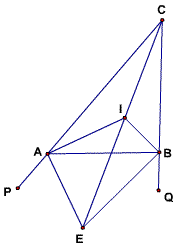
\includegraphics[scale=0.6]{xyz4Rr}
\end{center}
% https://s3.amazonaws.com/classroom.artofproblemsolving.com/Classes/GeomOlympiad/Images/xyz4Rr.gif


(In the below, $a$, $b$, $c$ are the usual $a = BC$, $b = AC$, $c = AB$)


    \begin{enumerate}
        \item Show that $AIC \sim EBC$ and $BIC \sim EAC$.
        
        
        \item Prove$$[EACB] = \dfrac{bxy}{2z} + \dfrac {br}2 + \dfrac {a^2br}{2z^2} = \dfrac{ axy}{2z} + \dfrac {ar}2 + \dfrac {b^2ar}{2z^2}$$
        
        
        \item Show that:$$ab - z^2 = \dfrac {xyz}r.$$
        
        
        \item Prove that:$$ \dfrac {ab - z^2}2 \cdot \sin C = rc. $$
    \end{enumerate}
\end{sketch}

\begin{mdsoln}
    \ \\
    \textbf{Solution 1} outline (the solution suggested by the hints, but much longer than the other solutions below!):
Extend $CI$ to the point $E$ such that $AE$ and $BE$ are exterior angle bisectors of $ABC$. Set $a = BC$, $b = CA$, $c = AB$.

Since $\angle EAI = 180^\circ - \angle IBE = 90^\circ$, $AEBI$ is cyclic, so
\[
\angle BEC = \angle BEI = \angle BAI = \angle IAC
\]Since we also have $\angle ECB = \angle ACI$, we can conclude that $\triangle BEC\sim \triangle IAC$. Likewise, $\triangle AEC\sim \triangle IBC$.

From $\triangle BEC\sim \triangle IAC$, we get
\[
[BEC] = [IAC]\left(\frac {BC}{IC}\right)^2 = \frac {1}{2}br\left(\frac {a}{z}\right)^2 = \frac {a^2br}{2z^2}
\]From $\triangle AEC\sim \triangle IBC$, we get
\[
AE = \frac {IB\cdot AC}{IC} = \frac {yb}{z}
\]Hence, the area of right triangle $IAE$ is
\[
\frac {1}{2}IA\cdot AE = \frac {bxy}{2z}
\]Therefore,
\[
[AEBC] = [IAE] + [IAC] + [BEC] = \frac {bxy}{2z} + \frac {br}{2} + \frac {a^2br}{2z^2}
\]Likewise,
\[
[AEBC] = \frac {axy}{2z} + \frac {ar}{2} + \frac {b^2ar}{2z^2}
\]Subtracting these two expressions yields
\[
0 = \frac {(b - a)xy}{2z} + \frac {(b - a)r}{2} - \frac {(b - a)abr}{2z^2}
\]Multiplying by $\frac {2z^2}{r(b - a)}$ gives us
\begin{eqnarray}0 & = & \frac {xyz}{r} + z^2 - ab\end{eqnarray}

\begin{lemma}
    $ab - z^2 = 2rc/\sin C$.
\end{lemma}
\begin{proof}
    Let $P,Q,R$ be the feet of the altitudes from $I$ to $BC,CA,AB$, respectively. Then, it is easy to see that $rc = [IQABP]$.
\end{proof} 

Now observe that
\begin{eqnarray*}\frac {z^2\sin C}{2} & = & z(z\cos (C/2))\sin C/2 \\
& = & (IC)(QC)\sin \angle QCI \\
& = & [IQCP]\end{eqnarray*}Hence,
\begin{eqnarray*}rc & = & [IQABP] \\
& = & [ABC] - [IQCP] \\
& = & \frac {ab\sin C}{2} - \frac {z^2\sin C}{2}\end{eqnarray*}from which the Lemma follows.
\vspace{6pt}

Now, substituting the expression from the Lemma into equation (1) yields
\[
0 = \frac {xyz}{r} - \frac {2rc}{\sin C}
\]implying that
\[
xyz = 2r^2\left(\frac {c}{\sin C}\right) = 2r^2(2R) = 4Rr^2
\]finally finishing the proof.

\vspace{10pt}
\textbf{Solution 2} outline (by Valentin Vornicu):
We can easily show using the Bisector Theorem that $AI = \dfrac {b + c}{a + b + c} w_a$, where $w_a$ is the length of the internal angle bisector from $A$. The relation becomes
\[
w_a w_b w_c (b + c)(c + a)(a + b) = 4Rr^2 \cdot 8s^3 .
\]But $rs = S$, so
\[
w_a w_b w_c (b + c)(c + a)(a + b) = 32 R S^2 s.
\]We also know that $4RS = abc$, and $w_a = \dfrac {2bc}{b + c} \cos \dfrac A2$, so
\[
8a^2b^2c^2 \cos \dfrac A2 \cos \dfrac B2 \cos \dfrac C2 = 8 abc Ss
\]so we only have to prove that
\[
abc \cos \dfrac A2 \cos \dfrac B2 \cos \dfrac C2 = Ss
\]But we know that $\cos \dfrac A2 = \sqrt {\dfrac {s(s - a)}{bc} }$, so the equality becomes
\[
\sqrt { s(s - a)(s - b)(s - c) } = S
\]which is as we all know the famous Heron's formula.

\vspace{10pt}

\textbf{Solution 3} outline:
Observe that the area of triangle $[BIC]$ is
\[
\frac {1}{2}yz\sin \angle BIC = \frac {1}{2}ar
\]Since $\angle BIC = 90^\circ + A/2$, this means that $\cos (A/2) = \frac {ar}{yz}$ so
\begin{align*}[ABC] & =  bc\sin(A/2)\cos(A/2) \\
& =  \frac {abcr\sin(A/2)}{yz}\end{align*}Then, $\frac {abc}{4R}  =  \frac {abcr\sin(A/2)}{yz}$, so
\[
4Rr^2 = \left(\frac {r}{\sin(A/2)}\right)yz = xyz
\]as desired.

\end{mdsoln}



\chapter{Construction}

\section{Session Transcript}
%------------------
%-- Message Achilleas ( moderator )
Today we will tackle a few more challenging construction problems. I stress constructions not because they are particularly common but because deeply understanding constructions leads to a deep understanding of basic Euclidean geometry.

%------------------
%-- Message Achilleas ( moderator )
We'll dive right into the problems.

%------------------
%-- Message Achilleas ( moderator )
\begin{example}
    Given a right triangle $ABC,$ construct a point $N$ inside the triangle such that angles $NBC,$ $NCA,$ and $NAB$ are equal.    
\end{example}

%------------------
%-- Message Achilleas ( moderator )
Where should we start?

%------------------
%-- Message MathJams ( user )
% draw a diagram so we have an idea where N is

%------------------
%-- Message mark888 ( user )
% Draw a diagram!

%------------------
%-- Message MeepMurp5 ( user )
% finished diagram?

%------------------
%-- Message Trollface60 ( user )
% draw a completed construction

%------------------
%-- Message chardikala2 ( user )
% start from the end?

%------------------
%-- Message dxs2016 ( user )
% diagram

%------------------
%-- Message coolbluealan ( user )
% diagram

%------------------
%-- Message pritiks ( user )
% draw a diagram

%------------------
%-- Message Achilleas ( moderator )
We start by sketching the 'finished' figure and looking for some information, or some way to relate what we want $(N)$ to what we have $(ABC).$

%------------------
%-- Message Achilleas ( moderator )
Are we going to chase lengths or angles?

%------------------
%-- Message Ezraft ( user )
% angles

%------------------
%-- Message mark888 ( user )
% Angles

%------------------
%-- Message Trollface60 ( user )
% angles

%------------------
%-- Message AOPS81619 ( user )
% The angles

%------------------
%-- Message JacobGallager1 ( user )
% Probably angles

%------------------
%-- Message Catherineyaya ( user )
% angles

%------------------
%-- Message coolbluealan ( user )
% angles

%------------------
%-- Message RP3.1415 ( user )
% angles probably

%------------------
%-- Message Wangminqi1 ( user )
% angles

%------------------
%-- Message TomQiu2023 ( user )
% angles

%------------------
%-- Message MathJams ( user )
% angle chase

%------------------
%-- Message Gamingfreddy ( user )
% angles

%------------------
%-- Message bigmath ( user )
% Angles

%------------------
%-- Message bryanguo ( user )
% angles

%------------------
%-- Message dxs2016 ( user )
% angles

%------------------
%-- Message laura.yingyue.zhang ( user )
% angles

%------------------
%-- Message Achilleas ( moderator )
Our 'finished' figure has a lot more information about angles than about lengths, so let's chase angles. With nothing obvious standing out we label a couple of angles and start chasing.

%------------------
%-- Message Achilleas ( moderator )



\begin{center}
\begin{asy}
import cse5;
import olympiad;
unitsize(4cm);

size(150);
pathpen = black + linewidth(0.7);
pointpen = black;
pen s = fontsize(8);
path scale(real s, pair D, pair E, real p) { return (point(D--E,p)+scale(s)*(-point(D--E,p)+D)--point(D--E,p)+scale(s)*(-point(D--E,p)+E));}
real tmp = 30;
pair B = dir(180-tmp), C = dir(180+tmp), A = dir(-tmp);
path circ = Circle((B+C)/2, length(B-C)/2);
pair X = IPs(C--(C+(B-A)),circ)[1];
pair N = IPs(A--X,circ)[0];
draw(MP("A",A,SE,s)--MP("B",B,rotate(180)*S,s)--MP("C",C,S,s)--cycle);
draw(N--A^^C--MP("N",N,NE,s)--B);
markscalefactor=0.025;
draw(anglemark(C,B,N)^^anglemark(B,A,N)^^anglemark(A,C,N));
draw(rightanglemark(B,C,A,2));
MP("x",A,rotate(-20)*scale(10)*W,s);
MP("x",C,rotate(10)*scale(10)*E,s);
MP("y",C,rotate(65)*scale(5)*E,s);
MP("x",B,rotate(10)*scale(10)*S,s);
MP("z",B,rotate(40)*scale(5)*S,s);
\end{asy}
\end{center}





%------------------
%-- Message Achilleas ( moderator )
Notice that we only stick in as many labels as we need. We don't need to label $\angle CAN$ because we can determine that in terms of the other labels we've placed already. Same goes for all the angles at $N.$

%------------------
%-- Message Achilleas ( moderator )
Can we make any observations?

%------------------
%-- Message bigmath ( user )
% x+y=90 degrees

%------------------
%-- Message MeepMurp5 ( user )
% $x+y = 90^{\circ}$

%------------------
%-- Message Catherineyaya ( user )
% $\angle BNC=90^\circ$

%------------------
%-- Message Wangminqi1 ( user )
% $y=90^{\circ}-x$

%------------------
%-- Message dxs2016 ( user )
% angle BNC = 90 degrees

%------------------
%-- Message MathJams ( user )
% $\angle BNC=90^{\circ}$

%------------------
%-- Message coolbluealan ( user )
% angle BNC seems to be a right angle

%------------------
%-- Message Lucky0123 ( user )
% $\triangle BNC$ looks like a right triangle

%------------------
%-- Message MeepMurp5 ( user )
% $\angle BNC = 90^{\circ}$

%------------------
%-- Message leoouyang ( user )
% Angle BNC is 90 degrees

%------------------
%-- Message Achilleas ( moderator )
The right angle at $C$ gives us $x + y = 90^\circ.$ How does this help?

%------------------
%-- Message pritiks ( user )
% angle BNC is 90 degrees

%------------------
%-- Message MathJams ( user )
% it gives us right angle $BNC$

%------------------
%-- Message TomQiu2023 ( user )
% $\angle CNB = 90$ degrees

%------------------
%-- Message Lucky0123 ( user )
% We can apply this to $\triangle BNC$ to get that $\angle BNC = 90^\circ$

%------------------
%-- Message JacobGallager1 ( user )
% This gives us that $\angle BNC= 90^\circ$.

%------------------
%-- Message Trollface60 ( user )
% angle BNC is right

%------------------
%-- Message Achilleas ( moderator )
This tells us that $\angle BNC$ is a right angle. That's useful information. Why does that help us find $N?$

%------------------
%-- Message coolbluealan ( user )
% N is on the circle with diameter BC

%------------------
%-- Message MathJams ( user )
% N lies on a semicircle with center of the midpoint of BC

%------------------
%-- Message ca981 ( user )
% Using BC as diameter, draw circle

%------------------
%-- Message JacobGallager1 ( user )
% It must be on the circle with diameter $BC$

%------------------
%-- Message AOPS81619 ( user )
% draw circle with diameter $BC$

%------------------
%-- Message Wangminqi1 ( user )
% it is on the circle with diameter $BC$

%------------------
%-- Message bryanguo ( user )
% $N$ lies on the circle with diameter $AC$

%------------------
%-- Message smileapple ( user )
% $N$ is on the semicircle with diameter $BC$

%------------------
%-- Message Catherineyaya ( user )
% N is on circle with diameter BC

%------------------
%-- Message vsar0406 ( user )
% Because we know that the circumcircle of BNC has diameter BC

%------------------
%-- Message Achilleas ( moderator )
Since $BNC$ is a right angle, point $N$ is on the circle with diameter $BC.$

%------------------
%-- Message Achilleas ( moderator )
This is very important - if you are hunting for a point and find that this point is the vertex of a right angle of a right triangle where the other two vertices are fixed, you know that the point is on the circle with the hypotenuse as diameter. Why does it make us happy to learn that our point is on a circle we can construct?

%------------------
%-- Message AOPS81619 ( user )
% It's the intersection of the circle and something else

%------------------
%-- Message MathJams ( user )
% we can maybe find an intersection, so that we can find the exact point

%------------------
%-- Message Ezraft ( user )
% it allows us to eventually construct the point by drawing the intersection of something and the circle

%------------------
%-- Message sae123 ( user )
% now we just need one more line or circle its on

%------------------
%-- Message Achilleas ( moderator )
Once we've found that our point is on a circle we can construct, all we have to do is show that the point is also on some line or circle or whatever, and we can locate the point at the intersection of our original circle and the line/circle/whatever.

%------------------
%-- Message Achilleas ( moderator )
We draw our circle and then look for more.

%------------------
%-- Message Achilleas ( moderator )



\begin{center}
\begin{asy}
import cse5;
import olympiad;
unitsize(4cm);

size(200);
pathpen = black + linewidth(0.7);
pointpen = black;
pen s = fontsize(8);
path scale(real s, pair D, pair E, real p) { return (point(D--E,p)+scale(s)*(-point(D--E,p)+D)--point(D--E,p)+scale(s)*(-point(D--E,p)+E));}
real tmp = 30;
pair B = dir(180-tmp), C = dir(180+tmp), A = dir(-tmp);
path circ = Circle((B+C)/2, length(B-C)/2);
pair X = IPs(C--(C+(B-A)),circ)[1];
pair N = IPs(A--X,circ)[0];
draw(circ,heavygreen);
draw(MP("A",A,SE,s)--MP("B",B,rotate(180)*S,s)--MP("C",C,S,s)--cycle);
draw(N--A^^C--MP("N",N,NE,s)--B);
markscalefactor=0.025;
draw(anglemark(C,B,N)^^anglemark(B,A,N)^^anglemark(A,C,N));
draw(rightanglemark(B,N,C,2)^^rightanglemark(B,C,A,2));
\end{asy}
\end{center}





%------------------
%-- Message Achilleas ( moderator )
Chasing angles with what we have so far doesn't appear too helpful.

%------------------
%-- Message TomQiu2023 ( user )
% $AC$ is also tangent to the circle

%------------------
%-- Message MathJams ( user )
% AC is tangent to our circle

%------------------
%-- Message Achilleas ( moderator )
Right. It is true that $\overline{AC}$ is tangent to the circle.

%------------------
%-- Message dxs2016 ( user )
% connect a line?

%------------------
%-- Message Achilleas ( moderator )
Often we have to explore a little - add a few lines here or there. Are there any lines that might be useful?

%------------------
%-- Message JacobGallager1 ( user )
% $AN$ would be useful if we could construct it

%------------------
%-- Message sae123 ( user )
% extend AN towards BC?

%------------------
%-- Message chardikala2 ( user )
% extend BN to meet AC

%------------------
%-- Message SlurpBurp ( user )
% extend $BN$ to meet $CA$?

%------------------
%-- Message Riya_Tapas ( user )
% Extend $CN$?

%------------------
%-- Message laura.yingyue.zhang ( user )
% intersection of AB and the circle to N

%------------------
%-- Message pritiks ( user )
% extend BN?

%------------------
%-- Message Lucky0123 ( user )
% Extend $AN$ past $N?$

%------------------
%-- Message Achilleas ( moderator )
We might consider extending any of $AN$, $BN$, or $CN$. Do any of them give us anything interesting?

%------------------
%-- Message ca981 ( user )
% extend AN to BC

%------------------
%-- Message bryanguo ( user )
% $AN$ is interesting

%------------------
%-- Message Achilleas ( moderator )
Extending $AN$ seems to be the most promising. Why?

%------------------
%-- Message MathJams ( user )
% it makes use of the circle (cyclic quadrilateral)

%------------------
%-- Message Riya_Tapas ( user )
% It intersects the diameter of the circle we constructed, most relevant

%------------------
%-- Message JacobGallager1 ( user )
% It intersects the green circle at $N$

%------------------
%-- Message Achilleas ( moderator )



\begin{center}
\begin{asy}
import cse5;
import olympiad;
unitsize(4cm);

size(200);
pathpen = black + linewidth(0.7);
pointpen = black;
pen s = fontsize(8);
path scale(real s, pair D, pair E, real p) { return (point(D--E,p)+scale(s)*(-point(D--E,p)+D)--point(D--E,p)+scale(s)*(-point(D--E,p)+E));}
real tmp = 30;
pair B = dir(180-tmp), C = dir(180+tmp), A = dir(-tmp);
path circ = Circle((B+C)/2, length(B-C)/2);
pair X = IPs(C--(C+(B-A)),circ)[1];
pair N = IPs(A--X,circ)[0];
pair Y = IPs(A--X,B--C)[0];
draw(circ,heavygreen);
draw(MP("A",A,SE,s)--MP("B",B,rotate(180)*S,s)--MP("C",C,S,s)--cycle);
draw(MP("X",X,SW,s)--A^^C--MP("N",N,NE,s)--B);
MP("Y",Y,NE,s);
markscalefactor=0.025;
draw(anglemark(C,B,N)^^anglemark(B,A,X)^^anglemark(A,C,N));
draw(rightanglemark(B,N,C,2)^^rightanglemark(B,C,A,2));
\end{asy}
\end{center}





%------------------
%-- Message Achilleas ( moderator )
It is promising as we can hit both $BC$ and the circle with it.

%------------------
%-- Message Achilleas ( moderator )
Does it help?

%------------------
%-- Message MeepMurp5 ( user )
% $XC \parallel AB$

%------------------
%-- Message Achilleas ( moderator )
Why?

%------------------
%-- Message Catherineyaya ( user )
% $\angle NAB=\angle NBC=\angle NXC,$ so $AB\parallel CX$

%------------------
%-- Message MathJams ( user )
% since $\angle AXC=\angle BAX$

%------------------
%-- Message Wangminqi1 ( user )
% $\angle CXN=\angle XAB$

%------------------
%-- Message SlurpBurp ( user )
% $\angle YXC = \angle YAB$

%------------------
%-- Message coolbluealan ( user )
% $\angle AXC=\angle CBN=\angle XAB$

%------------------
%-- Message ca981 ( user )
% angle CXN=angle CBN= angle XAB

%------------------
%-- Message laura.yingyue.zhang ( user )
% angle CXA is equal to angle CBN and thus angle NAB

%------------------
%-- Message SmartZX ( user )
% Angle CXN = Angle CBN = Angle XAB

%------------------
%-- Message Achilleas ( moderator )
We connect our $X$ to $B$ and $C$ and see that $\angle CXN = \angle CBN$ since they are inscribed in the same arc.

%------------------
%-- Message Achilleas ( moderator )



\begin{center}
\begin{asy}
import cse5;
import olympiad;
unitsize(4cm);

size(200);
pathpen = black + linewidth(0.7);
pointpen = black;
pen s = fontsize(8);
path scale(real s, pair D, pair E, real p) { return (point(D--E,p)+scale(s)*(-point(D--E,p)+D)--point(D--E,p)+scale(s)*(-point(D--E,p)+E));}
real tmp = 30;
pair B = dir(180-tmp), C = dir(180+tmp), A = dir(-tmp);
path circ = Circle((B+C)/2, length(B-C)/2);
pair X = IPs(C--(C+(B-A)),circ)[1];
pair N = IPs(A--X,circ)[0];
pair Y = IPs(A--X,B--C)[0];
draw(circ,heavygreen);
draw(MP("A",A,SE,s)--MP("B",B,rotate(180)*S,s)--MP("C",C,S,s)--cycle);
draw(C--MP("X",X,SW,s)--A^^C--MP("N",N,NE,s)--B--X);
MP("Y",Y,NE,s);
markscalefactor=0.025;
draw(anglemark(C,B,N)^^anglemark(B,A,X)^^anglemark(A,C,N)^^anglemark(C,X,A));
draw(rightanglemark(B,N,C,2)^^rightanglemark(B,C,A,2));
\end{asy}
\end{center}





%------------------
%-- Message Achilleas ( moderator )
Are we home?

%------------------
%-- Message MathJams ( user )
% yep!

%------------------
%-- Message MeepMurp5 ( user )
% yee

%------------------
%-- Message AOPS81619 ( user )
% Yes

%------------------
%-- Message Yufanwang ( user )
% yes

%------------------
%-- Message Lucky0123 ( user )
% yes

%------------------
%-- Message ca981 ( user )
% Yes!

%------------------
%-- Message Achilleas ( moderator )
We're home - our equal angles tell us that $CX$ and $AB$ are parallel. (This is why we mark equal angles as we go - so we can see cyclic quadrilaterals easily or parallel lines or similar triangles, etc.)  How does this lead to our construction?

%------------------
%-- Message Achilleas ( moderator )
You need to describe the steps carefully.

%------------------
%-- Message sae123 ( user )
% construct the circle with diameter $BC.$ Then construct $X$ so that $CX$ is parallel to $BA.$ Then $N$ is the other intersection of $XA$ with the circle.

%------------------
%-- Message laura.yingyue.zhang ( user )
% we construct the point X on the circle with diameter BC such that CX is parallel to AB. the intersection of AX and the circle with diameter BC is N

%------------------
%-- Message MathJams ( user )
% Construct our circle, then a line parallel to $AB$ through C, find the intersection of the circle and the line, label as X, then the intersection of XA nd the circle gives us N

%------------------
%-- Message SmartZX ( user )
% Construct a the circle with diameter BC, and draw a line through C parallel to AB. Let the point where this line intersects the circle other than C be X. Draw segment AX. The intersection of AX and the circle other than X is point N.

%------------------
%-- Message SlurpBurp ( user )
% construct a line parallel to $BA$ through $C$, name where the line meets the circle again $X$, $N$ is where $XA$ meets the circle again

%------------------
%-- Message coolbluealan ( user )
% We draw the circle with diameter BC, then draw the line through C parallel to AB. The line intersects the circle again at point X. N is the intersection of XA and the circle.

%------------------
%-- Message Catherineyaya ( user )
% construct circle with diameter BC (find center first), construct line through C parallel to AB intersecting the circle at a point X, AX intersects the circle at N

%------------------
%-- Message Ezraft ( user )
% first construct line $CX$ parallel to $AB$ through $C,$ then construct the circle with diameter $BC.$ Let $X$ be the intersection of this circle with $C.X$Then $N$ is the intersection between $AX$ and our circle. $\blacksquare$

%------------------
%-- Message Trollface60 ( user )
% construct a circle with diameter BC, then construct a line through C parallel to AB intersecting with the circle at X, connect AX, then mark N as the intersection of AX and the circle

%------------------
%-- Message Achilleas ( moderator )
We construct $N$ by constructing the circle with $BC$ as diameter. We then draw $CX$ parallel to $AB$ ($X$ is where this parallel hits the circle). We connect $A$ to $X$ and $N$ is the other intersection of $AX$ and our circle.

%------------------
%-- Message Achilleas ( moderator )
Are we finished with the problem?

%------------------
%-- Message MeepMurp5 ( user )
% no - we have to prove the construction works

%------------------
%-- Message Catherineyaya ( user )
% check the construction works

%------------------
%-- Message Riya_Tapas ( user )
% We have to show that the construction works

%------------------
%-- Message dxs2016 ( user )
% we need to prove that the construction represents our problem

%------------------
%-- Message coolbluealan ( user )
% We have to prove it works.

%------------------
%-- Message smileapple ( user )
% Prove it works!

%------------------
%-- Message JacobGallager1 ( user )
% No! We need to prove that the construction works

%------------------
%-- Message pritiks ( user )
% we have to prove the construction works

%------------------
%-- Message Achilleas ( moderator )
Not quite - we have to prove that our construction works. What exactly do we have to prove to show that our construction works?

%------------------
%-- Message TomQiu2023 ( user )
% we need to prove the three angles are equal

%------------------
%-- Message ay0741 ( user )
% you have to prove that the angles are congruent

%------------------
%-- Message MeepMurp5 ( user )
% that is, angles $NBC$, $NCA$, and  $NAB$ are equal.

%------------------
%-- Message Trollface60 ( user )
% angles NBC, NCA, and NAB are equal

%------------------
%-- Message MathJams ( user )
% show that our construction makes $\angle NBC=\angle NCA=\angle NAB$

%------------------
%-- Message vsar0406 ( user )
% that the angles NBC, NCA, and NAB are equal

%------------------
%-- Message Riya_Tapas ( user )
% We need to show that the specified angles are congruent when $N$ is constructed

%------------------
%-- Message Ezraft ( user )
% we have to prove that $\angle NBC = \angle NCA = \angle NAB$

%------------------
%-- Message Achilleas ( moderator )
We have to show that if we construct N as given above, that $\angle CBN = \angle BAN = \angle CAN$. How do we do it?

%------------------
%-- Message apple.xy ( user )
% angle chase?

%------------------
%-- Message TomQiu2023 ( user )
% Use our circle and the right angles that exist

%------------------
%-- Message Achilleas ( moderator )
We can basically work backwards from what we did before to find the construction. We start with angle $CXN $ and work from there - how?

%------------------
%-- Message Achilleas ( moderator )
(most of you show only one angle congruence)

%------------------
%-- Message TomQiu2023 ( user )
% $\angle CXN = \angle CBN = \angle NCA$ by tangent intersection theorem, also $\angle BAX = \angle AXC$ since our lines that we constructed are parallel, so the proof is done

%------------------
%-- Message ca981 ( user )
% ∠CXN=∠CBN (cyclic) =∠BAN (parallel) =∠NCA (tangent inscribed angle ∠NCA= ∠CBN)

%------------------
%-- Message chardikala2 ( user )
% angle CXN and CBN subtend the same arc so they are equal and since CX is parallel to AB, if we treat AX as a transversal through these two lines, then angle CXN and angle BAX are interior angles therefore they are equal

%------------------
%-- Message TomQiu2023 ( user )
% $\angle CXN = \angle CBN = \angle NCA$ by the tangent intersection theorem, $\angle BAX = \angle AXC$ since our lines $AB$ and $XC$ are parallel, and from the two above $\angle NBC = \angle NCA = \angle NAB$

%------------------
%-- Message coolbluealan ( user )
% We have $\angle NCA=\angle CXN$ because AC is tangent to the circle. We also have $\angle CXN=\angle XAB$ by parallel lines. $\angle CXN=\angle CBN$ from inscribed angles.

%------------------
%-- Message Wangminqi1 ( user )
% $\angle CXN=\angle CBN$ because they are equal inscribed angles, $\angle CXN=\angle NAB$ because of the parallel lines, and $\angle CXN=\angle NCA$ because $AC$ is a tangent line

%------------------
%-- Message mustwin_az ( user )
% $\angle CXN = \angle BAN$ since $CX \parallel AB $ and $\angle CXN = \angle CBN$ since $CNBX $ is cyclic

%------------------
%-- Message mark888 ( user )
% Because $\angle CXN$ shares arc $CN$ with $\angle NBC$, $\angle CXN=\angle NBC$. Because $\angle BCA$ is $90^{circ}$, $\angle NCA=\angle NBC$ also. Because $XC||BA$, $\angle CXN=\angle NAB$. Thus, $\angle NBC=\angle NCA=\angle NAB=\angle CXA$.

%------------------
%-- Message mark888 ( user )
% Because $\angle CXN$ shares arc $CN$ with $\angle NBC$, $\angle CXN=\angle NBC$. Because $\angle BCA$ is $90^{\circ}$, $\angle NCA=\angle NBC$ also. Because $XC||BA$, $\angle CXN=\angle NAB$. Thus, $\angle NBC=\angle NCA=\angle NAB=\angle CXA$.

%------------------
%-- Message AOPS81619 ( user )
% $\angle CXN=\angle XAB$ because of parallel lines, and $\angle CXN=\angle CBN$ because of cyclic quads


$\angle NCB=90-\angle CBN$, so $\angle NCA=90-\angle NCB=\angle NBC$

%------------------
%-- Message xyab ( user )
% $\angle CXN = \angle CBN$ because they intercept the same arc. $\angle CXN$ = $\angle BAX$ because we have parallel lines. $\angle CXN = \angle CAN$ by alternate segment theorem. thus all three angles are the same

%------------------
%-- Message vsar0406 ( user )
% Well, we know that because lines XC and AB are parallel, angle CXN = angle NAB. And then, because line AC is tangent to the circle at C, by the tangent chord theorem, we also have that angle ACN = angle CBN = angle CXN, so that shows that angles NBC, NCA, and NAB are equal.

%------------------
%-- Message Achilleas ( moderator )
$\angle BAN = \angle CXN$ due to parallel lines $AB$ and $CX.$

%------------------
%-- Message Achilleas ( moderator )
$\angle NBC$ is inscribed in the same arc as $\angle CXN$, so $\angle NBC = \angle CXN$.

%------------------
%-- Message Achilleas ( moderator )
Finally, $\angle ACN = \angle CBN$ because $\angle CNB$ is right (inscribed in a semicircle) and $\angle ACB$ is right, so both $\angle CBN$ and $\angle ACN$ are complementary to angle $\angle NCB$. Now we're finished.

%------------------
%-- Message Achilleas ( moderator )
You may wonder if we can construct, in an arbitrary triangle $ABC$, a point $N$ for which the angles $NBC$, $NCA$, and $NAB$ are equal.

%------------------
%-- Message Achilleas ( moderator )
The answer is...

%------------------
%-- Message tigerzhang ( user )
% yes?

%------------------
%-- Message RP3.1415 ( user )
% yes

%------------------
%-- Message mark888 ( user )
% Yes!

%------------------
%-- Message Yufanwang ( user )
% yes?

%------------------
%-- Message Achilleas ( moderator )
Yes! Here is a quick general construction. Form a circle through points $A$ and $B$, tangent to edge $BC$ of the triangle (think about how you can construct it).

%------------------
%-- Message Achilleas ( moderator )
Symmetrically, form a circle through points $B$ and $C$, tangent to edge $AC$, and a circle through points $A$ and $C$, tangent to edge $AB$. These three circles have a common point $N$, called the first Brocard point of the triangle $ABC$.

%------------------
%-- Message xyab ( user )
% are we going to do it?

%------------------
%-- Message Achilleas ( moderator )
You are welcome to do it on the message board after class. 

%------------------
%-- Message chardikala2 ( user )
% we don't have enough time unfortunately (totally guessing rn)

%------------------
%-- Message Achilleas ( moderator )
 Try to go through the details of this proof after class. By the way, the point $N$ is called the first Brocard point because there is a second Brocard point: the point $M$ such that the angles $MCB$, $MAC$ and $MBA$ are equal.

%------------------
%-- Message Achilleas ( moderator )
\vspace{10pt}
Next up:

%------------------
%-- Message Achilleas ( moderator )
\begin{example}
    Construct a right triangle $ABC$ with a given hypotenuse $c$ such that two of its medians are perpendicular.    
\end{example}

%------------------
%-- Message Achilleas ( moderator )
I'm guessing you know where we'll start with this one - working backwards and seeing what we can find.

%------------------
%-- Message Achilleas ( moderator )
Here's our 'finished' diagram.

%------------------
%-- Message Achilleas ( moderator )



\begin{center}
\begin{asy}
import cse5;
import olympiad;
unitsize(4cm);

size(150);
pathpen = black + linewidth(0.7);
pointpen = black;
pen s = fontsize(8);
path scale(real s, pair D, pair E, real p) { return (point(D--E,p)+scale(s)*(-point(D--E,p)+D)--point(D--E,p)+scale(s)*(-point(D--E,p)+E));}
pair A = dir(180), M = origin, B = dir(0);
pair N = IPs(Circle((-.25,0),0.75), Circle((0.5,0),0.5))[0];
pair C = IPs(Circle((0,0),1),scale(2,B,N,0))[1];
pair G = extension(A,N,C,M);

//draw(Circle((0,0),1),heavygreen);
//draw(Circle((-0.5,0),0.5),heavygreen);
//draw(Circle((0.5,0),0.5),heavygreen);
//draw(Circle((-.25,0),0.75),heavygreen);

draw(MP("A",A,W,s)--MP("M",M,SE,s)--MP("B",B,E,s));
draw(A--MP("C",C,NW,s)--M^^C--B^^A--MP("N",N,NE,s));
MP("G",G,scale(2)*dir(60),s);

draw(rightanglemark(A,C,B,2.5)^^rightanglemark(A,G,C,2.5));
\end{asy}
\end{center}





%------------------
%-- Message Achilleas ( moderator )
How do we know that medians $AN$ and $BP$ aren't perpendicular?

%------------------
%-- Message pritiks ( user )
% what is P?

%------------------
%-- Message mark888 ( user )
% Where is P?

%------------------
%-- Message Achilleas ( moderator )
$P$ is somewhere on $AC$, while $BP$ is the median from $B$.

%------------------
%-- Message Gamingfreddy ( user )
% because angle AGB must be obtuse.

%------------------
%-- Message Achilleas ( moderator )
Because $\angle AGB$ is obtuse.

%------------------
%-- Message Achilleas ( moderator )
The first step of the construction is easy. What is it?

%------------------
%-- Message razmath ( user )
% construct AB?

%------------------
%-- Message Achilleas ( moderator )
We are given hypotenuse $c$, so we can construct a segment $AB$ of length $c$.

%------------------
%-- Message Achilleas ( moderator )
What can we say about point $C?$

%------------------
%-- Message MeepMurp5 ( user )
% we know $C$ lies on the circle with diameter $AB$, assuming that $AB=c$

%------------------
%-- Message MathJams ( user )
% lies on a circle with diameter AB

%------------------
%-- Message razmath ( user )
% its on the circle with diameter AB

%------------------
%-- Message Ezraft ( user )
% $C$ is on the circle with diameter $AB$

%------------------
%-- Message Trollface60 ( user )
% C is on the circle with diameter AB

%------------------
%-- Message dxs2016 ( user )
% on the circle formed by diameter AB

%------------------
%-- Message Catherineyaya ( user )
% C is on the circle with diameter AB

%------------------
%-- Message Gamingfreddy ( user )
% C is on the circle with diameter AB.

%------------------
%-- Message coolbluealan ( user )
% it is on the circle with diameter AB

%------------------
%-- Message AOPS81619 ( user )
% It's on the circle with diameter $AB$

%------------------
%-- Message SlurpBurp ( user )
% it lies on the circle that has $AB$ as a diameter

%------------------
%-- Message ay0741 ( user )
% its on the circle with diameter AB

%------------------
%-- Message Trollyjones ( user )
% it lies on the circle we can construct with diameter AB

%------------------
%-- Message trk08 ( user )
% on the circle where the diameter is c

%------------------
%-- Message christopherfu66 ( user )
% it is on a circle with diameter AB

%------------------
%-- Message RP3.1415 ( user )
% C lies on the circle with diameter $AB$

%------------------
%-- Message ca981 ( user )
% On circle with AB as diameter

%------------------
%-- Message ww2511 ( user )
% must lie on the circle with diameter AB

%------------------
%-- Message mustwin_az ( user )
% its on the cirlce with diameter AB

%------------------
%-- Message sae123 ( user )
% C lies on the circle with a diameter of $AB$

%------------------
%-- Message Achilleas ( moderator )
$C$ lives on the circle with diameter $AB$.

%------------------
%-- Message Achilleas ( moderator )



\begin{center}
\begin{asy}
import cse5;
import olympiad;
unitsize(4cm);

size(150);
pathpen = black + linewidth(0.7);
pointpen = black;
pen s = fontsize(8);
path scale(real s, pair D, pair E, real p) { return (point(D--E,p)+scale(s)*(-point(D--E,p)+D)--point(D--E,p)+scale(s)*(-point(D--E,p)+E));}
pair A = dir(180), M = origin, B = dir(0);
pair N = IPs(Circle((-.25,0),0.75), Circle((0.5,0),0.5))[0];
pair C = IPs(Circle((0,0),1),scale(2,B,N,0))[1];
pair G = extension(A,N,C,M);

draw(Circle((0,0),1),heavygreen);
//draw(Circle((-0.5,0),0.5),heavygreen);
//draw(Circle((0.5,0),0.5),heavygreen);
//draw(Circle((-.25,0),0.75),heavygreen);

draw(MP("A",A,W,s)--MP("M",M,SE,s)--MP("B",B,E,s));
draw(A--MP("C",C,NW,s)--M^^C--B^^A--MP("N",N,NE,s));
MP("G",G,scale(2)*dir(60),s);

draw(rightanglemark(A,C,B,2.5)^^rightanglemark(A,G,C,2.5));
\end{asy}
\end{center}





%------------------
%-- Message Achilleas ( moderator )
We don't see how to construct $C$ directly. Can we get any more information about any of the other points in our diagram?

%------------------
%-- Message MathJams ( user )
% $M$ is the center of the circle

%------------------
%-- Message ww2511 ( user )
% M is the center of the circle

%------------------
%-- Message RP3.1415 ( user )
% M is the center of this circle

%------------------
%-- Message mustwin_az ( user )
% M is the center of the circle

%------------------
%-- Message sae123 ( user )
% $M$ is the midpoint of $AB$

%------------------
%-- Message Lucky0123 ( user )
% $M$ is the center of the circle with diameter $AB$

%------------------
%-- Message Achilleas ( moderator )
We can easily construct $M$. Since angle $AGM$ is a right angle, $G$ lives on the circle with diameter $AM$ (which we can construct).

%------------------
%-- Message Achilleas ( moderator )



\begin{center}
\begin{asy}
import cse5;
import olympiad;
unitsize(4cm);

size(150);
pathpen = black + linewidth(0.7);
pointpen = black;
pen s = fontsize(8);
path scale(real s, pair D, pair E, real p) { return (point(D--E,p)+scale(s)*(-point(D--E,p)+D)--point(D--E,p)+scale(s)*(-point(D--E,p)+E));}
pair A = dir(180), M = origin, B = dir(0);
pair N = IPs(Circle((-.25,0),0.75), Circle((0.5,0),0.5))[0];
pair C = IPs(Circle((0,0),1),scale(2,B,N,0))[1];
pair G = extension(A,N,C,M);

draw(Circle((0,0),1),heavygreen);
draw(Circle((-0.5,0),0.5),heavygreen);
//draw(Circle((0.5,0),0.5),heavygreen);
//draw(Circle((-.25,0),0.75),heavygreen);

draw(MP("A",A,W,s)--MP("M",M,SE,s)--MP("B",B,E,s));
draw(A--MP("C",C,NW,s)--M^^C--B^^A--MP("N",N,NE,s));
MP("G",G,scale(2)*dir(60),s);

draw(rightanglemark(A,C,B,2.5)^^rightanglemark(A,G,C,2.5));
\end{asy}
\end{center}





%------------------
%-- Message Achilleas ( moderator )
It may look like we're done, but if we were working forwards building our circles, our diagram would look like this:

%------------------
%-- Message Achilleas ( moderator )



\begin{center}
\begin{asy}
import cse5;
import olympiad;
unitsize(4cm);

size(150);
pathpen = black + linewidth(0.7);
pointpen = black;
pen s = fontsize(8);
path scale(real s, pair D, pair E, real p) { return (point(D--E,p)+scale(s)*(-point(D--E,p)+D)--point(D--E,p)+scale(s)*(-point(D--E,p)+E));}
pair A = (-1,0), M = (0,0), B = (1,0);
draw(Circle((0,0),1),heavygreen);
draw(Circle((-0.5,0),0.5),heavygreen);
draw(MP("A",A,W,s)--MP("M",M,SE,s)--MP("B",B,E,s));
\end{asy}
\end{center}





%------------------
%-- Message xyab ( user )
% lol

%------------------
%-- Message Achilleas ( moderator )
(Have to keep an eye on both of these diagrams as we go - going forwards and backwards. It's easy to confuse them and think you're finished when you're not.)

%------------------
%-- Message Achilleas ( moderator )
So now what?

%------------------
%-- Message Achilleas ( moderator )
Are there any more circles or lines to draw?

%------------------
%-- Message Achilleas ( moderator )
We've drawn a circle for $G$, and for $C$. Can we draw one for $N?$

%------------------
%-- Message Achilleas ( moderator )
We can draw one for $N$. What circle can we draw for $N?$

%------------------
%-- Message coolbluealan ( user )
% N is on the circle with diameter MB

%------------------
%-- Message myltbc10 ( user )
% circle with diameter MB

%------------------
%-- Message AOPS81619 ( user )
% Oh the circle with diameter $MB$

%------------------
%-- Message MeepMurp5 ( user )
% circle with diameter $BM$

%------------------
%-- Message sae123 ( user )
% with diameter MB

%------------------
%-- Message tigerzhang ( user )
% Circle with diameter BM

%------------------
%-- Message Achilleas ( moderator )
Point $N$ must be on the circle with $BM$ as a diameter. Why?

%------------------
%-- Message AOPS81619 ( user )
% $MN$ is parallel to $AC$?

%------------------
%-- Message Achilleas ( moderator )
Yes, it is. Why?

%------------------
%-- Message dxs2016 ( user )
% M is midpoint of AB, N is midpoint of BC, MN is midsegment and is parallel to AC

%------------------
%-- Message Gamingfreddy ( user )
% Since M and N are midpoints of AB and BC respectively

%------------------
%-- Message bigmath ( user )
% it's one of the sides of the medial triangle

%------------------
%-- Message sae123 ( user )
% because MN is a side of the medial triangle

%------------------
%-- Message Achilleas ( moderator )
That's right! $M$ and $N$ are the midpoints of $\overline{AB}$ and $\overline{CB}$ respectively, so the midline theorem applies.

%------------------
%-- Message SlurpBurp ( user )
% there is a homothety with ratio 1/2 centered at $B$ that maps $MN$ to $AC$

%------------------
%-- Message AOPS81619 ( user )
% Because $M$ and $N$ are both medians, so we can uses SAS similarity

%------------------
%-- Message SmartZX ( user )
% Triangle MBN and Triangle ABC are homothetic through point B

%------------------
%-- Message christopherfu66 ( user )
% B is the center of homothety from triangle MNB to ACB

%------------------
%-- Message mustwin_az ( user )
% the circle with diameter MB is homothetic to circle with diameter AB with B as the center of homothety

%------------------
%-- Message Achilleas ( moderator )
The circle with $BM$ as diameter is homothetic to the large circle with center $B$ and ratio $1/2$, since diameter $BM$ is $1/2$ diameter $AB$ of the large circle. Hence, if we define point $N$ to be the point where the smaller circle meets $BC$, we see that $N$ is the midpoint of $BC$ as desired since $BN = BC/2$ due to our homothety.

%------------------
%-- Message Achilleas ( moderator )



\begin{center}
\begin{asy}
import cse5;
import olympiad;
unitsize(4cm);

size(150);
pathpen = black + linewidth(0.7);
pointpen = black;
pen s = fontsize(8);
path scale(real s, pair D, pair E, real p) { return (point(D--E,p)+scale(s)*(-point(D--E,p)+D)--point(D--E,p)+scale(s)*(-point(D--E,p)+E));}
pair A = dir(180), M = origin, B = dir(0);
pair N = IPs(Circle((-.25,0),0.75), Circle((0.5,0),0.5))[0];
pair C = IPs(Circle((0,0),1),scale(2,B,N,0))[1];
pair G = extension(A,N,C,M);

draw(Circle((0,0),1),heavygreen);
draw(Circle((-0.5,0),0.5),heavygreen);
draw(Circle((0.5,0),0.5),heavygreen);
//draw(Circle((-.25,0),0.75),heavygreen);

draw(MP("A",A,W,s)--MP("M",M,SE,s)--MP("B",B,E,s));
draw(A--MP("C",C,NW,s)--M^^C--B^^A--MP("N",N,NE,s));
MP("G",G,scale(2)*dir(60),s);

draw(rightanglemark(A,C,B,2.5)^^rightanglemark(A,G,C,2.5));
\end{asy}
\end{center}





%------------------
%-- Message Achilleas ( moderator )
We're still not finished. If we could find any of $G,$ $N,$ or $C,$ we'd be finished, but we only have a circle for each. We need another line or another circle.

%------------------
%-- Message Achilleas ( moderator )
One thing we might ask ourselves here is 'What information have I not used?'  (In general, this is extremely useful when stuck on a geometry problem. It's perhaps more useful on a geometry problem than any other type of problem.)

%------------------
%-- Message Achilleas ( moderator )
What information have we not used?

%------------------
%-- Message Achilleas ( moderator )
We've used the fact that $C$ is right, that $M$ is a midpoint, that $N$ is a midpoint, that $AGM$ is right. What haven't we used?

%------------------
%-- Message Ezraft ( user )
% $G$ is the centroid?

%------------------
%-- Message Achilleas ( moderator )
We haven't used the fact that $G$ is the centroid. What good does that do?

%------------------
%-- Message TomQiu2023 ( user )
% $CG = 2 GM$

%------------------
%-- Message bryanguo ( user )
% splits the medians into ratio $2:1$

%------------------
%-- Message Ezraft ( user )
% $AG = 2 \cdot GN$

%------------------
%-- Message apple.xy ( user )
% AG/GN = CG/GM = 2

%------------------
%-- Message bryanguo ( user )
% $AG:GN=2:1$ and $CG:GM=2:1$

%------------------
%-- Message mark888 ( user )
% All the medians are split into a ratio of 2:1

%------------------
%-- Message Lucky0123 ( user )
% It splits the medians in a 2:1 ratio

%------------------
%-- Message pritiks ( user )
% CG = 2GM

%------------------
%-- Message Achilleas ( moderator )
Since $G$ is a centroid, $AG = 2GN$ and $CG = 2GM.$ So?  How can we use this to finish the construction?

%------------------
%-- Message Achilleas ( moderator )
We've drawn plenty of circles - is there one more to draw?

%------------------
%-- Message Achilleas ( moderator )
I see that some of you say: the circle with diameter $AN$. This is trivially true and does not help us construct $N$.

%------------------
%-- Message Achilleas ( moderator )
We are looking for $N$ as the intersection of two circles. We have determined one of them and we need to use the properties of the centroid to find another circle.

%------------------
%-- Message Achilleas ( moderator )
Having used homothety to note that $N$ is on the circle with $BM$ as diameter since $BN/BC = BM/AB = 1/2$, we see ratios connected to another center of homothety candidate. Which one?

%------------------
%-- Message Achilleas ( moderator )
Note that $(AG/AN = 2/3)$ and that $N$ lives on the circle through $A$ with diameter $AK$ where $K$ is on $AB$ such that $AM/AK = 2/3$ (thus, the circle with diameter $AK$ is homothetic to the circle with diameter $AM$).

%------------------
%-- Message Achilleas ( moderator )
How do we find $K?$

%------------------
%-- Message MathJams ( user )
% Midpoint of MB

%------------------
%-- Message TomQiu2023 ( user )
% it's the midpoint of MB

%------------------
%-- Message Lucky0123 ( user )
% $K$ is the midpoint of $MB$

%------------------
%-- Message christopherfu66 ( user )
% K is the midpoint of BM.

%------------------
%-- Message Trollyjones ( user )
% the midpoint of MB

%------------------
%-- Message bryanguo ( user )
% looks like midpoint of $BM$

%------------------
%-- Message ca981 ( user )
% K is midpoint of BM

%------------------
%-- Message MeepMurp5 ( user )
% midpoint $MB$

%------------------
%-- Message ay0741 ( user )
% midpoint of MB

%------------------
%-- Message Riya_Tapas ( user )
% Take the midpoint of $BM$

%------------------
%-- Message Achilleas ( moderator )
$AK/AM = 3/2,$ so $K$ is just the midpoint of $BM.$ We locate $K$ as the midpoint of $BM$ and draw the circle to give us $N.$

%------------------
%-- Message Achilleas ( moderator )



\begin{center}
\begin{asy}
import cse5;
import olympiad;
unitsize(4cm);

size(150);
pathpen = black + linewidth(0.7);
pointpen = black;
pen s = fontsize(8);
path scale(real s, pair D, pair E, real p) { return (point(D--E,p)+scale(s)*(-point(D--E,p)+D)--point(D--E,p)+scale(s)*(-point(D--E,p)+E));}
pair A = dir(180), M = origin, B = dir(0);
pair N = IPs(Circle((-.25,0),0.75), Circle((0.5,0),0.5))[0];
pair C = IPs(Circle((0,0),1),scale(2,B,N,0))[1];
pair G = extension(A,N,C,M);

draw(Circle((0,0),1),heavygreen);
draw(Circle((-0.5,0),0.5),heavygreen);
draw(Circle((0.5,0),0.5),heavygreen);
draw(Circle((-.25,0),0.75),heavygreen);

draw(MP("A",A,W,s)--MP("M",M,SE,s)--MP("B",B,E,s));
draw(A--MP("C",C,NW,s)--M^^C--B^^A--MP("N",N,NE,s));
MP("G",G,scale(2)*dir(60),s);

draw(rightanglemark(A,C,B,2.5)^^rightanglemark(A,G,C,2.5));
\end{asy}
\end{center}





%------------------
%-- Message Achilleas ( moderator )
Going forwards, our construction now looks like this:

%------------------
%-- Message Achilleas ( moderator )



\begin{center}
\begin{asy}
import cse5;
import olympiad;
unitsize(4cm);

size(150);
pathpen = black + linewidth(0.7);
pointpen = black;
pen s = fontsize(8);
path scale(real s, pair D, pair E, real p) { return (point(D--E,p)+scale(s)*(-point(D--E,p)+D)--point(D--E,p)+scale(s)*(-point(D--E,p)+E));}
pair A = dir(180), M = origin, B = dir(0);
pair N = IPs(Circle((-.25,0),0.75), Circle((0.5,0),0.5))[0];
pair C = IPs(Circle((0,0),1),scale(2,B,N,0))[1];
pair G = extension(A,N,C,M);

draw(Circle((0,0),1),heavygreen);
draw(Circle((-0.5,0),0.5),heavygreen);
draw(Circle((0.5,0),0.5),heavygreen);
draw(Circle((-.25,0),0.75),heavygreen);

draw(MP("A",A,W,s)--MP("M",M,SE,s)--MP("B",B,E,s));
//draw(A--MP("C",C,NW,s)--M^^C--B^^A--MP("N",N,NE,s));
MP("N",N,NE,s);
//MP("G",G,scale(2)*dir(60),s);

//draw(rightanglemark(A,C,B,2.5)^^rightanglemark(A,G,C,2.5));
\end{asy}
\end{center}





%------------------
%-- Message Achilleas ( moderator )
Now how do we construct point $C?$

%------------------
%-- Message razmath ( user )
% extend BN to hit the largest circle at another point not equal to B

%------------------
%-- Message mark888 ( user )
% Extend BN to the large circle

%------------------
%-- Message SlurpBurp ( user )
% extend $NB$ to meet the largest circle again

%------------------
%-- Message MeepMurp5 ( user )
% the intersection of $NB$ and the circle with diameter $AB$ not equivalent to $B$

%------------------
%-- Message ww2511 ( user )
% extend BN beyond N

%------------------
%-- Message Lucky0123 ( user )
% Extend $BN$ past $N$ to hit the big circle

%------------------
%-- Message RP3.1415 ( user )
% draw $NB$ and intersect it with the big circle

%------------------
%-- Message pritiks ( user )
% extend BN to hit the circle

%------------------
%-- Message JacobGallager1 ( user )
% Extend $BN$ onto the big circle

%------------------
%-- Message christopherfu66 ( user )
% Draw line BN to intersect the circle with diameter AB at C.

%------------------
%-- Message Achilleas ( moderator )
We locate $C$ by extending $BN$ past $N.$ Where it hits the largest circle again is point $C.$

%------------------
%-- Message Achilleas ( moderator )
Where "large circle" is the circle with diameter $\overline{AB}$.

%------------------
%-- Message Achilleas ( moderator )
We can't say extend $\overline{BN}$ to meet the circumcircle of $ABC$ to obtain $C$ because it is the point $C$ that we want to construct.

%------------------
%-- Message Achilleas ( moderator )
I'll leave the proof that this construction works for the message board.

%------------------
%-- Message Achilleas ( moderator )
There are lots of other approaches to this problem, see if you can find them.

%------------------
%-- Message Achilleas ( moderator )
\vspace{10pt}
Next example:

%------------------
%-- Message Achilleas ( moderator )
\begin{example}
    $ABCD$ and $A'B'C'D'$ are square maps of the same region, drawn to different scales and superimposed as shown in the figure. There is only one point $O$ on the small map which lies directly over point $O'$ on the large map such that $O$ and $O'$ each represent the same place of the region. Give a Euclidean construction that produces this point.    
\end{example}


%------------------
%-- Message Achilleas ( moderator )



\begin{center}
\begin{asy}
import cse5;
import olympiad;
unitsize(4cm);

size(175);
pathpen = black + linewidth(0.7);
pointpen = black;
pen s = fontsize(8);
path scale(real s, pair D, pair E, real p) { return (point(D--E,p)+scale(s)*(-point(D--E,p)+D)--point(D--E,p)+scale(s)*(-point(D--E,p)+E));}
real rotate_factor = -70;
real scale_factor = 0.4;
pair shift_factor = (0.1,-0.07);
pair AA = dir(135), BB = dir(45), CC = dir(-45), DD = dir(-135);
pair A = shift_factor+scale(scale_factor)*rotate(rotate_factor)*AA, 
    B = shift_factor+scale(scale_factor)*rotate(rotate_factor)*BB, 
    C = shift_factor+scale(scale_factor)*rotate(rotate_factor)*CC, 
    D = shift_factor+scale(scale_factor)*rotate(rotate_factor)*DD;
draw(MP("A'",AA,NW,s)--MP("B'",BB,NE,s)--MP("C'",CC,SE,s)--MP("D'",DD,SW,s)--cycle);
draw(MP("A",A,NE,s)--MP("B",B,SE,s)--MP("C",C,SW,s)--MP("D",D,NW,s)--cycle);
\end{asy}
\end{center}





%------------------
%-- Message Achilleas ( moderator )
Hmmm…  Now what?

%------------------
%-- Message xyab ( user )
% find O from reverse?

%------------------
%-- Message Ezraft ( user )
% draw the 'finished' diagram

%------------------
%-- Message Achilleas ( moderator )
We go ahead with our usual working backwards approach:

%------------------
%-- Message Achilleas ( moderator )



\begin{center}
\begin{asy}
import cse5;
import olympiad;
unitsize(4cm);

size(200);
pathpen = black + linewidth(0.7);
pointpen = black;
pen s = fontsize(8);
path scale(real s, pair D, pair E, real p) { return (point(D--E,p)+scale(s)*(-point(D--E,p)+D)--point(D--E,p)+scale(s)*(-point(D--E,p)+E));}
real rotate_factor = -70;
real scale_factor = 0.4;
pair shift_factor = (0.1,-0.07);
pair AA = dir(135), BB = dir(45), CC = dir(-45), DD = dir(-135);
pair A = shift_factor+scale(scale_factor)*rotate(rotate_factor)*AA, 
    B = shift_factor+scale(scale_factor)*rotate(rotate_factor)*BB, 
    C = shift_factor+scale(scale_factor)*rotate(rotate_factor)*CC, 
    D = shift_factor+scale(scale_factor)*rotate(rotate_factor)*DD;

pair X = extension(AA,BB,A,B);
pair O = IPs(circumcircle(AA,X,A),circumcircle(BB,X,B))[1];
dot(MP("O",O,dir(200),s));
draw(MP("A'",AA,NW,s)--MP("B'",BB,NE,s)--MP("C'",CC,SE,s)--MP("D'",DD,SW,s)--cycle);
draw(MP("A",A,NE,s)--MP("B",B,SE,s)--MP("C",C,SW,s)--MP("D",D,NW,s)--cycle);
\end{asy}
\end{center}





%------------------
%-- Message Achilleas ( moderator )
Um. Looks like we'll need a little more. What should we add and why?

%------------------
%-- Message Achilleas ( moderator )
How can we tell if a point is our desired $O$ (i.e. the same site on both maps)?

%------------------
%-- Message TomQiu2023 ( user )
% Connect O to the vertices of the square

%------------------
%-- Message Achilleas ( moderator )
Which square?

%------------------
%-- Message MathJams ( user )
% both squares

%------------------
%-- Message Ezraft ( user )
% both squares

%------------------
%-- Message Achilleas ( moderator )
$O$ must be in the same position relative to the corners of each square.

%------------------
%-- Message Achilleas ( moderator )



\begin{center}
\begin{asy}
import cse5;
import olympiad;
unitsize(4cm);

size(200);
pathpen = black + linewidth(0.7);
pointpen = black;
pen s = fontsize(8);
path scale(real s, pair D, pair E, real p) { return (point(D--E,p)+scale(s)*(-point(D--E,p)+D)--point(D--E,p)+scale(s)*(-point(D--E,p)+E));}
real rotate_factor = -70;
real scale_factor = 0.4;
pair shift_factor = (0.1,-0.07);
pair AA = dir(135), BB = dir(45), CC = dir(-45), DD = dir(-135);
pair A = shift_factor+scale(scale_factor)*rotate(rotate_factor)*AA, 
    B = shift_factor+scale(scale_factor)*rotate(rotate_factor)*BB, 
    C = shift_factor+scale(scale_factor)*rotate(rotate_factor)*CC, 
    D = shift_factor+scale(scale_factor)*rotate(rotate_factor)*DD;

pair X = extension(AA,BB,A,B); 
//draw(MP("X",X,N,s)--A);
//draw(circumcircle(AA,X,A)^^circumcircle(BB,X,B),deepgreen);
pair O = IPs(circumcircle(AA,X,A),circumcircle(BB,X,B))[1];
draw(MP("O",O,dir(200),s)--A^^O--B^^O--C^^O--D,red);
draw(O--AA^^O--BB^^O--CC^^O--DD,green);
draw(MP("A'",AA,NW,s)--MP("B'",BB,NE,s)--MP("C'",CC,SE,s)--MP("D'",DD,SW,s)--cycle);
draw(MP("A",A,NE,s)--MP("B",B,SE,s)--MP("C",C,SW,s)--MP("D",D,NW,s)--cycle);
draw(MP("x",O,scale(5)*N,s+green)^^
    MP("w",O,scale(5)*W,s+green)^^
    MP("y",O,scale(5)*E,s+green)^^
    MP("z",O,scale(5)*S,s+green));
draw(MP("x",O,rotate(rotate_factor)*scale(4)*N,s+mediumred)^^
    MP("w",O,rotate(rotate_factor)*scale(4)*W,s+mediumred)^^
    MP("y",O,rotate(rotate_factor)*scale(4)*E,s+mediumred)^^
    MP("z",O,rotate(rotate_factor)*scale(4)*S,s+mediumred));
\end{asy}
\end{center}





%------------------
%-- Message Achilleas ( moderator )
In the diagram, the lowercase colored letters are angle measures of the corresponding angles (green for the green angles, red for the red).

%------------------
%-- Message Achilleas ( moderator )
What now?

%------------------
%-- Message SmartZX ( user )
% Can we use homothety?

%------------------
%-- Message Achilleas ( moderator )
Homothety alone is hard to apply.

%------------------
%-- Message JacobGallager1 ( user )
% There aren't really any parallel segments

%------------------
%-- Message Achilleas ( moderator )
Are there other angles we know must be equal?

%------------------
%-- Message mustwin_az ( user )
% $\angle OA'B=\angle OAB$

%------------------
%-- Message JacobGallager1 ( user )
% $\angle OA'D' = \angle OAD$

%------------------
%-- Message ww2511 ( user )
% angles OAB and OA'B' etc

%------------------
%-- Message Ezraft ( user )
% $\angle OCB = \angle OC'B'$ as well as other similar angles

%------------------
%-- Message dxs2016 ( user )
% ex. angle ADO = angle A'D'O?

%------------------
%-- Message Trollyjones ( user )
% like angle DAO= angle D'A'O

%------------------
%-- Message Achilleas ( moderator )
The angles the red and green lines form with the sides of the square are equal:

%------------------
%-- Message Achilleas ( moderator )



\begin{center}
\begin{asy}
import cse5;
import olympiad;
unitsize(4cm);

size(200);
pathpen = black + linewidth(0.7);
pointpen = black;
pen s = fontsize(8);
path scale(real s, pair D, pair E, real p) { return (point(D--E,p)+scale(s)*(-point(D--E,p)+D)--point(D--E,p)+scale(s)*(-point(D--E,p)+E));}
real rotate_factor = -70;
real scale_factor = 0.4;
pair shift_factor = (0.1,-0.07);
pair AA = dir(135), BB = dir(45), CC = dir(-45), DD = dir(-135);
pair A = shift_factor+scale(scale_factor)*rotate(rotate_factor)*AA, 
    B = shift_factor+scale(scale_factor)*rotate(rotate_factor)*BB, 
    C = shift_factor+scale(scale_factor)*rotate(rotate_factor)*CC, 
    D = shift_factor+scale(scale_factor)*rotate(rotate_factor)*DD;

pair X = extension(AA,BB,A,B); 
//draw(MP("X",X,N,s)--A);
//draw(circumcircle(AA,X,A)^^circumcircle(BB,X,B),deepgreen);
pair O = IPs(circumcircle(AA,X,A),circumcircle(BB,X,B))[1];
draw(MP("O",O,dir(200),s)--A^^O--B^^O--C^^O--D,red);
draw(O--AA^^O--BB^^O--CC^^O--DD,green);
draw(MP("A'",AA,NW,s)--MP("B'",BB,NE,s)--MP("C'",CC,SE,s)--MP("D'",DD,SW,s)--cycle);
draw(MP("A",A,NE,s)--MP("B",B,SE,s)--MP("C",C,SW,s)--MP("D",D,NW,s)--cycle);
draw(MP("a",AA,scale(5)*ESE,s+green)^^
    MP("b",BB,scale(5)*WSW,s+green)^^
    MP("x",O,scale(5)*N,s+green)^^
    MP("w",O,scale(5)*W,s+green)^^
    MP("y",O,scale(5)*E,s+green)^^
    MP("z",O,scale(5)*S,s+green));
draw(MP("a",A,scale(5)*S,s+red)^^
    MP("b",B,scale(5)*NW,s+red)^^
    MP("x",O,rotate(rotate_factor)*scale(4)*N,s+mediumred)^^
    MP("w",O,rotate(rotate_factor)*scale(4)*W,s+mediumred)^^
    MP("y",O,rotate(rotate_factor)*scale(4)*E,s+mediumred)^^
    MP("z",O,rotate(rotate_factor)*scale(4)*S,s+mediumred));
\end{asy}
\end{center}





%------------------
%-- Message Achilleas ( moderator )
(I only marked a couple pairs of these angles - $a$ and $b$ in the diagram; clearly there are 6 more similar pairs.)

%------------------
%-- Message Achilleas ( moderator )
Now what?

%------------------
%-- Message dxs2016 ( user )
% similar triangles?

%------------------
%-- Message Achilleas ( moderator )
What's a triangle similar to $\triangle AOB ?$

%------------------
%-- Message Achilleas ( moderator )
(the order of the vertices matters)

%------------------
%-- Message pritiks ( user )
% triangle AOB is similar to triangle A'OB'

%------------------
%-- Message bryanguo ( user )
% $\triangle A'OB'$

%------------------
%-- Message Trollyjones ( user )
% triangle A'OB'

%------------------
%-- Message JacobGallager1 ( user )
% $\triangle A'OB'$

%------------------
%-- Message bigmath ( user )
% triangle A'OB'

%------------------
%-- Message Ezraft ( user )
% $\triangle A'OB'$

%------------------
%-- Message MeepMurp5 ( user )
% $\triangle A'OB'$

%------------------
%-- Message Gamingfreddy ( user )
% Triangle A'OB'

%------------------
%-- Message Riya_Tapas ( user )
% $\triangle{A'OB'}$

%------------------
%-- Message mkannan ( user )
% triangle A'OB'

%------------------
%-- Message Wangminqi1 ( user )
% $\triangle A'OB'$

%------------------
%-- Message chardikala2 ( user )
% $\triangle{A'OB'}$

%------------------
%-- Message dxs2016 ( user )
% triangle A'OB'

%------------------
%-- Message bryanguo ( user )
% $\triangle AOB \sim \triangle A'OB'$

%------------------
%-- Message coolbluealan ( user )
% $\triangle A'OB'$

%------------------
%-- Message xyab ( user )
% $\triangle A'OB'$

%------------------
%-- Message mark888 ( user )
% $\triangle A'O'B'$

%------------------
%-- Message raniamarrero1 ( user )
% triangle A'OB'

%------------------
%-- Message MathJams ( user )
% $\triangle A'OB'$

%------------------
%-- Message SlurpBurp ( user )
% $\triangle A'O'B'$

%------------------
%-- Message Achilleas ( moderator )
We have $\triangle AOB \sim \triangle A'OB'.$ Does this help with the construction?

%------------------
%-- Message Achilleas ( moderator )
We know the ratio of the sides of these triangles, but we're still pretty stuck.

%------------------
%-- Message Achilleas ( moderator )
What are we lacking?

%------------------
%-- Message Riya_Tapas ( user )
% Connecting points from $ABCD$ to $A'B'C'D$

%------------------
%-- Message SlurpBurp ( user )
% a way to relate the position of $ABCD$ to $A'B'C'D'$

%------------------
%-- Message Achilleas ( moderator )
We're lacking a way to relate the two squares. Nothing in our diagram thus far gives us a way to relate the two squares. What can we do to measure how the squares are related?

%------------------
%-- Message MathJams ( user )
% rotational angle?

%------------------
%-- Message Achilleas ( moderator )
We have the ratio of sides; we don't yet have anything regarding the angle of rotation. We think this will likely be useful because using angles is how we tell if we have our $O.$ How can we add something to our diagram to give us an angle related to the rotation angle?

%------------------
%-- Message Achilleas ( moderator )
Ideally we'd like something unrelated to $O,$ since we want to then use it to construct $O.$ One way we can get an angle introduced to our diagram is extending $AB:$

%------------------
%-- Message Achilleas ( moderator )



\begin{center}
\begin{asy}
import cse5;
import olympiad;
unitsize(4cm);

size(200);
pathpen = black + linewidth(0.7);
pointpen = black;
pen s = fontsize(8);
path scale(real s, pair D, pair E, real p) { return (point(D--E,p)+scale(s)*(-point(D--E,p)+D)--point(D--E,p)+scale(s)*(-point(D--E,p)+E));}
real rotate_factor = -70;
real scale_factor = 0.4;
pair shift_factor = (0.1,-0.07);
pair AA = dir(135), BB = dir(45), CC = dir(-45), DD = dir(-135);
pair A = shift_factor+scale(scale_factor)*rotate(rotate_factor)*AA, 
    B = shift_factor+scale(scale_factor)*rotate(rotate_factor)*BB, 
    C = shift_factor+scale(scale_factor)*rotate(rotate_factor)*CC, 
    D = shift_factor+scale(scale_factor)*rotate(rotate_factor)*DD;

pair X = extension(AA,BB,A,B); 
draw(MP("X",X,N,s)--A);
//draw(circumcircle(AA,X,A)^^circumcircle(BB,X,B),deepgreen);
pair O = IPs(circumcircle(AA,X,A),circumcircle(BB,X,B))[1];
draw(MP("O",O,dir(200),s)--A^^O--B^^O--C^^O--D,red);
draw(O--AA^^O--BB^^O--CC^^O--DD,green);
draw(MP("A'",AA,NW,s)--MP("B'",BB,NE,s)--MP("C'",CC,SE,s)--MP("D'",DD,SW,s)--cycle);
draw(MP("A",A,NE,s)--MP("B",B,SE,s)--MP("C",C,SW,s)--MP("D",D,NW,s)--cycle);
draw(MP("a",AA,scale(5)*ESE,s+green)^^
    MP("b",BB,scale(5)*WSW,s+green)^^
    MP("x",O,scale(5)*N,s+green)^^
    MP("w",O,scale(5)*W,s+green)^^
    MP("y",O,scale(5)*E,s+green)^^
    MP("z",O,scale(5)*S,s+green));
draw(MP("a",A,scale(5)*S,s+red)^^
    MP("b",B,scale(5)*NW,s+red)^^
    MP("x",O,rotate(rotate_factor)*scale(4)*N,s+mediumred)^^
    MP("w",O,rotate(rotate_factor)*scale(4)*W,s+mediumred)^^
    MP("y",O,rotate(rotate_factor)*scale(4)*E,s+mediumred)^^
    MP("z",O,rotate(rotate_factor)*scale(4)*S,s+mediumred));
\end{asy}
\end{center}





%------------------
%-- Message Achilleas ( moderator )
Now what? Do we see anything useful?

%------------------
%-- Message Achilleas ( moderator )
(Hint: The little green and red congruent angles help)

%------------------
%-- Message MeepMurp5 ( user )
% $OBB'X$ is cyclic

%------------------
%-- Message AOPS81619 ( user )
% $O$ is on the circumcircle of $XBB'$

%------------------
%-- Message Achilleas ( moderator )
$XB'BO$ is cyclic. Why?

%------------------
%-- Message MathJams ( user )
% since $\angle OBX=\angle OB'X$

%------------------
%-- Message MeepMurp5 ( user )
% $\angle OBX = \angle OB'X$

%------------------
%-- Message Lucky0123 ( user )
% $\angle OBX = \angle OB'X$

%------------------
%-- Message AOPS81619 ( user )
% Because $\angle OBX=\angle OB'X$

%------------------
%-- Message bigmath ( user )
% angle OBX = angle XB'O

%------------------
%-- Message JacobGallager1 ( user )
% $\angle OBX = \angle OB'X = b$

%------------------
%-- Message dxs2016 ( user )
% angle XBO = angle XB'O

%------------------
%-- Message coolbluealan ( user )
% $\angle OBX=\angle OB'X$

%------------------
%-- Message SlurpBurp ( user )
% $\angle XB'O = \angle XBO$

%------------------
%-- Message Riya_Tapas ( user )
% $\angle{OBX} = \angle{OB'X}$

%------------------
%-- Message christopherfu66 ( user )
% $\angle OBX = \angle XB'O$

%------------------
%-- Message Catherineyaya ( user )
% $\angle OBX=\angle XB'O=b$

%------------------
%-- Message Wangminqi1 ( user )
% $\angle XBO= \angle XB'O$

%------------------
%-- Message vsar0406 ( user )
% because angle XBO = XB'O = b°

%------------------
%-- Message Achilleas ( moderator )
$XB'BO$ is cyclic because $\angle XB'O = \angle XBO.$ We add the circle.

%------------------
%-- Message Achilleas ( moderator )



\begin{center}
\begin{asy}
import cse5;
import olympiad;
unitsize(4cm);

size(200);
pathpen = black + linewidth(0.7);
pointpen = black;
pen s = fontsize(8);
path scale(real s, pair D, pair E, real p) { return (point(D--E,p)+scale(s)*(-point(D--E,p)+D)--point(D--E,p)+scale(s)*(-point(D--E,p)+E));}
real rotate_factor = -70;
real scale_factor = 0.4;
pair shift_factor = (0.1,-0.07);
pair AA = dir(135), BB = dir(45), CC = dir(-45), DD = dir(-135);
pair A = shift_factor+scale(scale_factor)*rotate(rotate_factor)*AA, 
    B = shift_factor+scale(scale_factor)*rotate(rotate_factor)*BB, 
    C = shift_factor+scale(scale_factor)*rotate(rotate_factor)*CC, 
    D = shift_factor+scale(scale_factor)*rotate(rotate_factor)*DD;

pair X = extension(AA,BB,A,B); 
draw(MP("X",X,N,s)--A);
//draw(circumcircle(AA,X,A)^^circumcircle(BB,X,B),deepgreen);
draw(circumcircle(BB,X,B),deepgreen);
pair O = IPs(circumcircle(AA,X,A),circumcircle(BB,X,B))[1];
draw(MP("O",O,dir(200),s)--A^^O--B^^O--C^^O--D,red);
draw(O--AA^^O--BB^^O--CC^^O--DD,green);
draw(MP("A'",AA,NW,s)--MP("B'",BB,NE,s)--MP("C'",CC,SE,s)--MP("D'",DD,SW,s)--cycle);
draw(MP("A",A,NE,s)--MP("B",B,SE,s)--MP("C",C,SW,s)--MP("D",D,NW,s)--cycle);
draw(MP("a",AA,scale(5)*ESE,s+green)^^
    MP("b",BB,scale(5)*WSW,s+green)^^
    MP("x",O,scale(5)*N,s+green)^^
    MP("w",O,scale(5)*W,s+green)^^
    MP("y",O,scale(5)*E,s+green)^^
    MP("z",O,scale(5)*S,s+green));
draw(MP("a",A,scale(5)*S,s+red)^^
    MP("b",B,scale(5)*NW,s+red)^^
    MP("x",O,rotate(rotate_factor)*scale(4)*N,s+mediumred)^^
    MP("w",O,rotate(rotate_factor)*scale(4)*W,s+mediumred)^^
    MP("y",O,rotate(rotate_factor)*scale(4)*E,s+mediumred)^^
    MP("z",O,rotate(rotate_factor)*scale(4)*S,s+mediumred));
\end{asy}
\end{center}





%------------------
%-- Message Achilleas ( moderator )
$O$ lives on this circle. If we can find one more line or circle that contains $O$, we're home. Can we find one?

%------------------
%-- Message SlurpBurp ( user )
% $A'XAO$ is cyclic

%------------------
%-- Message Achilleas ( moderator )
Why?

%------------------
%-- Message Achilleas ( moderator )
% \$'s are missing

%------------------
%-- Message MathJams ( user )
% since $\angle OAB=\angle XA'O$

%------------------
%-- Message coolbluealan ( user )
% $\angle OAB=\angle OA'X$

%------------------
%-- Message Trollyjones ( user )
% angle XA'O and angle XAO are supplementry

%------------------
%-- Message RP3.1415 ( user )
% oh because opposite angles sum to 180 which you can see in the ones marked a

%------------------
%-- Message Gamingfreddy ( user )
% angle OA'X = angle OAB

%------------------
%-- Message dxs2016 ( user )
% angle OA'X = 180 - angle XAO

%------------------
%-- Message JacobGallager1 ( user )
% $\angle XAO = 180^\circ - a = 180^\circ - \angle XA'O $

%------------------
%-- Message MeepMurp5 ( user )
% \angle OA'X = \angle OAB$, so $\angle OA'X + \angle OAX = 180^{\circ}\$

%------------------
%-- Message TomQiu2023 ( user )
% because $\angle XAO$ is $180 - a$, and $\angle XA'O$ is $a$, so the opposite angles add up to 180 degrees

%------------------
%-- Message Catherineyaya ( user )
% $\angle XA'O+\angle XAO=a+180^\circ-a=180^\circ$

%------------------
%-- Message MeepMurp5 ( user )
% $\angle OA'X = \angle OAB$, so $\angle OA'X + \angle OAX = 180^{\circ}$.

%------------------
%-- Message Achilleas ( moderator )
Having found one cyclic quadrilateral with $O,$ $X,$ and a vertex of each square, we look for another. We see that $\angle XAO = 180^\circ - a = 180^\circ - \angle B'A'O,$ so angle $B'A'O$ and angle $XAO$ are supplementary. Thus, $XA'OA$ is cyclic.

%------------------
%-- Message TomQiu2023 ( user )
% We can find O now 

%------------------
%-- Message sae123 ( user )
% wait if that's true, then we are done.

%------------------
%-- Message Achilleas ( moderator )



\begin{center}
\begin{asy}
import cse5;
import olympiad;
unitsize(4cm);

size(200);
pathpen = black + linewidth(0.7);
pointpen = black;
pen s = fontsize(8);
path scale(real s, pair D, pair E, real p) { return (point(D--E,p)+scale(s)*(-point(D--E,p)+D)--point(D--E,p)+scale(s)*(-point(D--E,p)+E));}
real rotate_factor = -70;
real scale_factor = 0.4;
pair shift_factor = (0.1,-0.07);
pair AA = dir(135), BB = dir(45), CC = dir(-45), DD = dir(-135);
pair A = shift_factor+scale(scale_factor)*rotate(rotate_factor)*AA, 
    B = shift_factor+scale(scale_factor)*rotate(rotate_factor)*BB, 
    C = shift_factor+scale(scale_factor)*rotate(rotate_factor)*CC, 
    D = shift_factor+scale(scale_factor)*rotate(rotate_factor)*DD;

pair X = extension(AA,BB,A,B); 
draw(MP("X",X,N,s)--A);
draw(circumcircle(AA,X,A)^^circumcircle(BB,X,B),deepgreen);
pair O = IPs(circumcircle(AA,X,A),circumcircle(BB,X,B))[1];
draw(MP("O",O,dir(200),s)--A^^O--B^^O--C^^O--D,red);
draw(O--AA^^O--BB^^O--CC^^O--DD,green);
draw(MP("A'",AA,NW,s)--MP("B'",BB,NE,s)--MP("C'",CC,SE,s)--MP("D'",DD,SW,s)--cycle);
draw(MP("A",A,NE,s)--MP("B",B,SE,s)--MP("C",C,SW,s)--MP("D",D,NW,s)--cycle);
draw(MP("a",AA,scale(5)*ESE,s+green)^^
    MP("b",BB,scale(5)*WSW,s+green)^^
    MP("x",O,scale(5)*N,s+green)^^
    MP("w",O,scale(5)*W,s+green)^^
    MP("y",O,scale(5)*E,s+green)^^
    MP("z",O,scale(5)*S,s+green));
draw(MP("a",A,scale(5)*S,s+red)^^
    MP("b",B,scale(5)*NW,s+red)^^
    MP("x",O,rotate(rotate_factor)*scale(4)*N,s+mediumred)^^
    MP("w",O,rotate(rotate_factor)*scale(4)*W,s+mediumred)^^
    MP("y",O,rotate(rotate_factor)*scale(4)*E,s+mediumred)^^
    MP("z",O,rotate(rotate_factor)*scale(4)*S,s+mediumred));
\end{asy}
\end{center}





%------------------
%-- Message Achilleas ( moderator )
This gives us our construction since we are able to generate these two circles from our original two squares (extend $AB$ to produce $X$, then construct our two circles).

%------------------
%-- Message Achilleas ( moderator )
How can we prove that this construction works?

%------------------
%-- Message TomQiu2023 ( user )
% Prove that the angles between the vertices of the two squares and point $O$ are equal

%------------------
%-- Message Achilleas ( moderator )
We basically go backwards. From the $A$ circle on the left, we see that $\angle OAB = 180 - \angle XAB = \angle OA'B'.$ Similarly, from the $B$ circle on the right, we have $\angle OBA = \angle OBX = \angle OB'X' = \angle OB'A'$ (the middle equality because the angles are inscribed in the same arc), and we're done.

%------------------
%-- Message Achilleas ( moderator )
(In general, as you've probably deduced by now, our 'proof that the construction works' is often just an exercise in working backwards through the steps we used to figure out the construction in the first place.)

%------------------
%-- Message Achilleas ( moderator )
If we were doing this on the USAMO, what else would we have to address?

%------------------
%-- Message Achilleas ( moderator )
We extended $\overline{BA}$, didn't we? Could this not work as easily somehow?

%------------------
%-- Message coolbluealan ( user )
% if AB was parallel to A'B' it wouldn't intersect

%------------------
%-- Message sae123 ( user )
% what if it hits one of the corners

%------------------
%-- Message bryanguo ( user )
% ex tending $BA$ could result in construction issues

%------------------
%-- Message bigmath ( user )
% if it hits one of the vertices of A'B'C'D'

%------------------
%-- Message Achilleas ( moderator )
What if ray $BA$ from $B$ doesn't hit segment $B'A'?$ What if it doesn't hit line $B'A'?$ I'll let you tackle these cases on the message board.

%------------------
%-- Message Achilleas ( moderator )
There's an additional solution to this problem where you draw $AA'$ and $BB'$.

%------------------
%-- Message Achilleas ( moderator )
\begin{remark}
    
As many of you noticed in the beginning there is a solution using spiral similarity.

%------------------
%-- Message Riya_Tapas ( user )
% What is that?

%------------------
%-- Message Achilleas ( moderator )
Here is a nice article about spiral similarity:

%------------------
%-- Message Achilleas ( moderator )
\url{https://www.awesomemath.org/wp-pdf-files/math-reflections/mr-2019-01/mr_1_2019_spiral_similarity.pdf
}
%------------------
%-- Message Achilleas ( moderator )
We will learn more about it in week 10.
\end{remark}

%------------------
%-- Message Achilleas ( moderator )
If you read about it now or are familiar with this, here is the idea:

%------------------
%-- Message Achilleas ( moderator )
There is a unique spiral similarity sending AB to A'B'. Let AA' and BB' intersect at Q. Then the intersection of the circumcircles of AQB and A'B'Q is O, the center of the spiral similarity.

%------------------
%-- Message Achilleas ( moderator )
\begin{remark}
    
This problem was a USAMO problem which also asked to prove that the existence of point $O$.

%------------------
%-- Message Achilleas ( moderator )
The solution there refers to \emph{"Introduction to Geometry", by Coxeter} which I found to be a good read.
\end{remark}

%------------------
%-- Message Achilleas ( moderator )
Next problem:

%------------------
%-- Message Achilleas ( moderator )
\vspace{10pt}
\begin{example}
    Two distinct circles, $O$ and $M,$ are drawn in the plane. They intersect at points $A$ and $B,$ where $AB$ is a diameter of $O.$ Point $P$ is on $M$ and inside $O.$ Using only a T-square (an instrument which can produce the straight line joining two points and the perpendicular to a line through a point on or off the line), find a construction for two points $C$ and $D$ on $O$ such that $CD$ is perpendicular to $AB$ and $CPD$ is a right angle.
    
\end{example}

%------------------
%-- Message Achilleas ( moderator )
Here's what we have:

%------------------
%-- Message Achilleas ( moderator )



\begin{center}
\begin{asy}
import cse5;
import olympiad;
unitsize(2cm);

size(200);
pathpen = black + linewidth(0.7);
pointpen = black;
pen s = fontsize(8);
path scale(real s, pair D, pair E, real p) { return (point(D--E,p)+scale(s)*(-point(D--E,p)+D)--point(D--E,p)+scale(s)*(-point(D--E,p)+E));}
path O = Circle((0,0),1);
pair A = point(O,100), B = point(O,300), X = (2.5,0);
path C = circumcircle(A,B,X);
pair P = point(C,185), M = IPs(scale(3,A,P,0),O)[1], N = IPs((-1.6,M.y)--(3.2,M.y),O)[1];
draw(O^^C,deepgreen);
draw(MP("A",A,dir(120),s)--MP("B",B,dir(-120),s));
pair PP = extension(A,N,(-1.6,P.y),(3.2,P.y));
pair Z = IPs(PP--(PP.x,10),C)[0];
pair X = extension(P,Z,A,B);
pair C = IPs((-1.6,X.y)--(3.2,X.y),O)[0], D = IPs((-1.6,X.y)--(3.2,X.y),O)[1];
//draw(MP("C",C,NW,s)--MP("D",D,NE,s)--P--cycle);
dot(MP("P",P,W,s));//^^MP("X",X,SW,s)^^MP("Z",Z,SE,s)^^MP("W",IPs(scale(3.5,Z,P,.3),O)[1],W,s)^^MP("Y",IPs(scale(3.5,Z,P,.3),O)[0],NE,s));
\end{asy}
\end{center}





%------------------
%-- Message Achilleas ( moderator )
(read the problem statement carefully)

%------------------
%-- Message Achilleas ( moderator )
Before we continue, let's think about what we can actually do with our only construction tool. What can we do?

%------------------
%-- Message RP3.1415 ( user )
% draw lines and right angles

%------------------
%-- Message MathJams ( user )
% create right angles

%------------------
%-- Message xyab ( user )
% construct perpendiculars

%------------------
%-- Message mark888 ( user )
% Draw perpendicular lines and normal lines. No circles

%------------------
%-- Message Riya_Tapas ( user )
% Draw the line between $2$ points or the perpendicular to a line using a point on or off that line

%------------------
%-- Message dxs2016 ( user )
% make perpendiculars

%------------------
%-- Message Trollyjones ( user )
% make right angles

%------------------
%-- Message dvrdvr ( user )
% make perpendicular lines

%------------------
%-- Message Achilleas ( moderator )
Given a point and a line, we can construct a line through the given point perpendicular to the given line.

%------------------
%-- Message Achilleas ( moderator )
What else can we construct?

%------------------
%-- Message MathJams ( user )
% parallel lines

%------------------
%-- Message mark888 ( user )
% Parallel lines

%------------------
%-- Message Achilleas ( moderator )
Given a point and a line, we can construct a line through the given point parallel to the given line. How?

%------------------
%-- Message mark888 ( user )
% We draw a perpendicular line and a perpendicular lines to that giving us a parallel line.

%------------------
%-- Message RP3.1415 ( user )
% draw a line perpendicular to a perpendicular to the original line

%------------------
%-- Message AOPS81619 ( user )
% draw a perpendicular, and then a line perpendicular to perpendicular

%------------------
%-- Message chardikala2 ( user )
% construct a line perpendicular to that line and construct another line perpendicular to the perpendicular line.

%------------------
%-- Message Ezraft ( user )
% construct a perpendicular to the line from the point, and then draw the perpendicular to the perpendicular

%------------------
%-- Message MathJams ( user )
% construct a perpendiculr to a line, and a perpendicular to the perpendicular

%------------------
%-- Message TomQiu2023 ( user )
% We can construct a perpendicular to one line, and another perpendicular line to the line we just constructed. The original and the 2nd line are parallel as they are perpendicular to the same line.

%------------------
%-- Message vsar0406 ( user )
% constructing the perpendicular to a line, and then constructing the perpendicular to the second line

%------------------
%-- Message smileapple ( user )
% perpendicular line perpendicular to a perpendicular line yields a parallel line

%------------------
%-- Message ww2511 ( user )
% Make a perpendicular and then make another line perpendicular to that oe

%------------------
%-- Message Achilleas ( moderator )
We can construct our parallel line by first constructing a perpendicular line, then constructing a line perpendicular to our constructed perpendicular.

%------------------
%-- Message Achilleas ( moderator )
So, we can make perpendiculars and parallels, and can draw a line between any two points.

%------------------
%-- Message Achilleas ( moderator )
How about circles?

%------------------
%-- Message mark888 ( user )
% No circles 

%------------------
%-- Message Trollyjones ( user )
% i don't think so

%------------------
%-- Message JacobGallager1 ( user )
% We cannot draw any circles

%------------------
%-- Message Riya_Tapas ( user )
% We can't construct them, we must use the given ones

%------------------
%-- Message Achilleas ( moderator )
No circles with a T-square, so we reprogram our minds not to think about constructing circles in this problem - they will not help us because we can't make them.

%------------------
%-- Message Achilleas ( moderator )
Now, back to our problem. What should we do?

%------------------
%-- Message AOPS81619 ( user )
% start with a finished diagram

%------------------
%-- Message bigmath ( user )
% draw the finished diagram

%------------------
%-- Message Achilleas ( moderator )
We can build our 'finished' diagram and work in both directions.

%------------------
%-- Message Achilleas ( moderator )



\begin{center}
\begin{asy}
import cse5;
import olympiad;
unitsize(2cm);

size(200);
pathpen = black + linewidth(0.7);
pointpen = black;
pen s = fontsize(8);
path scale(real s, pair D, pair E, real p) { return (point(D--E,p)+scale(s)*(-point(D--E,p)+D)--point(D--E,p)+scale(s)*(-point(D--E,p)+E));}
path O = Circle((0,0),1);
pair A = point(O,100), B = point(O,300), X = (2.5,0);
path C = circumcircle(A,B,X);
pair P = point(C,185), M = IPs(scale(3,A,P,0),O)[1], N = IPs((-1.6,M.y)--(3.2,M.y),O)[1];
draw(O^^C,deepgreen);
draw(MP("A",A,dir(120),s)--MP("B",B,dir(-120),s));
pair PP = extension(A,N,(-1.6,P.y),(3.2,P.y));
pair Z = IPs(PP--(PP.x,10),C)[0];
pair X = extension(P,Z,A,B);
pair C = IPs((-1.6,X.y)--(3.2,X.y),O)[0], D = IPs((-1.6,X.y)--(3.2,X.y),O)[1];
draw(MP("C",C,NW,s)--MP("D",D,NE,s)--P--cycle);
draw(rightanglemark(B,X,D,2.5));
draw(rightanglemark(C,P,D,2.5));
dot(MP("P",P,W,s));//^^MP("X",X,SW,s)^^MP("Z",Z,SE,s)^^MP("W",IPs(scale(3.5,Z,P,.3),O)[1],W,s)^^MP("Y",IPs(scale(3.5,Z,P,.3),O)[0],NE,s));
\end{asy}
\end{center}





%------------------
%-- Message Achilleas ( moderator )
What do we have to locate in order to finish the problem?  Do we need to find both $C$ and $D$ independently?

%------------------
%-- Message TomQiu2023 ( user )
% we just have to find one

%------------------
%-- Message coolbluealan ( user )
% we just need 1 of them

%------------------
%-- Message mark888 ( user )
% CD will always be perpendicular to AB so if we know one, we know the other.

%------------------
%-- Message Riya_Tapas ( user )
% No, we need one of them

%------------------
%-- Message Catherineyaya ( user )
% we just need one and construct the other with the T-square

%------------------
%-- Message Riya_Tapas ( user )
% We need one of them as we can draw the perpendicular to AB through one of them to find the other

%------------------
%-- Message Trollyjones ( user )
% if we find one we can draw a perpendicular to AB to find the other?

%------------------
%-- Message AOPS81619 ( user )
% No, if we find one of them we can draw a perpendicular line to find the other one

%------------------
%-- Message bigmath ( user )
% if we find one of the points we know where the other is

%------------------
%-- Message Achilleas ( moderator )
We only need $C$ or $D$ - we can easily construct the other once we have one of them. Is there any other way we could solve the problem?

%------------------
%-- Message vsar0406 ( user )
% We also know that AB bisects CD, right?

%------------------
%-- Message Achilleas ( moderator )
Right! Nice observation.

%------------------
%-- Message Achilleas ( moderator )
So, what could we find?

%------------------
%-- Message MathJams ( user )
% the midpoint of CD

%------------------
%-- Message Achilleas ( moderator )
We could find the point where $CD$ meets $AB.$ Let's call this point $X.$

%------------------
%-- Message Achilleas ( moderator )



\begin{center}
\begin{asy}
import cse5;
import olympiad;
unitsize(2cm);

size(200);
pathpen = black + linewidth(0.7);
pointpen = black;
pen s = fontsize(8);
path scale(real s, pair D, pair E, real p) { return (point(D--E,p)+scale(s)*(-point(D--E,p)+D)--point(D--E,p)+scale(s)*(-point(D--E,p)+E));}
path O = Circle((0,0),1);
pair A = point(O,100), B = point(O,300), X = (2.5,0);
path C = circumcircle(A,B,X);
pair P = point(C,185), M = IPs(scale(3,A,P,0),O)[1], N = IPs((-1.6,M.y)--(3.2,M.y),O)[1];
draw(O^^C,deepgreen);
draw(MP("A",A,dir(120),s)--MP("B",B,dir(-120),s));
pair PP = extension(A,N,(-1.6,P.y),(3.2,P.y));
pair Z = IPs(PP--(PP.x,10),C)[0];
pair X = extension(P,Z,A,B);
pair C = IPs((-1.6,X.y)--(3.2,X.y),O)[0], D = IPs((-1.6,X.y)--(3.2,X.y),O)[1];
draw(MP("C",C,NW,s)--MP("D",D,NE,s)--P--cycle);
draw(rightanglemark(B,X,D,2.5));
draw(rightanglemark(C,P,D,2.5));
dot(MP("P",P,W,s)^^MP("X",X,SW,s));//^^MP("Z",Z,SE,s)^^MP("W",IPs(scale(3.5,Z,P,.3),O)[1],W,s)^^MP("Y",IPs(scale(3.5,Z,P,.3),O)[0],NE,s));
\end{asy}
\end{center}





%------------------
%-- Message Achilleas ( moderator )
So, if we find any one of three points, we are finished (always a good idea at the beginning of a construction problem to figure out what different points/lines/circles you need as a minimum to finish the problem).

%------------------
%-- Message Achilleas ( moderator )
What are our options working backwards (in other words, what lines could we have constructed that would give us $C,$ $X,$ or $D$)?  Keep in mind, while there are infinitely many lines we might be able to construct to find these points, we want to start with lines we are most likely to be able to construct.

%------------------
%-- Message Ezraft ( user )
% the extension of $CP$ to meet $AB$

%------------------
%-- Message Achilleas ( moderator )
We have lots of options. Here are a few:

%------------------
%-- Message Achilleas ( moderator )
If we find a way to construct line $CP,$ line $DP,$ or line $XP,$ we are finished (what I mean by this is that if we find a point such that drawing a line through that point and $P$ produces $C,$ $D,$ or $X,$ then we are finished).

%------------------
%-- Message Achilleas ( moderator )
We also might be able to somehow come up with lines through $C$ or $D$ parallel to $AB.$

%------------------
%-- Message Achilleas ( moderator )
Drawing in all these options makes a bit of a mess:

%------------------
%-- Message Achilleas ( moderator )



\begin{center}
\begin{asy}
import cse5;
import olympiad;
unitsize(2cm);

size(250);
pathpen = black + linewidth(0.7);
pointpen = black;
pen s = fontsize(8);
path scale(real s, pair D, pair E, real p) { return (point(D--E,p)+scale(s)*(-point(D--E,p)+D)--point(D--E,p)+scale(s)*(-point(D--E,p)+E));}
path O = Circle((0,0),1);
pair A = point(O,100), B = point(O,300), X = (2.5,0);
path C = circumcircle(A,B,X);
pair P = point(C,185), M = IPs(scale(3,A,P,0),O)[1], N = IPs((-1.6,M.y)--(3.2,M.y),O)[1];
draw(O^^C,deepgreen);
draw(MP("A",A,dir(120),s)--MP("B",B,dir(-120),s));
pair PP = extension(A,N,(-1.6,P.y),(3.2,P.y));
pair Z = IPs(PP--(PP.x,10),C)[0];
pair X = extension(P,Z,A,B);
pair C = IPs((-1.6,X.y)--(3.2,X.y),O)[0], D = IPs((-1.6,X.y)--(3.2,X.y),O)[1];
draw(MP("C",C,NW,s)--MP("D",D,NE,s)--P--cycle);
draw(scale(3,Z,P,.2),arrow=ArcArrows(SimpleHead),red);
draw(scale(6,C,P,.2),arrow=ArcArrows(SimpleHead),red);
draw(scale(4,D,P,.5),arrow=ArcArrows(SimpleHead),red);
draw((C.x,1.5)--(C.x,-1.5),arrow=ArcArrows(SimpleHead),red);
draw((D.x,1.5)--(D.x,-1.5),arrow=ArcArrows(SimpleHead),red);
dot(MP("P",P,W,s)^^MP("X",X,SE,s));//^^MP("Z",Z,SE,s)^^MP("W",IPs(scale(3.5,Z,P,.3),O)[1],W,s)^^MP("Y",IPs(scale(3.5,Z,P,.3),O)[0],NE,s));
\end{asy}
\end{center}





%------------------
%-- Message Achilleas ( moderator )
If we could construct any of those points where one of the red lines hits the circles, we'd be set. Are any of them obviously easily to construct from our starting point:

%------------------
%-- Message Achilleas ( moderator )



\begin{center}
\begin{asy}
import cse5;
import olympiad;
unitsize(2cm);

size(200);
pathpen = black + linewidth(0.7);
pointpen = black;
pen s = fontsize(8);
path scale(real s, pair D, pair E, real p) { return (point(D--E,p)+scale(s)*(-point(D--E,p)+D)--point(D--E,p)+scale(s)*(-point(D--E,p)+E));}
path O = Circle((0,0),1);
pair A = point(O,100), B = point(O,300), X = (2.5,0);
path C = circumcircle(A,B,X);
pair P = point(C,185), M = IPs(scale(3,A,P,0),O)[1], N = IPs((-1.6,M.y)--(3.2,M.y),O)[1];
draw(O^^C,deepgreen);
draw(MP("A",A,dir(120),s)--MP("B",B,dir(-120),s));
pair PP = extension(A,N,(-1.6,P.y),(3.2,P.y));
pair Z = IPs(PP--(PP.x,10),C)[0];
pair X = extension(P,Z,A,B);
pair C = IPs((-1.6,X.y)--(3.2,X.y),O)[0], D = IPs((-1.6,X.y)--(3.2,X.y),O)[1];
//draw(MP("C",C,NW,s)--MP("D",D,NE,s)--P--cycle);
dot(MP("P",P,W,s));//^^MP("X",X,SW,s)^^MP("Z",Z,SE,s)^^MP("W",IPs(scale(3.5,Z,P,.3),O)[1],W,s)^^MP("Y",IPs(scale(3.5,Z,P,.3),O)[0],NE,s));
\end{asy}
\end{center}





%------------------
%-- Message mark888 ( user )
% We can draw parallel lines!

%------------------
%-- Message Achilleas ( moderator )
Right! This is a good thing to keep in mind. 

%------------------
%-- Message Achilleas ( moderator )
None is obvious, and we aren't going to investigate any of them too much since there are so many, and we can still try going forwards a little to see what we can do. What can we do going forwards?

%------------------
%-- Message Achilleas ( moderator )
Which lines can we draw initially?

%------------------
%-- Message MathJams ( user )
% line parallel to AB through P?

%------------------
%-- Message coolbluealan ( user )
% line through P perpendicular to AB

%------------------
%-- Message mark888 ( user )
% Draw a perpendicular line to AB through P. Or draw a parallel line through P parallel to AB.

%------------------
%-- Message Trollyjones ( user )
% PA and PB

%------------------
%-- Message Riya_Tapas ( user )
% We can draw $AP,AB,$ or the line through $P$ perpendicular to $AB$

%------------------
%-- Message Achilleas ( moderator )
Initially, all we can do is draw $AP,$ $BP,$ and the lines through $A,$ $B,$ $P$ perpendicular to $AB.$

%------------------
%-- Message Achilleas ( moderator )



\begin{center}
\begin{asy}
import cse5;
import olympiad;
unitsize(2cm);

size(250);
pathpen = black + linewidth(0.7);
pointpen = black;
pen s = fontsize(8);
path scale(real s, pair D, pair E, real p) { return (point(D--E,p)+scale(s)*(-point(D--E,p)+D)--point(D--E,p)+scale(s)*(-point(D--E,p)+E));}
path O = Circle((0,0),1);
pair A = point(O,100), B = point(O,300), X = (2.5,0);
path M = circumcircle(A,B,X);
pair P = point(M,185);
draw(O^^M,deepgreen);
draw(MP("A",A,dir(120),s)--MP("B",B,dir(-120),s));
draw(scale(6,A,P,.3),arrow=ArcArrows(SimpleHead),green);
draw(scale(3,B,P,.35),arrow=ArcArrows(SimpleHead),green);
draw((-1.6,A.y)--(3.2,A.y),arrow=ArcArrows(SimpleHead),green);
draw((-1.6,P.y)--(3.2,P.y),arrow=ArcArrows(SimpleHead),green);
draw((-1.6,B.y)--(3.2,B.y),arrow=ArcArrows(SimpleHead),green);
draw(rightanglemark(P+(1,0),(B.x,P.y),B,2.5));
dot(MP("P",P,W,s));
\end{asy}
\end{center}





%------------------
%-- Message Achilleas ( moderator )
Do any of these directly lead us to one of our desired intersection points from earlier?

%------------------
%-- Message mark888 ( user )
% nope

%------------------
%-- Message AOPS81619 ( user )
% No

%------------------
%-- Message MathJams ( user )
% no 

%------------------
%-- Message Achilleas ( moderator )
No - none leads us directly there. And this diagram is a mess, too. At this point, I'm terrified working this problem. Backwards - a hopeless mess. Forwards - a hopeless mess. I put my T-square down and start doing geometry.

%------------------
%-- Message Achilleas ( moderator )
All I can construct are straight lines. I can't even copy angles. So, am I likely to solve this problem using information about angles or about segment lengths?

%------------------
%-- Message pritiks ( user )
% segment lengths

%------------------
%-- Message Gamingfreddy ( user )
% segment lengths

%------------------
%-- Message MathJams ( user )
% lengths

%------------------
%-- Message Riya_Tapas ( user )
% lengths!

%------------------
%-- Message Trollyjones ( user )
% segment lengths

%------------------
%-- Message MeepMurp5 ( user )
% segment lengths

%------------------
%-- Message AOPS81619 ( user )
% Segment lengths?

%------------------
%-- Message Ezraft ( user )
% segment lengths

%------------------
%-- Message Achilleas ( moderator )
We're probably going to have to use information about lengths. What geometric tool might we think of?

%------------------
%-- Message mark888 ( user )
% Power of a point!

%------------------
%-- Message Achilleas ( moderator )
Circles and chords - we might be able to use power of a point to figure something out. We start with our 'finished' diagram since that has the segment we seek in it and we hope to use power of a point in some way to relate that segment to something we can construct.

%------------------
%-- Message Achilleas ( moderator )



\begin{center}
\begin{asy}
import cse5;
import olympiad;
unitsize(2cm);

size(200);
pathpen = black + linewidth(0.7);
pointpen = black;
pen s = fontsize(8);
path scale(real s, pair D, pair E, real p) { return (point(D--E,p)+scale(s)*(-point(D--E,p)+D)--point(D--E,p)+scale(s)*(-point(D--E,p)+E));}
path O = Circle((0,0),1);
pair A = point(O,100), B = point(O,300), X = (2.5,0);
path C = circumcircle(A,B,X);
pair P = point(C,185), M = IPs(scale(3,A,P,0),O)[1], N = IPs((-1.6,M.y)--(3.2,M.y),O)[1];
draw(O^^C,deepgreen);
draw(MP("A",A,dir(120),s)--MP("B",B,dir(-120),s));
pair PP = extension(A,N,(-1.6,P.y),(3.2,P.y));
pair Z = IPs(PP--(PP.x,10),C)[0];
pair X = extension(P,Z,A,B);
pair C = IPs((-1.6,X.y)--(3.2,X.y),O)[0], D = IPs((-1.6,X.y)--(3.2,X.y),O)[1];
draw(MP("C",C,NW,s)--MP("D",D,NE,s)--P--cycle);
draw(rightanglemark(B,X,D,2.5));
draw(rightanglemark(C,P,D,2.5));
dot(MP("P",P,W,s)^^MP("X",X,SW,s));//^^MP("Z",Z,SE,s)^^MP("W",IPs(scale(3.5,Z,P,.3),O)[1],W,s)^^MP("Y",IPs(scale(3.5,Z,P,.3),O)[0],NE,s));
\end{asy}
\end{center}





%------------------
%-- Message Achilleas ( moderator )
What does the power of point $X$ with respect to the left circle tell us?

%------------------
%-- Message MathJams ( user )
% AX*XB=CX*XD

%------------------
%-- Message dxs2016 ( user )
% AX*XB=CX*XD

%------------------
%-- Message smileapple ( user )
% $(CX)(DX)=(AX)(BX)$

%------------------
%-- Message bryanguo ( user )
% $CX \cdot DX = AX \cdot BX$

%------------------
%-- Message bigmath ( user )
% CX * XD = AX * XB

%------------------
%-- Message chardikala2 ( user )
% $AX \cdot XB = CX \cdot XD$

%------------------
%-- Message Wangminqi1 ( user )
% $CX \cdot DX=AX \cdot BX$

%------------------
%-- Message mark888 ( user )
% $CX^2=AX(XB)$

%------------------
%-- Message coolbluealan ( user )
% XC^2=XA*XB

%------------------
%-- Message vsar0406 ( user )
% $AX \cdot BX = CX^2 = DX^2$

%------------------
%-- Message ca981 ( user )
% CX^2=AX * BX

%------------------
%-- Message Achilleas ( moderator )
Using the power of point $X$ with respect to the left circle tells us that $(AX)(BX) = (CX)(DX).$ This doesn't appear to wildly useful. Is there any other length information we can figure out?

%------------------
%-- Message Achilleas ( moderator )
Remember, think 'what information have we not used yet?'  What haven't we used?

%------------------
%-- Message JacobGallager1 ( user )
% $AB$ is a diameter

%------------------
%-- Message Achilleas ( moderator )
We haven't used the fact that $AB$ is a diameter of the left circle.

%------------------
%-- Message Achilleas ( moderator )
If we're feeling a little stuck, we think 'what information haven't we used yet?'  We then realize that we haven't used the fact that $AB$ is a diameter of the left circle. Focusing on that, we see that since diameter $AB$ is perpendicular to $CD,$ we have $CX = DX.$

%------------------
%-- Message Achilleas ( moderator )
That turns our earlier power of a point relationship into $(AX)(BX) = (CX)^2.$

%------------------
%-- Message Achilleas ( moderator )
Still stuck. Any other unused facts out there that can give us lengths?

%------------------
%-- Message Gamingfreddy ( user )
% PX = CX = DX

%------------------
%-- Message Achilleas ( moderator )
We haven't used the fact that $CPD$ in our finished diagram is right.

%------------------
%-- Message Achilleas ( moderator )
This gives us the Pythagorean Theorem, but that doesn't seem to help much.

%------------------
%-- Message Achilleas ( moderator )
We should focus on point $X,$ as we just found one important item about point $X$ - that $CX = DX$.

%------------------
%-- Message Achilleas ( moderator )
We think 'Haven't used $CPD$ is right. Pythagorean Theorem not too promising. Just found out something important about point $X$ $(CX = DX),$ and $X$ is on the hypotenuse, so maybe I can use that. Yep, $X$ is the midpoint of the hypotenuse, so $PX = CX = DX$.'

%------------------
%-- Message Achilleas ( moderator )
What good does $PX = CX = DX$ do us?  We look at our forwards and backwards diagrams to see if there's anything significant we can do with this information. We quickly focus on the backwards diagram, since $C,$ $D,$ and $X$ are still mysteries going forwards:

%------------------
%-- Message Achilleas ( moderator )



\begin{center}
\begin{asy}
import cse5;
import olympiad;
unitsize(2cm);

size(250);
pathpen = black + linewidth(0.7);
pointpen = black;
pen s = fontsize(8);
path scale(real s, pair D, pair E, real p) { return (point(D--E,p)+scale(s)*(-point(D--E,p)+D)--point(D--E,p)+scale(s)*(-point(D--E,p)+E));}
path O = Circle((0,0),1);
pair A = point(O,100), B = point(O,300), X = (2.5,0);
path C = circumcircle(A,B,X);
pair P = point(C,185), M = IPs(scale(3,A,P,0),O)[1], N = IPs((-1.6,M.y)--(3.2,M.y),O)[1];
draw(O^^C,deepgreen);
draw(MP("A",A,dir(120),s)--MP("B",B,dir(-120),s));
pair PP = extension(A,N,(-1.6,P.y),(3.2,P.y));
pair Z = IPs(PP--(PP.x,10),C)[0];
pair X = extension(P,Z,A,B);
pair C = IPs((-1.6,X.y)--(3.2,X.y),O)[0], D = IPs((-1.6,X.y)--(3.2,X.y),O)[1];
draw(MP("C",C,NW,s)--MP("D",D,NE,s)--P--cycle);
draw(scale(3,Z,P,.2),arrow=ArcArrows(SimpleHead),red);
draw(scale(6,C,P,.2),arrow=ArcArrows(SimpleHead),red);
draw(scale(4,D,P,.5),arrow=ArcArrows(SimpleHead),red);
draw((C.x,1.5)--(C.x,-1.5),arrow=ArcArrows(SimpleHead),red);
draw((D.x,1.5)--(D.x,-1.5),arrow=ArcArrows(SimpleHead),red);
dot(MP("P",P,W,s)^^MP("X",X,SE,s));//^^MP("Z",Z,SE,s)^^MP("W",IPs(scale(3.5,Z,P,.3),O)[1],W,s)^^MP("Y",IPs(scale(3.5,Z,P,.3),O)[0],NE,s));
\end{asy}
\end{center}





%------------------
%-- Message Achilleas ( moderator )
Are there any lines that stand out as meriting more attention?

%------------------
%-- Message MeepMurp5 ( user )
% if you extend $XP$ to the big circle to $K$, $XP=KX$

%------------------
%-- Message AOPS81619 ( user )
% $PX$?

%------------------
%-- Message Riya_Tapas ( user )
% $PC$ and $PX$

%------------------
%-- Message Ezraft ( user )
% $CP$ and $PX$

%------------------
%-- Message J4wbr34k3r ( user )
% PX.

%------------------
%-- Message Achilleas ( moderator )
Line $PX$ now might hold some interesting information, as we have some new info about $PX$ (that it equals $CX$ and $DX$). We zero in on that:

%------------------
%-- Message Achilleas ( moderator )



\begin{center}
\begin{asy}
import cse5;
import olympiad;
unitsize(2cm);

size(250);
pathpen = black + linewidth(0.7);
pointpen = black;
pen s = fontsize(8);
path scale(real s, pair D, pair E, real p) { return (point(D--E,p)+scale(s)*(-point(D--E,p)+D)--point(D--E,p)+scale(s)*(-point(D--E,p)+E));}
path O = Circle((0,0),1);
pair A = point(O,100), B = point(O,300), X = (2.5,0);
path C = circumcircle(A,B,X);
pair P = point(C,185), M = IPs(scale(3,A,P,0),O)[1], N = IPs((-1.6,M.y)--(3.2,M.y),O)[1];
draw(O^^C,deepgreen);
draw(MP("A",A,dir(120),s)--MP("B",B,dir(-120),s));
//draw(scale(6,A,P,.3),arrow=ArcArrows(SimpleHead),green);
//draw(scale(3,B,P,.35),arrow=ArcArrows(SimpleHead),green);
//draw(A--N,green);
pair PP = extension(A,N,(-1.6,P.y),(3.2,P.y));
pair Z = IPs(PP--(PP.x,10),C)[0];
pair X = extension(P,Z,A,B);
pair C = IPs((-1.6,X.y)--(3.2,X.y),O)[0], D = IPs((-1.6,X.y)--(3.2,X.y),O)[1];
draw(MP("C",C,NW,s)--MP("D",D,NE,s)--P--cycle);
draw(scale(3.5,Z,P,.3),arrow=ArcArrows(SimpleHead),red);
//draw(scale(4,Z,PP,.2),arrow=ArcArrows(SimpleHead),green);
//draw((-1.6,A.y)--(3.2,A.y),arrow=ArcArrows(SimpleHead),green);
//draw((-1.6,P.y)--(3.2,P.y),arrow=ArcArrows(SimpleHead),green);
//draw((-1.6,B.y)--(3.2,B.y),arrow=ArcArrows(SimpleHead),green);
//draw((-1.6,M.y)--(3.2,M.y),arrow=ArcArrows(SimpleHead),green);
//draw(rightanglemark(P+(1,0),(B.x,P.y),B,2.5));
//draw(rightanglemark(N+(1,0),(B.x,N.y),B,2.5));
draw(rightanglemark(B,X,D,2.5));
dot(MP("P",P,W,s)^^MP("Z",Z,SE,s)^^MP("X",X,SW,s)^^MP("W",IPs(scale(3.5,Z,P,.3),O)[1],W,s)^^MP("Y",IPs(scale(3.5,Z,P,.3),O)[0],NE,s));
\end{asy}
\end{center}





%------------------
%-- Message Achilleas ( moderator )
I've labeled the 3 points along this line that might be useful. Is one of them useful?

%------------------
%-- Message MeepMurp5 ( user )
% Z

%------------------
%-- Message AOPS81619 ( user )
% $Z$?

%------------------
%-- Message TomQiu2023 ( user )
% $Z$ since we can do power of point

%------------------
%-- Message Lucky0123 ( user )
% $Z$

%------------------
%-- Message MathJams ( user )
% Z

%------------------
%-- Message ay0741 ( user )
% Z

%------------------
%-- Message dxs2016 ( user )
% Z?

%------------------
%-- Message Ezraft ( user )
% $Z$ is useful

%------------------
%-- Message Achilleas ( moderator )
Chords and circles...

%------------------
%-- Message Achilleas ( moderator )
Chords and circles make us think back to our power of a point. Point $X$ is still the obvious candidate and we see that $(PX)(XZ) = (AX)(XB) = (CX)(DX).$ Since $CX = DX = PX,$ we have $PX = XZ.$ Does this seem significant?

%------------------
%-- Message bryanguo ( user )
% yes

%------------------
%-- Message pritiks ( user )
% yes

%------------------
%-- Message mustwin_az ( user )
% yes

%------------------
%-- Message Achilleas ( moderator )
Yes - this seems like a big deal. What does it tell us about $Z?$

%------------------
%-- Message AOPS81619 ( user )
% $CPDZ$ is a rectangle

%------------------
%-- Message MathJams ( user )
% CPDZ is a rectangle

%------------------
%-- Message Trollyjones ( user )
% its on a circle with diameter CD

%------------------
%-- Message MeepMurp5 ( user )
% CPDZ is cyclic

%------------------
%-- Message mark888 ( user )
% ZD||CP





Because the diagonals are equal, $CPDZ$ is a rectangle making $ZD$ and $CP$ parallel

%------------------
%-- Message dxs2016 ( user )
% ZD||CP?

%------------------
%-- Message vsar0406 ( user )
% Z is also a reflection of P over X

%------------------
%-- Message JacobGallager1 ( user )
% $ZD$ is parallel to $CP$

%------------------
%-- Message Riya_Tapas ( user )
% $ZD$ || $PC$

%------------------
%-- Message coolbluealan ( user )
% PCZD is a rectangle

%------------------
%-- Message Lucky0123 ( user )
% $Z$ is the reflection of $P$ over $X$

%------------------
%-- Message vsar0406 ( user )
% that it lies on the circumcircle of triangle PCD

%------------------
%-- Message leoouyang ( user )
% ZD is parallel to CP

%------------------
%-- Message Achilleas ( moderator )
These are fine. 

%------------------
%-- Message Achilleas ( moderator )
It tells us that $Z$ is on the line parallel to $AB$ that is just as far from $AB$ as $P$ is, but on the other side of $AB$ (in other words, $Z$ is on the parallel to $AB$ through the image of point $P$ when reflected over $AB$).

%------------------
%-- Message Achilleas ( moderator )
Therefore, we'd be finished if we could reflect $P$ over $AB$. Is it obvious how to reflect $P$ over $AB?$

%------------------
%-- Message MathJams ( user )
% no...

%------------------
%-- Message Achilleas ( moderator )
Sigh. Not obvious at all. What might we ask ourselves now?

%------------------
%-- Message Achilleas ( moderator )
We might ask 'is there anything that's easy to reflect over $AB$?'  So we look at our forwards diagram:

%------------------
%-- Message Achilleas ( moderator )



\begin{center}
\begin{asy}
import cse5;
import olympiad;
unitsize(2cm);

size(250);
pathpen = black + linewidth(0.7);
pointpen = black;
pen s = fontsize(8);
path scale(real s, pair D, pair E, real p) { return (point(D--E,p)+scale(s)*(-point(D--E,p)+D)--point(D--E,p)+scale(s)*(-point(D--E,p)+E));}
path O = Circle((0,0),1);
pair A = point(O,100), B = point(O,300), X = (2.5,0);
path C = circumcircle(A,B,X);
pair P = point(C,185), M = IPs(scale(3,A,P,0),O)[1], N = IPs((-1.6,M.y)--(3.2,M.y),O)[1];
draw(O^^C,deepgreen);
draw(MP("A",A,dir(120),s)--MP("B",B,dir(-120),s));
draw(scale(6,A,P,.3),arrow=ArcArrows(SimpleHead),green);
draw(scale(3,B,P,.35),arrow=ArcArrows(SimpleHead),green);
draw((-1.6,A.y)--(3.2,A.y),arrow=ArcArrows(SimpleHead),green);
draw((-1.6,P.y)--(3.2,P.y),arrow=ArcArrows(SimpleHead),green);
draw((-1.6,B.y)--(3.2,B.y),arrow=ArcArrows(SimpleHead),green);
//draw((-1.6,M.y)--(3.2,M.y),arrow=ArcArrows(SimpleHead),green);
draw(rightanglemark(P+(1,0),(B.x,P.y),B,2.5));
draw(rightanglemark(N+(1,0),(B.x,N.y),B,2.5));
dot(MP("P",P,W,s));
\end{asy}
\end{center}





%------------------
%-- Message Achilleas ( moderator )
Are there any points or lines or circles in this diagram that are easy to reflect over $AB?$

%------------------
%-- Message Achilleas ( moderator )
The left circle is itself when reflected over $AB,$ as are lines perpendicular to $AB.$ Are there any other items in our forwards diagram we can reflect?

%------------------
%-- Message Achilleas ( moderator )
We can reflect any point on the left circle over $AB$ by drawing a line through the point perpendicular to $AB$ - where the line meets the circle again is the reflection of our point. Are there any points that might be most useful to reflect?

%------------------
%-- Message coolbluealan ( user )
% The second intersection of line AP and circle O

%------------------
%-- Message Achilleas ( moderator )
We really want to reflect $P,$ but can't reflect it. The line through $P$ perpendicular to $AB$ reflected just gives itself. However, if we reflect the second point where line $AP$ meets the left circle we might find something useful:

%------------------
%-- Message Achilleas ( moderator )



\begin{center}
\begin{asy}
import cse5;
import olympiad;
unitsize(2cm);

size(250);
pathpen = black + linewidth(0.7);
pointpen = black;
pen s = fontsize(8);
path scale(real s, pair D, pair E, real p) { return (point(D--E,p)+scale(s)*(-point(D--E,p)+D)--point(D--E,p)+scale(s)*(-point(D--E,p)+E));}
path O = Circle((0,0),1);
pair A = point(O,100), B = point(O,300), X = (2.5,0);
path C = circumcircle(A,B,X);
pair P = point(C,185), M = IPs(scale(3,A,P,0),O)[1], N = IPs((-1.6,M.y)--(3.2,M.y),O)[1];
draw(O^^C,deepgreen);
draw(MP("A",A,dir(120),s)--MP("B",B,dir(-120),s));
draw(scale(6,A,P,.3),arrow=ArcArrows(SimpleHead),green);
draw(scale(3,B,P,.35),arrow=ArcArrows(SimpleHead),green);
draw((-1.6,A.y)--(3.2,A.y),arrow=ArcArrows(SimpleHead),green);
draw((-1.6,P.y)--(3.2,P.y),arrow=ArcArrows(SimpleHead),green);
draw((-1.6,B.y)--(3.2,B.y),arrow=ArcArrows(SimpleHead),green);
draw((-1.6,M.y)--(3.2,M.y),arrow=ArcArrows(SimpleHead),green);
draw(rightanglemark(P+(1,0),(B.x,P.y),B,2.5));
draw(rightanglemark(N+(1,0),(B.x,N.y),B,2.5));
dot(MP("P",P,W,s)^^MP("M",M,SW,s)^^MP("N",N,SE,s));
\end{asy}
\end{center}





%------------------
%-- Message Achilleas ( moderator )
Have we found something useful?

%------------------
%-- Message Gamingfreddy ( user )
% Yes, connect N with A

%------------------
%-- Message AOPS81619 ( user )
% We're done! $P'$ is the intersection of the perpendicular through $P$ and $AN$

%------------------
%-- Message smileapple ( user )
% intersect $AN$ with line going through $P$ perpendicular to $AB$

%------------------
%-- Message coolbluealan ( user )
% now we draw AN to get the reflection of P

%------------------
%-- Message JacobGallager1 ( user )
% Yes, the intersection of $AN$ and the line through $P$ perpendicular to $AP$ is the reflection of $P$ across $AB$

%------------------
%-- Message SlurpBurp ( user )
% find where $AN$ intersects the perpendicular going through $P$

%------------------
%-- Message Achilleas ( moderator )
Yes - we have the reflection of line $AP.$ $AN$ is the reflection of segment $AM.$ This gives us the reflection of $P,$ as the intersection of $AN$ and the perpendicular to $AB$ through $P$ is the image of $P$ upon reflection over $AB.$

%------------------
%-- Message Achilleas ( moderator )



\begin{center}
\begin{asy}
import cse5;
import olympiad;
unitsize(2cm);

size(250);
pathpen = black + linewidth(0.7);
pointpen = black;
pen s = fontsize(8);
path scale(real s, pair D, pair E, real p) { return (point(D--E,p)+scale(s)*(-point(D--E,p)+D)--point(D--E,p)+scale(s)*(-point(D--E,p)+E));}
path O = Circle((0,0),1);
pair A = point(O,100), B = point(O,300), X = (2.5,0);
path C = circumcircle(A,B,X);
pair P = point(C,185), M = IPs(scale(3,A,P,0),O)[1], N = IPs((-1.6,M.y)--(3.2,M.y),O)[1];
draw(O^^C,deepgreen);
draw(MP("A",A,dir(120),s)--MP("B",B,dir(-120),s));
draw(scale(6,A,P,.3),arrow=ArcArrows(SimpleHead),green);
draw(scale(3,B,P,.35),arrow=ArcArrows(SimpleHead),green);
draw(A--N,green);
pair PP = extension(A,N,(-1.6,P.y),(3.2,P.y));
draw((-1.6,A.y)--(3.2,A.y),arrow=ArcArrows(SimpleHead),green);
draw((-1.6,P.y)--(3.2,P.y),arrow=ArcArrows(SimpleHead),green);
draw((-1.6,B.y)--(3.2,B.y),arrow=ArcArrows(SimpleHead),green);
draw((-1.6,M.y)--(3.2,M.y),arrow=ArcArrows(SimpleHead),green);
draw(rightanglemark(P+(1,0),(B.x,P.y),B,2.5));
draw(rightanglemark(N+(1,0),(B.x,N.y),B,2.5));
dot(MP("P",P,W,s)^^MP("M",M,SW,s)^^MP("N",N,SE,s)^^MP("P'",PP,NE,s));
\end{asy}
\end{center}





%------------------
%-- Message Achilleas ( moderator )
Now how do we finish?

%------------------
%-- Message Achilleas ( moderator )
(Recall that we want to find $Z$ first.)

%------------------
%-- Message AOPS81619 ( user )
% draw a line through $P'$ parallel to $AB$, and then the intersection of that line and circle $M$ is $Z$. Draw $PZ$ and find the intersection with $AB$ to find $X$. Draw perpendicular line through $X$ to find $C$ and $D$

%------------------
%-- Message SlurpBurp ( user )
% draw the line parallel to $AB$ going through $P'$, it intersects the larger circle at $Z$, $PZ$ intersects $AB$ at $X$, then use $X$ to construct $C$ and $D$.

%------------------
%-- Message sae123 ( user )
% draw a line perpendicular to $PP'$ at $P'.$ Then find $Z$ as the intersection of this and the big circle. Then $X$ is the intersection of $AB$ and $PZ,$ and we are done

%------------------
%-- Message Achilleas ( moderator )
We know that point $Z$ is on the line parallel to $AB$ through $P',$ so we construct this line by draw the line through $P'$ perpendicular to $PP'.$ Connecting $P$ and $Z$ gives us $X,$ and drawing the perpendicular to $AB$ through $X$ gives us $C$ and $D.$ Here's what it looks like without the green lines we didn't use:

%------------------
%-- Message Achilleas ( moderator )



\begin{center}
\begin{asy}
import cse5;
import olympiad;
unitsize(2cm);

size(300);
pathpen = black + linewidth(0.7);
pointpen = black;
pen s = fontsize(8);
path scale(real s, pair D, pair E, real p) { return (point(D--E,p)+scale(s)*(-point(D--E,p)+D)--point(D--E,p)+scale(s)*(-point(D--E,p)+E));}
path O = Circle((0,0),1);
pair A = point(O,100), B = point(O,300), X = (2.5,0);
path C = circumcircle(A,B,X);
pair P = point(C,185), M = IPs(scale(3,A,P,0),O)[1], N = IPs((-1.6,M.y)--(3.2,M.y),O)[1];
draw(O^^C,deepgreen);
draw(MP("A",A,dir(120),s)--MP("B",B,dir(-120),s));
draw(scale(6,A,P,.3),arrow=ArcArrows(SimpleHead),green);
//draw(scale(3,B,P,.35),arrow=ArcArrows(SimpleHead),green);
draw(A--N,green);
pair PP = extension(A,N,(-1.6,P.y),(3.2,P.y));
pair Z = IPs(PP--(PP.x,10),C)[0];
pair X = extension(P,Z,A,B);
pair C = IPs((-1.6,X.y)--(3.2,X.y),O)[0], D = IPs((-1.6,X.y)--(3.2,X.y),O)[1];
draw(MP("C",C,NW,s)--MP("D",D,NE,s),green);
draw(scale(4,Z,P,.3),arrow=ArcArrows(SimpleHead),green);
draw(scale(4,Z,PP,.2),arrow=ArcArrows(SimpleHead),green);
//draw((-1.6,A.y)--(3.2,A.y),arrow=ArcArrows(SimpleHead),green);
draw((-1.6,P.y)--(3.2,P.y),arrow=ArcArrows(SimpleHead),green);
//draw((-1.6,B.y)--(3.2,B.y),arrow=ArcArrows(SimpleHead),green);
draw((-1.6,M.y)--(3.2,M.y),arrow=ArcArrows(SimpleHead),green);
draw(rightanglemark(P+(1,0),(B.x,P.y),B,2.5));
draw(rightanglemark(N+(1,0),(B.x,N.y),B,2.5));
dot(MP("P",P,W,s)^^MP("M",M,SW,s)^^MP("N",N,SE,s)^^MP("P'",PP,NE,s)^^MP("Z",Z,SE,s)^^MP("X",X,SW,s));
\end{asy}
\end{center}





%------------------
%-- Message pritiks ( user )
% prove this construction works

%------------------
%-- Message Achilleas ( moderator )
I'll leave the proof that the construction works for the message board.

%------------------
%-- Message Achilleas ( moderator )
\paragraph{Solution Summary}
I'll go through a somewhat lengthy summary of how we solved this problem. It is extremely instructive for geometry problems and problem solving in general.

%------------------
%-- Message Achilleas ( moderator )
First, confronted with a different set of tools then we were used to, we thought a little bit about how we could use that tool (a T-square in this case).

%------------------
%-- Message Achilleas ( moderator )
Next, we drew our starting and 'finished' diagrams. Nothing appeared to be obvious from either diagram, so we took one step in each diagram. For our finished diagram, we went one step backwards, drawing lines that, if we could construct them, would solve the problem for us. For our starting diagram, we drew the lines we initially could draw.

%------------------
%-- Message Achilleas ( moderator )
After this, we had two messy diagrams (at least, you better have had two; this problem should have been a good example of why you want to keep your 'forwards' and 'backwards' diagrams on different sheets of paper). Here was a good opportunity for us to panic and start scribbling in lines and getting really confused.

%------------------
%-- Message Achilleas ( moderator )
Instead, we stop and think, is this likely to be a problem involving lengths or angles or both. Given our tools, and the fact that we have chords and circles, we think we're most likely to find a solution chasing lengths and using power of a point.

%------------------
%-- Message Achilleas ( moderator )
Then we ask, what facts have we not used?

%------------------
%-- Message Achilleas ( moderator )
We answer this with '$AB$ is a diameter', from which we discover $CX = DX,$ and '$CPD$ is right' from which we discover $PX = CX = DX.$ Now we have more information, so we go back to our backwards diagram (since our forwards diagram doesn't yet have $X,$ the point we have info about), and the problem starts to unfold.

%------------------
%-- Message Achilleas ( moderator )
We quickly see which line in the backwards diagram is most useful, then pull out power of a point to see that $ZX = PX,$ so $Z$ is just as far from line $AB$ as $P$ is. Then we know we're on a hunt for the image of $P$ when reflected over $AB.$

%------------------
%-- Message Achilleas ( moderator )
We can't find the image of $P$ immediately, but we look at our forwards diagram for what we can reflect - we see we can reflect points on the left circle easily, so we can reflect line $AP,$ and then can find $P'.$ Then we're finished.

%------------------
%-- Message Achilleas ( moderator )
In addition to all the little important points to note in this solution is the simple fact that we didn't use any magic. No miraculous insights. No 'How in the world would we ever think of that?'  Not one step was a one-in-a-million pull it out of the air step, despite the fact that this problem required numerous steps and insights to solve.

%------------------
%-- Message Achilleas ( moderator )
\begin{remark}
Make sure you study this solution closely, primarily for our methods of searching for the solution - these are the most important. There are few problems that will call on you to jump back and forth between forwards and backwards and require as many 'ah-ha' insights as this one - if you fully understand how we thought to take each step in this problem, you'll be well on your way to making significant steps through all other problems.
    
\end{remark}

%------------------
%-- Message chardikala2 ( user )
% such a simple tool causing so much chaos lol 

%------------------
%-- Message vsar0406 ( user )
% I now see the true value of a compass LOL

%------------------
%-- Message Achilleas ( moderator )
\begin{remark}
    (This was a 1986 USAMO problem)    
\end{remark}

%------------------
%-- Message Achilleas ( moderator )
That's it for today! 

%------------------
%-- Message Achilleas ( moderator )
Thank you all and have a wonderful time! See you next week!

%------------------
	

\section{Message Board}
\Writetofile{hints}{\protect\section{Message Board 5}}
\Writetofile{soln}{\protect\newpage\protect\section{Message Board 5}}

\subsection{Problem 1}

In class, we found constructions for:
\begin{enumerate}[a)]

\item Construct a right triangle $ABC$ with a given hypotenuse $c$ such that two of its medians are perpendicular.

\item Two distinct circles, O and M, are drawn in the plane. They intersect at points A and B, where AB is a diameter of O. Point P is on M and inside O. Using only a T-square (an instrument which can produce the straight line joining two points and the perpendicular to a line through a point on or off the line), find a construction for two points C and D on O such that CD is perpendicular to AB and CPD is a right angle.
\end{enumerate}

Prove that our constructions work.

\begin{mdsoln}

    \textbf{a):} We are given hypotenuse $AB$. We construct the midpoint $M$ of $AB$ and the midpoint $K$ of $MB$. Construct circle $\omega_1$ with diameter $AK$ and circle $\omega_2$ with diameter $MB$. They clearly must intersect in two points. Choose $N$ to be one of these points. Then, let $G$ be the intersection of $AN$ with the circle $\omega_3$ with diameter $AM$. Let $C$ be the intersection of $BN$ with the circle $\omega_4$ with diameter $AB$.

Circle $\omega_4$ is the image of $\omega_2$ under a homothety of ratio 2 centered at $B$, so $N$ is the midpoint of $BC$. Therefore, $AN$ is a median of $\triangle ABC$. Moreover, $\triangle ABC$ is a right triangle with hypotenuse $AB$ since $\triangle MBN$ is a right triangle with hypotenuse $MB$.

Circle $\omega_3$ is the image of $\omega_1$ under a homothety of ratio $2/3$ centered at $A$, so $AG=2AN/3$, implying that $G$ is the centroid of $\triangle ABC$. Since $G$ is on the circle with diameter $AM$, $\angle MGA=90^\circ$, so $AN\perp CM$.

Hence, $\triangle ABC$ a right triangle with hypotenuse $AB$ with medians $AN$ and $CM$ perpendicular.

~\paragraph{b):} 
(We are modifying slightly the solution given in class to deal with the case in which $P'$ is outside circle $M$.)

We construct $M$, the intersection (distinct from $A$) of line $AP$ with circle $O$. We then construct $N$, the intersection (distinct from $M$) of circle $O$ with the perpendicular from $M$ to $AB$. It is clear that $N$ is the reflection of $M$ over $AB$. Construct the intersection of $AN$ and the perpendicular to $AB$ through $P$; this must be the reflection $P'$ of $P$ over $AB$.

We now construct the line $\ell$ through $P$ perpendicular to $PP'$. (This is where this construction diverges from that presented in class; the two constructions are almost exact mirror images of each other.) Since $P$ is inside circle $M$, $\ell$ must intersect $M$ in two points. Pick $Z$, one of these points. Let $ZP'$ intersect $AB$ at $X$. Since $P'$ is the reflection of $P$ across $AB$ and since $PZ\parallel AB$, points $Z$ and $P'$ must be equidistant from line $AB$. Hence, $ZX=P'X=PX$.

Construct $C$ and $D$ as the intersections of circle $O$ with the perpendicular to $AB$ at $X$. Since $X$ is on the radical axis $AB$ of circles $O$ and $M$, it must have equal power with respect to both circles. Hence, $(CX)(DX)=(P'X)(ZX)=PX^2$. Since $CD\perp AB$, points $C$ and $D$ are reflections of each other about line $AB$, so $CX=DX$, implying that $CX=PX$. Then, $X$ must be the center of the circumcircle of $\triangle CDP$ with $CD$ a diameter of the circumcircle. Hence, $\angle CPD=90^\circ$ and we conclude that $C$ and $D$ are indeed the desired points.
\end{mdsoln}
\subsection{Problem 2}

In class, we found a construction using straightedge and compass for:

$ABCD$ and $A'B'C'D'$ are square maps of the same region, drawn to different scales and superimposed as shown in the figure. There is only one point $O$ on the small map which lies directly over point $O'$ on the large map such that $O$ and $O'$ each represent the same place of the region. Give a Euclidean construction that produces this point.

Find a construction using only a straightedge.

\begin{mdsoln}
~\paragraph{Case 1:} $AB\parallel A'B'$. Then, there is some homothety $h$ with center $P$ taking $ABCD$ to $A'B'C'D'$. Clearly, $h$ takes $P$ to $P$, so $P$ must be the desired point $O$. Since $O$ is the center of $h$ it must be the intersection of lines $AA'$ and $BB'$ and we can construct it as such.


~\paragraph{Case 2:} $AB\not\parallel A'B'$. Then, we construct $X$, the intersection of $AB$ and $A'B'$, and $Y$, $Z$, and $W$ as, respectively, the intersections of $BC$ and $B'C'$, $CD$ and $C'D'$, and $DA$ and $D'A'$. By our logic in class $A'OAX$ and $A'WOA$ are cyclic, so $A'WOX$ is cyclic, implying that $\angle WOX=\angle XA'W=90^\circ$. Likewise, $\angle XOY=90^\circ$, so $O$ lies on $WY$. Similarly, $O$ lies on $XZ$. Hence, we may construct $O$ as the intersection of lines $WY$ and $XZ$.

\end{mdsoln}
\subsection{Problem 3}

Given angle $A$ and point $P$ inside angle $A$, show how to construct points $B$ and $C$ on the sides of the angle with $P$ on $BC$ that satisfy each of the following (these are 3 separate problems)
1) $\dfrac 1{BP} + \dfrac 1{CP}$ is a maximum;
2) $BP \cdot CP$ is a minimum;
3) the area of triangle $ABC$ is a minimum;

\begin{mdsoln}
    \begin{note*}
        In our solutions, we treat $B$ as a variable point that is, WLOG, only allowed to be on one of the rays forming angle $A$, and $C$ as a variable point that is constrained to be on the other ray.
    \end{note*}

~\paragraph{1:}
Let $\angle BAC=\alpha$, $\angle BAP=\alpha_1$, $\angle PAC=\alpha_2$, $\angle CBA=\beta$, $\angle ACB=\gamma$, so that $\alpha,\alpha_1,\alpha_2$ are fixed and $\beta+\gamma$ is fixed at $180^\circ-\alpha$. Then, we seek to minimize$$\frac{AP}{BP}+\frac{AP}{CP}=\frac{\sin\beta}{\sin\alpha_1}+\frac{\sin\gamma}{\sin\alpha_2}$$
Consider some fixed points $P,Q,R$, with $\angle PQR=180^\circ-\alpha$, and, for some fixed $r$, $PQ=r/\sin\alpha_1$ and $RQ=r/\sin\alpha_2$. Draw a (variable) ray $m$ from $Q$ that makes angles of $\beta$ and $\gamma$ with rays $PQ$ and $RQ$, respectively (this is possible since $\beta+\gamma=\angle PQR$). Let $M$ and $N$ be the feet of the altitudes to $m$ from $P$ and $R$, respectively. Then, we have\begin{eqnarray*}PM+NR&=&PQ\sin\beta+RQ\sin\gamma\\ &=&\frac{r\sin\beta}{\sin\alpha_1}+\frac{r\sin\gamma}{\sin\alpha_2}\end{eqnarray*}so we see that our problem corresponds to choosing ray $m$ so that $PM+NR$ is maximized.

Let $X$ be the intersection of $m$ with segment $PR$. Then, the Triangle Inequality implies that $PM+NR\le PX+XM+RX+XN$. Equality holds iff $M$ and $N$ are at $X$, which occurs when $m$ is perpendicular to $PR$. In this case,\begin{eqnarray*}\frac{\cos\beta}{\cos\gamma}&=&\frac{XQ/PQ}{XQ/RQ}\\ &=&\frac{RQ}{PQ}\\ &=&\frac{\sin\alpha_1}{\sin\alpha_2}\end{eqnarray*}in which case $BC$ is perpendicular to $AP$ at $P$. We conclude that we may construct $BC$ simply by drawing the perpendicular to $AP$ at $P$.

~\paragraph{2:}
Construct the angle bisector of $\angle A$ and construct the perpendicular to it through $P$, so that this perpendicular intersects $BA$ and $CA$ at $D$ and $E$, respectively. We claim that $BP\cdot CP$ is minimized when $B$ is at $D$ and $C$ is at $E$.

Consider some choice of $B$ and $C$ not at $D$ and $E$. WLOG, suppose $C$ is on segment $AE$. Then, $\angle CED=\angle EDA > \angle CBD $, so $B$ lies outside the circumcircle of $\triangle CDE$. Then, Power of a Point implies that $BP \cdot PC > DP\cdot PE$, completing the proof.

3:
Since $[ABC]$ varies continuously as $B$ varies, and since it gets infinitely big as $B$ or $C$ go infinitely far from $A$, elementary calculus implies that the desired minimum does actually exist.

Let $B_1C_1$ be a minimizing choice of $BC$. We claim that $B_1P=C_1P$.

Suppose to contradiction that this is not true - WLOG that $B_1P>C_1P$. Then, choose $B_2$ near $B_1$ on segment $AB_1$, and let $C_2$ be the intersection of rays $B_2P$ and $AC_1$. Let $\theta=\angle B_2PB_1=\angle C_2PC_1$. Since $B_1B_2$ is a minimizer, we have\begin{eqnarray*}0&\le&[AB_2C_2]-[AB_1C_1]\\ &=&[C_1C_2P]-[B_1B_2P]\\ &=&\frac{1}{2}\sin\theta\left(C_1P\cdot C_2P-B_1P\cdot B_2P\right)\end{eqnarray*}For $B_2$ very close to $B_1$, we must have $B_2P>C_2P$, since $B_1P>C_1P$. Hence, the RHS of the above equation is strictly less than $0$, a contradiction. We conclude that $B_1P=C_1P$.

Since $P$ bisects $B_1C_1$, $P$ must be the center of a parallelogram $AB_1XC_1$, where $X$ is the point on ray $AP$ with $AX=2AP$. We can, evidently, construct $X$ simply by drawing a circle centered at $P$ of radius $AP$ and finding the intersection (distinct from $A$) of this circle with ray $AP$. After having found $X$, we can construct $B_1$ by drawing a parallel to $AC$ through $X$. Then, $C_1$ is the intersection of rays $B_1P$ and $AC$, and we are done.


\end{mdsoln}
\subsection{Problem 4}

$ABC$ is an acute-angled triangle. $P$ is a point inside its circumcircle. The rays $AP$, $BP$, $CP$ intersect the circle again at $D$, $E$, $F$. Find $P$ so that $DEF$ is equilateral.

\begin{mdsoln}
This solution is slightly long, but the ideas behind it are quite simple.

Construct circles of radius $AC$ centered at $A$ and $C$. Let $X$ be the intersection point of these circles which lies on the opposite side of $AC$ as $B$. Then, $\triangle ACX$ is equilateral, so $\angle XAB=60^\circ+\angle A$. Copy $\angle ABX$ so that one side of the angle becomes $BC$, and copy $\angle BXA$ so that one side of the angle becomes $CB$. We now can construct $Y$ such that $\triangle YBC\sim \triangle ABX$ and $Y$ is on the same side of $BC$ as $A$ is.

Now, we draw the circumcircle $\omega_A$ of $\triangle YBC$. This circle clearly contains the locus of all points $P$ on the same side of $BC$ as $A$ such that $\angle CPB=60^\circ+\angle A$. Define $\omega_B$ similarly (as the circle containing the locus of all points $P$ on the same side of $CA$ as $B$ such that $\angle APC=60^\circ+\angle B$).

Let $FC$ be tangent to $\omega_A$ at $C$, with $F$ on the same side of $BC$ as $A$. Let $GC$ be tangent to $\omega_B$ at $C$, with $G$ on the same side of $CA$ as $B$. Let $A_1$ be some point on $\omega_A$ on the opposite side of $BC$ from $A$, and let $B_1$ be some point on $\omega_B$ on the opposite side of $CA$ from $B$. Then, by the Tangent-secant Theorem\begin{eqnarray*}\angle BCF+\angle GCA&=&\angle BA_1C+\angle CB_2A\\ &=&120^\circ-\angle A+120^\circ -\angle B\\ &=&240^\circ-\angle A-\angle B\\ &=&60^\circ+\angle C\\ &>&\angle BCA\end{eqnarray*}This implies that $G$ lies on the same side of $FC$ as $B$, so the circles $\omega_A$ and $\omega_B$ must intersect at some point $P$ with $P$ on the same side of $BC$ as $A$ and on the same side of $CA$ as $B$.

Since $P$ is on $\omega_A$, we must have $\angle CPB=60^\circ+\angle A$. Since the angles of quadrilateral $ABPC$ must add up to $360^\circ$, we get $\angle ABP+\angle PCA=60^\circ$. Likewise, since $P$ is on $\omega_B$, we must have $\angle BCP+\angle PAB=60^\circ$.

Then, since $AFBDCE$ is cyclic,\begin{eqnarray*}\angle FDE&=&\angle ADE +\angle FDA \\ &=&\angle ABE +\angle FCA \\ &=&\angle ABP+\angle PCA\\ &=&60^\circ\end{eqnarray*}Likewise, $\angle DEF=60^\circ$. We conclude that $\triangle DEF$ is equilateral.

It remains to show that $P$ is actually inside the circumcircle of $\triangle ABC$. Suppose that it were outside. Then, since it is on the same side of $BC$ as $A$, we would have $\angle CPB<\angle CAB$. But $\angle CPB=60^\circ+\angle CAB$, a contradiction, so we are, at last, done.

\end{mdsoln}


\chapter{Locus}
\section{Session Transcript}
%------------------
%-- Message Achilleas ( moderator )
Today we will be discussing locus problems.

%------------------
%-- Message Achilleas ( moderator )
The word locus (plural loci) is Latin for "place”. In mathematics, the meaning of locus is the set of points satisfying a particular condition, often forming a certain curve.

%------------------
%-- Message Achilleas ( moderator )
We'll start off with an easier problem so everyone will know both just what I mean by 'locus problem' and what is required to present a full solution to a locus problem.


%------------------
%-- Message Achilleas ( moderator )
\begin{example}
    Given two lines in a plane, find the locus of all points which are equidistant from the two lines.
\end{example}

%------------------
%-- Message Achilleas ( moderator )
What's wrong with the answer 'the angle bisector'?

%------------------
%-- Message Trollyjones ( user )
% what if they are parallel

%------------------
%-- Message laura.yingyue.zhang ( user )
% the lines could be parallel

%------------------
%-- Message bigmath ( user )
% the lines can be parallel

%------------------
%-- Message Bimikel ( user )
% it doesn't count the case when the lines are parallel

%------------------
%-- Message AOPS81619 ( user )
% They might be parallel

%------------------
%-- Message Gamingfreddy ( user )
% What if the two lines are parallel?

%------------------
%-- Message pike65_er ( user )
% the lines need to meet at a point

%------------------
%-- Message Catherineyaya ( user )
% they might not intersect?

%------------------
%-- Message ca981 ( user )
% If two lines are parallel ?

%------------------
%-- Message Achilleas ( moderator )
There are a lot of things wrong with this answer: first, it's not completely correct - what if the given lines are parallel? Second, where's the proof? Third, what should the proof consist of? Fourth, is the answer even accurate if the lines do intersect?

%------------------
%-- Message Achilleas ( moderator )
Let's take care of that first question first.

%------------------
%-- Message Achilleas ( moderator )
What if the given lines are parallel?

%------------------
%-- Message MTHJJS ( user )
% well its the line midway between the 2 parallel lines

%------------------
%-- Message MathJams ( user )
% Pick a line perpendicular to the two parallel lines, and let it intersect the lines at $A$ and $B$. Draw a line parallel to both of the lines through the midpoint of AB

%------------------
%-- Message TomQiu2023 ( user )
% we take the line that is parallel to the 2 lines and is the midway of the 2 given lines

%------------------
%-- Message shausa ( user )
% then the locus is a parallel line that is the "middle" of both lines (not sure how to explain the middle)

%------------------
%-- Message Achilleas ( moderator )
If the given lines are parallel, then our locus is a line parallel and midway between the two lines. How can we prove this?

%------------------
%-- Message MTHJJS ( user )
% show that any point on the midline is equidistant

%------------------
%-- Message MathJams ( user )
% pick any point on the line and prove it is equidistant

%------------------
%-- Message Achilleas ( moderator )
Clearly every point on our line between the given lines is in the locus - every point on this line is equidistant from the two given lines basically by definition of the line. Does that prove that this line is our locus?

%------------------
%-- Message Gamingfreddy ( user )
% Show that no other points are in the locus

%------------------
%-- Message coolbluealan ( user )
% we have to prove every other point doesn't work

%------------------
%-- Message JacobGallager1 ( user )
% No, one must prove that no other point satisfies the condition in the question

%------------------
%-- Message MeepMurp5 ( user )
% *show that a point not on this line doesn't work

%------------------
%-- Message Riya_Tapas ( user )
% We have to show that no other points belong to the locus

%------------------
%-- Message Achilleas ( moderator )
No, it does not. It only proves that this line is in our locus. We must also prove that every point that is in the locus is on the line (i.e. that there aren't points not on this line that are still in the locus). How do we do so?

%------------------
%-- Message Ezraft ( user )
% reach a contradiction using a point which is not on the line

%------------------
%-- Message Achilleas ( moderator )
% How?

%------------------
%-- Message Trollyjones ( user )
% show that it is must be  closer to one line than the other

%------------------
%-- Message Achilleas ( moderator )
Call our given lines k and m; we note that every point on one side of the line we think is our locus is closer to either k or m than to the other and is thus not in the locus.

%------------------
%-- Message Achilleas ( moderator )
Now we tackle intersecting lines. Here, most of you know the answer to be the pair of lines which are angle bisectors (not just 1!) of the angles formed by the two lines.

%------------------
%-- Message Achilleas ( moderator )
How do we prove it?

%------------------
%-- Message bryanguo ( user )
% similar strategy?

%------------------
%-- Message Achilleas ( moderator )
% Meaning?

%------------------
%-- Message Achilleas ( moderator )
\begin{remark*}
    (I see most of you omit ``from the two lines" when writing ``equidistant."
    %------------------
    %-- Message Achilleas ( moderator )
    However, ``equidistant" must be used along with ``from the two lines".)        
\end{remark*}

%------------------
%-- Message MTHJJS ( user )
% well choose point on angle bisector and prove equidistant, and prove unique

%------------------
%-- Message MeepMurp5 ( user )
% Show the points on the angle bisectors are in the locus and that no other points work.

%------------------
%-- Message bryanguo ( user )
% show that the distance from the angle bisectors to both k and m are equal, then show no other points other than the angle bisectors work

%------------------
%-- Message MTHJJS ( user )
% choose point on angle bisector and prove equidistant to 2 lines, and prove that other points not on the line are closer to 1 line

%------------------
%-- Message Catherineyaya ( user )
% show that every point on the angle bisectors is equidistant from the two lines, and that no other points are

%------------------
%-- Message Achilleas ( moderator )
We have two parts: proving that every point on the angle bisectors is in the locus, and proving that every point in the locus is on one of the angle bisectors.

%------------------
%-- Message Achilleas ( moderator )
How do we prove the first part (that every point on the angle bisectors is in the locus)?

%------------------
%-- Message Trollyjones ( user )
% i think we can use triangle congruency

%------------------
%-- Message mustwin_az ( user )
% draw perpendicular and use congruent triangles

%------------------
%-- Message AOPS81619 ( user )
% Just draw perpendiculars and then see that they for 2 congruent triangles

%------------------
%-- Message GFei ( user )
% draw the height and make congruent triangles

%------------------
%-- Message ca981 ( user )
% For any point on angle bisector, draw perpendicular lines to both lines, prove through congruent triangles.

%------------------
%-- Message Riya_Tapas ( user )
% Invoke the property that any point on an angle bisector is equidistant to the sides of the angle -- or use triangle congruence

%------------------
%-- Message vsar0406 ( user )
% We could draw perpendicular lines from an arbitrary point on the angle bisector to each of the two original lines and use triangle congruency, I think.

%------------------
%-- Message Bimikel ( user )
% we use triangle congruency

%------------------
%-- Message Achilleas ( moderator )
This is a simple exercise in congruent triangles:

%------------------
%-- Message Achilleas ( moderator )



\begin{center}
\begin{asy}
import cse5;
import olympiad;
unitsize(4cm);

size(200);
pathpen = black + linewidth(0.7);
pointpen = black;
pen s = fontsize(8);
path scale(real s, pair D, pair E, real p) { return (point(D--E,p)+scale(s)*(-point(D--E,p)+D)--point(D--E,p)+scale(s)*(-point(D--E,p)+E));}

pair A = origin, BB = dir(150), CC = dir(230);
pair D = point(A--bisectorpoint(BB,A,CC),.6), B = foot(D,A,BB), C = foot(D,A,CC);
draw(BB--A--CC);
draw(anglemark(B,A,D,3)^^anglemark(D,A,C,3),cyan);
draw(MP("A",A,dir(22),s)--bisectorpoint(BB,A,CC), arrow = ArcArrow(SimpleHead),green);
draw(MP("D",D,NW,s)--MP("B",B,NE,s)^^D--MP("C",C,SE,s)^^rightanglemark(D,B,A,1)^^rightanglemark(D,C,A,1),red);
draw(scale(1.5,CC,A,.05),arrow = ArcArrows(SimpleHead));
draw(scale(1.8,BB,A,.3),arrow = ArcArrows(SimpleHead));

\end{asy}
\end{center}





%------------------
%-- Message Catherineyaya ( user )
% dropping perpendiculars to the two lines forms 2 congruent right triangles, so every point on the angle bisectors is equidistant from the two lines

%------------------
%-- Message Achilleas ( moderator )
$AD$ bisects the given lines as shown. Since triangles $ADB$ and $ADC$ are congruent, $DB = DC,$ so $D$ is equidistant from the two lines.

%------------------
%-- Message Achilleas ( moderator )
Now the second part: prove that every point in the locus is on one of the angle bisectors. How do we prove that?

%------------------
%-- Message Achilleas ( moderator )
What does it mean for a point to be in the locus?

%------------------
%-- Message Trollyjones ( user )
% it is equidistant from the two lines

%------------------
%-- Message Ezraft ( user )
% it means that it is equidistant from the two lines

%------------------
%-- Message bigmath ( user )
% it's equidistant from the two lines

%------------------
%-- Message Catherineyaya ( user )
% the point is equidistant from the two lines

%------------------
%-- Message laura.yingyue.zhang ( user )
% the point is equidistant from the two lines

%------------------
%-- Message JamesSong ( user )
% it is equal distance from btoh lines

%------------------
%-- Message TomQiu2023 ( user )
% it's equidistant from the 2 given lines

%------------------
%-- Message Gamingfreddy ( user )
% Then the point is equidistant from the two lines

%------------------
%-- Message Achilleas ( moderator )
It means that it is equidistant from the two lines.

%------------------
%-- Message Achilleas ( moderator )
So, we assume a point is equidistant from the two lines. Then what do (we want to) show for this point?

%------------------
%-- Message MathJams ( user )
% it is on the angle bisector

%------------------
%-- Message pritiks ( user )
% it is on the angle bisector

%------------------
%-- Message bryanguo ( user )
% that it must lie on one of the angle bisectors

%------------------
%-- Message TomQiu2023 ( user )
% it has to be on the angle bisector

%------------------
%-- Message dxs2016 ( user )
% we want to show that the point lies on the angle bisector

%------------------
%-- Message bigmath ( user )
% show that it lies on one of the angle bisectors of the two lines

%------------------
%-- Message Gamingfreddy ( user )
% show that it lies on one of the two angle bisectors

%------------------
%-- Message Ezraft ( user )
% we want to show that it is on the angle bisector

%------------------
%-- Message Riya_Tapas ( user )
% That it lies on the angle bisector

%------------------
%-- Message Achilleas ( moderator )
Then we show that it lives on an angle bisector. How?

%------------------
%-- Message ca981 ( user )
% Still using congruent triangles, based on equal distance, then prove two angles are equal

%------------------
%-- Message MeepMurp5 ( user )
% congruent triangles

%------------------
%-- Message mark888 ( user )
% Use congruent triangle again to show the angles are equal.

%------------------
%-- Message pritiks ( user )
% could we use the triangle congruence strategy again?

%------------------
%-- Message Achilleas ( moderator )
% Right!

%------------------
%-- Message coolbluealan ( user )
% drop altitudes and use HL congruence

%------------------
%-- Message SlurpBurp ( user )
% drop perpendiculars and use HL congruency

%------------------
%-- Message Yufanwang ( user )
% Prove the two triangles formed by dropping perpendiculars to the two lines are congruent

%------------------
%-- Message mustwin_az ( user )
% since it is equidistant, by HL triangle congruency the triangles it forms with k,m are congruent and thus it must be on the angle bisector

%------------------
%-- Message Achilleas ( moderator )



\begin{center}
\begin{asy}
import cse5;
import olympiad;
unitsize(4cm);

size(200);
pathpen = black + linewidth(0.7);
pointpen = black;
pen s = fontsize(8);
path scale(real s, pair D, pair E, real p) { return (point(D--E,p)+scale(s)*(-point(D--E,p)+D)--point(D--E,p)+scale(s)*(-point(D--E,p)+E));}

pair A = origin, BB = dir(150), CC = dir(230);
pair D = point(A--bisectorpoint(BB,A,CC),.6), B = foot(D,A,BB), C = foot(D,A,CC);
draw(BB--A--CC);
//draw(anglemark(B,A,D,3)^^anglemark(D,A,C,3),cyan);
draw(MP("A",A,dir(22),s)--bisectorpoint(BB,A,CC), arrow = ArcArrow(SimpleHead),green);
draw(MP("D",D,NW,s)--MP("B",B,NE,s)^^D--MP("C",C,SE,s)^^rightanglemark(D,B,A,1)^^rightanglemark(D,C,A,1),red);
draw(scale(1.5,CC,A,.05),arrow = ArcArrows(SimpleHead));
draw(scale(1.8,BB,A,.3),arrow = ArcArrows(SimpleHead));

\end{asy}
\end{center}





%------------------
%-- Message Achilleas ( moderator )
Point $D$ is equidistant from lines $AB$ and $AC.$ By HL Congruency, triangles $ADB$ and $ADC$ are congruent; therefore $\angle BAD = \angle CAD$ and $D$ is on the angle bisector of $\angle BAC.$

%------------------
%-- Message Achilleas ( moderator )
What have we left out?

%------------------
%-- Message mustwin_az ( user )
% if the point is the intersection A

%------------------
%-- Message Achilleas ( moderator )
Our proofs didn't address the intersection point of the two lines, which is obviously in the locus, since that point has a distance of $0$ from both lines.

%------------------
%-- Message Achilleas ( moderator )
\vspace{6pt}
So, to summarize:

%------------------
%-- Message Achilleas ( moderator )
(1) You must consider all possible configurations and address them all in your solutions, as we did when we considered the given lines to be parallel;

%------------------
%-- Message Achilleas ( moderator )
(2) Your proof of what is in the locus must contain two parts - proving that every point in your claimed locus is in fact in the locus, and also proving that every point that is in the locus is in your claimed locus (these proofs are usually very similar, but you have to do them both - I recommend clearly identifying both parts in your proof);

%------------------
%-- Message Achilleas ( moderator )
(3) You must make sure your proof covers all possible points of the locus - sometimes points must be excluded and sometimes you need a line just to address a given point, as we did with the intersection point.

%------------------
%-- Message Achilleas ( moderator )
In general, the locus is usually a point, line, or a circle. To show the locus is a point, we usually show that it is the intersection of two fixed objects like lines or circles. Often when the locus is a line, we prove it by showing that $\angle PAB$ is fixed, where $A$ and $B$ are fixed and $P$ is in the locus.

%------------------
%-- Message Achilleas ( moderator )
Finally, if the locus is a circle, we often prove either that the locus is a fixed distance from a point or that $\angle APB$ is fixed, where $A$ and $B$ are fixed and $P$ is in the locus (thus $\angle APB$ is inscribed in arc $AB$).

%------------------
%-- Message Achilleas ( moderator )
Notice all the `fixed's in there -- `fixed' is very important in locus problems. We almost always solve locus problems by hunting for things which are fixed.

%------------------
%-- Message Achilleas ( moderator )
\vspace{10pt}
Now, on with more interesting problems. We won't always go through all the painstaking details of the proofs in class, but you better do so for contests (and you should for problems in your homework).

%------------------
%-- Message Achilleas ( moderator )
\begin{example}
    Rays $OA$ and $OB$ are perpendicular. Points $M$ and $N$ are on rays $OA$ and $OB,$ respectively. Points $P$ and $Q$ are constructed such that $MNPQ$ is a square with $P$ on the opposite side of $MN$ from $O.$ Find the locus of the center of this square as $M$ and $N$ vary.    
\end{example}


%------------------
%-- Message Achilleas ( moderator )



\begin{center}
\begin{asy}
import cse5;
import olympiad;
unitsize(4cm);

size(200);
pathpen = black + linewidth(0.7);
pointpen = black;
pen s = fontsize(8);
path scale(real s, pair D, pair E, real p) { return (point(D--E,p)+scale(s)*(-point(D--E,p)+D)--point(D--E,p)+scale(s)*(-point(D--E,p)+E));}

pair O = origin, B = dir(90), A = scale(1.7)*dir(0), N = scale(.85)*B, M = scale(.25)*A, Q = M+rotate(-90)*(N-M), P = N+rotate(-90)*(N-M);
draw(MP("O",O,SW,s)--scale(1.3)*B, arrow=ArcArrow(SimpleHead));
draw(O--scale(1.7)*A, arrow=ArcArrow(SimpleHead));
dot(MP("B",B,W,s)^^MP("A",A,S,s));
draw(MP("N",N,W,s)--MP("M",M,S,s)--MP("Q",Q,E,s)--MP("P",P,NE,s)--cycle^^P--M^^N--Q);

\end{asy}
\end{center}





%------------------
%-- Message Achilleas ( moderator )
What's one way we can get a handle on locus problems when we first start?

%------------------
%-- Message dxs2016 ( user )
% draw a few configurations?

%------------------
%-- Message pritiks ( user )
% testing things out

%------------------
%-- Message Catherineyaya ( user )
% draw different cases

%------------------
%-- Message MathJams ( user )
% try a few examples

%------------------
%-- Message Riya_Tapas ( user )
% Draw multiple (different) diagrams

%------------------
%-- Message laura.yingyue.zhang ( user )
% draw multiple configurations

%------------------
%-- Message MathJams ( user )
% try to find what the locus is by trying a few configurations

%------------------
%-- Message Trollyjones ( user )
% try some diagrams and plot possibities

%------------------
%-- Message Yufanwang ( user )
% Draw a few diagrams to see what the locus looks like, then try proving it?

%------------------
%-- Message leoouyang ( user )
% Have different cases?

%------------------
%-- Message Lucky0123 ( user )
% try a few points for $M$ and $N$

%------------------
%-- Message Achilleas ( moderator )
Trying a few cases is a good first step. Which cases would we test?

%------------------
%-- Message pike65_er ( user )
% A case where M or N is on O

%------------------
%-- Message Catherineyaya ( user )
% M and/or N is O, A, B?

%------------------
%-- Message Lucky0123 ( user )
% $M = O, N = O,$ and $OM = ON?$

%------------------
%-- Message dxs2016 ( user )
% M is at O?

%------------------
%-- Message Achilleas ( moderator )
We can consider simple cases, particularly extreme ones. Here we can place $M$ or $N$ at $O,$ or make them equidistant from $O.$ We see:

%------------------
%-- Message Achilleas ( moderator )



\begin{center}
\begin{asy}
import cse5;
import olympiad;
unitsize(4cm);

size(200);
pathpen = black + linewidth(0.7);
pointpen = black;
pen s = fontsize(8);

path scale(real s, pair D, pair E, real p) { return (point(D--E,p)+scale(s)*(-point(D--E,p)+D)--point(D--E,p)+scale(s)*(-point(D--E,p)+E));}

pair O = origin, B = dir(90), A = scale(1.7)*dir(0), N = scale(.85)*B, M = origin, Q = M+rotate(-90)*(N-M), P = N+rotate(-90)*(N-M);

picture pic1;
size(pic1, 200);
draw(pic1,O--scale(1.3)*B, arrow=ArcArrow(SimpleHead));
draw(pic1,O--scale(1.7)*A, arrow=ArcArrow(SimpleHead));
dot(pic1,B^^A);
draw(pic1,N--M--Q--P--cycle^^P--M^^N--Q);
label(pic1,"$B$",B,W,s);
label(pic1,"$A$",A,S,s);
label(pic1,"$O$",O,W,s);
label(pic1,"$N$",N,W,s);
label(pic1,"$M$",M,S,s);
label(pic1,"$Q$",Q,S,s);
label(pic1,"$P$",P,NE,s);
draw(pic1,rightanglemark(B,O,A,2));
//add(pic1.fit(),origin);

picture pic2;
size(pic2, 200);
add(pic2, pic1.fit(),origin,10W);

N = scale(.7)*B;
M = rotate(-90)*N;
Q = M+rotate(-90)*(N-M);
P = N+rotate(-90)*(N-M);

picture pic2;
size(pic2, 200);
draw(pic2,O--scale(1.3)*B, arrow=ArcArrow(SimpleHead));
draw(pic2,O--scale(1.7)*A, arrow=ArcArrow(SimpleHead));
dot(pic2,B^^A);
draw(pic2,N--M--Q--P--cycle^^P--M^^N--Q);
label(pic2,"$B$",B,W,s);
label(pic2,"$A$",A,S,s);
label(pic2,"$O$",O,W,s);
label(pic2,"$N$",N,W,s);
label(pic2,"$M$",M,S,s);
label(pic2,"$Q$",Q,E,s);
label(pic2,"$P$",P,NE,s);
draw(pic2,rightanglemark(B,O,A,2));

picture pic;
add(pic, pic1.fit(),origin,(0,-1.5)+10W);
add(pic, pic2.fit(pic1.ysize),origin,10E);

add(pic.fit());

\end{asy}
\end{center}





%------------------
%-- Message Achilleas ( moderator )
Do these suggest a guess as to our locus?

%------------------
%-- Message Yufanwang ( user )
% A line?

%------------------
%-- Message dxs2016 ( user )
% line?

%------------------
%-- Message Achilleas ( moderator )
% Which line?

%------------------
%-- Message ay0741 ( user )
% appears to be on angle bisector of BOA?

%------------------
%-- Message Wangminqi1 ( user )
% the angle bisector of $\angle BOA$

%------------------
%-- Message coolbluealan ( user )
% the angle bisector of BOA

%------------------
%-- Message RP3.1415 ( user )
% angle bisector of $\angle BOA$

%------------------
%-- Message JacobGallager1 ( user )
% It seems like it should be the angle bisector of $\angle BOA$

%------------------
%-- Message Achilleas ( moderator )
The two centers are along the angle bisector of $\angle AOB$. The locus sure doesn't look like it's a circle. (Most of the time answers to locus problems are points, lines, or circles - so we look for these first.)  We might guess that the locus is the angle bisector of $\angle AOB$.

%------------------
%-- Message Achilleas ( moderator )
Can we prove either direction easily (that every point on this angle bisector is in the locus or that every point in the locus is on the angle bisector)?

%------------------
%-- Message Yufanwang ( user )
% We can prove that every point on this angle bisector is in the locus easily

%------------------
%-- Message Catherineyaya ( user )
% every point on angle bisector is in locus by a construction

%------------------
%-- Message Achilleas ( moderator )
It's pretty easy to see that every point on the angle bisector is in the locus since we can drop perpendiculars from any point on the angle bisector to rays $OA$ and $OB$ and let the feet of these perpendiculars be $M$ and $N$ (you'd have to supply the details in a contest, of course).

%------------------
%-- Message Achilleas ( moderator )
Now can we prove that every point in the locus is on this angle bisector (i.e. that no matter what $M$ and $N$ are, the center of square ends up on the bisector of $AOB$)?

%------------------
%-- Message Achilleas ( moderator )
What do we have to prove in order to prove that every point in the locus is on the angle bisector?

%------------------
%-- Message Achilleas ( moderator )
If point $X$ is in the locus (i.e. $X$ is the intersection of diagonals for some square), then what do we have to show?

%------------------
%-- Message Yufanwang ( user )
% We have to show that X is on the angle bisector.

%------------------
%-- Message TomQiu2023 ( user )
% X is on the angle bisector

%------------------
%-- Message Catherineyaya ( user )
% that it's on the angle bisector of <AOB

%------------------
%-- Message pritiks ( user )
% angle XOA is always 45 degrees

%------------------
%-- Message Ezraft ( user )
% we have to show that it is on the angle bisector of $\angle BOA$

%------------------
%-- Message coolbluealan ( user )
% it is on the angle bisector

%------------------
%-- Message dxs2016 ( user )
% it's on the angle bisector

%------------------
%-- Message Trollface60 ( user )
% OX bisects angle BOA

%------------------
%-- Message mark888 ( user )
% OX bisects angle BOA

%------------------
%-- Message GFei ( user )
% X is on the angle bisector of AOB

%------------------
%-- Message razmath ( user )
% angle XOA =45 degrees

%------------------
%-- Message MeepMurp5 ( user )
% $\angle XOA = \angle XOB$

%------------------
%-- Message MTHJJS ( user )
% X is on angle bisector, or angle XMQ = 45 deg

%------------------
%-- Message Lucky0123 ( user )
% It lies on the angle bisector of $\angle AOB$

%------------------
%-- Message Achilleas ( moderator )
We want to show that if point $X$ is in the locus (i.e. $X$ is the intersection of diagonals for some square), then $\angle XOA = 45 ^\circ$.

%------------------
%-- Message Trollyjones ( user )
% point X is equidistant to OA and OB

%------------------
%-- Message MathJams ( user )
% X is equidistant from OA and OB

%------------------
%-- Message SlurpBurp ( user )
% $X$ is equidistant from our two rays

%------------------
%-- Message J4wbr34k3r ( user )
% The distances to the 2 rays are equal.

%------------------
%-- Message ca981 ( user )
% Equal distance to both lines OA and OB

%------------------
%-- Message Riya_Tapas ( user )
% Every such point is equidistant from $OA$ and $OB$

%------------------
%-- Message Achilleas ( moderator )
These claims are equivalent to $X$ being on the angle bisector, as well.

%------------------
%-- Message Achilleas ( moderator )



\begin{center}
\begin{asy}
import cse5;
import olympiad;
unitsize(4cm);

size(200);
pathpen = black + linewidth(0.7);
pointpen = black;
pen s = fontsize(8);

path scale(real s, pair D, pair E, real p) { return (point(D--E,p)+scale(s)*(-point(D--E,p)+D)--point(D--E,p)+scale(s)*(-point(D--E,p)+E));}

pair O = origin, B = dir(90), A = scale(1.7)*dir(0), N = scale(.6)*B, M = scale(.6)*A, Q = M+rotate(-90)*(N-M), P = N+rotate(-90)*(N-M), X = extension(P,M,Q,N);

picture pic1;
size(pic1, 200);
draw(pic1,O--scale(1.3)*B, arrow=ArcArrow(SimpleHead));
draw(pic1,O--scale(1.7)*A, arrow=ArcArrow(SimpleHead));
dot(pic1,B^^A);
draw(pic1,N--M--Q--P--cycle^^P--M^^N--Q);
label(pic1,"$B$",B,W,s);
label(pic1,"$A$",A,S,s);
label(pic1,"$O$",O,W,s);
label(pic1,"$N$",N,W,s);
label(pic1,"$M$",M,S,s);
label(pic1,"$Q$",Q,E,s);
label(pic1,"$P$",P,N,s);
label(pic1,"$X$",X,dir(65),s);
//add(pic1.fit(),origin);

add(pic1.fit());

\end{asy}
\end{center}





%------------------
%-- Message Achilleas ( moderator )
\begin{note}
    One of the standard ways to investigate locus problems is to look for items that are fixed. For example, look for angles that are always the same, or points that are always on some circle. 
\end{note}
What do we find in this problem?
%------------------
%-- Message Achilleas ( moderator )
Is there a fixed angle?

%------------------
%-- Message Gamingfreddy ( user )
% yes, angle MNX = 45 degrees

%------------------
%-- Message JacobGallager1 ( user )
% $\angle NXM$ is fixed

%------------------
%-- Message Wangminqi1 ( user )
% $\angle NXM=90^{\circ}$

%------------------
%-- Message MathJams ( user )
% $\angle NXM=90, \angle XNM=\angle XMN=45$

%------------------
%-- Message SlurpBurp ( user )
% $\angle NXM$

%------------------
%-- Message pike65_er ( user )
% $\angle XNM$

%------------------
%-- Message Achilleas ( moderator )
Angle $XMN$ is always $45$ degrees (as are the other similar angles we can make from $X$).

%------------------
%-- Message mark888 ( user )
% angle XOA or angle XOB is 45 degrees

%------------------
%-- Message Achilleas ( moderator )
Since we want to show that $\angle XOA = 45^\circ$, we look for ways to show $\angle XOA = \angle XNM$. What's the easiest way to do this?

%------------------
%-- Message MeepMurp5 ( user )
% cyclic quads

%------------------
%-- Message Gamingfreddy ( user )
% cyclic quadrilaterals

%------------------
%-- Message Bimikel ( user )
% using cyclic quadrilaterals

%------------------
%-- Message leoouyang ( user )
% Cyclic quadrilateral?

%------------------
%-- Message Achilleas ( moderator )
Using a cyclic quadrilateral seems the easiest way.

%------------------
%-- Message Yufanwang ( user )
% $OMXN$ is a cyclic quadrilateral as $\angle NXM = \angle NOM = 90^\circ$

%------------------
%-- Message AOPS81619 ( user )
% $NOMX$ is cyclic

%------------------
%-- Message JacobGallager1 ( user )
% $\angle NXM = 90^\circ$, which implies that $NOMX$ is always cyclic. Furthermore, $\angle MNX = 45^\circ$. Because $NOMX$ is cyclic, this gives us that $\angle XOM = \angle XNM = 45^\circ$ and we are done

%------------------
%-- Message MathJams ( user )
% cyclic quadrilateral ONXM

%------------------
%-- Message coolbluealan ( user )
% quadrilateral XMON is cyclic

%------------------
%-- Message Catherineyaya ( user )
% since NOMX is cyclic, $\angle XNM=\angle XOM=\angle XOA=45^\circ$

%------------------
%-- Message Trollyjones ( user )
% ONXM is one

%------------------
%-- Message Achilleas ( moderator )
These two angles are equal if $XMON$ is cyclic.

%------------------
%-- Message MTHJJS ( user )
% prove ONXM is cyclic, but we know angle NXM = angle BOA = 90, and its cyclic

%------------------
%-- Message leoouyang ( user )
% We can say that  NOMX is a cyclic quadrilateral because Angle NOM and Angle MXN are both 90 degrees

%------------------
%-- Message Achilleas ( moderator )
Right angles $MON$ and $MXN$ mean $XMON$ is cyclic and we're finished. Since $XMON$ is cyclic, we have $\angle XNM = \angle XOA = 45^\circ$, no matter where $M$ and $N$ are.

%------------------
%-- Message Achilleas ( moderator )
\begin{note}
    Cyclic quadrilaterals are often extremely useful in locus problems, particularly since the answers to locus problems are often a circle or some portion thereof (cyclic quads are obviously helpful here) or a line/ray (in which cyclic quads can be used to fix an angle as we did above).    
\end{note}

%------------------
%-- Message Achilleas ( moderator )
Next Problem.

%------------------
%-- Message Achilleas ( moderator )
\begin{example}
    Given points $A$ and $B$ in the plane, what is the locus of all points $P$ in the plane such that $AP/BP = k$ for some positive constant $k?$    
\end{example}

%------------------
%-- Message Achilleas ( moderator )
There is a special value of $k$ that we should take care of first. Which value is that?

%------------------
%-- Message Achilleas ( moderator )
(well, it can't be 0)

%------------------
%-- Message MTHJJS ( user )
% 1

%------------------
%-- Message Trollyjones ( user )
% 1

%------------------
%-- Message AOPS81619 ( user )
% $k=1$?

%------------------
%-- Message razmath ( user )
% 1?

%------------------
%-- Message pritiks ( user )
% 1

%------------------
%-- Message SlurpBurp ( user )
% 1

%------------------
%-- Message dxs2016 ( user )
% 1?

%------------------
%-- Message Yufanwang ( user )
% 1?

%------------------
%-- Message MathJams ( user )
% 1

%------------------
%-- Message Wangminqi1 ( user )
% $k=1$

%------------------
%-- Message Gamingfreddy ( user )
% k = 1

%------------------
%-- Message leoouyang ( user )
% 1

%------------------
%-- Message MeepMurp5 ( user )
% 1?

%------------------
%-- Message RP3.1415 ( user )
% 1

%------------------
%-- Message Catherineyaya ( user )
% 1

%------------------
%-- Message coolbluealan ( user )
% 1

%------------------
%-- Message TomQiu2023 ( user )
% 1

%------------------
%-- Message mark888 ( user )
% k=1

%------------------
%-- Message bryanguo ( user )
% $1$

%------------------
%-- Message myltbc10 ( user )
% 1

%------------------
%-- Message Achilleas ( moderator )
(k was given to be positive)

%------------------
%-- Message Achilleas ( moderator )
If $k=1$, then what do we have?

%------------------
%-- Message AOPS81619 ( user )
% if $k=1$, then it's the perpendicular bisector of $AB$

%------------------
%-- Message mustwin_az ( user )
% the perpendicular bisector of AB

%------------------
%-- Message razmath ( user )
% perpendicular bisector of AB

%------------------
%-- Message MTHJJS ( user )
% perpendicular bisector of AB https://artofproblemsolving.com/assets/images/smilies/classroom-smile.gif

%------------------
%-- Message MathJams ( user )
% P lies on the perpendicular bisector of $AB$

%------------------
%-- Message JacobGallager1 ( user )
% Then, it  the locus is the perpendicular bisector of $AB$

%------------------
%-- Message Bimikel ( user )
% the perpendicular bisector of $AB$

%------------------
%-- Message SlurpBurp ( user )
% the perpendicular bisector of line segment $AB$

%------------------
%-- Message MeepMurp5 ( user )
% The perpendicular bisector of $AB$ is the locus

%------------------
%-- Message myltbc10 ( user )
% the perpendicular bisector of AB

%------------------
%-- Message Catherineyaya ( user )
% perpendicular bisector of AB

%------------------
%-- Message Riya_Tapas ( user )
% $P$ lies on the perpendicular bisector of $AB$

%------------------
%-- Message ay0741 ( user )
% the perpendicular bisector of AB

%------------------
%-- Message Wangminqi1 ( user )
% the locus is the perpendicular bisector of $AB$

%------------------
%-- Message vsar0406 ( user )
% Point P must lie on the perpendicular bisector of segment AB in that case.

%------------------
%-- Message tigerzhang ( user )
% the perpendicular bisector of AB

%------------------
%-- Message ca981 ( user )
% perpendicular bisector of segment AB

%------------------
%-- Message Achilleas ( moderator )
If $k=1$, then our locus is the perpendicular bisector of segment $AB$.

%------------------
%-- Message Achilleas ( moderator )
What if $k$ doesn't equal $1?$

%------------------
%-- Message Achilleas ( moderator )
What should we do to see?

%------------------
%-- Message Trollyjones ( user )
% try some cases i suppose

%------------------
%-- Message Yufanwang ( user )
% Draw some examples

%------------------
%-- Message coolbluealan ( user )
% test some cases

%------------------
%-- Message dxs2016 ( user )
% some examples?

%------------------
%-- Message pritiks ( user )
% try out some examples

%------------------
%-- Message Ezraft ( user )
% draw out some cases?

%------------------
%-- Message Achilleas ( moderator )
Then sketching a few points, we see that some sort of closed curve is our locus (there's one point between $A$ and $B$ on the locus, one on line $AB$ outside of $AB$, and so on). A closed curve... what is it probably?

%------------------
%-- Message MTHJJS ( user )
% circle ;)

%------------------
%-- Message pritiks ( user )
% a circle

%------------------
%-- Message Riya_Tapas ( user )
% Circle

%------------------
%-- Message Ezraft ( user )
% a circle

%------------------
%-- Message JacobGallager1 ( user )
% A circle!

%------------------
%-- Message Gamingfreddy ( user )
% A circle?

%------------------
%-- Message MeepMurp5 ( user )
% circle

%------------------
%-- Message TomQiu2023 ( user )
% circle

%------------------
%-- Message sae123 ( user )
% circle?

%------------------
%-- Message Catherineyaya ( user )
% circle

%------------------
%-- Message Achilleas ( moderator )
It's probably a circle. How can we prove it?

%------------------
%-- Message Achilleas ( moderator )
The center of this circle is somewhere on $AB.$  One of $A$ and $B$ is in the circle, one is outside it. Neither is on the locus circle. It doesn't look like finding a constant angle is going to be easy, or a fixed distance. What general tool might we try?

%------------------
%-- Message tigerzhang ( user )
% coordinates

%------------------
%-- Message Achilleas ( moderator )
In desperation, we take a look at analytic geometry. Let $P$ be $(x,y)$, $A$ be $(x_1,y_1)$ and $B$ be $(x_2,y_2)$. The solution is immediate:

%------------------
%-- Message Achilleas ( moderator )
$$\frac{\sqrt{(x-x_1)^2 + (y-y_1)^2}}{\sqrt{(x-x_2)^2 + (y-y_2)^2}} = k.$$

%------------------
%-- Message Achilleas ( moderator )
Is there anything we can do to make this algebra easier?

%------------------
%-- Message sae123 ( user )
% square and expand

%------------------
%-- Message dxs2016 ( user )
% square both sides

%------------------
%-- Message MathJams ( user )
% squaring

%------------------
%-- Message Ezraft ( user )
% square both sides

%------------------
%-- Message TomQiu2023 ( user )
% get rid of the square roots

%------------------
%-- Message Riya_Tapas ( user )
% Square each side

%------------------
%-- Message AOPS81619 ( user )
% Square both sides

%------------------
%-- Message TomQiu2023 ( user )
% square both sides

%------------------
%-- Message mark888 ( user )
% square both sides

%------------------
%-- Message tigerzhang ( user )
% square both sides

%------------------
%-- Message pritiks ( user )
% square everything

%------------------
%-- Message TomQiu2023 ( user )
% square both sides and get rid of the fraction

%------------------
%-- Message Celwelf ( user )
% square both sides

%------------------
%-- Message bryanguo ( user )
% get rid of the square roots

%------------------
%-- Message Achilleas ( moderator )
We will have to square both sides...eventually. But this does answer my previous question.

%------------------
%-- Message tigerzhang ( user )
% we can assume A=(0,0) and B=(1,0)

%------------------
%-- Message coolbluealan ( user )
% set A to be the origin

%------------------
%-- Message Lucky0123 ( user )
% We can assume that point $A$ is at the origin

%------------------
%-- Message JacobGallager1 ( user )
% We can choose $A$ and $B$ to both lie on the $x-$axis, such that $A$ is the origin

%------------------
%-- Message mark888 ( user )
% Make A the origin?

%------------------
%-- Message Ezraft ( user )
% we can set $(x_1, y_1) = (0, 0)$

%------------------
%-- Message SlurpBurp ( user )
% lets set A to be (0,0)

%------------------
%-- Message myltbc10 ( user )
% make A (0,0)

%------------------
%-- Message Achilleas ( moderator )
Without loss of generality, we can assume that $A = (0,0)$ and $B = (1,0)$.

%------------------
%-- Message Achilleas ( moderator )
$$  
\frac{\sqrt{(x-0)^2 + (y-0)^2}}{\sqrt{(x-1)^2 + (y-0)^2}} = k.$$

%------------------
%-- Message Achilleas ( moderator )
Squaring both sides and cross-multiplying, we get
$$x^2 + y^2 = k^2 (x - 1)^2 + k^2 y^2.$$

%------------------
%-- Message Achilleas ( moderator )
This simplifies to
$$(k^2 - 1) x^2 + (k^2 - 1)y^2 - 2k^2 x + k^2 = 0.$$

%------------------
%-- Message Achilleas ( moderator )
Since the coefficients of $x^2$ and $y^2$ are equal, and there is no $xy$-term, we recognize that this is the equation of a circle.

%------------------
%-- Message Achilleas ( moderator )
This is an example of a good use of analytic geometry - we spend a minute setting it up and the solution is right there. If the solution hadn't been immediate, we would pass on coordinates and try more Euclidean geometry before returning to nasty equations.

%------------------
%-- Message Achilleas ( moderator )
I include this example not so much to exhibit analytic geometry (yuck), but to point out this particular locus, which pops up in a variety of locus problems. It gives us another tool to prove a locus is a circle, namely to prove that every point $P$ in our locus satisfies $AP/BP = k$ for some fixed $A,$ $B,$ and $k.$

%------------------
%-- Message Achilleas ( moderator )
\begin{note}
    The locus we just discovered pops up surprisingly often. This is called by some the \emph{circle of Apollonius}. 
\end{note}
(As a challenge, try to find a synthetic solution (i.e. not analytic geometry).)    

%------------------
%-- Message Achilleas ( moderator )
You can just cite this on an Olympiad. For example, if you find in a problem that $X$ and $Y$ are fixed and $Z$ is variable such that $ZX/ZY =$ some constant, you can say that $Z$ is on a circle.

%------------------
%-- Message Riya_Tapas ( user )
% Why can we assume coordinates for both $A$ and $B$ without losing generality? I don't quite understand

%------------------
%-- Message Achilleas ( moderator )
% Because we could scale our diagrams.

%------------------
%-- Message vsar0406 ( user )
% Wouldn't the radius of the circle change then?

%------------------
%-- Message Achilleas ( moderator )
% It will, but we do not care. It is still a circle.

%------------------
%-- Message Achilleas ( moderator )
I am sure proof of this result (the Apollonian circle) is in most good geometry books.

%------------------
%-- Message Achilleas ( moderator )
\vspace{10pt}
Next problem

%------------------
%-- Message Achilleas ( moderator )
\begin{example}
    Given equilateral triangle $ABC,$ find the locus of points $P$ such that one of the lengths of $PA,$ $PB,$ or $PC$ is equal to the sum of the lengths of the other two.   
\end{example}
%------------------
%-- Message Achilleas ( moderator )
How do we start?

%------------------
%-- Message MTHJJS ( user )
% draw a diagram

%------------------
%-- Message Ezraft ( user )
% draw a diagram of a simple case

%------------------
%-- Message sae123 ( user )
% diagram

%------------------
%-- Message vsar0406 ( user )
% drawing a possible configuration?

%------------------
%-- Message SlurpBurp ( user )
% diagram

%------------------
%-- Message AOPS81619 ( user )
% Draw a diagram

%------------------
%-- Message JamesSong ( user )
% diagram

%------------------
%-- Message pritiks ( user )
% find some example diagrams that work

%------------------
%-- Message bryanguo ( user )
% draw out some configuratoins

%------------------
%-- Message TomQiu2023 ( user )
% find and draw an example

%------------------
%-- Message Achilleas ( moderator )
Are there some easy choices for $P$?

%------------------
%-- Message Achilleas ( moderator )
We can start by looking for any points that satisfy the problem. Are there any obvious ones?

%------------------
%-- Message sae123 ( user )
% the vertices

%------------------
%-- Message tigerzhang ( user )
% P can be one of the vertices

%------------------
%-- Message Wangminqi1 ( user )
% $A,B,$ and $C$

%------------------
%-- Message coolbluealan ( user )
% when P is A,B, or C

%------------------
%-- Message Riya_Tapas ( user )
% One of the vertices of the triangle

%------------------
%-- Message J4wbr34k3r ( user )
% A, B, and C.

%------------------
%-- Message AOPS81619 ( user )
% $P$ is $A$, $B$, or $C$

%------------------
%-- Message Catherineyaya ( user )
% P is one of A, B, C

%------------------
%-- Message Lucky0123 ( user )
% $P = A, B,$ or $C$

%------------------
%-- Message Achilleas ( moderator )
The vertices obviously work: if $P$ is at $A,$ $B,$ or $C,$ then one of $PA,$ $PB,$ or $PC$ equals the sum of the other two (since $ABC$ is equilateral).

%------------------
%-- Message Achilleas ( moderator )
Do any other points in or on the triangle work?

%------------------
%-- Message Achilleas ( moderator )



\begin{center}
\begin{asy}
import cse5;
import olympiad;
unitsize(4cm);

size(100);
pathpen = black + linewidth(0.7);
pointpen = black;
pen s = fontsize(8);
pair A = dir(150), B = dir(30), C = dir(270), P = point(point(B--C,.45)--A,.1);
draw(MP("A",A,dir(150),s)--MP("B",B,dir(30),s)--MP("C",C,dir(270),s)--cycle^^A--MP("P",P,N,s)--B^^P--C);

\end{asy}
\end{center}





%------------------
%-- Message TomQiu2023 ( user )
% no

%------------------
%-- Message sae123 ( user )
% don't think so

%------------------
%-- Message Achilleas ( moderator )
How can we prove that no other points in or on the triangle work?

%------------------
%-- Message Lucky0123 ( user )
% No, by the triangle inequality

%------------------
%-- Message TomQiu2023 ( user )
% Triangle inequality

%------------------
%-- Message sae123 ( user )
% triangle inequality

%------------------
%-- Message razmath ( user )
% triangle inequality?

%------------------
%-- Message JacobGallager1 ( user )
% Triangle inequality?

%------------------
%-- Message ay0741 ( user )
% triangle inequality?

%------------------
%-- Message Wangminqi1 ( user )
% the triangle inequality

%------------------
%-- Message Achilleas ( moderator )
We can use the triangle inequality: $PA + PB > AB > PC$.

%------------------
%-- Message Achilleas ( moderator )
Do any other points besides the vertices work? If there are any other points, where do we suspect they might be?

%------------------
%-- Message myltbc10 ( user )
% outside the triangle

%------------------
%-- Message MTHJJS ( user )
% must be outside triangle...

%------------------
%-- Message Riya_Tapas ( user )
% We suspect they are outside the triangle

%------------------
%-- Message pritiks ( user )
% maybe outside the triangle?

%------------------
%-- Message dxs2016 ( user )
% outside the triangle?

%------------------
%-- Message Catherineyaya ( user )
% outside ABC

%------------------
%-- Message Achilleas ( moderator )
There are no obvious special lines on which the points might live - is there a circle we should investigate?

%------------------
%-- Message Wangminqi1 ( user )
% the circumcircle of $ABC$

%------------------
%-- Message Trollyjones ( user )
% circumcircle of triangle ABC i think

%------------------
%-- Message Gamingfreddy ( user )
% The circumcircle of triangle ABC?

%------------------
%-- Message ww2511 ( user )
% the circumcircle of triangle ABC?

%------------------
%-- Message MTHJJS ( user )
% circumcircle of triangle ABC

%------------------
%-- Message MathJams ( user )
% the circumcircle of ABC

%------------------
%-- Message J4wbr34k3r ( user )
% The circumcircle of ABC.

%------------------
%-- Message razmath ( user )
% since A, B, and C are on the locus, if the locus is a circle it would be the circumcircle of ABC

%------------------
%-- Message Riya_Tapas ( user )
% The circumcircle of $\triangle{ABC}$

%------------------
%-- Message Achilleas ( moderator )
The only obvious candidate is the circumcircle. (The answer has to be something that is symmetric like the triangle and has to go through the vertices.)

%------------------
%-- Message Achilleas ( moderator )



\begin{center}
\begin{asy}
import cse5;
import olympiad;
unitsize(4cm);

size(150);
pathpen = black + linewidth(0.7);
pointpen = black;
pen s = fontsize(8);

path scale(real s, pair D, pair E, real p) { return (point(D--E,p)+scale(s)*(-point(D--E,p)+D)--point(D--E,p)+scale(s)*(-point(D--E,p)+E));}
draw(Circle(origin,1),heavygreen);
pair A = dir(150), B = dir(30), C = dir(270), P = point(Circle(origin,1),215);
draw(MP("A",A,dir(150),s)--MP("B",B,dir(30),s)--MP("C",C,dir(270),s)--cycle^^A--MP("P",P,W,s)--B^^P--C);

\end{asy}
\end{center}





%------------------
%-- Message Achilleas ( moderator )
Does it work? If so, why? What are we dealing with?

%------------------
%-- Message mustwin_az ( user )
% cyclic quad

%------------------
%-- Message bryanguo ( user )
% cyclic quadrilateral $APCB$

%------------------
%-- Message sae123 ( user )
% cyclic quad

%------------------
%-- Message Achilleas ( moderator )
Four points on a circle - cyclic quadrilaterals. What do we want to prove here?

%------------------
%-- Message Catherineyaya ( user )
% AP+CP=BP

%------------------
%-- Message dxs2016 ( user )
% PB=PA+PC

%------------------
%-- Message myltbc10 ( user )
% PA+PC=PB

%------------------
%-- Message MathJams ( user )
% that PB=PA+PC

%------------------
%-- Message Gamingfreddy ( user )
% PA + PC = PB

%------------------
%-- Message MTHJJS ( user )
% PB = PA + PC

%------------------
%-- Message pritiks ( user )
% we want to show PA+PC=PB

%------------------
%-- Message Lucky0123 ( user )
% We want to prove that $PA + PC = PB$

%------------------
%-- Message tigerzhang ( user )
% PB=PA+PC

%------------------
%-- Message TomQiu2023 ( user )
% $PA + PC = PB$

%------------------
%-- Message Trollyjones ( user )
% PA+PC=PB

%------------------
%-- Message Ezraft ( user )
% $PB = AP + AC$

%------------------
%-- Message Achilleas ( moderator )
We want to prove that $PA + PC = PB$ implies $PCBA$ is cyclic and vice versa. How can we do it? What could we prove to show that $PA + PC = PB$ implies that $PCBA$ is cyclic?

%------------------
%-- Message Achilleas ( moderator )
If we show that $\angle APB = 60^\circ$ then we're set. Are we likely to be able to chase angles to show that $\angle APB = 60^\circ$?

%------------------
%-- Message Achilleas ( moderator )
Note what we said above:

%------------------
%-- Message Achilleas ( moderator )
We want to prove that $PA + PC = PB$ implies $PCBA$ is cyclic and vice versa.

%------------------
%-- Message Achilleas ( moderator )
So, we do not have that $PCBA$ is cyclic. We have to prove that.

%------------------
%-- Message J4wbr34k3r ( user )
% Absolutely not.

%------------------
%-- Message TomQiu2023 ( user )
% no

%------------------
%-- Message Ezraft ( user )
% no

%------------------
%-- Message vsar0406 ( user )
% no, since we aren't given any information about angles

%------------------
%-- Message Achilleas ( moderator )
Moral: make sure what your assumptions are and what you want to prove.

%------------------
%-- Message Achilleas ( moderator )
We'll probably have a rough time chasing angles to get to our answer. The reason we're reluctant to dive into angle chasing is that our given information, $PA + PC = PB$, has to do with lengths, not angles.

%------------------
%-- Message Achilleas ( moderator )
(While you shouldn't in general ever get locked into one line of inquiry, forsaking all others, you should use clues in the problem to decide which is best to try first. One specific question you'll face in geometry problems is `Should I chase angles or should I investigate segment lengths?' Many problems require both, but often one is much more fruitful than the other -- go for what looks most lucrative first.)

%------------------
%-- Message Achilleas ( moderator )
So, we want to chase lengths instead of angles.

%------------------
%-- Message Achilleas ( moderator )
Power of a point is not very useful either Some of the information we are given in this problem is that $AB = BC = AC$; it's difficult to incorporate $AB$ or $BC$ into power of a point.

%------------------
%-- Message Lucky0123 ( user )
% We can prove it works by Ptolemy's theorem

%------------------
%-- Message MathJams ( user )
% We can use ptolemy's

%------------------
%-- Message tigerzhang ( user )
% Ptolemy's Theorem

%------------------
%-- Message Ezraft ( user )
% we can try Ptolemy's Theorem

%------------------
%-- Message Achilleas ( moderator )
\vspace{10pt}
\emph{Ptolemy's Theorem} is one more way to show a quadrilateral is cyclic. When we think of Ptolemy, we think we might have a winner because it involves all of the lengths we have information about. Does it work?

%------------------
%-- Message MTHJJS ( user )
% PA + PB = PC, multiply by AB on both sides, and use AB = BC = AC to get PA * BC + PC * AB = PB * AC and converse of Ptolemy tells us P lies on the circle. Then, if PCBA is cyclic, we have PA * BC + PC * AB = PB * AC but AB = BC = AC and we divide and we get the result PA + PC = PB and we are done

%------------------
%-- Message JacobGallager1 ( user )
% This is just Ptolemy's theorem: $PA \cdot BC + PC \cdot AB = PB \cdot AC$ iff $PCBA$ is cyclic. However, since $AB = AC = CB$, we can factor them out and we get $PA + PC = PB$ iff $PCBA$ is cyclic.

%------------------
%-- Message vsar0406 ( user )
% $AP \cdot BC + AB \cdot PC = AC \cdot PB$ by ptolemy's theorem. Since we know that AC = AB = BC, we can divide both sides by that segment length to get that $AP + PC = PB.$

%------------------
%-- Message MathJams ( user )
% Yes, multiply both sides by $AB$ and note that $AB=BC=AC$, so $AB\cdot PC+BC\cdot AP=PB\cdot AC$, but that means $ABPC$ is cyclic by Ptolemy's

%------------------
%-- Message Achilleas ( moderator )
Ptolemy tells us that $PABC$ is cyclic if and only if we have

%------------------
%-- Message Achilleas ( moderator )
\[ (PB)(AC) = (AB)(PC) + (BC)(PA). \]

%------------------
%-- Message AOPS81619 ( user )
% it works because $AB=BC=AC$

%------------------
%-- Message Achilleas ( moderator )
Since $AC,$ $AB,$ and $BC$ are all equal, we divide them out, leaving

%------------------
%-- Message Achilleas ( moderator )
$$ PB = PC + PA. $$

%------------------
%-- Message Achilleas ( moderator )
And we're done.

%------------------
%-- Message Achilleas ( moderator )
Do we have to do any work to prove the other `direction'?

%------------------
%-- Message Gamingfreddy ( user )
% no

%------------------
%-- Message bryanguo ( user )
% no because ptolemy's works both directions

%------------------
%-- Message MTHJJS ( user )
% no because ptolemy's is iff

%------------------
%-- Message myltbc10 ( user )
% no

%------------------
%-- Message coolbluealan ( user )
% no because of if and only if

%------------------
%-- Message JacobGallager1 ( user )
% No, because the converse of Ptolemy's theorem is true

%------------------
%-- Message Achilleas ( moderator )
Since Ptolemy is an `if and only if' theorem, it takes care of both directions at once. (In other words, it proves both that every point on the circumcircle is in the locus and that every point not on the circumcircle isn't in the locus.)

\vspace{10pt}
%------------------
%-- Message Achilleas ( moderator )
\begin{example}
    What is the locus of all points which have the same power with respect to two given non-concentric circles?    
\end{example}
%------------------
%-- Message Achilleas ( moderator )
We'll just tackle the case of circles which are non-intersecting and outside each other.

%------------------
%-- Message Achilleas ( moderator )
What does it mean geometrically that a point has the same power with respect to two give non-concentric circles?

%------------------
%-- Message MeepMurp5 ( user )
% the lengths of the tangents from that point to each circle are the same

%------------------
%-- Message Achilleas ( moderator )
We start with the easiest observation - that the tangents from the point to the circles have the same length:

%------------------
%-- Message Achilleas ( moderator )



\begin{center}
\begin{asy}
import cse5;
import olympiad;
unitsize(4cm);

size(200);
pathpen = black + linewidth(0.7);
pointpen = black;
pen s = fontsize(8);

path scale(real s, pair D, pair E, real p) { return (point(D--E,p)+scale(s)*(-point(D--E,p)+D)--point(D--E,p)+scale(s)*(-point(D--E,p)+E));}

pair A = origin, Y = dir(20), X = dir(225);
pair Oc = X+scale(.45)*rotate(90)*(X);
real Or = length(Oc-foot(Oc,A,X));
pair Pc = Y+scale(1)*rotate(-90)*(Y);
real Pr = length(Pc-foot(Pc,A,Y));
draw(MP("X",X,NW,s)--MP("A",A,NW,s)--MP("Y",Y,N,s));
dot(A^^MP("O",Oc,S,s)^^MP("P",Pc,SE,s));
draw(Circle(Oc,Or),heavygreen);
draw(Circle(Pc,Pr),heavygreen);


\end{asy}
\end{center}





%------------------
%-- Message Achilleas ( moderator )
$AX = AY$ as given in the problem. So?

%------------------
%-- Message Achilleas ( moderator )
What does the locus seem like it will be?

%------------------
%-- Message AOPS81619 ( user )
% A line

%------------------
%-- Message myltbc10 ( user )
% a line

%------------------
%-- Message bryanguo ( user )
% a line

%------------------
%-- Message J4wbr34k3r ( user )
% A line.

%------------------
%-- Message Catherineyaya ( user )
% a line

%------------------
%-- Message coolbluealan ( user )
% a line

%------------------
%-- Message Achilleas ( moderator )
Sketching a few points in our locus suggest that the locus will be a line that goes between the two circles. How can we start from $AX = AY$ to prove it?

%------------------
%-- Message Achilleas ( moderator )
Can we relate $AX$ and $AY$ to anything else in our diagram?

%------------------
%-- Message MTHJJS ( user )
% connect OX and PY,

%------------------
%-- Message Bimikel ( user )
% draw the radii from the centers to X and Y

%------------------
%-- Message bryanguo ( user )
% construct $XO$ and $YP$

%------------------
%-- Message dxs2016 ( user )
% OX and PY

%------------------
%-- Message Achilleas ( moderator )
What else?

%------------------
%-- Message myltbc10 ( user )
% connect AO and AP

%------------------
%-- Message Catherineyaya ( user )
% triangles AOX and APY?

%------------------
%-- Message Achilleas ( moderator )
$AXO$ and $AYP$ are right triangles:

%------------------
%-- Message Achilleas ( moderator )



\begin{center}
\begin{asy}
import cse5;
import olympiad;
unitsize(4cm);

size(200);
pathpen = black + linewidth(0.7);
pointpen = black;
pen s = fontsize(8);

path scale(real s, pair D, pair E, real p) { return (point(D--E,p)+scale(s)*(-point(D--E,p)+D)--point(D--E,p)+scale(s)*(-point(D--E,p)+E));}

pair A = origin, Y = dir(20), X = dir(225);
pair Oc = X+scale(.45)*rotate(90)*(X);
real Or = length(Oc-foot(Oc,A,X));
pair Pc = Y+scale(1)*rotate(-90)*(Y);
real Pr = length(Pc-foot(Pc,A,Y));
draw(Circle(Oc,Or),heavygreen);
draw(Circle(Pc,Pr),heavygreen);
draw(MP("X",X,NW,s)--MP("A",A,NW,s)--MP("Y",Y,N,s)^^X--Oc--A--Pc--Y);
dot(A^^MP("O",Oc,S,s)^^MP("P",Pc,SE,s));


\end{asy}
\end{center}





%------------------
%-- Message Achilleas ( moderator )
So?

%------------------
%-- Message myltbc10 ( user )
% AX^2=AO^2-OX^2, AY^2=AP^2-PY^2

%------------------
%-- Message Achilleas ( moderator )
From these triangles, we have: $AX^2 + XO^2 = AO^2$ and $AY^2+YP^2 = AP^2.$ So?

%------------------
%-- Message mustwin_az ( user )
% AX^2=AY^2

%------------------
%-- Message Achilleas ( moderator )
Since $AX = AY,$ we can subtract these equations to get:

%------------------
%-- Message Achilleas ( moderator )
$$ AO^2 - AP^2 = XO^2 - YP^2. $$

%------------------
%-- Message Achilleas ( moderator )
How does this help?

%------------------
%-- Message Catherineyaya ( user )
% $XO^2$ and $YP^2$ are fixed so $AO^2-AP^2$ is fixed

%------------------
%-- Message Achilleas ( moderator )
This tells us that $AO^2 - AP^2$ is constant, since $XO$ and $YP$ are constant (since they are radii of the two circles). So?

%------------------
%-- Message Achilleas ( moderator )
We can use this constant difference of squares now to show that A is on our suspected locus - a line that passes between the two circles and is perpendicular to the line connecting their centers.

%------------------
%-- Message Achilleas ( moderator )



\begin{center}
\begin{asy}
import cse5;
import olympiad;
unitsize(4cm);

size(200);
pathpen = black + linewidth(0.7);
pointpen = black;
pen s = fontsize(8);

path scale(real s, pair D, pair E, real p) { return (point(D--E,p)+scale(s)*(-point(D--E,p)+D)--point(D--E,p)+scale(s)*(-point(D--E,p)+E));}

pair A = origin, Y = dir(20), X = dir(225);
pair Oc = X+scale(.45)*rotate(90)*(X);
real Or = length(Oc-foot(Oc,A,X));
pair Pc = Y+scale(1)*rotate(-90)*(Y);
real Pr = length(Pc-foot(Pc,A,Y));
pair Z = foot(A,Oc,Pc);
draw(Circle(Oc,Or),heavygreen);
draw(Circle(Pc,Pr),heavygreen);
draw(MP("X",X,NW,s)--MP("A",A,NW,s)--MP("Y",Y,N,s)^^X--Oc--A--Pc--Y^^Oc--Pc);
draw(scale(3,A,Z,.4),arrow=ArcArrows(SimpleHead));
dot(A^^MP("O",Oc,S,s)^^MP("P",Pc,SE,s)^^MP("Z",Z,dir(235),s));

\end{asy}
\end{center}





%------------------
%-- Message Achilleas ( moderator )
In the diagram, $Z$ is the foot of the perpendicular from $A$ to line $OP$. What can we say about $Z$?

%------------------
%-- Message MathJams ( user )
% We have $AZ^2+ZO^2=AO^2$ and $ZP^2+AZ^2=AP^2$

%------------------
%-- Message Achilleas ( moderator )
From right triangles $AZO$ and $AZP,$ we have $AO^2 = AZ^2 + ZO^2$ and $AP^2 = AZ^2 + ZP^2.$

%------------------
%-- Message MathJams ( user )
% we have $ZO^2-ZP^2$ is constant

%------------------
%-- Message Achilleas ( moderator )
Subtracting the latter from the former gives $AO^2 - AP^2 = ZO^2 - ZP^2.$  Thus, we see that point $Z$ is fixed - i.e. the foot of the perpendicular from $A$ to line $OP$ is always the same.

%------------------
%-- Message Achilleas ( moderator )
Hence, all points such that the tangents from the points to the circles are equal must lie on the line through $Z.$

%------------------
%-- Message Achilleas ( moderator )
What's left?

%------------------
%-- Message TomQiu2023 ( user )
% Proving there's no other points that work

%------------------
%-- Message Achilleas ( moderator )
We have to show that all points on the line are in the locus. I'll leave that for you to do on your own (it's not too hard).

%------------------
%-- Message MTHJJS ( user )
% radical axis!!!

%------------------
%-- Message AOPS81619 ( user )
% The radical axis

%------------------
%-- Message razmath ( user )
% radical axis

%------------------
%-- Message myltbc10 ( user )
% radical axis

%------------------
%-- Message Catherineyaya ( user )
% it's on the radical axis

%------------------
%-- Message JacobGallager1 ( user )
% They are on the radical axis of the two circles

%------------------
%-- Message Lucky0123 ( user )
% Isn't this just the radical axis

%------------------
%-- Message RP3.1415 ( user )
% radical axis stuff fun

%------------------
%-- Message sae123 ( user )
% this is the radical axis

%------------------
%-- Message Achilleas ( moderator )
\begin{note}
    This line is very important - it's called the \emph{radical axis} of two circles. You'll be seeing it again in future classes. The radical axis consists of all points which have the same power with respect to two circles.    
\end{note}

%------------------
%-- Message Achilleas ( moderator )
What do you think the radical axis of two intersecting circles is?

%------------------
%-- Message MathJams ( user )
% the line through the 2 intersection points

%------------------
%-- Message MTHJJS ( user )
% line through the intersection points

%------------------
%-- Message myltbc10 ( user )
% the line going through the intersection points

%------------------
%-- Message JacobGallager1 ( user )
% The line containing their common chord

%------------------
%-- Message bryanguo ( user )
% the line through their common  chord

%------------------
%-- Message Catherineyaya ( user )
% line connecting intersection points

%------------------
%-- Message tigerzhang ( user )
% the line containing the points of intersection

%------------------
%-- Message MeepMurp5 ( user )
% the line connecting the intersections of the circles

%------------------
%-- Message coolbluealan ( user )
% the line through the intersections

%------------------
%-- Message Bimikel ( user )
% the line that goes through the intersecting chord

%------------------
%-- Message ca981 ( user )
% the line passing two intersection points

%------------------
%-- Message AOPS81619 ( user )
% The line between the points of intersection

%------------------
%-- Message Achilleas ( moderator )
The radical axis of two intersecting circles is the line through the points of intersection of the two circles. Make sure you see why!

\vspace{10pt}
%------------------
%-- Message Achilleas ( moderator )
\begin{example}
    Given non-equilateral triangle $ABC,$ find the locus of the centroids of those equilateral triangles $A'B'C'$ such that $A$ is on $B'C',$ $B$ is on $A'C'$ and $C$ is on $A'B'.$ 
\end{example}

%------------------
%-- Message Achilleas ( moderator )
What should we do first?

%------------------
%-- Message myltbc10 ( user )
% draw a picture

%------------------
%-- Message MathJams ( user )
% draw a diagram

%------------------
%-- Message Catherineyaya ( user )
% diagram

%------------------
%-- Message MeepMurp5 ( user )
% diagram

%------------------
%-- Message bigmath ( user )
% diagram

%------------------
%-- Message dxs2016 ( user )
% diagram?

%------------------
%-- Message Ezraft ( user )
% draw some configurations

%------------------
%-- Message Gamingfreddy ( user )
% Draw a few diagrams

%------------------
%-- Message Achilleas ( moderator )
First we draw one of these $A'B'C'$ triangles and see if the centroid looks special.

%------------------
%-- Message Achilleas ( moderator )



\begin{center}
\begin{asy}
import cse5;
import olympiad;
unitsize(2cm);

size(150);
pathpen = black + linewidth(0.7);
pointpen = black;
pen s = fontsize(8);

path scale(real s, pair D, pair E, real p) { return (point(D--E,p)+scale(s)*(-point(D--E,p)+D)--point(D--E,p)+scale(s)*(-point(D--E,p)+E));}

real x = 55;

pair A=dir(-25), B=dir(120), C=dir(205);
pair C1 = extension(B,B+rotate(x)*(A-B),A,A+rotate(x-120)*(B-A));
pair A1 = extension(B,B+rotate(x)*(A-B),C,C+rotate(90)*(bisectorpoint(A,C1,B)-C1));
pair B1 = extension(A,A+rotate(x-120)*(B-A),C,C+rotate(90)*(bisectorpoint(A,C1,B)-C1));
draw(MP("A",A,dir(-20),s)--MP("B",B,dir(120),s)--MP("C",C,dir(200),s)--cycle);
draw(MP("C'",C1,NE,s)--MP("A'",A1,W,s)--MP("B'",B1,S,s)--cycle,red);
draw(B1--foot(B1,A1,C1)^^C1--foot(C1,A1,B1),red);

\end{asy}
\end{center}





%------------------
%-- Message Achilleas ( moderator )
Note that drawing one such diagram is easy, as you can just first draw the equilateral triangle, then pick any points on its sides.

%------------------
%-- Message Achilleas ( moderator )
However, trying to draw more equilateral triangles for the same $A,B,C$  is quite challenging!

%------------------
%-- Message MathJams ( user )
% circumcenter of ABC

%------------------
%-- Message tigerzhang ( user )
% this looks like the circumcenter of ABC...

%------------------
%-- Message MTHJJS ( user )
% uhh looks like circumcenter of triangle ABC

%------------------
%-- Message sae123 ( user )
% *looks like the circumcenter

%------------------
%-- Message Achilleas ( moderator )
% Hmm... it is not the circumcenter.

%------------------
%-- Message Achilleas ( moderator )
As the points  $A',B',C'$ vary, the center of the equilateral triangle will never be the same point for  $\triangle ABC$.

%------------------
%-- Message Achilleas ( moderator )
Does the centroid of our $A'B'C'$ look special in any way? Does it look like a special point of $ABC$ (centroid, orthocenter, etc.)?

%------------------
%-- Message pritiks ( user )
% it doesn't look special...

%------------------
%-- Message Achilleas ( moderator )
No, it doesn't look like a special point of $ABC.$  (This is why it is important to draw an accurate diagram.)  This makes us suspect the locus is not just a point (since if it were, it would almost certainly be a special point of $ABC$).

%------------------
%-- Message Achilleas ( moderator )
What should we do next?

%------------------
%-- Message MTHJJS ( user )
% draw a different diagram, maybe look for lines

%------------------
%-- Message apple.xy ( user )
% try more configurations?

%------------------
%-- Message Achilleas ( moderator )
Before we start chasing angles around, we could try drawing a few more potential $A'B'C'\text s.$

%------------------
%-- Message Achilleas ( moderator )



\begin{center}
\begin{asy}
import cse5;
import olympiad;
unitsize(2cm);

size(200);
pathpen = black + linewidth(0.7);
pointpen = black;
pen s = fontsize(8);

path scale(real s, pair D, pair E, real p) { return (point(D--E,p)+scale(s)*(-point(D--E,p)+D)--point(D--E,p)+scale(s)*(-point(D--E,p)+E));}

void triangler(pair A, pair B, pair C, real x, pen t) {
    pair C1 = extension(B,B+rotate(x)*(A-B),A,A+rotate(x-120)*(B-A));
    pair A1 = extension(B,B+rotate(x)*(A-B),C,C+rotate(90)*(bisectorpoint(A,C1,B)-C1));
    pair B1 = extension(A,A+rotate(x-120)*(B-A),C,C+rotate(90)*(bisectorpoint(A,C1,B)-C1));
    //draw(MP("C'",C1,NE,s)--MP("A'",A1,W,s)--MP("B'",B1,S,s)--cycle,t);
    draw(C1--A1--B1--cycle,t);
    draw(B1--foot(B1,A1,C1)^^C1--foot(C1,A1,B1),t);
    dot(centroid(A1,B1,C1));
}

pair A=dir(-25), B=dir(120), C=dir(205);
triangler(A,B,C,55,red);
triangler(A,B,C,30,green);
triangler(A,B,C,85,orange);
draw(MP("A",A,dir(-20),s)--MP("B",B,dir(120),s)--MP("C",C,dir(200),s)--cycle);


\end{asy}
\end{center}





%------------------
%-- Message Trollyjones ( user )
% it is not a line

%------------------
%-- Message Achilleas ( moderator )
Now what are we thinking? The locus sure isn't a line.

%------------------
%-- Message bryanguo ( user )
% it seems like the locus is a circle

%------------------
%-- Message Bimikel ( user )
% it looks like a circle

%------------------
%-- Message pritiks ( user )
% it looks like its starting to form a circle

%------------------
%-- Message Ezraft ( user )
% it appears to form a circle

%------------------
%-- Message MeepMurp5 ( user )
% it's probably a circle

%------------------
%-- Message Catherineyaya ( user )
% circle?

%------------------
%-- Message J4wbr34k3r ( user )
% Bet it's a circle?

%------------------
%-- Message ww2511 ( user )
% looks like a circle

%------------------
%-- Message TomQiu2023 ( user )
% looks like a circle

%------------------
%-- Message Yufanwang ( user )
% A circle?

%------------------
%-- Message apple.xy ( user )
% the locus looks like a circle?

%------------------
%-- Message MathJams ( user )
% a circle?

%------------------
%-- Message dxs2016 ( user )
% circle with some special center maybe?

%------------------
%-- Message Celwelf ( user )
% It looks like a circle

%------------------
%-- Message vsar0406 ( user )
% It definitely looks like a circle.

%------------------
%-- Message Gamingfreddy ( user )
% circle

%------------------
%-- Message myltbc10 ( user )
% a circle

%------------------
%-- Message SmartZX ( user )
% It looks like a circle

%------------------
%-- Message JacobGallager1 ( user )
% It's probably a circle

%------------------
%-- Message tigerzhang ( user )
% circle https://artofproblemsolving.com/assets/images/smilies/classroom-bigsmile.gif

%------------------
%-- Message ca981 ( user )
% The locus looks like  a circle ?

%------------------
%-- Message Achilleas ( moderator )
Not a point. Probably a circle, or part of one. So, we're thinking circles. Does it look like any specific circle?

%------------------
%-- Message Yufanwang ( user )
% Not really...

%------------------
%-- Message myltbc10 ( user )
% no

%------------------
%-- Message MTHJJS ( user )
% no https://artofproblemsolving.com/assets/images/smilies/classroom-frown.gif

%------------------
%-- Message MathJams ( user )
% no..

%------------------
%-- Message TomQiu2023 ( user )
% no

%------------------
%-- Message coolbluealan ( user )
% no

%------------------
%-- Message Achilleas ( moderator )
Nope, unfortunately, it sure isn't the circumcircle, the incircle, or even the 9-point circle of $ABC.$  (We think of all these because if the locus were one of these, we'd probably have a significant clue about how to approach the problem.)

%------------------
%-- Message Achilleas ( moderator )
Now what?

%------------------
%-- Message Yufanwang ( user )
% Maybe it's centered at somewhere special?

%------------------
%-- Message JacobGallager1 ( user )
% Maybe the center of the circle is a special point of the triangle

%------------------
%-- Message Achilleas ( moderator )
% It will be "special" in a way. https://artofproblemsolving.com/assets/images/smilies/classroom-smile.gif But we are far from seeing it yet.

%------------------
%-- Message Achilleas ( moderator )
We could try adding a bunch of lines and segments to our first sample triangle. Here are some:

%------------------
%-- Message Achilleas ( moderator )



\begin{center}
\begin{asy}
import cse5;
import olympiad;
unitsize(2cm);

size(250);
pathpen = black + linewidth(0.7);
pointpen = black;
pen s = fontsize(8);

path scale(real s, pair D, pair E, real p) { return (point(D--E,p)+scale(s)*(-point(D--E,p)+D)--point(D--E,p)+scale(s)*(-point(D--E,p)+E));}

real x = 55;
pair A=dir(-25), B=dir(120), C=dir(205);
pair C1 = extension(B,B+rotate(x)*(A-B),A,A+rotate(x-120)*(B-A));
pair A1 = extension(B,B+rotate(x)*(A-B),C,C+rotate(90)*(bisectorpoint(A,C1,B)-C1));
pair B1 = extension(A,A+rotate(x-120)*(B-A),C,C+rotate(90)*(bisectorpoint(A,C1,B)-C1));
draw(MP("C'",C1,NE,s)--MP("A'",A1,W,s)--MP("B'",B1,S,s)--cycle,red);
draw(B1--foot(B1,A1,C1)^^C1--foot(C1,A1,B1),red);
draw(A--foot(B1,A1,C1)--C^^B--foot(C1,A1,B1)--A,green);
draw(scale(3.5,B,centroid(C1,B1,A1),0),arrow=ArcArrow(SimpleHead),orange);
draw(scale(4,A,centroid(C1,B1,A1),0),arrow=ArcArrow(SimpleHead),orange);
draw(scale(3.5,C,centroid(C1,B1,A1),0),arrow=ArcArrow(SimpleHead),orange);
dot(centroid(C1,B1,A1));
draw(MP("A",A,SE,s)--MP("B",B,NW,s)--MP("C",C,SW,s)--cycle);

\end{asy}
\end{center}





%------------------
%-- Message Achilleas ( moderator )
Do we find anything really interesting?

%------------------
%-- Message Yufanwang ( user )
% not really

%------------------
%-- Message Achilleas ( moderator )
Nothing terribly intriguing.

%------------------
%-- Message Achilleas ( moderator )
What else can we consider drawing?

%------------------
%-- Message Achilleas ( moderator )
We suspect our locus is a circle. Maybe the solution has something to do with circles. We can draw all sorts of circles - what circles can we draw?

%------------------
%-- Message TomQiu2023 ( user )
% incircle of $ABC$

%------------------
%-- Message MTHJJS ( user )
% circumcircle of triangle ABC

%------------------
%-- Message pritiks ( user )
% the circumcircle of the triangles?

%------------------
%-- Message MeepMurp5 ( user )
% the circumcircle of $\triangle ABC$

%------------------
%-- Message Trollyjones ( user )
% circumcircle, incircle, 9 point circle a lot

%------------------
%-- Message Ezraft ( user )
% the incircle, circumcircle, and 9-point circle

%------------------
%-- Message Achilleas ( moderator )
We draw incircles and circumcircles of $ABC$ and $A'B'C'.$

%------------------
%-- Message Achilleas ( moderator )



\begin{center}
\begin{asy}
import cse5;
import olympiad;
unitsize(2cm);

size(200);
pathpen = black + linewidth(0.7);
pointpen = black;
pen s = fontsize(8);

path scale(real s, pair D, pair E, real p) { return (point(D--E,p)+scale(s)*(-point(D--E,p)+D)--point(D--E,p)+scale(s)*(-point(D--E,p)+E));}

real x = 55;
pair A=dir(-25), B=dir(120), C=dir(205);
pair C1 = extension(B,B+rotate(x)*(A-B),A,A+rotate(x-120)*(B-A));
pair A1 = extension(B,B+rotate(x)*(A-B),C,C+rotate(90)*(bisectorpoint(A,C1,B)-C1));
pair B1 = extension(A,A+rotate(x-120)*(B-A),C,C+rotate(90)*(bisectorpoint(A,C1,B)-C1));
draw(MP("C'",C1,NE,s)--MP("A'",A1,W,s)--MP("B'",B1,S,s)--cycle,red);
draw(B1--foot(B1,A1,C1)^^C1--foot(C1,A1,B1),red);
draw(MP("A",A,SE,s)--MP("B",B,NW,s)--MP("C",C,SW,s)--cycle);
draw(circumcircle(A,B,C)^^circumcircle(A1,B1,C1)^^incircle(A,B,C)^^incircle(A1,B1,C1),heavygreen);

\end{asy}
\end{center}





%------------------
%-- Message Achilleas ( moderator )
Anything look interesting? What are we looking for?

%------------------
%-- Message Achilleas ( moderator )
Ideally, we look for something fixed (an angle that's fixed, a point, whatever, no matter which A'B'C' we choose). We don't see much with our circumcircles or incircles. Have we exhausted the circles?

%------------------
%-- Message coolbluealan ( user )
% angle CB'A is fixed so B' is on a fixed circle

%------------------
%-- Message Achilleas ( moderator )
So, which circle(s) should we draw?

%------------------
%-- Message apple.xy ( user )
% the circumcircle of CB'A

%------------------
%-- Message myltbc10 ( user )
% circumcircle of AB'C

%------------------
%-- Message Achilleas ( moderator )
Nice! Which other circles should we draw?

%------------------
%-- Message Bimikel ( user )
% circumcircles of CB'A, BA'C, and AC'B

%------------------
%-- Message coolbluealan ( user )
% the circumcircles of CA'B and AC'B

%------------------
%-- Message bryanguo ( user )
% circumcircles of $ABC', CAB'$

%------------------
%-- Message myltbc10 ( user )
% circumcircle of A'BC and ABC'

%------------------
%-- Message christopherfu66 ( user )
% the circumcircles of Triangles BA'C and AC'B

%------------------
%-- Message Yufanwang ( user )
% Circumcircles of A'BC and C'AB?

%------------------
%-- Message Achilleas ( moderator )
We can try circumcircles of $A'BC,$ $B'AC,$ $C'AB.$ (We also think of these because we want something that involves both $A'B'C'$ and $ABC$ - these circles do. This is very important - if you have two different `types' of figures involved in your problem, you want to find ways to relate them. We saw the power of this with homothety.)

%------------------
%-- Message Achilleas ( moderator )



\begin{center}
\begin{asy}
import cse5;
import olympiad;
unitsize(2cm);

size(200);
pathpen = black + linewidth(0.7);
pointpen = black;
pen s = fontsize(8);

path scale(real s, pair D, pair E, real p) { return (point(D--E,p)+scale(s)*(-point(D--E,p)+D)--point(D--E,p)+scale(s)*(-point(D--E,p)+E));}

real x = 55;
pair A=dir(-25), B=dir(120), C=dir(205);
pair C1 = extension(B,B+rotate(x)*(A-B),A,A+rotate(x-120)*(B-A));
pair A1 = extension(B,B+rotate(x)*(A-B),C,C+rotate(90)*(bisectorpoint(A,C1,B)-C1));
pair B1 = extension(A,A+rotate(x-120)*(B-A),C,C+rotate(90)*(bisectorpoint(A,C1,B)-C1));
draw(MP("C'",C1,NE,s)--MP("A'",A1,W,s)--MP("B'",B1,S,s)--cycle,red);
draw(B1--foot(B1,A1,C1)^^C1--foot(C1,A1,B1),red);
draw(MP("A",A,SE,s)--MP("B",B,NW,s)--MP("C",C,SW,s)--cycle);
draw(circumcircle(A1,B,C)^^circumcircle(A,B1,C)^^circumcircle(A,B,C1),heavygreen);

\end{asy}
\end{center}





%------------------
%-- Message Achilleas ( moderator )
Hmm. What's interesting about this?

%------------------
%-- Message MTHJJS ( user )
% they intersect at 1 point

%------------------
%-- Message JacobGallager1 ( user )
% The circles seem to concur at a single point

%------------------
%-- Message Lucky0123 ( user )
% All three circles intersect at one point

%------------------
%-- Message Yufanwang ( user )
% The three circles are concurrent

%------------------
%-- Message MTHJJS ( user )
% the circles intersect at 1 point

%------------------
%-- Message TomQiu2023 ( user )
% the 3 circles intersect at the same point

%------------------
%-- Message Bimikel ( user )
% they all seem to intersect at 1 point

%------------------
%-- Message Gamingfreddy ( user )
% The three circles intersect at one point

%------------------
%-- Message Trollyjones ( user )
% they all intersect at one point in the inside of triangle ABC

%------------------
%-- Message myltbc10 ( user )
% the circles all go through a point

%------------------
%-- Message Lucky0123 ( user )
% All three of the circumcircles of $\triangle A'BC,$ $\triangle ABC',$ and $\triangle AB'C$ intersect at one point

%------------------
%-- Message Achilleas ( moderator )
The circles look like they all pass through a common point. Do they? Will they for every possible $A'B'C'?$

%------------------
%-- Message Achilleas ( moderator )



\begin{center}
\begin{asy}
import cse5;
import olympiad;
unitsize(2cm);

size(200);
pathpen = black + linewidth(0.7);
pointpen = black;
pen s = fontsize(8);

path scale(real s, pair D, pair E, real p) { return (point(D--E,p)+scale(s)*(-point(D--E,p)+D)--point(D--E,p)+scale(s)*(-point(D--E,p)+E));}

real x = 55;
pair A=dir(-25), B=dir(120), C=dir(205);
pair C1 = extension(B,B+rotate(x)*(A-B),A,A+rotate(x-120)*(B-A));
pair A1 = extension(B,B+rotate(x)*(A-B),C,C+rotate(90)*(bisectorpoint(A,C1,B)-C1));
pair B1 = extension(A,A+rotate(x-120)*(B-A),C,C+rotate(90)*(bisectorpoint(A,C1,B)-C1));
draw(MP("C'",C1,NE,s)--MP("A'",A1,W,s)--MP("B'",B1,S,s)--cycle,red);
draw(B1--foot(B1,A1,C1)^^C1--foot(C1,A1,B1),red);
draw(MP("A",A,SE,s)--MP("B",B,NW,s)--MP("C",C,SW,s)--cycle);
draw(circumcircle(A1,B,C)^^circumcircle(A,B1,C)^^circumcircle(A,B,C1),heavygreen);
dot(MP("P",IPs(circumcircle(A1,B,C),circumcircle(A,B1,C))[1],SE,s));
//draw(A--foot(B1,A1,C1)--C^^B--foot(C1,A1,B1)--A,green);
//draw(scale(3.5,B,centroid(C1,B1,A1),0),arrow=ArcArrow(SimpleHead),orange);
//draw(scale(4,A,centroid(C1,B1,A1),0),arrow=ArcArrow(SimpleHead),orange);
//draw(scale(3.5,C,centroid(C1,B1,A1),0),arrow=ArcArrow(SimpleHead),orange);
//dot(centroid(C1,B1,A1));

\end{asy}
\end{center}





%------------------
%-- Message bryanguo ( user )
% they seem to concur

%------------------
%-- Message Achilleas ( moderator )
How can we prove that the three circles will always be concurrent?

%------------------
%-- Message vsar0406 ( user )
% Oh, the miquel point.

%------------------
%-- Message myltbc10 ( user )
% miquel point?

%------------------
%-- Message tigerzhang ( user )
% Miquel's Theorem

%------------------
%-- Message Achilleas ( moderator )
We have to prove it.
%------------------
%-- Message MathJams ( user )
% Angle chasing, and it's the miquel point

%------------------
%-- Message bryanguo ( user )
% angle chasing?

%------------------
%-- Message Achilleas ( moderator )
Call the intersection of the circumcircles of $A'BC$ and $B'AC$ point $P.$ We must show that $P$ is on the third circumcircle (we'll be seeing more of this approach when we discuss concurrency specifically later in the course).

%------------------
%-- Message Achilleas ( moderator )
How do we do it?

%------------------
%-- Message RP3.1415 ( user )
% its just cyclic quadrialterals

%------------------
%-- Message Achilleas ( moderator )
Cyclic quadrilaterals...

%------------------
%-- Message MTHJJS ( user )
% show C'BPA is cyclic

%------------------
%-- Message Achilleas ( moderator )
% How?

%------------------
%-- Message coolbluealan ( user )
% show $\angle BPA=120^\circ$

%------------------
%-- Message Achilleas ( moderator )
% Right! How?

%------------------
%-- Message dxs2016 ( user )
% use cyclic quads in the other 2 circles somehow?

%------------------
%-- Message Lucky0123 ( user )
% Angle chase using the other two cyclic quadrilaterals

%------------------
%-- Message Achilleas ( moderator )
% That's right!

%------------------
%-- Message Catherineyaya ( user )
% $\angle BPC=180^\circ-\angle BA'C,\angle CPA=180^\circ-\angle CB'A,$ so $\angle APB=180^\circ-\angle BPC-\angle CPA=180^\circ-\angle AC'B$ so $APBC'$ cyclic

%------------------
%-- Message Bimikel ( user )
% angles APC and CPB already equal 120 degrees

%------------------
%-- Message MeepMurp5 ( user )
% $\angle CPA = 360^{\circ} - \angle CPB - \angle APB = \angle BA'C + \angle BC'A = 180^{\circ} - \angle CB'A$

%------------------
%-- Message SlurpBurp ( user )
% $\angle BPA = 360^\circ - \angle BPC - \angle APC = 120^\circ$

%------------------
%-- Message MTHJJS ( user )
% well, since angle BCP + angle C'A'B' = 180 and angle C'A'B' = 60, we have angle BCP is 120, and similarily we have angle CPA = 120 deg, and so angle BPA = 120

%------------------
%-- Message JacobGallager1 ( user )
% By cyclic quadrilaterals, we can see that $\angle CPA = 180^\circ - \angle CB'A = 120^\circ$, $\angle BPC = 180^\circ - \angle BA'C = 120^\circ$, so $\angle BPA = 360^\circ - \angle BA'C - \angle CPA = 120^\circ$

%------------------
%-- Message Achilleas ( moderator )
$\angle BPC = 180 - \angle BA'C = 120$ degrees. Similarly, $\angle APC = 120$ degrees. Therefore, $\angle APB = 360 - \angle BPC - \angle APC = 120$ degrees.

%------------------
%-- Message Achilleas ( moderator )
Then $\angle APB + \angle AC'B = 180$ degrees, so $P$ is on the circumcircle of $AC'B.$

%------------------
%-- Message Achilleas ( moderator )
Now, what's so special about this?

%------------------
%-- Message RP3.1415 ( user )
% all three circumcircles pass through the same point

%------------------
%-- Message Achilleas ( moderator )
Not only do we know these three circles are concurrent, but they are concurrent at the same point no matter which $A'B'C'$ we choose (since no matter which $A'B'C'$ we choose, point $P$ is the point such that $\angle APB = \angle APC = \angle BPC = 120$ degrees).

%------------------
%-- Message Achilleas ( moderator )
It is fixed! This is what's special about it.

%------------------
%-- Message tigerzhang ( user )
% They intersect at one point (the Fermat point)

%------------------
%-- Message Achilleas ( moderator )
\begin{note}
    Some of you may know that this point $P$ is the \emph{Fermat point} of triangle $ABC,$ and is the point such that $AP + BP + CP$ is minimized.    
\end{note}

%------------------
%-- Message Achilleas ( moderator )
What else do we know is fixed in addition to point $P$?

%------------------
%-- Message Ezraft ( user )
% The circumcircles, as well as $A, B,$ and \$C

%------------------
%-- Message tigerzhang ( user )
% the circumcircles of A'BC, AB'C, and ABC'

%------------------
%-- Message Achilleas ( moderator )
The circumcircles of $A'BC,$ $B'AC,$ and $C'AB$ are fixed, since they are the circumcircles of $PBC,$ $PAC,$ and $PAB,$ and $P,$ $A,$ $B,$ and $C$ are all fixed.

%------------------
%-- Message Achilleas ( moderator )
This is the point at which we think we're on the right track $\rightarrow$  we've found something surprising that's fixed, and something that's related to both triangles.

%------------------
%-- Message Achilleas ( moderator )
By the way, note that now we can construct equilateral triangles $A'B'C'$ by just taking $A'$ on the left circle, then letting $A'B$ intersect again the right circle at $C'$, and letting $A'C$ intersect again the lower circle at $B'$. This is a good example of why constructions are useful even in problems that are not explicitly about constructions: Thinking of how to construct triangles $A'B'C'$ makes us realize that we need to draw the three circles through the Fermat point.

%------------------
%-- Message TomQiu2023 ( user )
% How are the circumcircles fixed? Don't they change when we switch how we draw triangle $ABC$?

%------------------
%-- Message Achilleas ( moderator )
$P, A,$ and $B$ are fixed points, so the circumcircle of $\triangle PAB$ is fixed. Same for the other ones.

%------------------
%-- Message TomQiu2023 ( user )
% wait.... how are $A$ and $B$ fixed points?

%------------------
%-- Message Achilleas ( moderator )
The triangle $ABC$ does not change since it is given. $\triangle A'B'C'$ does.

%------------------
%-- Message Achilleas ( moderator )
We've found some items that are fixed that are related to both $ABC$ and $A'B'C'.$ It's not at all obvious why this will be helpful, but it does suggest we should investigate our diagram with these three circles more. Here I draw in the last median and add in some labels.

%------------------
%-- Message Achilleas ( moderator )



\begin{center}
\begin{asy}
import cse5;
import olympiad;
unitsize(2cm);

size(200);
pathpen = black + linewidth(0.7);
pointpen = black;
pen s = fontsize(8);

path scale(real s, pair D, pair E, real p) { return (point(D--E,p)+scale(s)*(-point(D--E,p)+D)--point(D--E,p)+scale(s)*(-point(D--E,p)+E));}

real x = 55;
pair A=dir(-25), B=dir(120), C=dir(205);
pair C1 = extension(B,B+rotate(x)*(A-B),A,A+rotate(x-120)*(B-A));
pair A1 = extension(B,B+rotate(x)*(A-B),C,C+rotate(90)*(bisectorpoint(A,C1,B)-C1));
pair B1 = extension(A,A+rotate(x-120)*(B-A),C,C+rotate(90)*(bisectorpoint(A,C1,B)-C1));
draw(MP("C'",C1,NE,s)--MP("A'",A1,W,s)--MP("B'",B1,S,s)--cycle,red);
pair D=foot(A1,C1,B1), E=foot(B1,A1,C1), F=foot(C1,A1,B1);
draw(B1--MP("E",E,NW,s)^^C1--MP("F",F,SW,s)^^A1--MP("D",D,dir(30),s),red);
draw(MP("A",A,SE,s)--MP("B",B,NW,s)--MP("C",C,SW,s)--cycle);
draw(circumcircle(A1,B,C)^^circumcircle(A,B1,C)^^circumcircle(A,B,C1),heavygreen);
dot(MP("P",IPs(circumcircle(A1,B,C),circumcircle(A,B1,C))[1],E,s));
//draw(A--foot(B1,A1,C1)--C^^B--foot(C1,A1,B1)--A,green);
//draw(scale(3.5,B,centroid(C1,B1,A1),0),arrow=ArcArrow(SimpleHead),orange);
//draw(scale(4,A,centroid(C1,B1,A1),0),arrow=ArcArrow(SimpleHead),orange);
//draw(scale(3.5,C,centroid(C1,B1,A1),0),arrow=ArcArrow(SimpleHead),orange);
//dot(centroid(C1,B1,A1));

\end{asy}
\end{center}





%------------------
%-- Message Achilleas ( moderator )
What are we looking for?

%------------------
%-- Message Achilleas ( moderator )
Recall what shape the locus should be?

%------------------
%-- Message sae123 ( user )
% circle

%------------------
%-- Message TomQiu2023 ( user )
% circle

%------------------
%-- Message MeepMurp5 ( user )
% circle

%------------------
%-- Message bryanguo ( user )
% the shape of the locus should be a circle

%------------------
%-- Message Riya_Tapas ( user )
% A circle

%------------------
%-- Message mark888 ( user )
% circle

%------------------
%-- Message myltbc10 ( user )
% a circle

%------------------
%-- Message ww2511 ( user )
% a circle

%------------------
%-- Message MTHJJS ( user )
% circle

%------------------
%-- Message mustwin_az ( user )
% circle

%------------------
%-- Message Trollyjones ( user )
% circle

%------------------
%-- Message Achilleas ( moderator )
We're looking for our circle.

%------------------
%-- Message Achilleas ( moderator )
Specifically, we're looking for some more points that might be on the circle we think is our locus. (Remember, we think the locus is some little circle inside $ABC.$)

%------------------
%-- Message Achilleas ( moderator )
Any likely candidates?

%------------------
%-- Message Yufanwang ( user )
% Or maybe P is on our circle?

%------------------
%-- Message Achilleas ( moderator )
Point $P$ might be on the circle, but we want more than just point $P,$ since we need $3$ points to define a circle.

%------------------
%-- Message Achilleas ( moderator )
Any other candidates? Do the medians that we drew help?

%------------------
%-- Message MathJams ( user )
% its the centriod..

%------------------
%-- Message Trollyjones ( user )
% the centriod

%------------------
%-- Message Ezraft ( user )
% the intersection of the medians of $\triangle A'B'C'$ is clearly on the circle

%------------------
%-- Message Achilleas ( moderator )
Any other ones?

%------------------
%-- Message Achilleas ( moderator )
The points where the medians meet their respective circles are candidates as well (such as the intersection of $B'E$ and the circle through $ACB'$). We'll take a look at those, since that gives us a triangle to construct a circumcircle about.

%------------------
%-- Message Achilleas ( moderator )



\begin{center}
\begin{asy}
import cse5;
import olympiad;
unitsize(2cm);

size(250);
pathpen = black + linewidth(0.7);
pointpen = black;
pen s = fontsize(8);

path scale(real s, pair D, pair E, real p) { return (point(D--E,p)+scale(s)*(-point(D--E,p)+D)--point(D--E,p)+scale(s)*(-point(D--E,p)+E));}

real x = 55;
pair A=dir(-25), B=dir(120), C=dir(205);
pair C1 = extension(B,B+rotate(x)*(A-B),A,A+rotate(x-120)*(B-A));
pair A1 = extension(B,B+rotate(x)*(A-B),C,C+rotate(90)*(bisectorpoint(A,C1,B)-C1));
pair B1 = extension(A,A+rotate(x-120)*(B-A),C,C+rotate(90)*(bisectorpoint(A,C1,B)-C1));
pair D=foot(A1,C1,B1), E=foot(B1,A1,C1), F=foot(C1,A1,B1);
pair L = IPs(E--B1, circumcircle(B1,A,C))[0], G = centroid(A1,B1,C1), K = IPs(D--A1, circumcircle(A1,B,C))[0], M = IPs(F--C1, circumcircle(A,B,C1))[0];

draw(circumcircle(K,L,M),green);

draw(MP("C'",C1,NE,s)--MP("A'",A1,W,s)--MP("B'",B1,S,s)--cycle,red);
draw(B1--MP("E",E,NW,s)^^C1--MP("F",F,SW,s)^^A1--MP("D",D,dir(30),s),red);
draw(MP("A",A,SE,s)--MP("B",B,NW,s)--MP("C",C,SW,s)--cycle);
draw(circumcircle(A1,B,C)^^circumcircle(A,B1,C)^^circumcircle(A,B,C1),heavygreen);
dot(MP("P",IPs(circumcircle(A1,B,C),circumcircle(A,B1,C))[1],SW,s));
dot(MP("K",K,NW,s)^^MP("L",L,NE,s)^^MP("M",M,S,s)^^MP("G",G,SE,s));

\end{asy}
\end{center}





%------------------
%-- Message Achilleas ( moderator )
It looks like this might be our circle, but we can't be sure that our centroid is on it. Also, what else should we wonder about this circle?

%------------------
%-- Message JacobGallager1 ( user )
% Where is its center?

%------------------
%-- Message Trollyjones ( user )
% what is the center of it

%------------------
%-- Message ca981 ( user )
% Its center

%------------------
%-- Message pritiks ( user )
% the center?

%------------------
%-- Message Catherineyaya ( user )
% center?

%------------------
%-- Message dxs2016 ( user )
% what it's center is?

%------------------
%-- Message Achilleas ( moderator )
We might wonder about its center.

%------------------
%-- Message Achilleas ( moderator )
We should wonder if this circle is even fixed (meaning that no matter what $A'B'C'$ we are using, we'll get the same little circle when we construct a circle as defined above - that is, drawing our circumcircles, then drawing lines $A'D,$ $B'E,$ $C'F$ to meet the circumcircles at $K,$ $L,$ $M,$ then constructing our little circle as the circumcircle of $KLM$).

%------------------
%-- Message Achilleas ( moderator )
How can we make sure that this little circle is always the same?

%------------------
%-- Message Ezraft ( user )
% prove that $K, L, M$ are always fixed

%------------------
%-- Message Achilleas ( moderator )
The little circle is fixed if $K,$ $L,$ and $M$ are. Are they? More specifically, is $K$ fixed (if it is, we can argue the others are by symmetry)?

%------------------
%-- Message Achilleas ( moderator )
We know that the circumcircle of $A'BC$ is fixed, since as we noted before it is the circumcircle of $BPC$ and point $P$ is fixed. We know that $K$ is on this fixed circle. What should we look for in general that would help prove that $K$ is at a fixed place on this circle?

%------------------
%-- Message Achilleas ( moderator )
We want to show that $K$ is on some other fixed figure. What do we know about $K?$

%------------------
%-- Message MeepMurp5 ( user )
% $K$ is the point such that $KB=KC$

%------------------
%-- Message MathJams ( user )
% It is the midpoitn of arc BC

%------------------
%-- Message MTHJJS ( user )
% intersection of median with circle

%------------------
%-- Message dxs2016 ( user )
% intersection of median and a circumcircle

%------------------
%-- Message Yufanwang ( user )
% K is on a median of triangle $A'B'C'$

%------------------
%-- Message TomQiu2023 ( user )
% intersection of the median and the circumcircle of $A'BC$

%------------------
%-- Message MeepMurp5 ( user )
% $K$ lies on the angle bisector of $\angle C'A'B'$

%------------------
%-- Message Achilleas ( moderator )
$K$ is on the median of equilateral triangle $A'B'C'.$

%------------------
%-- Message Achilleas ( moderator )
Line $A'K$ also bisects $\angle BA'C,$ which means that $\angle KA'B = \angle KA'C.$

%------------------
%-- Message Achilleas ( moderator )
Since $\angle KA'B = \angle KA'C,$ we know that arcs $KB$ and $KC$ are equal; hence, the segments which subtend them are equal and $KB = KC.$ Does this mean $K$ is a fixed point?

%------------------
%-- Message MeepMurp5 ( user )
% yeaa

%------------------
%-- Message MathJams ( user )
% yes

%------------------
%-- Message MTHJJS ( user )
% yes

%------------------
%-- Message pritiks ( user )
% yes.

%------------------
%-- Message Achilleas ( moderator )
Yes, $K$ is fixed. It is on the fixed circumcircle of $BPC,$ and since $KB = KC,$ it is also on the perpendicular bisector of $BC$ (which is fixed). Thus, $K,$ $L,$ and $M$ are fixed. Now we should be very confident that we are on the right track - we've found a small circle in our triangle that is fixed. Now we have to show that our centroid is on this circle. How can we do it?

%------------------
%-- Message Achilleas ( moderator )
What are we looking for?

%------------------
%-- Message pritiks ( user )
% show that G is on the circle

%------------------
%-- Message bryanguo ( user )
% angles

%------------------
%-- Message MeepMurp5 ( user )
% possibly angle chasing

%------------------
%-- Message Achilleas ( moderator )
To show that the locus of the centroid is a circle (or a part of a circle), we think to look for a fixed angle $XGY,$ where $X$ and $Y$ are some fixed points. Can you see it?

%------------------
%-- Message Achilleas ( moderator )
For example, what can you say about $\angle KGL?$

%------------------
%-- Message Yufanwang ( user )
% oh it's $60^\circ$

%------------------
%-- Message MTHJJS ( user )
% always 60?? https://artofproblemsolving.com/assets/images/smilies/classroom-bigsmile.gif

%------------------
%-- Message Gamingfreddy ( user )
% is always 60 degrees

%------------------
%-- Message coolbluealan ( user )
% $60^\circ$

%------------------
%-- Message JacobGallager1 ( user )
% $\angle KGL = 60^\circ$

%------------------
%-- Message TomQiu2023 ( user )
% 60 degrees

%------------------
%-- Message mark888 ( user )
% 60 degrees

%------------------
%-- Message Ezraft ( user )
% $\angle KGL = 60^{\circ}$

%------------------
%-- Message MathJams ( user )
% equal to $\angle EGC'=60^{\circ}$\$

%------------------
%-- Message MeepMurp5 ( user )
% $\angle KGL = 60^{\circ}$

%------------------
%-- Message ww2511 ( user )
% angle KGL = 60 deg

%------------------
%-- Message sae123 ( user )
% 60 degrees

%------------------
%-- Message SlurpBurp ( user )
% it's $60^\circ$

%------------------
%-- Message Achilleas ( moderator )
Angle $KGL$ is fixed at $60$ degrees when $G$ is on the same side of line $KL$ as $M$ is, and is $120$ degrees otherwise. Hence, $G$ must be on the circle that goes through $K$ and $L$ such that $KL$ cuts off a $120$ degree arc of the circle. Is this necessarily our little circle?

%------------------
%-- Message Lucky0123 ( user )
% yes

%------------------
%-- Message Achilleas ( moderator )
Yes - we can use the same argument to show that the locus of $G$ is also the circle that goes through $LM$ such that $LM$ cuts off a $120$ degree arc of the circle. Same for $KM.$ What does that mean?

%------------------
%-- Message Achilleas ( moderator )
If $G$ varies, and is always on $3$ fixed circles, then the $3$ fixed circles must all be the same circle, namely in this case, the circumcircle of $KLM.$

%------------------
%-- Message Achilleas ( moderator )
So - we know now that $G$ is always on the circumcircle of $KLM.$  What must we ask ourselves now?

%------------------
%-- Message MTHJJS ( user )
% uniqueness

%------------------
%-- Message JacobGallager1 ( user )
% Does every point on the circumcircle work?

%------------------
%-- Message Achilleas ( moderator )
Now we must wonder if every point on the circumcircle of $KLM$ is in the locus. How do we tackle this?

%------------------
%-- Message Achilleas ( moderator )
Mainly, we just go backward. Suppose $J$ is on the circumcircle of $KLM.$  How can we show that $J$ is in the locus?

%------------------
%-- Message Achilleas ( moderator )
We show that $J$ is in the locus by showing that some $A'B'C'$ exists that fits the definition of the problem and has $J$ as its centroid.

%------------------
%-- Message Achilleas ( moderator )



\begin{center}
\begin{asy}
import cse5;
import olympiad;
unitsize(2cm);

size(300);
pathpen = black + linewidth(0.7);
pointpen = black;
pen s = fontsize(8);

path scale(real s, pair D, pair E, real p) { return (point(D--E,p)+scale(s)*(-point(D--E,p)+D)--point(D--E,p)+scale(s)*(-point(D--E,p)+E));}

real x = 55;
pair A=dir(-25), B=dir(120), C=dir(205);
pair C1 = extension(B,B+rotate(x)*(A-B),A,A+rotate(x-120)*(B-A));
pair A1 = extension(B,B+rotate(x)*(A-B),C,C+rotate(90)*(bisectorpoint(A,C1,B)-C1));
pair B1 = extension(A,A+rotate(x-120)*(B-A),C,C+rotate(90)*(bisectorpoint(A,C1,B)-C1));
pair D=foot(A1,C1,B1), E=foot(B1,A1,C1), F=foot(C1,A1,B1);
pair L = IPs(E--B1, circumcircle(B1,A,C))[0], G = centroid(A1,B1,C1), K = IPs(D--A1, circumcircle(A1,B,C))[0], M = IPs(F--C1, circumcircle(A,B,C1))[0];
pair J = point(circumcircle(K,L,M),250);
draw(circumcircle(K,L,M),green);

draw(MP("C'",C1,NE,s)--MP("A'",A1,W,s)--MP("B'",B1,S,s)--cycle,red);
draw(B1--MP("E",E,NW,s)^^C1--MP("F",F,SW,s)^^A1--MP("D",D,dir(30),s),red);
draw(MP("A",A,SE,s)--MP("B",B,NW,s)--MP("C",C,SW,s)--cycle);
draw(circumcircle(A1,B,C)^^circumcircle(A,B1,C)^^circumcircle(A,B,C1),heavygreen);
dot(MP("P",IPs(circumcircle(A1,B,C),circumcircle(A,B1,C))[1],SW,s));
dot(MP("K",K,NW,s)^^MP("L",L,NE,s)^^MP("M",M,S,s)^^MP("G",G,SE,s)^^MP("J",J,SW,s));

\end{asy}
\end{center}





%------------------
%-- Message Achilleas ( moderator )
How can we build the $A'B'C'$ that goes with our $J?$

%------------------
%-- Message Achilleas ( moderator )
If you're stuck, you can always look at how we went forwards, then just go backwards. How did we find $K,$ $L,$ $M?$

%------------------
%-- Message MTHJJS ( user )
% intersection of medians with circle

%------------------
%-- Message Riya_Tapas ( user )
% Intersection of circumcircles with medians

%------------------
%-- Message Achilleas ( moderator )
$K,$ $L,$ $M $ are the other intersections of lines $A'G,$ $B'G,$ $C'G$ with the respective circumcircles of $A'BC,$ $B'AC,$ and $C'AB.$

%------------------
%-- Message Achilleas ( moderator )
How can we use this to go backwards from our $K,$ $L,$ $M$ and new centroid, $J,$ to construct our equilateral triangle?

%------------------
%-- Message coolbluealan ( user )
% extend JM,JK, and JL to meet the circumcircles

%------------------
%-- Message SlurpBurp ( user )
% extend the medians $JK$, $JL$, and $JM$

%------------------
%-- Message Yufanwang ( user )
% Extend KJ, LJ, and MJ on both sides

%------------------
%-- Message sae123 ( user )
% extend $MJ,$ $KJ$, and $LJ$ to get $A',B',$ and $C'$

%------------------
%-- Message Achilleas ( moderator )
Since $K,$ $L,$ $M$ are the other intersections of lines $A'G,$ $B'G,$ $C'G$ with the respective circumcircles of $A'BC,$ $B'AC,$ and $C'AB,$ once we have $K,$ $L,$ $M,$ we can construct $A',$ $B',$ $C'$ from centroid $G$ by drawing lines $KG,$ $LG,$ $MG $ and taking the other intersections with the respective circumcircles of $A'BC,$ $B'AC,$ and $C'AB.$

%------------------
%-- Message Achilleas ( moderator )
With $J,$ it looks like this:

%------------------
%-- Message Achilleas ( moderator )



\begin{center}
\begin{asy}
import cse5;
import olympiad;
unitsize(3cm);

size(300);
pathpen = black + linewidth(0.7);
pointpen = black;
pen s = fontsize(8);

path scale(real s, pair D, pair E, real p) { return (point(D--E,p)+scale(s)*(-point(D--E,p)+D)--point(D--E,p)+scale(s)*(-point(D--E,p)+E));}

real x = 55;
pair A=dir(-25), B=dir(120), C=dir(205);
pair C1 = extension(B,B+rotate(x)*(A-B),A,A+rotate(x-120)*(B-A));
pair A1 = extension(B,B+rotate(x)*(A-B),C,C+rotate(90)*(bisectorpoint(A,C1,B)-C1));
pair B1 = extension(A,A+rotate(x-120)*(B-A),C,C+rotate(90)*(bisectorpoint(A,C1,B)-C1));
pair D=foot(A1,C1,B1), E=foot(B1,A1,C1), F=foot(C1,A1,B1);
pair L = IPs(E--B1, circumcircle(B1,A,C))[0], G = centroid(A1,B1,C1), K = IPs(D--A1, circumcircle(A1,B,C))[0], M = IPs(F--C1, circumcircle(A,B,C1))[0];
pair J = point(circumcircle(K,L,M),250);
draw(circumcircle(K,L,M),green);

draw(MP("C'",C1,NE,s)--MP("A'",A1,W,s)--MP("B'",B1,S,s)--cycle,red);
draw(B1--MP("E",E,NW,s)^^C1--MP("F",F,SW,s)^^A1--MP("D",D,dir(30),s),red);
draw(MP("A",A,SE,s)--MP("B",B,NW,s)--MP("C",C,SW,s)--cycle);
draw(circumcircle(A1,B,C)^^circumcircle(A,B1,C)^^circumcircle(A,B,C1),heavygreen);

draw(scale(13,J,L,.4),arrow=ArcArrows(SimpleHead),cyan);
draw(scale(18,J,K,.6),arrow=ArcArrows(SimpleHead),cyan);
draw(scale(28,J,M,.6),arrow=ArcArrows(SimpleHead),cyan);

draw(IPs(scale(13,J,L,.4),circumcircle(A,B1,C))[0]--
     IPs(scale(18,J,K,.6),circumcircle(A1,B,C))[0]--
     IPs(scale(28,J,M,.6),circumcircle(A,B,C1))[1]--cycle,1.2+magenta);

dot(MP("P",IPs(circumcircle(A1,B,C),circumcircle(A,B1,C))[1],SW,s));
dot(MP("K",K,NW,s)^^MP("L",L,NE,s)^^MP("M",M,S,s)^^MP("G",G,SE,s)^^MP("J",J,SW,s));

\end{asy}
\end{center}





%------------------
%-- Message Achilleas ( moderator )
We've drawn light blue lines $KJ,$ $LJ,$ and $MJ.$  Where these lines again intersect the circumcircles of $A'BC,$ $B'AC,$ and $C'AB$ give us the vertices of the purple triangle.

%------------------
%-- Message Riya_Tapas ( user )
% Quite a nightmare to draw by hand

%------------------
%-- Message Achilleas ( moderator )
% https://artofproblemsolving.com/assets/images/smilies/classroom-smile.gif

%------------------
%-- Message Achilleas ( moderator )
This purple triangle is equilateral and its sides (or extensions thereof) go through $A,$ $B,$ and $C,$ respectively. I'll post this on the message board and give you the opportunity to fill in the details (but this is what we'd need to prove to show that $J$ is in our locus).

%------------------
%-- Message Achilleas ( moderator )
Finally, one more question: must we exclude any points?

%------------------
%-- Message Achilleas ( moderator )
We include, $K,$ $L,$ and $M,$ since we can still follow this construction to get our $A'B'C'$ (try it!). However, what about point $P?$

%------------------
%-- Message Achilleas ( moderator )
Point $P$ is a problem - lines $KP,$ $LP,$ and $MP$ don't hit the respective circumcircles of $A'BC,$ $B'AC,$ and $C'AB$ again. Therefore, we can't construct an $A'B'C'.$ $P $ is not in the locus.

%------------------
%-- Message Achilleas ( moderator )
Hence, our locus is the circumcircle of $KLM$ minus point $P.$

%------------------
%-- Message Achilleas ( moderator )
\begin{remark*}
    This problem is probably the most challenging one we'll see in this course. It was proposed for the IMO many years ago. I imagine it was not accepted because it was simply too challenging. There's a lot we can learn from this problem, however.    
\end{remark*}

%------------------
%-- Message Achilleas ( moderator )
First, we tried a few cases to get a guess at the shape of the locus. We decided we were probably seeking a circle. Next, we saw that it wasn't a simple circle to find.

%------------------
%-- Message Achilleas ( moderator )
Then we went looking for fixed points, lines, or circles. We drew in some lines but found nothing. Then we drew in some circles. We tried the circumcircles of $A'BC,$ $B'AC,$ and $C'AB$ because they incorporated both $ABC$ and $A'B'C'$ and because we suspected our problem had something to do with circles (since the suspected locus was a circle).

%------------------
%-- Message Achilleas ( moderator )
This brought us to our first significant discovery - these circles all met at a point. We investigated that point and found that it was fixed, and therefore these circumcircles were fixed. Now we were pretty confident we were on the right path.

%------------------
%-- Message Achilleas ( moderator )
We then investigated our diagram including these fixed circles and looked for points that might live on the circle we suspected was our locus - this led us to the intersections of the medians of $A'B'C'$ and the circumcircles, which we called $K,$ $L,$ and $M.$  We then asked 'are these points fixed?'  They are, so we strongly suspected we were home.

%------------------
%-- Message Achilleas ( moderator )
We then found that the centroid lives on the circumcircle of these three fixed points ($K,$ $L,$ and $M$). Finally, we ran our observations in reverse to see that $P$ is not in the locus and that every other point on the circumcircle of $KLM $ is (though we left out a couple details in class - you should try filling them in on your own, even these details are not trivial).

%------------------
%-- Message Achilleas ( moderator )
% Phewww... https://artofproblemsolving.com/assets/images/smilies/classroom-smile.gif

%------------------
%-- Message Achilleas ( moderator )
% That's it for today! https://artofproblemsolving.com/assets/images/smilies/classroom-smile.gif

%------------------
%-- Message bryanguo ( user )
% that last problem was hard

%------------------
%-- Message Achilleas ( moderator )
% Yes, the hardest in this class. Take your time to study the solution above at your own leisure.

%------------------
%-- Message Achilleas ( moderator )
% By the way, IMO2021 is almost over. Have you tried the geometry problems?

%------------------
%-- Message bryanguo ( user )
% what are the problems

%------------------
%-- Message chardikala2 ( user )
% they posted the problems online right?

%------------------
%-- Message Achilleas ( moderator )
% Yes, they are available at the official site: https://www.imo-official.org/problems.aspx (and AoPS community, as well https://artofproblemsolving.com/assets/images/smilies/classroom-smile.gif )

%------------------
%-- Message MathJams ( user )
% yeah , #4

%------------------
%-- Message Achilleas ( moderator )
% Awesome!

%------------------
%-- Message chardikala2 ( user )
% How many days is IMO usually?

%------------------
%-- Message Achilleas ( moderator )
% The problem days are two. But there's grading, excursions, ceremonies etc.

%------------------
%-- Message vsar0406 ( user )
% oh, when will, like, the shortlist be out?

%------------------
%-- Message Achilleas ( moderator )
% The IMO2020 shortlist is out. The IMO2021 shortlist will be published after the end of next year's IMO.

%------------------
%-- Message chardikala2 ( user )
% Did anyone in this class attend IMO this year?

%------------------
%-- Message Achilleas ( moderator )
% I do not know. Did they?

%------------------
%-- Message Ezraft ( user )
% There is a possibility that people in this class attended IMO?

%------------------
%-- Message Achilleas ( moderator )
% I guess there is. There are some very young people taking part in the IMO. They are not expected to know everything we will learn in this class.

%------------------
%-- Message Achilleas ( moderator )
% Thank you everyone!

%------------------
%-- Message Achilleas ( moderator )
% See you next week. Until then, have a wonderful time!! https://artofproblemsolving.com/assets/images/smilies/classroom-smile.gif

%------------------
	
\section{Message Board}
\Writetofile{hints}{\protect\section{Message Board 6}}
\Writetofile{soln}{\protect\newpage\protect\section{Message Board 6}}

\subsection{Problem 1}

If $A$ and $B$ are fixed points on a given circle and $XY$ is a variable diameter of the same circle, determine the locus of the point of intersection of lines $AX$ and $BY$. You may assume that $AB$ is not a diameter.

\begin{mdsoln}
    We will be using directed angles in this solution – i.e., all angles are read clockwise and are treated modulo $180^\circ$. For the case of this solution, suffice it to say that directed angles are a way of eliminating the need for casework. For instance, if $A,B,C,D$ are points on a circle, then $\angle ABC=\angle ADC$ with directed angles regardless of whether $B$ and $D$ are on the same side of $AC$ (because angles are read clockwise and treated modulo $180^\circ$) – so the two cases don’t need to be dealt with separately. One can often treat directed angles just like regular angles, but not quite - be careful about which way you write your angles, for instance: $\angle ABC\ne \angle CBA$! One also shouldn’t divide directed angles by 2, since then the modulo 180 starts to run into problems (since some angles are modulo 180 while other angles are modulo 90). Now for the solution:

    Let $L$ be the desired locus. Let $\omega$ be the given circle. Let $P$ be a point on $\omega$, distinct from $A$ and $B$, such that $\angle APB$ is acute. Let $Q$ be a point on the opposite side of $AB$ from $P$ such that $\angle BQA=90^\circ-\angle APB$. Let $\omega_1$ be the circumcircle of $\triangle ABQ$. We prove that $\omega_1$ is our desired locus $L$.
    
    Let $Z$ in $L$ be the intersection of $AX$ and $BY$ for some choice of $XY$. If $Z$ is at $A$ or $B$, then it is clearly on $\omega_1$. Assume then that $Z$ is not at $A$ or $B$. Since $XY$ is a diameter of $\omega$, $\angle ZAY=\angle XAY=90^\circ$, so $\angle BZA=90^\circ-\angle AYB=90^\circ-\angle APB=\angle BQA$, so $Z$ must lie on $\omega_1$.
    
    Now suppose that $Z$ is on $\omega_1$. If $Z$ is at $A$ or $B$, then it is clearly in $L$. Suppose $Z$ is not at $A$ or $B$. Then, let $AZ$ intersect $\omega$ again at $X$ and let $BZ$ intersect $\omega$ again at $Y$. We have$$\angle YZA=\angle BZA=\angle BQA=90^\circ-\angle APB=90^\circ-\angle AYB$$so $\angle YZA=90^\circ-\angle AYZ=90^\circ-\angle $, implying that $\angle ZAY=90^\circ$, so $XY$ must be a diameter of $\omega$, showing that $Z$ is in $L$.
    
\end{mdsoln}
\subsection{Problem 2}

Let $PQRS$ be a cyclic quadrilateral (i.e. $P, Q, R$ and $S$ lie all on a circle) such that the segments $PQ$ and $RS$ are not parallel. Consider the set of circles through P and Q, and the set of circles through R and S. Determine the set A of points of tangency of circles in these two sets.

    \begin{center}
    \begin{asy}
        import cse5;
        import olympiad;
 
size(200);pathpen=black + linewidth(0.7);pointpen=black;pen s=fontsize(8);pair P=dir(190), Q=dir(140), R=dir(70), S=dir(10);path doot=Circle(extension(P,Q,R,S),sqrt(length(extension(P,Q,R,S)-P)*length(extension(P,Q,R,S)-Q)));draw(Circle(origin,1),heavygreen);draw(circumcircle(P,Q,point(doot,315))^^circumcircle(R,S,point(doot,315)),heavygreen);dot(MP("X",point(doot,315),E,s));draw(MP("P",P,W,s)--MP("Q",Q,NW,s)--MP("R",R,N,s)--MP("S",S,E,s)--cycle);            
\end{asy}   
\end{center}

\begin{mdsoln}

    Let $\omega$ be the circumcircle of $PQRS$. Let lines $PQ$ and $RS$ meet at $X$, and let $\omega_X$ be the circle centered at $X$ of radius $\sqrt{XP\cdot XQ}$. We claim that the desired locus is $\omega_X$, except for the four points of intersection of $\omega$ with the lines $PQ$ and $RS$.
    
    Suppose that some point $Z$ is in the locus, so that the circumcircles $\omega_1$ of $\triangle PQZ$ and $\omega_2$ of $\triangle RSZ$ are tangent at $Z$. $PQ$ is the radical axis of $\omega_1$ and $\omega$, while $RS$ is the radical axis of $\omega_2$ and $\omega$. Since $PQ$ and $RS$ intersect at $X$, we conclude that the radical axis of $\omega_1$ and $\omega_2$ must pass through $X$. Since the radical axis of $\omega_1$ and $\omega_2$ is the tangent through $Z$ to both circles, we conclude that $XZ$ is tangent to $\omega_1$ and $\omega_2$.
    
    Therefore, by Power of a Point, $XZ^2=XP\cdot XQ$, so $Z$ is on $\omega_X$. Clearly, $Z$ is not at any of the four intersection points of lines $PQ$ and $RS$ with $\omega_X$, since, if it were, then either $\omega_1$ or $\omega_2$ would fail to exist (i.e., would be an infinitely large circle = a line).
    
    Now suppose that some $Z$ is on our proposed locus ($\omega_X$ with the four points removed). Then, we can define $\omega_1$ and $\omega_2$ as the circumcircles of $\triangle PQZ$ and $\triangle RSZ$, respectively. Since $XZ^2=XP\cdot XQ$, $XZ$ must be tangent to $\omega_1$ at $Z$. Since $XP\cdot XQ=XR\cdot XS$ (by Power of a Point applied to $\omega$), we have $XZ^2=XR\cdot XS$, so $XZ$ must be tangent to $\omega_2$ at $Z$. Therefore, $\omega_1$ and $\omega_2$ must be tangent at $Z$, and we are done.
        
\end{mdsoln}
 


\subsection{Problem 3}

If $P$ is a point inside a convex quadrilateral $ABCD$, let the angle bisectors of angle $APB$, $BPC$, $CPD$, and $DPA$ meet $AB$, $BC$, $CD$ and $DA$ at $K$, $L$, $M$ and $N$, respectively. Find the locus of all points $P$ such that $KLMN$ is a parallelogram.

\begin{mdsoln}

We show that the locus consists of the single point $X$, the point of intersection of the perpendicular bisectors of diagonals $AC$ and $BD$.

Suppose first that $P$ is not at $X$. Then, $P$ cannot be both equidistant from $A$ and $C$ and equidistant from $B$ and $D$. We assume WLOG that $P$ is not equidistant from $B$ and $D$, so that $PB/PD=k$, where $k\ne 1$. By the Angle-bisector Theorem,\begin{eqnarray*}k&=&\left(\frac{PB}{PA}\right)\left(\frac{PA}{PD}\right)\\ &=&\left(\frac{KB}{KA}\right)\left(\frac{NA}{ND}\right)\end{eqnarray*}Therefore, Menelaus Theorem implies that lines $NK$ and $BD$ intersect at some point $E$ with $EB/ED=k$. Similarly, we can discover that lines $LM$ and $BD$ intersect at some point $F$ with $FB/FD=k$. But there is only one point $Q$ on the line $BD$ and outside the segment $BD$ with $QB/QD=k$. This implies that $E$ and $F$ are the same, and hence that $NK$ and $LM$ intersect and therefore must not be parallel. We conclude that for $P\ne X$, $KLMN$ cannot be a parallelogram.

Now suppose that $P=X$. Then, $PB=PD$ and $PA=PC$. By the Angle-bisector Theorem, applied as above, we get $1=PB/PD=(KB/KA)(NA/ND)$. Hence, $KN\parallel BD$. Likewise, $LM\parallel BD$. Hence, $KN\parallel LM$. Likewise, $KL\parallel NM$. So $KLMN$ is a parallelogram.


\end{mdsoln}

\subsection{Problem 4}

The circles $S$ and $S'$ intersect at points $P$ and $Q$. The points $A$ and $B$ are distinct variable points on the circle $S$ not at $P$ or $Q$. The lines $AP$ and $BP$ meet the circle $S'$ again at $A'$ and $B'$ respectively. The lines $AB$, $A'B'$ meet at $C$. Show that the circumcenter of $AA'C$ lies on a fixed circle (as $A$, $B$ vary).

\textit{Has hints.}
\begin{sketch}
    Look for Cyclic Quadrilaterals    
\end{sketch}

\begin{mdsoln}

Let $X$ be the circumcenter of $AA'C$ and let $O$ and $O'$ be the centers of circles $S$ and $S'$, respectively.

Observe that since $\angle QAB=\angle QPB=\angle QA'B'=\angle QA'C$, quadrilateral $CAQA'$ must be cyclic. Likewise, $CBQB'$ is cyclic.

Since $CAQA'$ is cyclic, $X$ must be its circumcenter, so $\triangle QXC$ is isosceles. Since $\angle QXC=2\angle QA'C=2\angle QA'B'=\angle QO'B'$, and since $\triangle QXC$ and $\triangle QO'B'$ are both isosceles, we can conclude that $\triangle QXC\sim \triangle QO'B'$. This means that $QX/QO'=QC/QB'$ and$$\angle XQO'=\angle B'QO'+\angle XQB'=\angle CQX+\angle XQB'=\angle CQB'$$so $\triangle QXO'\sim QCB'$.

Hence, $\angle O'XQ=\angle B'CQ$. Since $CBQB'$ is cyclic, this means that$$\angle O'XQ=\angle B'CQ=\angle B'BQ=\angle PBQ=\angle POQ/2=\angle O'OQ$$so $X$ lies on the (fixed) circumcircle of $\triangle OO'Q$.


\end{mdsoln}


\subsection{Problem 5}

Fill in the rest of the proof of the last problem we worked through in class (the IMO Shortlist). Specifically, show that if J is some point on our proposed locus, then we can construct A', B', C' such that A'B'C' is equilateral and its sides (or the extensions thereof) go through A, B, C, respectively.

The problem was as follows:
Given non-equilateral triangle ABC, find the locus of the centroids of those equilateral triangles A'B'C' such that A is on B'C', B is on A'C' and C is on A'B'.

\begin{mdsoln}
    \ \\
    \begin{center}
        \begin{asy}
        import cse5;
        import olympiad;
        unitsize(4cm);
        
        size(300);pathpen=black + linewidth(0.7);pointpen=black;pen s=fontsize(8);path scale(real s, pair D, pair E, real p){return (point(D--E,p)+scale(s)*(-point(D--E,p)+D)--point(D--E,p)+scale(s)*(-point(D--E,p)+E));}real x=55;pair A=dir(-25), B=dir(120), C=dir(205);pair C1=extension(B,B+rotate(x)*(A-B),A,A+rotate(x-120)*(B-A));pair A1=extension(B,B+rotate(x)*(A-B),C,C+rotate(90)*(bisectorpoint(A,C1,B)-C1));pair B1=extension(A,A+rotate(x-120)*(B-A),C,C+rotate(90)*(bisectorpoint(A,C1,B)-C1));pair D=foot(A1,C1,B1), E=foot(B1,A1,C1), F=foot(C1,A1,B1);pair L=IPs(E--B1, circumcircle(B1,A,C))[0], G=centroid(A1,B1,C1), K=IPs(D--A1, circumcircle(A1,B,C))[0], M=IPs(F--C1, circumcircle(A,B,C1))[0];pair J=point(circumcircle(K,L,M),250);draw(circumcircle(K,L,M),green);draw(MP("C'",C1,NE,s)--MP("A'",A1,W,s)--MP("B'",B1,S,s)--cycle,red);draw(B1--MP("E",E,NW,s)^^C1--MP("F",F,SW,s)^^A1--MP("D",D,dir(30),s),red);draw(MP("A",A,SE,s)--MP("B",B,NW,s)--MP("C",C,SW,s)--cycle);draw(circumcircle(A1,B,C)^^circumcircle(A,B1,C)^^circumcircle(A,B,C1),heavygreen);draw(scale(13,J,L,.4),arrow=ArcArrows(SimpleHead),cyan);draw(scale(18,J,K,.6),arrow=ArcArrows(SimpleHead),cyan);draw(scale(28,J,M,.6),arrow=ArcArrows(SimpleHead),cyan);draw(IPs(scale(13,J,L,.4),circumcircle(A,B1,C))[0]-- IPs(scale(18,J,K,.6),circumcircle(A1,B,C))[0]-- IPs(scale(28,J,M,.6),circumcircle(A,B,C1))[1]--cycle,1.2+magenta);dot(MP("P",IPs(circumcircle(A1,B,C),circumcircle(A,B1,C))[1],SW,s));dot(MP("K",K,NW,s)^^MP("L",L,NE,s)^^MP("M",M,S,s)^^MP("G",G,SE,s)^^MP("J",J,SW,s));

    \end{asy}
\end{center}

First, a review. We construct $P$, the Fermat Point of $ABC$ (the point such that $\angle BPA=\angle CPB=\angle APC=120^\circ$). Let $\omega_A$, $\omega_B$, and $\omega_C$ be the circumcircles of $\triangle PBC$, $\triangle PCA$, and $\triangle PAB$, respectively. Then, we construct $K$, the intersection of $\omega_A$ with the perpendicular bisector of $BC$, with $K$ on the same side of $BC$ as $A$. We define $L$ and $M$ similarly on $\omega_B$ and $\omega_C$, respectively. Let $\omega$ be the circumcircle of $KLM$. We claim that the desired locus (which we will call $L$) is in fact $\omega$ without the point $P$. In class, we didn’t actually prove that $P$ was on $\omega$. Here is a proof of that:

Pick some point $A'$ on the arc of $\omega_A$ that does not contain $K$. Let $B'$ be the intersection (distinct from $C$) of $A'C$ with $\omega_B$. Let $C'$ be the intersection (distinct from $A$) of $B'A$ with $\omega_C$. Then $\angle BA'C=\angle A'B'C'=\angle AC'B=60^\circ$. This implies that $A',B,C'$ are collinear, so $\triangle A'B'C'$ is an equilateral triangle of the desired form. By our logic in class, the centroid $G$ of $\triangle A'B'C'$ lies on $\omega$. We have $\angle KML=\angle KGL=60^\circ$. Likewise, we may conclude that $\angle LKM=\angle MLK=60^\circ$, so $\triangle KLM$ is equilateral.

Then,\begin{eqnarray*}\angle KPL&=&360^\circ-\angle CPK-\angle LKC\\ &=&360^\circ-(180^\circ-\angle KBC)-(180^\circ-\angle CAL)\\ &=&\angle KBC+\angle CAL\\ &=&30^\circ+30^\circ\\ &=&60^\circ\\ &=&\angle KML\end{eqnarray*}So $P$ must lie on $\omega$.

Now suppose that $J$ is any point on our proposed locus, the circle $\omega$ without the point $P$. Let line $KJ$ meet $\omega_A$ again at $A_1$, line $LJ$ meet $\omega_B$ again at $B_1$, and line $MJ$ meet $\omega_C$ again at $C_1$. Then, $\angle B_1JA_1=120^\circ$. We also have $\angle CB_1J=\angle CB_1L=30^\circ$ (from the definition of $L$). Likewise, $\angle JA_1C=30^\circ$. Since $\angle B_1JA_1+\angle CB_1J+\angle JA_1C=180^\circ$, point $C$ must lie on $A_1B_1$. In like manner we can conclude that $A$ is on $B_1C_1$ and $B$ on $C_1A_1$. Finally, we observe that $\angle C_1A_1B_1=BA_1C=60^\circ$, and likewise $\angle A_1B_1C_1=\angle B_1C_1A_1=60^\circ$, so $\triangle A_1B_1C_1$ is an equilateral triangle of the desired form.
\end{mdsoln}




\chapter{Ceva and Menelaus	}
\section{Lesson Transcript}

%-- Message Achilleas ( moderator )
% Hi, everyone!

%------------------
%-- Message MTHJJS ( user )
% hi!

%------------------
%-- Message bryanguo ( user )
% hi!

%------------------
%-- Message MathJams ( user )
% hey!

%------------------
%-- Message smileapple ( user )
% Hello! 

%------------------
%-- Message RP3.1415 ( user )
% Hello!

%------------------
%-- Message Ezraft ( user )
% hello!

%------------------
%-- Message xyab ( user )
% hi!

%------------------
%-- Message Lucky0123 ( user )
% hi

%------------------
%-- Message Glczx ( user )
% Hello

%------------------
%-- Message MeepMurp5 ( user )
% hi

%------------------
%-- Message chardikala2 ( user )
% Hello!

%------------------
%-- Message J4wbr34k3r ( user )
% Hi guys!

%------------------
%-- Message Achilleas ( moderator )
Today we're going to look at a couple of tools for proving collinearity and concurrency.

%------------------
%-- Message Achilleas ( moderator )
We can group them together since collinearity and concurrency are often times equivalent problems. For example, proving that the three lines concur is equivalent to showing that the intersection of two of the lines lies on the third line.

%------------------
%-- Message J4wbr34k3r ( user )
% Ceva and Menelaus?

%------------------
%-- Message Achilleas ( moderator )
That's right!

%------------------
%-- Message Achilleas ( moderator )
Let's start with two basic theorems.

%------------------
%-- Message Achilleas ( moderator )



\begin{center}
\begin{asy}
import cse5;
import olympiad;
// unitsize(1cm);

    size(12cm);
    defaultpen(fontsize(10));
    pair A = (5,12), B = (0,0), C = (14,0);
    real d = 2.0/3, e = 0.2, f_interm = d*e/(1-d)/(1-e), f = 1/(f_interm+1);
    pair D = d*B+(1-d)*C, E = e*C+(1-e)*A, F = f*A+(1-f)*B, P = extension(A,D,B,E);
    picture ceva, menelaus;
    draw(ceva, D--A--B--C--A^^B--E^^C--F);
    pair point = P;
    pair[] p={A,B,C,D,E,F};
    string s = "A,B,C,D,E,F";
    int size = p.length;
    real[] d; real[] mult; for(int i = 0; i<size; ++i) { d[i] = 0; mult[i] = 1;}
    string[] k= split(s,",");
    for(int i = 0;i<p.length;++i) {
    label(ceva,"$"+k[i]+"$",p[i],mult[i]*dir(point--p[i])*dir(d[i]));
    }
    // [/i][/i][/i][/i][/i][/i][/i]
    pair A = (11,11), B = (0,0), C = (14,0);
    real d = -.8, e = 0.4, f_interm = -d*e/(1-d)/(1-e), f = 1/(f_interm+1);
    pair D = d*B+(1-d)*C, E = e*C+(1-e)*A, F = f*A+(1-f)*B, P = extension(C,F,B,E);
    draw(menelaus, C--D--F^^A--B--C--A^^B--E^^C--F);
    pair point = P;
    pair[] p={A,B,C,D,E,F};
    string s = "A,B,C,D,E,F";
    int size = p.length;
    real[] d; real[] mult; for(int i = 0; i<size; ++i) { d[i] = 0; mult[i] = 1;}
    d[3]=0; d[4]=30; d[5]=-10; mult[4]=1.5;d[1]=20;
    string[] k= split(s,",");
    for(int i = 0;i<p.length;++i) {
    label(menelaus,"$"+k[i]+"$",p[i],mult[i]*dir(point--p[i])*dir(d[i]));
    }
    // [/i][/i][/i][/i][/i][/i][/i]
    pair M = midpoint(D--E); real len = abs(D-E)/2*1.3;
    //draw(menelaus, M+len*dir(M--D)--M+len*dir(M--E), linewidth(0.3), Arrows(4));
    label(ceva,"Ceva's Theorem", (7, -4));
    label(menelaus,"Menelaus's Theorem", (12,-4));
    add(shift((-15,0))*ceva);
    add(shift((10,0))*menelaus);

\end{asy}
\end{center}





%------------------
%-- Message Achilleas ( moderator )
\begin{theorem}[Ceva's Theorem]
    In a triangle $ABC$, points $D$, $E$, and $F$ are on lines $BC$, $AC$, and $AB$ respectively. Then the lines $AD$, $BE$, and $CF$ are concurrent if and only if $$\frac{AE}{EC}\cdot \frac{CD}{DB}\cdot \frac{BF}{FA} = 1.$$
\end{theorem}

%------------------
%-- Message Achilleas ( moderator )
\begin{theorem}[Menelaus's Theorem]
    In a triangle $ABC$, points $D$, $E$, and $F$ are on lines $BC$, $AC$, and $AB$ respectively. Then points $D$, $E$, and $F$ are collinear if and only if $$\frac{AE}{EC}\cdot \frac{CD}{DB}\cdot \frac{BF}{FA} = -1.$$
\end{theorem}
 

%------------------
%-- Message Achilleas ( moderator )
As you can see, the formulas that show up in the two theorems are almost identical, except we have a $-1$ in the statement of Menelaus. You may wonder how it is even possible for a product of ratios to equal a negative number.

%------------------
%-- Message MathJams ( user )
% directed lengths

%------------------
%-- Message Catherineyaya ( user )
% directed lengths

%------------------
%-- Message Achilleas ( moderator )
The reason for the negative is that we work here with directed lengths. With directed lengths, a ratio of two line segments (on the same line) is considered positive if and only if they point in the same direction.

%------------------
%-- Message Bimikel ( user )
% what does it mean that line segments point in the same direction?

%------------------
%-- Message Achilleas ( moderator )
AE and EC point in the same direction, while AE and CE point in opposite directions.

%------------------
%-- Message Achilleas ( moderator )
Let’s clarify this through an example. Let’s assume that $BF = 4$, $AF = 2$, $AE = 1$, and $EC = 6$ in the diagram on the left, for Ceva’s Theorem. What is $BD/DC$?

%------------------
%-- Message Achilleas ( moderator )
(it can't be 3)

%------------------
%-- Message Catherineyaya ( user )
% 1/3

%------------------
%-- Message christopherfu66 ( user )
% 1/3

%------------------
%-- Message Wangminqi1 ( user )
% 1/3

%------------------
%-- Message MathJams ( user )
% 1/3

%------------------
%-- Message Lucky0123 ( user )
% $\frac{1}{3}$

%------------------
%-- Message MTHJJS ( user )
% 1/3

%------------------
%-- Message Achilleas ( moderator )
We have $BD/DC = 1/3$. Let's duplicate the Ceva diagram, and define point $D^\prime$ to be on $BC$ such that $BD^\prime/D^\prime C = -BD/DC$.

%------------------
%-- Message Achilleas ( moderator )



\begin{center}
\begin{asy}
import cse5;
import olympiad;
// unitsize(4cm);

    size(9cm);
    defaultpen(fontsize(10));
    void blacksquare(picture pic, pair P, pen p) {
        real r = 0.2;
        pair C1 = (r,r), C2 = (-r,r);
        filldraw(pic, shift((-0.3,0))*(P+C1--P+C2--P-C1--P-C2--cycle), p, p);
    }
    picture ceva, menelaus;
    pair A = (5,12), B = (0,0), C = (14,0);
    real d = 2.0/3, e = 0.2, f_interm = d*e/(1-d)/(1-e), f = 1/(f_interm+1);
    real dp = 2;
    pair D = d*B+(1-d)*C, Dp = dp*B + (1-dp)*C, E = e*C+(1-e)*A, F = f*A+(1-f)*B, P = extension(A,D,B,E);
    draw(ceva, A--Dp--B^^D--A--B--C--A^^B--E^^C--F);
    pair point = P;
    pair[] p={A,B,C,D,E,F,Dp};
    string s = "A,B,C,D,E,F,D^\prime";
    int size = p.length;
    real[] d; real[] mult; for(int i = 0; i<size; ++i) { d[i] = 0; mult[i] = 1;}
    string[] k= split(s,",");
    d[1]=-110; 
    for(int i = 0;i<p.length;++i) {
    label(ceva,"$"+k[i]+"$",p[i],mult[i]*dir(point--p[i])*dir(d[i]));
    }
    // [/i][/i][/i][/i][/i][/i][/i]
    pair O = circumcenter((F.x,-F.y),B,D);
    draw(ceva,shift((0,.1))*Arc(O, abs(O-B), degrees(dir(O--B+(0.7,0))), degrees(dir(O--(D-(0.5,0))))), orange, EndArrow(4));
    pair O = circumcenter((1.5*A.x, -1.5A.y),D,C-(0.3,0));
    draw(ceva,shift((0,.05))*Arc(O, abs(O-D), degrees(dir(O--(D+(0.5,0)))), degrees(dir(O--C-(0.5,0)))), orange, EndArrow(4));

    pair O = circumcenter(A,B,Dp);
    draw(ceva,shift((0,-.5))*Arc(O, abs(O-B), degrees(dir(O--B)), degrees(dir(O--(Dp+(0.5,0))))), blue, EndArrow(4));
    pair O = circumcenter(4*A,Dp,C);
    draw(ceva,shift((0,-1))*Arc(O, abs(O-Dp), degrees(dir(O--(Dp-(0,0)))), degrees(dir(O--C))), blue, EndArrow(4));

    blacksquare(ceva,(-5,-6), orange);
    blacksquare(ceva,(-5,-9), blue);
    label(ceva,"Positive ratio: $\frac{BD}{DC} = \frac13$", (-5, -6), dir(0));
    label(ceva,"Negative ratio: $\frac{BD^\prime}{D^\prime C} = -\frac13$", (-5,-9), dir(0));
    add(shift((-15,0))*ceva);

\end{asy}
\end{center}





%------------------
%-- Message Achilleas ( moderator )
The negative sign of the ratio amounts to the fact that the line segments $BD^\prime$ and $D^\prime C$ are in opposite directions. Notice that in this case, $D^\prime$ is outside of triangle $ABC$, so the cevians $AD^\prime$, $BE$, and $CF$ don't concur, even though if we work with undirected lengths we have $$\frac{AE}{EC}\cdot \frac{CD^\prime}{D^\prime B}\cdot \frac{BF}{FA} = 1$$

%------------------
%-- Message Achilleas ( moderator )
This is not good, as it contradicts Ceva's theorem! However, if we work with directed lengths, we have $\frac{CD^\prime}{D^\prime B}=-3$ and the relation above becomes $$\frac{AE}{EC}\cdot \frac{CD^\prime}{D^\prime B}\cdot \frac{BF}{FA} = -1$$

%------------------
%-- Message Achilleas ( moderator )
This statement no longer contradicts Ceva's theorem. What does this tell us about the points $D',E,F$?

%------------------
%-- Message Catherineyaya ( user )
% they are collinear

%------------------
%-- Message MTHJJS ( user )
% collinear

%------------------
%-- Message Ezraft ( user )
% they are collinear

%------------------
%-- Message bryanguo ( user )
% collinear

%------------------
%-- Message Trollyjones ( user )
% colinear

%------------------
%-- Message MeepMurp5 ( user )
% they are collinear

%------------------
%-- Message mark888 ( user )
% They are collinear

%------------------
%-- Message J4wbr34k3r ( user )
% They're collinear.

%------------------
%-- Message Achilleas ( moderator )
That's right, points $D',E,F$ must be collinear by Menelaus' Theorem.

%------------------
%-- Message Achilleas ( moderator )
For the sake of convenience, you can usually feel free to work with undirected lengths without running into bad assumptions. However, to be fully rigorous, you must include the signs in your write-up.

%------------------
%-- Message Achilleas ( moderator )
Does that make sense to everyone?

%------------------
%-- Message MathJams ( user )
% yea

%------------------
%-- Message MTHJJS ( user )
% yes 

%------------------
%-- Message Ezraft ( user )
% yes

%------------------
%-- Message bryanguo ( user )
% yes

%------------------
%-- Message mark888 ( user )
% yup!

%------------------
%-- Message Achilleas ( moderator )
To sum it up: as long as $$\left | \frac{AE}{EC}\cdot \frac{CD}{DB}\cdot \frac{BF}{FA}\right | = 1$$ (i.e. with undirected lengths), it means that either $AD, BE, CF$ are concurrent by Ceva's or that $D, E, F$ are collinear by Menelaus's.

%------------------
%-- Message Achilleas ( moderator )
Here is what we discovered about $D,D'$. You should remember this duality between Ceva and Menelaus, as it can be useful in problems.

%------------------
%-- Message Achilleas ( moderator )
Let $ABC$ be a triangle with points $E$ and $F$ on lines $AC$ and $AB$ respectively. Let $P$ be the intersection of $BE$ and $CF$, $D$ the intersection of $AP$ and $BC$, and $D^\prime$ the intersection of $EF$ and $BC$. Then $\frac{BD}{DC} = -\frac{BD^\prime}{D^\prime C}$.

%------------------
%-- Message Achilleas ( moderator )



\begin{center}
\begin{asy}
import cse5;
import olympiad;
//unitsize(4cm);

    size(9cm);
    defaultpen(fontsize(10));
    void blacksquare(picture pic, pair P, pen p) {
        real r = 0.2;
        pair C1 = (r,r), C2 = (-r,r);
        filldraw(pic, shift((-0.3,0))*(P+C1--P+C2--P-C1--P-C2--cycle), p, p);
    }
    picture ceva, menelaus;
    pair A = (5,12), B = (0,0), C = (14,0);
    real d = 2.0/3, e = 0.2, f_interm = d*e/(1-d)/(1-e), f = 1/(f_interm+1);
    real dp = 2;
    pair D = d*B+(1-d)*C, Dp = dp*B + (1-dp)*C, E = e*C+(1-e)*A, F = f*A+(1-f)*B, P = extension(A,D,B,E);
    draw(ceva, Dp--B^^A--B--C--A^^B--E^^C--F);
    draw(ceva, D--A^^E--Dp, gray(0.3)+linetype("3 3"));
    pair point = P;
    pair[] p={A,B,C,D,E,F,Dp};
    string s = "A,B,C,D,E,F,D^\prime";
    int size = p.length;
    real[] d; real[] mult; for(int i = 0; i<size; ++i) { d[i] = 0; mult[i] = 1;}
    string[] k= split(s,",");
    d[1]=20; 
    for(int i = 0;i<p.length;++i) {
    label(ceva,"$"+k[i]+"$",p[i],mult[i]*dir(point--p[i])*dir(d[i]));
    }
    // [/i][/i][/i][/i][/i][/i][/i]
    dot(ceva, D^^Dp^^B^^C);
    add(shift((0,0))*ceva);

\end{asy}
\end{center}





%------------------
%-- Message Achilleas ( moderator )
Any questions up to this point?

%------------------
%-- Message bryanguo ( user )
% nope 

%------------------
%-- Message Catherineyaya ( user )
% nope

%------------------
%-- Message Achilleas ( moderator )
We can also look at this from a projective geometry perspective. For any four points $W$, $X$, $Y$, $Z$ on a line, we can define their \textbf{cross ratio} to be $$(W,X; Y,Z) =  \frac{YW}{WZ}:\frac{YX}{XZ}.$$

%------------------
%-- Message Achilleas ( moderator )



\begin{center}
\begin{asy}
import cse5;
import olympiad;
//unitsize(4cm);

    size(7cm);
    void drawArc(pair A, pair B, pen p, bool top = true, real trim=.05, real ycurve = .1*abs(A-B), real yshiftfactor = 0.3) {
        if (!top) {
            ycurve = -ycurve;
        }
        pair A = A+yshiftfactor*(0,ycurve);
        pair B = B+yshiftfactor*(0,ycurve);
        pair M = midpoint(A--B)+(0,ycurve);
           pair O = circumcenter(A,B,M);
        real dirA = degrees(dir(O--A));
        real dirB = degrees(dir(O--B));
        real newdirA = trim*dirB + (1-trim)*dirA;
        real newdirB = trim*dirA + (1-trim)*dirB;
        draw(Arc(O,abs(O-M),newdirA,newdirB), p, EndArrow(4));
    }
    pair W = origin, Y = (9,0), X = (13,0), Z = (20,0);
    draw(W--Z);
    dot("$W$",W,dir(225));
    dot("$X$",X,dir(-90));
    dot("$Y$",Y,dir(-90));
    dot("$Z$",Z,dir(-45));
    drawArc(Y,W,orange);
    drawArc(W,Z,orange);
    drawArc(Y,X,blue,false,.1);
    drawArc(X,Z,blue,false,.1);

\end{asy}
\end{center}





%------------------
%-- Message Achilleas ( moderator )
We call sets of points that have a cross ratio of $-1$ \textbf{harmonic}. Harmonic bundles have some interesting properties that we won't go over in class today, but it's useful to recognize that in the previous diagram, $(D,D^\prime; B,C)$ is harmonic because its cross ratio is $-1$. Another way to say this is that $D'$ is the harmonic conjugate of $D$, with respect to $B$ and $C$.

%------------------
%-- Message Achilleas ( moderator )
\begin{example}
    Prove that the three altitudes $AD$, $BE$, and $CF$ of a triangle $ABC$ concur.    
\end{example}

%------------------
%-- Message Achilleas ( moderator )



\begin{center}
\begin{asy}
import cse5;
import olympiad;
// unitsize(4cm);

    defaultpen(fontsize(10));
    size(6cm);
    pair A = (5,12), B = (0,0), C = (14,0), D = foot(A,B,C), E = foot(B,A,C), F = foot(C,A,B), H = orthocenter(A,B,C);
    draw(D--A--B--C^^E--B^^F--C--A);
    markscalefactor = 0.08;
    draw(rightanglemark(A,D,B)^^rightanglemark(C,E,B)^^rightanglemark(A,F,C));
    pair point = incenter(A,B,C);
    pair[] p={A,B,C,D,E,F};
    string s = "A,B,C,D,E,F";
    int size = p.length;
    real[] d; real[] mult; for(int i = 0; i<size; ++i) { d[i] = 0; mult[i] = 1;}
    mult[6] = 2; d[6] = -10;
    string[] k= split(s,",");
    for(int i = 0;i<p.length;++i) {
    dot("$"+k[i]+"$",p[i],mult[i]*dir(point--p[i])*dir(d[i]));
    }

\end{asy}
\end{center}





%------------------
%-- Message Achilleas ( moderator )
Let's pretend we don't know anything about cyclic quadrilaterals or angle chasing. What other tools can we use? If we wanted to use either Ceva's or Menelaus's Theorem, which should we choose and why?

%------------------
%-- Message MathJams ( user )
% Cevas, since we are trying to show concurrency

%------------------
%-- Message MTHJJS ( user )
% ceva, because this is about concurrency

%------------------
%-- Message AOPS81619 ( user )
% Ceva because we want to prove that they are concurrent

%------------------
%-- Message Lucky0123 ( user )
% We can use Ceva's Theorem because it deals with concurrency

%------------------
%-- Message Ezraft ( user )
% We should use Ceva's theorem because we want to show concurrence

%------------------
%-- Message MeepMurp5 ( user )
% ceva because we are proving concurrency, not collinearity

%------------------
%-- Message Yufanwang ( user )
% Ceva to prove concurrency

%------------------
%-- Message TomQiu2023 ( user )
% ceva's since it's proving concurrence of 3 lines

%------------------
%-- Message Catherineyaya ( user )
% ceva's because we're trying to show concurrency

%------------------
%-- Message dxs2016 ( user )
% concurrency - Ceva

%------------------
%-- Message SlurpBurp ( user )
% ceva's because we want concurrency

%------------------
%-- Message Trollyjones ( user )
% cevas works better because the lines are concurrent

%------------------
%-- Message Bimikel ( user )
% ceva's because it can prove concurrence

%------------------
%-- Message Riya_Tapas ( user )
% Ceva's theorem as it proves concurrency

%------------------
%-- Message Achilleas ( moderator )
Let's try Ceva's. To show that $\frac{AE}{EC}\cdot \frac{CD}{DB}\cdot \frac{BF}{FA} = 1$, we need to compute the ratio $AE/EC$. How might we compute either $AE$ or $EC$?

%------------------
%-- Message tigerzhang ( user )
% trigonometry

%------------------
%-- Message Achilleas ( moderator )
How can we use trigonometry to write $AE$?

%------------------
%-- Message Catherineyaya ( user )
% $AE=AB\cos\angle BAC$

%------------------
%-- Message tigerzhang ( user )
% AE=AB*cos A

%------------------
%-- Message Lucky0123 ( user )
% $AE = AB\cos(A)$

%------------------
%-- Message Yufanwang ( user )
% $AE=AB\cos A$

%------------------
%-- Message Riya_Tapas ( user )
% $AB\cdot{cos(A)}$

%------------------
%-- Message vsar0406 ( user )
% AB * cos(angle BAC)

%------------------
%-- Message Achilleas ( moderator )
How about $EC$?

%------------------
%-- Message MeepMurp5 ( user )
% $EC = BC \cos C$

%------------------
%-- Message Catherineyaya ( user )
% $EC=BC\cos\angle BCA$

%------------------
%-- Message renyongfu ( user )
% EC = cos(C) * BC

%------------------
%-- Message Riya_Tapas ( user )
% $EC=BC\cdot{cos(C)}$

%------------------
%-- Message apple.xy ( user )
% $EC=BC\cos C$

%------------------
%-- Message Trollyjones ( user )
% EC=EB*cosC

%------------------
%-- Message smileapple ( user )
% $EC=BC\cos \angle C$

%------------------
%-- Message ay0741 ( user )
% EC = BC cos C

%------------------
%-- Message ca981 ( user )
% EC=BC cosC

%------------------
%-- Message J4wbr34k3r ( user )
% BCcosC

%------------------
%-- Message TomQiu2023 ( user )
% $EC = BC * cos(C)$

%------------------
%-- Message Achilleas ( moderator )
We can write that $AE = c\cos A$ and $EC = a\cos C$. Notice that the key to simplifying our expression is to generally \textbf{rewrite complex lengths in terms of more fundamental lengths and angles}.

%------------------
%-- Message Achilleas ( moderator )
Now we have that $\dfrac{AE}{EC} = \dfrac{c\cos A}{a\cos C}$. How can we quickly compute $\dfrac{CD}{DB}$ and $\dfrac{BF}{FA}$?

%------------------
%-- Message MeepMurp5 ( user )
% using symmetry

%------------------
%-- Message tigerzhang ( user )
% just cycle through the other sides/angles

%------------------
%-- Message Achilleas ( moderator )
The diagram is symmetric, so the values for these expressions will also be symmetric.

%------------------
%-- Message Achilleas ( moderator )
Thus, $\dfrac{CD}{DB} = \dfrac{b\cos C}{c\cos B}$ and $\dfrac{BF}{FA} = \dfrac{a\cos B}{b\cos A}$.

%------------------
%-- Message Achilleas ( moderator )
Thus, $\dfrac{AE}{EC}\cdot \dfrac{CD}{DB}\cdot \dfrac{BF}{FA} = \dfrac{c\cos A}{a\cos C}\cdot \dfrac{b\cos C}{c\cos B}\cdot \dfrac{a\cos B}{b\cos A} = 1$ and we are done.

%------------------
%-- Message Achilleas ( moderator )
Checking that your expressions are appropriately symmetric is a good way to check that you have not performed any computation mistakes and can greatly speed up your calculations. We'll see that Ceva's and Menelaus's Theorems often come in handy in symmetric setups like these.

%------------------
%-- Message Achilleas ( moderator )
Of course, there are other proofs of this theorem, but we just saw how to apply Ceva's theorem to prove it.

%------------------
%-- Message Achilleas ( moderator )
Any questions about this?

%------------------
%-- Message MathJams ( user )
% no 

%------------------
%-- Message chardikala2 ( user )
% nope

%------------------
%-- Message Yufanwang ( user )
% Nope

%------------------
%-- Message TomQiu2023 ( user )
% nope

%------------------
%-- Message Achilleas ( moderator )
Let's try another problem:

%------------------
%-- Message Achilleas ( moderator )
\begin{example}
    
Let $ABC$ be a triangle. Extend the side $BC$ past $C$, and let $D$ be the point on the extension such that $CD = AC$. Let $P$ be the second intersection of the circumcircle of $ACD$ with the circle with diameter $BC$. Let $BP$ and $AC$ meet at $E$ and let $CP$ and $AB$ meet at $F$. Prove that $D$, $E$, $F$ are collinear.
\end{example}

%------------------
%-- Message Achilleas ( moderator )



\begin{center}
\begin{asy}
import cse5;
import olympiad;
// unitsize(4cm);

    size(8cm);
    pair A = (4,14), B =(0,0), C = (16,0), D = C+abs(A-C)*dir(B--C);
    path w1 = circumcircle(A,C,D), w2 = circumcircle(B,C,foot(B,C,A));
    pair P = intersectionpoints(w1,w2)[0], O = circumcenter(A,C,D);
    draw(C--A--B--D--A);
    draw(Arc(O,abs(O-A),190,300)^^Arc(midpoint(B--C),abs(B-C)/2,0,180), linewidth(.1));
    pair E = extension(B,P,A,C), F = extension(C,P,A,B), D1 = extension(A,P,B,C);
    draw(B--E^^C--F);
    pair point = circumcenter(A,B,D);
    pair[] p={A,B,C,D,E,F,P};
    string s = "A,B,C,D,E,F,P";    
    int size = p.length;
    real[] d; real[] mult; for(int i = 0; i<size; ++i) { d[i] = 0; mult[i] = 1;}
    d[4] = -140; d[6] = 10; mult[6] = 1.3; d[7] = 80;
    string[] k= split(s,",");
    for(int i = 0;i<p.length;++i) {
        dot("$"+k[i]+"$",p[i],mult[i]*dir(point--p[i])*dir(d[i]));    
    }
    // [/i][/i][/i][/i][/i][/i][/i]

\end{asy}
\end{center}





%------------------
%-- Message Achilleas ( moderator )
Any ideas?

%------------------
%-- Message dxs2016 ( user )
% menelaus

%------------------
%-- Message TomQiu2023 ( user )
% menelaus

%------------------
%-- Message MathJams ( user )
% menelaus!

%------------------
%-- Message Ezraft ( user )
% we can use Menelaus

%------------------
%-- Message MTHJJS ( user )
% menelaus

%------------------
%-- Message Achilleas ( moderator )
Why does this problem suggest Menelaus's Theorem?

%------------------
%-- Message pritiks ( user )
% use Menelaus since we're showing collinearity

%------------------
%-- Message vsar0406 ( user )
% We're asked to prove collinearity, so menelaeus may be usefuk

%------------------
%-- Message Riya_Tapas ( user )
% We want to show collinearity

%------------------
%-- Message Ezraft ( user )
% we are trying to prove collinearity

%------------------
%-- Message chardikala2 ( user )
% we are trying to prove collinearity

%------------------
%-- Message SlurpBurp ( user )
% we want to prove collinearity

%------------------
%-- Message AOPS81619 ( user )
% we want to prove that they are collinear

%------------------
%-- Message Catherineyaya ( user )
% we want to prove collinearity

%------------------
%-- Message bryanguo ( user )
% we want to prove collinearity

%------------------
%-- Message Yufanwang ( user )
% We need to prove collinearity and we have cevians

%------------------
%-- Message Achilleas ( moderator )
Points $D$, $E$, and $F$ each lie on the sides of triangle $ABC$ and we want to show that they are collinear. What do we need to show (equation)?

%------------------
%-- Message Riya_Tapas ( user )
% AE/EC * CD/DB * BF/FA = -1

%------------------
%-- Message mustwin_az ( user )
% $\frac{AE}{EC}\cdot \frac{CD}{DB}\cdot \frac{BF}{FA} = -1.$

%------------------
%-- Message Trollyjones ( user )
% $\frac{AE}{EC}\cdot \frac{CD}{DB}\cdot \frac{BF}{FA} = -1$

%------------------
%-- Message SmartZX ( user )
% AE/EC * CD/DB * BF/FA = -1

%------------------
%-- Message TomQiu2023 ( user )
% $AE/EC \cdot  CD/DB \cdot BF/FA = -1$

%------------------
%-- Message Bimikel ( user )
% $AE/EC*CD/DB*BF/FA=-1$

%------------------
%-- Message Achilleas ( moderator )
We would like to show that $$\frac{BF}{FA}\cdot\frac{AE}{EC}\cdot\frac{CD}{DB} = -1.$$ Why might this be difficult to compute?

%------------------
%-- Message MathJams ( user )
% we don't know much about E and F

%------------------
%-- Message Achilleas ( moderator )
Points $E$ and $F$ are a bit out of the way -- we don't have much information about them. How can we get rid of points $E$ and $F$ from our problem?

%------------------
%-- Message AOPS81619 ( user )
% Use ceva's?

%------------------
%-- Message SmartZX ( user )
% Ceva's theorem?

%------------------
%-- Message J4wbr34k3r ( user )
% Ceva.

%------------------
%-- Message Achilleas ( moderator )
How?

%------------------
%-- Message coolbluealan ( user )
% extend AP

%------------------
%-- Message MathJams ( user )
% extend AP

%------------------
%-- Message ay0741 ( user )
% Extend AP

%------------------
%-- Message Achilleas ( moderator )
We can use the duality between Ceva and Menelaus that we saw above! We'll let $D_1$ be the intersection of $AP$ with $BC$. By Ceva's we know that $$\frac{BF}{FA}\cdot\frac{AE}{EC}\cdot\frac{CD_1}{D_1B} = 1.$$ Substituting this into our original Menelaus equation, we just need to show that $$\frac{CD}{DB} \stackrel{?}{=} - \frac{CD_1}{D_1B}.$$

%------------------
%-- Message Achilleas ( moderator )



\begin{center}
\begin{asy}
import cse5;
import olympiad;
// unitsize(4cm);

    size(8cm);
    pair A = (4,14), B =(0,0), C = (16,0), D = C+abs(A-C)*dir(B--C);
    path w1 = circumcircle(A,C,D), w2 = circumcircle(B,C,foot(B,C,A));
    pair P = intersectionpoints(w1,w2)[0], O = circumcenter(A,C,D);
    draw(C--A--B--D--A);
    draw(Arc(O,abs(O-A),190,300), linewidth(.1));
    pair E = extension(B,P,A,C), F = extension(C,P,A,B), D1 = extension(A,P,B,C);
    draw(B--P--C);
    draw(A--D1);
    markscalefactor = 0.1;
    draw(rightanglemark(B,P,C));
    pair point = circumcenter(A,B,D);
    pair[] p={A,B,C,D,P,D1};
    string s = "A,B,C,D,P,D_1";    
    int size = p.length;
    real[] d; real[] mult; for(int i = 0; i<size; ++i) { d[i] = 0; mult[i] = 1;}
    d[4] = 10; mult[4] = 1.3; d[5] = 80;
    string[] k= split(s,",");
    for(int i = 0;i<p.length;++i) {
        dot("$"+k[i]+"$",p[i],mult[i]*dir(point--p[i])*dir(d[i]));    
    }
    // [/i][/i][/i][/i][/i][/i][/i]

\end{asy}
\end{center}





%------------------
%-- Message Achilleas ( moderator )
Let's try what we did in the last problem by reducing $BD_1$ and $D_1C$ into more fundamental lengths. Why isn't this easy?

%------------------
%-- Message J4wbr34k3r ( user )
% We don't know much about P and D1.

%------------------
%-- Message MathJams ( user )
% we still dont' know much about D_1

%------------------
%-- Message Achilleas ( moderator )
We don't know much about $D_1$ because we haven't looked at how $P$ is defined yet. What kind of techniques might be helpful for understanding point $P$?

%------------------
%-- Message Catherineyaya ( user )
% cyclic quads?

%------------------
%-- Message coolbluealan ( user )
% angle chasing?

%------------------
%-- Message Achilleas ( moderator )
We'll try angle chasing because $P$ is defined to be the intersection of two circles. Which angles should we focus on?

%------------------
%-- Message Achilleas ( moderator )
Hint: We want to think about the angles which might be most directly helpful in finding $BD_1$ and $D_1C$.

%------------------
%-- Message pritiks ( user )
% angle BPD_1 and angle D_1PC

%------------------
%-- Message sae123 ( user )
% $\angle BPD_1$ and $\angle D_1PC$

%------------------
%-- Message Achilleas ( moderator )
Let's look at $\angle BPD_1$ and $\angle D_1PC$. We choose these angles because they directly "face" the desired lengths and are likely to be useful when we use Law of Sines later.

%------------------
%-- Message Achilleas ( moderator )
The intuition for thinking about Law of Sines in this scenario is that we're hunting for a ratio of lengths in a diagram with nice angles. One of the most effective ways to connect length-based and angle-based approaches is Law of Sines.

%------------------
%-- Message AOPS81619 ( user )
% $\angle BAD_1$ and $\angle D_1AC$?

%------------------
%-- Message Catherineyaya ( user )
% $\angle BAD_1$ and $\angle D_1AC$

%------------------
%-- Message Achilleas ( moderator )
Another note is that $\angle BAD_1$ and $\angle D_1AC$ might also be handy for the same reason, but we'll first look at $\angle BPD_1$ and $\angle D_1PC$ to see if these angles work.

%------------------
%-- Message Achilleas ( moderator )
Now, can we say anything about $\angle D_1PC$?

%------------------
%-- Message Catherineyaya ( user )
% $\angle D_1PC=\angle CDA$

%------------------
%-- Message Ezraft ( user )
% $\angle D_1PC = \angle ADC$

%------------------
%-- Message bryanguo ( user )
% $\angle D_1PC = \angle ADC$

%------------------
%-- Message Achilleas ( moderator )
Anything else?

%------------------
%-- Message AOPS81619 ( user )
% $\angle D_1PC=\angle ADC=\angle CAD$

%------------------
%-- Message Wangminqi1 ( user )
% $\angle D_1PC= \angle CAD$

%------------------
%-- Message Achilleas ( moderator )
Anything else?

%------------------
%-- Message bryanguo ( user )
% $\angle CAD = \angle CPD$

%------------------
%-- Message AOPS81619 ( user )
% It's also equal to $\angle CPD$

%------------------
%-- Message Achilleas ( moderator )
Since $APCD$ is cyclic, we know that $\angle D_1PC = \angle ADC = \angle CAD = \angle CPD = x$. This looks like a promising start, seeing as we have several equal angles.

%------------------
%-- Message Achilleas ( moderator )



\begin{center}
\begin{asy}
import cse5;
import olympiad;
// unitsize(4cm);

    size(8cm);
    anglepen = blue;
    pair A = (4,14), B =(0,0), C = (16,0), D = C+abs(A-C)*dir(B--C);
    path w1 = circumcircle(A,C,D), w2 = circumcircle(B,C,foot(B,C,A));
    pair P = intersectionpoints(w1,w2)[0], O = circumcenter(A,C,D);
    draw(C--A--B--D--A);
    draw(Arc(O,abs(O-A),190,300), linewidth(.1));
    pair E = extension(B,P,A,C), F = extension(C,P,A,B), D1 = extension(A,P,B,C);
    draw(B--P--C);
    draw(A--D1^^P--D);
    markscalefactor = 0.1;
    draw(rightanglemark(B,P,C));
    MA(C,P,D,2);
    MA(C,A,D,2);
    MA(A,D,C,2);
    MA(D1,P,C,2.4);
    pair point = circumcenter(A,B,D);
    pair[] p={A,B,C,D,P,D1};
    string s = "A,B,C,D,P,D_1";    
    int size = p.length;
    real[] d; real[] mult; for(int i = 0; i<size; ++i) { d[i] = 0; mult[i] = 1;}
    d[4] = 10; mult[4] = 1.3; d[5] = 80;
    string[] k= split(s,",");
    for(int i = 0;i<p.length;++i) {
        dot("$"+k[i]+"$",p[i],mult[i]*dir(point--p[i])*dir(d[i]));    
    }
    // [/i][/i][/i][/i][/i][/i][/i]

\end{asy}
\end{center}





%------------------
%-- Message Achilleas ( moderator )
Since $\angle D_1PC$ is nicely expressed in terms of other angles and faces side $D_1C$, we can write $D_1C$ by using Law of Sines on $\triangle CPD_1$. Can we do something analogous for side $BD_1$?

%------------------
%-- Message Achilleas ( moderator )
How about $\angle BPD_1$?

%------------------
%-- Message MathJams ( user )
% 90-<D_1PC

%------------------
%-- Message Ezraft ( user )
% $\angle BPD_1 = 90^{\circ} - \angle D_1PC$

%------------------
%-- Message sae123 ( user )
% $90-x$

%------------------
%-- Message dxs2016 ( user )
% 90 - angle CPD_1

%------------------
%-- Message Achilleas ( moderator )
We can also nicely express $\angle BPD_1 = 90 - \angle D_1PC = 90-x$, so it makes sense to try Law of Sines on $\triangle BPD_1$.

%------------------
%-- Message Achilleas ( moderator )
This gives $$\frac{BD_1}{\sin\angle BPD_1} = \frac{BP}{\sin\angle PD_1B}. $$ What does our desired ratio $BD_1/D_1C$ become?

%------------------
%-- Message Achilleas ( moderator )
How would we find this?

%------------------
%-- Message Lucky0123 ( user )
% $\frac{BP\sin(\angle BPD_1)}{PC\sin(\angle D_1PC)}$

%------------------
%-- Message Achilleas ( moderator )
We can try dividing the two equations, and get $$\frac{BD_1}{D_1C} = \frac{BP}{CP}\cdot \frac{\sin \angle BPD_1}{\sin\angle D_1PC} \cdot \frac{\sin\angle CD_1P}{\sin\angle PD_1B}. $$ Since $\angle CD_1P$ and $\angle PD_1B$ are supplementary, the third fraction $\frac{\sin\angle CD_1P}{\sin\angle PD_1B} = 1$. Thus:

%------------------
%-- Message Achilleas ( moderator )
\begin{eqnarray*}\frac{BD_1}{D_1C} &=& \frac{BP}{CP}\cdot \frac{\sin \angle BPD_1}{\sin\angle D_1PC} \\&=& \frac{BP}{CP}\cdot \frac{\sin (90-x)}{\sin x} \end{eqnarray*}

%------------------
%-- Message SlurpBurp ( user )
% why does $\angle D_1PC = \angle ADC$?

%------------------
%-- Message renyongfu ( user )
% i'm still a little confused on why D_1PC = x, since D_1 isn't on APCD

%------------------
%-- Message Achilleas ( moderator )
It turns out that this is a common question.

%------------------
%-- Message Achilleas ( moderator )
This is true because $APCD$ is cyclic and $\triangle ACD$ is isosceles from the hypothesis, as it is given that $CD=AC$.

%------------------
%-- Message Achilleas ( moderator )
Hence $\angle D_1PC=\angle ADC=\angle CAD$.

%------------------
%-- Message Achilleas ( moderator )
Back to our ratio above.

%------------------
%-- Message Achilleas ( moderator )
\begin{eqnarray*}\frac{BD_1}{D_1C} &=& \frac{BP}{CP}\cdot \frac{\sin \angle BPD_1}{\sin\angle D_1PC} \\&=& \frac{BP}{CP}\cdot \frac{\sin (90-x)}{\sin x} \end{eqnarray*}

%------------------
%-- Message Achilleas ( moderator )
Before we rewrite the two angles in terms of $x$, let's take a step back.

%------------------
%-- Message Achilleas ( moderator )
We also need to find $BD/DC$. What are we going to do about that?

%------------------
%-- Message mustwin_az ( user )
% same thing

%------------------
%-- Message bryanguo ( user )
% similar strategy as before

%------------------
%-- Message Achilleas ( moderator )
This result is generalizable and holds for other similar configurations! (We didn't make any assumptions about these points.)

%------------------
%-- Message Achilleas ( moderator )



\begin{center}
\begin{asy}
import cse5;
import olympiad;
// unitsize(4cm);

    unitsize(.2cm);
    anglepen = blue;
    pair A = (4,14), B =(0,0), C = (16,0), D = C+abs(A-C)*dir(B--C);
    path w1 = circumcircle(A,C,D), w2 = circumcircle(B,C,foot(B,C,A));
    pair P = intersectionpoints(w1,w2)[0], O = circumcenter(A,C,D);
    pair E = extension(B,P,A,C), F = extension(C,P,A,B), D1 = extension(A,P,B,C);
    draw(D1--P--B--C--P);
    markscalefactor = 0.2;
    draw(rightanglemark(B,P,C));
    markscalefactor = 0.3;
    draw(anglemark(D1,P,C),blue);
    pair point = midpoint(D1--P);
    pair[] p={B,C,P,D1};
    string s = "B,C,P,D_1";    
    int size = p.length;
    real[] d; real[] mult; for(int i = 0; i<size; ++i) { d[i] = 0; mult[i] = 1;}
    d[4] = 10; mult[4] = 1.3; d[5] = 80;
    string[] k= split(s,",");
    for(int i = 0;i<p.length;++i) {
        dot("$"+k[i]+"$",p[i],mult[i]*dir(point--p[i])*dir(d[i]));    
    }
    // [/i][/i][/i][/i][/i][/i][/i]

\end{asy}
\end{center}





%------------------
%-- Message Achilleas ( moderator )
Can we use this generalization to get $BD/DC$? If so, what do we get?

%------------------
%-- Message MathJams ( user )
% law of sines on BPC and PCD

%------------------
%-- Message Achilleas ( moderator )
Okay. What do we get?

%------------------
%-- Message Achilleas ( moderator )
No need to go through the same proof again. All we are asking is about the result for $\frac{BD}{DC}$.

%------------------
%-- Message Achilleas ( moderator )
By our corollary, $$-\frac{BD}{DC} = \frac{BP}{CP}\cdot \frac{\sin \angle BPD}{\sin\angle DPC}. $$ Can we express these angles nicely in terms of what we know?

%------------------
%-- Message MeepMurp5 ( user )
% Yes, $\angle BPD = x + 90^{\circ}$ and $\angle DPC = x$.

%------------------
%-- Message AOPS81619 ( user )
% $\angle BPD=90+x$, $\angle DPC=x$

%------------------
%-- Message MathJams ( user )
% <BPD=x+90, <PDC=x

%------------------
%-- Message Achilleas ( moderator )
Since $\angle CPD = x$, $\angle DPB = 90 + x$, so this equation nicely simplifies to:

%------------------
%-- Message Achilleas ( moderator )
$$-\frac{BD}{DC} = \frac{BP}{CP}\cdot \frac{\sin(90+x)}{\sin x}. $$

%------------------
%-- Message Achilleas ( moderator )



\begin{center}
\begin{asy}
import cse5;
import olympiad;
// unitsize(4cm);

    unitsize(.2cm);
    pair A = (4,14), B =(0,0), C = (16,0), D = C+abs(A-C)*dir(B--C);
    path w1 = circumcircle(A,C,D), w2 = circumcircle(B,C,foot(B,C,A));
    pair P = intersectionpoints(w1,w2)[0], O = circumcenter(A,C,D);
    pair E = extension(B,P,A,C), F = extension(C,P,A,B), D1 = extension(A,P,B,C);
    draw(C--P--B--D--P);
    markscalefactor = 0.2;
    draw(rightanglemark(B,P,C));
    markscalefactor = 0.3;
    draw(anglemark(C,P,D),blue);
    pair point = midpoint(D1--P);
    pair[] p={B,C,P,D};
    string s = "B,C,P,D";    
    int size = p.length;
    real[] d; real[] mult; for(int i = 0; i<size; ++i) { d[i] = 0; mult[i] = 1;}
    d[4] = 10; mult[4] = 1.3; d[5] = 80;
    string[] k= split(s,",");
    for(int i = 0;i<p.length;++i) {
        dot("$"+k[i]+"$",p[i],mult[i]*dir(point--p[i])*dir(d[i]));    
    }
    // [/i][/i][/i][/i][/i][/i][/i]

\end{asy}
\end{center}





%------------------
%-- Message Achilleas ( moderator )
Let's take a step back. What was our original objective?

%------------------
%-- Message pritiks ( user )
% show that CD/DB = -CD1 / D1B

%------------------
%-- Message AOPS81619 ( user )
% $$\frac{CD}{DB} = - \frac{CD_1}{D_1B}$$

%------------------
%-- Message Yufanwang ( user )
% $\frac{CD}{DB} {=} - \frac{CD_1}{D_1B}.$

%------------------
%-- Message TomQiu2023 ( user )
% proving the $CD/DB = -CD_1/D_1B$

%------------------
%-- Message Achilleas ( moderator )
We wanted to show that $BD_1/D_1C = -BD/DC$. How do we finish?

%------------------
%-- Message AOPS81619 ( user )
% Use that $\sin(90+x)=\sin(90-x)$

%------------------
%-- Message Achilleas ( moderator )
We are left to show that $$\frac{BP}{CP}\cdot \frac{\sin (90-x)}{\sin x} =  \frac{BP}{CP}\cdot \frac{\sin(90+x)}{\sin x},$$ which is always true, so we are done.

%------------------
%-- Message Achilleas ( moderator )
This solution may have felt like an unmotivated, messy trig computation, but we chose this problem to illustrate the kind of ideas behind similar trig solutions: 


(1) We worked forwards and backwards, and chose to work with lengths/angles that moved us in the direction of our desired results. 


(2) We avoided trig expressions involving angles that didn't cancel out or weren't easily expressible in terms of other angles. 


(3) We boiled the problem down into some kind of nontrivial trig identity (in this case $\sin(90-x) = \sin(90+x)$).

%------------------
%-- Message Achilleas ( moderator )
A lemma that subtly came up in this problem is: 
\begin{lemma}
    Let $A, B, X, Y$ be four points on a line and $P$ a point in the plane such that $\angle APB = 90^\circ$ and $\angle XPB = \angle BPY$. Then $\frac{AX}{XB} = -\frac{AY}{YB}$ or $(A,B;X,Y) = -1$ (i.e. it is harmonic).    
\end{lemma}


%------------------
%-- Message Achilleas ( moderator )



\begin{center}
\begin{asy}
import cse5;
import olympiad;
// unitsize(4cm);

    unitsize(.2cm);
    pair A = (4,14), B =(0,0), C = (16,0), D = C+abs(A-C)*dir(B--C);
    path w1 = circumcircle(A,C,D), w2 = circumcircle(B,C,foot(B,C,A));
    pair P = intersectionpoints(w1,w2)[0], O = circumcenter(A,C,D);
    pair E = extension(B,P,A,C), F = extension(C,P,A,B), D1 = extension(A,P,B,C);
    draw(C--P--B--D--P--D1);
    markscalefactor = 0.2;
    draw(rightanglemark(B,P,C));
    markscalefactor = 0.3;
    draw(anglemark(C,P,D));
    draw(anglemark(D1,P,C));
    pair point = centroid(P,B,D);
    pair[] p={B,C,P,D,D1};
    string s = "A,B,P,Y,X";    
    int size = p.length;
    real[] d; real[] mult; for(int i = 0; i<size; ++i) { d[i] = 0; mult[i] = 1;}
    d[4] = 10; mult[4] = 1.3; d[5] = 80;
    string[] k= split(s,",");
    for(int i = 0;i<p.length;++i) {
        dot("$"+k[i]+"$",p[i],mult[i]*dir(point--p[i])*dir(d[i]));    
    }
    // [/i][/i][/i][/i][/i][/i][/i]

\end{asy}
\end{center}





%------------------
%-- Message Achilleas ( moderator )
Another tool that comes in handy in trig-involved problems like this is the trigonometric form of Ceva's theorem (also known as trig Ceva).
\begin{theorem}[Trig Ceva]
    $AD$, $BE$, and $CF$ are concurrent if and only if $$ \frac{\sin\angle BAD}{\sin\angle DAC}\cdot\frac{\sin\angle ACF}{\sin\angle FCB}\cdot\frac{\sin\angle CBE}{\sin\angle EBA} = 1.$$
\end{theorem}

%------------------
%-- Message Achilleas ( moderator )



\begin{center}
\begin{asy}
import cse5;
import olympiad;
// unitsize(4cm);

    size(5cm);
    defaultpen(fontsize(10));
    pair A = (5,12), B = (0,0), C = (14,0);
    real d = 2.0/3, e = 0.2, f_interm = d*e/(1-d)/(1-e), f = 1/(f_interm+1);
    pair D = d*B+(1-d)*C, E = e*C+(1-e)*A, F = f*A+(1-f)*B, P = extension(A,D,B,E);
    picture ceva, menelaus;
    draw(ceva, D--A--B--C--A^^B--E^^C--F);
    pair point = P;
    pair[] p={A,B,C,D,E,F};
    string s = "A,B,C,D,E,F";
    int size = p.length;
    real[] d; real[] mult; for(int i = 0; i<size; ++i) { d[i] = 0; mult[i] = 1;}
    string[] k= split(s,",");
    for(int i = 0;i<p.length;++i) {
    label(ceva,"$"+k[i]+"$",p[i],mult[i]*dir(point--p[i])*dir(d[i]));
    }
    // [/i][/i][/i][/i][/i][/i][/i]
    add(ceva);

\end{asy}
\end{center}





%------------------
%-- Message Achilleas ( moderator )
We'll leave the proof of trig Ceva as an exercise for you. In the mean time, we'll look at a useful application of it.

%------------------
%-- Message Achilleas ( moderator )
By the way, there is another way to solve the previous problem, without the Law of Sines.

%------------------
%-- Message Achilleas ( moderator )
What can we say about $PC$ in triangle $PD_1D$?

%------------------
%-- Message Wangminqi1 ( user )
% it is the angle bisector

%------------------
%-- Message pritiks ( user )
% it is the angle bisector

%------------------
%-- Message MathJams ( user )
% it is an angle bisector

%------------------
%-- Message bryanguo ( user )
% OH it's the angle bsiector of $\angle D_1PD$

%------------------
%-- Message TomQiu2023 ( user )
% it's the angle bisector

%------------------
%-- Message mark888 ( user )
% Its an angle bisector

%------------------
%-- Message MeepMurp5 ( user )
% its an angle bisector

%------------------
%-- Message coolbluealan ( user )
% it is an angle bisector

%------------------
%-- Message Riya_Tapas ( user )
% Angle bisector

%------------------
%-- Message Ezraft ( user )
% it is an angle bisector

%------------------
%-- Message apple.xy ( user )
% it is an angle bisector

%------------------
%-- Message Achilleas ( moderator )
It is an internal angle bisector.

%------------------
%-- Message Achilleas ( moderator )
What does that say about $PB$?

%------------------
%-- Message vsar0406 ( user )
% external angle bisector?

%------------------
%-- Message MeepMurp5 ( user )
% it's an external angle bisector

%------------------
%-- Message coolbluealan ( user )
% external angle bisector

%------------------
%-- Message TomQiu2023 ( user )
% it's the external bisector

%------------------
%-- Message SlurpBurp ( user )
% it's the external angle bisector

%------------------
%-- Message AOPS81619 ( user )
% It's the external angle bisector

%------------------
%-- Message Riya_Tapas ( user )
% Its the external angle bisector since it's perpendicular to $PC$

%------------------
%-- Message Bimikel ( user )
% it's an external angle bisector

%------------------
%-- Message MTHJJS ( user )
% external angle bisector of P side angle

%------------------
%-- Message TomQiu2023 ( user )
% external angle bisector

%------------------
%-- Message smileapple ( user )
% external angle bisector

%------------------
%-- Message Lucky0123 ( user )
% It's the external angle bisector

%------------------
%-- Message MathJams ( user )
% extenral angle bisector

%------------------
%-- Message Achilleas ( moderator )
It is an external angle bisector.

%------------------
%-- Message Achilleas ( moderator )
Then what? How do we finish?

%------------------
%-- Message TomQiu2023 ( user )
% angle bisector theorem

%------------------
%-- Message Achilleas ( moderator )
Thus we could have applied the bisector theorem twice (for internal and external bisectors).

%------------------
%-- Message Achilleas ( moderator )
See if you can finish the problem later using this hint.

%------------------
%-- Message Achilleas ( moderator )
Moving on:

%------------------
%-- Message Achilleas ( moderator )
\begin{example}
    Let $ABC$ be a triangle and $P$ and $Q$ be two points on the plane, not necessarily inside of $ABC$, such that $\angle BAP = \angle QAC$ and $\angle PBA = \angle CBQ$. Prove that $\angle ACP = \angle QCB$.    
\end{example}


%------------------
%-- Message Achilleas ( moderator )



\begin{center}
\begin{asy}
import cse5;
import olympiad;
unitsize(0.5cm);

pathfontpen=black; anglepen=black; anglefontpen=black; 
    pair A = (5,12), B = origin, C = (14,0);
    pair P = (4,4);
    pair Q = extension(B,B+dir(B--A)/dir(B--P),C,C+dir(C--A)*dir(C--B)/dir(C--P));
    draw(A--B--C--cycle);
    draw(A--P--B--Q--C--P--A--Q, linewidth(0.1));
    real r1 = 1.5, r2 = 2;
    MA(B,A,P,r2,2); MA(Q,A,C,r2,2);
    MA(P,B,A,r1,3); MA(C,B,Q,r1,3);
    MA(A,C,P,r1,1); MA(Q,C,B,r2,1);
    pair point = midpoint(B--C)+(0,1);
    pair[] p={A,B,C,P,Q};
    string s = "A,B,C,P,Q";    
    int size = p.length;
    real[] d; real[] mult; for(int i = 0; i<size; ++i) { d[i] = 0; mult[i] = 1;}
    string[] k= split(s,",");
    for(int i = 0;i<p.length;++i) {
        dot("$"+k[i]+"$",p[i],mult[i]*dir(point--p[i])*dir(d[i]));    
    }
    // [/i][/i][/i][/i][/i][/i][/i]

\end{asy}
\end{center}





%------------------
%-- Message Achilleas ( moderator )
Some of you might notice that there are two ways for $\angle BAP = \angle QAC$ to hold; $Q$ can lie on the line "inside" of $\angle BAC$ (red) or it could also lie "outside" (blue). To avoid this kind of confusion, we use the convention that the points of the angles are always listed in clockwise order, so that $\angle BAP$ means something different from $\angle PAB$. If you're interested in learning more, we can have a discussion about \textbf{directed angles} on the forums.

%------------------
%-- Message Achilleas ( moderator )



\begin{center}
\begin{asy}
import cse5;
import olympiad;
unitsize(0.5cm);

pathfontpen=black; anglepen=black; anglefontpen=black; dotfactor=5;
    pair A = (5,12), B = origin, C = (14,0);
    pair P = (4,4);
    pair Q = extension(B,B+dir(B--A)/dir(B--P),C,C+dir(C--A)*dir(C--B)/dir(C--P));
    draw(A--B--C--cycle);
    pair Q1top = 2*A-midpoint(A--Q), Q1bot = 2*Q-A;
    pair Q2top = reflect(A,C)*Q1top, Q2bot = reflect(A,C)*Q1bot;
    pair Ptop = 2*A-midpoint(A--P), Pbot = 2*P-A;
    draw(Q1top--Q1bot, red+linewidth(0.5), Arrows(5));
    draw(Q2top--Q2bot, blue+linewidth(0.5), Arrows(5));
    draw(Ptop--Pbot, linewidth(0.3), Arrows(5));

    real r1 = 1.5, r2 = 2;
    MA(B,A,P,r2,2); MA(Q,A,C,r2,2); MA(C,A,Q2bot,r2+.2,2);

    pair point = midpoint(B--C)+(0,1);
    pair[] p={A,B,C,P};
    string s = "A,B,C,P";    
    int size = p.length;
    real[] d; real[] mult; for(int i = 0; i<size; ++i) { d[i] = 0; mult[i] = 1;}
    d[0] = -30;
    string[] k= split(s,",");
    for(int i = 0;i<p.length;++i) {
        dot("$"+k[i]+"$",p[i],mult[i]*dir(point--p[i])*dir(d[i]));    
    }
    // [/i][/i][/i][/i][/i][/i][/i]

\end{asy}
\end{center}





%------------------
%-- Message Achilleas ( moderator )
But back to the original question: how do we turn this into a problem about concurrency?

%------------------
%-- Message MathJams ( user )
% extend AP, BP, and CP and use cevas

%------------------
%-- Message Achilleas ( moderator )
We could do that. Next?

%------------------
%-- Message apple.xy ( user )
% extend AQ,BQ and CQ?

%------------------
%-- Message Ezraft ( user )
% Extend $AQ, BQ, CQ$ similarl

%------------------
%-- Message Achilleas ( moderator )
Let $AX$ and $BY$ be the cevians that intersect at point $Q$. (Note: Cevians do not necessarily have to be interior to the triangle.)

%------------------
%-- Message Achilleas ( moderator )
We want to show that the cevian $CZ$ that satisfies $\angle ACP = \angle ZCB$ concurs with $AX$ and $BY$ at point $Q$.

%------------------
%-- Message RP3.1415 ( user )
% apply trig cevas instead right?

%------------------
%-- Message Achilleas ( moderator )
How do we use trig Ceva to prove this?

%------------------
%-- Message myltbc10 ( user )
% use it on Q and P and compare the equatiosn

%------------------
%-- Message Achilleas ( moderator )
We know that from trig Ceva on points $P$ and $\triangle ABC$, we have:

%------------------
%-- Message Achilleas ( moderator )
$$\frac{\sin\angle BAP}{\sin\angle PAC}\cdot \frac{\sin\angle CBP}{\sin\angle PBA}\cdot \frac{\sin\angle ACP}{\sin\angle PCB} = 1$$

%------------------
%-- Message Achilleas ( moderator )
We know that $\angle BAP = \angle QAC$. So what must we have about $\angle PAC ?$

%------------------
%-- Message AOPS81619 ( user )
% $\angle PAC=\angle QAB$

%------------------
%-- Message coolbluealan ( user )
% it is equal to angle BAQ

%------------------
%-- Message Ezraft ( user )
% $\angle PAC = \angle QAB$

%------------------
%-- Message Yufanwang ( user )
% $\angle PAC = \angle QAB$

%------------------
%-- Message pritiks ( user )
% equals angle QAB

%------------------
%-- Message Achilleas ( moderator )
We know that $\angle BAP = \angle QAC$, so we must also have that $\angle PAC = \angle BAQ$.

%------------------
%-- Message Achilleas ( moderator )
Similarly, we can say that $\angle PBC = \angle ABQ$ and $\angle PCA=\angle ZCB$.

%------------------
%-- Message Achilleas ( moderator )
Rewrite the relation above using these new angles, then Ceva implies that $AX, BY$, and $CZ$ are concurrent.

%------------------
%-- Message Achilleas ( moderator )
The point $Q$ from the previous configuration is called the isogonal conjugate of the point $P$. In a previous class we saw that the two Brocard points of triangle $ABC$ are isogonal conjugates.

%------------------
%-- Message Achilleas ( moderator )
If $P$ is the incenter, what is its isogonal conjugate?

%------------------
%-- Message ay0741 ( user )
% itself?

%------------------
%-- Message AOPS81619 ( user )
% $P$

%------------------
%-- Message MTHJJS ( user )
% itself

%------------------
%-- Message coolbluealan ( user )
% P

%------------------
%-- Message Catherineyaya ( user )
% P

%------------------
%-- Message Achilleas ( moderator )
\begin{note*}
Indeed, the incenter is its own isogonal conjugate.
\end{note*}
%------------------
%-- Message Achilleas ( moderator )
If $P$ is the orthocenter of triangle $ABC$, what is its isogonal conjugate?

%------------------
%-- Message MathJams ( user )
% circumcenter

%------------------
%-- Message mustwin_az ( user )
% circumcenter

%------------------
%-- Message coolbluealan ( user )
% the circumcenter

%------------------
%-- Message Catherineyaya ( user )
% circumcenter

%------------------
%-- Message singingBanana ( user )
% circumcenter

%------------------
%-- Message J4wbr34k3r ( user )
% O the circumcenter.

%------------------
%-- Message Lucky0123 ( user )
% The circumcenter?

%------------------
%-- Message Achilleas ( moderator )
\begin{note*}
    The isogonal conjugate of the orthocenter is the circumcenter. Try to show this later.    
\end{note*}

%------------------
%-- Message Achilleas ( moderator )
% Finally, do you know a name for the isogonal conjugate of the centroid?

%------------------
%-- Message myltbc10 ( user )
% symmedian

%------------------
%-- Message Wangminqi1 ( user )
% symmedian

%------------------
%-- Message bryanguo ( user )
% the symmedian point

%------------------
%-- Message TomQiu2023 ( user )
% symmedian

%------------------
%-- Message MathJams ( user )
% symmedian

%------------------
%-- Message Achilleas ( moderator )
\begin{note*}
    The isogonal conjugate of the centroid is called the symmedian point, or the Lemoine point of triangle $ABC$.    
\end{note*}

%------------------
%-- Message Achilleas ( moderator )
Let's try some problems.

%------------------
%-- Message Achilleas ( moderator )
\begin{example}
    Circles $A$ and $C$ are drawn inside of circle $O$ so that they are both internally tangent to circle $O$ at points $B$ and $D$ respectively and externally tangent to each other at $E$. Show that $AD$, $BC$, and $OE$ are concurrent.    
\end{example}


%------------------
%-- Message Achilleas ( moderator )



\begin{center}
\begin{asy}
import cse5;
import olympiad;
// unitsize(4cm);

defaultpen(fontsize(10));
size(7cm);
    pair O = origin, A = .7*dir(200), C = .55*dir(270), X = extension(O,incenter(O,A,C),C,C+dir(C--incenter(O,A,C))*dir(90)), B = foot(X,A,O), D = foot(X,C,O), E = foot(X,A,C), M = midpoint(B--E);
    draw(Circle(O,1)^^Circle(A,abs(A-B))^^Circle(C,abs(C-D)));
    draw(B--O--D^^A--C);
    pair point = M;
    pair[] p={A,B,C,D,E,O};
    string s = "A,B,C,D,E,O";    
    int size = p.length;
    real[] d; real[] mult; for(int i = 0; i<size; ++i) { d[i] = 0; mult[i] = 1;}
    d[4]=-70; d[3] = -40; mult[4] = 2;
    string[] k= split(s,",");
    for(int i = 0;i<p.length;++i) {
        dot("$"+k[i]+"$",p[i],mult[i]*dir(point--p[i])*dir(d[i]));    
    }
    // [/i][/i][/i][/i][/i][/i][/i]

\end{asy}
\end{center}





%------------------
%-- Message Achilleas ( moderator )
Any ideas?

%------------------
%-- Message Achilleas ( moderator )
Our first idea would be to apply Ceva's theorem.

%------------------
%-- Message Achilleas ( moderator )
Why can't we just apply Ceva to $OBD$?

%------------------
%-- Message pritiks ( user )
% we dont have a point on BD

%------------------
%-- Message Achilleas ( moderator )
It doesn't quite look like our Ceva's diagram above. Since $E$ isn't a point on side $BD$, we can't just directly apply Ceva's Theorem to $\triangle OBD$.

%------------------
%-- Message Achilleas ( moderator )
What else can we try?

%------------------
%-- Message sae123 ( user )
% ceva's on $\triangle AOC$ with directed lengths

%------------------
%-- Message Achilleas ( moderator )
We can try Ceva's Theorem on $\triangle OAC$. We have cevians $OE$, $AD$, and $CB$ ($D$ is on line $OC$, $B$ is on line $OA$, and $E$ is on line $AC$). Our cevians don't necessarily have to be interior to our reference triangle!

%------------------
%-- Message Achilleas ( moderator )
So, in order to finish this problem off with Ceva, what do we want to prove is equal to 1? (Remember to direct your lengths!)

%------------------
%-- Message coolbluealan ( user )
% CD/DO*OB/BA*AE/EC=1

%------------------
%-- Message Lucky0123 ( user )
% $\frac{OD}{DC}\frac{CE}{EA}\frac{AB}{BO} = 1$

%------------------
%-- Message sae123 ( user )
% $\frac{AB}{BO} \cdot \frac{OD}{DC} \cdot \frac{CE}{EA} = 1$

%------------------
%-- Message AOPS81619 ( user )
% $$ \frac{AB}{BO}\cdot\frac{OD}{DC}\cdot\frac{CE}{EA}=1 $$

%------------------
%-- Message JacobGallager1 ( user )
% $\frac{AE}{EC} \cdot \frac{CD}{DO} \cdot \frac{OB}{BA} = 1$

%------------------
%-- Message Achilleas ( moderator )
We wish to show that $\frac{AE}{EC}\cdot\frac{CD}{DO}\cdot\frac{OB}{BA} = 1$. Is it true?

%------------------
%-- Message Achilleas ( moderator )
(If you have trouble seeing how to write that, I thought of it as 'Go from $A$ to $E$ to $C$ ($AE/EC$), then from $C$ to $D$ to $O$ ($CD/DO$), then from $O$ to $B$ to $A$ ($OB/BA$)'.  Remember that the reference triangle is $OAC$.)

%------------------
%-- Message J4wbr34k3r ( user )
% Basically cancels because of radii being equal.

%------------------
%-- Message Achilleas ( moderator )
Let circles $A$, $C$, and $O$ have radii $r_1$, $r_2$, and $R$ respectively. The magnitude of the expression above simplifies to $$ \frac{r_1}{r_2}\cdot \left(-\frac{r_2}{R}\right)\cdot\left(-\frac{R}{r_1}\right) = 1. $$ In our diagram, only the second and third terms are negative, so the signed expression is indeed equal to 1.

%------------------
%-- Message Achilleas ( moderator )
Done.

%------------------
%-- Message Achilleas ( moderator )
\begin{remark*}
    The main lesson to take away from this problem is that cevians don't have to be interior to the reference triangle for you to apply Ceva or Menelaus.    
\end{remark*}

%------------------
%-- Message Ezraft ( user )
% that was much simpler than it originally seemed

%------------------
%-- Message Achilleas ( moderator )
% Yup! 

%------------------
%-- Message chardikala2 ( user )
% wow

%------------------
%-- Message Achilleas ( moderator )
\begin{example}
    A straight line intersects lines $AB$, $AC$, and $BC$ at the points $F$, $E$, and $D$, respectively.  Prove that the midpoints of the line segments $AD$, $BE$, and $CF$ are collinear.    
\end{example}

%------------------
%-- Message Achilleas ( moderator )



\begin{center}
\begin{asy}
import cse5;
import olympiad;
// unitsize(4cm);

defaultpen(fontsize(10));
size(10cm);
pair A = (6,8), B = (0,0), C = (9,0), D = (12,0), F = .4*A, E = extension(A,C,D,F), K = midpoint(A--D), L = midpoint(B--E), M = midpoint(C--F);
pair X = midpoint(B--C), Y = midpoint(A--C), Z = midpoint(A--B);
pair R = midpoint(D--F); real rf = abs(R-F)*1.5;

draw(R+rf*dir(R--F)--R-rf*dir(R--F), Arrows(4));
draw(A--B--C--cycle^^C--D);
draw(A--D^^B--E^^C--F, gray(0));
//draw(Y--X--Z--K, gray(0.6));

pair point = A-(0,1);
pair[] p={A,B,C,D,E,F,K,L,M};
string s = "A,B,C,D,E,F,K,L,M,X,Y,Z";    
int size = p.length;
real[] d; real[] mult; for(int i = 0; i<size; ++i) { d[i] = 0; mult[i] = 1;}
d[3]=-10; d[4]=100; d[5] = -20; d[6]=90; d[7] = -20; d[9] = 10; d[10] = 120; d[11] = -120; mult[5] = 2;
string[] k= split(s,",");
for(int i = 0;i<p.length;++i) {
    dot("$"+k[i]+"$",p[i],mult[i]*dir(point--p[i])*dir(d[i]));    
}
// [/i][/i][/i][/i][/i][/i][/i]


\end{asy}
\end{center}





%------------------
%-- Message Achilleas ( moderator )
Are we likely to solve this problem with angles?  Why or why not?

%------------------
%-- Message TomQiu2023 ( user )
% nope since we are given nothing about angles

%------------------
%-- Message MathJams ( user )
% no, we do not have much information about them

%------------------
%-- Message ww2511 ( user )
% no because we don't get any information about them

%------------------
%-- Message dxs2016 ( user )
% no - we don't have any nice angles to work with

%------------------
%-- Message myltbc10 ( user )
% no because we don't know anything about them

%------------------
%-- Message Catherineyaya ( user )
% no because we don't know many angles

%------------------
%-- Message AOPS81619 ( user )
% No, because we are not given anything about angles

%------------------
%-- Message bryanguo ( user )
% probably not we dont have any cyclic quads, right angles, etc.

%------------------
%-- Message pritiks ( user )
% probably not angles since its best to use side lengths

%------------------
%-- Message Achilleas ( moderator )
The problem involves midpoints; midpoint problems are more likely to be tackled with lengths than with angles.  What else makes us think about considering lengths?

%------------------
%-- Message coolbluealan ( user )
% menelaus

%------------------
%-- Message ww2511 ( user )
% we're asked to prove collinearity so we can try menelaus which has to do with lengths

%------------------
%-- Message pritiks ( user )
% Menelaus theorem

%------------------
%-- Message christopherfu66 ( user )
% we are trying to prove collinearity

%------------------
%-- Message TomQiu2023 ( user )
% since it's proving collinear so maybe menelaus

%------------------
%-- Message bryanguo ( user )
% we want to show collinearity so it would make more sense for us to try to use menelaus

%------------------
%-- Message Achilleas ( moderator )
This problem looks like Menelaus' figure with line $DEF$ as a transversal to $ABC$. Is it clear how we can apply it directly to show that $K$, $L$, $M$ are collinear?

%------------------
%-- Message vsar0406 ( user )
% not really

%------------------
%-- Message Yufanwang ( user )
% not really

%------------------
%-- Message MathJams ( user )
% no...

%------------------
%-- Message RP3.1415 ( user )
% not really 

%------------------
%-- Message coolbluealan ( user )
% no

%------------------
%-- Message Achilleas ( moderator )
Unfortunately we can't fit those points into Menelaus just yet.

%------------------
%-- Message Achilleas ( moderator )
What do we need in order to apply Menelaus?

%------------------
%-- Message dxs2016 ( user )
% a triangle?

%------------------
%-- Message Achilleas ( moderator )
We need another triangle.

%------------------
%-- Message Riya_Tapas ( user )
% A triangle with points that lie on the 3 respective sides of the triangle

%------------------
%-- Message JacobGallager1 ( user )
% We need $K, M, N$ to be the base of the cevians of some triangle

%------------------
%-- Message Achilleas ( moderator )
We need a triangle with $K$, $L$, $M$ on its three sides (or extensions of sides) in order to apply Menelaus.

%------------------
%-- Message Achilleas ( moderator )
Any suggestions?

%------------------
%-- Message Achilleas ( moderator )
What might we consider introducing to the problem?

%------------------
%-- Message RP3.1415 ( user )
% some more points ig

%------------------
%-- Message Achilleas ( moderator )
Which other points?

%------------------
%-- Message bryanguo ( user )
% midpoints?

%------------------
%-- Message dxs2016 ( user )
% more midpoints?

%------------------
%-- Message Achilleas ( moderator )
We are getting there.  Which other midpoints?

%------------------
%-- Message Achilleas ( moderator )
In problems involving midpoints of lengths, it is often helpful to introduce additional midpoints to create parallel lines. Any suggestions for which midpoints might be useful?

%------------------
%-- Message JacobGallager1 ( user )
% Since $K, M, L$ are midpoints, perhaps we should draw the medial triangle of $\triangle ABC$?

%------------------
%-- Message MathJams ( user )
% midpoint of AC?

%------------------
%-- Message apple.xy ( user )
% the midpoint of BC?

%------------------
%-- Message Wangminqi1 ( user )
% the midpoint of $AC$

%------------------
%-- Message Ezraft ( user )
% $AC, BC, AB?$

%------------------
%-- Message RP3.1415 ( user )
% midpoint of AB, BC, CA?

%------------------
%-- Message Achilleas ( moderator )
Let's try adding the midpoints of the sides of $\triangle ABC$:

%------------------
%-- Message Achilleas ( moderator )



\begin{center}
\begin{asy}
import cse5;
import olympiad;
unitsize(1cm);

defaultpen(fontsize(10));
size(10cm);
pair A = (6,8), B = (0,0), C = (9,0), D = (12,0), F = .4*A, E = extension(A,C,D,F), K = midpoint(A--D), L = midpoint(B--E), M = midpoint(C--F);
pair X = midpoint(B--C), Y = midpoint(A--C), Z = midpoint(A--B);
pair R = midpoint(D--F); real rf = abs(R-F)*1.5;

draw(R+rf*dir(R--F)--R-rf*dir(R--F), Arrows(4));
draw(A--B--C--cycle^^C--D);
draw(A--D^^B--E^^C--F, gray(0));
//draw(Y--X--Z--K, gray(0.6));

pair point = A-(0,1);
pair[] p={A,B,C,D,E,F,K,L,M,X,Y,Z};
string s = "A,B,C,D,E,F,K,L,M,X,Y,Z";    
int size = p.length;
real[] d; real[] mult; for(int i = 0; i<size; ++i) { d[i] = 0; mult[i] = 1;}
d[3]=-10; d[4]=100; d[5] = -20; d[6]=90; d[7] = -20; d[9] = 10; d[10] = 120; d[11] = -120; mult[5] = 2;
string[] k= split(s,",");
for(int i = 0;i<p.length;++i) {
    dot("$"+k[i]+"$",p[i],mult[i]*dir(point--p[i])*dir(d[i]));    
}
// [/i][/i][/i][/i][/i][/i][/i]


\end{asy}
\end{center}





%------------------
%-- Message Achilleas ( moderator )
What now?

%------------------
%-- Message coolbluealan ( user )
% Z,L,X are collinear

%------------------
%-- Message MeepMurp5 ( user )
% Z, Y, K are collinear

%------------------
%-- Message MeepMurp5 ( user )
% X, M, Y are also collinear

%------------------
%-- Message Achilleas ( moderator )
It looks like $K$ is on $YZ$, $L$ is on $XZ$, and $M$ on $XY$. (Now you see why I included this problem - we have more than one collinearity problem in this one problem.)

%------------------
%-- Message Achilleas ( moderator )
How can we show that $K$ is on $YZ$?

%------------------
%-- Message coolbluealan ( user )
% Homothety with center A and ration 1/2 to B,C,D

%------------------
%-- Message dxs2016 ( user )
% two parallel lines sharing a same point must be the same parallel line

%------------------
%-- Message Catherineyaya ( user )
% YZ||BC, YK||CD so Z,Y,K collinear

%------------------
%-- Message MathJams ( user )
% since ZY//BC and YK//CD, so K is on ZY

%------------------
%-- Message Achilleas ( moderator )
We have $YK \parallel BD$ since $Y$ and $K$ are midpoints of $AC$ and $AD$ in triangle $ACD$.

%------------------
%-- Message Achilleas ( moderator )
Similarly, $YZ\parallel BC$, so $YZ$ and $YK$ are both parallel to $BC$.

%------------------
%-- Message Achilleas ( moderator )
Therefore, $Z$, $K$, and $Y$ are collinear. Similarly, $L$ is on $XZ$ and $M$ on $XY$:

%------------------
%-- Message Achilleas ( moderator )



\begin{center}
\begin{asy}
import cse5;
import olympiad;
unitsize(1cm);

defaultpen(fontsize(10));
size(10cm);
pair A = (6,8), B = (0,0), C = (9,0), D = (12,0), F = .4*A, E = extension(A,C,D,F), K = midpoint(A--D), L = midpoint(B--E), M = midpoint(C--F);
pair X = midpoint(B--C), Y = midpoint(A--C), Z = midpoint(A--B);
pair R = midpoint(D--F); real rf = abs(R-F)*1.5;

draw(R+rf*dir(R--F)--R-rf*dir(R--F), Arrows(4));
draw(A--B--C--cycle^^C--D);
draw(A--D^^B--E^^C--F, gray(0));
draw(Y--X--Z--K, gray(0.6));

pair point = A-(0,1);
pair[] p={A,B,C,D,E,F,K,L,M,X,Y,Z};
string s = "A,B,C,D,E,F,K,L,M,X,Y,Z";    
int size = p.length;
real[] d; real[] mult; for(int i = 0; i<size; ++i) { d[i] = 0; mult[i] = 1;}
d[3]=-10; d[4]=100; d[5] = -20; d[6]=90; d[7] = -20; d[9] = 10; d[10] = 120; d[11] = -120; mult[5] = 2;
string[] k= split(s,",");
for(int i = 0;i<p.length;++i) {
    dot("$"+k[i]+"$",p[i],mult[i]*dir(point--p[i])*dir(d[i]));    
}
// [/i][/i][/i][/i][/i][/i][/i]


\end{asy}
\end{center}





%------------------
%-- Message Achilleas ( moderator )
Why is this useful?

%------------------
%-- Message SlurpBurp ( user )
% now we have a triangle to use menelaus on

%------------------
%-- Message Achilleas ( moderator )
Which triangle is that?

%------------------
%-- Message coolbluealan ( user )
% apply menelaus to triangle ZXY

%------------------
%-- Message Catherineyaya ( user )
% menelaus on triangle XYZ

%------------------
%-- Message MeepMurp5 ( user )
% we might be able to apply Menelaus to $\triangle XYZ$

%------------------
%-- Message Bimikel ( user )
% we can use Menelaus on $\triangle XYZ$

%------------------
%-- Message Ezraft ( user )
% we can use Menelaus on $\triangle XYZ$

%------------------
%-- Message TomQiu2023 ( user )
% we have a triangle XYZ to do menealus on

%------------------
%-- Message Riya_Tapas ( user )
% We've found our triangle $\triangle{XYZ}$ that contains points $K,L,M$ on the sides, so we use menelaus

%------------------
%-- Message Achilleas ( moderator )
We have a triangle to break out Menelaus on.  Triangle $XYZ$ has points $K$, $L$, $M$ on its sides (or extensions).  What must we show to prove that the three points are collinear?

%------------------
%-- Message MeepMurp5 ( user )
% $\frac{XM}{MY} \frac{YK}{KZ} \frac{ZL}{LX} = -1$, where the lengths are directed.

%------------------
%-- Message Catherineyaya ( user )
% $\frac{XM}{MY}\cdot\frac{YK}{KZ}\cdot\frac{ZL}{LX}=-1$

%------------------
%-- Message JacobGallager1 ( user )
% $\frac{ZL}{LX} \cdot \frac{XM}{MY} \cdot \frac{YK}{KZ} = -1$

%------------------
%-- Message Ezraft ( user )
% $\frac{ZL}{LX} \cdot \frac{XM}{MY} \cdot \frac{YK}{KZ} = -1$

%------------------
%-- Message Achilleas ( moderator )
We must show that

%------------------
%-- Message Achilleas ( moderator )
$$ \frac{YK}{KZ}\cdot\frac{ZL}{LX}\cdot\frac{XM}{MY} = -1$$

%------------------
%-- Message Achilleas ( moderator )
Can we equate any of these fractions (say, $YK/KZ$) to other ratios?

%------------------
%-- Message coolbluealan ( user )
% YK/KZ=CD/DB

%------------------
%-- Message Catherineyaya ( user )
% $\frac{YK}{KZ}=\frac{CD}{DB}$

%------------------
%-- Message Riya_Tapas ( user )
% YK/KZ = CD/DB

%------------------
%-- Message TomQiu2023 ( user )
% $YK/KZ = CD / DB$

%------------------
%-- Message SlurpBurp ( user )
% $\frac{YK}{KZ} = \frac{CD}{DB}$

%------------------
%-- Message JamesSong ( user )
% YK/KZ=CD/DB

%------------------
%-- Message Achilleas ( moderator )
Since $Z$, $Y$, and $K$ are midpoints of $AB$, $AC$, and $AD$, we know that $\frac{YK}{KZ} = \frac{CD}{DB}$ by a homothety centered at $A$. What about the other two fractions?

%------------------
%-- Message Achilleas ( moderator )
(one post with both relations would be best)

%------------------
%-- Message coolbluealan ( user )
% ZL/LX=AE/EC and XM/MY=BF/FA

%------------------
%-- Message bryanguo ( user )
% ZL/LX=ZE/EC and XM/MY=BF/FA

%------------------
%-- Message Wangminqi1 ( user )
% $ZL/LX=AE/EC$ and $XM/MY=BF/FA$

%------------------
%-- Message Riya_Tapas ( user )
% ZL/LX = AE/EC, XM/MY = BF/FA

%------------------
%-- Message Achilleas ( moderator )
Likewise, $\frac{ZL}{LX} = \frac{AE}{EC}$ and $\frac{XM}{MY} = \frac{BF}{FA}$. Why is this helpful?

%------------------
%-- Message MTHJJS ( user )
% menelaus on triangle ABC

%------------------
%-- Message MathJams ( user )
% since we know that D,E,F are collinear, so by Menelaus we know it is true

%------------------
%-- Message JacobGallager1 ( user )
% We are given that $F, E, D$ are colinear so we can apply Menalus's theorem to evaluiate the product of these lengths

%------------------
%-- Message J4wbr34k3r ( user )
% Then use Menelaus on ABC with points DEF.

%------------------
%-- Message MeepMurp5 ( user )
% we can apply Menelaus to $\triangle ABC$

%------------------
%-- Message Wangminqi1 ( user )
% We can use Menelaus again on $\triangle ABC$

%------------------
%-- Message dxs2016 ( user )
% We can prove it using menelaus with F, E, D

%------------------
%-- Message Bimikel ( user )
% It uses Menelaus on $\triangle ABC$

%------------------
%-- Message Achilleas ( moderator )
We can apply Menelaus to our original line and triangle (triangle $ABC$ with points $D$, $E$, $F$ on the sides), to give:

%------------------
%-- Message Achilleas ( moderator )
$$\frac{CD}{DB}\cdot\frac{BF}{FA}\cdot\frac{AE}{EC} = -1$$

%------------------
%-- Message Achilleas ( moderator )
How do we finish?

%------------------
%-- Message Ezraft ( user )
% We can substitute for our earlier ratios due to the homothety

%------------------
%-- Message MathJams ( user )
% subsitute our ratios

%------------------
%-- Message Achilleas ( moderator )
Substituting in our fraction equalities gives us the desired expression we want, so $K$, $L$, $M$ are collinear.

%------------------
%-- Message Achilleas ( moderator )
% Nice!

%------------------
%-- Message Achilleas ( moderator )
\begin{example}
    Let $I$ be the incenter of triangle $ABC$, and let the incircle touch the sides $BC$, $CA$, $AB$ at the points $A_1$, $B_1$, $C_1$, respectively.  Prove that the circumcenters of triangles $AIA_1$, $BIB_1$, $CIC_1$ are collinear.    
\end{example}


%------------------
%-- Message Achilleas ( moderator )



\begin{center}
\begin{asy}
import cse5;
import olympiad;
// unitsize(4cm);

unitsize(0.3 cm);

pair I;
pair[] A, B, C, O;

A[0] = (4,3);
B[0] = (0,0);
C[0] = (14,0);
I = incenter(A[0],B[0],C[0]);
A[1] = (I + reflect(B[0],C[0])*(I))/2;
B[1] = (I + reflect(C[0],A[0])*(I))/2;
C[1] = (I + reflect(A[0],B[0])*(I))/2;
O[1] = circumcenter(A[0],I,A[1]);
O[2] = circumcenter(B[0],I,B[1]);
O[3] = circumcenter(C[0],I,C[1]);

draw(A[0]--B[0]--C[0]--cycle);
draw(incircle(A[0],B[0],C[0]));
draw(circumcircle(A[0],I,A[1]));
draw(circumcircle(B[0],I,B[1]));
draw(circumcircle(C[0],I,C[1]));
draw((O[1] + 0.2*(O[1] - O[3]))--(O[3] + 0.2*(O[3] - O[1])),dashed);

label("$A$", A[0], N);
label("$B$", B[0], SW);
label("$C$", C[0], SE);
dot("$A_1$", A[1], SE);
dot("$B_1$", B[1], NE);
dot("$C_1$", C[1], W);
dot("$I$", I, E);
dot(O[1]);
dot(O[2]);
dot(O[3]);

\end{asy}
\end{center}





%------------------
%-- Message Achilleas ( moderator )
We want to prove that three points are collinear. Which theorem comes to mind?

%------------------
%-- Message ay0741 ( user )
% another menalaus?

%------------------
%-- Message apple.xy ( user )
% Menelaus

%------------------
%-- Message AOPS81619 ( user )
% menelaus

%------------------
%-- Message MeepMurp5 ( user )
% menelaus

%------------------
%-- Message ww2511 ( user )
% menelaus

%------------------
%-- Message SmartZX ( user )
% Menelaus

%------------------
%-- Message Ezraft ( user )
% Menelaus

%------------------
%-- Message mustwin_az ( user )
% Menelaus

%------------------
%-- Message Catherineyaya ( user )
% menelaus

%------------------
%-- Message Bimikel ( user )
% menelaus

%------------------
%-- Message mkannan ( user )
% menelaus

%------------------
%-- Message pritiks ( user )
% menelaus

%------------------
%-- Message Riya_Tapas ( user )
% Menelaus

%------------------
%-- Message TomQiu2023 ( user )
% menelaus

%------------------
%-- Message christopherfu66 ( user )
% Menelaus' theorem

%------------------
%-- Message Achilleas ( moderator )
Naturally, we think of Menelaus.

%------------------
%-- Message Achilleas ( moderator )
Can we easily apply Menelaus theorem here?

%------------------
%-- Message Bimikel ( user )
% no

%------------------
%-- Message J4wbr34k3r ( user )
% No.

%------------------
%-- Message MeepMurp5 ( user )
% no..

%------------------
%-- Message MathJams ( user )
% no 

%------------------
%-- Message Riya_Tapas ( user )
% No

%------------------
%-- Message coolbluealan ( user )
% not really

%------------------
%-- Message pritiks ( user )
% no

%------------------
%-- Message Achilleas ( moderator )
What makes it difficult to apply Menelaus directly to this problem?

%------------------
%-- Message coolbluealan ( user )
% the circumcenters are not on sides of a triangle

%------------------
%-- Message mustwin_az ( user )
% No triangle that involves the circumcenters

%------------------
%-- Message Achilleas ( moderator )
The problem with Menelaus is that none of the circumcenters aren't necessarily on the sides of triangle $ABC$.

%------------------
%-- Message Achilleas ( moderator )
In problems like these, it's not particularly clear whether a Menelaus approach would even work. However, the main reason we won't discount Menelaus immediately today is that our circumcenters are defined "symmetrically" with respect to triangle $ABC$.

%------------------
%-- Message Achilleas ( moderator )
Hence, our goal will be to transform the diagram into something for which we can use Menelaus on.

%------------------
%-- Message Achilleas ( moderator )
How should we start tackling this problem?

%------------------
%-- Message pritiks ( user )
% maybe connecting some points?

%------------------
%-- Message MeepMurp5 ( user )
% look for collinear points

%------------------
%-- Message dvrdvr ( user )
% connect more points together

%------------------
%-- Message Achilleas ( moderator )
Looking for collinear points or drawing new lines is a good idea. However, for the time being, we would like to simplify our diagram.

%------------------
%-- Message Achilleas ( moderator )
Let's look at one circumcenter at a time. Here's the circumcircle of triangle $AIA_1$.

%------------------
%-- Message Achilleas ( moderator )



\begin{center}
\begin{asy}
import cse5;
import olympiad;
// unitsize(4cm);

unitsize(0.3 cm);

pair I;
pair[] A, B, C, O;

A[0] = (4,3);
B[0] = (0,0);
C[0] = (14,0);
I = incenter(A[0],B[0],C[0]);
A[1] = (I + reflect(B[0],C[0])*(I))/2;
B[1] = (I + reflect(C[0],A[0])*(I))/2;
C[1] = (I + reflect(A[0],B[0])*(I))/2;
O[1] = circumcenter(A[0],I,A[1]);
O[2] = circumcenter(B[0],I,B[1]);
O[3] = circumcenter(C[0],I,C[1]);

draw(A[0]--B[0]--C[0]--cycle);
draw(incircle(A[0],B[0],C[0]));
draw(circumcircle(A[0],I,A[1]));

label("$A$", A[0], N);
label("$B$", B[0], SW);
label("$C$", C[0], SE);
dot("$A_1$", A[1], SE);
dot("$I$", I, E);
dot(O[1]);

\end{asy}
\end{center}





%------------------
%-- Message Achilleas ( moderator )
What do we know about the location of this circumcenter?

%------------------
%-- Message coolbluealan ( user )
% it is on the perpendicular bisectors of AI and AA_1

%------------------
%-- Message chardikala2 ( user )
% its on the intersection of the perpendicular bisectors of the sides of the triangle

%------------------
%-- Message Achilleas ( moderator )
We know that the circumcenter is the intersection of the perpendicular bisectors of the sides.

%------------------
%-- Message Achilleas ( moderator )
However, this doesn't appear to be very useful - none of the perpendicular bisectors are interesting lines.

%------------------
%-- Message Achilleas ( moderator )
Let's take a step back. Do the points $A$, $I$, and $A_1$ interact well with each other?

%------------------
%-- Message Achilleas ( moderator )
What do we know about $AI$?

%------------------
%-- Message apple.xy ( user )
% it is an angle bisector of triangle ABC

%------------------
%-- Message Wangminqi1 ( user )
% it is the angle bisector of $\angle A$

%------------------
%-- Message sae123 ( user )
% bisects $\angle BAC$

%------------------
%-- Message Ezraft ( user )
% it is the angle bisector of $\angle BAC$

%------------------
%-- Message Lucky0123 ( user )
% $AI$ bisects $\angle BAC$

%------------------
%-- Message coolbluealan ( user )
% it is the angle bisector of $\angle BAC$

%------------------
%-- Message MeepMurp5 ( user )
% It's the interior angle bisector of $\angle BAC$.

%------------------
%-- Message Riya_Tapas ( user )
% Angle bisector of $\angle{BAC}$

%------------------
%-- Message Achilleas ( moderator )
We know that $AI$ is the angle bisector of $\angle BAC$.

%------------------
%-- Message Achilleas ( moderator )
How about $IA_1$?

%------------------
%-- Message MathJams ( user )
% IA_1 is perpendicular to BC

%------------------
%-- Message MeepMurp5 ( user )
% It's perpendicular to $BC$

%------------------
%-- Message Catherineyaya ( user )
% $IA_1\perp BC$

%------------------
%-- Message ay0741 ( user )
% perpendicular to BC?

%------------------
%-- Message coolbluealan ( user )
% it is perpendicular to BC

%------------------
%-- Message Wangminqi1 ( user )
% it is perpendicular to $BC$

%------------------
%-- Message SlurpBurp ( user )
% perpendicular to $BC$

%------------------
%-- Message bryanguo ( user )
% perpendicular to $BC$

%------------------
%-- Message Riya_Tapas ( user )
% Perpendicular to $BC$

%------------------
%-- Message apple.xy ( user )
% perpendicular to BC?

%------------------
%-- Message TomQiu2023 ( user )
% perpendicular to $BC$

%------------------
%-- Message Achilleas ( moderator )
We also know that $IA_1$ is a radius of the incircle perpendicular to $BC$.

%------------------
%-- Message Achilleas ( moderator )
Can we use $IA_1\perp BC$ to motivate the construction of any points?

%------------------
%-- Message Achilleas ( moderator )
Note that $\angle BA_1I$ is a right angle.

%------------------
%-- Message Achilleas ( moderator )
(Focus on the circle on the left)

%------------------
%-- Message Achilleas ( moderator )



\begin{center}
\begin{asy}
import cse5;
import olympiad;
// unitsize(4cm);

unitsize(0.3 cm);

pair I;
pair[] A, B, C, O;

A[0] = (4,3);
B[0] = (0,0);
C[0] = (14,0);
I = incenter(A[0],B[0],C[0]);
A[1] = (I + reflect(B[0],C[0])*(I))/2;
B[1] = (I + reflect(C[0],A[0])*(I))/2;
C[1] = (I + reflect(A[0],B[0])*(I))/2;
O[1] = circumcenter(A[0],I,A[1]);
O[2] = circumcenter(B[0],I,B[1]);
O[3] = circumcenter(C[0],I,C[1]);

draw(A[0]--B[0]--C[0]--cycle);
draw(incircle(A[0],B[0],C[0]));
draw(circumcircle(A[0],I,A[1]));

label("$A$", A[0], N);
label("$B$", B[0], SW);
label("$C$", C[0], SE);
dot("$A_1$", A[1], SE);
dot("$I$", I, E);
dot(O[1]);

\end{asy}
\end{center}





%------------------
%-- Message AOPS81619 ( user )
% Diameter of the circle passing through $I$?

%------------------
%-- Message Achilleas ( moderator )
How do we construct a diameter of the circle passing through $I$?

%------------------
%-- Message MeepMurp5 ( user )
% Extend $BA_1$ to meet the circle on the left

%------------------
%-- Message ay0741 ( user )
% Sorry extend BA_1 to create diameter?

%------------------
%-- Message Achilleas ( moderator )
We can extend $BC$ to intersect the circumcircle again at another point, say $A_2$.

%------------------
%-- Message Achilleas ( moderator )



\begin{center}
\begin{asy}
import cse5;
import olympiad;
// unitsize(4cm);

unitsize(0.3 cm);

pair I;
pair[] A, B, C, O;

A[0] = (4,3);
B[0] = (0,0);
C[0] = (14,0);
I = incenter(A[0],B[0],C[0]);
A[1] = (I + reflect(B[0],C[0])*(I))/2;
B[1] = (I + reflect(C[0],A[0])*(I))/2;
C[1] = (I + reflect(A[0],B[0])*(I))/2;
O[1] = circumcenter(A[0],I,A[1]);
O[2] = circumcenter(B[0],I,B[1]);
O[3] = circumcenter(C[0],I,C[1]);
A[2] = extension(A[0],A[0] + rotate(90)*(A[0] - I),B[0],C[0]);

draw(A[0]--B[0]--C[0]--cycle);
draw(incircle(A[0],B[0],C[0]));
draw(circumcircle(A[0],I,A[1]));
draw(B[0]--A[2]);

label("$A$", A[0], N);
label("$B$", B[0], S);
label("$C$", C[0], SE);
dot("$A_1$", A[1], SE);
dot("$A_2$", A[2], W);
dot("$I$", I, E);
dot(O[1]);

\end{asy}
\end{center}





%------------------
%-- Message Achilleas ( moderator )
So $\angle IA_1 A_2$ is a right angle.  What does this say about the diagram?

%------------------
%-- Message Bimikel ( user )
% $IA_2$ is a diameter

%------------------
%-- Message MeepMurp5 ( user )
% $A_2I$ is a diameter and the center of the circle is its midpoint.

%------------------
%-- Message J4wbr34k3r ( user )
% IA2 is the diameter.

%------------------
%-- Message Achilleas ( moderator )
This says that $IA_2$ is a diameter of the circumcircle.

%------------------
%-- Message Achilleas ( moderator )



\begin{center}
\begin{asy}
import cse5;
import olympiad;
// unitsize(4cm);

unitsize(0.3 cm);

pair I;
pair[] A, B, C, O;

A[0] = (4,3);
B[0] = (0,0);
C[0] = (14,0);
I = incenter(A[0],B[0],C[0]);
A[1] = (I + reflect(B[0],C[0])*(I))/2;
B[1] = (I + reflect(C[0],A[0])*(I))/2;
C[1] = (I + reflect(A[0],B[0])*(I))/2;
O[1] = circumcenter(A[0],I,A[1]);
O[2] = circumcenter(B[0],I,B[1]);
O[3] = circumcenter(C[0],I,C[1]);
A[2] = extension(A[0],A[0] + rotate(90)*(A[0] - I),B[0],C[0]);

draw(A[0]--B[0]--C[0]--cycle);
draw(incircle(A[0],B[0],C[0]));
draw(circumcircle(A[0],I,A[1]));
draw(B[0]--A[2]);
draw(I--A[2]);

label("$A$", A[0], N);
label("$B$", B[0], S);
label("$C$", C[0], SE);
dot("$A_1$", A[1], SE);
dot("$A_2$", A[2], W);
dot("$I$", I, E);
dot(O[1]);

\end{asy}
\end{center}





%------------------
%-- Message Achilleas ( moderator )
It follows that the circumcenter is the midpoint of $IA_2$, which looks useful.

%------------------
%-- Message Achilleas ( moderator )
What else can we say about the diagram?

%------------------
%-- Message Achilleas ( moderator )
How about $\angle IAA_2?$

%------------------
%-- Message Bimikel ( user )
% that is also a right angle

%------------------
%-- Message MathJams ( user )
% <IAA_2=90

%------------------
%-- Message ay0741 ( user )
% its right angle

%------------------
%-- Message bryanguo ( user )
% $\angle IAA_2 = 90^\circ$

%------------------
%-- Message MathJams ( user )
% it is a right angle

%------------------
%-- Message Catherineyaya ( user )
% $\angle IAA_2=90^\circ$

%------------------
%-- Message Ezraft ( user )
% It is a right angle

%------------------
%-- Message Achilleas ( moderator )
We can say that $\angle IAA_2$ is also right because $IA_2$ is a diameter.

%------------------
%-- Message Achilleas ( moderator )



\begin{center}
\begin{asy}
import cse5;
import olympiad;
// unitsize(4cm);

unitsize(0.3 cm);

pair I;
pair[] A, B, C, O;

A[0] = (4,3);
B[0] = (0,0);
C[0] = (14,0);
I = incenter(A[0],B[0],C[0]);
A[1] = (I + reflect(B[0],C[0])*(I))/2;
B[1] = (I + reflect(C[0],A[0])*(I))/2;
C[1] = (I + reflect(A[0],B[0])*(I))/2;
O[1] = circumcenter(A[0],I,A[1]);
O[2] = circumcenter(B[0],I,B[1]);
O[3] = circumcenter(C[0],I,C[1]);
A[2] = extension(A[0],A[0] + rotate(90)*(A[0] - I),B[0],C[0]);

draw(A[0]--B[0]--C[0]--cycle);
draw(incircle(A[0],B[0],C[0]));
draw(circumcircle(A[0],I,A[1]));
draw(B[0]--A[2]);
draw(I--A[2]);
draw(A[0]--A[2]);

label("$A$", A[0], N);
label("$B$", B[0], S);
label("$C$", C[0], SE);
dot("$A_1$", A[1], SE);
dot("$A_2$", A[2], W);
dot("$I$", I, E);
dot(O[1]);

\end{asy}
\end{center}





%------------------
%-- Message Achilleas ( moderator )
In other words, $AA_2$ is perpendicular to $AI$.  What does that mean?

%------------------
%-- Message Ezraft ( user )
% $AA_2$ is the external angle bisector of $\angle BAC$

%------------------
%-- Message ay0741 ( user )
% A_2A is angle bisector of angle A in triangle ABC

%------------------
%-- Message J4wbr34k3r ( user )
% AA2 is the external angle bisector of angle BAC.

%------------------
%-- Message Achilleas ( moderator )
It means that $AA_2$ is the external angle bisector of $\angle A$.

%------------------
%-- Message Achilleas ( moderator )
Let's take a step back to our original problem. Can we change our current problem of proving the circumcenters collinear into a different problem involving $A_2$ and the analogous external angle bisector intersections ($B_2$, $C_2$)?

%------------------
%-- Message Achilleas ( moderator )
How are the circumcenters related to $IA_2$, $IB_2$, and $IC_2$?

%------------------
%-- Message Lucky0123 ( user )
% They are the midpoints of $IA_2, IB_2,$ and $IC_2$

%------------------
%-- Message Ezraft ( user )
% They are the midpoints of $IA_2, IB_2, and IC_2$

%------------------
%-- Message Achilleas ( moderator )
Since the circumcenters are the midpoints of $IA_2$, $IB_2$, $IC_2$, what does it suffice to show?

%------------------
%-- Message Lucky0123 ( user )
% $A_2,B_2,$ and $C_2$ are collinear

%------------------
%-- Message coolbluealan ( user )
% A_2,B_2,C_2 are collinear

%------------------
%-- Message J4wbr34k3r ( user )
% That points A2, B2, and C2 are collinear.

%------------------
%-- Message AOPS81619 ( user )
% $A_2, B_2, C_2$ are collinear

%------------------
%-- Message Achilleas ( moderator )
Since the circumcenters are the midpoints of $IA_2$, $IB_2$, $IC_2$, it suffices to show that $A_2$, $B_2$, $C_2$ are collinear.

%------------------
%-- Message Achilleas ( moderator )



\begin{center}
\begin{asy}
import cse5;
import olympiad;
// unitsize(4cm);

unitsize(0.3 cm);

pair I;
pair[] A, B, C, O;

A[0] = (4,3);
B[0] = (0,0);
C[0] = (14,0);
I = incenter(A[0],B[0],C[0]);
A[1] = (I + reflect(B[0],C[0])*(I))/2;
B[1] = (I + reflect(C[0],A[0])*(I))/2;
C[1] = (I + reflect(A[0],B[0])*(I))/2;
O[1] = circumcenter(A[0],I,A[1]);
O[2] = circumcenter(B[0],I,B[1]);
O[3] = circumcenter(C[0],I,C[1]);
A[2] = extension(A[0],A[0] + rotate(90)*(A[0] - I),B[0],C[0]);
B[2] = extension(B[0],B[0] + rotate(90)*(B[0] - I),C[0],A[0]);
C[2] = extension(C[0],C[0] + rotate(90)*(C[0] - I),A[0],B[0]);

draw(circumcircle(A[0],I,A[1]),gray(0.7));
draw(circumcircle(B[0],I,B[1]),gray(0.7));
draw(circumcircle(C[0],I,C[1]),gray(0.7));
draw((O[1] + 0.2*(O[1] - O[3]))--(O[3] + 0.2*(O[3] - O[1])),dashed+gray(0.7));
draw(A[2]--I,gray(0.7));
draw(B[2]--I,gray(0.7));
draw(C[2]--I,gray(0.7));
draw(A[0]--B[0]--C[0]--cycle);
draw(incircle(A[0],B[0],C[0]));
draw(A[0]--I);
draw(B[0]--I);
draw(C[0]--I);
draw(A[0]--A[2]--B[0]);
draw(B[0]--B[2]--A[0]);
draw(C[0]--C[2]--A[0]);
draw((A[2] + 0.1*(A[2] - C[2]))--(C[2] + 0.1*(C[2] - A[2])),dashed);

label("$A$", A[0], N);
label("$B$", B[0], S);
label("$C$", C[0], SE);
dot("$A_2$", A[2], NW);
dot("$B_2$", B[2], NW);
dot("$C_2$", C[2], N);
dot("$I$", I, E);
dot(O[1]);
dot(O[2]);
dot(O[3]);

\end{asy}
\end{center}





%------------------
%-- Message Achilleas ( moderator )
Why does this make us happy?

%------------------
%-- Message tigerzhang ( user )
% we can use menelaus

%------------------
%-- Message Ezraft ( user )
% we can use Menelaus on $\triangle ABC$ now

%------------------
%-- Message mustwin_az ( user )
% we can use menelaus

%------------------
%-- Message MathJams ( user )
% we can use menelaus on triangle ABC

%------------------
%-- Message SlurpBurp ( user )
% now we can use menelaus on triangle ABC

%------------------
%-- Message Achilleas ( moderator )
Now we're in business, because $A_2$, $B_2$, and $C_2$ are on the sides of triangle $ABC$, so we are in a position to apply Menelaus. What length ratios should we try to compute?

%------------------
%-- Message SlurpBurp ( user )
% $\frac{AC_2}{C_2B} \cdot \frac{BA_2}{A_2C} \cdot \frac{CB_2}{B_2A} = -1$

%------------------
%-- Message Achilleas ( moderator )
We must show that
$$\frac{BA_2}{A_2 C} \cdot \frac{CB_2}{B_2 A} \cdot \frac{AC_2}{C_2 B} = -1.$$

%------------------
%-- Message Achilleas ( moderator )
First, let's try to find $BA_2/A_2 C$.

%------------------
%-- Message Achilleas ( moderator )
We know that $AA_2$ is the external angle bisector of $\angle A$, so it is perpendicular to the internal angle bisector of $\angle A$, shown above.

%------------------
%-- Message Achilleas ( moderator )
How can we find $BA_2/A_2 C$?

%------------------
%-- Message Achilleas ( moderator )
Does this configuration look familiar to anyone?

%------------------
%-- Message Achilleas ( moderator )



\begin{center}
\begin{asy}
import cse5;
import olympiad;
// unitsize(4cm);

import markers;

unitsize(0.3 cm);

pair I;
pair[] A, B, C, O;

A[0] = (4,3);
B[0] = (0,0);
C[0] = (14,0);
I = incenter(A[0],B[0],C[0]);
A[1] = (I + reflect(B[0],C[0])*(I))/2;
B[1] = (I + reflect(C[0],A[0])*(I))/2;
C[1] = (I + reflect(A[0],B[0])*(I))/2;
O[1] = circumcenter(A[0],I,A[1]);
O[2] = circumcenter(B[0],I,B[1]);
O[3] = circumcenter(C[0],I,C[1]);
A[2] = extension(A[0],A[0] + rotate(90)*(A[0] - I),B[0],C[0]);
B[2] = extension(B[0],B[0] + rotate(90)*(B[0] - I),C[0],A[0]);
C[2] = extension(C[0],C[0] + rotate(90)*(C[0] - I),A[0],B[0]);

draw(A[0]--B[0]--C[0]--cycle);
draw(A[0]--A[2]--B[0]);
draw(A[0]--extension(A[0],I,B[0],C[0]));
markscalefactor = 0.08;
draw(rightanglemark(A[2],A[0],A[1]));

label("$A$", A[0], N);
label("$B$", B[0], S);
label("$C$", C[0], SE);
label("$A_2$", A[2], SW);
label("$A_3$", A[1], S);

markangle(1, B[0], A[0], I, radius=4mm, marker(markinterval(stickframe(n=1,2mm),true)));
markangle(1, I, A[0], C[0], radius=4mm, marker(markinterval(stickframe(n=1,2mm),true)));

\end{asy}
\end{center}





%------------------
%-- Message MathJams ( user )
% the example from earlier

%------------------
%-- Message Lucky0123 ( user )
% Yes

%------------------
%-- Message MeepMurp5 ( user )
% Yes...

%------------------
%-- Message AOPS81619 ( user )
% it's what we did earlier

%------------------
%-- Message Achilleas ( moderator )
This looks like one of our lemmas from an above problem! Recall that $(A,B; X,Y) = -1$ in:

%------------------
%-- Message Achilleas ( moderator )



\begin{center}
\begin{asy}
import cse5;
import olympiad;
// unitsize(4cm);

    unitsize(.2cm);
    pair A = (4,14), B =(0,0), C = (16,0), D = C+abs(A-C)*dir(B--C);
    path w1 = circumcircle(A,C,D), w2 = circumcircle(B,C,foot(B,C,A));
    pair P = intersectionpoints(w1,w2)[0], O = circumcenter(A,C,D);
    pair E = extension(B,P,A,C), F = extension(C,P,A,B), D1 = extension(A,P,B,C);
    draw(C--P--B--D--P--D1);
    markscalefactor = 0.2;
    draw(rightanglemark(B,P,C));
    markscalefactor = 0.3;
    draw(anglemark(C,P,D));
    draw(anglemark(D1,P,C));
    pair point = centroid(P,B,D);
    pair[] p={B,C,P,D,D1};
    string s = "A,B,P,Y,X";    
    int size = p.length;
    real[] d; real[] mult; for(int i = 0; i<size; ++i) { d[i] = 0; mult[i] = 1;}
    d[4] = 10; mult[4] = 1.3; d[5] = 80;
    string[] k= split(s,",");
    for(int i = 0;i<p.length;++i) {
        dot("$"+k[i]+"$",p[i],mult[i]*dir(point--p[i])*dir(d[i]));    
    }
    // [/i][/i][/i][/i][/i][/i][/i]

\end{asy}
\end{center}





%------------------
%-- Message Achilleas ( moderator )
We know that $AA_2$ is the external angle bisector of $\angle A$, so it is perpendicular to the internal angle bisector of $\angle A$, shown above.

%------------------
%-- Message Achilleas ( moderator )
How can we find $BA_2/A_2 C$?

%------------------
%-- Message Achilleas ( moderator )
What does this lemma tell us?

%------------------
%-- Message Achilleas ( moderator )
We know that $BA_2/A_2C = -BA_3/A_3C$, where $A_3$ is the intersection of the internal angle bisector with $BC$. How do we continue simplifying?

%------------------
%-- Message Ezraft ( user )
% we can use the angle bisector theorem

%------------------
%-- Message Achilleas ( moderator )
What's $BA_3/A_3C?$

%------------------
%-- Message coolbluealan ( user )
% BA/AC

%------------------
%-- Message ay0741 ( user )
% BA/AC

%------------------
%-- Message Achilleas ( moderator )
By the angle bisector theorem, $BA_2/A_2C = -BA_3/A_3C = -AB/AC$. How do we finish?

%------------------
%-- Message MathJams ( user )
% symmetry

%------------------
%-- Message MeepMurp5 ( user )
% use symmetry

%------------------
%-- Message Achilleas ( moderator )
By symmetry, we know that $CB_2/B_2A = -BC/AB$ and $AC_2/C_2B = -AC/BC$. Thus, by Menelaus, we have: $$\frac{BA_2}{A_2 C} \cdot \frac{CB_2}{B_2 A} \cdot \frac{AC_2}{C_2 B} = \left(-\frac{AB}{AC}\right)\cdot\left(-\frac{BC}{AB}\right)\cdot\left(-\frac{AC}{BC}\right) = -1$$

%------------------
%-- Message Achilleas ( moderator )
We conclude that $A_2$, $B_2$, and $C_2$ are collinear, which means that the circumcenters are collinear as well.

%------------------
%-- Message Achilleas ( moderator )
As a final note about this problem, the hardest part of this problem was transforming the problem into something that we could use Ceva/Menelaus on. Most collinearity problems won't necessarily provide a straightforward Ceva/Menelaus setups, so the meat of the problem is often finding out how to do so.

%------------------
%-- Message Achilleas ( moderator )
\textbf{SUMMARY}

%------------------
%-- Message Achilleas ( moderator )
Today we learned Ceva's and Menelaus's theorem, which are very closely related theorems (hence, "Cevalaus"). The two theorems are useful when the diagrams lend themselves to length/ratio chasing, and are harder to apply when diagrams involve angle relations. When chasing lengths, it is important to rewrite "more complex" lengths in terms of more fundamental lengths.

%------------------
%-- Message Achilleas ( moderator )
Both Ceva and Menelaus require a reference triangle $ABC$ and points $D$, $E$, $F$ on its three sides. Sometimes it will not be obvious what the reference triangle for a set of three points is. The difficult part of these problems is to construct the reference triangle yourself.


% ---------------------------------

%------------------
%-- Message Achilleas ( moderator )
% Thank you all! Have a wonderful week! See you next time!  

%------------------
%-- Message leoouyang ( user )
% Thanks

%------------------
%-- Message bryanguo ( user )
% thanks for class 

%------------------
%-- Message sae123 ( user )
% thanks!

%------------------
%-- Message myltbc10 ( user )
% thank you

%------------------
%-- Message Ezraft ( user )
% Thank you!

%------------------
%-- Message Riya_Tapas ( user )
% thank you!

%------------------
%-- Message MeepMurp5 ( user )
% Thank you!

%------------------
%-- Message SlurpBurp ( user )
% thanks!!

%------------------
%-- Message Catherineyaya ( user )
% thank you!

%------------------
%-- Message dxs2016 ( user )
% thanks!

%------------------
%-- Message Wangminqi1 ( user )
% Thank you!

%------------------
%-- Message Lucky0123 ( user )
% thanks!

%------------------
%-- Message vsar0406 ( user )
% Thank you so much for the class 

%------------------
%-- Message Ezraft ( user )
% 

%------------------
%-- Message ellenmom ( user )
% thanks

%------------------
%-- Message Celwelf ( user )
% Thank you

%------------------
%-- Message MathJams ( user )
% thank you!

%------------------
%-- Message Bimikel ( user )
% Thanks!

%------------------
%-- Message Ezraft ( user )
% Thanks!

%------------------
%-- Message Glczx ( user )
% Thank you

%------------------
%-- Message AOPS81619 ( user )
% thanks

%------------------
%-- Message TomQiu2023 ( user )
% Thanks!

%------------------
%-- Message Trollyjones ( user )
% thanks

%------------------
%-- Message J4wbr34k3r ( user )
% Thanks!

%------------------
%-- Message mustwin_az ( user )
% thank you

%------------------
%-- Message Achilleas ( moderator )
Bye, everyone!

%------------------
	
\section{Message Board}
\Writetofile{hints}{\protect\section{Message Board 7}}
\Writetofile{soln}{\protect\newpage\protect\section{Message Board 7}}

\subsection{Problem 1}

A circle meets sides $BC$, $CA$, $AB$ at $A_1$, $A_2$, $B_1$, $B_2$, $C_1$, $C_2$. Prove that the lines $AA_1$, $BB_1$, $CC_1$ are concurrent if and only if $AA_2$, $BB_2$, $CC_2$ are.

\begin{mdsoln}
If $AA_1$, $BB_1$, and $CC_1$ are concurrent, by Ceva's Theorem, we have:

\[\frac{AB_1}{B_1C}\cdot\frac{CA_1}{A_1B}\cdot\frac{BC_1}{C_1A} = 1\]
By Power of a Point, we can write:

\[\frac{AB_1}{C_1A} = \frac{AC_2}{B_2A}\]\[\frac{BC_1}{A_1B} = \frac{BA_2}{C_2B}\]\[\frac{CA_1}{B_1C} = \frac{CB_2}{A_2C}\]
Substituting these into the Ceva expression above gives:

\[\frac{AC_2}{C_2B}\cdot\frac{BA_2}{A_2C}\cdot\frac{CB_2}{B_2A} = 1\]
so $AA_2$, $BB_2$, $CC_2$ are concurrent.
\end{mdsoln}


\subsection{Problem 2}

Let $A_1$ be the center of the square inscribed in acute triangle $ABC$ with two vertices of the square on side $BC$. Thus one of the two remaining vertices of the square is on side $AB$ and the other is on $AC$. Points $B_1, C_1$ are defined in a similar way for inscribed squares with two vertices on sides $AC$ and $AB$, respectively. Prove that lines $AA_1, BB_1, CC_1$ are concurrent.

\begin{mdsoln}

Consider square $A_1$ first. Let $W$ and $X$ be vertices of the square on $BC$ as shown, and $Y$ and $Z$ be on $AC$ and $AB$ respectively. Let $Q$ be the intersection of $YZ$ with $AA_1$ and $P_A$ be the intersection of $BC$ with $AA_1$. Define $P_B$ and $P_C$ analogously.

Our goal is to express $BP_A/P_AC$ in terms of the sides and angles of $\triangle ABC$ so that we can use Ceva's theorem on $AP_A$, $BP_B$, and $CP_C$. Let $\alpha$, $\beta$, and $\gamma$ be the angle measures of $A, B, C$ in that order.

Since $AP_A$ cuts through the center of square $WXYZ$, we know that $XP_A = QZ$ and $WP_A = YQ$. By similar triangles $AZY$ and $ABC$,\[\frac{BP_A}{P_AC} = \frac{ZQ}{QY} = \frac{BP_A + ZQ}{P_AC+QY} = \frac{BP_A + P_AX}{P_AC+WP_A} = \frac{BX}{WC} = \frac{BW + WX}{WX+XC}\]
Since $WXYZ$ is a square, we can write that $WZ/BW = WX/BW = \tan\beta$ so $BW = \frac{WX}{\tan\beta}$. Similarly, $XC = \frac{WX}{\tan\gamma}$, and substituting these values into the above fraction gives\[\frac{BP_A}{P_AC} = \frac{\frac{WX}{\tan\beta}+WX}{\frac{WX}{\tan\gamma}+WX} = \frac{1+\cot\beta}{1+\cot\gamma}.\]
By symmetry, we can write\[\frac{CP_B}{P_BA} = \frac{1+\cot\gamma}{1+\cot\alpha}\]\[\frac{AP_C}{P_CB} = \frac{1+\cot\alpha}{1+\cot\beta},\]so by Ceva's theorem $\frac{BP_A}{P_AC}\cdot\frac{CP_B}{P_BA}\cdot\frac{AP_C}{P_CB} = 1$ as desired.

\begin{center}
    \begin{asy}
        import cse5;
        import olympiad;
 
size(8cm);
pair A = (4,9), B = origin, C = (14,0), A2 = extension(B, B+dir(-45)*dir(B--C), C, C+dir(45)*dir(C--B)), P = extension(A,A2,B,C), Pp = extension(A,P,B-(0,abs(B-C)), C-(0,abs(B-C))), Q = (P-A)*(P-A)/(Pp-A)+A, A1 = midpoint(P--Q), Y = extension(Q, Q+dir(B--C), A,C), Z = extension(Y,Q,A,B), W = foot(Z,B,C), X = foot(Y,B,C);
draw(A--B--C--cycle^^X--Y--Z--W);
draw(A--P);
pair point = A1-(.01,0);
pair[] p={A,B,C,P,Q,W,X,Y,Z,A1};
string s = "A,B,C,P_A,Q,W,X,Y,Z,A_1";	
int size = p.length;
real[] d; real[] mult; for(int i = 0; i<size; ++i) { d[i] = 0; mult[i] = 1;}
d[4] = -50; d[5] = 45; d[6] = -45;
string[] k= split(s,",");
for(int i = 0;i<p.length;++i) {
	dot("$"+k[i]+"$",p[i],mult[i]*dir(point--p[i])*dir(d[i]));	
}
// [/i][/i][/i][/i][/i][/i][/i]


\end{asy}   
\end{center}



\end{mdsoln}

\subsection{Problem 3}

Let $ABCD$ be a circumscribed quadrilateral and let $M$, $N$, $P$, $Q$ be the tangent points of the incircle with the sides $AB$, $BC$, $CD$, $DA$. Prove that the lines $AC$, $BD$, $MP$, $NQ$ are concurrent.

\textit{Has hints.}
\begin{sketch}
    Let $S$ be the intersection of $NQ$ and $AC$. Prove that $M$, $S$, $P$ are collinear.    
\end{sketch}

\begin{mdsoln}

(Newton's Theorem) Let $S$ be the intersection of lines $AC$ and $NQ$. Additionally, let $X$ be the intersection of $AD$ and $BC$ and $Y$ the intersection of $AB$ and $CD$. By Menelaus on $\triangle AXC$ on transversal $NSQ$, we have\[\frac{AS}{SC}\cdot\frac{CN}{NX}\cdot\frac{XQ}{QA} = -1. \]From equal tangents, we know that $XN = XQ$, $AQ = AM$, and $CN = CP$, so the above equation simplifies to\[\frac{AS}{SC}\cdot \frac{CP}{1}\cdot\frac{1}{MA} = -1.\]Multiplying the left hand side by $\frac{YM}{PY} = 1$ gives\[\frac{AS}{SC}\cdot\frac{CP}{PY}\cdot\frac{YM}{MA} = -1,\]so $M$, $S$, and $P$ are collinear. This shows that $MP$, $NQ$, and $AC$ are concurrent.

Similarly, we can show that $MP$, $NQ$, and $BD$ are concurrent, so the four lines intersect at the same point.

\begin{center}
    \begin{asy}
        import cse5;
        import olympiad;
 
size(10cm);
pair M = dir(100), N = dir(20), P = dir(260), Q = dir(150);
pair A = extension(M, M+dir(90)*dir(M), Q, Q+dir(90)*dir(Q)), C = extension(N, N+dir(90)*dir(N), P, P+dir(90)*dir(P)), B = extension(C,N,A,M), D = extension(C,P,A,Q), X = extension(A,D,B,C), S = extension(A,C,N,Q), Y = extension(A,B,C,D);
draw(A--B--X--D--C--B^^A--Y--D^^Circle(origin,1));
draw(A--C^^N--Q, gray(0.6));
pair point = origin;
pair[] p={A,B,C,D,M,N,P,Q,X,S,Y};
string s = "A,B,C,D,M,N,P,Q,X,S,Y";	
int size = p.length;
real[] d; real[] mult; for(int i = 0; i<size; ++i) { d[i] = 0; mult[i] = 1;}

string[] k= split(s,",");
for(int i = 0;i<p.length;++i) {
	dot("$"+k[i]+"$",p[i],mult[i]*dir(point--p[i])*dir(d[i]));	
}
// [/i][/i][/i][/i][/i][/i][/i]


\end{asy}   
\end{center}


\end{mdsoln}

\subsection{Problem 4}

Let $D$ be the foot of $A$ onto side $BC$ of triangle $ABC$. Points $E$ and $F$ are on sides $AC$ and $AB$ respectively. Prove that $AD$, $BE$, and $CF$ are concurrent if and only if $AD$ bisects $\angle EDF$.

\begin{mdsoln}

Assume that $AD$, $BE$, and $CF$ are concurrent. Define $P,Q,R,S,T$ as shown in the diagram below. Then by the duality of Ceva and Menelaus as proved in class, we know that $(P,D; B,C)$ is harmonic (in other words, $\frac{PB}{BD} = -\frac{PC}{CD}$).

We now look at $\triangle RBC$. Since $(P,D; B,C)$ is harmonic, then so is $(B,C; D, P)$ by rearranging the fractions. Using this in combination with the fact that $C, T, F$ are collinear, we conclude that $DF$, $EB$, and $PT$ are concurrent cevians in $\triangle EPD$ by the Ceva-Menelaus duality. Thus, $P,S,T$ are collinear.

We use the duality again. In triangle $DEF$, since cevians $FT$, $ES$, and $DQ$ are concurrent and $P, S, T$ are collinear, then $(E,F; P,Q)$ is harmonic. Since $\angle QDP = 90^\circ$, by the lemma from class we conclude that $\angle FDQ = \angle QDE$.

All steps in this proof are reversible, so the converse also holds.

\begin{center}
    \begin{asy}
        import cse5;
        import olympiad;
 
size(10cm);
pair A = (4,12), B = (0,0), C = (14,0), D = foot(A,B,C), R = .3*(A-D)+D, E = extension(B,R,A,C), F = extension(C,R,A,B), P = extension(E,F,B,C), Q = extension(A,D,E,F), S = extension(D,F,B,R), T = extension(D,E,C,R);
markscalefactor = 0.08;
draw(D--A--B--C--A^^F--D--E^^rightanglemark(A,D,C));
draw(E--P--B--E^^F--C, gray(0.6));
pair point = extension(S,T,A,D);
pair[] p={A,B,C,D,E,F,P,Q,R,S,T};
string s = "A,B,C,D,E,F,P,Q,R,S,T";	
int size = p.length;
real[] d; real[] mult; for(int i = 0; i<size; ++i) { d[i] = 0; mult[i] = 1;}
d[7] = -40; d[8] = -20; mult[8] = 1.5;
string[] k= split(s,",");
for(int i = 0;i<p.length;++i) {
	dot("$"+k[i]+"$",p[i],mult[i]*dir(point--p[i])*dir(d[i]));	
}
// [/i][/i][/i][/i][/i][/i][/i]

\end{asy}   
\end{center}


\end{mdsoln}

\subsection{Problem 5}

The points $A'$, $B'$, and $C'$ are chosen on the sides $BC$, $CA$, and $AB$ of triangle $ABC$, so that $AA'$, $BB'$, and $CC'$ are concurrent. Let $M$ be on $B'C'$ such that $MA'$ is perpendicular to $B'C'$. Prove that $MA'$ bisects angle $BMC$.

\begin{mdsoln}

Let $P$ be the intersection of $B'C'$ with $BC$.

Since $AA'$, $BB'$, and $CC'$ are concurrent, by the duality of Ceva and Menelaus, we know that $(B,C; P, A')$ is harmonic. Since $\angle A'MP = 90^\circ$, by the lemma from class, we conclude that $MA'$ is the angle bisector of $\angle BMC$.


\end{mdsoln}

\subsection{Problem 6}

$C$ and $D$ are points on a semicircle. The tangent at $C$ meets the extended diameter of the semicircle at $B$, and the tangent at $D$ meets it at $A$, so that $A$ and $B$ are on opposite sides of the center. The lines $AC$ and $BD$ meet at $E$. Point $F$ is the foot of the perpendicular from $E$ onto $AB$. Show that $EF$ bisects angle $CFD$.

\textit{Has hints.}

\begin{center}
    \begin{asy}
        import cse5;
        import olympiad;
 
size(8cm);
pair O = origin, D = dir(65), C = dir(140), P = extension(C, C+dir(90)*dir(C), D, D+dir(90)*dir(D)), A = extension(P,D,O,O+(1,0)), B=extension(O,A,P,C), F = foot(P,A,B), E = extension(A,C,B,D);
markscalefactor = 0.01;
draw(rightanglemark(P,C,O)^^rightanglemark(P,D,O)^^rightanglemark(P,F,B));
draw(Arc(O,1,0,180)^^A--B--P--A--C^^D--B);
draw(C--O--D,linetype("3 3"));

pair point = midpoint(E--F);
pair[] p={A,B,C,D,E,F,O,P};
string s = "A,B,C,D,E,F,O,P";	
int size = p.length;
real[] d; real[] mult; for(int i = 0; i<size; ++i) { d[i] = 0; mult[i] = 1;}

string[] k= split(s,",");
for(int i = 0;i<p.length;++i) {
	dot("$"+k[i]+"$",p[i],mult[i]*dir(point--p[i])*dir(d[i]));	
}
// [/i][/i][/i][/i][/i][/i][/i]

\end{asy}   
\end{center}

\begin{sketch}
    \begin{enumerate}
        \item Let the lines $BC$ and $AD$ meet at $P$. Let $PX$ be the altitude from $P$ to $AB$. Show that $PX$, $AC$, and $BD$ are concurrent, thus proving that $X$ is $F$ (i.e. that $PF$ goes through $E$.)

        \item Find similar triangles and use the most likely tool to prove the concurrence of Hint 1.

        \item Right angles = cyclic quadrilaterals.

        \item Look at $PCFO$.
    \end{enumerate}
\end{sketch}

\begin{mdsoln}

    (ISL 1994) Let $O$ be the center of the given semicircle, let the lines $BC$ and $AD$ meet at $P$, and let $PX$ be the altitude from $P$ to $AB$.
    
    Since $\angle PCO=\angle PXO=180^\circ-\angle ODP=90^\circ$, $PCXOD$ must be cyclic. Hence, $\angle XCB=180^\circ-\angle ADX$, so $\sin \angle XCB=\sin \angle ADX$. Also,$$\angle CXP=\angle COP=\angle POD=\angle PXD$$so $\angle BXC=\angle DXA$, implying that $\sin \angle BXC=\sin \angle DXA$. Therefore,$$\frac{\sin\angle XCB}{\sin\angle BXC}=\frac{\sin\angle ADX}{\sin\angle DXA}$$so, by the Law of Sines,$$\frac{XB}{CB}=\frac{XA}{DA}$$Since $CP=DP$ (equal tangents), we conclude that$$\frac{XB}{XA}\cdot \frac{DA}{DP}\cdot \frac{CP}{CB}=1$$which, by Ceva’s Theorem, implies that $PX$, $AC$, and $BD$ are concurrent. Then, $E$ must be on $PX$, so $F=X$, implying that$$\angle CFP=\angle CXP=\angle PXD=\angle PFD$$as desired.    
\end{mdsoln}





\chapter{Power of a Point and Radical Axis}
\section{Lesson Transcript}

%-- Message Achilleas ( moderator )
% Hi, everyone!

%------------------
%-- Message MTHJJS ( user )
% hi!

%------------------
%-- Message Ezraft ( user )
% hello!

%------------------
%-- Message Bimikel ( user )
% hi!

%------------------
%-- Message pritiks ( user )
% hi!

%------------------
%-- Message Achilleas ( moderator )
% \textbf{Olympiad GeometryWeek 8: Power of a Point and Radical Axis}

%------------------
%-- Message Achilleas ( moderator )
% Say hello to \textbf{Galin Milenov Totev} (popmath) who will be helping us today!

%------------------
%-- Message Achilleas ( moderator )
% Galin Totev is currently at his senior year at the math school in his town. As a math competitor he has participated in many mathematical competitions. His greatest achievements include a gold medal from IZHO, a bronze medal from IZHO and second reserve for IMO. His favorite field of mathematics is geometry, but he loves number theory as well. He believes that every geometry problem can be solved with enough inversions.

%------------------
%-- Message popmath ( moderator )
% Hello!

%------------------
%-- Message Gordonwong ( user )
% hi

%------------------
%-- Message coolbluealan ( user )
% hi

%------------------
%-- Message dvrdvr ( user )
% HI!

%------------------
%-- Message Yufanwang ( user )
% Hello!

%------------------
%-- Message Vishaln2024 ( user )
% Hi popmath

%------------------
%-- Message sae123 ( user )
% hi popmath!

%------------------
%-- Message MathJams ( user )
% hi popmath!

%------------------
%-- Message Achilleas ( moderator )
Today we're going to be talking about the Radical Axis Theorem.

%------------------
%-- Message Achilleas ( moderator )
What does Power of a Point tell us in the configurations below?

%------------------
%-- Message Achilleas ( moderator )



\begin{center}
\begin{asy}
import cse5;
import olympiad;
// unitsize(4cm);

size(250);
    pair A = dir(60), B = dir(140), C = dir(190), D = dir(310), P = extension(A,B,C,D), Q = extension(A,C,B,D);
    draw(A--P--D^^Circle(origin,1));
    pair point = Q;
    pair[] p={A,B,C,D,P};
    string s = "A,B,C,D,P";
    int size = p.length;
    real[] d; real[] mult; for(int i = 0; i<size; ++i) { d[i] = 0; mult[i] = 1;}

    string[] k= split(s,",");
    for(int i = 0;i<p.length;++i) {
     dot("$"+k[i]+"$",p[i],mult[i]*dir(point--p[i])*dir(d[i]));
    }
    // [/i][/i][/i][/i][/i][/i][/i]
    picture inside;
    draw(inside, A--C^^B--D^^Circle(origin, 1));
    pair point = Q+(-0.01,0);
    pair[] p={A,B,C,D,Q};
    string s = "A,C,B,D,P";
    int size = p.length;
    real[] d; real[] mult; for(int i = 0; i<size; ++i) { d[i] = 0; mult[i] = 1;}
    mult[4] = 2;
    string[] k= split(s,",");
    for(int i = 0;i<p.length;++i) {
     dot(inside,"$"+k[i]+"$",p[i],mult[i]*dir(point--p[i])*dir(d[i]));
    }
    // [/i][/i][/i][/i][/i][/i][/i]
    add(shift((3,0))*inside);
    //string[] k= split(s,",");
    //for(int i = 0;i<p.length;++i) {
    // dot("$"+k[i]+"$",p[i],mult[i]*dir(point--p[i])*dir(d[i]));
    //}
    // [/i][/i][/i][/i][/i][/i][/i]

\end{asy}
\end{center}





%------------------
%-- Message Catherineyaya ( user )
% $PB\cdot PA=PC\cdot PD$

%------------------
%-- Message mark888 ( user )
% $PA(PB)=PD(PC)$

%------------------
%-- Message Bimikel ( user )
% $PC*PD=PA*PB$

%------------------
%-- Message coolbluealan ( user )
% PB*PA=PC*PD

%------------------
%-- Message myltbc10 ( user )
% PB*PA=PC*PD

%------------------
%-- Message dxs2016 ( user )
% PB*PA = PC*PD

%------------------
%-- Message MeepMurp5 ( user )
% $PA \cdot PB = PD \cdot PC$

%------------------
%-- Message Trollyjones ( user )
% PB*PA=PC*PD

%------------------
%-- Message Gamingfreddy ( user )
% PB * PA = PC * PD

%------------------
%-- Message xyab ( user )
% $PD\cdot PC = BP \cdot PA$

%------------------
%-- Message Yufanwang ( user )
% $CP*PD=BP*AP$

%------------------
%-- Message TomQiu2023 ( user )
% $AP \cdot PB = CP \cdot PD$

%------------------
%-- Message sae123 ( user )
% $PB \cdot PA = PC \cdot PD$

%------------------
%-- Message SlurpBurp ( user )
% $PA \cdot PB = PD \cdot PC$

%------------------
%-- Message AOPS81619 ( user )
% $PB\cdot PA=PC\cdot PD$

%------------------
%-- Message ww2511 ( user )
% it tells us that PB*PA = PC*PD

%------------------
%-- Message TomQiu2023 ( user )
% $PA \cdot PB = PD \cdot PC$

%------------------
%-- Message Achilleas ( moderator )
As we learned in Week 1, Power of a Point states that $PA\cdot PB = PC\cdot PD$ if and only if $A,B,C,D$ are concyclic. Here, the ``Point" in ``Power of a Point" refers to $P$. Remember that $P$ can be either inside or outside of the circle.

%------------------
%-- Message Achilleas ( moderator )
Sometimes we'll be using the notation $\text{Pow}(P, \omega)$ to denote the power of a point $P$ with respect to a circle $\omega$.

%------------------
%-- Message Achilleas ( moderator )
In Week 6 class, we found that the locus of all points $P$ that have equal power with respect to two given circles is a line called the \textbf{radical axis}. The radical axis of two circles is perpendicular to the line connecting their centers.

%------------------
%-- Message Achilleas ( moderator )
Actually, the statement above is not always true. When does it fail?

%------------------
%-- Message MeepMurp5 ( user )
% when we have concentric circles

%------------------
%-- Message MathJams ( user )
% when the two circles are concentric

%------------------
%-- Message SlurpBurp ( user )
% when the circles are concentric?

%------------------
%-- Message coolbluealan ( user )
% concentric circles

%------------------
%-- Message Gamingfreddy ( user )
% when the two circles are concentric

%------------------
%-- Message Wangminqi1 ( user )
% When the circles are concentric

%------------------
%-- Message shausa ( user )
% when circles are concentric?

%------------------
%-- Message AOPS81619 ( user )
% When the circles are concentric

%------------------
%-- Message Achilleas ( moderator )
If two circles are concentric, then they do not have a radical axis. For today, we'll assume that the circles we have are not concentric.

%------------------
%-- Message Achilleas ( moderator )
If two circles intersect, what can we say about their radical axis?

%------------------
%-- Message MTHJJS ( user )
% its the line connecting the intersection points

%------------------
%-- Message MeepMurp5 ( user )
% it is the line connecting the intersection points

%------------------
%-- Message MathJams ( user )
% line through their intersection points

%------------------
%-- Message Wangminqi1 ( user )
% It is the line through the intersection points

%------------------
%-- Message pritiks ( user )
% it's the line through the intersection

%------------------
%-- Message Catherineyaya ( user )
% radical axis is the line through intersection point(s) perpendicular to the line connecting the centers

%------------------
%-- Message Ezraft ( user )
% it is the line through the shared chord of the two circles

%------------------
%-- Message Riya_Tapas ( user )
% It's the line through the intersection points

%------------------
%-- Message Achilleas ( moderator )
The intersection points of the two circles each have a power of 0 with respect to both circles, so the radical axis of two intersecting circles is the line that coincides with their common chord.

%------------------
%-- Message Achilleas ( moderator )



\begin{center}
\begin{asy}
import cse5;
import olympiad;
// unitsize(4cm);

    size(400);
    void f(picture pic, pair O1, pair O2, real r1, real r2, real rady = 4) {
        real x1 = O1.x, x2 = O2.x;
        real radx = ((r1*r1 - x1*x1) - (r2*r2-x2*x2))/(2*x2-2*x1);
        draw(pic, Circle(O1,r1)^^Circle(O2,r2));
        draw(pic, (radx, rady)--(radx,-rady), Arrows(5)); 
    }
    picture inside, disjoint;
    f(disjoint, origin, (5,0), 1.5, 2.5);
    f(inside, origin, (1.5,0), 1.5, 3.5, 4);
    f(currentpicture, origin, (3.5,0), 2, 3,4);
    add(shift((12,0))*disjoint);
    add(shift((-11,0))*inside);

\end{asy}
\end{center}





%------------------
%-- Message Achilleas ( moderator )
Here's a picture of what the radical axis looks like for other configurations of circles. Any questions so far?

%------------------
%-- Message christopherfu66 ( user )
% nope

%------------------
%-- Message MathJams ( user )
% no 

%------------------
%-- Message Achilleas ( moderator )
Let's try a problem.

%------------------
%-- Message Achilleas ( moderator )
\begin{example}    
Two circles on the Cartesian plane intersect at $A (x,1)$ and $B (y, 3)$ (with $y>x$). They are tangent to the $x$-axis at $P (0,0)$ and $Q (12,0)$ respectively. Find $x$.
\end{example}

%------------------
%-- Message Achilleas ( moderator )



\begin{center}
\begin{asy}
import cse5;
import olympiad;
// unitsize(4cm);

    size(200);
    real r = 1/2, y=3, n = y*y, m = r*r, s = 36/sqrt(m + n),  k= s/(sqrt(m+n));
    pair P = origin, Q = (12,0), M = midpoint(P--Q), A = (6+r, y), B = (6+k*r, k*y);
    draw((-4,0)--(16,0), Arrows(7));
    draw((0,-4)--(0,13), Arrows(7));
    draw(circumcircle(P,A,B)^^circumcircle(A,B,Q)); 
    //draw(M--B);
    clip((-5,-5)--(17,-5)--(17,15)--(-5,15)--cycle);
    pair point = midpoint(A--B);
    pair[] p={A,B,P,Q};
    string s = "A,B,P,Q";
    int size = p.length;
    real[] d; real[] mult; for(int i = 0; i<size; ++i) { d[i] = 0; mult[i] = 1;}
    d[0] = -90; mult[0] = 2; mult[1]=2;
    string[] k= split(s,",");
    for(int i = 0;i<p.length;++i) {
     dot("$"+k[i]+"$",p[i],mult[i]*dir(point--p[i])*dir(d[i]));
    }

\end{asy}
\end{center}





%------------------
%-- Message Achilleas ( moderator )
Where's the radical axis in this problem?

%------------------
%-- Message Lucky0123 ( user )
% Line $AB$

%------------------
%-- Message apple.xy ( user )
% the line through AB

%------------------
%-- Message pritiks ( user )
% the line through points A and B

%------------------
%-- Message Trollyjones ( user )
% line AB

%------------------
%-- Message Gamingfreddy ( user )
% the line through AB

%------------------
%-- Message RP3.1415 ( user )
% $AB$ is the radical axis

%------------------
%-- Message SlurpBurp ( user )
% line $AB$

%------------------
%-- Message MathJams ( user )
% line trhough AB

%------------------
%-- Message MeepMurp5 ( user )
% line $AB$

%------------------
%-- Message Ezraft ( user )
% line $AB$

%------------------
%-- Message Achilleas ( moderator )
Which points on this radical axis might be useful to consider to explore?

%------------------
%-- Message sae123 ( user )
% intersection with $PQ$

%------------------
%-- Message MeepMurp5 ( user )
% the intersection of the radical axis with $PQ$

%------------------
%-- Message Lucky0123 ( user )
% The intersection of $AB$ and $PQ$

%------------------
%-- Message Ezraft ( user )
% The intersection point of the radical axis and $PQ$

%------------------
%-- Message TomQiu2023 ( user )
% the intersection of the radical axis and the x axis

%------------------
%-- Message apple.xy ( user )
% where it intersects the x-axis?

%------------------
%-- Message Wangminqi1 ( user )
% The intersection of $AB$ and the x axis

%------------------
%-- Message Riya_Tapas ( user )
% The intersection of line $AB$ with the x-axis

%------------------
%-- Message nextgen_xing ( user )
% The intersection with the x axis

%------------------
%-- Message Trollyjones ( user )
% where it interesects the x-axis

%------------------
%-- Message AOPS81619 ( user )
% The intersection with the $x$ axis?

%------------------
%-- Message Riya_Tapas ( user )
% The intersection of line $AB$ with the x and y axes

%------------------
%-- Message coolbluealan ( user )
% the intersection of AB with the x axis

%------------------
%-- Message Achilleas ( moderator )
Let's construct, $R$, the intersection of the radical axis $AB$ and the common external tangent $PQ$. What can we say about $R$?

%------------------
%-- Message Achilleas ( moderator )



\begin{center}
\begin{asy}
import cse5;
import olympiad;
// unitsize(4cm);

    size(200);
    real r = 1/2, y=3, n = y*y, m = r*r, s = 36/sqrt(m + n),  k= s/(sqrt(m+n));
    pair P = origin, Q = (12,0), M = midpoint(P--Q), A = (6+r, y), B = (6+k*r, k*y);
    draw((-4,0)--(16,0), Arrows(7));
    draw((0,-4)--(0,13), Arrows(7));
    draw(circumcircle(P,A,B)^^circumcircle(A,B,Q)); 
    draw(M--B);
    clip((-5,-5)--(17,-5)--(17,15)--(-5,15)--cycle);
    pair point = midpoint(A--B);
    pair[] p={A,B,P,Q,M};
    string s = "A,B,P,Q,R";
    int size = p.length;
    real[] d; real[] mult; for(int i = 0; i<size; ++i) { d[i] = 0; mult[i] = 1;}
    d[0] = -90; mult[0] = 2; mult[1]=2;
    string[] k= split(s,",");
    for(int i = 0;i<p.length;++i) {
     dot("$"+k[i]+"$",p[i],mult[i]*dir(point--p[i])*dir(d[i]));
    }

\end{asy}
\end{center}





%------------------
%-- Message coolbluealan ( user )
% it is the midpoint of PQ

%------------------
%-- Message renyongfu ( user )
% midpoint of PQ

%------------------
%-- Message dxs2016 ( user )
% looks like midpoint of PQ

%------------------
%-- Message J4wbr34k3r ( user )
% It's the midpoint of PQ which is (6,0)

%------------------
%-- Message bigmath ( user )
% midpoint of PQ

%------------------
%-- Message Riya_Tapas ( user )
% It seems that $R$ is the midpoint of segment $PQ$

%------------------
%-- Message Lucky0123 ( user )
% $R$ is the midpoint of $PQ$

%------------------
%-- Message JacobGallager1 ( user )
% $R$ is the midpoint of $PQ$

%------------------
%-- Message MathJams ( user )
% Since we have RP^2=RA*RB=RQ^2=RQ^2, RP=RQ meaning R is the midpoint

%------------------
%-- Message Ezraft ( user )
% $R$ is the midpoint of $PQ$

%------------------
%-- Message Achilleas ( moderator )
$R$ is on the radical axis, so it has equal powers with respect to both circles. Since $PQ$ is the common external tangent of the two circles, $RP^2 = RQ^2$, so $R$ is the midpoint of $PQ$.

%------------------
%-- Message Achilleas ( moderator )
Once we come to this realization, the remaining computation becomes easier, which we'll leave as an exercise for you. Here's an outline: We know that $RP^2 = RA\cdot RB = 6^2$.

%------------------
%-- Message Achilleas ( moderator )
How about $RA?$

%------------------
%-- Message MathJams ( user )
% RA=RB/3

%------------------
%-- Message Achilleas ( moderator )
From looking at the $y$-coordinates, $RA/RB = 1/3$, so $RA = 2\sqrt3$. By the Pythagorean Theorem, $x = 6+\sqrt{(2\sqrt3)^2 - 1^2} = 6+\sqrt{11}$.

%------------------
%-- Message Achilleas ( moderator )
The crux of this problem was the following lemma:

%------------------
%-- Message Achilleas ( moderator )
\begin{lemma}
    Let $ABC$ be a triangle and consider a point $P$ inside the triangle such that $BC$ is tangent to the circumcircles of triangles $ABP$ and $ACP$. Then $M$, the intersection of $BC$ and $AP$, is the midpoint of $BC$.    
\end{lemma}

%------------------
%-- Message Achilleas ( moderator )



\begin{center}
\begin{asy}
import cse5;
import olympiad;
// unitsize(4cm);

    size(200);
    real r = -1, y=3, n = y*y, m = r*r, s = 36/sqrt(m + n),  k= s/(sqrt(m+n));
    pair B = origin, C = (12,0), P = (6+r, y), A = (6+k*r, k*y), M = midpoint(B--C);
    draw(circumcircle(A,B,P)^^circumcircle(A,C,P), gray(0.7));
    draw(A--B--C--A--M);
    pair point = midpoint(A--P);
    pair[] p={A,B,C,P,M};
    string s = "A,B,C,P,M";
    int size = p.length;
    real[] d; real[] mult; for(int i = 0; i<size; ++i) { d[i] = 0; mult[i] = 1;}
    mult[0] = 2; mult[3] = 2; d[3] = -90;
    string[] k= split(s,",");
    for(int i = 0;i<p.length;++i) {
        dot("$"+k[i]+"$",p[i],mult[i]*dir(point--p[i])*dir(d[i]));
    }
    // [/i][/i][/i][/i][/i][/i][/i]

\end{asy}
\end{center}





%------------------
%-- Message Achilleas ( moderator )
Any questions?

%------------------
%-- Message RP3.1415 ( user )
% no

%------------------
%-- Message Ezraft ( user )
% nope

%------------------
%-- Message Achilleas ( moderator )
\begin{example}
    Two circles $G_1$ and $G_2$ intersect at two points $M$ and $N$. Let $AB$ be the line tangent to these circles at $A$ and $B$, respectively, so that $M$ lies closer to $AB$ than $N$. Let $CD$ be the line parallel to $AB$ and passing through the point $M$, with $C$ on $G_1$ and $D$ on $G_2$. Lines $AC$ and $BD$ meet at $E$; lines $AN$ and $CD$ meet at $P$; lines $BN$ and $CD$ meet at $Q$. Show that $EP = EQ$.    
\end{example}

%------------------
%-- Message Achilleas ( moderator )



\begin{center}
\begin{asy}
import cse5;
import olympiad;
// unitsize(4cm);

size(200);
    real r1 = 1.7, r2 = 2.2;
    pair A = origin, B = (3,1), G1 = A+r1*dir(A--B)*dir(-90), G2 = B+r2*dir(A--B)*dir(-90), M = intersectionpoints(Circle(G1,r1), Circle(G2, r2))[0], N = intersectionpoints(Circle(G1,r1), Circle(G2, r2))[1];
    draw(Circle(G1,r1)^^Circle(G2,r2), gray(0.7));
    pair E = reflect(A,B)*M, C = extension(E,A,M, M+dir(A--B)), D = extension(E,B,M, M+dir(A--B)), P = extension(A,N,C,D), Q = extension(B,N,C,D);
    draw(E--C--D--E);
    draw(B--N--A);
    draw((-0.3*B)--(1.3*B), Arrows(5));
    pair point = midpoint(A--B);
    pair[] p={A,B,M,N,C,D,P,Q,E};
    string s = "A,B,M,N,C,D,P,Q,E";
    int size = p.length;
    real[] d; real[] mult; for(int i = 0; i<size; ++i) { d[i] = 0; mult[i] = 1;}
    d[0]=-80; d[1] = 90;d[2] = 180;
    string[] k= split(s,",");
    for(int i = 0;i<p.length;++i) {
     dot("$"+k[i]+"$",p[i],mult[i]*dir(point--p[i])*dir(d[i]));
    }
    // [/i][/i][/i][/i][/i][/i][/i]

\end{asy}
\end{center}





%------------------
%-- Message Achilleas ( moderator )
It's not clear where to start on this problem. Any thoughts or guesses about the problem?

%------------------
%-- Message mustwin_az ( user )
% E,M,N are collinear

%------------------
%-- Message apple.xy ( user )
% E is on radical axis MN?

%------------------
%-- Message SmartZX ( user )
% E lies on the radical axis?

%------------------
%-- Message pritiks ( user )
% show that E lies on the radical axis? prove that E, M, and N are collinear?

%------------------
%-- Message Achilleas ( moderator )
Let's try to disprove this. What must be true if $E$ lies on the radical axis?

%------------------
%-- Message Lucky0123 ( user )
% $EA \cdot EC = EB \cdot ED$

%------------------
%-- Message bigmath ( user )
% EA*EC=EB*ED

%------------------
%-- Message myltbc10 ( user )
% the power of E to both circles is the same

%------------------
%-- Message Riya_Tapas ( user )
% $EA\cdot{EC} = EB\cdot{ED}$

%------------------
%-- Message Catherineyaya ( user )
% EA(EC)=EB(ED)

%------------------
%-- Message Ezraft ( user )
% $EA \cdot EC = EB \cdot ED$

%------------------
%-- Message coolbluealan ( user )
% EA*EC=EB*ED

%------------------
%-- Message apple.xy ( user )
% EA*EC=EB*ED=EM*EN

%------------------
%-- Message Bimikel ( user )
% $EA*EC=EB*ED$

%------------------
%-- Message TomQiu2023 ( user )
% $EA \cdot EC = EB \cdot ED$

%------------------
%-- Message Gamingfreddy ( user )
% EA * EC = EB * ED

%------------------
%-- Message Achilleas ( moderator )
It means that $EA\cdot EC=EB\cdot ED$. What does this mean about $ABCD$?

%------------------
%-- Message MeepMurp5 ( user )
% it's cyclic

%------------------
%-- Message Riya_Tapas ( user )
% It should be cyclic

%------------------
%-- Message Bimikel ( user )
% it is cyclic

%------------------
%-- Message Gamingfreddy ( user )
% ABCD is cyclic

%------------------
%-- Message RP3.1415 ( user )
% $ABCD$ is cyclic

%------------------
%-- Message coolbluealan ( user )
% it is cyclic

%------------------
%-- Message pritiks ( user )
% it is cyclic

%------------------
%-- Message Yufanwang ( user )
% it's cyclic

%------------------
%-- Message Achilleas ( moderator )
$E$ is on line $MN$ only if $ABCD$ is cyclic. When is this true?

%------------------
%-- Message dxs2016 ( user )
% isosceles trapezoid?

%------------------
%-- Message Catherineyaya ( user )
% isosceles trapezoid

%------------------
%-- Message Wangminqi1 ( user )
% It's an isosceles trapezoid

%------------------
%-- Message Ezraft ( user )
% its an isosceles trapezoid

%------------------
%-- Message Achilleas ( moderator )
This is true only if $ABCD$ is an isosceles trapezoid.

%------------------
%-- Message Achilleas ( moderator )
However, it's possible to construct $ABCD$ such that it's not isosceles, so this hypothesis is false.

%------------------
%-- Message Achilleas ( moderator )
What makes it difficult to directly go about hunting for the lengths of $EP$ and $EQ$?

%------------------
%-- Message Yufanwang ( user )
% We don't know much about P and Q

%------------------
%-- Message TomQiu2023 ( user )
% We don't know much about points $P$ and $Q$

%------------------
%-- Message MeepMurp5 ( user )
% the intersection points $P$ and $Q$ are hard to deal with

%------------------
%-- Message mustwin_az ( user )
% We dont have them drawn and no relationships involving P,Q

%------------------
%-- Message Trollyjones ( user )
% we don't know a lot about P and Q

%------------------
%-- Message Lucky0123 ( user )
% $P$ and $Q$ are sort of just floating there.

%------------------
%-- Message dxs2016 ( user )
% hard to relate to other lengths

%------------------
%-- Message Catherineyaya ( user )
% we don't know any lengths

%------------------
%-- Message razmath ( user )
% nothing really relates to them

%------------------
%-- Message apple.xy ( user )
% we don't have any other lengths

%------------------
%-- Message Achilleas ( moderator )
Point $E$ is not very closely related to points $P$ and $Q$, and this configuration isn't friendly with lengths. This most likely rules out possibilities of directly using techniques like Law of Sines repeatedly to show that $EP = EQ$. We'll most likely need a different tool.

%------------------
%-- Message MeepMurp5 ( user )
% angle chasing? (we're also given parallel lines)

%------------------
%-- Message Achilleas ( moderator )
Let's try angle chasing. Are there any equal angles that we can find?

%------------------
%-- Message MathJams ( user )
% <ACP=<EAB and <EBA=<EDC

%------------------
%-- Message apple.xy ( user )
% <EAB=<ECD and <EBA=<EDC

%------------------
%-- Message Catherineyaya ( user )
% <EAB=<ECD, <EBA=<EDC

%------------------
%-- Message dxs2016 ( user )
% angle EAB = angle ECD , etc through corresponding angles

%------------------
%-- Message pritiks ( user )
% angle EAB = angle ECD, angle EBA = angle EDC

%------------------
%-- Message Achilleas ( moderator )
Parallel lines and the common exterior tangents suggest that we look at $\angle EBA$. We can compute $\angle EBA = \angle EDC$. What is $\angle EDC$ equal to?

%------------------
%-- Message sae123 ( user )
% $\angle MNB$

%------------------
%-- Message bigmath ( user )
% <BNM

%------------------
%-- Message nextgen_xing ( user )
% angle BNM

%------------------
%-- Message mustwin_az ( user )
% \angle BNM

%------------------
%-- Message dxs2016 ( user )
% angle MNB

%------------------
%-- Message SlurpBurp ( user )
% $\angle MNB$

%------------------
%-- Message coolbluealan ( user )
% angle BNM

%------------------
%-- Message Yufanwang ( user )
% $\angle BNM$

%------------------
%-- Message mustwin_az ( user )
% $\angle BNM$

%------------------
%-- Message MathJams ( user )
% <BNM

%------------------
%-- Message Achilleas ( moderator )
It is true that it is equal to $\angle BNM$, but I am not sure how useful this is. What haven't we used so far?

%------------------
%-- Message MathJams ( user )
% the tangency!

%------------------
%-- Message Catherineyaya ( user )
% tangents

%------------------
%-- Message dxs2016 ( user )
% tangent AB?

%------------------
%-- Message MeepMurp5 ( user )
% the tangent condition

%------------------
%-- Message MathJams ( user )
% that AB is tangent to the circles

%------------------
%-- Message Lucky0123 ( user )
% $AB$ is the tangent line

%------------------
%-- Message Trollyjones ( user )
% AB is tangent to the circles

%------------------
%-- Message MTHJJS ( user )
% tangency

%------------------
%-- Message TomQiu2023 ( user )
% $AB$ is tangent to the 2 circles

%------------------
%-- Message Achilleas ( moderator )
We have not used that $\overline{AB}$ is tangent to the two circles.

%------------------
%-- Message Achilleas ( moderator )
How can we use this to find what $\angle EDC$ is equal to?

%------------------
%-- Message Achilleas ( moderator )
(write the full equation)

%------------------
%-- Message MathJams ( user )
% <EDC=<ABM

%------------------
%-- Message Ezraft ( user )
% $\angle EDC = \angle ABM$

%------------------
%-- Message TomQiu2023 ( user )
% $\angle EDC = \angle MBA$

%------------------
%-- Message MathJams ( user )
% <EDC=<BNM=<ABM

%------------------
%-- Message sae123 ( user )
% $\angle EBA = \angle EDC = \angle MBA$

%------------------
%-- Message AOPS81619 ( user )
% $\angle EDC=\angle EBA=\angle ABM$

%------------------
%-- Message Achilleas ( moderator )
Since $AB$ is tangent to $G_2$, $\angle EDC = \angle MBA$. Why is this useful?

%------------------
%-- Message Achilleas ( moderator )
(we knew the similarity of the triangles  $EAB$ and $ECD$ already)

%------------------
%-- Message Ezraft ( user )
% $\triangle ABM \sim \triangle CDE$

%------------------
%-- Message AOPS81619 ( user )
% $\triangle EAB\cong\triangle MAB$?

%------------------
%-- Message dxs2016 ( user )
% triangle EAB and triangle MAB similar

%------------------
%-- Message bigmath ( user )
% AMB and EAB are congruent triangles

%------------------
%-- Message Trollyjones ( user )
% so triangle MAB ~ triangle ECD?

%------------------
%-- Message pritiks ( user )
% triangle MAB is similar to triangle ECD

%------------------
%-- Message Achilleas ( moderator )
By symmetry, we can also conclude that $\angle EAB = \angle ECD = \angle MAB$. So $\triangle EAB$ and $\triangle MAB$ are similar. Anything else?

%------------------
%-- Message razmath ( user )
% they are congruent

%------------------
%-- Message Yufanwang ( user )
% They share a side so they are congruent

%------------------
%-- Message Bimikel ( user )
% $\triangle EAB$ and $\triangle MAB$ are congruent

%------------------
%-- Message Riya_Tapas ( user )
% They are also congruent

%------------------
%-- Message Trollyjones ( user )
% they are congruent they share a side

%------------------
%-- Message razmath ( user )
% they are congruent since they share side $AB$

%------------------
%-- Message Lucky0123 ( user )
% They are actually congruent triangles

%------------------
%-- Message pritiks ( user )
% the triangles are congruent (triangle MAB and triangle EAB) by ASA

%------------------
%-- Message TomQiu2023 ( user )
% congruency by $ASA$

%------------------
%-- Message coolbluealan ( user )
% they share a side so they're congruent

%------------------
%-- Message Achilleas ( moderator )
Thus, $\triangle EAB\cong \triangle MAB$ by ASA, so $EBMA$ is a kite.

%------------------
%-- Message Achilleas ( moderator )



\begin{center}
\begin{asy}
import cse5;
import olympiad;
// unitsize(4cm);

size(200);
anglepen = black;
    real r1 = 1.7, r2 = 2.2;
    pair A = origin, B = (3,1), G1 = A+r1*dir(A--B)*dir(-90), G2 = B+r2*dir(A--B)*dir(-90), M = intersectionpoints(Circle(G1,r1), Circle(G2, r2))[0], N = intersectionpoints(Circle(G1,r1), Circle(G2, r2))[1];
    draw(Circle(G1,r1)^^Circle(G2,r2), gray(0.7));
    pair E = reflect(A,B)*M, C = extension(E,A,M, M+dir(A--B)), D = extension(E,B,M, M+dir(A--B)), P = extension(A,N,C,D), Q = extension(B,N,C,D);
    draw(E--C--D--E);
    draw(B--N--A);
    draw(A--M--B);
    real anglerad = .5;
    MA(E,B,A,anglerad); MA(A,B,M, anglerad*.9); MA(B,D,M, anglerad);
    MA(B,A,E,anglerad,2); MA(M,A,B, anglerad*.9, 2); MA(M,C,A, anglerad, 2);
    draw((-0.3*B)--(1.3*B), Arrows(5));
    pair point = midpoint(A--B);
    pair[] p={A,B,M,N,C,D,P,Q,E};
    string s = "A,B,M,N,C,D,P,Q,E";
    int size = p.length;
    real[] d; real[] mult; for(int i = 0; i<size; ++i) { d[i] = 0; mult[i] = 1;}
    d[0]=-80; d[1] = 90;d[2] = 180;
    string[] k= split(s,",");
    for(int i = 0;i<p.length;++i) {
     dot("$"+k[i]+"$",p[i],mult[i]*dir(point--p[i])*dir(d[i]));
    }
    // [/i][/i][/i][/i][/i][/i][/i]

\end{asy}
\end{center}





%------------------
%-- Message Achilleas ( moderator )
That's a start. It's not immediately obvious how this might help us prove $EP = EQ$, but it looks promising. What now? Are there any ways we can work backwards from $EP = EQ$?

%------------------
%-- Message razmath ( user )
% we could say that $E$ is on the perpendicular bisector of $PQ$

%------------------
%-- Message coolbluealan ( user )
% EM is perpendicular to CD so we want M to be the midpoint of PQ

%------------------
%-- Message sae123 ( user )
% $EM$ looks like the perpendicular to $CD$

%------------------
%-- Message tigerzhang ( user )
% EM perpendicular to PQ

%------------------
%-- Message J4wbr34k3r ( user )
% EM is perpendicular to CD and AB?

%------------------
%-- Message Riya_Tapas ( user )
% $E$ should on the perpendicular bisector of $PQ$

%------------------
%-- Message Achilleas ( moderator )
Since $EBMA$ is a kite, $EM\perp AB$, so $EM\perp CD$. Thus, showing that $EP = EQ$ reduces to showing that $M$ is the midpoint of $PQ$. Is there an easy way to go about this?

%------------------
%-- Message Achilleas ( moderator )
Can we find any other midpoints?

%------------------
%-- Message coolbluealan ( user )
% we proved MN bisects AB earlier

%------------------
%-- Message pritiks ( user )
% the intersection of EM and AB is the midpoint of these segments

%------------------
%-- Message MeepMurp5 ( user )
% Extend $MN$ to meet $AB$ (because we are motivated by the lemma from earlier)

%------------------
%-- Message TomQiu2023 ( user )
% $MN$ contains the midpoint of $AB$

%------------------
%-- Message SlurpBurp ( user )
% intersection between lines $MN$ and $AB$

%------------------
%-- Message MathJams ( user )
% MN goes through the midpoint of AB

%------------------
%-- Message Achilleas ( moderator )
Aha! It's our lemma! Since $MN$ is the radical axis of the two circles, it must bisect the common exterior tangent $AB$, so the homothety about point $N$ that maps $AB$ to $PQ$ maps that midpoint to point $M$.

%------------------
%-- Message JacobGallager1 ( user )
% We can do this by a homothety centered at $N$. Let $X$ be the intersection of $MN$ and $AB$. Thus, $X$ is the midpoint of $AB$. However, $X$ is the image of $M$ under the homothety, so $M$ is the midpoint of $PQ$.

%------------------
%-- Message Achilleas ( moderator )
The motivation for making the last jump is as follows. Until that point, we haven't touched points $P$ and $Q$, so it makes sense to think about how they are defined: the intersections of $NA$ and $NB$ with a line parallel to $AB$. The parallel lines reminds us of a homothety, and taking this homothety brings us to a lemma that we recognize.

%------------------
%-- Message Achilleas ( moderator )
Moving on:

%------------------
%-- Message Achilleas ( moderator )
\begin{example}
    Angle $\angle KOL$ and a real number $k$ are given, with points $A$ and $B$ chosen on rays $OK$ and $OL$ such that $OA+OB = k$. A circle centered at point $A$ with radius of length $OB$ and a circle centered at point $B$ with radius of length $OA$ intersect at points $M$ and $N$. Prove that for all choices of points $A$ and $B$, the line $MN$ passes through a fixed point.    
\end{example}


%------------------
%-- Message Achilleas ( moderator )



\begin{center}
\begin{asy}
import cse5;
import olympiad;
// unitsize(4cm);

size(200);
    real ab = 5, b = 3, a = ab-b;
    pair O = origin, K = (7,0), L = 7*dir(60), B = (b,0), A = a*dir(O--L);
    path wa = Circle(A,b), wb = Circle(B,a);
    pair M = intersectionpoints(wa, wb)[0], N = intersectionpoints(wa, wb)[1];
    pair X = ab*dir(O--L), Y = ab*dir(O--K), Z = extension(X, X+dir(90)*dir(O--L), Y, Y+dir(90)*dir(O--K));
    draw(O--K, EndArrow(4));
    draw(O--L, EndArrow(4));
    draw(wa^^wb, gray(0.6));
    pair point = midpoint(M--N);
    pair[] p={O,A,B,M,N};
    string s = "O,A,B,M,N";
    int size = p.length;
    real[] d; real[] mult; for(int i = 0; i<size; ++i) { d[i] = 0; mult[i] = 1;}
    d[2]=180;
    string[] k= split(s,",");
    for(int i = 0;i<p.length;++i) {
     dot("$"+k[i]+"$",p[i],mult[i]*dir(point--p[i])*dir(d[i]));
    }
    // [/i][/i][/i][/i][/i][/i][/i]
    label("$L$",K, S);
    label("$K$",L, dir(L)*dir(90));

\end{asy}
\end{center}





%------------------
%-- Message Achilleas ( moderator )
Why does this problem make us think about radical axes?

%------------------
%-- Message Ezraft ( user )
% line $NM$ is the radical axis of the two circles

%------------------
%-- Message MathJams ( user )
% since we are considering the line MN, the radical axis of our two circles

%------------------
%-- Message Catherineyaya ( user )
% MN is the radical axis

%------------------
%-- Message TomQiu2023 ( user )
% we want to prove something about $MN$ which is the radical axis of the 2 circles

%------------------
%-- Message pritiks ( user )
% since M and N are the points the radical axis goes through and we're trying to show the point is in this line

%------------------
%-- Message ww2511 ( user )
% because MN is the radical axis of the two circles

%------------------
%-- Message Achilleas ( moderator )
We have two circles, and we'd like to show that its radical axis $MN$ passes through a fixed point. Unfortunately, we don't know anything about this fixed point. What can we do to gather more information about it?

%------------------
%-- Message TomQiu2023 ( user )
% draw some more configurations

%------------------
%-- Message Lucky0123 ( user )
% Draw a few figures?

%------------------
%-- Message Achilleas ( moderator )
Thinking backwards, we know that the corresponding $MN$ for any choice of $A$ and $B$ such that $OA+OB=k$ should pass through the fixed point. On our diagram, we can try choosing a couple different locations for $A$ and $B$ and eyeballing where the corresponding lines $MN$ intersect.

%------------------
%-- Message Achilleas ( moderator )



\begin{center}
\begin{asy}
import cse5;
import olympiad;
// unitsize(4cm);

    size(10cm);
    picture second;
    real ab = 5, b = 3, a = ab-b, k = 1.3;
    pen alternate = linewidth(0.3);
    pair O = origin, K = (7,0), L = 7*dir(60), B = (b,0), A = a*dir(O--L);
    path wa = Circle(A,b), wb = Circle(B,a);
    pair M = intersectionpoints(wa, wb)[0], N = intersectionpoints(wa, wb)[1];
    pair X = ab*dir(O--L), Y = ab*dir(O--K), Z = extension(X, X+dir(90)*dir(O--L), Y, Y+dir(90)*dir(O--K));
    draw(O--K, EndArrow(4));
    draw(O--L, EndArrow(4));
    draw(wa^^wb, gray(0.6));
    pair mid = midpoint(Z--N);
    path line1 = (Z-mid)*k+mid--(N-mid)*k+mid;
    draw(line1, linetype("3 3"), Arrows(4)); 
    draw(second, line1, linetype("6 6")+alternate, Arrows(4));

    real ab = 5, b = 1.5, a = ab-b, k = 1.3;
    pair O = origin, K = (7,0), L = 7*dir(60), B = (b,0), A = a*dir(O--L);
    path wa = Circle(A,b), wb = Circle(B,a);
    pair M = intersectionpoints(wa, wb)[0], N = intersectionpoints(wa, wb)[1];
    pair X = ab*dir(O--L), Y = ab*dir(O--K), Z = extension(X, X+dir(90)*dir(O--L), Y, Y+dir(90)*dir(O--K));
    draw(second, O--K, EndArrow(4));
    draw(second, O--L, EndArrow(4));
    draw(second, wa^^wb, gray(0.6));
    pair mid = midpoint(Z--N);
    path line2 = (Z-mid)*k+mid--(N-mid)*k+mid;
    draw(second, line2, linetype("3 3"), Arrows(4));
    draw(line2, linetype("6 6")+alternate, Arrows(4));

    dot("$O$", O, dir(210));
    dot(second, "$O$", O, dir(210));
    dot(Z);
    dot(second, Z);
    add(shift((12,0))*second);

\end{asy}
\end{center}





%------------------
%-- Message apple.xy ( user )
% try more configurations

%------------------
%-- Message Ezraft ( user )
% draw a few configurations

%------------------
%-- Message Achilleas ( moderator )
Notice anything about the point?

%------------------
%-- Message tigerzhang ( user )
% It's the intersection of the tangents to the circles at the places where they intersect the two lines

%------------------
%-- Message Achilleas ( moderator )
Let's label the outer intersections of the circles with their respective rays to be $X$ and $Y$. It looks like $P$, the intersection of the tangents to the two circles at points $X$ and $Y$, is our fixed point of interest.

%------------------
%-- Message Achilleas ( moderator )
What else do we know about points $X$ and $Y$?

%------------------
%-- Message Achilleas ( moderator )



\begin{center}
\begin{asy}
import cse5;
import olympiad;
unitsize(1cm);

    real ab = 5, b = 3, a = ab-b;
    pair O = origin, K = (7,0), L = 7*dir(60), B = (b,0), A = a*dir(O--L);
    path wa = Circle(A,b), wb = Circle(B,a);
    pair M = intersectionpoints(wa, wb)[0], N = intersectionpoints(wa, wb)[1];
    pair X = ab*dir(O--L), Y = ab*dir(O--K), Z = extension(X, X+dir(90)*dir(O--L), Y, Y+dir(90)*dir(O--K));
    pair P = Z;
    draw(O--K, EndArrow(4));
    draw(O--L, EndArrow(4));
    draw(wa^^wb, gray(0.6));
    draw(X--P+dir(X--P)^^Y--P+(0,1), linewidth(0.3));
    pair point = midpoint(M--N);
    pair[] p={O,A,B,M,N,X,Y,Z};
    string s = "O,A,B,M,N,X,Y,P";
    int size = p.length;
    real[] d; real[] mult; for(int i = 0; i<size; ++i) { d[i] = 0; mult[i] = 1;}
    d[2]=180;
    string[] k= split(s,",");
    for(int i = 0;i<p.length;++i) {
     dot("$"+k[i]+"$",p[i],mult[i]*dir(point--p[i])*dir(d[i]));
    }
    // [/i][/i][/i][/i][/i][/i][/i]

\end{asy}
\end{center}





%------------------
%-- Message coolbluealan ( user )
% OX=OY=k

%------------------
%-- Message razmath ( user )
% OX=OY=k

%------------------
%-- Message SlurpBurp ( user )
% they are equidistant from $O$

%------------------
%-- Message nextgen_xing ( user )
% X and Y are equidistant from O

%------------------
%-- Message mark888 ( user )
% $OX=OA+OB$ and $OY=OB+OA$

%------------------
%-- Message Achilleas ( moderator )
Anything more than that?

%------------------
%-- Message MeepMurp5 ( user )
% they are fixed

%------------------
%-- Message Achilleas ( moderator )
Since the radius of the circle centered at $B$ has a length of $OA$, then $OY = OB + OA$, which is a fixed value. Similarly, $OX = OA + OB$, so both $X$ and $Y$ are fixed points. Thus, $\triangle OXP\cong \triangle OYP$. What does this tell us about point $P$?

%------------------
%-- Message MathJams ( user )
% PX=PY, so P is on the radical axis!

%------------------
%-- Message Achilleas ( moderator )
Since $PX$ is tangent to circle $A$, the power of $P$ with respect to circle $A$ is $PX^2$. Similarly, the power of $P$ with respect to circle $B$ is $PY^2$. Since $PX = PY$, $P$ must lie on $MN$, the radical axis of the two circles.

%------------------
%-- Message razmath ( user )
% it is fixed

%------------------
%-- Message mark888 ( user )
% $P$ must also be fixed

%------------------
%-- Message Trollyjones ( user )
% it is also a fixed point

%------------------
%-- Message Achilleas ( moderator )
How do we know that $P$ is fixed?

%------------------
%-- Message coolbluealan ( user )
% it depends on X and Y and X and Y are fixed

%------------------
%-- Message TomQiu2023 ( user )
% since $X$ and $Y$ are fixed, which determines where $P$ is

%------------------
%-- Message MathJams ( user )
% PX is perpendicular to OX and PY is perpendicular to OY, and OX=OY=k, so P is fixed

%------------------
%-- Message razmath ( user )
% X and Y are fixed while P is just the unique point satisfying$PX \perp OX$ and $PY \perp OY$

%------------------
%-- Message mark888 ( user )
% Because $P$ is the intersection of the perpendicular lines through $X$ and $Y$ which both are fixed and don't change meaning $P$ is fixed.

%------------------
%-- Message smileapple ( user )
% the circles are fixed so the tangents are fixed, and $k$ is fixed too

%------------------
%-- Message MeepMurp5 ( user )
% it is also the intersection of the tangents at fixed points

%------------------
%-- Message Achilleas ( moderator )
Since $X$ and $Y$ satisfy $OX = OY = k$ (a fixed value), then the construction of $P$ does not rely on the choice of $A$ and $B$.

%------------------
%-- Message Achilleas ( moderator )
Any questions?

%------------------
%-- Message Ezraft ( user )
% no

%------------------
%-- Message MathJams ( user )
% nope !

%------------------
%-- Message Lucky0123 ( user )
% No

%------------------
%-- Message Achilleas ( moderator )
A radical axis isn't usually too helpful on its own. More frequently than not, olympiad problems that involve radical axes somehow make use of the \textbf{Radical Axis Theorem}:

%------------------
%-- Message Achilleas ( moderator )
\begin{theorem}[Radical Axis Theorem]
    Prove that for any three distinct circles in the plane (such that no two circles are concentric), the three pairwise radical axes all concur at a single point.    
\end{theorem}

%------------------
%-- Message Achilleas ( moderator )



\begin{center}
\begin{asy}
import cse5;
import olympiad;
// unitsize(4cm);

    size(4cm);
    pair A = dir(60), C = dir(-60), B = dir(20), D = dir(100);
    pair O1 = origin, O2 = (.88,0), O3 = .7*(B+D);
    path c1 = Circle(O1,1), c2 = Circle(O2,abs(O2-A)), c3 = Circle(O3,abs(O3-B));
    pair E = intersectionpoints(c2,c3)[0], F = intersectionpoints(c2,c3)[1], P = extension(A,C,B,D);
    draw(c2^^c1^^c3^^A--C^^B--D^^E--F);
    dot(P);

\end{asy}
\end{center}





%------------------
%-- Message Achilleas ( moderator )
How do we prove this?

%------------------
%-- Message dxs2016 ( user )
% ceva?

%------------------
%-- Message Ezraft ( user )
% We can use Ceva

%------------------
%-- Message smileapple ( user )
% Use Ceva's Theorem???

%------------------
%-- Message SlurpBurp ( user )
% can we use ceva's theorem?

%------------------
%-- Message TomQiu2023 ( user )
% Ceva's theorem?

%------------------
%-- Message bigmath ( user )
% Cevas

%------------------
%-- Message Achilleas ( moderator )
Think simpler. 

%------------------
%-- Message Catherineyaya ( user )
% show that the intersection point of 2 of the radical axes also lies on the third radical axis

%------------------
%-- Message Achilleas ( moderator )
How?

%------------------
%-- Message MeepMurp5 ( user )
% Power of point?

%------------------
%-- Message J4wbr34k3r ( user )
% The common point has equal power with respect to each of the 3 circles.

%------------------
%-- Message ay0741 ( user )
% power of a point?

%------------------
%-- Message AOPS81619 ( user )
% the powers are all the same

%------------------
%-- Message Achilleas ( moderator )
We know that the radical axis of two circles is the locus of all points with equal power with respect to both circles. We'll let $P$ be the intersection of the radical axes of $(\omega_1, \omega_3)$ and $(\omega_2, \omega_3)$. What can we say about $P$?

%------------------
%-- Message Achilleas ( moderator )



\begin{center}
\begin{asy}
import cse5;
import olympiad;
// unitsize(4cm);

    size(4cm);
    pair A = dir(60), C = dir(-60), B = dir(20), D = dir(100);
    pair O1 = origin, O2 = (.88,0), O3 = .7*(B+D);
    path c1 = Circle(O1,1), c2 = Circle(O2,abs(O2-A)), c3 = Circle(O3,abs(O3-B));
    pair E = intersectionpoints(c2,c3)[0], F = intersectionpoints(c2,c3)[1], P = extension(A,C,B,D);
    draw(c2^^c1^^c3^^E--F^^B--D);
    label("$\omega_1$", O1+dir(230), dir(230+180)*dir(180));
    label("$\omega_2$", O2+abs(O2-A)*dir(-40), dir(140)*dir(180));
    label("$\omega_3$", O3+abs(O3-B)*dir(90), dir(-90)*dir(180));
    dot("$P$",P,dir(-90));

\end{asy}
\end{center}





%------------------
%-- Message MTHJJS ( user )
% pow(P,w_1) = pow(P,w_3), pow(P,w_2) = pow(P,w_3), but then pow(P,w_1) = pow(P,w_3).

%------------------
%-- Message Catherineyaya ( user )
% $\textrm{Pow}(P,\omega_1)=\textrm{Pow}(P,\omega_3),$ $\textrm{Pow}(P,\omega_2)=\textrm{Pow}(P,\omega_3)$

%------------------
%-- Message Achilleas ( moderator )
We know that $\text{Pow}(P, \omega_1) = \text{Pow}(P, \omega_3)$ and $\text{Pow}(P, \omega_2) = \text{Pow}(P, \omega_3)$.

%------------------
%-- Message AOPS81619 ( user )
% so if the first power is the same as the second power and the second power is the same as the third power, then the first power must be the same as the third power

%------------------
%-- Message coolbluealan ( user )
% it has equal power with w1 and w2 so it is on the radical axis of w1 and w2

%------------------
%-- Message Achilleas ( moderator )
By the transitive property, we can conclude that $\text{Pow}(P, \omega_1) = \text{Pow}(P, \omega_2)$, so $P$ must lie on the third radical axis as well!

%------------------
%-- Message Achilleas ( moderator )
Up until now, we haven't really had any good tools for proving concurrency and collinearity for problems that involve multiple circles and cyclic quadrilaterals. The radical axis theorem is usually a pretty strong bet. Often the difficulty is locating the circles on which to apply the theorem.

%------------------
%-- Message Achilleas ( moderator )
Let's revisit the orthocenter and see if we can prove that the three altitudes are concurrent using the radical axis theorem.

%------------------
%-- Message Achilleas ( moderator )



\begin{center}
\begin{asy}
import cse5;
import olympiad;
// unitsize(4cm);

    size(4cm);
    pair A = (5,12), B = origin, C = (14,0), D = foot(A,B,C), E = foot(B,A,C), F = foot(C,A,B);
    markscalefactor = 0.08;
    draw(A--B--C--A--D^^B--E^^C--F^^rightanglemark(A,D,B)^^rightanglemark(C,F,A)^^rightanglemark(B,E,C));
    pair point = orthocenter(A,B,C);
    pair[] p={A,B,C,D,E,F};
    string s = "A,B,C,D,E,F";
    int size = p.length;
    real[] d; real[] mult; for(int i = 0; i<size; ++i) { d[i] = 0; mult[i] = 1;}

    string[] k= split(s,",");
    for(int i = 0;i<p.length;++i) {
     label("$"+k[i]+"$",p[i],mult[i]*dir(point--p[i])*dir(d[i]));
    }
    // [/i][/i][/i][/i][/i][/i][/i]

\end{asy}
\end{center}





%------------------
%-- Message Achilleas ( moderator )
In order to use the radical axis theorem, which three lines do we want to be the radical axes?

%------------------
%-- Message Catherineyaya ( user )
% AD, BE, CF

%------------------
%-- Message TomQiu2023 ( user )
% $AD, BE, FC$

%------------------
%-- Message JacobGallager1 ( user )
% $AD$, $FC$ and $EB$

%------------------
%-- Message Wangminqi1 ( user )
% $AD, CF,$ and $BE$

%------------------
%-- Message coolbluealan ( user )
% AD,BE, and CF

%------------------
%-- Message Trollyjones ( user )
% BE, CF, and AD

%------------------
%-- Message Gamingfreddy ( user )
% FC, BE and AD

%------------------
%-- Message SlurpBurp ( user )
% $AD$, $BE$, and $CF$

%------------------
%-- Message Riya_Tapas ( user )
% The altitudes, $AD,FC,BE$

%------------------
%-- Message Ezraft ( user )
% $AD, CF, BE$

%------------------
%-- Message pritiks ( user )
% AD, BE, and FC

%------------------
%-- Message trk08 ( user )
% FC,BE,AD

%------------------
%-- Message AOPS81619 ( user )
% $BE$, $CF$, and $AD$

%------------------
%-- Message myltbc10 ( user )
% AD,BE,CF

%------------------
%-- Message Achilleas ( moderator )
We want the altitudes, $AD$, $BE$, and $CF$, to be the three radical axes in our problem. Are there any notable pairs of cyclic quadrilaterals that both share $AD$ as a common chord?

%------------------
%-- Message coolbluealan ( user )
% ACDF and BDEA

%------------------
%-- Message razmath ( user )
% AFDC and AEDB

%------------------
%-- Message Trollyjones ( user )
% FACD and AEDB

%------------------
%-- Message Achilleas ( moderator )
Which line do the circumcircles of these cyclic quadrilaterals share?

%------------------
%-- Message TomQiu2023 ( user )
% $AD$

%------------------
%-- Message razmath ( user )
% AD

%------------------
%-- Message Lucky0123 ( user )
% They share line $AD$

%------------------
%-- Message Catherineyaya ( user )
% line AD

%------------------
%-- Message MeepMurp5 ( user )
% $AD$

%------------------
%-- Message MathJams ( user )
% AD

%------------------
%-- Message Gamingfreddy ( user )
% line AD

%------------------
%-- Message Bimikel ( user )
% AD

%------------------
%-- Message chardikala2 ( user )
% AD

%------------------
%-- Message JacobGallager1 ( user )
% They intersect each other at $A$ and $D$, thus their radical axis is $AD$

%------------------
%-- Message Trollyjones ( user )
% AD

%------------------
%-- Message smileapple ( user )
% $AD$

%------------------
%-- Message mustwin_az ( user )
% AD

%------------------
%-- Message Achilleas ( moderator )
Both $AFDC$ and $AEDB$ are cyclic, since $\angle ADC = \angle AFC = 90^\circ$ and $\angle AEB = \angle ADB = 90^\circ$. Their circumcircles share chord $AD$. Which other circle do we need?

%------------------
%-- Message Ezraft ( user )
% The circumcircle of $BFEC$

%------------------
%-- Message smileapple ( user )
% $BFEC$'s circumcircle

%------------------
%-- Message Gamingfreddy ( user )
% circle through BFEC

%------------------
%-- Message Catherineyaya ( user )
% circumcircle of BFEC

%------------------
%-- Message Achilleas ( moderator )
We can confirm that $BCEF$ is also cyclic, and that the three pairwise common chords are the altitudes $AD$, $BE$, and $CF$. Thus, the orthocenter exists.

%------------------
%-- Message Achilleas ( moderator )
Done!

%------------------
%-- Message Achilleas ( moderator )
\begin{example}
    Let $A,B,C,D$ be four distinct points on a line, in that order. The circles with diameters $AC$ and $BD$ intersect at $X$ and $Y$. The line $XY$ meets $BC$ at $Z$. Let $P$ be a point on the line $XY$ other than $Z$. The line $CP$ intersects the circle with diameter $AC$ at $C$ and $M$, and the line $BP$ intersects the circle with diameter $BD$ at $B$ and $N$. Prove that the lines $AM,DN,XY$ are concurrent.    
\end{example}

%------------------
%-- Message Achilleas ( moderator )



\begin{center}
\begin{asy}
import cse5;
import olympiad;
// unitsize(4cm);

size(250);
    pair Z = origin, A = (-8,0), B = (-3,0), C = (3,0), D = (14,0);
    path w1 = Circle(midpoint(A--C), abs(A-C)/2.0), w2 = Circle(midpoint(B--D), abs(B-D)/2.0);
    pair X = intersectionpoints(w1, w2)[0], Y = intersectionpoints(w1, w2)[1];
    real p_const = .3;
    pair P = X+p_const*abs(Y-X)*dir(X--Y), N = foot(D,B,P), M = foot(A,C,P);
    draw(w1^^w2, gray(0.7));
    markscalefactor = 0.08;
    draw(X--Y^^B--N--D--A--M--C^^rightanglemark(A,M,C)^^rightanglemark(B,N,D));
    pair point = P+(-0.01,0);
    pair[] p={A,B,C,D,P,X,Y,M,N};
    string s = "A,B,C,D,P,X,Y,M,N";
    int size = p.length;
    real[] d; real[] mult; for(int i = 0; i<size; ++i) { d[i] = 0; mult[i] = 1;}

    string[] k= split(s,",");
    for(int i = 0;i<p.length;++i) {
     dot("$"+k[i]+"$",p[i],mult[i]*dir(point--p[i])*dir(d[i]));
    }
    // [/i][/i][/i][/i][/i][/i][/i]

\end{asy}
\end{center}





%------------------
%-- Message Achilleas ( moderator )
What makes this problem scream radical axis theorem?

%------------------
%-- Message AOPS81619 ( user )
% $XY$ is the radical axis

%------------------
%-- Message Catherineyaya ( user )
% XY is radical axis

%------------------
%-- Message MathJams ( user )
% we already have one radical axis! (XY)

%------------------
%-- Message dxs2016 ( user )
% XY and concurrency

%------------------
%-- Message MeepMurp5 ( user )
% $XY$ is the radical axis of 2 circles

%------------------
%-- Message Catherineyaya ( user )
% trying to show concurrency and XY is a radical axis

%------------------
%-- Message SmartZX ( user )
% XY is the radical axis

%------------------
%-- Message mark888 ( user )
% The fact that we are trying to prove that $AM$, $DN$, and $XY$ are concurrent and that $XY$ is a radical axis.

%------------------
%-- Message pritiks ( user )
% the concurrent part and the line through XY

%------------------
%-- Message sae123 ( user )
% $XY$ is a radical axis

%------------------
%-- Message Ezraft ( user )
% we are proving concurrency and one of our lines is the radical axis of the two circles given

%------------------
%-- Message TomQiu2023 ( user )
% $XY$ is the radical axis and we want to show it's concurrent to 2 other lines

%------------------
%-- Message christopherfu66 ( user )
% We are trying to prove the concurrency of three lines, XY already being the radical axis of the two circles.

%------------------
%-- Message Lucky0123 ( user )
% Concurrency of 3 lines that are chords of circles, one of which is already a radical axis

%------------------
%-- Message RP3.1415 ( user )
% we need to show that a three lines (one being a radical axis) concur at a point on the radical axis

%------------------
%-- Message JacobGallager1 ( user )
% We want to prove that three lines are concurrent in a problem involving a lot of circles

%------------------
%-- Message Achilleas ( moderator )
We're looking to prove that $AM$, $XY$ and $DN$ are concurrent. Furthermore, we already have that $(AM,XY)$ and $(XY,DN)$ are pairs of chords on the same circle. If we want to use the radical axis theorem, what else do we need to be on a circle?

%------------------
%-- Message sae123 ( user )
% we just need $AMND$ to be cyclic

%------------------
%-- Message coolbluealan ( user )
% we need ADNM to be cyclic

%------------------
%-- Message razmath ( user )
% AMND should be cyclic

%------------------
%-- Message Achilleas ( moderator )
If we can prove $AMND$ is cyclic, then $AM$, $DN$, and $XY$ are the three radical axes. What angle relations do we need to show in order to conclude that $AMND$ is cyclic?

%------------------
%-- Message Achilleas ( moderator )
(it is best to use the vertices of the quadrilateral to denote angles)

%------------------
%-- Message Achilleas ( moderator )
($\angle MAD$ is easier to check than $\angle MAC$)

%------------------
%-- Message pritiks ( user )
% angle MAD+angle DNM=180 degrees

%------------------
%-- Message coolbluealan ( user )
% $\angle MAD+\angle MND = 180^\circ$

%------------------
%-- Message razmath ( user )
% $\angle AMN+\angle ADN =180$

%------------------
%-- Message TomQiu2023 ( user )
% $\angle MAD + \angle MND = 180$

%------------------
%-- Message dxs2016 ( user )
% angle MAD + angle MND = 180 degrees

%------------------
%-- Message Catherineyaya ( user )
% $\angle MAD+\angle MND=180^\circ$

%------------------
%-- Message mustwin_az ( user )
% $\angle MAD + \angle MND = 180^\circ$

%------------------
%-- Message Yufanwang ( user )
% $\angle MAD + \angle MND = 180^\circ$

%------------------
%-- Message JacobGallager1 ( user )
% $\angle MAD + \angle ADN = 180^\circ$

%------------------
%-- Message Ezraft ( user )
% $\angle MAD$ is supplementary to $\angle DNM$

%------------------
%-- Message Gamingfreddy ( user )
% angle MAD + angle MND = 180 degrees

%------------------
%-- Message Riya_Tapas ( user )
% $\angle{MAD} + \angle{MND} = 180^\circ$

%------------------
%-- Message AOPS81619 ( user )
% $\angle MAD+\angle MND=180$

%------------------
%-- Message MTHJJS ( user )
% angle AMN + angle NDA = 180

%------------------
%-- Message Lucky0123 ( user )
% $\angle DAM + \angle MND = 180^\circ$

%------------------
%-- Message Achilleas ( moderator )
How can we simplify $\angle AMN + \angle NDA \stackrel{?}{=} 180$?

%------------------
%-- Message dxs2016 ( user )
% angle CMN + angle NDA = 90 degrees

%------------------
%-- Message Trollyjones ( user )
% angle CMN+anlge NDA =90

%------------------
%-- Message Bimikel ( user )
% $\angle CMN+\angle NDA=180^\circ$

%------------------
%-- Message Yufanwang ( user )
% $\angle CMN + \angle NDA = 90^\circ$

%------------------
%-- Message AOPS81619 ( user )
% $\angle CMN+\angle CDN=90$

%------------------
%-- Message MeepMurp5 ( user )
% $\angle CMN + \angle NDA = 90^{\circ}$

%------------------
%-- Message Riya_Tapas ( user )
% $\angle{NMC} + \angle{NDA} = 90^\circ$

%------------------
%-- Message Catherineyaya ( user )
% $\angle NMC+\angle NDC=90^\circ$?

%------------------
%-- Message Achilleas ( moderator )
We know that $\angle AMN = \angle AMC + \angle CMN = 90 + \angle CMN$, so we'd like to show $\angle CMN + \angle NDC \stackrel{?}{=} 90$. Are there any other angles we can express in terms of $\angle CMN$ or $\angle NDC$?

%------------------
%-- Message MathJams ( user )
% <NDC=90-<NBD, so it suiffices to show that <NMC=<NBC

%------------------
%-- Message coolbluealan ( user )
% $\angle NDC = 90^\circ -\angle NBD$

%------------------
%-- Message ca981 ( user )
% ∠NMC+∠NDA=90 or ∠NMC=∠NBC, seems that MNCB is cyclic

%------------------
%-- Message dxs2016 ( user )
% angle NBD = 90 - angle NDC?

%------------------
%-- Message MeepMurp5 ( user )
% $\angle NDC = 90^{\circ} - \angle NBD = 90^{\circ} - \angle NBC$.

%------------------
%-- Message SlurpBurp ( user )
% $\angle NBD = 90 - \angle NDC$

%------------------
%-- Message Achilleas ( moderator )
Since $\angle NBD = 90^\circ - \angle NDC$, we want to show $\angle CMN + (90^\circ - \angle NDC) \stackrel{?}{=} 90^\circ$, or $\angle CMN \stackrel{?}{=} \angle NBC$. What does this angle relation reduce into showing?

%------------------
%-- Message coolbluealan ( user )
% show MBCN is cyclic

%------------------
%-- Message dxs2016 ( user )
% MNCB cyclic

%------------------
%-- Message ay0741 ( user )
% NMBC is cyclic

%------------------
%-- Message Wangminqi1 ( user )
% $MBCN$ is cyclic

%------------------
%-- Message Yufanwang ( user )
% MBCN is cyclic

%------------------
%-- Message Lucky0123 ( user )
% $CBMN$ is cyclic

%------------------
%-- Message sae123 ( user )
% Need $BMNC$ to be cyclic

%------------------
%-- Message mustwin_az ( user )
% NMBC is cyclic

%------------------
%-- Message Gamingfreddy ( user )
% Showing MNCB is cyclic

%------------------
%-- Message christopherfu66 ( user )
% MBCN is cyclic.

%------------------
%-- Message Trollyjones ( user )
% BMNC

%------------------
%-- Message JacobGallager1 ( user )
% This reduces to showing that $NMBC$ is cyclic.

%------------------
%-- Message bigmath ( user )
% show that BMNC is cyclic

%------------------
%-- Message razmath ( user )
% MBCN is cyclic

%------------------
%-- Message J4wbr34k3r ( user )
% MNCB is cyclic

%------------------
%-- Message Trollyjones ( user )
% BMNC is cyclic

%------------------
%-- Message Riya_Tapas ( user )
% $MNCB$ is cyclic

%------------------
%-- Message Ezraft ( user )
% $MNCB$ is cyclic

%------------------
%-- Message Bimikel ( user )
% MNCB is cyclic

%------------------
%-- Message Achilleas ( moderator )
Aha! These angle relations are true if and only if $MNCB$ is cyclic. How do we prove it?

%------------------
%-- Message Achilleas ( moderator )
One concern with angle chasing is that we might end up working in circles. We want to prove $MNCB$ is cyclic because we'd like to use the angle relationships it gives us, so it's unlikely that we can use angles to show that it is cyclic. Are there other ways we can show four points lie on a circle?

%------------------
%-- Message JacobGallager1 ( user )
% Since $P$ is on the radical axis, we can see that $BP \cdot PN = CP \cdot PM$. However, by converse of power of a point, this implies that $NMBC$ is cyclic.

%------------------
%-- Message coolbluealan ( user )
% use the radical axis theorem

%------------------
%-- Message razmath ( user )
% CM, XN, and BN concur at P so could we use the reverse of Radical Axis Theorem (MNCB alongside the two drawn circles)

%------------------
%-- Message Achilleas ( moderator )
The fact that chords $BN$ and $MC$ intersect at a point $P$ already in our diagram reminds us of Power of a Point. What equation do we need to show to use the converse of Power of a Point?

%------------------
%-- Message Bimikel ( user )
% we know that $BP*PN=PC*PM$ is true

%------------------
%-- Message sae123 ( user )
% oh $P$ is on the radical axis, so $PM\cdot PC = PB \cdot PN$

%------------------
%-- Message coolbluealan ( user )
% PM*PC=PB*PN

%------------------
%-- Message dxs2016 ( user )
% MP*PC = BP*PN

%------------------
%-- Message Yufanwang ( user )
% $BP*PN = MP * PC$

%------------------
%-- Message christopherfu66 ( user )
% MP * PC = BP * PN

%------------------
%-- Message Trollyjones ( user )
% PB*PN=PC*PM

%------------------
%-- Message AOPS81619 ( user )
% $CP\cdot PM=BP\cdot PN$

%------------------
%-- Message Lucky0123 ( user )
% $BP \cdot PN = CP \cdot PM$

%------------------
%-- Message pritiks ( user )
% BP*PN=PM*PC

%------------------
%-- Message MeepMurp5 ( user )
% $MP \cdot CP = BP \cdot NP$

%------------------
%-- Message TomQiu2023 ( user )
% $CP \cdot PM = BP \cdot PN$

%------------------
%-- Message MathJams ( user )
% PC*PM=PB*PN

%------------------
%-- Message Gamingfreddy ( user )
% BP * PN = CP * PM

%------------------
%-- Message Catherineyaya ( user )
% PM(PC)=PN(PB)

%------------------
%-- Message JacobGallager1 ( user )
% $BP \cdot PN = CP \cdot PM$

%------------------
%-- Message Achilleas ( moderator )
We need to show that $PN\cdot PB = PC\cdot PM$.

%------------------
%-- Message Yufanwang ( user )
% P is on the radical axis, so this is true

%------------------
%-- Message Achilleas ( moderator )
Since $P$ is on the radical axis $XY$, we know that its powers with respect to the two circles are the same. Hence $PM\cdot PC = PN\cdot PB$. By the converse of power of a point, $MNCB$ is a cyclic quadrilateral.

%------------------
%-- Message Achilleas ( moderator )
And we're done! Even though we solved this problem by working backwards, remember that you need to write your solutions forwards.

%------------------
%-- Message Achilleas ( moderator )
Triangle $ABC$ has incircle $\gamma$. Point $A_0$ is chosen on $\gamma$ such that the circumcircle of $A_0BC$ is tangent to $\gamma$. The line through $A_0$ tangent to $\gamma$ intersects line $BC$ at point $A_1$. Define $B_1$ and $C_1$ analogously. Prove that $A_1$, $B_1$, and $C_1$ are collinear.

%------------------
%-- Message Achilleas ( moderator )
If we were doing this on paper, we'd probably need to try drawing it a couple times before your circles are good enough and everything fits comfortably on a sheet of paper. But here's what you might end up with.

%------------------
%-- Message Achilleas ( moderator )



\begin{center}
\begin{asy}
import cse5;
import olympiad;
// unitsize(4cm);

    unitsize(0.3 cm);
    defaultpen(fontsize(10));

    pair D, E, F, I;
    pair[] A, P, T;

    A[0] = (2,10);
    A[1] = (0,0);
    A[2] = (14,0);
    I = incenter(A[0],A[1],A[2]);
    D = (I + reflect(A[1],A[2])*(I))/2;
    E = (I + reflect(A[2],A[0])*(I))/2;
    F = (I + reflect(A[0],A[1])*(I))/2;
    P[0] = extension(A[1],A[2],(D + E)/2,(D + F)/2);
    P[1] = extension(A[2],A[0],(E + F)/2,(E + D)/2);
    P[2] = extension(A[0],A[1],(F + D)/2,(F + E)/2);
    T[0] = reflect(P[0],I)*(D);
    T[1] = reflect(P[1],I)*(E);
    T[2] = reflect(P[2],I)*(F);

    pen circlepen = gray(0.6);
    draw(A[0]--A[1]--A[2]--cycle);
    draw(incircle(A[0],A[1],A[2]));
    draw(circumcircle(T[0],A[1],A[2]), circlepen);
    draw(circumcircle(A[0],T[1],A[2]), circlepen);
    draw(circumcircle(A[0],A[1],T[2]), circlepen);
    draw(A[1]--P[0]--T[0]);
    draw(A[0]--P[1]--T[1]);
    draw(A[1]--P[2]--T[2]);
    draw(P[1]--P[2],linetype("3 3")+gray(0.5));

    dot("$A$", A[0], N);
    dot("$B$", A[1], SW);
    dot("$C$", A[2], SE);
    dot("$A_1$", P[0], W);
    dot("$B_1$", P[1], NW);
    dot("$C_1$", P[2], S);
    dot("$A_0$", T[0], SE);
    dot("$B_0$", T[1], NE);
    dot("$C_0$", T[2], NW);
    label("$\gamma$", I + (1.5,1.5));
    label("$\gamma_0$", circumcenter(T[0],A[1],A[2]) + circumradius(T[0],A[1],A[2])*dir(270), S);
    label("$\gamma_1$", circumcenter(A[0],T[1],A[2]) + circumradius(A[0],T[1],A[2])*dir(45), NE);
    label("$\gamma_2$", circumcenter(A[0],A[1],T[2]) + circumradius(A[0],A[1],T[2])*dir(120), NW);

\end{asy}
\end{center}





%------------------
%-- Message Riya_Tapas ( user )
% Woah

%------------------
%-- Message Achilleas ( moderator )


%------------------
%-- Message Achilleas ( moderator )
It's a lot of stuff to take in all at once for sure. What's the first thing we should do when facing complicated diagrams like this?

%------------------
%-- Message MathJams ( user )
% find some observations?

%------------------
%-- Message Achilleas ( moderator )
Let's look at one part of the diagram at a time.

%------------------
%-- Message Achilleas ( moderator )



\begin{center}
\begin{asy}
import cse5;
import olympiad;
// unitsize(4cm);

    unitsize(0.3 cm);
    defaultpen(fontsize(10));

    pair D, E, F, I;
    pair[] A, P, T;

    A[0] = (2,10);
    A[1] = (0,0);
    A[2] = (14,0);
    I = incenter(A[0],A[1],A[2]);
    D = (I + reflect(A[1],A[2])*(I))/2;
    E = (I + reflect(A[2],A[0])*(I))/2;
    F = (I + reflect(A[0],A[1])*(I))/2;
    P[0] = extension(A[1],A[2],(D + E)/2,(D + F)/2);
    T[0] = reflect(P[0],I)*(D);

    pen circlepen = gray(0.6);
    draw(A[0]--A[1]--A[2]--cycle);
    draw(incircle(A[0],A[1],A[2]));
    draw(circumcircle(T[0],A[1],A[2]), circlepen);
    draw(A[1]--P[0]--T[0]);

    dot("$A$", A[0], N);
    dot("$B$", A[1], SW);
    dot("$C$", A[2], SE);
    dot("$A_1$", P[0], W);
    dot("$A_0$", T[0], SE);

\end{asy}
\end{center}





%------------------
%-- Message Achilleas ( moderator )
We want to find out more about $A_1$, so let's take a look at how it's defined. What do we know about the line $A_0A_1$?

%------------------
%-- Message nextgen_xing ( user )
% It is tangent to both circles at $A_0$

%------------------
%-- Message Gamingfreddy ( user )
% it is the radical axis of the two circles

%------------------
%-- Message coolbluealan ( user )
% it is tangent to both circles

%------------------
%-- Message JacobGallager1 ( user )
% It's a common tangent to the two circles

%------------------
%-- Message MeepMurp5 ( user )
% it's tangent to both $\gamma$ and $\odot (A_0BC)$

%------------------
%-- Message Achilleas ( moderator )
Since it's tangent to both circles at their tangency point, $A_0A_1$ is the radical axis of the two circles. What does this tell us about $A_1$?

%------------------
%-- Message Trollyjones ( user )
% A_1B*A_1C=A_1A_0^2

%------------------
%-- Message Ezraft ( user )
% $A_1$ has equal power with respect to both circles

%------------------
%-- Message sae123 ( user )
% $A_1B \cdot A_1C = A_1A_0^2$

%------------------
%-- Message Bimikel ( user )
% $A_1A_0^2=A_1B*A_1C$

%------------------
%-- Message Achilleas ( moderator )
$A_1$ has the same power with respect to both circles. In particular, $A_1A_0^2 = A_1B\cdot A_1C$. Now what?

%------------------
%-- Message Achilleas ( moderator )
What makes it useful to think about the power of $A_1$ with respect to a couple of circles?

%------------------
%-- Message Achilleas ( moderator )
Let's look at this equation again: $A_1A_0^2 = A_1B\cdot A_1C$. What does the left-hand side represent?

%------------------
%-- Message Catherineyaya ( user )
% power of $A_1$ wrt $\gamma$

%------------------
%-- Message Achilleas ( moderator )
The left side represents the power of $A_1$ with respect to the incircle. Now think about what the right-hand side represents, aside from the power of $A_1$ with respect to circle $A_0BC$.

%------------------
%-- Message Achilleas ( moderator )
Hint: One way to show that three points are collinear is to show that they are all on the radical axis of a fixed pair of circles. Can we find such a fixed pair of circles that works for $A_1, A_2, A_3$?

%------------------
%-- Message coolbluealan ( user )
% the power with respect to the circumcircle of ABC

%------------------
%-- Message Lucky0123 ( user )
% The power of $A_1$ with respect to the circumcircle of $\triangle ABC$

%------------------
%-- Message Achilleas ( moderator )
There certainly isn't much more information we can extract from this diagram. Try thinking about what kind of constructions might be handy in a configuration like this.

%------------------
%-- Message Achilleas ( moderator )
If we wanted to construct a third circle to use the radical axis theorem on, we'd want it to share a 'notable' radical axis with one of our existing two circles. Which circle should we try constructing?

%------------------
%-- Message Ezraft ( user )
% the circumcircle of $\triangle ABC$

%------------------
%-- Message Achilleas ( moderator )
Let's construct $\Gamma$, the circumcircle of $ABC$. What do we know about the power of $A_1$ with respect to $\Gamma$?

%------------------
%-- Message Achilleas ( moderator )



\begin{center}
\begin{asy}
import cse5;
import olympiad;
// unitsize(4cm);

    unitsize(0.3 cm);
    defaultpen(fontsize(10));

    pair D, E, F, I;
    pair[] A, P, T;

    A[0] = (2,10);
    A[1] = (0,0);
    A[2] = (14,0);
    I = incenter(A[0],A[1],A[2]);
    D = (I + reflect(A[1],A[2])*(I))/2;
    E = (I + reflect(A[2],A[0])*(I))/2;
    F = (I + reflect(A[0],A[1])*(I))/2;
    P[0] = extension(A[1],A[2],(D + E)/2,(D + F)/2);
    P[1] = extension(A[2],A[0],(E + F)/2,(E + D)/2);
    P[2] = extension(A[0],A[1],(F + D)/2,(F + E)/2);
    T[0] = reflect(P[0],I)*(D);
    T[1] = reflect(P[1],I)*(E);
    T[2] = reflect(P[2],I)*(F);

    pen circlepen = gray(0.6);
    draw(A[0]--A[1]--A[2]--cycle);
    draw(incircle(A[0],A[1],A[2]));
    draw(circumcircle(T[0],A[1],A[2]), circlepen);
    draw(circumcircle(A[0],A[1],A[2]), circlepen);
    draw(A[1]--P[0]--T[0]);

    dot("$A$", A[0], N);
    dot("$B$", A[1], SW);
    dot("$C$", A[2], SE);
    dot("$A_1$", P[0], W);
    dot("$A_0$", T[0], SE);

\end{asy}
\end{center}





%------------------
%-- Message sae123 ( user )
% equal to power of $A_1$ with respect to $\gamma$

%------------------
%-- Message Wangminqi1 ( user )
% It is $A_1A_0^2$

%------------------
%-- Message Riya_Tapas ( user )
% $A_1A^2 = A_1B\cdot{A_1C}$

%------------------
%-- Message MathJams ( user )
% equal to A_1B*A_1C

%------------------
%-- Message Achilleas ( moderator )
Since $A_1$ lies on $BC$, the radical axis of circle $A_0BC$ and $\Gamma$, we have that $\text{Pow}(A_1, \Gamma) = A_1B\cdot A_1C$.

%------------------
%-- Message Achilleas ( moderator )
Using our previous equation, $\text{Pow}(A_1, \Gamma) = A_1B\cdot A_1C = A_1A_0^2 = \text{Pow}(A_1, \gamma)$. Why is this useful?

%------------------
%-- Message Catherineyaya ( user )
% $A_1$ lies on the radical axis of $\gamma$ and $\Gamma$

%------------------
%-- Message JacobGallager1 ( user )
% $A_1$ is on the radical axis of $\gamma$ and $\Gamma$.

%------------------
%-- Message razmath ( user )
% A_1 is on the radical axis between the incircle and the circumcircle

%------------------
%-- Message Achilleas ( moderator )
Point $A_1$ lies on the radical axis of the incircle and circumcircle of $\triangle ABC$. How do we use this information to tackle the original problem?

%------------------
%-- Message coolbluealan ( user )
% B_1 and C_1 are also on the radical axis

%------------------
%-- Message JacobGallager1 ( user )
% By symmetry, this is true for $B_1$ and $C_1$ as well.

%------------------
%-- Message sae123 ( user )
% but that means the powers of $A_1,B_1,C_1$ are all the same with respect to $\gamma,$ they all lie on the radical axis of $\gamma$ and $\Gamma,$ and we're done

%------------------
%-- Message razmath ( user )
% Analogously B_1 and C_1 are on the same radical axis so they are all on the same line

%------------------
%-- Message JacobGallager1 ( user )
% Thus, $A_1, B_1, C_1$ all lie on the radical axis of $\gamma$ and $\Gamma$, and so must be colinear.

%------------------
%-- Message MeepMurp5 ( user )
% Similarly, $B_1$ and $C_1$ are on the same radical axis

%------------------
%-- Message Achilleas ( moderator )
By symmetry, $B_1$ and $C_1$ also lie on the radical axis of $\gamma$ and $\Gamma$, so we're done! That's a pretty neat way to prove collinearity with the radical axis theorem. 

%------------------
%-- Message Achilleas ( moderator )
Let's reflect on this problem a bit. In your own words, what was the motivation for constructing the circumcircle?

%------------------
%-- Message Bimikel ( user )
% finding something that is fixed

%------------------
%-- Message Riya_Tapas ( user )
% The need for something new that had something in common with existing information (another radical axis)

%------------------
%-- Message MathJams ( user )
% to construct equal powers to find a common radical axis

%------------------
%-- Message Ezraft ( user )
% The motivation for constructing the circumcircle was to create a circle such that $BC$ would be the radical axis of the two circles (since this would imply that $A_1$ was on the radical axis)

%------------------
%-- Message Yufanwang ( user )
% we wanted a third circle to use the radical axis theorem on and the circumcircle clearly shared a radical axis with the other two circles

%------------------
%-- Message Achilleas ( moderator )
The fact that the circumcircle and the incircle are fixed was important.

%------------------
%-- Message Achilleas ( moderator )
Also, it looks like a radical axis theorem problem, so we wanted a third circle.

%------------------
%-- Message Achilleas ( moderator )
By the way, how did we use in this problem the fact that the smaller circle was the incircle?

%------------------
%-- Message MathJams ( user )
% the tangency part

%------------------
%-- Message Achilleas ( moderator )
Did we use that it is tangent to $BC$, $AC$, or $AB$?

%------------------
%-- Message razmath ( user )
% we didnt?

%------------------
%-- Message Bimikel ( user )
% no

%------------------
%-- Message MeepMurp5 ( user )
% no?

%------------------
%-- Message sae123 ( user )
% none...

%------------------
%-- Message Gamingfreddy ( user )
% We didn't use any of these facts.

%------------------
%-- Message JacobGallager1 ( user )
% I don't think we did?

%------------------
%-- Message Achilleas ( moderator )
It could have been any circle that doesn't depend on a specific vertex of the triangle.

%------------------
%-- Message Achilleas ( moderator )
We did not use any of these. 

%------------------
%-- Message Achilleas ( moderator )
Now we'll take a look at a problem from last week that we did not have time to solve. Try to solve it later using the material from the last class at your own leisure.

%------------------
%-- Message Achilleas ( moderator )
\begin{example}
Let $ABCDE$ be a convex pentagon such that $\angle BAC = \angle CAD = \angle DAE$ and $\angle ABC = \angle ACD = \angle ADE$. The diagonals $BD$ and $CE$ meet at $P$. Prove that the line $AP$ bisects the side $CD$.
    
\end{example}

%------------------
%-- Message Achilleas ( moderator )



\begin{center}
\begin{asy}
import cse5;
import olympiad;
unitsize(2cm);

    real sc = 1.2, theta = -38;
    pair A = origin, B = 1*dir(90), C = sc*B*dir(theta), D = sc*C*dir(theta), E = sc*D*dir(theta), P= extension(B,D,C,E), M = midpoint(C--D);
    draw(C--B--A--C--D--A--E--D);
    draw(B--D^^C--E);
    draw(A--M, linetype("3 3"));

    pair point = P/2;
    pair[] p={A,B,C,D,E,P,M};
    string s = "A,B,C,D,E,P,M";    
    int size = p.length;
    real[] d; real[] mult; for(int i = 0; i<size; ++i) { d[i] = 0; mult[i] = 1;}
    d[5] = -140;
    string[] k= split(s,",");
    for(int i = 0;i<p.length;++i) {
        dot("$"+k[i]+"$",p[i],mult[i]*dir(point--p[i])*dir(d[i]));    
    }
    // [/i][/i][/i][/i][/i][/i][/i]

\end{asy}
\end{center}





%------------------
%-- Message Achilleas ( moderator )
It's not immediately clear how radical axes will come into play in this problem, especially seeing as we don't have any circles! How might we create some circles?

%------------------
%-- Message Trollyjones ( user )
% find cyclic quadrilaterals

%------------------
%-- Message Riya_Tapas ( user )
% Cyclic quadrilaterals

%------------------
%-- Message tigerzhang ( user )
% find some cyclic quadrilaterals in the diagram

%------------------
%-- Message trk08 ( user )
% cyclic quadliraterals?

%------------------
%-- Message pritiks ( user )
% find some cyclic quadrilaterals

%------------------
%-- Message Achilleas ( moderator )
Let's try looking for some cyclic quadrilaterals. Any leads?

%------------------
%-- Message Lucky0123 ( user )
% We could try showing that $APDE$ and $ABCP$ are cyclic

%------------------
%-- Message tigerzhang ( user )
% ABCP and AEDP

%------------------
%-- Message ay0741 ( user )
% ABCP and APDE

%------------------
%-- Message MeepMurp5 ( user )
% $ABCP$ looks cyclic

%------------------
%-- Message coolbluealan ( user )
% ABCP and AEDP

%------------------
%-- Message Achilleas ( moderator )
Maybe $APDE$ (and by symmetry, $ABCP$) is cyclic. Does anyone see a way to angle chase to show this?

%------------------
%-- Message MathJams ( user )
% no.

%------------------
%-- Message Achilleas ( moderator )
We don't have to restrict ourselves to the original similarity given. Does anyone remember which similarity we used last week?

%------------------
%-- Message Achilleas ( moderator )
How about a triangle similar to $\triangle ABD$?

%------------------
%-- Message Achilleas ( moderator )
(the order of the vertices matters)

%------------------
%-- Message Achilleas ( moderator )
(use "triangle" or $\triangle$)

%------------------
%-- Message Yufanwang ( user )
% $\triangle ACE \sim \triangle ABD$

%------------------
%-- Message coolbluealan ( user )
% $\triangle ACE$

%------------------
%-- Message AOPS81619 ( user )
% We want to prove that $\triangle ABD\sim \triangle ACE$

%------------------
%-- Message MeepMurp5 ( user )
% $\triangle ACE$?

%------------------
%-- Message ay0741 ( user )
% triangle ACE

%------------------
%-- Message Wangminqi1 ( user )
% $\triangle ACE$

%------------------
%-- Message J4wbr34k3r ( user )
% Triangle ACE.

%------------------
%-- Message Catherineyaya ( user )
% $\triangle ACE$

%------------------
%-- Message dxs2016 ( user )
% triangle ACE

%------------------
%-- Message Riya_Tapas ( user )
% $\triangle{ACE}$

%------------------
%-- Message TomQiu2023 ( user )
% $\triangle ACE$

%------------------
%-- Message Achilleas ( moderator )
Note that $\triangle ABD\sim\triangle ACE$ by SAS.

%------------------
%-- Message Achilleas ( moderator )
What does this give us?

%------------------
%-- Message christopherfu66 ( user )
% $\angle AEP = \angle ADP$ so AEDP is cyclic.

%------------------
%-- Message AOPS81619 ( user )
% $\angle PDA=\angle PEA$

%------------------
%-- Message Gamingfreddy ( user )
% angle PDA = angle PEA

%------------------
%-- Message Yufanwang ( user )
% $\angle PDA = \angle PEA$ so $PDEA$ is cyclic

%------------------
%-- Message Riya_Tapas ( user )
% $\angle{AEC} = \angle{BDA}$ and $APDE$ is cyclic

%------------------
%-- Message Trollyjones ( user )
% angle AEC = angle ADB so APDE is cyclic right

%------------------
%-- Message Achilleas ( moderator )
Thus, $\angle PEA = \angle PDA$, so $APDE$ is cyclic. By similar reasoning, $ABCP$ is cyclic.

%------------------
%-- Message Achilleas ( moderator )



\begin{center}
\begin{asy}
import cse5;
import olympiad;
unitsize(2cm);

    real sc = 1.2, theta = -38;
    pair A = origin, B = 1*dir(90), C = sc*B*dir(theta), D = sc*C*dir(theta), E = sc*D*dir(theta), P= extension(B,D,C,E), M = midpoint(C--D);
    draw(C--B--A--C--D--A--E--D);
    draw(B--D^^C--E);
    draw(A--P);
    draw(circumcircle(A,P,D)^^circumcircle(A,P,C), gray(0.6));

    pair point = P/2;
    pair[] p={A,B,C,D,E,P,M};
    string s = "A,B,C,D,E,P,M";    
    int size = p.length;
    real[] d; real[] mult; for(int i = 0; i<size; ++i) { d[i] = 0; mult[i] = 1;}
    d[5] = -140;
    string[] k= split(s,",");
    for(int i = 0;i<p.length;++i) {
        dot("$"+k[i]+"$",p[i],mult[i]*dir(point--p[i])*dir(d[i]));    
    }
    // [/i][/i][/i][/i][/i][/i][/i]

\end{asy}
\end{center}





%------------------
%-- Message Achilleas ( moderator )
What's the radical axis of the two (circum)circles?

%------------------
%-- Message TomQiu2023 ( user )
% $AP$ is the radical axis 

%------------------
%-- Message Lucky0123 ( user )
% Line $AP$

%------------------
%-- Message Catherineyaya ( user )
% AP

%------------------
%-- Message Wangminqi1 ( user )
% $AP$

%------------------
%-- Message coolbluealan ( user )
% AP

%------------------
%-- Message Gamingfreddy ( user )
% line AP

%------------------
%-- Message MeepMurp5 ( user )
% $AP$

%------------------
%-- Message MathJams ( user )
% it is AP

%------------------
%-- Message ay0741 ( user )
% AP

%------------------
%-- Message dxs2016 ( user )
% AP

%------------------
%-- Message MathJams ( user )
% line AP

%------------------
%-- Message Trollyjones ( user )
% AP

%------------------
%-- Message JacobGallager1 ( user )
% $AP$

%------------------
%-- Message pritiks ( user )
% line going through AP

%------------------
%-- Message Yufanwang ( user )
% AP

%------------------
%-- Message ca981 ( user )
% AP is the radical axis

%------------------
%-- Message Bimikel ( user )
% line AP

%------------------
%-- Message Achilleas ( moderator )
Hmm... The radical axis of the two circles is $AP$, and we'd like to show that this bisects $CD$. Have we seen something like this configuration before?

%------------------
%-- Message Lucky0123 ( user )
% The lemma we proved earlier in class

%------------------
%-- Message Riya_Tapas ( user )
% It's the lemma from before!

%------------------
%-- Message MeepMurp5 ( user )
% Yes, the lemma from earlier

%------------------
%-- Message Achilleas ( moderator )
This looks a lot like our first lemma! However, what do we need to prove first before we can apply our lemma?

%------------------
%-- Message MathJams ( user )
% We need to show that CD is tangent to both circumcircles

%------------------
%-- Message J4wbr34k3r ( user )
% CD is a common tangent?

%------------------
%-- Message TomQiu2023 ( user )
% $CD$ is tangent to the 2 circles

%------------------
%-- Message ay0741 ( user )
% CD is tangent to both circles

%------------------
%-- Message Riya_Tapas ( user )
% $CD$ is a common external tangent to the two circles

%------------------
%-- Message Ezraft ( user )
% $CD$ is tangent to both circles

%------------------
%-- Message Bimikel ( user )
% CD is tangent to both circles

%------------------
%-- Message Yufanwang ( user )
% CD is tangent to the two circles

%------------------
%-- Message Trollface60 ( user )
% CD is tangent to both circles

%------------------
%-- Message MathJams ( user )
% CD is tangent to both circumcircles

%------------------
%-- Message bigmath ( user )
% CD is tangent to both circles

%------------------
%-- Message SlurpBurp ( user )
% $CD$ is tangent to both circumcircles

%------------------
%-- Message tigerzhang ( user )
% CD is a common tangent

%------------------
%-- Message AOPS81619 ( user )
% We need to prove that $MC$ and $MD$ are tangent to the circumcircles

%------------------
%-- Message Achilleas ( moderator )
We need to show that $CD$ is tangent to both circles, which looks reasonable in our diagram. How do we prove this?

%------------------
%-- Message J4wbr34k3r ( user )
% Angle chasing.

%------------------
%-- Message Achilleas ( moderator )
How?

%------------------
%-- Message AOPS81619 ( user )
% They are tangent because $\angle CDP=\angle DEP$

%------------------
%-- Message Ezraft ( user )
% Show $\angle CDP = \angle DEP$

%------------------
%-- Message ca981 ( user )
% ∠DCP=∠CAP; ∠CDP=∠DEP

%------------------
%-- Message Achilleas ( moderator )
From our initial given similarity, we know that $\angle CDA = \angle DEA$, which both subtend arc $APD$. Thus, $CD$ is tangent to circle $APDE$. By similar reasoning, $CD$ is tangent to circle $APCB$. How do we finish?

%------------------
%-- Message Yufanwang ( user )
% Apply our lemma

%------------------
%-- Message MathJams ( user )
% Thus, from our lemma from the beginning, AP intersects CD at it's midpoint, so AP bisects CD

%------------------
%-- Message Ezraft ( user )
% we can use the lemma from earlier

%------------------
%-- Message Trollyjones ( user )
% use our lemma

%------------------
%-- Message J4wbr34k3r ( user )
% We use our lemma.

%------------------
%-- Message Achilleas ( moderator )
Since the midpoint $M$ satisfies $MC^2 = MD^2$, $M$ has equal power with respect to both circles, so it lies on $AP$, the radical axis of the two circles. And we're done!

%------------------
%-- Message Achilleas ( moderator )
Next example:

%------------------
%-- Message Achilleas ( moderator )
\begin{example}
Points $D$ and $E$ are on sides $AB$ and $AC$ of triangle $ABC$ such that $DE \parallel BC$.  Point $P$ is chosen inside triangle $ADE$.  Points $F$ and $G$ are the points where $BP$ and $CP$ intersect $DE$.  The circumcircles of $PFE$ and $PDG$ intersect again at $Q$.  Prove that $A$, $P$, and $Q$ are collinear.
    
\end{example}

%------------------
%-- Message Achilleas ( moderator )



\begin{center}
\begin{asy}
import cse5;
import olympiad;
// unitsize(4cm);

size(10cm);
real r = .4;
pair A = origin, B = (-2,-10), C = (12,-10), D = r*B, E = r*C, P = .7*(3,-4), F = extension(P,B,D,E), G = extension(P,C,D,E), Q = reflect(circumcenter(P,E,F), circumcenter(P,D,G))*P;
pair X = intersectionpoints(circumcircle(D,P,Q),A--B)[1], Y = intersectionpoints(circumcircle(P,E,Q),A--C)[1];
draw(A--B--C--A^^P--D--E--P--B^^C--P);
draw(circumcircle(P,D,Q)^^circumcircle(P,E,Q), gray(0.6));

pair point = incenter(P,F,G);
pair[] p={A,B,C,D,E,F,G,P,Q};
string s = "A,B,C,D,E,F,G,P,Q";    
int size = p.length;
real[] d; real[] mult; for(int i = 0; i<size; ++i) { d[i] = 0; mult[i] = 1;}
mult[6]=2; d[5] = 10;
string[] k= split(s,",");
for(int i = 0;i<p.length;++i) {
    dot("$"+k[i]+"$",p[i],mult[i]*dir(point--p[i])*dir(d[i]));    
}
// [/i][/i][/i][/i][/i][/i][/i]


\end{asy}
\end{center}





%------------------
%-- Message Achilleas ( moderator )
Why does this problem suggest the radical axis theorem?

%------------------
%-- Message pritiks ( user )
% show that A lies on the radical axis (line through PQ)

%------------------
%-- Message RP3.1415 ( user )
% We basically have to show that $A$ lies on the radical axis which passes through $PQ$

%------------------
%-- Message Lucky0123 ( user )
% PQ is the radical axis of two circles

%------------------
%-- Message Catherineyaya ( user )
% we want A, P, Q collinear and PQ is already radical axis

%------------------
%-- Message tigerzhang ( user )
% PQ is the radical axis

%------------------
%-- Message coolbluealan ( user )
% we want to prove a point is on a radical axis

%------------------
%-- Message Riya_Tapas ( user )
% We want to show that $A$ lies on the radical axis line $PQ$ for collinearity

%------------------
%-- Message Gamingfreddy ( user )
% line PQ is the radical axis of the two circles

%------------------
%-- Message MeepMurp5 ( user )
% We want to show $A, P, Q$ are collinear, and $PQ$ is the radical axis of 2 circles.

%------------------
%-- Message MathJams ( user )
% we are trying to prove that A,P,Q are collinear and PQ is the radical axis of our two cricles

%------------------
%-- Message Bimikel ( user )
% we have to show that A is on radical axis PQ

%------------------
%-- Message Achilleas ( moderator )
$PQ$ is the radical axis of our two circles.  Thus, all we have to do is show that $A$ is on the radical axis of the two circles and we're done. We'd like to show that $A$ is on the radical axis of the two circles, but what's missing?

%------------------
%-- Message AOPS81619 ( user )
% We need another circle

%------------------
%-- Message bigmath ( user )
% a third circle

%------------------
%-- Message smileapple ( user )
% a third circle

%------------------
%-- Message Achilleas ( moderator )
We're missing a third circle. Any leads for which points to define in order to maybe get a third circle?

%------------------
%-- Message MathJams ( user )
% the intersections of the circles and AC, and AB?

%------------------
%-- Message coolbluealan ( user )
% the second intersection of the circles with AB and AC

%------------------
%-- Message Achilleas ( moderator )
We label the second points where the two circles hit $AB$ and $AC$ as $X$ and $Y$, respectively, as shown.

%------------------
%-- Message Achilleas ( moderator )



\begin{center}
\begin{asy}
import cse5;
import olympiad;
// unitsize(4cm);

size(10cm);
real r = .4;
pair A = origin, B = (-2,-10), C = (12,-10), D = r*B, E = r*C, P = .7*(3,-4), F = extension(P,B,D,E), G = extension(P,C,D,E), Q = reflect(circumcenter(P,E,F), circumcenter(P,D,G))*P;
pair X = intersectionpoints(circumcircle(D,P,Q),A--B)[1], Y = intersectionpoints(circumcircle(P,E,Q),A--C)[1];
draw(A--B--C--A^^P--D--E--P--B^^C--P);
draw(circumcircle(P,D,Q)^^circumcircle(P,E,Q), gray(0.6));

pair point = incenter(P,F,G);
pair[] p={A,B,C,D,E,F,G,P,Q,X,Y};
string s = "A,B,C,D,E,F,G,P,Q,X,Y";    
int size = p.length;
real[] d; real[] mult; for(int i = 0; i<size; ++i) { d[i] = 0; mult[i] = 1;}
mult[6]=2; d[5] = 10;
string[] k= split(s,",");
for(int i = 0;i<p.length;++i) {
    dot("$"+k[i]+"$",p[i],mult[i]*dir(point--p[i])*dir(d[i]));    
}
// [/i][/i][/i][/i][/i][/i][/i]


\end{asy}
\end{center}





%------------------
%-- Message Achilleas ( moderator )
What are we left to show? Which quadrilateral seems to be cyclic?

%------------------
%-- Message Achilleas ( moderator )
Or better, which quadrilateral "needs" to be cyclic?

%------------------
%-- Message MeepMurp5 ( user )
% Show $DXEY$ is cyclic, and we're done.

%------------------
%-- Message coolbluealan ( user )
% DXEY

%------------------
%-- Message tigerzhang ( user )
% DXEY

%------------------
%-- Message SlurpBurp ( user )
% $YDXE$

%------------------
%-- Message RP3.1415 ( user )
% $DXEY$ maybe

%------------------
%-- Message Gamingfreddy ( user )
% quadrilateral XDYE

%------------------
%-- Message Lucky0123 ( user )
% $DYEX$

%------------------
%-- Message ca981 ( user )
% DXEY should be cyclic

%------------------
%-- Message TomQiu2023 ( user )
% $DXEY$

%------------------
%-- Message Bimikel ( user )
% DXEY

%------------------
%-- Message Achilleas ( moderator )
We're now left to show that $DYEX$ is cyclic. Looking at our diagram as a quick sanity check, it seems plausible that $DYEX$ might be cyclic. How might we try to show this?

%------------------
%-- Message mustwin_az ( user )
% Angle chasing

%------------------
%-- Message AOPS81619 ( user )
% angle chasing

%------------------
%-- Message MathJams ( user )
% angle chasing?

%------------------
%-- Message Achilleas ( moderator )
Angle chasing is one of our first thoughts. What angle relation can we try to show?

%------------------
%-- Message Achilleas ( moderator )
(use the vertices of the quadrilateral)

%------------------
%-- Message Achilleas ( moderator )
($P$ is not one of them)

%------------------
%-- Message AOPS81619 ( user )
% $\angle DEY=\angle YXD$

%------------------
%-- Message Achilleas ( moderator )
We can try to show $\angle YED = \angle YXD$. Do we know anything about either of these two angles?

%------------------
%-- Message Achilleas ( moderator )
(use angle notation)

%------------------
%-- Message Wangminqi1 ( user )
% $\angle YED=\angle ACB$

%------------------
%-- Message Ezraft ( user )
% $\angle YED = \angle ACB$

%------------------
%-- Message Gamingfreddy ( user )
% angle DEY = angle BCA

%------------------
%-- Message JacobGallager1 ( user )
% $\angle YED = \angle ACB$

%------------------
%-- Message Achilleas ( moderator )
Since $DE\parallel BC$, we know that $\angle YED = \angle ACB$. Here we see why we choose to prove $\angle YED = \angle YXD$ instead of any other angle relation -- the left-hand side of our desired equality is equal to something else in our diagram, whereas other angles aren't as accessible.

%------------------
%-- Message Achilleas ( moderator )
What are we left to show?

%------------------
%-- Message TomQiu2023 ( user )
% $\angle YXD = \angle ACB$

%------------------
%-- Message Bimikel ( user )
% angle ACB=angle DXY

%------------------
%-- Message coolbluealan ( user )
% $\angle YXD= \angle ACB$

%------------------
%-- Message MathJams ( user )
% <DXY=<ACB

%------------------
%-- Message Achilleas ( moderator )
Now we're left to show that $\angle ACB = \angle AXY$, assuming $DYEX$ is indeed cyclic. If it were true, what would this angle equality imply?

%------------------
%-- Message MeepMurp5 ( user )
% $XYCB$ is cyclic

%------------------
%-- Message tigerzhang ( user )
% BCYX is cyclic

%------------------
%-- Message Achilleas ( moderator )
$\angle AXY = \angle ACB$ would imply that $XYCB$ is cyclic! Any ideas for how to prove or disprove?

%------------------
%-- Message Achilleas ( moderator )
Hint: Is there any information we haven't used yet?

%------------------
%-- Message Yufanwang ( user )
% We haven't used F and G and Q yet

%------------------
%-- Message Achilleas ( moderator )
We haven't used the fact that $F$ and $G$ lie on the circles. Let's take a look at cyclic quadrilateral $PDXG$ first. Because it's cyclic, we can write 6 different angle equalities, but which one(s) look the most promising?

%------------------
%-- Message Ezraft ( user )
% $\angle DXP = \angle DGP$

%------------------
%-- Message Achilleas ( moderator )
We'll study the angle relation $\angle PGD = \angle PXD$ first. Can we rewrite either side of the angle equality?

%------------------
%-- Message Achilleas ( moderator )
Hint: We are given some parallel lines.

%------------------
%-- Message coolbluealan ( user )
% $\angle PGD=\angle PCB$

%------------------
%-- Message MeepMurp5 ( user )
% $\angle PGD = \angle PCB$

%------------------
%-- Message JacobGallager1 ( user )
% $\angle PGD = \angle PCB$

%------------------
%-- Message Lucky0123 ( user )
% $\angle PDG = \angle PCB$

%------------------
%-- Message Yufanwang ( user )
% We can rewrite $\angle PGD$ as $\angle PCB$

%------------------
%-- Message sae123 ( user )
% $\angle DGP = \angle BCP$

%------------------
%-- Message dxs2016 ( user )
% ange PGD = angle PCB

%------------------
%-- Message MathJams ( user )
% <PGD=<PCB

%------------------
%-- Message Riya_Tapas ( user )
% $\angle{PGD} = \angle{PCB}$

%------------------
%-- Message bigmath ( user )
% <PGD=<PCB

%------------------
%-- Message Wangminqi1 ( user )
% $\angle PGD=\angle PCB$

%------------------
%-- Message Achilleas ( moderator )
Since $DE\parallel BC$, $\angle PGD = \angle PCB$. Again: note that the reason we chose to work with $\angle PGD = \angle PXD$ instead of any other angle equality is because we saw that $\angle PGD$ can be expressed in terms of other quantities more easily.

%------------------
%-- Message Lucky0123 ( user )
% We can rewrite this as $\angle PCB = \angle PXD$

%------------------
%-- Message Achilleas ( moderator )
So $\angle PCB = \angle PGD = \angle PXD$. Now what?

%------------------
%-- Message MathJams ( user )
% so PCBX is cyclic!

%------------------
%-- Message MeepMurp5 ( user )
% $PCBX$ is a cyclic quad

%------------------
%-- Message coolbluealan ( user )
% PCBX is cyclic

%------------------
%-- Message pritiks ( user )
% prove that XYCB is cyclic

%------------------
%-- Message Achilleas ( moderator )
Aha! This implies that $PXBC$ is cyclic! Why is this useful?

%------------------
%-- Message Achilleas ( moderator )
Remember: what were we trying to show again?

%------------------
%-- Message JacobGallager1 ( user )
% We are trying to show that $XYBC$ is cyclic

%------------------
%-- Message Achilleas ( moderator )
We want to show that $XYCB$ is cyclic.

%------------------
%-- Message MeepMurp5 ( user )
% Likewise, $PYCB$ is cyclic, so $XYCB$ is cyclic.

%------------------
%-- Message sae123 ( user )
% but we also know that $PYCB$ is cyclic by symmetry, so if we define the circle using $PBC,$ we can see that both $X$ and $Y$ are on it

%------------------
%-- Message MTHJJS ( user )
% PYCB is also cyclic, by symmetry

%------------------
%-- Message coolbluealan ( user )
% PYCB is also cyclic so YCBX is cyclic

%------------------
%-- Message AOPS81619 ( user )
% By symmetry $PYCB$ is cyclic, and we are done!

%------------------
%-- Message Achilleas ( moderator )
We can repeat the same argument for quadrilateral $PFQE$ to show that $PBCY$ is cyclic!

%------------------
%-- Message Achilleas ( moderator )
Thus, $PXBCY$ is cyclic as both $X$ and $Y$ lie on the circumcircle of $PBC$. Reversing the steps above shows that since $XYCB$ is cyclic, $DYEX$ is as well, and the conclusion follows from the radical axis theorem.

%------------------
%-- Message Achilleas ( moderator )
Done! 

%------------------
%-- Message RP3.1415 ( user )
% yay!

%------------------
%-- Message Achilleas ( moderator )
% That's it for today!

%------------------
%-- Message Achilleas ( moderator )
% Thank you all! Have a wonderful time! See you next week! 

%------------------
%-- Message TomQiu2023 ( user )
% Thanks!

%------------------
%-- Message AOPS81619 ( user )
% Thanks, bye!

%------------------
%-- Message coolbluealan ( user )
% thanks!

%------------------
%-- Message dxs2016 ( user )
% thanks!

%------------------
%-- Message Trollyjones ( user )
% thanks

%------------------
%-- Message SlurpBurp ( user )
% bye!! thanks

%------------------
%-- Message Gamingfreddy ( user )
% Thank you!

%------------------
%-- Message Wangminqi1 ( user )
% Thank you!

%------------------
%-- Message pritiks ( user )
% thanks a lot!

%------------------
%-- Message Bimikel ( user )
% thanks!

%------------------
%-- Message sae123 ( user )
% thanks !

%------------------
%-- Message Riya_Tapas ( user )
% Thank you!!

%------------------
%-- Message RP3.1415 ( user )
% thanks

%------------------
%-- Message MathJams ( user )
% thanks!

%------------------
%-- Message MTHJJS ( user )
% thanks

%------------------
%-- Message Yufanwang ( user )
% Thank you!

%------------------
%-- Message MeepMurp5 ( user )
% Thanks for the lesson!

%------------------
%-- Message vsar0406 ( user )
% thank you so much for the class!

%------------------

	
\section{Message Board}
\Writetofile{hints}{\protect\section{Message Board 8}}
\Writetofile{soln}{\protect\newpage\protect\section{Message Board 8}}

\subsection{Problem 1}

In acute triangle $ABC,$ $M$ is the midpoint of $\overline{AB}$ and $N$ is the midpoint of $\overline{BC}.$ Let $H$ be the foot of the perpendicular from $B$ to $\overline{AC}.$ The circumcircles of triangles $AHN$ and $CHM$ intersect at $H$ and $P.$ Show that line $PH$ contains the midpoint of $\overline{MN}.$

\begin{mdsoln}
    Let $\omega_1$ and $\omega_2$ denote the circumcircles of triangles $AHN$ and $CHM,$ respectively. Then line $PH$ is the radical axis of $\omega_1$ and $\omega_2.$

    Let line $MN$ intersect $\omega_1$ again at $X.$ Since $\overline{MN}$ is parallel to $\overline{AC},$ chord $\overline{XN}$ is parallel to chord $\overline{AH}.$ Furthermore, the projection of $M$ onto $\overline{AH}$ is the midpoint of $\overline{AH},$ so $M$ is the midpoint of chord $\overline{XN}.$ Similarly, if line $MN$ intersects $\omega_2$ again at $Y,$ then $N$ is the midpoint of chord $\overline{MY}.$
    
    \begin{center}
        \begin{asy}
            import cse5;
            import olympiad;
     
    unitsize(1 cm);
    
    pair A, B, C, H, M, N, P, X, Y, Z;
    
    A = (0,0);
    H = (1,0);
    B = (1,3);
    C = (5,0);
    M = (A + B)/2;
    N = (B + C)/2;
    P = reflect(circumcenter(A,H,N),circumcenter(C,H,M))*(H);
    X = 2*M - N;
    Y = 2*N - M;
    Z = (M + N)/2;
    
    draw(A--B--C--cycle);
    draw(B--H);
    draw(circumcircle(A,H,N));
    draw(circumcircle(C,H,M));
    draw(H--P);
    draw(X--Y);
    
    dot("$A$", A, S);
    dot("$B$", B, NW);
    dot("$C$", C, SE);
    dot("$H$", H, S);
    dot("$M$", M, NW);
    dot("$N$", N, NE);
    dot("$P$", P, NE);
    dot("$X$", X, SW);
    dot("$Y$", Y, E);
    dot("$Z$", Z, SE);
    label("$\omega_1$", circumcenter(A,H,N) + circumradius(A,H,N)*dir(135), NW);
    label("$\omega_2$", circumcenter(C,H,M) + circumradius(C,H,M)*dir(45), NE);
    
    \end{asy}   
    \end{center}
     
    
    Let $Z$ be the midpoint of $\overline{XY}.$ Then the power of $Z$ with respect to $\omega_1$ is
    \[ZX \cdot ZN = \frac{3}{2} MN \cdot \frac{1}{2} MN = \frac{3}{4} MN^2,\]and the power of $Z$ with respect to $\omega_2$ is
    \[ZY \cdot ZM = \frac{3}{2} MN \cdot \frac{1}{2} MN = \frac{3}{4} MN^2.\]Therefore, $Z$ lies on the radical axis of $\omega_1$ and $\omega_2,$ i.e. $Z$ lies on line $PH.$        
\end{mdsoln}

\subsection{Problem 2}

Let $ABC$ be a triangle. Take points $D$, $E$, $F$ on the perpendicular bisectors of $BC$, $CA$, $AB$ respectively. Show that the lines through $A$, $B$, $C$ perpendicular to $EF$, $FD$, $DE$ respectively are concurrent.



\subsection{Problem 3}

Acute triangle $ABC$ is inscribed in circle $\omega$. Let $H$ and $O$ denote its orthocenter and circumcenter, respectively. Let $M$ and $N$ be the midpoints of sides $AB$ and $AC$, respectively. Rays $MH$ and $NH$ meet $\omega$ at $P$ and $Q$, respectively. Lines $MN$ and $PQ$ meet at $R$. Prove that $OA\perp RA$.

\begin{mdsoln}
    (TSTST 2011)

    \begin{center}
        \begin{asy}
            import cse5;
            import olympiad;
     
    size(9cm);
    real big = 6;
    pair A = (3,10), B = (0,0), C = (14,0), H = orthocenter(A,B,C), O = circumcenter(A,B,C), M = midpoint(A--B), N = midpoint(A--C), P = intersectionpoints(circumcircle(A,B,C), M--(H+big*(H-M)))[0], Q = intersectionpoints(circumcircle(A,B,C), N--(H+big*(H-N)))[0], R = extension(M,N,P,Q);
    pair Bp = 2*M-H, Cp = 2*N-H;
    
    markscalefactor = 0.08;
    draw(A--B--C--A--O^^Q--N--M--P^^circumcircle(A,B,C)^^P--R--M);
    draw(rightanglemark(R,A,O));
    draw(circumcircle(A,M,N)^^circumcircle(M,N,P), gray(0.6));
    draw(R--A, linetype("5 5"));
    draw(Bp--M^^Cp--N, linetype("2 5"));
    
    pair point = O+dir(210);
    pair[] p={A,B,C,M,N,O,P,Q,R,H,Bp,Cp};
    string s = "A,B,C,M,N,O,P,Q,R,H,B',C'";	
    int size = p.length;
    real[] d; real[] mult; for(int i = 0; i<size; ++i) { d[i] = 0; mult[i] = 1;}
    d[3]=-30; d[7]=20; mult[9]=2;
    string[] k= split(s,",");
    for(int i = 0;i<p.length;++i) {
        dot("$"+k[i]+"$",p[i],mult[i]*dir(point--p[i])*dir(d[i]));	
    }
    // [/i][/i][/i][/i][/i][/i][/i]
    
    
    \end{asy}   
    \end{center}
     
    
    We'd like to show that $RA$ is tangent to $\omega$. This reminds us of the radical axis theorem because both $RA$ and $PQ$ can be radical axes with $\omega$. Thus, we'd like to find a pair of circles such that their radical axis is line $MN$ that share these two lines as radical axes.
    
    Let $B'$ and $C'$ be the reflections of $H$ about $M$ and $N$ respectively. It is well-known that $B'$ and $C'$ are the reflections of $B$ and $C$ about the circumcenter $O$ (why?), so they lie on $\omega$. Notice that since $B'C'\parallel MN\parallel BC$, so $\angle MNQ = \angle B'C'Q = \angle B'PQ$, so $MNPQ$.
    
    Consider $\omega_1$ the circumcircle of $AMN$ and $\omega_2$ the circumcircle of $MNPQ$. Since a homothety at $A$ maps $\triangle AMN$ to $\triangle ABC$, the circles are tangent so the radical axis of $\omega_1$ and $\omega$ is the line through $A$ tangent to $\omega$. Furthermore the radical axis of $\omega_2$ and $\omega$ is $PQ$, and the radical axis of $\omega_1$ and $\omega_2$ is $MN$. The conclusion follows.        
\end{mdsoln}


\subsection{Problem 4}

Point $P$ is arbitrarily chosen on side $AB$ of triangle $ABC$, and points $M$ and $N$ are constructed on $BC$ and $AC$ respectively such that $MP\parallel AC$ and $NP\parallel BC$. The circumcircles of $APN$ and $BPM$ intersect at point $Q\neq P$. Prove that as point $P$ varies, $PQ$ passes through a fixed point.

\begin{mdsoln}
    \begin{center}
        \begin{asy}
            import cse5;
            import olympiad;
     
    size(8cm);
    pair A = (4,12), B = (0,0), C = (14,0), P = .33*A, M = extension(B,C,P,P+dir(A--C)), N = extension(A,C,P,P+dir(B--C)), Q = intersectionpoints(circumcircle(A,P,N), circumcircle(B,P,M))[1], O = circumcenter(A,B,C);
    
    draw(A--B--C--A^^M--P--N^^circumcircle(A,P,N)^^circumcircle(B,P,M));
    draw(circumcircle(A,B,C), gray(0.6));
    pair T = extension(A, A+dir(O--A)*dir(90), B, B+dir(O--B)*dir(90));
    draw(A--T--B, linetype("4 4"));
    
    pair point = midpoint(Q--P);
    pair[] p={A,B,C,M,N,P,Q,T};
    string s = "A,B,C,M,N,P,Q,T";	
    int size = p.length;
    real[] d; real[] mult; for(int i = 0; i<size; ++i) { d[i] = 0; mult[i] = 1;}
    d[5] = 10; d[6] = -20;
    string[] k= split(s,",");
    for(int i = 0;i<p.length;++i) {
        dot("$"+k[i]+"$",p[i],mult[i]*dir(point--p[i])*dir(d[i]));	
    }
    // [/i][/i][/i][/i][/i][/i][/i]
    
    
    \end{asy}   
    \end{center}
     
    
    Construct $\omega$, the circumcircle of $\triangle ABC$. Let $T$ be the intersection of the tangents to $\omega$ at $A$ and $B$.
    
    Since $NP\parallel CB$, a homothety at $A$ maps $\triangle APN$ to $\triangle ABC$. Thus, their circumcircles are tangent at at point $A$, so their radical axis is the line through $A$ tangent to the circles. Similarly, the circumcircle of $\triangle BPM$ and $\omega$ are tangent at $B$, so their radical axis is the line through $B$ tangent to the circumcircles.
    
    $T$ is a fixed point that does not rely on the definition of $P$. By the radical axis theorem, the circumcircles of $\triangle ANP$ and $\triangle BPM$, which is $PQ$, passes through the fixed point $T$.
        
\end{mdsoln}


\subsection{Problem 5}

Let circles $\mathcal{C}_1$ and $\mathcal{C}_2$ with centers $O_1$ and $O_2$ intersect at $A$ and $B$. The common tangent closer to $A$ touches $\mathcal{C}_1$ at $M$ and $\mathcal{C}_2$ at $N$. Line $MA$ meets $\mathcal{C}_2$ again at $Q$ and line $NA$ meets $\mathcal{C}_1$ again at $P$. $F$ is the intersection of $NQ$ and $MP$, and the circumcircles of $FMN$ and $FPQ$ intersect again at $E$. Prove that $EF$, $MN$, and $O_1O_2$ are concurrent.

\begin{mdsoln}
    \begin{center}
        \begin{asy}
            import cse5;
            import olympiad;
     
    size(12cm);
    pair M = (-1,3), N = (2,4), MN = midpoint(M--N), B = (0.7,0), A = extension(B,MN,M,M+dir(M--N)/(dir(B--M)/dir(B--MN)));
    path C1 = circumcircle(A,M,B), C2 = circumcircle(A,N,B); 
    pair O1 = circumcenter(A,M,B), O2 = circumcenter(A,N,B);
    pair Z = extension(M,N,O1,O2);
    pair P = (N-B)*(N-B)/(M-B)+B, Q = B+(M-B)*(M-B)/(N-B), F = extension(M,Q,N,P);
    pair E = intersectionpoints(circumcircle(F,M,N),circumcircle(F,P,Q))[1], R = Z;
    pair Y = intersectionpoints(C2, circumcircle(F,Q,P))[1], X = (Q-R)*abs(R-N)/abs(R-M)+R;
    draw(C1^^C2^^N--Z--O2^^M--P--F--Q--N);
    draw(circumcircle(F,M,N)^^circumcircle(F,P,Q)^^Z--Y, gray(0.6));
    
    pair point = B+.01*dir(90);
    pair[] p={M,N,A,B,P,Q,Z,E,F,O1,O2,X,Y};
    string s = "M,N,A,B,Q,P,R,E,F,O_1,O_2,X,Y";	
    int size = p.length;
    real[] d; real[] mult; for(int i = 0; i<size; ++i) { d[i] = 0; mult[i] = 1;}
    d[9] = 150; d[2] = 30; d[11] = -70; d[5]=70;
    string[] k= split(s,",");
    for(int i = 0;i<p.length;++i) {
        dot("$"+k[i]+"$",p[i],mult[i]*dir(point--p[i])*dir(d[i]));	
    }
    // [/i][/i][/i][/i][/i][/i][/i]
    
    
    \end{asy}   
    \end{center}
     
    Let $NM$ intersect $O_2O_1$ at $R$. Then $R$ is the center of homothety mapping $\mathcal{C}_1$ to $\mathcal{C}_1$. Let $RP$ intersect $\mathcal{C}_2$ at 2 points $X,Y$, with $MP\parallel NX$. Then $\angle NYX=\angle MAP=\angle MNA+\angle AMN=\angle MNA+\angle MPN=\angle NMF$, so $PMNY$ is cyclic. Also $\angle XYQ=180-\angle XNQ=180-\angle PFQ$, so $PFQY$ is also cyclic. By radical axis theorem, $FE,NM,YP$ are concurrent at $R$, so $FE,NM,O_2O_1$ are concurrent.    
\end{mdsoln}







\chapter{3-D Geometry}
\section{Lesson Transcript}
%-- Message Achilleas ( moderator )
% Hi, everyone!

%------------------
%-- Message RP3.1415 ( user )
% Hi 

%------------------
%-- Message Riya_Tapas ( user )
% hi!

%------------------
%-- Message bryanguo ( user )
% hi!

%------------------
%-- Message MeepMurp5 ( user )
% hi

%------------------
%-- Message renyongfu ( user )
% hi

%------------------
%-- Message MathJams ( user )
% hi!

%------------------
%-- Message pike65_er ( user )
% hello

%------------------
%-- Message pritiks ( user )
% hello!!

%------------------
%-- Message dvrdvr ( user )
% hi

%------------------
%-- Message TomQiu2023 ( user )
% hi

%------------------
%-- Message Achilleas ( moderator )
% \textbf{Olympiad GeometryWeek 9: 3-D Geometry}

%------------------
%-- Message Achilleas ( moderator )
Today we'll talk about three-dimensional geometry. Some 3D problems call for physical intuition to some degree, but most are simply 2D geometry problems in disguise. We'll do a few of each in class today, and there will be some of each on the message board.

%------------------
%-- Message Achilleas ( moderator )
We'll start with a little warm-up that requires a bit of both of our approaches.

%------------------
%-- Message Achilleas ( moderator )
\begin{example}    
Two spheres with radius $6$ are inside a cylinder with radius $6.$ The centers of the spheres are $13$ apart. A plane tangent to both spheres intersects the cylinder in an ellipse. What is the sum of the major and minor axes of this ellipse?
\end{example}

%------------------
%-- Message Achilleas ( moderator )
First, let's describe in words what this 3D figure looks like.

%------------------
%-- Message Achilleas ( moderator )
Could you try?

%------------------
%-- Message dxs2016 ( user )
% two not tangent spheres inside a cylinder with a slanted ellipse plane tangent to them

%------------------
%-- Message mark888 ( user )
% There are two balls in a pipe and the pipe has a piece of paper stick at a slant through the middle.

%------------------
%-- Message Bimikel ( user )
% there are two spheres that are 1 apart, a plane that's internally tangent to both spheres, and a cylinder inscribing both spheres

%------------------
%-- Message Ezraft ( user )
% Two spheres are within a cylinder such that the spheres are tangent to the cylinder. A diagonal plane cuts the cylinder, forming an ellipse. This plane is tangent to both spheres.

%------------------
%-- Message Achilleas ( moderator )
In the past, people were "seeing" tennis balls in a can/container. 

%------------------
%-- Message Achilleas ( moderator )
Imagine a cylinder with a sphere in either end. Our tangent plane touches both spheres such that the plane separates the two spheres.

%------------------
%-- Message Achilleas ( moderator )
Is the length of either axis of the ellipse immediately obvious?

%------------------
%-- Message coolbluealan ( user )
% the minor axis is 12

%------------------
%-- Message B1002342 ( user )
% the minor axis, it is 12 I believe

%------------------
%-- Message Ezraft ( user )
% yes, one axis must have a length of $12$

%------------------
%-- Message Bimikel ( user )
% the minor axis is just the diameter of 12

%------------------
%-- Message mustwin_az ( user )
% minor axis is 12

%------------------
%-- Message Achilleas ( moderator )
One axis is just the diameter of the cylinder, which is $12.$ How do we see this?

%------------------
%-- Message bryanguo ( user )
% draw the diagram

%------------------
%-- Message Achilleas ( moderator )
What should we draw the diagram of?

%------------------
%-- Message dxs2016 ( user )
% cross-section?

%------------------
%-- Message Riya_Tapas ( user )
% A cross section

%------------------
%-- Message RP3.1415 ( user )
% the cross section or whatever its called

%------------------
%-- Message Bimikel ( user )
% a 2d cross section of the spheres and the tangent plane

%------------------
%-- Message Achilleas ( moderator )
Take a cross-section of the cylinder that includes the axis of the cylinder and the axis of the ellipse which is perpendicular to the cylinder axis.

%------------------
%-- Message Achilleas ( moderator )



\begin{center}
\begin{asy}
import cse5;
import olympiad;

size(150);
pathpen = black + linewidth(0.7);
pointpen = black;
pen s = fontsize(8);

draw(Circle((0,13),6),heavygreen);
draw(Circle((0,0),6),heavygreen);
draw((6,19)--(-6,19)--(-6,-6)--(6,-6)--cycle^^(0,19)--(0,-6)^^(-6,6.5)--(6,6.5));

\end{asy}
\end{center}





%------------------
%-- Message Achilleas ( moderator )
The length of this axis is clearly the diameter of the cylinder, or $12.$

%------------------
%-- Message Achilleas ( moderator )
How about the other axis? How do we go after it?

%------------------
%-- Message MathJams ( user )
% draw a tangent line to both circles and determine it's length

%------------------
%-- Message coolbluealan ( user )
% look at the plane from a side view

%------------------
%-- Message Achilleas ( moderator )
We take the cross-section along the axis of the cylinder that includes the other axis:

%------------------
%-- Message Achilleas ( moderator )



\begin{center}
\begin{asy}
import cse5;
import olympiad;


size(150);
pathpen = black + linewidth(0.7);
pointpen = black;
pen s = fontsize(8);

path scale(real s, pair D, pair E, real p) { return (point(D--E,p)+scale(s)*(-point(D--E,p)+D)--point(D--E,p)+scale(s)*(-point(D--E,p)+E));}

draw(Circle((0,13),6),heavygreen);
draw(Circle((0,0),6),heavygreen);
draw((6,19)--(-6,19)--(-6,-6)--(6,-6)--cycle^^(0,19)--(0,-6));
draw(extension((-6,19),(-6,-6),shift(0,13)*scale(6)*dir(-90-aCos(12/13)),scale(6)*dir(90-aCos(12/13)))--
     extension((6,19),(6,-6),shift(0,13)*scale(6)*dir(-90-aCos(12/13)),scale(6)*dir(90-aCos(12/13))));

\end{asy}
\end{center}





%------------------
%-- Message Achilleas ( moderator )
Now what?

%------------------
%-- Message B1002342 ( user )
% draw radii and use common tangents?

%------------------
%-- Message Ezraft ( user )
% draw the radii from each circle to the plane

%------------------
%-- Message coolbluealan ( user )
% draw perpendicular lines from the centers of the spheres to the line

%------------------
%-- Message Catherineyaya ( user )
% draw the centers and lines to tangent points

%------------------
%-- Message pritiks ( user )
% connect the tangent points to the center of the circles?

%------------------
%-- Message Achilleas ( moderator )
We draw the radii to the points of tangency. Then what?

%------------------
%-- Message Achilleas ( moderator )



\begin{center}
\begin{asy}
import cse5;
import olympiad;


size(150);
pathpen = black + linewidth(0.7);
pointpen = black;
pen s = fontsize(8);

path scale(real s, pair D, pair E, real p) { return (point(D--E,p)+scale(s)*(-point(D--E,p)+D)--point(D--E,p)+scale(s)*(-point(D--E,p)+E));}

draw(Circle((0,13),6),heavygreen);
draw(Circle((0,0),6),heavygreen);
draw((6,19)--(-6,19)--(-6,-6)--(6,-6)--cycle^^(0,19)--(0,-6)^^(-6,6.5)--(6,6.5));
draw(extension((-6,19),(-6,-6),shift(0,13)*scale(6)*dir(-90-aCos(12/13)),scale(6)*dir(90-aCos(12/13)))--
     extension((6,19),(6,-6),shift(0,13)*scale(6)*dir(-90-aCos(12/13)),scale(6)*dir(90-aCos(12/13))));
draw(origin--scale(6)*dir(90-aCos(12/13))^^(0,13)--shift(0,13)*scale(6)*dir(-90-aCos(12/13)));

\end{asy}
\end{center}





%------------------
%-- Message smileapple ( user )
% we get two right triangles

%------------------
%-- Message Achilleas ( moderator )
We get four right triangles. 

%------------------
%-- Message Achilleas ( moderator )
What can we say about them?

%------------------
%-- Message J4wbr34k3r ( user )
% Four congruent right triangles, in fact.

%------------------
%-- Message Bimikel ( user )
% they are all congruent

%------------------
%-- Message pritiks ( user )
% they are all congruent

%------------------
%-- Message Lucky0123 ( user )
% They are all congruent

%------------------
%-- Message mark888 ( user )
% they are all congruent

%------------------
%-- Message coolbluealan ( user )
% they are congruent

%------------------
%-- Message Ezraft ( user )
% they are all congruent

%------------------
%-- Message Gamingfreddy ( user )
% They are all congruent

%------------------
%-- Message razmath ( user )
% they are congruent to each other since their long legs are all equal to 6 and they have the same angle proportions.

%------------------
%-- Message Achilleas ( moderator )
All four right triangles in the diagram are congruent. For instance $\triangle ABC\cong \triangle XYC$ since $AB=XY=6$ and $\angle YXC$ and $\angle XAB$ are both complements of $\angle AXB$.

%------------------
%-- Message Achilleas ( moderator )



\begin{center}
\begin{asy}
import cse5;
import olympiad;


size(150);
pathpen = black + linewidth(0.7);
pointpen = black;
pen s = fontsize(8);

path scale(real s, pair D, pair E, real p) { return (point(D--E,p)+scale(s)*(-point(D--E,p)+D)--point(D--E,p)+scale(s)*(-point(D--E,p)+E));}

draw(Circle((0,13),6),heavygreen);
draw(Circle((0,0),6),heavygreen);
draw((6,19)--(-6,19)--(-6,-6)--(6,-6)--cycle^^(0,19)--(0,-6)^^(-6,6.5)--(6,6.5));
draw(extension((-6,19),(-6,-6),shift(0,13)*scale(6)*dir(-90-aCos(12/13)),scale(6)*dir(90-aCos(12/13)))--
     extension((6,19),(6,-6),shift(0,13)*scale(6)*dir(-90-aCos(12/13)),scale(6)*dir(90-aCos(12/13))));
draw(origin--scale(6)*dir(90-aCos(12/13))^^(0,13)--shift(0,13)*scale(6)*dir(-90-aCos(12/13)));

pair X = (0,6.5), A = origin, B = scale(6)*dir(90-aCos(12/13)), C = X+scale(7)*dir(-aCos(12/13)), Y = (6,6.5);

dot("$X$",X,NE,s);
dot("$B$",B,S,s);
dot("$A$",A,W,s);
dot("$C$",C,E,s);
dot("$Y$",Y,E,s);

\end{asy}
\end{center}





%------------------
%-- Message Achilleas ( moderator )
So what's the answer?

%------------------
%-- Message Achilleas ( moderator )
What is the sum of the major and minor axes of this ellipse?

%------------------
%-- Message coolbluealan ( user )
% 25

%------------------
%-- Message singingBanana ( user )
% 25

%------------------
%-- Message TomQiu2023 ( user )
% 13+12=25

%------------------
%-- Message Catherineyaya ( user )
% 13+12=25

%------------------
%-- Message Gamingfreddy ( user )
% 13 + 12 = 25

%------------------
%-- Message AOPS81619 ( user )
% 25

%------------------
%-- Message singingBanana ( user )
% 25 = 12 + 13

%------------------
%-- Message ww2511 ( user )
% 13 + 12 = 25

%------------------
%-- Message ca981 ( user )
% 25

%------------------
%-- Message dxs2016 ( user )
% 25

%------------------
%-- Message Lucky0123 ( user )
% 25

%------------------
%-- Message razmath ( user )
% 12+13=25

%------------------
%-- Message Ezraft ( user )
% $25$

%------------------
%-- Message Trollface60 ( user )
% 25

%------------------
%-- Message pike65_er ( user )
% 25

%------------------
%-- Message Wangminqi1 ( user )
% 25

%------------------
%-- Message smileapple ( user )
% 25

%------------------
%-- Message Bimikel ( user )
% 13+12=25

%------------------
%-- Message Achilleas ( moderator )
We conclude that this ellipse axis equals the distance between the centers of our spheres, which is $13.$ Hence, the answer to our problem is $12+13 = 25.$

%------------------
%-- Message Achilleas ( moderator )
\begin{example}
Given a box with dimensions $a \times b \times c$, let $S$ be the set of points that are inside the box or within a distance of $r$ from the box. Find the volume of $S$ in terms of $a$, $b$, $c$, and $r.$    
\end{example}

%------------------
%-- Message Achilleas ( moderator )
How should we start?

%------------------
%-- Message leoouyang ( user )
% Draw a diagram

%------------------
%-- Message pritiks ( user )
% draw a diagram

%------------------
%-- Message AOPS81619 ( user )
% draw a diagram?

%------------------
%-- Message smileapple ( user )
% draw a diagram

%------------------
%-- Message vsar0406 ( user )
% try to draw a diagram?

%------------------
%-- Message Trollface60 ( user )
% diagram

%------------------
%-- Message coolbluealan ( user )
% draw a diagram

%------------------
%-- Message Lucky0123 ( user )
% Draw a figure

%------------------
%-- Message RP3.1415 ( user )
% try to visualize it

%------------------
%-- Message MathJams ( user )
% draw it out

%------------------
%-- Message Ezraft ( user )
% draw a diagram

%------------------
%-- Message ca981 ( user )
% Draw a diagram

%------------------
%-- Message Achilleas ( moderator )
What should we draw a diagram of?

%------------------
%-- Message RP3.1415 ( user )
% cross sections

%------------------
%-- Message AOPS81619 ( user )
% we should draw a diagram of a cross section?

%------------------
%-- Message pike65_er ( user )
% cross section of the box?

%------------------
%-- Message xyab ( user )
% the cross section vertically

%------------------
%-- Message Achilleas ( moderator )
When we are solving a three-dimensional problem, one strategy is to look at the two-dimensional problem first, if it exists. So let's look at the two-dimensional problem here.

%------------------
%-- Message Achilleas ( moderator )
Given an $a \times b$ rectangle, let $S$ be the set of points that are inside the rectangle or within a distance of $r$ from the rectangle. Find the area of $S$ in terms of $a$, $b$, and $r$.

%------------------
%-- Message Achilleas ( moderator )
We start with the $a \times b$ rectangle.

%------------------
%-- Message Achilleas ( moderator )



\begin{center}
\begin{asy}
import cse5;
import olympiad;


unitsize(1 cm);

draw((0,0)--(4,0)--(4,3)--(0,3)--cycle);

label("$a$", (2,0), S);
label("$b$", (4,3/2), E);

\end{asy}
\end{center}





%------------------
%-- Message Achilleas ( moderator )
We then indicate the set $S.$

%------------------
%-- Message Achilleas ( moderator )



\begin{center}
\begin{asy}
import cse5;
import olympiad;


unitsize(1 cm);

draw((0,0)--(4,0)--(4,3)--(0,3)--cycle);
draw(arc((4,3),1,0,90));
draw(arc((0,3),1,90,180));
draw(arc((0,0),1,180,270));
draw(arc((4,0),1,270,360));
draw((0,-1)--(4,-1));
draw((5,0)--(5,3));
draw((4,4)--(0,4));
draw((-1,3)--(-1,0));

label("$a$", (2,0), S);
label("$b$", (4,3/2), E);
label("$S$", (4,3) + dir(45), NE);

\end{asy}
\end{center}





%------------------
%-- Message Achilleas ( moderator )
How can we compute the area of $S?$

%------------------
%-- Message TomQiu2023 ( user )
% 4 rectangles + 4 quarter circles

%------------------
%-- Message dxs2016 ( user )
% break it up into 4 rectangles, and 4 quarter circles

%------------------
%-- Message Gamingfreddy ( user )
% break S into circle sectors and rectangles

%------------------
%-- Message trk08 ( user )
% split into rectangles and quarter circles

%------------------
%-- Message SlurpBurp ( user )
% decompose into four rectangles and four quater-circles

%------------------
%-- Message coolbluealan ( user )
% by splitting it into rectangular sections and quarter circle sections

%------------------
%-- Message mark888 ( user )
% split the rounded corners into quarter circles and rectangles.

%------------------
%-- Message bigmath ( user )
% divide it into 4 rectangles and 4 quarter circles

%------------------
%-- Message bryanguo ( user )
% four quartercircles and then the four rectangular strips

%------------------
%-- Message J4wbr34k3r ( user )
% Split it up into parts rectangles and quarter circles.

%------------------
%-- Message xyab ( user )
% split it into rectangles and sectors

%------------------
%-- Message Wangminqi1 ( user )
% split it into quarter circles and rectangles

%------------------
%-- Message Achilleas ( moderator )
We can divide the set $S$ into rectangles and circular sectors.

%------------------
%-- Message pritiks ( user )
% extend the sides a and b and you will get rectangles and quarter circles which you can find the area of

%------------------
%-- Message singingBanana ( user )
% divide it by extending the sides of the box

%------------------
%-- Message Achilleas ( moderator )



\begin{center}
\begin{asy}
import cse5;
import olympiad;


unitsize(1 cm);

draw(arc((4,3),1,0,90));
draw(arc((0,3),1,90,180));
draw(arc((0,0),1,180,270));
draw(arc((4,0),1,270,360));
draw((-1,0)--(5,0));
draw((-1,3)--(5,3));
draw((0,-1)--(0,4));
draw((4,-1)--(4,4));
draw((0,-1)--(4,-1));
draw((5,0)--(5,3));
draw((4,4)--(0,4));
draw((-1,3)--(-1,0));

label("$a$", (2,0), S);
label("$b$", (4,3/2), E);
label("$S$", (4,3) + dir(45), NE);
label("$r$", (4,3.5), E);

\end{asy}
\end{center}





%------------------
%-- Message MeepMurp5 ( user )
% how about the part of $S$ inside the rectangle?

%------------------
%-- Message Achilleas ( moderator )
How about it?

%------------------
%-- Message Gamingfreddy ( user )
% That area is ab

%------------------
%-- Message trk08 ( user )
% it is just $ab$

%------------------
%-- Message Lucky0123 ( user )
% It's just $a * b$

%------------------
%-- Message AOPS81619 ( user )
% the area of that part is just $a\cdot b$

%------------------
%-- Message dxs2016 ( user )
% just a*b

%------------------
%-- Message mustwin_az ( user )
% it's ab

%------------------
%-- Message Achilleas ( moderator )
The area of the original rectangle is $ab.$

%------------------
%-- Message Achilleas ( moderator )
What is the sum of the areas of the other four rectangles?

%------------------
%-- Message singingBanana ( user )
% 2r(a + b)

%------------------
%-- Message razmath ( user )
% (2a+2b)r

%------------------
%-- Message Catherineyaya ( user )
% 2r(a+b)

%------------------
%-- Message robertfeng ( user )
% 2ar + 2br

%------------------
%-- Message Bimikel ( user )
% 2br+2ar

%------------------
%-- Message Riya_Tapas ( user )
% $2ar+2br$

%------------------
%-- Message RP3.1415 ( user )
% $2r(a+b)$

%------------------
%-- Message mustwin_az ( user )
% 2ar+2br

%------------------
%-- Message ay0741 ( user )
% (2a + 2b) r

%------------------
%-- Message dxs2016 ( user )
% 2br+2ar

%------------------
%-- Message AOPS81619 ( user )
% $2(a+b)r$

%------------------
%-- Message Lucky0123 ( user )
% 2(a+b)r

%------------------
%-- Message bryanguo ( user )
% $2br+2ar$

%------------------
%-- Message coolbluealan ( user )
% 2r*(a+b)

%------------------
%-- Message xyab ( user )
% 2br+2ar

%------------------
%-- Message Trollface60 ( user )
% 2r(a+b)

%------------------
%-- Message MathJams ( user )
% 2r(a+b)

%------------------
%-- Message ww2511 ( user )
% 2ra+ 2rb

%------------------
%-- Message Gamingfreddy ( user )
% 2r (a+b)

%------------------
%-- Message smileapple ( user )
% $2r(a+b)$

%------------------
%-- Message Achilleas ( moderator )
The sum of the areas of the other four rectangles is $2ar + 2br.$

%------------------
%-- Message Achilleas ( moderator )
And what is the sum of the areas of the four circular sectors?

%------------------
%-- Message ww2511 ( user )
% pi*r^2

%------------------
%-- Message robertfeng ( user )
% pi r^2

%------------------
%-- Message dxs2016 ( user )
% pi*r^2

%------------------
%-- Message Ezraft ( user )
% $\pi r^2$

%------------------
%-- Message MeepMurp5 ( user )
% $\pi r^2$

%------------------
%-- Message AOPS81619 ( user )
% $\pi r^2$

%------------------
%-- Message Catherineyaya ( user )
% $\pi r^2$

%------------------
%-- Message pritiks ( user )
% r^2*pi

%------------------
%-- Message bryanguo ( user )
% pi*r^2

%------------------
%-- Message Gamingfreddy ( user )
% pi * r^2

%------------------
%-- Message leoouyang ( user )
% pir^2

%------------------
%-- Message trk08 ( user )
% r^2*pi

%------------------
%-- Message smileapple ( user )
% $\pi r^2$

%------------------
%-- Message Bimikel ( user )
% $\pi r^2$

%------------------
%-- Message ca981 ( user )
% =one circle = pi*r^2

%------------------
%-- Message MathJams ( user )
% r^2 * pi

%------------------
%-- Message singingBanana ( user )
% $\pi r^2$

%------------------
%-- Message razmath ( user )
% $\pi r^2$

%------------------
%-- Message Riya_Tapas ( user )
% $\pi{r^2}$

%------------------
%-- Message coolbluealan ( user )
% $\pi r^2$

%------------------
%-- Message mark888 ( user )
% $\pi r^2$

%------------------
%-- Message Trollface60 ( user )
% $\pi r^2$

%------------------
%-- Message christopherfu66 ( user )
% $\pi r^2$

%------------------
%-- Message Wangminqi1 ( user )
% $r^2 \pi$

%------------------
%-- Message Achilleas ( moderator )
The four circular sectors add up to a full circle of radius $r$, so the sum of their areas is $\pi r^2$.

%------------------
%-- Message Achilleas ( moderator )
Therefore, the area of $S$ is
$$ab + 2(a + b) r + \pi r^2.$$

%------------------
%-- Message Achilleas ( moderator )
Now that we have solved the two-dimensional version, we are more confident in solving the three-dimensional version.

%------------------
%-- Message Achilleas ( moderator )
We have an $a \times b \times c$ box.

%------------------
%-- Message Achilleas ( moderator )
Let's start by adding the six boxes of height $r$ to each face.

%------------------
%-- Message Achilleas ( moderator )



\begin{center}
\begin{asy}
import cse5;
import olympiad;


unitsize(0.6 cm);

pair dx, dy, dz;

dx = (0,-1);
dy = 0.8*dir(20);
dz = 0.8*dir(160);

draw((0,0)--(4*dx));
draw((0,0)--(5*dy));
draw((0,0)--(6*dz));
draw((0,0)--(-dx));
draw((0,0)--(-dy));
draw((0,0)--(-dz));
draw((-dx)--(-dx + 4*dy)--(-dx + 4*dy + 5*dz)--(-dx + 5*dz)--cycle);
draw((-dy)--(3*dx - dy)--(3*dx - dy + 5*dz)--(-dy + 5*dz)--cycle);
draw((-dz)--(3*dx - dz)--(3*dx + 4*dy - dz)--(4*dy - dz)--cycle);
draw((3*dx - dy)--(3*dx)--(3*dx - dz));
draw((4*dy - dx)--(4*dy)--(4*dy - dz));
draw((5*dz - dx)--(5*dz)--(5*dz - dy));
draw(extension(4*dx + 4*dy, 3*dx + 4*dy, 3*dx - dz, 3*dx + 4*dy - dz)--(4*dx + 4*dy)--(4*dx)--(4*dx + 5*dz)--extension(4*dx + 5*dz, 3*dx + 5*dz, 3*dx - dy, 3*dx - dy + 5*dz));
draw((5*dy)--(5*dy + dz));
draw((6*dz)--(6*dz + dy));
draw((5*dy)--(5*dy + dx));
draw((6*dz)--(6*dz + dx));

\end{asy}
\end{center}





%------------------
%-- Message Achilleas ( moderator )
What is the sum of the volumes of these six boxes?

%------------------
%-- Message razmath ( user )
% (2ab+2bc+2ac)r

%------------------
%-- Message dxs2016 ( user )
% 2(abr+acr+bcr)

%------------------
%-- Message Lucky0123 ( user )
% $2(ab + bc + ac)r$

%------------------
%-- Message Catherineyaya ( user )
% 2r(ab+ac+bc)

%------------------
%-- Message pike65_er ( user )
% 2r(ab+bc+ac)

%------------------
%-- Message ay0741 ( user )
% 2(abr + acr + bcr)

%------------------
%-- Message Gamingfreddy ( user )
% 2r (ab + bc + ac)

%------------------
%-- Message Bimikel ( user )
% $2r(ab+ac+bc)$

%------------------
%-- Message Trollface60 ( user )
% $2r(ab+ac+bc)$

%------------------
%-- Message smileapple ( user )
% $r\times\text{[surface area]}=2r(ab+bc+ca)$

%------------------
%-- Message trk08 ( user )
% (2ab+2bc+2ca)*r

%------------------
%-- Message robertfeng ( user )
% 2r(ab + bc + ac)

%------------------
%-- Message ay0741 ( user )
% 2r(ab + ac + bc)

%------------------
%-- Message singingBanana ( user )
% 2rab + 2rbc + 2rca

%------------------
%-- Message MeepMurp5 ( user )
% $2r(ab+bc+ca)$

%------------------
%-- Message AOPS81619 ( user )
% $2(ab+bc+ac)r$

%------------------
%-- Message pritiks ( user )
% r(2ab+2bc+2ac)

%------------------
%-- Message mark888 ( user )
% $2r(ab+ac+bc)$

%------------------
%-- Message bryanguo ( user )
% $2abr+2acr+2bcr$

%------------------
%-- Message MathJams ( user )
% 2ab+ 2bc + 2ac

%------------------
%-- Message coolbluealan ( user )
% 2r*(ab+bc+ca)

%------------------
%-- Message ca981 ( user )
% 2(ab+bc+ca)r

%------------------
%-- Message Achilleas ( moderator )
The sum of the volumes of these six boxes is $2abr + 2acr + 2bcr.$

%------------------
%-- Message Achilleas ( moderator )
What else does $S$ consist of?

%------------------
%-- Message bryanguo ( user )
% The quarter cylinders

%------------------
%-- Message leoouyang ( user )
% parts of a cylinder

%------------------
%-- Message Achilleas ( moderator )
$S$ also consists of a number of ``quarter-cylinders."  Here is one quarter-cylinder.

%------------------
%-- Message Achilleas ( moderator )



\begin{center}
\begin{asy}
import cse5;
import olympiad;


unitsize(0.6 cm);

pair dx, dy, dz;

dx = (0,-1);
dy = 0.8*dir(20);
dz = 0.8*dir(160);

draw((0,0)--(5*dy));
draw((0,0)--(6*dz));
draw((0,0)--(-dx));
draw((0,0)--(-dy));
draw((0,0)--(-dz));
draw((-dx)--(-dx + 4*dy)--(-dx + 4*dy + 5*dz)--(-dx + 5*dz)--cycle);
draw((-dy)--(3*dx - dy)--(3*dx - dy + 5*dz)--(-dy + 5*dz)--cycle);
draw((-dz)--(3*dx - dz)--(3*dx + 4*dy - dz)--(4*dy - dz)--cycle);
draw((4*dy - dx)--(4*dy)--(4*dy - dz));
draw((5*dz - dx)--(5*dz)--(5*dz - dy));
draw(extension(4*dx + 4*dy, 3*dx + 4*dy, 3*dx - dz, 3*dx + 4*dy - dz)--(4*dx + 4*dy)--(4*dx)--(4*dx + 5*dz)--extension(4*dx + 5*dz, 3*dx + 5*dz, 3*dx - dy, 3*dx - dy + 5*dz));
draw((5*dy)--(5*dy + dz));
draw((6*dz)--(6*dz + dy));
draw((5*dy)--(5*dy + dx));
draw((6*dz)--(6*dz + dx));
draw((-dy)..(-dy/sqrt(2) - dz/sqrt(2))..(-dz));
draw((3*dx - dy)..(3*dx - dy/sqrt(2) - dz/sqrt(2))..(3*dx - dz));
draw((3*dx - dy/sqrt(2) - dz/sqrt(2))--(4*dx));

\end{asy}
\end{center}





%------------------
%-- Message Achilleas ( moderator )
What is the sum of the volumes of all the quarter-cylinders?

%------------------
%-- Message Achilleas ( moderator )
% (instead of posting multiple answers too fast, it is best to take some time before you post  )

%------------------
%-- Message MeepMurp5 ( user )
% $ \pi r^2 (a+b+c)$

%------------------
%-- Message Gamingfreddy ( user )
% pi * r^2 * (a + b + c)

%------------------
%-- Message Catherineyaya ( user )
% $\pi r^2(a+b+c)$

%------------------
%-- Message dxs2016 ( user )
% pi*r^2(a+b+c)

%------------------
%-- Message Bimikel ( user )
% $(a+b+c)\pi r^2$

%------------------
%-- Message TomQiu2023 ( user )
% $r^2\pi (a+b+c)$

%------------------
%-- Message leoouyang ( user )
% pir^2 (a + b + c)

%------------------
%-- Message bryanguo ( user )
% $\pi r^2 a + \pi r^2 b + \pi r^2 c$

%------------------
%-- Message coolbluealan ( user )
% $\pi r^2(a+b+c)$

%------------------
%-- Message mark888 ( user )
% $\pi r^2(a+b+c)$

%------------------
%-- Message ay0741 ( user )
% r^2 pi (a + b + c)

%------------------
%-- Message Lucky0123 ( user )
% $\pi r^2(a + b + c)$

%------------------
%-- Message smileapple ( user )
% $\pi r^2(a+b+c)$ (imagine bringing the four quarter cylinders of length $a$ together, and envision the same for $b$ and $c$)

%------------------
%-- Message J4wbr34k3r ( user )
% pi*r^2(a+b+c)

%------------------
%-- Message Trollface60 ( user )
% $\pi r^2 (ac + bc + ab)$

%------------------
%-- Message RP3.1415 ( user )
% $\pi r^2(a+b+c)$

%------------------
%-- Message AOPS81619 ( user )
% $(a+b+c)\pi r^2$

%------------------
%-- Message ca981 ( user )
% pi*(a+b+c)*r^2

%------------------
%-- Message Wangminqi1 ( user )
% $\pi r^2(a+b+c)$

%------------------
%-- Message MathJams ( user )
% r^2 pi (a+b+c)

%------------------
%-- Message Achilleas ( moderator )
There are four quarter-cylinders with height $a$ and radius $r,$ so the sum of the volumes of these quarter-cylinders is $\pi ar^2.$ The same holds for the quarter-cylinders with heights $b$ and $c.$

%------------------
%-- Message Achilleas ( moderator )
Hence, the sum of the volumes of all the quarter-cylinders is
$$\pi (a + b + c) r^2.$$

%------------------
%-- Message Achilleas ( moderator )
Finally, what else does $S$ consist of?

%------------------
%-- Message Catherineyaya ( user )
% eights of a sphere

%------------------
%-- Message J4wbr34k3r ( user )
% Eighth spheres.

%------------------
%-- Message singingBanana ( user )
% 8 eigths of a sphere with radius r

%------------------
%-- Message renyongfu ( user )
% eight 1/8 spheres of radius r

%------------------
%-- Message xyab ( user )
% the eighth spheres at the corners

%------------------
%-- Message Achilleas ( moderator )
$S$ also consists of eight eighths of a sphere of radius $r,$ so they add up to a whole sphere of radius $r.$

%------------------
%-- Message Achilleas ( moderator )
So, in the end, what is the volume of $S$?

%------------------
%-- Message vsar0406 ( user )
% Don't the spheres overlap with some of the quarter cylinders?

%------------------
%-- Message Achilleas ( moderator )
% No, they don't.

%------------------
%-- Message MeepMurp5 ( user )
% $abc+ \pi r^2(a+b+c) + 2r(ab+bc+ca) + \frac{4}{3} \pi r^3$

%------------------
%-- Message Lucky0123 ( user )
% $abc + \frac{4\pi r^3}{3} + 2(ab + bc + ac)r + \pi r^2(a + b + c)$

%------------------
%-- Message bryanguo ( user )
% $\pi(a+b+c)r^2 +2abr+2acr+2bcr+\tfrac{4}{3} \pi r^3+abc$

%------------------
%-- Message Catherineyaya ( user )
% $abc+2r(ab+ac+bc)+\pi r^2(a+b+c)+\frac{4\pi r^2}{3}$

%------------------
%-- Message pike65_er ( user )
% $abc+2r(ab+ac+bc)+ \pi r^2(a+b+c)+\frac{4}{3}\pi r^3$

%------------------
%-- Message smileapple ( user )
% $abc+2abr+2bcr+2car+\pi ra^2+\pi rb^2+\pi rc^2+\frac43\pi r^3$

%------------------
%-- Message Catherineyaya ( user )
% $abc+2r(ab+ac+bc)+\pi r^2(a+b+c)+\frac{4}{3}\pi r^3$

%------------------
%-- Message Gamingfreddy ( user )
% abc + 2r (ab + bc + ac) + pi * r^2 * (a + b + c) + 4*pi/3 r^3

%------------------
%-- Message J4wbr34k3r ( user )
% abc+2r(ab+bc+ca)+pi*r^2(a+b+c)+4pi*r^3/3

%------------------
%-- Message Wangminqi1 ( user )
% $abc+2r(ab+bc+ac)+\pi r^2(a+b+c) + \frac{4}{3} \pi r^3$

%------------------
%-- Message Achilleas ( moderator )
Therefore, the volume of $S$ is
$$abc + 2(ab + ac + bc) r + \pi (a + b + c) r^2 + \frac{4}{3} \pi r^3.$$

%------------------
%-- Message Achilleas ( moderator )
Moving on to the next one which is somehow related, but harder:

%------------------
%-- Message Achilleas ( moderator )
\begin{example}
In a certain country, if you want to send a box with dimensions $a \times b \times c$, then the post office charges an amount that is proportional to $a + b + c$.
Baron Munchausen has an $a \times b \times c$ box, and claims he can save money by sending it in a $d \times e \times f$ box. In other words, he claims he can make
$$d + e + f < a + b + c.$$
Do you believe him?    
\end{example}

%------------------
%-- Message dxs2016 ( user )
% yes?

%------------------
%-- Message trk08 ( user )
% possibly?

%------------------
%-- Message SlurpBurp ( user )
% no

%------------------
%-- Message Achilleas ( moderator )
Baron Munchausen is a notorious fabricator, so we should be skeptical!

%------------------
%-- Message Yufanwang ( user )
% who is baron munchausen

%------------------
%-- Message smileapple ( user )
% who is munchausen?????

%------------------
%-- Message Achilleas ( moderator )
Baron Munchausen is a fictional German nobleman created by a German writer.

%------------------
%-- Message Achilleas ( moderator )
To begin, can we prove any inequality involving $a,b,c,d,e,f$?

%------------------
%-- Message Achilleas ( moderator )
% (I can't see how you get $abc=def$.  )

%------------------
%-- Message Achilleas ( moderator )
% One box is inside the other. How can they have the same volume?

%------------------
%-- Message AOPS81619 ( user )
% $abc<def$

%------------------
%-- Message bigmath ( user )
% def>abc

%------------------
%-- Message pritiks ( user )
% abc>def

%------------------
%-- Message myltbc10 ( user )
% def>abc

%------------------
%-- Message Bimikel ( user )
% $abc<def$

%------------------
%-- Message vsar0406 ( user )
% abc < def

%------------------
%-- Message Achilleas ( moderator )
We have $a\cdot b\cdot c < d \cdot e \cdot f$, since the volume of the $a\times b\times c$ box is less than the volume of the $d\times e\times f$ box.

%------------------
%-- Message Achilleas ( moderator )
If $a\cdot b\cdot c<d\cdot e \cdot f$, does this imply that $a+b+c<d+e+f$?

%------------------
%-- Message JacobGallager1 ( user )
% No

%------------------
%-- Message Bimikel ( user )
% no

%------------------
%-- Message vsar0406 ( user )
% Not necessarily.

%------------------
%-- Message razmath ( user )
% no

%------------------
%-- Message ay0741 ( user )
% not necessarily

%------------------
%-- Message xyab ( user )
% no

%------------------
%-- Message Gamingfreddy ( user )
% no

%------------------
%-- Message Ezraft ( user )
% no

%------------------
%-- Message pritiks ( user )
% not necessarily

%------------------
%-- Message MTHJJS ( user )
% not necessarily

%------------------
%-- Message Catherineyaya ( user )
% no

%------------------
%-- Message Yufanwang ( user )
% no, not alone

%------------------
%-- Message Riya_Tapas ( user )
% no

%------------------
%-- Message MeepMurp5 ( user )
% not necessarily

%------------------
%-- Message mustwin_az ( user )
% no

%------------------
%-- Message MathJams ( user )
% no

%------------------
%-- Message Achilleas ( moderator )
No, it doesn't.

%------------------
%-- Message singingBanana ( user )
% no, we could do 11, 1, 1 and 4, 4, 4

%------------------
%-- Message SlurpBurp ( user )
% no, take 1 * 1 * 7 < 2 * 2 * 2 for example

%------------------
%-- Message pritiks ( user )
% 13*2*1< 3*3*3 but 16 isnt less than 9

%------------------
%-- Message Achilleas ( moderator )
For instance $1\cdot 2\cdot 7<1\cdot 3\cdot 5$, but $1+2+7>1+3+5$. Thus our desired inequality will not follow by just comparing volumes.

%------------------
%-- Message Achilleas ( moderator )
Why did we think of comparing volumes to begin with?

%------------------
%-- Message Riya_Tapas ( user )
% B/c one box is inside the other

%------------------
%-- Message Achilleas ( moderator )
Right, because the new box must wholly contain the new box, we know its volume must be strictly greater.

%------------------
%-- Message Achilleas ( moderator )
Can we use this same logic of comparing volumes to generate any other inequalities?

%------------------
%-- Message MathJams ( user )
% well we must have a's dimension < b's dimension i n some order

%------------------
%-- Message Achilleas ( moderator )
% Hmm..why is this true? Proof? Also, the box which is inside the other one could be a bit slanted.

%------------------
%-- Message Ezraft ( user )
% WLOG assume $d > a, e > b, c > f$

%------------------
%-- Message Achilleas ( moderator )
% The use of WLOG is not acceptable here.

%------------------
%-- Message Achilleas ( moderator )
% We cannot assume without loss of generality something that we wish to accept as true. This violates generality.

%------------------
%-- Message Achilleas ( moderator )
(Hint: Maybe by using the result we just proved...)

%------------------
%-- Message Achilleas ( moderator )
For a distance $r$, let $S_r$ denote the set of points that are inside the $a \times b \times c$ box or within a distance of $r$ from the box, and let $T_r$ denote the set of points that are inside the $d \times e \times f$ box or within a distance of $r$ from the box.

%------------------
%-- Message Achilleas ( moderator )
What is the relationship between the sets $S_r$ and $T_r$?

%------------------
%-- Message Achilleas ( moderator )
% (for sets, we do not use $<$ or $>$)

%------------------
%-- Message Achilleas ( moderator )
% (using English is fine)

%------------------
%-- Message Ezraft ( user )
% $S_r$ is contained in $T_r$

%------------------
%-- Message Yufanwang ( user )
% Sr is contained in Tr

%------------------
%-- Message AOPS81619 ( user )
% $S_r$ is a subset of $T_r$

%------------------
%-- Message Achilleas ( moderator )
The set $S_r$ is a subset of $T_r$.

%------------------
%-- Message Achilleas ( moderator )
The $a \times b \times c$ box is inside the $d \times e \times f$ box. If a point $P$ is within a distance of $r$ from the $a \times b \times c$ box, then $P$ is within a distance of $r$ from the $d \times e \times f$ box. (Here, the ``box'' refers to the part inside as well.) Hence, $S_r$ is a subset of $T_r$.

%------------------
%-- Message Achilleas ( moderator )
This means that the volume of $S_r$ is less than or equal to the volume of $T_r$.

%------------------
%-- Message Achilleas ( moderator )
By the previous result,

\begin{equation*}  
\begin{split}  
&abc + 2(ab + ac + bc) r + \pi (a + b + c) r^2 + \frac{4}{3} \pi r^3 \\  
&\le def + 2(de + df + ef) r + \pi (d + e + f) r^2 + \frac{4}{3} \pi r^3.  
\end{split}  
\end{equation*}

%------------------
%-- Message Achilleas ( moderator )
Can we simplify this?

%------------------
%-- Message mustwin_az ( user )
% cancel last term

%------------------
%-- Message razmath ( user )
% cancel out $\frac{4}{3}\pi r^3$

%------------------
%-- Message Riya_Tapas ( user )
% Cancel the $\frac{4}{3}\pi{r^3}$ from each side of the inequality

%------------------
%-- Message Lucky0123 ( user )
% We can cancel the $\frac{4\pi r^3}{3}$

%------------------
%-- Message Ezraft ( user )
% we can cancel $\frac{4}{3}\pi r^3$

%------------------
%-- Message dxs2016 ( user )
% get rid of common (4/3)*pi*r^3

%------------------
%-- Message Achilleas ( moderator )
This simplifies to


\begin{equation*}  
\begin{split}  
&abc + 2(ab + ac + bc) r + \pi (a + b + c) r^2 \\  
&\le def + 2(de + df + ef) r + \pi (d + e + f) r^2.  
\end{split}  
\end{equation*}

%------------------
%-- Message Achilleas ( moderator )
What can we say about this inequality?

%------------------
%-- Message Catherineyaya ( user )
% true for all r>0

%------------------
%-- Message Achilleas ( moderator )
This inequality holds for all $r > 0.$  So what must be true?

%------------------
%-- Message coolbluealan ( user )
% let r approach infinity and then only consider the last term

%------------------
%-- Message Achilleas ( moderator )
Both sides are quadratic expressions in $r$ with entirely positive coefficients, so as $r$ increases, the quadratic terms dominate. Thus, for this inequality to hold true for arbitrarily large values of $r,$ we must have that the leading coefficient of the left-hand side is less than or equal to the leading coefficient of the right-hand side.

%------------------
%-- Message Achilleas ( moderator )
So, what inequality do we get?

%------------------
%-- Message JacobGallager1 ( user )
% $a +b + c \leq d + e + f$

%------------------
%-- Message MeepMurp5 ( user )
% $a+b+c \leq d+e+f$

%------------------
%-- Message dxs2016 ( user )
% d+e+f>=a+b+c

%------------------
%-- Message Catherineyaya ( user )
% $d+e+f\ge a+b+c$

%------------------
%-- Message Lucky0123 ( user )
% $a + b + c \le d + e + f$

%------------------
%-- Message mark888 ( user )
% $a+b+c\le d+e+f$

%------------------
%-- Message coolbluealan ( user )
% a+b+c<=d+e+f

%------------------
%-- Message Riya_Tapas ( user )
% $a+b+c\leq{d+e+f}$

%------------------
%-- Message Achilleas ( moderator )
Comparing the two leading coefficients yields our desired inequality:
$$a + b + c \le d + e + f.$$

%------------------
%-- Message Achilleas ( moderator )
Therefore, Baron Munchausen's claim is false, as we suspected.

%------------------
%-- Message Achilleas ( moderator )
Where did this magical idea to compare polynomials of $r$ come from?

%------------------
%-- Message Lucky0123 ( user )
% From our previous problem

%------------------
%-- Message smileapple ( user )
% comparing volume

%------------------
%-- Message AOPS81619 ( user )
% volumes?

%------------------
%-- Message Riya_Tapas ( user )
% Our previous problem?

%------------------
%-- Message Achilleas ( moderator )
Some of you noticed that the expressions $a+b+c$ and $abc$ are elementary symmetric polynomials; thus they make us think of the coefficients of the polynomial $(r+a)(r+b)(r+c)$. We want to create quantities we can compare (i.e. volumes) that involve such expressions.

%------------------
%-- Message Achilleas ( moderator )
The most natural way to get to $(r+a)(r+b)(r+c)$ would be to just construct bigger boxes from our boxes, say $r/2$ bigger in each direction. In this case the volume of the new ``inside" box is exactly $(r+a)(r+b)(r+c)$. We obtain the inequality $$(r+a)(r+b)(r+c)<(r+d)(r+e)(r+f)$$ which leads to a similar proof.

%------------------
%-- Message Achilleas ( moderator )
However, it is difficult to argue formally that our new boxes are still included one in the other (the corners are a problem). This makes us think of the solids which encompass each box at distance $r$.

%------------------
%-- Message Achilleas ( moderator )
Moving on:

%------------------
%-- Message Achilleas ( moderator )
\begin{example}
$A$, $B$, and $C$ are three interior points of a sphere $S$ such that $AB$ and $AC$ are perpendicular to the diameter of $S$ through $A$, and so that two spheres can be constructed through $A$, $B$, and $C$ which are both tangent to $S$. Prove that the sum of their radii is equal to the radius of $S$.
    
\end{example}

%------------------
%-- Message Achilleas ( moderator )
Where can we start?

%------------------
%-- Message xyab ( user )
% draw a diagram

%------------------
%-- Message dxs2016 ( user )
% diagram

%------------------
%-- Message Catherineyaya ( user )
% draw a diagram

%------------------
%-- Message MeepMurp5 ( user )
% diagram

%------------------
%-- Message pritiks ( user )
% a diagram

%------------------
%-- Message bryanguo ( user )
% draw a diagram

%------------------
%-- Message Ezraft ( user )
% draw a diagram

%------------------
%-- Message mark888 ( user )
% create a diagram

%------------------
%-- Message RP3.1415 ( user )
% draw a diagram

%------------------
%-- Message MathJams ( user )
% draw a diagram

%------------------
%-- Message Achilleas ( moderator )
What diagram should we draw?

%------------------
%-- Message singingBanana ( user )
% make a 2d case?

%------------------
%-- Message xyab ( user )
% a cross section

%------------------
%-- Message JacobGallager1 ( user )
% Draw a cross section

%------------------
%-- Message bryanguo ( user )
% cross section

%------------------
%-- Message ay0741 ( user )
% cross section

%------------------
%-- Message dxs2016 ( user )
% cross-section?

%------------------
%-- Message Achilleas ( moderator )
We should probably look for a cross-section, but which should we choose?

%------------------
%-- Message Achilleas ( moderator )
The problem provides three points $A,B,C$, but don't jump to conclusions! I don't have much idea what the intersection of the plane through $A,B,C$ with our three spheres is going to look like.

%------------------
%-- Message Achilleas ( moderator )
Are there three different points we could use?

%------------------
%-- Message JacobGallager1 ( user )
% The one which opasses through the centers of all the spheres

%------------------
%-- Message xyab ( user )
% the centers of the spheres

%------------------
%-- Message bigmath ( user )
% the three centers of the spheres

%------------------
%-- Message bryanguo ( user )
% the centers of the spheres

%------------------
%-- Message Achilleas ( moderator )
We have a problem with three spheres. That gives us three pretty important points - the centers. We consider the cross-section that contains these three points.

%------------------
%-- Message Achilleas ( moderator )



\begin{center}
\begin{asy}
import cse5;
import olympiad;


size(150);
pathpen = black + linewidth(0.7);
pointpen = black;
pen s = fontsize(8);

path scale(real s, pair D, pair E, real p) { return (point(D--E,p)+scale(s)*(-point(D--E,p)+D)--point(D--E,p)+scale(s)*(-point(D--E,p)+E));}

real p = 115, q = 32, t = .5;

pair O = origin, O1 = scale(.63)*dir(q), O2 = scale(.37)*dir(p), F = dir(p), E=dir(q);
path C2 = Circle(O2, length(O2-dir(115))), C1 = Circle(O1, length(O1-dir(32)));
pair X = IPs(C1,C2)[1], Y = IPs(C1,C2)[0], D = extension(O1,O2,Y,X);

draw(Circle(O,1)^^C1^^C2,heavygreen);

dot(MP("O",O,S,s)^^MP("O'",O1,SE,s)^^MP("O''",O2,NE,s));

\end{asy}
\end{center}





%------------------
%-- Message Achilleas ( moderator )
That diagram looks pretty sparse. What should we add?

%------------------
%-- Message pritiks ( user )
% segments connecting these centers

%------------------
%-- Message mustwin_az ( user )
% connect centers

%------------------
%-- Message myltbc10 ( user )
% the lines connecting the centers

%------------------
%-- Message Catherineyaya ( user )
% lines connecting the centers?

%------------------
%-- Message Ezraft ( user )
% we should connect the centers

%------------------
%-- Message Achilleas ( moderator )
We add a few obvious lines, identify some points:

%------------------
%-- Message Achilleas ( moderator )



\begin{center}
\begin{asy}
import cse5;
import olympiad;


size(150);
pathpen = black + linewidth(0.7);
pointpen = black;
pen s = fontsize(8);

path scale(real s, pair D, pair E, real p) { return (point(D--E,p)+scale(s)*(-point(D--E,p)+D)--point(D--E,p)+scale(s)*(-point(D--E,p)+E));}

real p = 115, q = 32, t = .5;

pair O = origin, O1 = scale(.63)*dir(q), O2 = scale(.37)*dir(p), F = dir(p), E=dir(q);
path C2 = Circle(O2, length(O2-dir(115))), C1 = Circle(O1, length(O1-dir(32)));
pair X = IPs(C1,C2)[1], Y = IPs(C1,C2)[0], D = extension(O1,O2,Y,X);

draw(Circle(O,1)^^C1^^C2,heavygreen);
draw(O--MP("E",E,NE,s)^^O--MP("F",F,NW,s)^^O1--O2);
draw(MP("Y",Y,N,s)--MP("D",D,NW,s)--MP("X",X,S,s));
dot(MP("O",O,S,s)^^MP("O'",O1,SE,s)^^MP("O''",O2,NE,s));

\end{asy}
\end{center}





%------------------
%-- Message Achilleas ( moderator )
We draw radii through $O'$ and $O''$ to the points of tangency, and connect the two intersection points for our circles, as well as connecting $O'$ and $O''.$

%------------------
%-- Message Achilleas ( moderator )
Great! Does this diagram incorporate everything from the problem statement, or are we leaving something out?

%------------------
%-- Message Catherineyaya ( user )
% points A,B,C

%------------------
%-- Message dxs2016 ( user )
% A,B,C?

%------------------
%-- Message Achilleas ( moderator )
We don't know how those points relate, if at all, to this cross-section. 

%------------------
%-- Message MathJams ( user )
% AB and AC are perpendicular to the diameter through A?

%------------------
%-- Message Lucky0123 ( user )
% We don't have the diameter through $A$

%------------------
%-- Message MeepMurp5 ( user )
% we didn't use the condition of "$AB$ and $AC$ are perpendicular to the diameter of $S$ through $A$".

%------------------
%-- Message Achilleas ( moderator )
We haven't used the information that $AB$ and $AC$ are perpendicular to a diameter through $A.$ Even worse, we don't really know where $A, B,$ and $C$ are in relation to this diagram. So, let's take a step back and try to visualize it.

%------------------
%-- Message Achilleas ( moderator )
We have two small spheres. What do we know about their intersection?

%------------------
%-- Message coolbluealan ( user )
% it is a circle

%------------------
%-- Message razmath ( user )
% their intersection is a circle

%------------------
%-- Message ca981 ( user )
% A circle

%------------------
%-- Message MeepMurp5 ( user )
% it's a circle

%------------------
%-- Message Achilleas ( moderator )
First, the intersection of two distinct spheres is a circle (or a point, or nothing, but those are degenerate circles).

%------------------
%-- Message Achilleas ( moderator )
Can we determine this circle here?

%------------------
%-- Message JacobGallager1 ( user )
% Their intersection contains the points $A, B, C$

%------------------
%-- Message Achilleas ( moderator )
% Nice observation. So? What's this circle?

%------------------
%-- Message pritiks ( user )
% circumcircle of ABC

%------------------
%-- Message coolbluealan ( user )
% the circumcircle of ABC

%------------------
%-- Message Ezraft ( user )
% the circumcircle of $\triangle ABC$

%------------------
%-- Message mathlogic ( user )
% circumcircle of triangle ABC

%------------------
%-- Message singingBanana ( user )
% the circumcircle of ABC

%------------------
%-- Message Lucky0123 ( user )
% The circumcircle of $\triangle ABC$

%------------------
%-- Message Achilleas ( moderator )
Second, we know that $A, B,$ and $C$ are on both spheres, thus belonging to their intersection.

%------------------
%-- Message Achilleas ( moderator )
Since this intersection is a circle, we see that is is the circumcircle of $\triangle ABC.$

%------------------
%-- Message Achilleas ( moderator )
By definition, we know that $OA$ is perpendicular to $AB$ and $AC.$ It follows that $OA$ is perpendicular to the plane containing $A,B,C,$ which is the same as the plane containing their circumcircle.

%------------------
%-- Message Achilleas ( moderator )
I claim that this implies that $A$ is in the plane of our diagram. Why?

%------------------
%-- Message razmath ( user )
% OA being perpendicular to the plane through the circumcircle implies that OA is parallel to the plane we are viewing

%------------------
%-- Message Ezraft ( user )
% $OA$ is perpendicular to the plane containing $A, B, C,$ and $XY$ is part of the plane containing these points; thus $A$ is in our diagram

%------------------
%-- Message Achilleas ( moderator )
We see that both $O'O''$ and $OA$ are perpendicular to the plane of the circle, so $O,$ $O',$ $O'',$ and $A$ are coplanar. Thus, $A$ lies in the plane of our diagram.

%------------------
%-- Message Achilleas ( moderator )
Now, the question is: where is point $A$ on our diagram?

%------------------
%-- Message Ezraft ( user )
% either point $X$ or point $Y$

%------------------
%-- Message coolbluealan ( user )
% either X or Y

%------------------
%-- Message Achilleas ( moderator )
We know that $A$ is on the circle that is perpendicular to the cross section and has $XY$ as a diameter. Only points $X$ and $Y$ are both in the cross-section and on this circle, so $A$ is one of these points. Without loss of generality, let $X$ be $A.$

%------------------
%-- Message Achilleas ( moderator )



\begin{center}
\begin{asy}
import cse5;
import olympiad;


size(150);
pathpen = black + linewidth(0.7);
pointpen = black;
pen s = fontsize(8);

path scale(real s, pair D, pair E, real p) { return (point(D--E,p)+scale(s)*(-point(D--E,p)+D)--point(D--E,p)+scale(s)*(-point(D--E,p)+E));}

real p = 115, q = 32, t = .5;

pair O = origin, O1 = scale(.63)*dir(q), O2 = scale(.37)*dir(p), F = dir(p), E=dir(q);
path C2 = Circle(O2, length(O2-dir(115))), C1 = Circle(O1, length(O1-dir(32)));
pair X = IPs(C1,C2)[1], Y = IPs(C1,C2)[0], D = extension(O1,O2,Y,X);

draw(Circle(O,1)^^C1^^C2,heavygreen);
draw(O--MP("E",E,NE,s)^^O--MP("F",F,NW,s)^^O1--O2);
draw(MP("Y",Y,N,s)--MP("D",D,NW,s)--MP("A",X,S,s));
draw(IPs(Circle(O,1),scale(8,O,X,.5))[0]--X);
draw(dir(0)--X);
dot(MP("O",O,S,s)^^MP("O'",O1,SE,s)^^MP("O''",O2,NE,s));

\end{asy}
\end{center}





%------------------
%-- Message Achilleas ( moderator )
Now what do we want to prove?

%------------------
%-- Message MeepMurp5 ( user )
% that the sum of the radii of the 2 inscribed circles is equal to the radius of the big circle.

%------------------
%-- Message Achilleas ( moderator )
We want to show that the sum of the radii of our little circles equals the radius of the larger circle.

%------------------
%-- Message Achilleas ( moderator )
Let $r,$ $r',$ $r''$ be the radii of the circles with centers $O,$ $O',$ and $O'',$ respectively. We want to show that $r' + r'' = r.  $ How do we do it?

%------------------
%-- Message Achilleas ( moderator )
Can we make any useful observations?

%------------------
%-- Message Achilleas ( moderator )
How about $OO''$?

%------------------
%-- Message Achilleas ( moderator )
(in terms of the $r$'s)?

%------------------
%-- Message Catherineyaya ( user )
% $OO''=r-r''$

%------------------
%-- Message MeepMurp5 ( user )
% $r-r''$

%------------------
%-- Message coolbluealan ( user )
% OO"=r-r"

%------------------
%-- Message Lucky0123 ( user )
% $OO'' = r - r''$

%------------------
%-- Message Achilleas ( moderator )
% How about $OO'$?

%------------------
%-- Message razmath ( user )
% OO' = r-r'

%------------------
%-- Message mustwin_az ( user )
% r-r'

%------------------
%-- Message dxs2016 ( user )
% r-r'

%------------------
%-- Message Lucky0123 ( user )
% $OO' = r - r'$

%------------------
%-- Message mark888 ( user )
% $OO'=r-r'$

%------------------
%-- Message Catherineyaya ( user )
% $OO'=r-r'$

%------------------
%-- Message AOPS81619 ( user )
% $OO'=r-r'$

%------------------
%-- Message pritiks ( user )
% r-r'

%------------------
%-- Message Ezraft ( user )
% $OO' = r - r'$

%------------------
%-- Message coolbluealan ( user )
% OO'=r-r'

%------------------
%-- Message ca981 ( user )
% OO'=r-r'

%------------------
%-- Message singingBanana ( user )
% r - r'

%------------------
%-- Message Riya_Tapas ( user )
% $r-r'$

%------------------
%-- Message Bimikel ( user )
% $r-r'$

%------------------
%-- Message MeepMurp5 ( user )
% $r-r'$

%------------------
%-- Message Achilleas ( moderator )
We know that $OO'' = r - r''$ and that $OO' = r - r',$ so if we can show that $OO' = r''$ or $OO'' = r',$ we'd be set. How can we do it?

%------------------
%-- Message JacobGallager1 ( user )
% If we can show that $OO'' = O'E$, then we are done

%------------------
%-- Message Achilleas ( moderator )
If we showed that $AO'' = OO'$ or $AO' = OO'',$ we'd also be done, since $AO'' = r''$ and $AO' = r'.$

%------------------
%-- Message AOPS81619 ( user )
% We could show that $OAO'O''$ is cyclic and use the fact that it is a trapezoid

%------------------
%-- Message Achilleas ( moderator )
Do you all see that $AOO''O'$ is a trapezoid?

%------------------
%-- Message MathJams ( user )
% yes, since YA perp OA, and YA is the radical axis of our two cricles

%------------------
%-- Message B1002342 ( user )
% yes because $O''O'\perp YA \perp OA$

%------------------
%-- Message MTHJJS ( user )
% angle OAY = angle YDO'' = 90

%------------------
%-- Message dxs2016 ( user )
% because AY is perp to both O'O'' and OA I think

%------------------
%-- Message Achilleas ( moderator )
Note that $\overline{OA}$ and $\overline{O''O}$ is perpendicular to $\overline{YA}$.

%------------------
%-- Message Achilleas ( moderator )
Hence $\overline{OA}$ is parallel to $\overline{O''O}$.

%------------------
%-- Message Achilleas ( moderator )
We're pretty focused on trapezoid $AOO''O'$ now; if we could show that it's isosceles, we'd be finished. Here's what we have:

%------------------
%-- Message Achilleas ( moderator )
$OO'' = r - r'',$ $OO' = r - r',$ $AO'' = r'',$ and $AO' = r'.$

%------------------
%-- Message Achilleas ( moderator )
Can we deduce anything from these? Can we note anything interesting?

%------------------
%-- Message Achilleas ( moderator )
An equation, maybe?

%------------------
%-- Message Achilleas ( moderator )
What's $OO'' + AO'' ?$

%------------------
%-- Message Lucky0123 ( user )
% $r$

%------------------
%-- Message singingBanana ( user )
% r

%------------------
%-- Message mathlogic ( user )
% r

%------------------
%-- Message coolbluealan ( user )
% r

%------------------
%-- Message mark888 ( user )
% r

%------------------
%-- Message dxs2016 ( user )
% r

%------------------
%-- Message Catherineyaya ( user )
% $r$

%------------------
%-- Message pritiks ( user )
% r

%------------------
%-- Message MeepMurp5 ( user )
% $r$

%------------------
%-- Message bigmath ( user )
% r

%------------------
%-- Message B1002342 ( user )
% r

%------------------
%-- Message Riya_Tapas ( user )
% $r$

%------------------
%-- Message ay0741 ( user )
% r

%------------------
%-- Message bryanguo ( user )
% $r-r'' + r''= r$

%------------------
%-- Message Achilleas ( moderator )
How about $OO' + AO'?$

%------------------
%-- Message mustwin_az ( user )
% r

%------------------
%-- Message dxs2016 ( user )
% also r

%------------------
%-- Message Wangminqi1 ( user )
% r

%------------------
%-- Message singingBanana ( user )
% also r

%------------------
%-- Message Catherineyaya ( user )
% also $r$

%------------------
%-- Message MeepMurp5 ( user )
% also $r$

%------------------
%-- Message bryanguo ( user )
% r

%------------------
%-- Message pritiks ( user )
% also r

%------------------
%-- Message Riya_Tapas ( user )
% Also $r$

%------------------
%-- Message coolbluealan ( user )
% also r

%------------------
%-- Message razmath ( user )
% also r

%------------------
%-- Message mathlogic ( user )
% r again

%------------------
%-- Message leoouyang ( user )
% r

%------------------
%-- Message bryanguo ( user )
% $r-r'+r'=r$

%------------------
%-- Message Catherineyaya ( user )
% AO''+OO''=AO'+OO'

%------------------
%-- Message dxs2016 ( user )
% OO''+AO''=r, OO'+AO'=r

%------------------
%-- Message Achilleas ( moderator )
$$OO'' + AO'' = r = OO' + AO'.$$

%------------------
%-- Message Achilleas ( moderator )
What does this mean?

%------------------
%-- Message Achilleas ( moderator )
Hint: Use the definition of an ellipse.

%------------------
%-- Message B1002342 ( user )
% $O''$ and $O'$ lie on an ellipse with foci $O$ and $A$

%------------------
%-- Message MeepMurp5 ( user )
% $O'$ and $O''$ belong to an ellipse with foci $A$ and $O$

%------------------
%-- Message JacobGallager1 ( user )
% $O'$ and $O''$ fall on an ellipse with foci $O$ and $A$

%------------------
%-- Message Catherineyaya ( user )
% O' and O'' lie on an ellipse with foci A, O

%------------------
%-- Message RP3.1415 ( user )
% $O'$ and $O"$ lie on a ellipse with foci $A$ and $O$

%------------------
%-- Message Gamingfreddy ( user )
% O" and O' are both on an ellipse with foci O and A

%------------------
%-- Message Achilleas ( moderator )
This means that there's an ellipse with foci $O$ and $A$ that goes through $O''$ and $O'.$ What can we conclude?

%------------------
%-- Message MeepMurp5 ( user )
% $OO'' = AO'$ by symmetry?

%------------------
%-- Message pritiks ( user )
% OO'' = O'A

%------------------
%-- Message mathlogic ( user )
% O'A = O"O

%------------------
%-- Message mark888 ( user )
% $OO''=AO'$

%------------------
%-- Message Achilleas ( moderator )
By symmetry, we can argue that since $O'O''$ and $AO$ are parallel, the line $O'O''$ cuts our ellipse at two points $O''$ and $O'$ such that $O''O = AO'.$ Thus, we have $O''O = r'$ and $OF = r = r' + r'' = OO'' + O''F,$ as desired.

%------------------
%-- Message Achilleas ( moderator )
Next example:

%------------------
%-- Message Achilleas ( moderator )
\begin{example}
In tetrahedron $ABCD$, a plane intersects the edges $AB$, $BC$, $CD$, and $DA$ at $P$, $Q$, $R$, and $S$, respectively. Show that
$$\frac{AP}{PB} \cdot \frac{BQ}{QC} \cdot \frac{CR}{RD} \cdot \frac{DS}{SA} = 1.$$    
\end{example}

%------------------
%-- Message Achilleas ( moderator )

\begin{center}
\begin{asy}
import cse5;
import olympiad;


import three;
unitsize(1cm);
// find three-1
// calculate intersection of line and plane
// p = point on line
// d = direction of line
// q = point in plane
// n = normal to plane
triple lineintersectplan(triple p, triple d, triple q, triple n)
{
  return (p + dot(n,q - p)/dot(n,d)*d);
}

currentprojection=perspective(2,1,1);

triple A, B, C, D, P, Q, R, S;

A = (-1,-5,0);
B = (4,0,0);
C = (-3,4,0);
D = (0,0,6);
P = (2*A + B)/3;
Q = (2*B + C)/3;
R = (C + 4*D)/5;
S = lineintersectplan(A, A - D, P, cross(P - Q, P - R));

draw(A--B);
draw(A--C,dashed);
draw(A--D);
draw(B--C);
draw(B--D);
draw(C--D);
draw(P--Q,dashed);
draw(Q--R);
draw(R--S,dashed);
draw(S--P);

dot("$A$", A, W);
dot("$B$", B, dir(270));
dot("$C$", C, E);
dot("$D$", D, N);
dot("$P$", P, SW);
dot("$Q$", Q, SE);
dot("$R$", R, NE);
dot("$S$", S, NW);

\end{asy}
\end{center}





%------------------
%-- Message Achilleas ( moderator )
Does anything about the problem look familiar?

%------------------
%-- Message razmath ( user )
% looks like the condition for Menelaus

%------------------
%-- Message Ezraft ( user )
% looks like Ceva's theorem

%------------------
%-- Message AOPS81619 ( user )
% ceva?

%------------------
%-- Message MathJams ( user )
% menelaus' and ceva's

%------------------
%-- Message Achilleas ( moderator )
We have ratios of line segments, and we have points on sides of triangles.

%------------------
%-- Message Achilleas ( moderator )
All these intersecting planes make us suspect concurrency or collinearity could be at play. This suggests Menelaus, or maybe Ceva.

%------------------
%-- Message Achilleas ( moderator )
So what do the fractions $AP/PB$ and $BQ/QC$ suggest doing in this case?

%------------------
%-- Message dxs2016 ( user )
% extend PQ maybe?

%------------------
%-- Message Achilleas ( moderator )
These fractions suggest looking at the point $X$ on $AC$ such that $X,$ $P,$ and $Q$ are collinear.

%------------------
%-- Message Achilleas ( moderator )



\begin{center}
\begin{asy}
import cse5;
import olympiad;


import three;
unitsize(1cm);

// find three-2

// calculate intersection of line and plane
// p = point on line
// d = direction of line
// q = point in plane
// n = normal to plane
triple lineintersectplan(triple p, triple d, triple q, triple n)
{
  return (p + dot(n,q - p)/dot(n,d)*d);
}

currentprojection=perspective(2,1,1);

triple A, B, C, D, P, Q, R, S, X;

A = (-1,-5,0);
B = (4,0,0);
C = (-3,4,0);
D = (0,0,6);
P = (2*A + B)/3;
Q = (2*B + C)/3;
R = (C + 4*D)/5;
S = lineintersectplan(A, A - D, P, cross(P - Q, P - R));
X = lineintersectplan(A, A - C, P, cross(P - Q, P - R));

draw(A--B);
draw(A--C,dashed);
draw(A--D);
draw(B--C);
draw(B--D);
draw(C--D);
draw(P--Q,dashed);
draw(Q--R);
draw(R--S,dashed);
draw(S--P);
draw(X--A);
draw(X--P);

dot("$A$", A, NW);
dot("$B$", B, dir(270));
dot("$C$", C, E);
dot("$D$", D, N);
dot("$P$", P, SW);
dot("$Q$", Q, SE);
dot("$R$", R, NE);
dot("$S$", S, NW);
dot("$X$", X, NW);

\end{asy}
\end{center}





%------------------
%-- Message Achilleas ( moderator )
By Menelaus's theorem,
$$\frac{AP}{PB} \cdot \frac{BQ}{QC} \cdot \frac{CX}{XA} = -1.$$

%------------------
%-- Message Achilleas ( moderator )
Hence,
$$\frac{AP}{PB} \cdot \frac{BQ}{QC} = -\frac{AX}{XC}.$$

%------------------
%-- Message Achilleas ( moderator )
To complete the solution, we need to relate $X$ to $R$ and $S$ as well. How can we do that?

%------------------
%-- Message Riya_Tapas ( user )
% We need to show that they are collinear

%------------------
%-- Message Trollyjones ( user )
% prove they are collinear

%------------------
%-- Message mustwin_az ( user )
% collinear?

%------------------
%-- Message MathJams ( user )
% show that X,S,R are collinear

%------------------
%-- Message singingBanana ( user )
% X, S, and R should be collinear so we can apply menelaus again to ADC

%------------------
%-- Message MeepMurp5 ( user )
% $X, R, S$ appear collinear

%------------------
%-- Message JacobGallager1 ( user )
% We want to show that $S, R, X$ are colinear

%------------------
%-- Message christopherfu66 ( user )
% show that they are collinear

%------------------
%-- Message Achilleas ( moderator )
How can we do that?

%------------------
%-- Message coolbluealan ( user )
% X is on plane PQRS

%------------------
%-- Message Achilleas ( moderator )
Where else is $X$ on?

%------------------
%-- Message dxs2016 ( user )
% plane ACD

%------------------
%-- Message TomQiu2023 ( user )
% plane ACD

%------------------
%-- Message razmath ( user )
% plane ACD

%------------------
%-- Message Achilleas ( moderator )
So, we know that $X$ lies on planes $ACD$ and $PQRS.$ What's the intersection of two (non-parallel) planes?

%------------------
%-- Message razmath ( user )
% a line

%------------------
%-- Message singingBanana ( user )
% a line

%------------------
%-- Message vsar0406 ( user )
% a line

%------------------
%-- Message dxs2016 ( user )
% a line

%------------------
%-- Message Riya_Tapas ( user )
% A line

%------------------
%-- Message Bimikel ( user )
% a line

%------------------
%-- Message MathJams ( user )
% a line

%------------------
%-- Message MeepMurp5 ( user )
% a line

%------------------
%-- Message ca981 ( user )
% a line

%------------------
%-- Message SlurpBurp ( user )
% a line

%------------------
%-- Message coolbluealan ( user )
% a line

%------------------
%-- Message Lucky0123 ( user )
% A line

%------------------
%-- Message B1002342 ( user )
% a line

%------------------
%-- Message AOPS81619 ( user )
% a line

%------------------
%-- Message Ezraft ( user )
% a line

%------------------
%-- Message RP3.1415 ( user )
% a line

%------------------
%-- Message Catherineyaya ( user )
% a line

%------------------
%-- Message JacobGallager1 ( user )
% A Line

%------------------
%-- Message Achilleas ( moderator )
It is a line. Which line is it in our case?

%------------------
%-- Message MeepMurp5 ( user )
% $SR$

%------------------
%-- Message dxs2016 ( user )
% X,S,R

%------------------
%-- Message singingBanana ( user )
% RS

%------------------
%-- Message Bimikel ( user )
% SR

%------------------
%-- Message ca981 ( user )
% RS

%------------------
%-- Message Catherineyaya ( user )
% line SR

%------------------
%-- Message Achilleas ( moderator )
Hence, $X$ lies on the intersection of planes $ACD$ and $PQRS$ (namely $RS$).

%------------------
%-- Message MathJams ( user )
% it is on line RS so X is on it

%------------------
%-- Message Achilleas ( moderator )
This intersection is line $RS,$ so $X,$ $R,$ and $S$ are collinear.

%------------------
%-- Message Achilleas ( moderator )



\begin{center}
\begin{asy}
import cse5;
import olympiad;


import three;
unitsize(1cm);

// find three-3

// calculate intersection of line and plane
// p = point on line
// d = direction of line
// q = point in plane
// n = normal to plane
triple lineintersectplan(triple p, triple d, triple q, triple n)
{
  return (p + dot(n,q - p)/dot(n,d)*d);
}

currentprojection=perspective(2,1,1);

triple A, B, C, D, P, Q, R, S, X;

A = (-1,-5,0);
B = (4,0,0);
C = (-3,4,0);
D = (0,0,6);
P = (2*A + B)/3;
Q = (2*B + C)/3;
R = (C + 4*D)/5;
S = lineintersectplan(A, A - D, P, cross(P - Q, P - R));
X = lineintersectplan(A, A - C, P, cross(P - Q, P - R));

draw(A--B);
draw(A--C,dashed);
draw(A--D);
draw(B--C);
draw(B--D);
draw(C--D);
draw(P--Q,dashed);
draw(Q--R);
draw(R--S,dashed);
draw(S--P);
draw(X--A);
draw(X--P);
draw(X--S);

dot("$A$", A, NW);
dot("$B$", B, dir(270));
dot("$C$", C, E);
dot("$D$", D, N);
dot("$P$", P, SW);
dot("$Q$", Q, SE);
dot("$R$", R, NE);
dot("$S$", S, NW);
dot("$X$", X, NW);

\end{asy}
\end{center}





%------------------
%-- Message Achilleas ( moderator )
Then by Menelaus's theorem,
$$\frac{CR}{RD} \cdot \frac{DS}{SA} \cdot \frac{AX}{XC} = -1.$$

%------------------
%-- Message Achilleas ( moderator )
Hence,
$$\frac{CR}{RD} \cdot \frac{DS}{SA} = -\frac{CX}{XA}.$$

%------------------
%-- Message Achilleas ( moderator )
It follows that
$$\frac{AP}{PB} \cdot \frac{BQ}{QC} \cdot \frac{CR}{RD} \cdot \frac{DS}{SA} = \frac{AX}{XC} \cdot \frac{CX}{XA} = 1.$$

%------------------
%-- Message Achilleas ( moderator )
Is the converse true?

%------------------
%-- Message Achilleas ( moderator )
In other words, if $P$, $Q$, $R$, and $S$ are points on edges $AB$, $BC$, $CD$, and $DA$, respectively, such that
$$\frac{AP}{PB} \cdot \frac{BQ}{QC} \cdot \frac{CR}{RD} \cdot \frac{DS}{SA} = 1,$$
then is it true that $P$, $Q$, $R$ and $S$ are coplanar?

%------------------
%-- Message MathJams ( user )
% Yes?

%------------------
%-- Message Bimikel ( user )
% yeah

%------------------
%-- Message bryanguo ( user )
% yes

%------------------
%-- Message coolbluealan ( user )
% yes

%------------------
%-- Message Achilleas ( moderator )
We know that the points $P,$ $Q,$ and $R$ determine a plane. Let this plane intersect $DA$ at $S'.$ What can we say about $S'?$

%------------------
%-- Message coolbluealan ( user )
% DS'/S'A=DS/SA

%------------------
%-- Message Achilleas ( moderator )
By the result we have just proven,
$$\frac{AP}{PB} \cdot \frac{BQ}{QC} \cdot \frac{CR}{RD} \cdot \frac{DS'}{S'A} = 1.$$

%------------------
%-- Message Achilleas ( moderator )
But we are given that
$$\frac{AP}{PB} \cdot \frac{BQ}{QC} \cdot \frac{CR}{RD} \cdot \frac{DS}{SA} = 1,$$
so
$$\frac{DS'}{S'A} = \frac{DS}{SA}.$$

%------------------
%-- Message Achilleas ( moderator )
So?

%------------------
%-- Message MathJams ( user )
% S' is S

%------------------
%-- Message coolbluealan ( user )
% S' is S

%------------------
%-- Message SlurpBurp ( user )
% $S'$ and $S$ are the same point

%------------------
%-- Message mathlogic ( user )
% S'=S

%------------------
%-- Message ca981 ( user )
% S and S' are the same point

%------------------
%-- Message Achilleas ( moderator )
This implies that points $S$ and $S'$ coincide.

%------------------
%-- Message Achilleas ( moderator )
Therefore, $P,$ $Q,$ $R,$ and $S$ are coplanar.

%------------------
%-- Message Achilleas ( moderator )
\begin{note*}
Many important points in three-dimensional geometry problems arise as intersections of objects. For example, the point $X$ in our solution was the intersection of plane $PQRS$ with line $AC.$ Thus, it can help to look at intersections of lines and planes. Also, note how we rigorously argued that $R,$ $S,$ and $X$ were collinear using these intersections.    
\end{note*}

%------------------
%-- Message Achilleas ( moderator )
\subsection{Tetrahedron}
For the rest of the lecture, we will look at the geometry of the tetrahedron.

%------------------
%-- Message Achilleas ( moderator )
One of the first questions we can ask is how many main results of the triangle generalize to the tetrahedron.

%------------------
%-- Message Achilleas ( moderator )
\subsubsection{Centroid of Tetrahedron}
For example, how would you generalize the centroid of a triangle to the tetrahedron, say tetrahedron $ABCD?$

%------------------
%-- Message Achilleas ( moderator )
What is the definition of the centroid of a triangle?

%------------------
%-- Message TomQiu2023 ( user )
% point where medians intersect

%------------------
%-- Message dxs2016 ( user )
% intersection of medians

%------------------
%-- Message Celwelf ( user )
% The intersection of the medians

%------------------
%-- Message Ezraft ( user )
% the intersection of the medians of the triangle

%------------------
%-- Message Bimikel ( user )
% the intersection of the medians of the triangle

%------------------
%-- Message RP3.1415 ( user )
% the intersection of the medians

%------------------
%-- Message Catherineyaya ( user )
% intersection of the medians

%------------------
%-- Message singingBanana ( user )
% the point where the medians meet

%------------------
%-- Message Gamingfreddy ( user )
% intersection of the medians of a triangle

%------------------
%-- Message MeepMurp5 ( user )
% The point of concurrency of the medians

%------------------
%-- Message Riya_Tapas ( user )
% Intersection of the medians

%------------------
%-- Message xyab ( user )
% the point of intesection of the medians

%------------------
%-- Message coolbluealan ( user )
% intersection of the medians

%------------------
%-- Message Trollyjones ( user )
% the interesection of the medians

%------------------
%-- Message AOPS81619 ( user )
% the intersection of the medians

%------------------
%-- Message Achilleas ( moderator )
The centroid of a triangle is the point of concurrence of its three medians.

%------------------
%-- Message Achilleas ( moderator )
How would you generalize the centroid of a triangle to the tetrahedron, say tetrahedron $ABCD?$

%------------------
%-- Message MTHJJS ( user )
% connect A to the centroid of DBC, repeat for B,C,D and find intersection of the 4 lines

%------------------
%-- Message Lucky0123 ( user )
% The intersection of the lines through one vertex and the centroid of the opposite side

%------------------
%-- Message Catherineyaya ( user )
% intersection of lines connecting each vertex to the centroid of the opposite side

%------------------
%-- Message J4wbr34k3r ( user )
% So the lines connecting a vertex to the opposite triangle's centroid are concurrent at the centroid.

%------------------
%-- Message Achilleas ( moderator )
We could define $G_A$ to be the centroid of face $BCD$, and define points $G_B$, $G_C$, and $G_D$ similarly.

%------------------
%-- Message Achilleas ( moderator )
We could then see if $AG_A$, $BG_B$, $CG_C$, and $DG_D$ concur.

%------------------
%-- Message Achilleas ( moderator )



\begin{center}
\begin{asy}
import cse5;
import olympiad;


import three;
unitsize(1cm);

currentprojection=perspective(2,1,1);

triple A, B, C, D;
triple[] G;

A = (-1,-5,0);
B = (4,0,0);
C = (-3,4,0);
D = (0,0,6);
G[1] = (B + C + D)/3;
G[2] = (A + C + D)/3;
G[3] = (A + B + D)/3;
G[4] = (A + B + C)/3;

draw(A--G[1],red);
draw(B--G[2],red);
draw(C--G[3],red);
draw(D--G[4],red);
draw(A--B);
draw(A--C,dashed);
draw(A--D);
draw(B--C);
draw(B--D);
draw(C--D);

dot("$A$", A, W);
dot("$B$", B, S);
dot("$C$", C, E);
dot("$D$", D, N);
dot("$G_A$", G[1], E);
dot("$G_B$", G[2], N);
dot("$G_C$", G[3], N);
dot("$G_D$", G[4], S);

\end{asy}
\end{center}





%------------------
%-- Message Achilleas ( moderator )
The four lines appear to concur. How can we prove this?

%------------------
%-- Message coolbluealan ( user )
% vectors

%------------------
%-- Message AOPS81619 ( user )
% 3d vectors!!1!!1!

%------------------
%-- Message Achilleas ( moderator )
We can surely find a synthetic approach, and I recommend you think about this on your own. For now, let's explore a really nice way to prove this using vectors.

%------------------
%-- Message Achilleas ( moderator )
In vector form, what is $\vec{G_D}$, in terms of the vectors $\vec{A}$, $\vec{B}$, $\vec{C}$ and $\vec{D}$?

%------------------
%-- Message coolbluealan ( user )
% (A+B+C)/3

%------------------
%-- Message SlurpBurp ( user )
% $(\vec{A} + \vec{B} + \vec{C}) / 3$

%------------------
%-- Message singingBanana ( user )
% (A + B + C)/3

%------------------
%-- Message Achilleas ( moderator )
Since $\vec{G_D}$ is the centroid of $\triangle ABC$, we have
$$ \vec{G_D} = \frac{1}{3}(\vec{A}+\vec{B}+\vec{C}) , $$
in vector notation.

%------------------
%-- Message Achilleas ( moderator )
Any guesses for what the point of concurrence is?

%------------------
%-- Message coolbluealan ( user )
% (A+B+C+D)/4

%------------------
%-- Message singingBanana ( user )
% (A + B + C + D)/4

%------------------
%-- Message B1002342 ( user )
% $\frac{1}{4}(A + B + C + D)$

%------------------
%-- Message SlurpBurp ( user )
% $\frac14\left( \vec{A} + \vec{B} + \vec{C} + \vec{D} \right)$

%------------------
%-- Message AOPS81619 ( user )
% $\frac{\vec{A}+\vec{B}+\vec{C}+\vec{D}}4$

%------------------
%-- Message mark888 ( user )
% $\frac{1}{4}(A+B+C+D)$

%------------------
%-- Message MeepMurp5 ( user )
% $\frac{1}{4}(A+B+C+D)$?

%------------------
%-- Message MathJams ( user )
% (A+B+C+D)/4

%------------------
%-- Message Achilleas ( moderator )
It seems like $\vec{G}=\frac{1}{4}(\vec{A}+\vec{B}+\vec{C}+\vec{D})$ is a pretty good guess. It is the average of our vertices, just like the 2D version.

%------------------
%-- Message Achilleas ( moderator )
How can we prove that $\vec{G}=\frac{1}{4}(\vec{A}+\vec{B}+\vec{C}+\vec{D})$ lies on line segment $DG_D$?

%------------------
%-- Message Achilleas ( moderator )
We need to show that $\vec{G}$ is a weighted average of $\vec{D}$ and $\vec{D_G}.$ In other words, we just need to find real numbers (or scalars, if we're being technical) $\alpha$ and $\beta$ such that $\alpha + \beta = 1$ and $\alpha \vec{D} + \beta \vec{G_D} = \vec{G}$.

%------------------
%-- Message Achilleas ( moderator )
What values of $\alpha$ and $\beta$ work?

%------------------
%-- Message singingBanana ( user )
(singingBanana:) 2d medians have that 2:1 ratio thing so 3d medians should have a 3:1 ratio

%------------------
%-- Message Achilleas ( moderator )
Can you use this ``guess" to also guess $\alpha$ and $\beta$?

%------------------
%-- Message B1002342 ( user )
% $\alpha = \frac{1}{4},\beta = \frac{3}{4}$

%------------------
%-- Message Riya_Tapas ( user )
% 1/4 and 3/4 respectively

%------------------
%-- Message coolbluealan ( user )
% alpha=1/4 and beta=3/4

%------------------
%-- Message MeepMurp5 ( user )
% $(\alpha, \beta) = \left ( \frac{1}{4}, \frac{3}{4} \right)$?

%------------------
%-- Message Achilleas ( moderator )
We see that $\alpha = \frac{1}{4}$ and $\beta = \frac{3}{4}$ work:
$$ \frac{1}{4}\vec{D} + \frac{3}{4}\vec{D_G} = \frac{1}{4}\vec{D} + \frac{3}{4}\cdot \frac{1}{3}(\vec{A}+\vec{B}+\vec{C}) = \frac{1}{4}(\vec{A}+\vec{B}+\vec{C}+\vec{D}) = \vec{G}. $$

%------------------
%-- Message Achilleas ( moderator )
So $G$ lies on $DG_D$.

%------------------
%-- Message Achilleas ( moderator )
By identical logic, $G$ also lies on $AG_A$, $BG_B$, and $CG_C$.

%------------------
%-- Message Achilleas ( moderator )
Our choice of $\alpha$ and $\beta$ also show that $DG: G G_D = 3:1.$ The same is true if we replace $D$, with $A$, $B$, or $C$.

%------------------
%-- Message Achilleas ( moderator )
\subsubsection{Circumcenter of Tetrahedron}
If we wanted to define the \textbf{circumcenter} $O$ of tetrahedron $ABCD,$ what would the definition be?

%------------------
%-- Message Achilleas ( moderator )
Our definition should be simple. 

%------------------
%-- Message Achilleas ( moderator )
No need to use any ``fancy" words or 3D objects.

%------------------
%-- Message AOPS81619 ( user )
% A point that is equidistant from $A,B,C,D$

%------------------
%-- Message MathJams ( user )
% the point so that $OA=OB=OC= OD$

%------------------
%-- Message Achilleas ( moderator )
We would define the circumcenter $O$ as the point that is equidistant from all four vertices. In other words, $OA = OB = OC = OD$.

%------------------
%-- Message Achilleas ( moderator )
How can we prove that such a point exists?

%------------------
%-- Message Achilleas ( moderator )
We can start by looking at the condition $OA = OB = OC = OD$ one part at a time.

%------------------
%-- Message Achilleas ( moderator )
(as we did in the case of a triangle, remember?)

%------------------
%-- Message Achilleas ( moderator )
For example, what is the set of points that are equidistant from $A$ and $B?$

%------------------
%-- Message myltbc10 ( user )
% a plane

%------------------
%-- Message singingBanana ( user )
% a plane

%------------------
%-- Message Achilleas ( moderator )
% Which plane?

%------------------
%-- Message Yufanwang ( user )
% plane perpendicular to AB and passing through its midpoint

%------------------
%-- Message Yufanwang ( user )
% plane normal to AB and passing through its midpoint

%------------------
%-- Message B1002342 ( user )
% plane which is perpendicular to $AB$ and passes through its midpoint

%------------------
%-- Message SlurpBurp ( user )
% perpendicular to $AB$ that passes through $A$ and $B$'s midpoint

%------------------
%-- Message Achilleas ( moderator )
The set of points that are equidistant from $A$ and $B$ is the plane that passes through the midpoint of $AB$ that is perpendicular to $AB.$

%------------------
%-- Message Achilleas ( moderator )



\begin{center}
\begin{asy}
import cse5;
import olympiad;


import three;
unitsize(1cm);

currentprojection=perspective(2,1,1);

triple A, B, C, D;
real s = 5;

A = (-1,-5,0);
B = (4,0,0);
C = (-3,4,0);
D = (0,0,6);

draw(A--B);
draw(A--C,dashed);
draw(A--D);
draw(B--C);
draw(B--D);
draw(C--D);
draw(((A + B)/2 + cross(A - B, A - C)/(abs(A - B)*abs(A - C)/s) + cross(A - B, cross(A - B, A - C))/(abs(A - B)*abs(A - B)*abs(A - C)/s))--
((A + B)/2 + cross(A - B, A - C)/(abs(A - B)*abs(A - C)/s) - cross(A - B, cross(A - B, A - C))/(abs(A - B)*abs(A - B)*abs(A - C)/s))--
((A + B)/2 - cross(A - B, A - C)/(abs(A - B)*abs(A - C)/s) - cross(A - B, cross(A - B, A - C))/(abs(A - B)*abs(A - B)*abs(A - C)/s))--
((A + B)/2 - cross(A - B, A - C)/(abs(A - B)*abs(A - C)/s) + cross(A - B, cross(A - B, A - C))/(abs(A - B)*abs(A - B)*abs(A - C)/s))--cycle);

dot("$A$", A, W);
dot("$B$", B, S);
dot("$C$", C, E);
dot("$D$", D, N);
dot((A + B)/2);

\end{asy}
\end{center}





%------------------
%-- Message Achilleas ( moderator )
Similarly, the set of points that are equidistant from $A$ and $C$ is the plane that passes through the midpoint of $AC $ that is perpendicular to $AC.$

%------------------
%-- Message Achilleas ( moderator )



\begin{center}
\begin{asy}
import cse5;
import olympiad;


import three;
unitsize(1cm);

// calculate intersection of line and plane
// p = point on line
// d = direction of line
// q = point in plane
// n = normal to plane
triple lineintersectplan(triple p, triple d, triple q, triple n)
{
  return (p + dot(n,q - p)/dot(n,d)*d);
}

// calculate circumcentre of space triangle ABC
triple trianglecircumcentre(triple A, triple B, triple C)
{
  return lineintersectplan((A + C)/2, cross(cross(C - A, B - A), C - A), (A + B)/2, B - A);
}

currentprojection=perspective(2,1,1);

triple A, B, C, D;
triple[] O;
real s = 5;

A = (-1,-5,0);
B = (4,0,0);
C = (-3,4,0);
D = (0,0,6);
O[4] = trianglecircumcentre(A,B,C);

draw((O[4] + cross(A - B, A - C)/(abs(A - B)*abs(A - C)/s))--(O[4] - cross(A - B, A - C)/(abs(A - B)*abs(A - C)/s)),red);
draw(A--B);
draw(A--C,dashed);
draw(A--D);
draw(B--C);
draw(B--D);
draw(C--D);
draw(((A + B)/2 + cross(A - B, A - C)/(abs(A - B)*abs(A - C)/s) + cross(A - B, cross(A - B, A - C))/(abs(A - B)*abs(A - B)*abs(A - C)/s))--
((A + B)/2 + cross(A - B, A - C)/(abs(A - B)*abs(A - C)/s) - cross(A - B, cross(A - B, A - C))/(abs(A - B)*abs(A - B)*abs(A - C)/s))--
((A + B)/2 - cross(A - B, A - C)/(abs(A - B)*abs(A - C)/s) - cross(A - B, cross(A - B, A - C))/(abs(A - B)*abs(A - B)*abs(A - C)/s))--
((A + B)/2 - cross(A - B, A - C)/(abs(A - B)*abs(A - C)/s) + cross(A - B, cross(A - B, A - C))/(abs(A - B)*abs(A - B)*abs(A - C)/s))--cycle);
draw(((A + C)/2 + cross(A - B, A - C)/(abs(A - B)*abs(A - C)/s) + cross(A - C, cross(A - B, A - C))/(abs(A - B)*abs(A - B)*abs(A - C)/s))--
((A + C)/2 + cross(A - B, A - C)/(abs(A - B)*abs(A - C)/s) - cross(A - C, cross(A - B, A - C))/(abs(A - B)*abs(A - B)*abs(A - C)/s))--
((A + C)/2 - cross(A - B, A - C)/(abs(A - B)*abs(A - C)/s) - cross(A - C, cross(A - B, A - C))/(abs(A - B)*abs(A - B)*abs(A - C)/s))--
((A + C)/2 - cross(A - B, A - C)/(abs(A - B)*abs(A - C)/s) + cross(A - C, cross(A - B, A - C))/(abs(A - B)*abs(A - B)*abs(A - C)/s))--cycle);

dot("$A$", A, W);
dot("$B$", B, S);
dot("$C$", C, E);
dot("$D$", D, N);
dot((A + B)/2);
dot((A + C)/2);

\end{asy}
\end{center}





%------------------
%-- Message Achilleas ( moderator )
The intersection of these planes is a line. What can we say about this line?

%------------------
%-- Message myltbc10 ( user )
% the points on it are equidistant to A,B,C

%------------------
%-- Message singingBanana ( user )
% all the points on the line are equidistant from A, B, and C

%------------------
%-- Message Achilleas ( moderator )
% What else?

%------------------
%-- Message mustwin_az ( user )
% Perpendicular to plane ABC

%------------------
%-- Message Achilleas ( moderator )
Both planes are perpendicular to plane $ABC,$ so the line is also perpendicular to plane $ABC.$

%------------------
%-- Message Achilleas ( moderator )
Furthermore, one plane is the set of all points that are equidistant to $A$ and $B,$ and another plane is the set of all points that are equidistant from $A$ and $C,$ so the line is the set of points that are equidistant from $A,$ $B,$ and $C.$

%------------------
%-- Message MathJams ( user )
% through the circumcenter of ABC

%------------------
%-- Message Gamingfreddy ( user )
% this line passes through the circumcenter of triangle ABC

%------------------
%-- Message SlurpBurp ( user )
% it intersects plane $ABC$ at $\triangle ABC$'s circumcenter

%------------------
%-- Message Riya_Tapas ( user )
% It passes through the circumcenter of $\triangle{ABC}$?

%------------------
%-- Message J4wbr34k3r ( user )
% Perpendicular to plane ABC and passing through the circumcenter of triangle ABC.

%------------------
%-- Message ca981 ( user )
% the line perpendicular to plane ABC and passing circumcenter of ABC

%------------------
%-- Message Achilleas ( moderator )
In particular, the line intersects plane $ABC$ at the circumcenter of $ABC,$ say $O_D$.

%------------------
%-- Message Achilleas ( moderator )



\begin{center}
\begin{asy}
import cse5;
import olympiad;


import three;
unitsize(1cm);

// calculate intersection of line and plane
// p = point on line
// d = direction of line
// q = point in plane
// n = normal to plane
triple lineintersectplan(triple p, triple d, triple q, triple n)
{
  return (p + dot(n,q - p)/dot(n,d)*d);
}

// calculate circumcentre of space triangle ABC
triple trianglecircumcentre(triple A, triple B, triple C)
{
  return lineintersectplan((A + C)/2, cross(cross(C - A, B - A), C - A), (A + B)/2, B - A);
}

currentprojection=perspective(2,1,1);

triple A, B, C, D;
triple[] O;
real s = 5;

A = (-1,-5,0);
B = (4,0,0);
C = (-3,4,0);
D = (0,0,6);
O[4] = trianglecircumcentre(A,B,C);

draw((O[4] + cross(A - B, A - C)/(abs(A - B)*abs(A - C)/s))--(O[4] - cross(A - B, A - C)/(abs(A - B)*abs(A - C)/s)),red);
draw(A--B);
draw(A--C,dashed);
draw(A--D);
draw(B--C);
draw(B--D);
draw(C--D);
draw(((A + B)/2 + cross(A - B, A - C)/(abs(A - B)*abs(A - C)/s) + cross(A - B, cross(A - B, A - C))/(abs(A - B)*abs(A - B)*abs(A - C)/s))--
((A + B)/2 + cross(A - B, A - C)/(abs(A - B)*abs(A - C)/s) - cross(A - B, cross(A - B, A - C))/(abs(A - B)*abs(A - B)*abs(A - C)/s))--
((A + B)/2 - cross(A - B, A - C)/(abs(A - B)*abs(A - C)/s) - cross(A - B, cross(A - B, A - C))/(abs(A - B)*abs(A - B)*abs(A - C)/s))--
((A + B)/2 - cross(A - B, A - C)/(abs(A - B)*abs(A - C)/s) + cross(A - B, cross(A - B, A - C))/(abs(A - B)*abs(A - B)*abs(A - C)/s))--cycle);
draw(((A + C)/2 + cross(A - B, A - C)/(abs(A - B)*abs(A - C)/s) + cross(A - C, cross(A - B, A - C))/(abs(A - B)*abs(A - B)*abs(A - C)/s))--
((A + C)/2 + cross(A - B, A - C)/(abs(A - B)*abs(A - C)/s) - cross(A - C, cross(A - B, A - C))/(abs(A - B)*abs(A - B)*abs(A - C)/s))--
((A + C)/2 - cross(A - B, A - C)/(abs(A - B)*abs(A - C)/s) - cross(A - C, cross(A - B, A - C))/(abs(A - B)*abs(A - B)*abs(A - C)/s))--
((A + C)/2 - cross(A - B, A - C)/(abs(A - B)*abs(A - C)/s) + cross(A - C, cross(A - B, A - C))/(abs(A - B)*abs(A - B)*abs(A - C)/s))--cycle);

dot("$A$", A, W);
dot("$B$", B, S);
dot("$C$", C, E);
dot("$D$", D, N);
dot("$O_D$", O[4], SW);
dot((A + B)/2);
dot((A + C)/2);

\end{asy}
\end{center}





%------------------
%-- Message Achilleas ( moderator )
Hence, we can think of the line as the line passing through $O_D$ that is perpendicular to plane $ABC$.

%------------------
%-- Message Achilleas ( moderator )
(So far, everything we have said should be intuitive. However, in three-dimensional geometry, it is important to take small steps, because it is easy to make assumptions that are not true.)

%------------------
%-- Message Achilleas ( moderator )
So to find the circumcenter of tetrahedron $ABCD,$ we have planes we can play with, such as the set of points that are equidistant from $A$ and $B.$

%------------------
%-- Message Achilleas ( moderator )
We also have lines we can play with, such as the line passing through $O_D$ that is perpendicular to $ABC.$

%------------------
%-- Message Achilleas ( moderator )
We want to show that all these objects intersect at a single point. What combination of objects should we use?

%------------------
%-- Message Achilleas ( moderator )
For example, taking the intersection of two planes does not result in a point, so that would not be a good combination to work with.

%------------------
%-- Message singingBanana ( user )
% line + plane

%------------------
%-- Message Ezraft ( user )
% we can take the intersection of this line and a plane

%------------------
%-- Message MeepMurp5 ( user )
% a line and a plane

%------------------
%-- Message Achilleas ( moderator )
A combination of a plane and a line would be an appropriate combination, because the intersection of a plane and a line does result in a point, which we can work with (unless the plane and line are parallel).

%------------------
%-- Message RP3.1415 ( user )
% two lines

%------------------
%-- Message myltbc10 ( user )
% intersection of two lines

%------------------
%-- Message Achilleas ( moderator )
Another possible combination is a line and a line, but what must we be careful of?

%------------------
%-- Message coolbluealan ( user )
% they must lie on the same plane

%------------------
%-- Message Achilleas ( moderator )
Two lines intersect only if they are contained in the same plane, so if we want to take the intersection of two lines, we must check that they are coplanar.

%------------------
%-- Message Achilleas ( moderator )
For example, suppose we let $O_C$ be the circumcenter of triangle ABD and we draw the line through $O_C$ that is perpendicular to plane $ABD.$  Does this line intersect the first line?

%------------------
%-- Message Achilleas ( moderator )



\begin{center}
\begin{asy}
import cse5;
import olympiad;


import three;
unitsize(1cm);

// calculate intersection of line and plane
// p = point on line
// d = direction of line
// q = point in plane
// n = normal to plane
triple lineintersectplan(triple p, triple d, triple q, triple n)
{
  return (p + dot(n,q - p)/dot(n,d)*d);
}

// calculate circumcentre of space triangle ABC
triple trianglecircumcentre(triple A, triple B, triple C)
{
  return lineintersectplan((A + C)/2, cross(cross(C - A, B - A), C - A), (A + B)/2, B - A);
}

currentprojection=perspective(2,1,1);

triple A, B, C, D;
triple[] O;
real s = 5;

A = (-1,-5,0);
B = (4,0,0);
C = (-3,4,0);
D = (0,0,6);
O[3] = trianglecircumcentre(A,B,D);
O[4] = trianglecircumcentre(A,B,C);

draw((O[3] + cross(A - B, A - D)/(abs(A - B)*abs(A - D)/s))--(O[3] - cross(A - B, A - D)/(abs(A - B)*abs(A - D)/s)),red);
draw((O[4] + cross(A - B, A - C)/(abs(A - B)*abs(A - C)/s))--(O[4] - cross(A - B, A - C)/(abs(A - B)*abs(A - C)/s)),red);
draw(A--B);
draw(A--C,dashed);
draw(A--D);
draw(B--C);
draw(B--D);
draw(C--D);

dot("$A$", A, W);
dot("$B$", B, S);
dot("$C$", C, E);
dot("$D$", D, N);
dot("$O_C$", O[3], NE);
dot("$O_D$", O[4], SW);

\end{asy}
\end{center}





%------------------
%-- Message Ezraft ( user )
% yes

%------------------
%-- Message coolbluealan ( user )
% yes

%------------------
%-- Message bryanguo ( user )
% yes

%------------------
%-- Message Yufanwang ( user )
% yes

%------------------
%-- Message Achilleas ( moderator )
The line through $O_D$ is the set of points that are equidistant to $A,$ $B,$ and $C.$ The line through $O_C$ is the set of points that are equidistant to $A,$ $B,$ and $D.$

%------------------
%-- Message Achilleas ( moderator )
Hence, both lines are contained in the first plane we defined (because it is the set of points that are equidistant to $A$ and $B$).

%------------------
%-- Message Achilleas ( moderator )



\begin{center}
\begin{asy}
import cse5;
import olympiad;


import three;
unitsize(1cm);

// calculate intersection of line and plane
// p = point on line
// d = direction of line
// q = point in plane
// n = normal to plane
triple lineintersectplan(triple p, triple d, triple q, triple n)
{
  return (p + dot(n,q - p)/dot(n,d)*d);
}

// calculate circumcentre of space triangle ABC
triple trianglecircumcentre(triple A, triple B, triple C)
{
  return lineintersectplan((A + C)/2, cross(cross(C - A, B - A), C - A), (A + B)/2, B - A);
}

currentprojection=perspective(2,1,1);

triple A, B, C, D;
triple[] O;
real s = 5;
real t = 6;

A = (-1,-5,0);
B = (4,0,0);
C = (-3,4,0);
D = (0,0,6);
O[3] = trianglecircumcentre(A,B,D);
O[4] = trianglecircumcentre(A,B,C);

draw((O[3] + cross(A - B, A - D)/(abs(A - B)*abs(A - D)/s))--(O[3] - cross(A - B, A - D)/(abs(A - B)*abs(A - D)/s)),red);
draw((O[4] + cross(A - B, A - C)/(abs(A - B)*abs(A - C)/s))--(O[4] - cross(A - B, A - C)/(abs(A - B)*abs(A - C)/s)),red);
draw(((A + B)/2 + cross(A - B, A - C)/(abs(A - B)*abs(A - C)/t) + cross(A - B, cross(A - B, A - C))/(abs(A - B)*abs(A - B)*abs(A - C)/t))--
((A + B)/2 + cross(A - B, A - C)/(abs(A - B)*abs(A - C)/t) - cross(A - B, cross(A - B, A - C))/(abs(A - B)*abs(A - B)*abs(A - C)/t))--
((A + B)/2 - cross(A - B, A - C)/(abs(A - B)*abs(A - C)/t) - cross(A - B, cross(A - B, A - C))/(abs(A - B)*abs(A - B)*abs(A - C)/t))--
((A + B)/2 - cross(A - B, A - C)/(abs(A - B)*abs(A - C)/t) + cross(A - B, cross(A - B, A - C))/(abs(A - B)*abs(A - B)*abs(A - C)/t))--cycle);
draw(A--B);
draw(A--C,dashed);
draw(A--D);
draw(B--C);
draw(B--D);
draw(C--D);

dot("$A$", A, W);
dot("$B$", B, S);
dot("$C$", C, E);
dot("$D$", D, N);
dot("$O_C$", O[3], NE);
dot("$O_D$", O[4], SW);
dot((A + B)/2);

\end{asy}
\end{center}





%------------------
%-- Message Achilleas ( moderator )
Hence, if we let $O$ be the intersection of the two lines, then $O$ is equidistant to all four vertices. Thus, $O$ is the circumcenter of tetrahedron $ABCD.$

%------------------
%-- Message Achilleas ( moderator )



\begin{center}
\begin{asy}
import cse5;
import olympiad;


import three;
unitsize(1cm);

// calculate intersection of line and plane
// p = point on line
// d = direction of line
// q = point in plane
// n = normal to plane
triple lineintersectplan(triple p, triple d, triple q, triple n)
{
  return (p + dot(n,q - p)/dot(n,d)*d);
}

// calculate circumcentre of space triangle ABC
triple trianglecircumcentre(triple A, triple B, triple C)
{
  return lineintersectplan((A + C)/2, cross(cross(C - A, B - A), C - A), (A + B)/2, B - A);
}

// calculate signed volume of tetrahedron with vertices A, B, C, and D
real tetrahedronsignedvolume(triple A, triple B, triple C, triple D)
{
  return dot(A - D, cross(B - D, C - D))/6;
}

// calculate circumcentre of tetrahedron with vertices A, B, C, and D
triple tetrahedroncircumcentre(triple A, triple B, triple C, triple D)
{
  return (abs(A - D)^2 * cross(B - D, C - D) + abs(B - D)^2 * cross(C - D, A - D)
  + abs(C - D)^2 * cross(A - D, B - D))/(12*tetrahedronsignedvolume(A, B, C, D)) + D;
}

currentprojection=perspective(2,1,1);

triple A, B, C, D;
triple[] O;
real s = 5;
real t = 6;

A = (-1,-5,0);
B = (4,0,0);
C = (-3,4,0);
D = (0,0,6);
O[0] = tetrahedroncircumcentre(A,B,C,D);
O[3] = trianglecircumcentre(A,B,D);
O[4] = trianglecircumcentre(A,B,C);

draw((O[3] + cross(A - B, A - D)/(abs(A - B)*abs(A - D)/s))--(O[3] - cross(A - B, A - D)/(abs(A - B)*abs(A - D)/s)),red);
draw((O[4] + cross(A - B, A - C)/(abs(A - B)*abs(A - C)/s))--(O[4] - cross(A - B, A - C)/(abs(A - B)*abs(A - C)/s)),red);
draw(((A + B)/2 + cross(A - B, A - C)/(abs(A - B)*abs(A - C)/t) + cross(A - B, cross(A - B, A - C))/(abs(A - B)*abs(A - B)*abs(A - C)/t))--
((A + B)/2 + cross(A - B, A - C)/(abs(A - B)*abs(A - C)/t) - cross(A - B, cross(A - B, A - C))/(abs(A - B)*abs(A - B)*abs(A - C)/t))--
((A + B)/2 - cross(A - B, A - C)/(abs(A - B)*abs(A - C)/t) - cross(A - B, cross(A - B, A - C))/(abs(A - B)*abs(A - B)*abs(A - C)/t))--
((A + B)/2 - cross(A - B, A - C)/(abs(A - B)*abs(A - C)/t) + cross(A - B, cross(A - B, A - C))/(abs(A - B)*abs(A - B)*abs(A - C)/t))--cycle);
draw(A--B);
draw(A--C,dashed);
draw(A--D);
draw(B--C);
draw(B--D);
draw(C--D);

dot("$A$", A, W);
dot("$B$", B, S);
dot("$C$", C, E);
dot("$D$", D, N);
dot("$O$", O[0], NE);
dot("$O_C$", O[3], NE);
dot("$O_D$", O[4], SW);
dot((A + B)/2);

\end{asy}
\end{center}





%------------------
%-- Message Achilleas ( moderator )
\begin{note*}
The main idea here is that if we want to define points as intersections of other objects, such as lines and planes, then should be conscious of how they intersect. In two-dimensional geometry, generally any two lines intersect (unless they are parallel). In three-dimensional geometry, the addition of planes and the different ways they can intersect with lines and each other causes additional wrinkles.
\end{note*}
%------------------
%-- Message Achilleas ( moderator )
\subsubsection{Incenter of Tetrahedron}
If we wanted to define the incenter of a tetrahedron, what kind of planes would we work with first?

%------------------
%-- Message singingBanana ( user )
% equidistant from two faces

%------------------
%-- Message Achilleas ( moderator )
We would work with the sets of points that are equidistant to two of the faces of the tetrahedron.

%------------------
%-- Message Achilleas ( moderator )
For example, the set of points that are equidistant to faces $ABC$ and $ABD$ is a plane.

%------------------
%-- Message Achilleas ( moderator )



\begin{center}
\begin{asy}
import cse5;
import olympiad;


import three;
unitsize(1cm);

// calculate intersection of line and plane
// p = point on line
// d = direction of line
// q = point in plane
// n = normal to plane
triple lineintersectplan(triple p, triple d, triple q, triple n)
{
  return (p + dot(n,q - p)/dot(n,d)*d);
}

// projection of point A onto plane BCD
triple projectionofpointontoplane(triple A, triple B, triple C, triple D)
{
  return lineintersectplan(A, cross(B - D, C - D), B, cross(B - D, C - D));
}

// calculate area of space triangle with vertices A, B, and C
real trianglearea(triple A, triple B, triple C)
{
  return abs(cross(A - C, B - C)/2);
}

// calculate incentre of tetrahedron with vertices A, B, C, and D
triple tetrahedronincentre(triple A, triple B, triple C, triple D)
{
  return (trianglearea(B, C, D) * A + trianglearea(A, C, D) * B
  + trianglearea(A, B, D) * C + trianglearea(A, B, C) * D)/
  (trianglearea(B, C, D) + trianglearea(A, C, D)
  + trianglearea(A, B, D) + trianglearea(A, B, C));
}

currentprojection=perspective(2,1,1);

triple A, B, C, D, I, P, Q, R;

A = (-1,-5,0);
B = (4,0,0);
C = (-3,4,0);
D = (0,0,6);
I = tetrahedronincentre(A,B,C,D);
P = projectionofpointontoplane(I,A,B,C);
Q = projectionofpointontoplane(I,A,B,D);
R = lineintersectplan(C, C - D, I, cross(A - I, B - I));

draw(P--I--Q,blue);
draw(A--B);
draw(A--C,dashed);
draw(A--D);
draw(B--C);
draw(B--D);
draw(C--D);
draw(A--R--B);

dot("$A$", A, W);
dot("$B$", B, S);
dot("$C$", C, E);
dot("$D$", D, N);
dot(I);
dot(P);
dot(Q);
dot(R);

\end{asy}
\end{center}





%------------------
%-- Message Achilleas ( moderator )
This is the plane that bisects the dihedral angle between faces $ABC$ and $ABD.$

%------------------
%-- Message Achilleas ( moderator )
Using the same kind of argument as above, we can prove that all six such planes intersect at a point. This point is the incenter of tetrahedron $ABCD,$ and it is equidistant to all four faces.

%------------------
%-- Message Achilleas ( moderator )



\begin{center}
\begin{asy}
import cse5;
import olympiad;


import three;
unitsize(1cm);

// calculate intersection of line and plane
// p = point on line
// d = direction of line
// q = point in plane
// n = normal to plane
triple lineintersectplan(triple p, triple d, triple q, triple n)
{
  return (p + dot(n,q - p)/dot(n,d)*d);
}

// projection of point A onto plane BCD
triple projectionofpointontoplane(triple A, triple B, triple C, triple D)
{
  return lineintersectplan(A, cross(B - D, C - D), B, cross(B - D, C - D));
}

// calculate area of space triangle with vertices A, B, and C
real trianglearea(triple A, triple B, triple C)
{
  return abs(cross(A - C, B - C)/2);
}

// calculate incentre of tetrahedron with vertices A, B, C, and D
triple tetrahedronincentre(triple A, triple B, triple C, triple D)
{
  return (trianglearea(B, C, D) * A + trianglearea(A, C, D) * B
  + trianglearea(A, B, D) * C + trianglearea(A, B, C) * D)/
  (trianglearea(B, C, D) + trianglearea(A, C, D)
  + trianglearea(A, B, D) + trianglearea(A, B, C));
}

currentprojection=perspective(2,1,1);

triple A, B, C, D, I;

A = (-1,-5,0);
B = (4,0,0);
C = (-3,4,0);
D = (0,0,6);
I = tetrahedronincentre(A,B,C,D);

draw(I--projectionofpointontoplane(I,A,B,C),blue);
draw(I--projectionofpointontoplane(I,A,B,D),blue);
draw(I--projectionofpointontoplane(I,A,C,D),blue);
draw(I--projectionofpointontoplane(I,B,C,D),blue);
draw(A--B);
draw(A--C,dashed);
draw(A--D);
draw(B--C);
draw(B--D);
draw(C--D);

dot("$A$", A, W);
dot("$B$", B, S);
dot("$C$", C, E);
dot("$D$", D, N);
dot("$I$", I, NW);
dot(projectionofpointontoplane(I,A,B,C));
dot(projectionofpointontoplane(I,A,B,D));
dot(projectionofpointontoplane(I,A,C,D));
dot(projectionofpointontoplane(I,B,C,D));

\end{asy}
\end{center}





%------------------
%-- Message Achilleas ( moderator )
Let the insphere of tetrahedron $ABCD$ be tangent to faces $BCD$, $ACD$, $ABD$, and $ABC$ at $T_1$, $T_2$, $T_3$, and $T_4$, respectively. Let $S_1$ be the set of angles $\{\angle BT_1 C, \angle BT_1 D, \angle CT_1 D\}$, and define sets $S_2$, $S_3$, and $S_4$ similarly. Show that all four sets of angles are identical.

%------------------
%-- Message Achilleas ( moderator )
Here is the insphere with the points of tangency.

%------------------
%-- Message Achilleas ( moderator )



\begin{center}
\begin{asy}
import cse5;
import olympiad;


import three;
unitsize(1cm);

// calculate intersection of line and plane
// p = point on line
// d = direction of line
// q = point in plane
// n = normal to plane
triple lineintersectplan(triple p, triple d, triple q, triple n)
{
  return (p + dot(n,q - p)/dot(n,d)*d);
}

// projection of point A onto plane BCD
triple projectionofpointontoplane(triple A, triple B, triple C, triple D)
{
  return lineintersectplan(A, cross(B - D, C - D), B, cross(B - D, C - D));
}

// calculate area of space triangle with vertices A, B, and C
real trianglearea(triple A, triple B, triple C)
{
  return abs(cross(A - C, B - C)/2);
}

// calculate incentre of tetrahedron with vertices A, B, C, and D
triple tetrahedronincentre(triple A, triple B, triple C, triple D)
{
  return (trianglearea(B, C, D) * A + trianglearea(A, C, D) * B
  + trianglearea(A, B, D) * C + trianglearea(A, B, C) * D)/
  (trianglearea(B, C, D) + trianglearea(A, C, D)
  + trianglearea(A, B, D) + trianglearea(A, B, C));
}

// returns mesh sphere with center O, radius r, 2m latitudes, and 2n longitudes
path3[] spheremesh(triple O, real r, int m, int n) {
  path3[] foo = circle(O, r, (0,0,1));

  for(int i = 1; i <= m - 1; ++i) {
    foo = foo^^circle(O + r*(0,0,Sin(90*i/m)), r*Cos(90*i/m), (0,0,1));
    foo = foo^^circle(O - r*(0,0,Sin(90*i/m)), r*Cos(90*i/m), (0,0,1));
  }

  for(int i = 0; i <= n - 1; ++i) {
    foo = foo^^circle(O, r, (Cos(180*i/n),Sin(180*i/n),0));
  }

  return foo;
}

currentprojection=perspective(2,1,1);

triple A, B, C, D, I;
triple[] T;

A = (-1,-5,0);
B = (4,0,0);
C = (-3,4,0);
D = (0,0,6);
I = tetrahedronincentre(A,B,C,D);
T[1] = projectionofpointontoplane(I,B,C,D);
T[2] = projectionofpointontoplane(I,A,C,D);
T[3] = projectionofpointontoplane(I,A,B,D);
T[4] = projectionofpointontoplane(I,A,B,C);

draw(A--B);
draw(A--C,dashed);
draw(A--D);
draw(B--C);
draw(B--D);
draw(C--D);
//draw(spheremesh(I, abs(I - T[1]), 4, 4), gray(0.7));
draw(circle(I, abs(I - T[1]), (2,1,1)), gray(0.7));
draw(I--T[1]);
draw(I--T[2]);
draw(I--T[3]);
draw(I--T[4]);

dot("$A$", A, W);
dot("$B$", B, S);
dot("$C$", C, E);
dot("$D$", D, N);
dot("$I$", I, NW);
dot("$T_1$", T[1], E);
dot("$T_2$", T[2], N);
dot("$T_3$", T[3], W);
dot("$T_4$", T[4], S);

\end{asy}
\end{center}





%------------------
%-- Message Achilleas ( moderator )
We want to show that the angles formed around each $T_i$ are the same for each face.

%------------------
%-- Message Achilleas ( moderator )



\begin{center}
\begin{asy}
import cse5;
import olympiad;


import three;
unitsize(1cm);

// calculate intersection of line and plane
// p = point on line
// d = direction of line
// q = point in plane
// n = normal to plane
triple lineintersectplan(triple p, triple d, triple q, triple n)
{
  return (p + dot(n,q - p)/dot(n,d)*d);
}

// projection of point A onto plane BCD
triple projectionofpointontoplane(triple A, triple B, triple C, triple D)
{
  return lineintersectplan(A, cross(B - D, C - D), B, cross(B - D, C - D));
}

// calculate area of space triangle with vertices A, B, and C
real trianglearea(triple A, triple B, triple C)
{
  return abs(cross(A - C, B - C)/2);
}

// calculate incentre of tetrahedron with vertices A, B, C, and D
triple tetrahedronincentre(triple A, triple B, triple C, triple D)
{
  return (trianglearea(B, C, D) * A + trianglearea(A, C, D) * B
  + trianglearea(A, B, D) * C + trianglearea(A, B, C) * D)/
  (trianglearea(B, C, D) + trianglearea(A, C, D)
  + trianglearea(A, B, D) + trianglearea(A, B, C));
}

// returns mesh sphere with center O, radius r, 2m latitudes, and 2n longitudes
path3[] spheremesh(triple O, real r, int m, int n) {
  path3[] foo = circle(O, r, (0,0,1));

  for(int i = 1; i <= m - 1; ++i) {
    foo = foo^^circle(O + r*(0,0,Sin(90*i/m)), r*Cos(90*i/m), (0,0,1));
    foo = foo^^circle(O - r*(0,0,Sin(90*i/m)), r*Cos(90*i/m), (0,0,1));
  }

  for(int i = 0; i <= n - 1; ++i) {
    foo = foo^^circle(O, r, (Cos(180*i/n),Sin(180*i/n),0));
  }

  return foo;
}

currentprojection=perspective(2,1,1);

triple A, B, C, D, I;
triple[] T;

A = (-1,-5,0);
B = (4,0,0);
C = (-3,4,0);
D = (0,0,6);
I = tetrahedronincentre(A,B,C,D);
T[1] = projectionofpointontoplane(I,B,C,D);
T[2] = projectionofpointontoplane(I,A,C,D);
T[3] = projectionofpointontoplane(I,A,B,D);
T[4] = projectionofpointontoplane(I,A,B,C);

draw(T[1]--B,red);
draw(T[1]--C,red);
draw(T[1]--D,red);
draw(T[2]--A,red+dashed);
draw(T[2]--C,red+dashed);
draw(T[2]--D,red+dashed);
draw(T[3]--A,red);
draw(T[3]--B,red);
draw(T[3]--D,red);
draw(T[4]--A,red+dashed);
draw(T[4]--B,red+dashed);
draw(T[4]--C,red+dashed);
draw(A--B);
draw(A--C,dashed);
draw(A--D);
draw(B--C);
draw(B--D);
draw(C--D);
//draw(spheremesh(I, abs(I - T[1]), 3, 3), gray(0.7));
draw(circle(I, abs(I - T[1]), (2,1,1)), gray(0.7));
draw(I--T[1]);
draw(I--T[2]);
draw(I--T[3]);
draw(I--T[4]);

dot("$A$", A, W);
dot("$B$", B, S);
dot("$C$", C, E);
dot("$D$", D, N);
dot("$I$", I, NW);
dot("$T_1$", T[1], E);
dot("$T_2$", T[2], N);
dot("$T_3$", T[3], W);
dot("$T_4$", T[4], S);

\end{asy}
\end{center}





%------------------
%-- Message Achilleas ( moderator )
Is there any angle that is equal to $\angle BT_1 C?$

%------------------
%-- Message Yufanwang ( user )
% $\angle  BT_4C$?

%------------------
%-- Message Achilleas ( moderator )
We have that $\angle BT_4 C$ is equal to $\angle BT_1 C$. Why?

%------------------
%-- Message coolbluealan ( user )
% $BT_4=BT_1$ and $CT_4=CT_1$

%------------------
%-- Message Achilleas ( moderator )
Since $BT_1$ and $BT_4$ are tangents to the same sphere from the same point, they are equal. Similarly, $CT_1 = CT_4$.

%------------------
%-- Message Achilleas ( moderator )
So?

%------------------
%-- Message coolbluealan ( user )
% use SSS congruence

%------------------
%-- Message MeepMurp5 ( user )
% $\triangle BT_4C \cong \triangle BT_1C$ by SSS congruence.

%------------------
%-- Message Achilleas ( moderator )
Hence, triangles $BCT_1$ and $BCT_4$ are congruent. It follows that $\angle BT_1 C = \angle BT_4 C$.

%------------------
%-- Message Achilleas ( moderator )
Thus, we can pair all the angles we are interested in. For example, we can write $\angle BT_1 D = \angle BT_3 D$, and so on.

%------------------
%-- Message Achilleas ( moderator )
We can let $\theta_{BC} = \angle BT_1 C = \angle BT_4 C$, and define angles $\theta_{AB}$, $\theta_{AC}$, $\theta_{AD}$, $\theta_{BD}$, and $\theta_{CD}$ similarly.

%------------------
%-- Message Achilleas ( moderator )
What can we do with these angles?

%------------------
%-- Message Achilleas ( moderator )
Are there any equations we can write down?

%------------------
%-- Message Wangminqi1 ( user )
% $\theta_{BC}+\theta_{AB}+\theta_{AC}=360^{\circ}$

%------------------
%-- Message Achilleas ( moderator )
The sum of the angles around each $T_i$ is 360 degrees, so we can write down the corresponding equations.

%------------------
%-- Message Achilleas ( moderator )
This gives us


\begin{align*}  
\theta_{AB} + \theta_{AC} + \theta_{BC} &= 360^\circ, \\  
\theta_{AB} + \theta_{AD} + \theta_{BD} &= 360^\circ, \\  
\theta_{AC} + \theta_{AD} + \theta_{CD} &= 360^\circ, \\  
\theta_{BC} + \theta_{BD} + \theta_{CD} &= 360^\circ.  
\end{align*}

%------------------
%-- Message Achilleas ( moderator )
What can we do with these equations?

%------------------
%-- Message Achilleas ( moderator )
(Adding all of them seems too complicated to me. We have too many of them)

%------------------
%-- Message Achilleas ( moderator )
It makes sense to add or subtract some combination of them.

%------------------
%-- Message Achilleas ( moderator )
Subtracting the first two equations, we get
$$\theta_{AC} + \theta_{BC} = \theta_{AD} + \theta_{BD}.$$

%------------------
%-- Message Achilleas ( moderator )
Subtracting the last two equations, we get
$$\theta_{AC} + \theta_{AD} = \theta_{BC} + \theta_{BD}.$$

%------------------
%-- Message Achilleas ( moderator )
What can we do with these two equations?

%------------------
%-- Message mark888 ( user )
% subtract

%------------------
%-- Message Lucky0123 ( user )
% subtract them again

%------------------
%-- Message MathJams ( user )
% subtract them

%------------------
%-- Message pritiks ( user )
% subtract them

%------------------
%-- Message Achilleas ( moderator )
We can subtract them again! This gives us
$$\theta_{BC} - \theta_{AD} = \theta_{AD} - \theta_{BC},$$
so $\theta_{AD} = \theta_{BC}$.

%------------------
%-- Message Achilleas ( moderator )
Similarly, we can show that $\theta_{AB} = \theta_{CD}$ and $\theta_{AC} = \theta_{BD}$.

%------------------
%-- Message Achilleas ( moderator )
It follows easily that all the sets $S_i$ of angles are identical.

%------------------
%-- Message Achilleas ( moderator )
We have found the centroid, circumcenter, and incenter of a tetrahedron.

%------------------
%-- Message Achilleas ( moderator )
\subsubsection{Orthocenter of Tetrahedron}
This leaves us with the one major center we haven't looked at, namely the orthocenter. We have left this center for last because it is also the most complicated case, and we'll see why.

%------------------
%-- Message Achilleas ( moderator )
If we wanted to define the orthocenter of a tetrahedron, how would we define it?

%------------------
%-- Message AOPS81619 ( user )
% intersection of the altitudes

%------------------
%-- Message coolbluealan ( user )
% drop altitudes from each vertex to the opposite face and find their intersection

%------------------
%-- Message dxs2016 ( user )
% intersection of altitudes from a vertex to opposite face

%------------------
%-- Message Lucky0123 ( user )
% The intersection of the perpendiculars from a vertex to the opposite side

%------------------
%-- Message Catherineyaya ( user )
% intersection of altitudes from vertices

%------------------
%-- Message MTHJJS ( user )
% perpendiculars from vertices to the opposite triangle?

%------------------
%-- Message Achilleas ( moderator )
We would define the orthocenter of a tetrahedron as the intersection of the altitudes (conditional on the proof that the altitudes are concurrent).

%------------------
%-- Message Achilleas ( moderator )
There's just one problem with this definition. Sadly, the altitudes of a tetrahedron are not always concurrent.

%------------------
%-- Message Achilleas ( moderator )



\begin{center}
\begin{asy}
import cse5;
import olympiad;


import three;
unitsize(1cm);

// calculate intersection of line and plane
// p = point on line
// d = direction of line
// q = point in plane
// n = normal to plane
triple lineintersectplan(triple p, triple d, triple q, triple n)
{
  return (p + dot(n,q - p)/dot(n,d)*d);
}

// projection of point A onto plane BCD
triple projectionofpointontoplane(triple A, triple B, triple C, triple D)
{
  return lineintersectplan(A, cross(B - D, C - D), B, cross(B - D, C - D));
}

currentprojection=perspective(2,1,1);

triple A, B, C, D;

A = (-1,-5,0);
B = (4,0,0);
C = (-3,4,0);
D = (0,0,6);

draw(A--projectionofpointontoplane(A,B,C,D),blue);
draw(B--projectionofpointontoplane(B,C,D,A),blue);
draw(C--projectionofpointontoplane(C,D,A,B),blue);
draw(D--projectionofpointontoplane(D,A,B,C),blue);
draw(A--B);
draw(A--C,dashed);
draw(A--D);
draw(B--C);
draw(B--D);
draw(C--D);

dot("$A$", A, W);
dot("$B$", B, S);
dot("$C$", C, E);
dot("$D$", D, N);
dot(projectionofpointontoplane(A,B,C,D));
dot(projectionofpointontoplane(B,C,D,A));
dot(projectionofpointontoplane(C,D,A,B));
dot(projectionofpointontoplane(D,A,B,C));

\end{asy}
\end{center}





%------------------
%-- Message Achilleas ( moderator )
Thus, the orthocenter of a triangle is not one of the points that generalizes easily to the tetrahedron. (This is somewhat surprising, given that the other points do, but it is true.)

%------------------
%-- Message Achilleas ( moderator )
In certain cases, the altitudes of a tetrahedron are concurrent. We won't prove it here, but there are exactly three ways that the altitudes of a tetrahedron can have intersections:

%------------------
%-- Message Achilleas ( moderator )
(1) No two altitudes of the tetrahedron intersect.

%------------------
%-- Message Achilleas ( moderator )
(2) Two altitudes of the tetrahedron intersect, and the other two altitudes intersect, and these are the only intersections. (For example, the altitudes from $A$ and $B$ intersect, and the altitudes from $C$ and $D$ intersect.)

%------------------
%-- Message Achilleas ( moderator )
(3) All four altitudes are concurrent.

%------------------
%-- Message Achilleas ( moderator )
Naturally, if all four altitudes are concurrent, then point of concurrency is called the orthocenter of the tetrahedron. We also call the tetrahedron orthocentric.

%------------------
%-- Message Achilleas ( moderator )
In an orthocentric tetrahedron there is also a 3-dimensional version of the 9-point circle, called the \emph{24-point sphere}. This sphere contains the 9-point circle of each face. This means that the 24-point sphere contains the following for each face: the midpoints of the edges, the feet of the (face) altitudes, and the midpoints of the segments that join the vertices with the orthocenter.

%------------------
%-- Message Achilleas ( moderator )
With this sphere, we finish today's class. 

%------------------
%-- Message Achilleas ( moderator )
% Thank you all!

%------------------
%-- Message Achilleas ( moderator )
% Have a wonderful week and see you next time!

%------------------
	
\section{Message Board}
\Writetofile{hints}{\protect\section{Message Board 9}}
\Writetofile{soln}{\protect\newpage\protect\section{Message Board 9}}

\subsection{Problem 1}

1) I was walking outside with Dave at midnight. I noticed a planet directly overhead. I wondered aloud what planet might it be? Dave quickly pointed out that it obviously wasn't Venus. How did he know?

2) At my house, nights are so clear and dark that I can see the Milky Way. Some nights it appears to run North to South, sometimes East to West, and other times in between. Why does the Milky Way appear to turn?

\begin{mdsoln}
Solution outline to 1:
Suppose it was Venus.

Clearly, the sun is below the horizontal line; so angle Sun - Earth - Venus is greater than 90; that is, the length Sun - Venus is the longest side of triangle Sun-Earth-Venus, longer than Sun-Earth. But we know this is impossible. (Note that the distance between the center of the Earth and you is negligible.)

\bigskip
Solution outline to 2:
(What is meant by “Milky Way” is the lighter colored band across the night sky which is created by looking along the plane of the Milky Way galaxy.)

The rotation of the Milky Way during a given night is caused by the rotation of the Earth on its axis. Also, the position of the Milky Way at, say, midnight is different each night, since the rotation of the Earth about the Sun causes midnight to come at different times in the Earth’s rotation about its axis.
    
\end{mdsoln}

\subsection{Problem 2}
All edges of tetrahedron $ABCD$ are equal. The tetrahedron $ABCD$ is inscribed in a sphere. Points $E$ and $F$ are on the sphere such that $CE$ and $DF$ are diameters of the sphere. Find the angle between planes $ABE$ and $ACF$.

\begin{mdsoln}
Let $A,B,C,D$ be vertices of a cube so that the sides of $ABCD$ are face diagonals of the cube. Then, it is easy to see that the given sphere circumscribes the cube, and that $E$ and $F$ must therefore be the vertices of the cube diametrically opposite $C$ and $D$, respectively.

Then, planes $ABE$ and $ACF$ include perpendicular faces of the cube and hence meet at an angle of $90^\circ$.    
\end{mdsoln}

\subsection{Problem 3}

A sphere of radius r is inscribed in a tetrahedron. Planes tangent to this sphere and parallel to the faces of the tetrahedron cut off four small tetrahedra from the tetrahedron; these small tetrahedra have inscribed spheres with radii $a,b,c,d$. Show that $a + b + c + d = 2r$.

\begin{mdsoln}
Let $T$ be the large tetrahedron, with vertices $A,B,C,D$ and volume $V$. Let $T_A,T_B,T_C,T_D$ be the small tetrahedra created in the problem statement, with $T_A$ having inradius $a$ and $A$ as one of its vertices, and similar properties for $T_B,T_C,T_D$. Let $h_A $ be the length of the altitude from $A$ to face $BCD$. Define $h_B,h_C,h_D$ similarly.

Note that $T_A$ is homothetic to $T$ with ratio equal to the ratio of their altitudes, which is $(h_A-2r)/h_A$. So $a=(h_A-2r)r/h_A$. Similar expressions can be derived for $b,c,d$. We conclude that\begin{align*} a+b+c+d&=r\left(\frac{h_A-2r}{h_A}+\frac{h_B-2r}{h_B}+\frac{h_C-2r}{h_C}+\frac{h_D-2r}{h_D}\right)\\ &=r\left(4-2r\left(\frac{1}{h_A}+\frac{1}{h_B}+\frac{1}{h_C}+\frac{1}{h_D}\right)\right)\\ &=r\left(4-\frac{2r}{V}\left(\frac{V}{h_A}+\frac{V}{h_B}+\frac{V}{h_C}+\frac{V}{h_D}\right)\right)\\ &=r\left(4-2\cdot\left(\frac{4}{[BCD]+[CDA]+[DAB]+[ABC]}\right)\left(\frac{1}{4}[BCD]+\frac{1}{4}[CDA]+\frac{1}{4}[DAB]+\frac{1}{4}[ABC]\right)\right)\\ &=r\left(4-2\right)\\ &=2r\end{align*}as desired.    
\end{mdsoln}

\subsection{Problem 4}

Six segments are given in a plane. They are congruent to edges $AB, AC, AD, BC, BD$, and $CD$ of tetrahedron $ABCD$. Show how to construct a segment congruent to the altitude of the tetrahedron from vertex $A$ with straight-edge and compass.

\textit{Has hints.}
\begin{sketch}
    \begin{enumerate}
        \item Construct triangle $BCD$. Let $H$ be the foot of the altitude from $A$. What lengths might we be able to construct that would enable us to construct the length $AH$?
        \item Let $X$ be the foot of the altitude from $A$ to $CD$ and $Y$ the foot of the altitude from $A$ to $BC$. If we could construct point $H$ in $BCD$, how could we then construct the length $AH$?
        \item Unfold the tetrahedron so it lies in a plane. Make point $A'$ so that $A'CD$ is the same as $ACD$ and point $A''$ so that $A''BC$ is congruent to $ABC$. How can you now construct $H$ and thus get to the length of $AH$?
        \item In our original tetrahedron, note that $AH$ is a leg of right triangle $ABH$. We can make $AB$, and if we find $H$, we can make $BH$. Thus, we could then make $AH$. So, how to make $H$? How do the altitudes from $A$ to $CD$ and $BC$ relate to the altitudes from $A'$ and $A''$ to those segments?
    \end{enumerate}
\end{sketch}

\begin{mdsoln}
Let $H$ be the foot of the altitude from $A$ to $BCD$. Note that $AH$ must be the intersection of the planes $P_1$ and $P_2$ through $A$ perpendicular to $CD$ and $BC$ respectively. Let $X$ and $Y$ be the feet of the altitudes from $A$ to $CD$ and $BC$, respectively, so that $P_1$ goes through $X$ and $P_2$ goes through $Y$.

``Flatten" the tetrahedron by rotating face $ACD$ about $CD$ to $A'CD$ in the plane of $BCD$ and rotating face $ABC$ about $BC$ to $A''BC$ in the plane of $BCD$. Note that $A'$ is in plane $P_1$ since $A'X\perp CD$. Likewise, $A''$ is in $P_2$. Hence, since $H$ is in both $P_1$ and $P_2$, $A'X$ and $A''Y$ must both pass through $H$.

So our construction is as follows: Construct points $A',A'',B,C,D$ as above by means of the given edge lengths. Then, find the intersection of the altitude from $A'$ to $CD$ and the altitude from $A''$ to $BC$. This will be $H$.

To find $AH$, we construct points $X,Y$ with $XY=AB$, and draw the circle with diameter $XY$. We let $Z$ be the intersection of this circle with the circle centered at $Y$ of radius $BH$ (which we know since we constructed $H$). Then, $\triangle XYZ$ is a right triangle with hypotenuse of length $AB$ and one leg of length $BH$. It is, hence, congruent to $\triangle ABH$, so $XZ$ is our desired length $AH$.    
\end{mdsoln}

\subsection{Problem 5}

$O$ is the circumcenter of the tetrahedron $ABCD$. The midpoints of $BC, CA, AB$ are $L, M, N$ respectively. We also have that $AB + BC = AD + CD$, $CB + CA = BD + AD$ and $CA + AB = CD + BD$. Show that $\angle LOM = \angle MON = \angle NOL$.

\textit{Has hints.}
\begin{sketch}
    \begin{enumerate}
        \item Show that $AB = CD$, $BC = AD$, $AC = BD$. Let $X$ be the midpoint of $AD$, $Y$ the midpoint of $BD$, $Z$ the midpoint of $CD$. Show that $XY = LM$, and that these two segments are coplanar. Show that $XYLM$ is a rhombus.
        \item Show that the midpoints of $LX, MY$, and $NZ$ coincide.
        \item Show that $LX\perp MY$, $MY\perp NZ$, and $LX\perp NZ$.
        \item Show that two edges of the tetrahedron are perpendicular to $NZ$.
        \item Show that the circumcenter of the tetrahedron is on line $NZ$.
    \end{enumerate}
\end{sketch}

\begin{mdsoln}
We are given that $AB+BC=AD+CD$, $CB+CA=BD+AD$, and $CA+AB=CD+BD$. Adding these equations and dividing by 2 yields$$AB+BC+CA=AD+BD+CD$$Subtracting from this equation each of the three initial equations yields the three equations $CA=BD$, $AB=CD$, and $BC=AD$.

Let $X,Y,Z$ be the midpoints of $AD,BD,CD$, respectively. By our edge equalities, we see that $\triangle ABD\cong \triangle DCA$, so $XB=XC$, implying that $LX\perp BC$. Likewise, $LX\perp AD$.

Hence, $LX$ must be the intersection of the planes which are the perpendicular bisectors of $BC$ and $AD$. Since $O$ must be on both of these planes, it must be on $LX$. Likewise, $O$ must be on $MY$ and $NZ$, so $LX$, $MY$, and $NZ$ must concur at $O$.

Now, we see that $LM\parallel AB\parallel XY$ and $LY\parallel CD\parallel MX$, so $LMXY$ is a parallelogram. But $LM=AB/2=CD/2=LY$, so $LMXY$ must be a rhombus. We conclude that $LX\perp MY$, so, since $LX$ and $MY$ intersect at $O$, we must have $\angle LOM=90^\circ$. Likewise, $\angle MON=\angle NOL=90^\circ$, and we are done.    
\end{mdsoln}


\chapter{Transformations}
\section{Lesson Transcript}

%-- Message Achilleas ( moderator )
% Hi, everyone!

%------------------
%-- Message mark888 ( user )
% Hello!

%------------------
%-- Message MeepMurp5 ( user )
% Hi

%------------------
%-- Message Riya_Tapas ( user )
% hi! 

%------------------
%-- Message AOPS81619 ( user )
% Hi

%------------------
%-- Message Ezraft ( user )
% hello!

%------------------
%-- Message pike65_er ( user )
% helloo

%------------------
%-- Message xyab ( user )
% hi!

%------------------
%-- Message Achilleas ( moderator )
% \textbf{Olympiad GeometryWeek 10: Transformations}

%------------------
%-- Message Achilleas ( moderator )
Today we're going to talk about using geometric transformations to solve problems.

%------------------
%-- Message Achilleas ( moderator )
There are many types of transformations.  You've already learned about one.  Dilations (scaling figures up or down about a point) result in homothetic figures, which we've already studied.  In our last class, we'll discuss inversion.  In this class we'll add rotations and reflections to our tools.

%------------------
%-- Message Achilleas ( moderator )
Rotations are particularly useful in problems involving regular polygons, perpendicular lines, and midpoints.

%------------------
%-- Message Achilleas ( moderator )
What type of transformations might we use in problems involving equilateral triangles?

%------------------
%-- Message AOPS81619 ( user )
% Rotate by 60 degrees

%------------------
%-- Message MTHJJS ( user )
% rotation by 60 deg

%------------------
%-- Message pritiks ( user )
% a 60 degree rotation

%------------------
%-- Message razmath ( user )
% rotation by 60 degrees

%------------------
%-- Message RP3.1415 ( user )
% rotation by 60 degrees

%------------------
%-- Message Riya_Tapas ( user )
% $60^\circ$ rotations

%------------------
%-- Message Achilleas ( moderator )
Rotations of $60$ or $120$ degrees are useful in problems involving equilateral triangles.  For example, we can show that $ABC$ is equilateral by showing that a $60$ degree rotation about $A$ maps $B$ to $C.$

%------------------
%-- Message Achilleas ( moderator )
How about perpendicular lines?  What transformations should we use with them?

%------------------
%-- Message pritiks ( user )
% 90 degree rotation

%------------------
%-- Message christopherfu66 ( user )
% a 90 degree rotation

%------------------
%-- Message renyongfu ( user )
% 90 degree rotations?

%------------------
%-- Message Catherineyaya ( user )
% 90 degree rotation

%------------------
%-- Message B1002342 ( user )
% rotations of 90 degrees

%------------------
%-- Message Riya_Tapas ( user )
% $90^\circ$ degree rotation

%------------------
%-- Message Trollface60 ( user )
% rotation by 90 degrees

%------------------
%-- Message Bimikel ( user )
% rotate by 90 degrees

%------------------
%-- Message chardikala2 ( user )
% 90 degrees rotation?

%------------------
%-- Message mustwin_az ( user )
% rotation 90 degrees

%------------------
%-- Message smileapple ( user )
% 90 degree rotations

%------------------
%-- Message pike65_er ( user )
% 90 deg rotations?

%------------------
%-- Message ww2511 ( user )
% 90 degree rotation

%------------------
%-- Message AOPS81619 ( user )
% Rotate by 90 degrees or reflection?

%------------------
%-- Message mathlogic ( user )
% reflections

%------------------
%-- Message JacobGallager1 ( user )
% reflections?

%------------------
%-- Message Ezraft ( user )
% reflections, rotations by 90 degrees

%------------------
%-- Message razmath ( user )
% reflection across lines is pretty good

%------------------
%-- Message chardikala2 ( user )
% or reflections across some line or axis

%------------------
%-- Message dxs2016 ( user )
% reflections?

%------------------
%-- Message Achilleas ( moderator )
Naturally, rotations of $90$ degrees usually work well with perpendicular lines.

%------------------
%-- Message Achilleas ( moderator )
Reflections are also pretty good with perpendicular lines; if $A'$ is the reflection of $A$ over line $m,$ then $AA'$ is perpendicular to $m$ and $m$ bisects segment $AA'.$ Thus, perpendicular bisectors often make us consider reflections.

%------------------
%-- Message Achilleas ( moderator )
What kind of transformation can we use to work with midpoints of line segments?  (Say, if we want to show that a certain point was a midpoint.)

%------------------
%-- Message B1002342 ( user )
% reflections across that midpoint

%------------------
%-- Message RP3.1415 ( user )
% 180 degree rotation about the midpoint

%------------------
%-- Message ay0741 ( user )
% 180 rotation around midpoint

%------------------
%-- Message Achilleas ( moderator )
Reflection through a point is a $180$ degree rotation about the point.  Rotating a figure $180$ degrees around a midpoint maps one endpoint to another.

%------------------
%-- Message Achilleas ( moderator )
These concepts are pretty uselessly abstract until we try them on a few problems.  Before we dive into the problems, I'll introduce a little notation.  \textbf{This is not standard notation} - I just need something I can convey easily in class.

%------------------
%-- Message Achilleas ( moderator )
We write $\{P,60\}$ if we mean rotate $60$ degrees clockwise (cw) about $P.$ Similarly, $\{P,-60\}$ means rotate $60$ counterclockwise (ccw).

%------------------
%-- Message Achilleas ( moderator )
We write $\{AB\}$ if we mean reflect over $AB.$

%------------------
%-- Message Achilleas ( moderator )
We use $*$ to denote doing a series of transformations.  We read this right to left, though, so that $\{P,60\} * \{AB\}$ means reflect over $AB,$ then rotate $60$ degrees clockwise around $P.$ To apply this to a specific point, we write the point after the transformation in parentheses:

%------------------
%-- Message Achilleas ( moderator )
$\{P,60\} * \{AB\} (C) = D$ means that reflecting $C$ over $AB$ then rotating the result $60$ degrees clockwise around $P$ gives point $D.$

%------------------
%-- Message Achilleas ( moderator )
To make sure we have our notation down, take square $ABCD$ as shown in the diagram:

%------------------
%-- Message Achilleas ( moderator )



\begin{center}
\begin{asy}
import cse5;
import olympiad;


size(100);
draw(MP("A",dir(45),dir(45),fontsize(8))--MP("D",dir(45+90),dir(45+90),fontsize(8))--MP("C",dir(45+180),dir(45+180),fontsize(8))--MP("B",dir(45-90),dir(45-90),fontsize(8))--cycle);

\end{asy}
\end{center}





%------------------
%-- Message Achilleas ( moderator )
What is $\{AC\} (D)?$

%------------------
%-- Message RP3.1415 ( user )
% B

%------------------
%-- Message JacobGallager1 ( user )
% B

%------------------
%-- Message AOPS81619 ( user )
% $B$

%------------------
%-- Message MeepMurp5 ( user )
% $B$

%------------------
%-- Message coolbluealan ( user )
% B

%------------------
%-- Message dxs2016 ( user )
% B

%------------------
%-- Message myltbc10 ( user )
% B

%------------------
%-- Message Yufanwang ( user )
% B

%------------------
%-- Message Lucky0123 ( user )
% B

%------------------
%-- Message laura.yingyue.zhang ( user )
% B

%------------------
%-- Message Riya_Tapas ( user )
% $B$

%------------------
%-- Message pritiks ( user )
% B

%------------------
%-- Message ca981 ( user )
% B

%------------------
%-- Message J4wbr34k3r ( user )
% B

%------------------
%-- Message Wangminqi1 ( user )
% B

%------------------
%-- Message razmath ( user )
% B

%------------------
%-- Message B1002342 ( user )
% $B$

%------------------
%-- Message christopherfu66 ( user )
% $B$

%------------------
%-- Message Gamingfreddy ( user )
% {AC} (D) = B

%------------------
%-- Message mathlogic ( user )
% B

%------------------
%-- Message SlurpBurp ( user )
% $B$

%------------------
%-- Message renyongfu ( user )
% B

%------------------
%-- Message Bimikel ( user )
% B

%------------------
%-- Message Catherineyaya ( user )
% $B$

%------------------
%-- Message bigmath ( user )
% B

%------------------
%-- Message Ezraft ( user )
% $B$

%------------------
%-- Message Achilleas ( moderator )
The reflection of $D$ in $AC$ is $B,$ so $\{AC\} (D) = B.$

%------------------
%-- Message Achilleas ( moderator )
How about $\{C,-90\} (B)?$

%------------------
%-- Message RP3.1415 ( user )
% D

%------------------
%-- Message coolbluealan ( user )
% D

%------------------
%-- Message MeepMurp5 ( user )
% $D$

%------------------
%-- Message AOPS81619 ( user )
% $D$

%------------------
%-- Message pike65_er ( user )
% D

%------------------
%-- Message JacobGallager1 ( user )
% D

%------------------
%-- Message mathlogic ( user )
% D

%------------------
%-- Message Catherineyaya ( user )
% D

%------------------
%-- Message renyongfu ( user )
% D

%------------------
%-- Message mustwin_az ( user )
% D

%------------------
%-- Message Gamingfreddy ( user )
% D

%------------------
%-- Message Riya_Tapas ( user )
% $D$

%------------------
%-- Message mark888 ( user )
% D

%------------------
%-- Message Wangminqi1 ( user )
% D

%------------------
%-- Message ca981 ( user )
% D

%------------------
%-- Message B1002342 ( user )
% $D$

%------------------
%-- Message Lucky0123 ( user )
% D

%------------------
%-- Message pritiks ( user )
% D

%------------------
%-- Message Bimikel ( user )
% D

%------------------
%-- Message J4wbr34k3r ( user )
% D

%------------------
%-- Message christopherfu66 ( user )
% $D$

%------------------
%-- Message SlurpBurp ( user )
% $D$

%------------------
%-- Message smileapple ( user )
% $D$

%------------------
%-- Message Trollface60 ( user )
% D

%------------------
%-- Message Achilleas ( moderator )
Rotating $B$ $90$ degrees counterclockwise about $C$ gives $D,$ so $\{C,-90\} (B) = D.$

%------------------
%-- Message Achilleas ( moderator )
What is $\{AC\} * \{C,-90\} (B)?$

%------------------
%-- Message coolbluealan ( user )
% B

%------------------
%-- Message MeepMurp5 ( user )
% $B$

%------------------
%-- Message RP3.1415 ( user )
% B

%------------------
%-- Message MTHJJS ( user )
% B

%------------------
%-- Message mustwin_az ( user )
% B

%------------------
%-- Message pritiks ( user )
% B

%------------------
%-- Message mathlogic ( user )
% B

%------------------
%-- Message Riya_Tapas ( user )
% $B$

%------------------
%-- Message mark888 ( user )
% B

%------------------
%-- Message Bimikel ( user )
% B

%------------------
%-- Message razmath ( user )
% B.

%------------------
%-- Message Lucky0123 ( user )
% B

%------------------
%-- Message pike65_er ( user )
% B

%------------------
%-- Message ca981 ( user )
% B

%------------------
%-- Message AOPS81619 ( user )
% $B$

%------------------
%-- Message Gamingfreddy ( user )
% B

%------------------
%-- Message Achilleas ( moderator )
Well, $\{C,-90\} (B) = D,$ and $\{AC\} * D = B,$ so that's our answer.

%------------------
%-- Message Achilleas ( moderator )
What about $\{C,-90\} * \{AC\} (B)?$

%------------------
%-- Message Lucky0123 ( user )
% Its not one of the points on the figure

%------------------
%-- Message AOPS81619 ( user )
% It's not $A$, $B$, $C$, or $D$.

%------------------
%-- Message Achilleas ( moderator )
First, $\{AC\} (B) = D.$  Is $\{C,-90\} * D$ a point on the square?

%------------------
%-- Message razmath ( user )
% not any of the labelled points

%------------------
%-- Message Riya_Tapas ( user )
% Doesn't appear as a point on the diagram

%------------------
%-- Message mathlogic ( user )
% it's not on the square

%------------------
%-- Message Ezraft ( user )
% not one of $A, B, C, D$

%------------------
%-- Message Achilleas ( moderator )
No, it is not.

%------------------
%-- Message Lucky0123 ( user )
% Its the reflection of $B$ across $C$

%------------------
%-- Message myltbc10 ( user )
% reflection of B over CD

%------------------
%-- Message pritiks ( user )
% B reflected over DC

%------------------
%-- Message mustwin_az ( user )
% Reflection B across C

%------------------
%-- Message J4wbr34k3r ( user )
% No it's the reflection of B across C

%------------------
%-- Message AOPS81619 ( user )
% It's a point $P$ on line $BC$ such that $C$ is the midpoint of $BP$

%------------------
%-- Message MeepMurp5 ( user )
% the point $P$ such that $C$ is the midpoint of $BP$

%------------------
%-- Message dxs2016 ( user )
% reflection of B across DC

%------------------
%-- Message Catherineyaya ( user )
% the point E such that E is on line BC and C is the midpoint of BE

%------------------
%-- Message Riya_Tapas ( user )
% No, its the point $E$ on  the extension of $BC$ such that $EC=BC$

%------------------
%-- Message Achilleas ( moderator )
$\{C,-90\} * D$ is a point to the left of $C.$

%------------------
%-- Message Achilleas ( moderator )
Notice that $\{C,-90\} * \{AC\} (B)$ is not the same thing as $\{AC\} * \{C,-90\} (B).$ When you're applying several different transformations, it often matters what order you do them in.

%------------------
%-- Message Achilleas ( moderator )
Finally, what about $\{AC\} * \{A,-90\} * \{AD\} (B)?$

%------------------
%-- Message AOPS81619 ( user )
% $B$

%------------------
%-- Message coolbluealan ( user )
% B

%------------------
%-- Message razmath ( user )
% B

%------------------
%-- Message Wangminqi1 ( user )
% B

%------------------
%-- Message B1002342 ( user )
% $B$

%------------------
%-- Message Riya_Tapas ( user )
% $B$

%------------------
%-- Message MeepMurp5 ( user )
% $B$

%------------------
%-- Message Bimikel ( user )
% B

%------------------
%-- Message Gamingfreddy ( user )
% B

%------------------
%-- Message mathlogic ( user )
% B

%------------------
%-- Message MTHJJS ( user )
% B

%------------------
%-- Message dxs2016 ( user )
% B

%------------------
%-- Message mark888 ( user )
% B

%------------------
%-- Message Ezraft ( user )
% $B$

%------------------
%-- Message pritiks ( user )
% B

%------------------
%-- Message JacobGallager1 ( user )
% B

%------------------
%-- Message Trollface60 ( user )
% B

%------------------
%-- Message Catherineyaya ( user )
% B

%------------------
%-- Message pike65_er ( user )
% $B$

%------------------
%-- Message christopherfu66 ( user )
% $B$

%------------------
%-- Message Achilleas ( moderator )
Reflecting $B$ over $AD$ puts $B$ above $AD,$ then rotating that $90$ degrees counterclockwise takes the point to $D,$ and reflecting that over $AC$ brings us back home to $B,$ so:

%------------------
%-- Message Achilleas ( moderator )
$$\{AC\} * \{A,-90\} * \{AD\} (B) = B.$$

%------------------
%-- Message Achilleas ( moderator )
Note that the transformation $\{AC\} * \{A,-90\} * \{AD\}$ also maps $A,$ $C,$ and $D$ to themselves. In fact, it can be shown that it maps any point in the plane to itself (try to show this after class). Thus, this transformation is a long-winded way of saying 'do nothing'.  We usually call this 'do nothing' transformation the 'identity' and denote it $I.$  Thus $\{AC\} * \{A,-90\} * \{AD\} = I$.

%------------------
%-- Message Achilleas ( moderator )
Make sure you understand these notations.  If you do not, this class will be extremely confusing.

%------------------
%-- Message Achilleas ( moderator )
As one more test, what does $\{U, 20\} (X) = Z$ mean?

%------------------
%-- Message razmath ( user )
% Rotating X 20 degrees clockwise about U gives Z

%------------------
%-- Message dxs2016 ( user )
% rotating X 20 degrees cw around U gives the point Z

%------------------
%-- Message Catherineyaya ( user )
% Z is X rotated by 20 degrees clockwise about U

%------------------
%-- Message MeepMurp5 ( user )
% The rotation of $X$ $20^{\circ}$ clockwise about $U$ results in $Z$.

%------------------
%-- Message mathlogic ( user )
% rotating X about U 20 degrees clockwise gives point Z

%------------------
%-- Message mark888 ( user )
% rotating point $X$ clockwise $20$ degrees around point $U$ gives point $Z$.

%------------------
%-- Message AOPS81619 ( user )
% Rotate $X$ 20 degrees clockwise around $U$ and the result is $Z$

%------------------
%-- Message coolbluealan ( user )
% you get Z when you rotate X 20 degrees clockwise about U

%------------------
%-- Message pritiks ( user )
% rotation U 20 degrees CW around X gives us point Z

%------------------
%-- Message Ezraft ( user )
% $Z$ is $X$ rotated $20^{\circ}$ clockwise around $U$

%------------------
%-- Message Trollface60 ( user )
% rotating X 20 degrees clockwise about U gives Z

%------------------
%-- Message B1002342 ( user )
% $Z$ is the point obtained by a $20^{\circ}$ rotation of $X$ about $U$ in the clockwise direction

%------------------
%-- Message ca981 ( user )
% rotate X about point U by 20 degree clockwise, obtain point Z

%------------------
%-- Message pike65_er ( user )
% rotating point $X$ 20 degrees clockwise around $U$ gives point $Z$

%------------------
%-- Message christopherfu66 ( user )
% Rotating X twenty degrees clockwise about U results in Z.

%------------------
%-- Message smileapple ( user )
% Rotating $X$ about $U$ for $20^{\circ}$ clockwise will result in the point $Z$.

%------------------
%-- Message ay0741 ( user )
% X rotated 20 degrees clockwise around point U would map it to Z

%------------------
%-- Message Achilleas ( moderator )
$\{U, 20\} (X) = Z$ means that rotating $X$ $20$ degrees clockwise about $U$ results in point $Z.$ (Or 'the image of rotating $X$ $20$ degrees clockwise about $U$ is $Z$.)

%------------------
%-- Message Achilleas ( moderator )
\subsection{Properties of Rotations and Reflections}
There are three general properties of rotations and reflections that will be useful in problems involving rotation and reflection.  We won't prove all of these in class - I'll post some on the message board for you to prove.

%------------------
%-- Message Achilleas ( moderator )
\subsubsection{First Property}
Given intersecting lines $m$ and $n$, what is the result of reflecting a figure over $m$, then over $n$?    

%------------------
%-- Message Achilleas ( moderator )
For example, this combination takes quadrilateral $ABCD$ to $A'B'C'D'$ to $A''B''C''D''.$ What is the net transformation?

%------------------
%-- Message Achilleas ( moderator )



\begin{center}
\begin{asy}
import cse5;
import olympiad;


size(250);
pathpen = black + linewidth(0.7);
pointpen = black;
pen s = fontsize(8);

path scale(real s, pair D, pair E, real p) { return (point(D--E,p)+scale(s)*(-point(D--E,p)+D)--point(D--E,p)+scale(s)*(-point(D--E,p)+E));}

pair A = dir(120), B = dir(15), C = dir(-70), D = scale(.8)*dir(190);
pair P = (-1,-1), Q = (5,2), R = (5,-1), S = (-1,2), X = extension(P,Q,R,S);
pair AA = reflect(P,Q)*A, BB = reflect(P,Q)*B, CC = reflect(P,Q)*C, DD = reflect(P,Q)*D;
pair AAA = reflect(R,S)*AA, BBB = reflect(R,S)*BB, CCC = reflect(R,S)*CC, DDD = reflect(R,S)*DD;

draw(MP("A",A,N,s)--MP("B",B,E,s)--MP("C",C,SE,s)--MP("D",D,W,s)--cycle);
draw(MP("A'",AA,SE,s)--MP("B'",BB,NE,s)--MP("C'",CC,N,s)--MP("D'",DD,SW,s)--cycle,orange);
draw(MP("A''",AAA,E,s)--MP("B''",BBB,dir(-90),s)--MP("C''",CCC,W,s)--MP("D''",DDD,N,s)--cycle,heavygreen);
draw(P--Q^^R--S^^MP("X",X,scale(2)*dir(-90),s));

\end{asy}
\end{center}





%------------------
%-- Message MathJams ( user )
% A rotation about X?

%------------------
%-- Message Catherineyaya ( user )
% rotation about X

%------------------
%-- Message AOPS81619 ( user )
% Rotation around $X$?

%------------------
%-- Message Achilleas ( moderator )
The result is a rotation.

%------------------
%-- Message Achilleas ( moderator )
The rotation has center $X,$ and the angle of rotation is twice the angle between our two lines.

%------------------
%-- Message Achilleas ( moderator )
Let's prove this quickly.  Consider what happens to point $B.$  First, both transformations preserve the distance from $X,$ so it's unsurprising that $B''$ is a rotation of $B$ about $X.$  The question is the angle.

%------------------
%-- Message Achilleas ( moderator )
Imagine that $X$ is the origin, and the ray starting at $X$ and going to the upper left along the line is the positive x-axis.  We'll measure our angles counterclockwise from that ray.

%------------------
%-- Message Achilleas ( moderator )
Let $b$ be the initial angle of point $B,$ and let $r$ be the angle of the other line (doesn't matter which ray we use).  Then the first flip takes us from b to $r + (r-b) = 2r-b.$

%------------------
%-- Message Achilleas ( moderator )
The second takes us to the opposite of that, $b-2r$ (since we're reflecting across our "x-axis").  So the net effect is a clockwise rotation by $2r.$

%------------------
%-- Message Achilleas ( moderator )
\textbf{So the rule is this:} if line 2 is $r$ degrees clockwise from line $1,$ then reflecting over line $1$ and then line $2$ rotates you $2r$ clockwise.

%------------------
%-- Message Achilleas ( moderator )
What if the two lines $m$ and $m'$ are parallel? What is the composition of the two reflections in this case?

%------------------
%-- Message MeepMurp5 ( user )
% a translation?

%------------------
%-- Message B1002342 ( user )
% translation

%------------------
%-- Message ca981 ( user )
% pure translation

%------------------
%-- Message Yufanwang ( user )
% A translation

%------------------
%-- Message AOPS81619 ( user )
% A translation

%------------------
%-- Message Trollface60 ( user )
% a translation

%------------------
%-- Message Catherineyaya ( user )
% translation

%------------------
%-- Message mustwin_az ( user )
% translation

%------------------
%-- Message Wangminqi1 ( user )
% a translation

%------------------
%-- Message J4wbr34k3r ( user )
% A translation.

%------------------
%-- Message pritiks ( user )
% translation

%------------------
%-- Message Achilleas ( moderator )
A composition of reflections over two parallel lines is a translation. I'll leave this as an exercise.

%------------------
%-- Message Achilleas ( moderator )
\subsubsection{Second Property}
Now let's move to the second important property, involving rotations. How about rotating a figure about two different points $Y$ and $Z$ in succession?

%------------------
%-- Message Achilleas ( moderator )
For example, if we rotate around a point $Y$ by $40$ degrees counterclockwise, then rotate around a point $Z$ by $80$ degrees counterclockwise, then what is the net transformation?

%------------------
%-- Message razmath ( user )
% another rotation?

%------------------
%-- Message B1002342 ( user )
% a rotation

%------------------
%-- Message myltbc10 ( user )
% rotation 120 degrees counterclockwise

%------------------
%-- Message mark888 ( user )
% a rotation

%------------------
%-- Message MeepMurp5 ( user )
% another rotation I think

%------------------
%-- Message Achilleas ( moderator )



\begin{center}
\begin{asy}
import cse5;
import olympiad;


size(250);
pathpen = black + linewidth(0.7);
pointpen = black;
pen s = fontsize(8);

path scale(real s, pair D, pair E, real p) { return (point(D--E,p)+scale(s)*(-point(D--E,p)+D)--point(D--E,p)+scale(s)*(-point(D--E,p)+E));}

pair A = dir(120), B = dir(15), C = dir(-70), D = scale(.8)*dir(190);
pair X = (.5,1.3), Z = (1,3), Y = (-3,.6);
pair AA = Y + rotate(40)*(A-Y), BB = Y + rotate(40)*(B-Y), CC = Y + rotate(40)*(C-Y), DD = Y + rotate(40)*(D-Y);
pair AAA = Z + rotate(80)*(AA-Z), BBB = Z + rotate(80)*(BB-Z), CCC = Z + rotate(80)*(CC-Z), DDD = Z + rotate(80)*(DD-Z);

//dot(origin^^(1,1));
draw(MP("X",X,S,s)--MP("Y",Y,W,s)--MP("Z",Z,NE,s)--cycle);
draw(MP("A",A,N,s)--MP("B",B,E,s)--MP("C",C,SE,s)--MP("D",D,W,s)--cycle);
draw(MP("A'",AA,N,s)--MP("B'",BB,E,s)--MP("C'",CC,E,s)--MP("D'",DD,W,s)--cycle,orange);
draw(MP("A''",AAA,SW,s)--MP("B''",BBB,N,s)--MP("C''",CCC,NE,s)--MP("D''",DDD,SE,s)--cycle,heavygreen);

\end{asy}
\end{center}





%------------------
%-- Message Achilleas ( moderator )
In the diagram, $ABCD$ has been rotated $40$ degrees counterclockwise about $Y$ to $A'B'C'D'$ then $A'B'C'D'$ is rotated $80$ degrees counterclockwise about $Z$ to $A''B''C''D''.$  The result is a $40+80 = 120$ degree rotation about $X,$ where $X$ is the point such that $\angle ZYX = 40/2 = 20$ degrees and $\angle YZX = 80/2 = 40$ degrees.

%------------------
%-- Message Achilleas ( moderator )
More precisely, $X$ is obtained by taking the line $YZ$ and rotating $40/2=20$ clockwise, and (separately) $80/2=40$ counterclockwise, and taking the intersection.

%------------------
%-- Message Achilleas ( moderator )
I think it's intuitive that the net angle of rotation is the sum of the two individual angles, so we won't worry about explaining why that works.  As for the center:

%------------------
%-- Message Achilleas ( moderator )
The first rotation flips $X$ across $YZ;$ the second flips it back. So $X$ is ultimately fixed.

%------------------
%-- Message Achilleas ( moderator )
Hence, we could write:

%------------------
%-- Message Achilleas ( moderator )
$$\{Z,-80\} * \{Y,-40\} = \{X,-120\}.$$

%------------------
%-- Message Achilleas ( moderator )
We need to be able to know precisely the angles of this triangle, to identify  $X$.

%------------------
%-- Message Achilleas ( moderator )
(The two angles at  $Y$, $Z$ of the triangle are half of the angles of rotation.)

%------------------
%-- Message Achilleas ( moderator )
I will leave this proof as a message board problem.

%------------------
%-- Message Achilleas ( moderator )
This result is true for most angles of rotation. However, for certain angles of rotation (instead of $40$, $80$) the construction of $X$ won't work. When does that happen?

%------------------
%-- Message Lucky0123 ( user )
% Two rotations that add to 360 degrees

%------------------
%-- Message Achilleas ( moderator )
The case where this fails is when your two rotations of the line $YZ$ are parallel. Say the first rotation is $\alpha$ counterclockwise and the second $\beta$ counterclockwise. The two lines end up parallel if $-\alpha/2 = \beta/2 + 180k,$ or equivalently if $\alpha+\beta = 360k.$  So what happens in this case?

%------------------
%-- Message MathJams ( user )
% a translation instead?

%------------------
%-- Message AOPS81619 ( user )
% probably also translation

%------------------
%-- Message dxs2016 ( user )
% translation?

%------------------
%-- Message Achilleas ( moderator )
You just get a translation.  (I'll let you figure out for yourselves what the exact translation is.)

%------------------
%-- Message AOPS81619 ( user )
% translation is like rotation about an infinitely far away point

%------------------
%-- Message Achilleas ( moderator )
This is intuitive if you think of a translation as a rotation around the point at infinity. In this case the lines through $Y, Z$ are parallel, so they meet at infinity.

%------------------
%-- Message Achilleas ( moderator )
The important thing to remember is that the composition of $2$ rotations is a rotation, even if the $2$ rotations are not about the same point.  This holds if and only if the sum of the angles in the two rotations is not $360$ degrees, in which case the result is a translation.  Translations are essentially slides -- you slide the figure to another place without turning it or dilating it.

%------------------
%-- Message Achilleas ( moderator )
\subsubsection{Third Property}
Finally, if we have a rotation in which some point other than the center of the rotation is mapped to itself, what is the rotation?

%------------------
%-- Message B1002342 ( user )
% the identity

%------------------
%-- Message Riya_Tapas ( user )
% Identity rotation

%------------------
%-- Message razmath ( user )
% identity

%------------------
%-- Message Achilleas ( moderator )
A rotation that maps some point other than the center of the rotation to itself is the identity - it maps everything to itself.  (Translations also have a similar property - any translation that maps a point to itself is the identity.)

%------------------
%-- Message Achilleas ( moderator )
I'll post these three tools on the message board for proof.  At this point, we'll move on to some problems.

%------------------
%-- Message Achilleas ( moderator )
In general in Olympiads you can assert the aforementioned facts without proof.  However, I highly recommend you work through the proofs yourselves.

%------------------
%-- Message Achilleas ( moderator )
\subsection{Examples}
\begin{example}
Given the funky polygon in the diagram, construct an equilateral triangle $XYZ $ whose vertices are on the perimeter of the polygon.    
\end{example}

%------------------
%-- Message Achilleas ( moderator )



\begin{center}
\begin{asy}
import cse5;
import olympiad;


size(250);
pen s = fontsize(8);
pair A = (-43.74,-56.54), B = (-10.62,-18.4), C = (-78.32,3.7), D = (-31.81,-2.25), E = (-19.86,14.92), F = (33.74,26.3), G = (54.36,-23.12);
draw(MP("A",A,SW,s)--MP("B",B,dir(0),s)--MP("C",C,W,s)--MP("D",D,SE,s)--MP("E",E,NW,s)--MP("F",F,NE,s)--MP("G",G,dir(0),s)--cycle);

\end{asy}
\end{center}





%------------------
%-- Message Achilleas ( moderator )
What sort of transformation might we think of and why?

%------------------
%-- Message pritiks ( user )
% 60 degree rotations since we see equilateral triangle

%------------------
%-- Message AOPS81619 ( user )
% rotation by 60 degrees because it's equilateral triangles

%------------------
%-- Message Catherineyaya ( user )
% rotation by 60 degrees because equilateral triangles

%------------------
%-- Message MathJams ( user )
% rotation of 60 degrees, beacuse we are working with equilateral triangles

%------------------
%-- Message Ezraft ( user )
% rotation by $60^{\circ}$ because we have equilateral triangles

%------------------
%-- Message MeepMurp5 ( user )
% a rotation of $60^{\circ}$ clockwise or counterclockwise because those work well with equilateral triangles

%------------------
%-- Message B1002342 ( user )
% rotation of $60^{\circ}$ because all angles of an equilateral triangle are $60^{\circ}$

%------------------
%-- Message Achilleas ( moderator )
Seeing ``equilateral triangle," we think of $60$ degree rotations.  How will a $60$ degree rotation relate to this problem?

%------------------
%-- Message Achilleas ( moderator )
If we have $XYZ,$ then what is $\{X, -60\} (Y) $ if $XYZ$ is equilateral?

%------------------
%-- Message dxs2016 ( user )
% Z

%------------------
%-- Message coolbluealan ( user )
% Z

%------------------
%-- Message MathJams ( user )
% Z

%------------------
%-- Message myltbc10 ( user )
% Z

%------------------
%-- Message Trollface60 ( user )
% Z

%------------------
%-- Message razmath ( user )
% Z

%------------------
%-- Message Catherineyaya ( user )
% Z

%------------------
%-- Message MeepMurp5 ( user )
% $Z$

%------------------
%-- Message pritiks ( user )
% Z

%------------------
%-- Message Ezraft ( user )
% $Z$

%------------------
%-- Message RP3.1415 ( user )
% Z

%------------------
%-- Message ca981 ( user )
% Z

%------------------
%-- Message B1002342 ( user )
% $Z$

%------------------
%-- Message renyongfu ( user )
% Z

%------------------
%-- Message JacobGallager1 ( user )
% Z

%------------------
%-- Message ay0741 ( user )
% Z

%------------------
%-- Message smileapple ( user )
% $Z$

%------------------
%-- Message christopherfu66 ( user )
% $Z$

%------------------
%-- Message Achilleas ( moderator )
If we have $XYZ,$ we know that $\{X, -60\} (Y) = Z$ if $XYZ$ is equilateral. How does this help?

%------------------
%-- Message Achilleas ( moderator )
Say we have an $X. $ How can we use a rotation to find $Y$ and $Z?$

%------------------
%-- Message MathJams ( user )
% rotate the figure 60 deg about X and find the intersections of the new figure and the old one

%------------------
%-- Message Gamingfreddy ( user )
% rotate the polygon 60 degrees about X. The intersection(s) of the rotated and original polygons may be another vertex of XYZ.

%------------------
%-- Message coolbluealan ( user )
% rotate 60 degrees about X and find where the rotated diagram intersects the original diagram

%------------------
%-- Message Achilleas ( moderator )
Suppose we had $Y$ and $Z$ already. We know that $\{X, -60\} (Y) = Z,$ so if we pick a point $X$ on one of the sides and rotate our whole figure $60$ degree counterclockwise about it, the image, $Y',$ of $Y$ must coincide with our original $Z.$

%------------------
%-- Message Achilleas ( moderator )
$Y'$ must be on the rotated figure and $Z$ on the original figure, so this point must be on both the original and rotated figures.  (Any such point will do.)  Here's one possibility:

%------------------
%-- Message Achilleas ( moderator )



\begin{center}
\begin{asy}
import cse5;
import olympiad;


size(200);
pathpen = black + linewidth(0.7);
pointpen = black;
pen s = fontsize(8);

path scale(real s, pair D, pair E, real p) { return (point(D--E,p)+scale(s)*(-point(D--E,p)+D)--point(D--E,p)+scale(s)*(-point(D--E,p)+E));}
pair r(pair A, pair B, real d){return B = B+rotate(d)*(A-B);}

pair A = (-43.74,-56.54), B = (-10.62,-18.4), C = (-78.32,3.7), D = (-31.81,-2.25), E = (-19.86,14.92), F = (33.74,26.3), G = (54.36,-23.12);
pair X = point(A--G,.55);
pair Z = extension(E,D,r(F,X,60),r(G,X,60));
pair Y = r(Z,X,-60);
dot(MP("X",X,SE,s)^^MP("Y'=Z",Z,scale(2)*dir(-55),s));
draw(MP("A",A,SW,s)--MP("B",B,dir(0),s)--MP("C",C,W,s)--MP("D",D,SE,s)--MP("E",E,NW,s)--MP("F",F,NE,s)--MP("G",G,dir(0),s)--cycle);
draw(r(A,X,60)--r(B,X,60)--r(C,X,60)--r(D,X,60)--r(E,X,60)--r(F,X,60)--r(G,X,60)--cycle,mediumred);

//dot(MP("Y",Y,dir(0),s));
//draw(X--Y--Z--cycle,lightblue);

\end{asy}
\end{center}





%------------------
%-- Message Achilleas ( moderator )
We could have rotated clockwise, too.

%------------------
%-- Message Achilleas ( moderator )
How do we find $Y?$

%------------------
%-- Message Achilleas ( moderator )
(about what? direction?)

%------------------
%-- Message AOPS81619 ( user )
% Rotate $Z$ clockwise 60 degrees around $X$

%------------------
%-- Message Lucky0123 ( user )
% Rotate $Z$ 60 degrees clockwise about $X$

%------------------
%-- Message Catherineyaya ( user )
% rotate Y' 60 degrees clockwise about X

%------------------
%-- Message Achilleas ( moderator )
We know that rotating $Y'$ clockwise $60$ degrees around $X$ gives us a point on the original polygon; this is our $Y$ (i.e. $\{X,-60\} (Y') = Y$).  Thus, we draw $XY',$ then construct a $60$ degree angle on side $XY',$ producing $Y$ as shown:

%------------------
%-- Message Achilleas ( moderator )



\begin{center}
\begin{asy}
import cse5;
import olympiad;


size(200);
pathpen = black + linewidth(0.7);
pointpen = black;
pen s = fontsize(8);

path scale(real s, pair D, pair E, real p) { return (point(D--E,p)+scale(s)*(-point(D--E,p)+D)--point(D--E,p)+scale(s)*(-point(D--E,p)+E));}
pair r(pair A, pair B, real d){return B = B+rotate(d)*(A-B);}

pair A = (-43.74,-56.54), B = (-10.62,-18.4), C = (-78.32,3.7), D = (-31.81,-2.25), E = (-19.86,14.92), F = (33.74,26.3), G = (54.36,-23.12);
pair X = point(A--G,.55);
pair Z = extension(E,D,r(F,X,60),r(G,X,60));
pair Y = r(Z,X,-60);
dot(MP("X",X,SE,s)^^MP("Y'=Z",Z,scale(2)*dir(-55),s));
draw(MP("A",A,SW,s)--MP("B",B,dir(0),s)--MP("C",C,W,s)--MP("D",D,SE,s)--MP("E",E,NW,s)--MP("F",F,NE,s)--MP("G",G,dir(0),s)--cycle);
draw(r(A,X,60)--r(B,X,60)--r(C,X,60)--r(D,X,60)--r(E,X,60)--r(F,X,60)--r(G,X,60)--cycle,mediumred);

dot(MP("Y",Y,dir(0),s));
draw(X--Y--Z--cycle,lightblue);

\end{asy}
\end{center}





%------------------
%-- Message Achilleas ( moderator )
Each of the other points of intersection of the two polygons gives us another equilateral triangle solution:

%------------------
%-- Message Achilleas ( moderator )



\begin{center}
\begin{asy}
import cse5;
import olympiad;

pen red(real s){return rgb(255,255*s,255*s);}

//****************************************
pen original_funky_polygon = gray(.2); //higher the value, the lighter it gets
pen transform_funky_polygon = red(.8);
//****************************************

size(250);
pen s = fontsize(8);

path scale(real s, pair D, pair E, real p) { return (point(D--E,p)+scale(s)*(-point(D--E,p)+D)--point(D--E,p)+scale(s)*(-point(D--E,p)+E));}
pair r(pair A, pair B, real d){return B = B+rotate(d)*(A-B);}

pair A = (-43.74,-56.54), B = (-10.62,-18.4), C = (-78.32,3.7), D = (-31.81,-2.25), E = (-19.86,14.92), F = (33.74,26.3), G = (54.36,-23.12);
pair X = point(A--G,.60), Z = extension(E,D,r(F,X,60),r(G,X,60)), Y = r(Z,X,-60);
    pair P = extension(A,X,r(D,X,60),r(E,X,60)); draw(X--P--r(P,X,-60)--cycle,orange);
    pair Q = extension(A,B,r(D,X,60),r(E,X,60)); draw(X--Q--r(Q,X,-60)--cycle,green);
    pair R = extension(C,B,r(E,X,60),r(F,X,60)); draw(X--R--r(R,X,-60)--cycle,heavycyan);
    pair S = extension(C,D,r(F,X,60),r(E,X,60)); draw(X--S--r(S,X,-60)--cycle,magenta);
draw(MP("A",A,SW,s)--MP("B",B,dir(0),s)--MP("C",C,W,s)--MP("D",D,SE,s)--MP("E",E,NW,s)--MP("F",F,NE,s)--MP("G",G,dir(0),s)--cycle, original_funky_polygon);
draw(r(A,X,60)--r(B,X,60)--r(C,X,60)--r(D,X,60)--r(E,X,60)--r(F,X,60)--r(G,X,60)--cycle, transform_funky_polygon);

dot(MP("Y",Y,dir(0),s));
draw(X--Y--Z--cycle,lightblue);
dot(MP("X",X,SE,s)^^MP("Y'=Z",Z,scale(2)*dir(-55),s));

\end{asy}
\end{center}





%------------------
%-- Message Achilleas ( moderator )
One thing we glossed over in this problem was choosing $X.$  Depending on the figure, you might not be guaranteed that the rotation of the figure intersects the original figure for any $X. $ So to be fully rigorous, you would want to choose your $X$ carefully and prove that an intersection exists.

%------------------
%-- Message Achilleas ( moderator )
Next example:

%------------------
%-- Message Achilleas ( moderator )
In the diagram, $ABC$ is equilateral.  Point $R$ is on $AB,$ $P$ on $BC,$ and $Q$ on $AC$ such that $ARQ$ and $BRP$ are equilateral. Point $N$ is constructed such that $PQN$ is equilateral. Prove that $NR,$ $BQ,$ and $AP$ are equal in length.

%------------------
%-- Message Achilleas ( moderator )



\begin{center}
\begin{asy}
import cse5;
import olympiad;


size(150);
pathpen = black + linewidth(0.7);
pointpen = black;
pen s = fontsize(8);

path scale(real s, pair D, pair E, real p) { return (point(D--E,p)+scale(s)*(-point(D--E,p)+D)--point(D--E,p)+scale(s)*(-point(D--E,p)+E));}
pair r(pair A, pair B, real d){return B = B+rotate(d)*(A-B);}

real r = .4;

pair A = dir(210), B = dir(-30), C = dir(90);
pair R = point(A--B,.4), Q = r(R,A,60), P = r(R,B,-60);
pair N = r(P,Q,60), F = extension(N,R,A,P);

draw(MP("Q",Q,W,s)--MP("R",R,S,s)--MP("P",P,dir(30),s)--cycle--MP("N",N,dir(100),s)--P);
draw(MP("A",A,dir(210),s)--MP("B",B,dir(-30),s)--MP("C",C,dir(90),s)--cycle);
draw(N--R^^A--P^^Q--B,red);
dot(MP("F",F,scale(3)*dir(-60),s));

\end{asy}
\end{center}





%------------------
%-- Message Achilleas ( moderator )
Equilateral triangles galore.  What should we consider?

%------------------
%-- Message razmath ( user )
% rotation by 60 degrees

%------------------
%-- Message Riya_Tapas ( user )
% 60 degree rotations again

%------------------
%-- Message mark888 ( user )
% Rotations

%------------------
%-- Message pritiks ( user )
% 60 degree rotations

%------------------
%-- Message dxs2016 ( user )
% rotations by 60 deg

%------------------
%-- Message J4wbr34k3r ( user )
% Rotation 60 degrees.

%------------------
%-- Message Gamingfreddy ( user )
% rotations

%------------------
%-- Message Catherineyaya ( user )
% 60 degree rotation

%------------------
%-- Message mustwin_az ( user )
% rotation by 60 degrees

%------------------
%-- Message Ezraft ( user )
% rotations by $60^{\circ}$

%------------------
%-- Message Trollface60 ( user )
% rotate by 60 degrees

%------------------
%-- Message ca981 ( user )
% rotations

%------------------
%-- Message Achilleas ( moderator )
We'll consider rotations.

%------------------
%-- Message Achilleas ( moderator )
If we can map the segments to each other via rotation, we'll be able to show that they are equal in length.

%------------------
%-- Message Achilleas ( moderator )
How can we map $AP$ to $QB$? What rotation could we apply?

%------------------
%-- Message Achilleas ( moderator )
(you need to specify the center, the angle, and the direction)

%------------------
%-- Message razmath ( user )
% rotation at R by 60 degrees clockwise

%------------------
%-- Message Gamingfreddy ( user )
% Rotate AP about R by 60 degrees clockwise

%------------------
%-- Message coolbluealan ( user )
% rotate 60 degrees clockwise about R

%------------------
%-- Message B1002342 ( user )
% Rotation of $60^{\circ}$ clockwise about $R$?

%------------------
%-- Message Achilleas ( moderator )
$\{R,60\} (A) = Q$ and $\{R,60\} (P) = B,$ so $\{R, 60\} (AP) = QB;$ thus, $AP = QB.$

%------------------
%-- Message Achilleas ( moderator )
How can we map $BQ$ to $RN$? What rotation could we apply?

%------------------
%-- Message Achilleas ( moderator )
(you need to specify the center, the angle, and the direction)

%------------------
%-- Message MathJams ( user )
% Rotate about P 60 deg clockwise

%------------------
%-- Message Lucky0123 ( user )
% Rotate around $A$ by 60 degrees clockwise

%------------------
%-- Message razmath ( user )
% rotation at P by 60 degrees clockwise

%------------------
%-- Message Yufanwang ( user )
% Rotation aboutP by 60° clockwise

%------------------
%-- Message coolbluealan ( user )
% rotation 60 degrees clockwise about P

%------------------
%-- Message Trollface60 ( user )
% 60 degree cw rotation around P

%------------------
%-- Message Yufanwang ( user )
% Rotation about P by 60° clockwise

%------------------
%-- Message Catherineyaya ( user )
% rotate about P by 60 degrees clockwise

%------------------
%-- Message Ezraft ( user )
% rotation of $60^{\circ}$ colckwise about $P$

%------------------
%-- Message pritiks ( user )
% rotate BQ 60 degrees clockwise about P

%------------------
%-- Message Ezraft ( user )
% rotation of $60^{\circ}$ clockwise about $P$

%------------------
%-- Message B1002342 ( user )
% similar thing, rotate about $P$ $60^{\circ}$ clockwise

%------------------
%-- Message Gamingfreddy ( user )
% Rotation about P by 60 degrees clockwise

%------------------
%-- Message Achilleas ( moderator )
$\{P, 60\} (B) = R$ and $\{P, 60\} (Q) = N,$ so $\{P, 60\} (BQ) = RN$ and $BQ = RN.$

%------------------
%-- Message Achilleas ( moderator )
This is the sort of magic we'll be doing with rotations (and reflections) - these transformations preserve length, so if we can rotate or reflect one segment onto another, they have the same length.

%------------------
%-- Message Achilleas ( moderator )
As for concurrence: one way to prove it is to apply Miquel's theorem (which we mentioned in a previous class and is not hard to prove).  This says that the circumcircles of $AQR,$ $BPR,$ $CPQ$ are concurrent.  Now consider the intersection of $AP$ and $BQ.$  Let $F$ be their intersection.  Those two lines are related by a rotation of $60^\circ,$ so $\angle QFA=60^\circ.$  Then $F$ is on the circumcircle of $QRA.$  By the same logic it is on the circumcircle of $BPR.$  Therefore it is the Miquel Point for our configuration in triangle $ABC$. Since $N,C,P,F,Q$ are cocyclic, it follows that angle $NFQ$ equals $60^\circ$, thus $N,F,R$ are collinear (since angle $QFR$ is $120^\circ$).

%------------------
%-- Message Achilleas ( moderator )
Moving on:

%------------------
%-- Message Achilleas ( moderator )
\begin{example}
Squares of centers $P,$ $Q,$ and $R$ are constructed on the sides of a triangle $ABC$ outside the triangle.  Squares of centers $X,$ $Y,$ and $Z$ are constructed on the sides of the triangle $PQR$ inside the triangle.  Prove that $X,$ $Y,$ and $Z$ are the midpoints of the sides of triangle $ABC.$    
\end{example}

%------------------
%-- Message Achilleas ( moderator )
Before we get going on this problem, do I have to tackle each of the points $X,$ $Y,$ and $Z? $ In other words, do I have to prove that the center of the square constructed on $PQ$ is the midpoint of $BC,$ the center of the square constructed on $PR$ is the midpoint of $AC,$ etc., each individually?

%------------------
%-- Message dxs2016 ( user )
% perhaps just one, then everything follows similarly

%------------------
%-- Message Achilleas ( moderator )
No.  We only have to prove one.  The same proof will hold for all three since there's nothing special about any one side of $ABC.$

%------------------
%-- Message Achilleas ( moderator )
So, we draw our diagram for proving $X$ is the midpoint of $BC:$

%------------------
%-- Message Achilleas ( moderator )



\begin{center}
\begin{asy}
import cse5;
import olympiad;


size(250);
pathpen = black + linewidth(0.7);
pointpen = black;
pen s = fontsize(8);

path scale(real s, pair D, pair E, real p) { return (point(D--E,p)+scale(s)*(-point(D--E,p)+D)--point(D--E,p)+scale(s)*(-point(D--E,p)+E));}
pair r(pair A, pair B, real d){return B = B+rotate(d)*(A-B);}

pair B = dir(200), C = dir(-20), A = dir(110);
pair c1 = r(A,B,90), c2 = r(B,c1,90);
pair b1 = r(C,A,90), b2 = r(A,b1,90);
pair P = point(B--c2,.5), Q = point(C--b1,.5);

draw(A--B--c1--c2--A--c1--B--c2,heavygreen);
draw(A--C--b2--b1--A--b2--b1--C,heavygreen);
draw(MP("P",P,dir(70),s)--MP("Q",Q,dir(50),s)--r(P,Q,90)--r(Q,P,-90)--P--r(P,Q,90)^^Q--r(Q,P,-90),red);
MP("X",point(B--C,.5),scale(2)*S,s);
draw(MP("A",A,scale(2)*dir(100),s)--MP("B",B,S,s)--MP("C",C,S,s)--cycle);


\end{asy}
\end{center}





%------------------
%-- Message Achilleas ( moderator )
Why do we think of transformations?

%------------------
%-- Message Yufanwang ( user )
% So many squares

%------------------
%-- Message mark888 ( user )
% Because there are three squares.

%------------------
%-- Message Riya_Tapas ( user )
% Many $90^\circ$ angles

%------------------
%-- Message Catherineyaya ( user )
% lots of squares

%------------------
%-- Message Achilleas ( moderator )
We have squares, we have midpoints.  $90$ degree rotations can be useful in square problems, $180$ degree rotations useful in midpoint problems.  $90$ degree rotations.  $180$ degree rotations.  Hmmm. . .   What do we wonder?

%------------------
%-- Message AOPS81619 ( user )
% we proved that two 90 degree rotations makes a 180 degree rotation

%------------------
%-- Message Achilleas ( moderator )
We know that the result of two $90$ degree rotations is a $180$ degree rotation.  We think to look for a pair of useful $90$ degree rotations that we can prove result in a useful $180$ degree rotation.

%------------------
%-- Message Achilleas ( moderator )
What is the most likely candidate for the center of our $180$ degree rotation?

%------------------
%-- Message Achilleas ( moderator )
(we do not have $X$ yet)

%------------------
%-- Message SlurpBurp ( user )
% the midpoint of $BC$

%------------------
%-- Message Lucky0123 ( user )
% The midpoint of $BC$

%------------------
%-- Message mustwin_az ( user )
% Midpoint of BC

%------------------
%-- Message MTHJJS ( user )
% midpoint of BC?

%------------------
%-- Message Achilleas ( moderator )
We focus on our midpoint: Let $M$ be the midpoint of $BC;$ a $180$ degree rotation about $M$ takes $C$ to $B.$  What are we looking for now?

%------------------
%-- Message coolbluealan ( user )
% two rotations 90 degrees each that when combined also takes C to B

%------------------
%-- Message razmath ( user )
% two rotations which send B to C

%------------------
%-- Message SlurpBurp ( user )
% two rotations of $90^\circ$ that brings $B$ to $C$

%------------------
%-- Message Achilleas ( moderator )
We seek a couple $90$ degree rotations which together result in $\{M,180\}.$ $90$ degree rotations - we should focus on our squares.  What rotations do we want?

%------------------
%-- Message AOPS81619 ( user )
% Notice that $\{Q,-90\}*\{P,-90\}B=C$, and we can use our previous lemma I think

%------------------
%-- Message coolbluealan ( user )
% one with center Q 90 degrees clockwise and one with center P 90 degrees clockwise

%------------------
%-- Message mustwin_az ( user )
% Rotate C 90 degrees clockwise about Q to A then rotate A 90 degrees counterclockwise about P to B

%------------------
%-- Message ay0741 ( user )
% {P, 90} {Q, 90} (C) = B

%------------------
%-- Message Ezraft ( user )
% a rotation by $90^{\circ}$ clockwise about $Q,$ and a clockwise rotation by $90^{\circ}$ about $P$

%------------------
%-- Message Achilleas ( moderator )
We see that $\{Q,90\}$ takes $C$ to $A$ and $\{P,90\}$ takes $A$ to $ B.$  Therefore, what do we conclude?

%------------------
%-- Message Achilleas ( moderator )
Since $\{P,90\} * \{Q,90\} (C) = B,$ and we know that $\{P,90\} * \{Q,90\}$ is a $180$ degree rotation about some point, what do we have about $\{P, 90\} * \{Q,90\} ?$

%------------------
%-- Message Lucky0123 ( user )
% Its a 180 degrees rotation about the midpoint of BC

%------------------
%-- Message Catherineyaya ( user )
% {P, 90} * {Q, 90} = {M, 180}

%------------------
%-- Message Gamingfreddy ( user )
% {P, 90} * {Q, 90} is the same as {M, 180}

%------------------
%-- Message JacobGallager1 ( user )
% $\{P, 90 \} * \{Q, 90 \} = \{M, 180 \}$

%------------------
%-- Message Achilleas ( moderator )
We have $\{P, 90\} * \{Q,90\} = \{T,180\}$ for some point $T.$  The fact that $\{T,180\} (C) = B$ means that $T$ must be the midpoint of $BC$, so $T = M.$  Are we finished?

%------------------
%-- Message B1002342 ( user )
% the point $X$ for which $\angle XPQ = \angle XQP = 45^{\circ}$ is the center of the rotation, but this is also the rotation about the midpoint of $BC$

%------------------
%-- Message Ezraft ( user )
% it is equal to a rotation by $180^{\circ}$ about a point on the intersection of lines which form $45^{\circ}$ angles with $PQ,$ which is $X;$ Thus, $X$ is the midpoint of $BC$

%------------------
%-- Message Achilleas ( moderator )
Almost.  We can note that given $\{P, 90\} * \{Q,90\} = \{T,180\},$ we have $\angle TPQ = \angle TQP = 45$ degrees (from the information we discussed earlier about composition of rotations).  Since $T = M,$ we know that $MPQ$ is an isosceles right triangle.  Hence, $M$ is the center of the square constructed on side $PQ.$

%------------------
%-- Message Achilleas ( moderator )
In this problem we see the general technique of finding a group of transformations and showing that together they equal some other useful transformation.  This is often the key to breaking apart problems with transformations.

%------------------
%-- Message Achilleas ( moderator )
Next example:

%------------------
%-- Message Achilleas ( moderator )
\begin{example}
Trapezoid $ABCD$ has $AB \parallel CD.$  Point $P$ is on line $BC$ such that $P$ is not $B$ or $C$ and $M$ is the midpoint of $AB.$ $X$ is the intersection of line $PD$ and $AB,$ $Q$ the intersection of line $PM$ and $AC,$ and $Y$ the intersection of $DQ$ and $AB.$  Show that $M$ is the midpoint of $XY.$    
\end{example}

%------------------
%-- Message Achilleas ( moderator )



\begin{center}
\begin{asy}
import cse5;
import olympiad;


size(250);
pathpen = black + linewidth(0.7);
pointpen = black;
pen s = fontsize(8);

path scale(real s, pair D, pair E, real p) { return (point(D--E,p)+scale(s)*(-point(D--E,p)+D)--point(D--E,p)+scale(s)*(-point(D--E,p)+E));}
pair r(pair A, pair B, real d){return B = B+rotate(d)*(A-B);}

pair A = origin, B = (5,0), C = (4,2), D = (2,2), M = point(A--B,.5), P = C+scale(1.8)*(B-C), X = extension(D,P,A,B), Q = extension(P,M,A,C), Y = extension(D,Q,A,B);

draw(MP("A",A,dir(-160),s)--MP("B",B,dir(0),s)--MP("C",C,NE,s)--MP("D",D,N,s)--cycle);
draw(B--MP("P",P,dir(-60),s)--D--MP("Q",Q,NW,s)--P^^A--C^^Q--MP("Y",Y,S,s));
MP("M",M,dir(-120),s);
MP("X",X,dir(60),s);

\end{asy}
\end{center}





%------------------
%-- Message Achilleas ( moderator )
What sort of transformations are we likely to be looking at in this problem?

%------------------
%-- Message AOPS81619 ( user )
% reflections or rotation by 180 degrees

%------------------
%-- Message Ezraft ( user )
% reflections or $180^{\circ}$ rotations

%------------------
%-- Message pritiks ( user )
% 180 degree rotations since we're trying to show M is a midpoint

%------------------
%-- Message RP3.1415 ( user )
% 180 degree rotations

%------------------
%-- Message ca981 ( user )
% rotation about M by 180 degree ?

%------------------
%-- Message mustwin_az ( user )
% Rotations of 180 degrees

%------------------
%-- Message Achilleas ( moderator )
$M$ is the midpoint of $AB,$ so we know that $\{M,180\} (A) = B.$  What would we like to show?

%------------------
%-- Message dxs2016 ( user )
% {M,180}Y=X

%------------------
%-- Message AOPS81619 ( user )
% $\{M,180\}(Y)=X$

%------------------
%-- Message MeepMurp5 ( user )
% $ \{M, 180^{\circ} \}(Y) = X$

%------------------
%-- Message dxs2016 ( user )
% {M,180}(Y)=X

%------------------
%-- Message coolbluealan ( user )
% $\{M,180\}(Y)=X$

%------------------
%-- Message J4wbr34k3r ( user )
% {M, 180}(X)=Y

%------------------
%-- Message Lucky0123 ( user )
% {M,180}(X) = Y

%------------------
%-- Message B1002342 ( user )
% $\{M,180\}(Y) = X$

%------------------
%-- Message Catherineyaya ( user )
% {M, 180}(X)=Y

%------------------
%-- Message JacobGallager1 ( user )
% $\{M, 180 \}(X) = Y$

%------------------
%-- Message smileapple ( user )
% $\{M,180\}(X)=Y$

%------------------
%-- Message Wangminqi1 ( user )
% {M, 180}(Y)=X

%------------------
%-- Message mark888 ( user )
% {M,180}(X)=Y

%------------------
%-- Message mustwin_az ( user )
% {M,180}(X)=Y

%------------------
%-- Message Ezraft ( user )
% $\{ M, 180\}(X) = Y$

%------------------
%-- Message Achilleas ( moderator )
We would like to show that $\{M,180\} (Y) = X$ as well.

%------------------
%-- Message Achilleas ( moderator )
Thus, what are we hunting for?

%------------------
%-- Message Riya_Tapas ( user )
% A series of rotations that add up to $180^\circ$ that brings $X$ to $Y$

%------------------
%-- Message Achilleas ( moderator )
Do they have to be rotations?

%------------------
%-- Message Ezraft ( user )
% they could also be reflections

%------------------
%-- Message JacobGallager1 ( user )
% We're hunting for two transformations that when composed take $B$ to $A$, but also take $X to $Y\$

%------------------
%-- Message Achilleas ( moderator )
We're looking for a sequence of transformations that is equivalent to $\{M,180\},$ such that the sequence maps $Y$ to $X.$  How will we know we've found a sequence of transformations equivalent to $\{M,180\}?$  (We speak here of transformations which together make a rotation.)

%------------------
%-- Message AOPS81619 ( user )
% If it takes $A$ to $B$

%------------------
%-- Message Achilleas ( moderator )
What else?

%------------------
%-- Message AOPS81619 ( user )
% and it takes $M$ to $M$

%------------------
%-- Message MeepMurp5 ( user )
% it takes $M$ to $M$?

%------------------
%-- Message JacobGallager1 ( user )
% It fixes $M$

%------------------
%-- Message Achilleas ( moderator )
We'll know we've found a series of transformations equivalent to $\{M,180\}$ if $M$ is the only fixed point and the transformations all together map $A$ to $B.$

%------------------
%-- Message Achilleas ( moderator )
So, what other transformations might we use?

%------------------
%-- Message Achilleas ( moderator )
Are there any obvious rotations or reflections?

%------------------
%-- Message MathJams ( user )
% No?

%------------------
%-- Message Achilleas ( moderator )
There are no obvious rotations or reflections.  What other transformations might we consider?

%------------------
%-- Message Achilleas ( moderator )
Given that we have some parallel lines, which other transformation might be useful?

%------------------
%-- Message B1002342 ( user )
% homotheties

%------------------
%-- Message mustwin_az ( user )
% dilation?

%------------------
%-- Message SlurpBurp ( user )
% homothety, there seems to be similar triangles

%------------------
%-- Message pritiks ( user )
% dialations

%------------------
%-- Message myltbc10 ( user )
% dilation

%------------------
%-- Message coolbluealan ( user )
% homothety

%------------------
%-- Message ca981 ( user )
% Dilation ?

%------------------
%-- Message Gamingfreddy ( user )
% Homothety?

%------------------
%-- Message mark888 ( user )
% Dilation

%------------------
%-- Message Yufanwang ( user )
% Dilation

%------------------
%-- Message Achilleas ( moderator )
A dilation (homothety) might be useful.  Are there any potentially useful homotheties?

%------------------
%-- Message coolbluealan ( user )
% a homothety centered at P taking XB to DC

%------------------
%-- Message JacobGallager1 ( user )
% There is a homothety centered at $P$ which takes $XB$ to $DC$

%------------------
%-- Message Catherineyaya ( user )
% homothety centered at P mapping B to C, X to D

%------------------
%-- Message Wangminqi1 ( user )
% There is a homothety from $\triangle PXB$ to $\triangle PDC$ centered at $P$

%------------------
%-- Message MathJams ( user )
% Centered at P mapping C to B and D to X?

%------------------
%-- Message Ezraft ( user )
% the homothety about $P$ which maps $BX$ to $CD$

%------------------
%-- Message Achilleas ( moderator )
Triangle $PCD$ is homothetic to triangle $PBX$ with center $P.$

%------------------
%-- Message Achilleas ( moderator )
How about another one?

%------------------
%-- Message B1002342 ( user )
% homothety centered at $Q$ brining $AY$ to $CD$?

%------------------
%-- Message Ezraft ( user )
% $\triangle QAY$ is homothetic to $\triangle QCD$ about point $Q$

%------------------
%-- Message Gamingfreddy ( user )
% Triangle QDC is homothetic to triangle QYA with center Q

%------------------
%-- Message mark888 ( user )
% Triangle AYQ and CDQ is homothetic about center Q

%------------------
%-- Message Catherineyaya ( user )
% centered at Q mapping AY to CD

%------------------
%-- Message Achilleas ( moderator )
Triangle $QYA$ is homothetic to triangle $QDC$ with center $Q.$

%------------------
%-- Message Achilleas ( moderator )
What are we trying to build with these transformations?

%------------------
%-- Message Achilleas ( moderator )
We'd like to build a series of transformations that take $A$ to $B$ but leave $M$ unchanged.  Can we do it with these two homotheties?

%------------------
%-- Message Achilleas ( moderator )
(Let $\{J\}$ be the homothety that maps $QAY$ to $QCD$ and let $\{K\}$ be the homothety that takes $PCD$ to $PBX.$)

%------------------
%-- Message myltbc10 ( user )
% A goes to C and then to B

%------------------
%-- Message Achilleas ( moderator )
How?

%------------------
%-- Message Achilleas ( moderator )
(use the notation from this class)

%------------------
%-- Message JacobGallager1 ( user )
% Currently, $\{K \} * \{J \} (A) = B$

%------------------
%-- Message MathJams ( user )
% A under {J} goes to C, then under {K} goes to B

%------------------
%-- Message Ezraft ( user )
% $\{K\} * \{J\}(A) = B$

%------------------
%-- Message RP3.1415 ( user )
% {K}*{J}(A)=B

%------------------
%-- Message B1002342 ( user )
% $\{K\}*\{J\}(A) = B$

%------------------
%-- Message coolbluealan ( user )
% {J}(A)=C and {K}(C)=B so {K}*{J}(A)=B

%------------------
%-- Message renyongfu ( user )
% {K} * {J}(A) = B

%------------------
%-- Message dxs2016 ( user )
% {K}*{J}(A) =B

%------------------
%-- Message Achilleas ( moderator )
We see that homothety $\{J\}$ takes $A$ to $C,$ then homothety $\{K\}$ takes $C$ to $B.$  Hence $\{K\} * \{J\}(A) = B.$  This makes us happy.  What do we have to test?

%------------------
%-- Message B1002342 ( user )
% $\{K\}*\{J\}(M) = M$

%------------------
%-- Message Lucky0123 ( user )
% If {K} * {J} (M) = M

%------------------
%-- Message Achilleas ( moderator )
We have to make sure that $\{K\} * \{J\} (M) = M.$  Is it?

%------------------
%-- Message ay0741 ( user )
% yeah, just extend MQ until it meets line CD

%------------------
%-- Message Achilleas ( moderator )
$\{J\}$ (which takes $QAY$ to $QCD$) takes $M$ to a point on $CD$ that is on the extension of $PQ.$  Call this point $M'.$

%------------------
%-- Message Achilleas ( moderator )
What can we say about $\{K\} (M')?$

%------------------
%-- Message MathJams ( user )
% {K}(M') = M as desired

%------------------
%-- Message B1002342 ( user )
% $\{K\}(M') = M$

%------------------
%-- Message coolbluealan ( user )
% it is M

%------------------
%-- Message Ezraft ( user )
% $\{K\}(M') = M$

%------------------
%-- Message ca981 ( user )
% {K}(M')=M

%------------------
%-- Message Riya_Tapas ( user )
% It is point $M$

%------------------
%-- Message Achilleas ( moderator )
$\{K\}$ (which takes $PCD$ to $PBX$) takes $M'$ from a point on lines $CD$ and $PM$ to a point on lines $BX$ and $PM$ - that point is $M.$  Hence $\{K\} * \{J\} (M) = \{K\} (M') = M.$

%------------------
%-- Message Achilleas ( moderator )
What else do we want to test about $\{K\} * \{J\}?$

%------------------
%-- Message AOPS81619 ( user )
% It maps $Y$ to $X$

%------------------
%-- Message coolbluealan ( user )
% {K}*{J}(Y)=X

%------------------
%-- Message Riya_Tapas ( user )
% If {K}*{J}(Y)=X

%------------------
%-- Message MeepMurp5 ( user )
% Show $ \{K \} * \{ J \} (Y) = X$

%------------------
%-- Message JacobGallager1 ( user )
% We want to test that $\{K \} * \{J \} (Y) = X$

%------------------
%-- Message Achilleas ( moderator )
We wish to show that $\{K\} * \{J\} (Y) = X.$

%------------------
%-- Message Achilleas ( moderator )
What's $\{J\} (Y) ?$

%------------------
%-- Message Gamingfreddy ( user )
% D

%------------------
%-- Message Ezraft ( user )
% $D$

%------------------
%-- Message Riya_Tapas ( user )
% $D$

%------------------
%-- Message coolbluealan ( user )
% D

%------------------
%-- Message dxs2016 ( user )
% D

%------------------
%-- Message Wangminqi1 ( user )
% D

%------------------
%-- Message ca981 ( user )
% {J}(Y)=D

%------------------
%-- Message mark888 ( user )
% point $D$

%------------------
%-- Message MeepMurp5 ( user )
% $ \{J \}(Y) = D$

%------------------
%-- Message myltbc10 ( user )
% D

%------------------
%-- Message AOPS81619 ( user )
% $D$

%------------------
%-- Message JacobGallager1 ( user )
% $\{J \} (Y) = D$

%------------------
%-- Message Achilleas ( moderator )
$\{J\} (Y) = D,$ How about $\{K\} (D) ?$

%------------------
%-- Message coolbluealan ( user )
% X

%------------------
%-- Message Riya_Tapas ( user )
% $X$

%------------------
%-- Message Lucky0123 ( user )
% $X$

%------------------
%-- Message JacobGallager1 ( user )
% $\{K \} (D) = X$

%------------------
%-- Message ca981 ( user )
% {K} (D) = X

%------------------
%-- Message Wangminqi1 ( user )
% X

%------------------
%-- Message mustwin_az ( user )
% X

%------------------
%-- Message MathJams ( user )
% {K}(D) = X

%------------------
%-- Message MeepMurp5 ( user )
% $ \{ K \} (D) = X$

%------------------
%-- Message myltbc10 ( user )
% X

%------------------
%-- Message dxs2016 ( user )
% X

%------------------
%-- Message mark888 ( user )
% $X$

%------------------
%-- Message pritiks ( user )
% X

%------------------
%-- Message AOPS81619 ( user )
% $\{K\}(D)=X$

%------------------
%-- Message Ezraft ( user )
% $X$

%------------------
%-- Message renyongfu ( user )
% {K}(D) = X

%------------------
%-- Message Achilleas ( moderator )
$\{J\} (Y) = D, \{K\} (D) = X,$ so $\{K\} * \{J\} (Y) = \{K\} (D) = X$. Why are we are done?

%------------------
%-- Message Achilleas ( moderator )
In general, a composition of two homotheties of different centers is again a homothety.

%------------------
%-- Message Ezraft ( user )
% we have shown that this sequence of transformations is equivalent to a $180^{\circ}$ rotation about $M$

%------------------
%-- Message AOPS81619 ( user )
% Because our transformations must be equivalent to rotation of 180 degrees around $M$

%------------------
%-- Message Achilleas ( moderator )
We have two homotheties and the product of their scale factors is $-1.$  (We know this since $MA$ maps to $MB.$)  This means their composition preserves lengths.  Since $XM$ maps to $YM,$ $XM=YM.$

%------------------
%-- Message Achilleas ( moderator )
In general, a composition of two homotheties of different centers is again a homothety. The only exception to this rule is if the product of the scale factors of the homotheties is $1$, in which case their composition is a translation. In our case the product of the scale factors is $-1$, so the result is a length-preserving homothety which is just the reflection over $M$. We did not need these general facts in our proof though; all we used is that the composition is length preserving, since the product of the scale factors is $-1$.

%------------------
%-- Message Achilleas ( moderator )
These transformation proofs may look like magic, but they're really not.  We have a handful of indicators that suggest looking for a transformational approach - namely, midpoints, equilateral triangles, squares, homotheties.  From our initial indicators, the transformational solution, if there is one, is usually pretty short.

%------------------
%-- Message Achilleas ( moderator )
Therefore, when you hit a problem that you think might have a transformational solution, spend about 10 minutes or so looking for it.  Since the solution is usually pretty quick once you note that a transformational solution is possible, if you can't find it in 10 minutes or so, it's usually time to go after something else.

%------------------
%-- Message Achilleas ( moderator )
Next example:

%------------------
%-- Message Achilleas ( moderator )
\begin{example}
Angle $A$ is the smallest angle of triangle $ABC.$  Let point $U$ be on the circumcircle of triangle $ABC$ between points $B$ and $C$ (not the arc including $A$).  The perpendicular bisectors of $AB$ and $AC$ meet line $AU$ at $V$ and $W,$ respectively.  The lines $BV$ and $CW$ meet at $T.$  Show that $AU = TB + TC.$
    
\end{example}

%------------------
%-- Message Achilleas ( moderator )



\begin{center}
\begin{asy}
import cse5;
import olympiad;


size(250);
pathpen = black + linewidth(0.7);
pointpen = black;
pen s = fontsize(8);

path scale(real s, pair D, pair E, real p) { return (point(D--E,p)+scale(s)*(-point(D--E,p)+D)--point(D--E,p)+scale(s)*(-point(D--E,p)+E));}
pair r(pair A, pair B, real d){return B = B+rotate(d)*(A-B);}

pair A = dir(-20), B = dir(125), C = dir(205), U = point(Circle(origin,1),205), K = IPs(Circle(origin,1),point(A--B,.5)--bisectorpoint(A,B))[0];
pair M = IPs(Circle(origin,1),point(A--C,.5)--point(A--C,.5)+scale(2)*(bisectorpoint(A,C)-point(A--C,.5)))[0];
pair V = extension(K,rotate(180)*K,A,U), W = extension(M,rotate(180)*M,A,U);
pair T = extension(B,V,C,W);

draw(Circle(origin,1),heavygreen);
dot(MP("T",T,scale(2)*dir(-110),s)^^MP("V",V,scale(2)*dir(80),s)^^MP("W",W,scale(2)*dir(55),s)^^MP("U",U,dir(180),s));
draw(rightanglemark(M,point(A--C,.5),A,2)^^rightanglemark(rotate(180)*K,point(A--B,.5),A,2),red);
draw(scale(2.1,B,V,.13),arrow=ArcArrows(SimpleHead));
draw(scale(2.4,C,W,.13),arrow=ArcArrows(SimpleHead));
draw(scale(1.2,M,rotate(180)*M,.5),arrow=ArcArrows(SimpleHead));
draw(scale(1.2,K,rotate(180)*K,.5),arrow=ArcArrows(SimpleHead));
draw(U--MP("A",A,dir(-20),s)--MP("B",B,scale(2)*dir(170),s)--MP("C",C,scale(2)*dir(240),s)--A);
MP("m",M,dir(50),s);
MP("k",K,scale(2)*dir(15),s);


\end{asy}
\end{center}





%------------------
%-- Message Achilleas ( moderator )
Why try transformations?

%------------------
%-- Message Lucky0123 ( user )
% There are a lot of $90^\circ$ angles

%------------------
%-- Message dxs2016 ( user )
% perpendicular bisectors?

%------------------
%-- Message MathJams ( user )
% We have a lot of right angles, and a circle?

%------------------
%-- Message RP3.1415 ( user )
% because we have perpendicular bisectors so we could use reflection

%------------------
%-- Message Ezraft ( user )
% we have perpendicular bisectors, meaning $90^{\circ}$ angles and midpoints

%------------------
%-- Message Achilleas ( moderator )
We might think to try them just because we know that transformations will sometimes give a fast solution.

%------------------
%-- Message Achilleas ( moderator )
We have midpoints, but rotating $180$ degrees about the midpoints of $AB$ or $AC$ doesn't seem too helpful.

%------------------
%-- Message Achilleas ( moderator )
What other transformation might we consider?

%------------------
%-- Message RP3.1415 ( user )
% reflections!

%------------------
%-- Message MTHJJS ( user )
% reflection

%------------------
%-- Message Achilleas ( moderator )
Perpendicular bisectors sometimes offer quick solutions through reflection.  In this problem, how might reflections over $k$ and $m$ help?

%------------------
%-- Message Achilleas ( moderator )
What relationships can we find from reflections over $k$ or $m?$

%------------------
%-- Message Achilleas ( moderator )
For example, how about $\{m\} (A)$ and $\{k\} (A) ?$

%------------------
%-- Message Ezraft ( user )
% $\{k\}(A) = B, \{m\}(A) = C$

%------------------
%-- Message MathJams ( user )
% {k}(A) = B and {m} (A) = C

%------------------
%-- Message dxs2016 ( user )
% {m}(A) = C and {k}(A)=B

%------------------
%-- Message renyongfu ( user )
% {m}(A) = C and {k}(A) = B

%------------------
%-- Message B1002342 ( user )
% $\{m\}(A) = C$ and $\{k\}(A) = B$

%------------------
%-- Message RP3.1415 ( user )
% $\{ m \} (A)=C$ and $\{ k \} (A)=C$

%------------------
%-- Message Achilleas ( moderator )
We have $\{m\} (A) = C$ and $\{k\} (A) = B$.

%------------------
%-- Message Achilleas ( moderator )
Also, $\{m\} (AW) = CW$ (so $AW = CW$) and $\{k\} (AV) = BV.$

%------------------
%-- Message Achilleas ( moderator )
What point given in the problem have we not used?

%------------------
%-- Message B1002342 ( user )
% $T$

%------------------
%-- Message coolbluealan ( user )
% T

%------------------
%-- Message dxs2016 ( user )
% T

%------------------
%-- Message ca981 ( user )
% T

%------------------
%-- Message MeepMurp5 ( user )
% $T$

%------------------
%-- Message renyongfu ( user )
% T

%------------------
%-- Message Riya_Tapas ( user )
% $T$

%------------------
%-- Message Gamingfreddy ( user )
% T

%------------------
%-- Message Achilleas ( moderator )
We haven't used $T,$ but it's not too clear yet how to, since it doesn't map to anything obvious via reflection over $m$ or $k.$

%------------------
%-- Message Riya_Tapas ( user )
% $U$

%------------------
%-- Message MTHJJS ( user )
% U

%------------------
%-- Message Achilleas ( moderator )
We haven't used $U.$  How can we?

%------------------
%-- Message Achilleas ( moderator )
What's $\{m\}(U)$?

%------------------
%-- Message dxs2016 ( user )
% intersection of CW and circumcircle?

%------------------
%-- Message B1002342 ( user )
% $\{m\}(U) = CW\cap (ABC)$

%------------------
%-- Message mustwin_az ( user )
% Intersection of CW and circumcircle not C

%------------------
%-- Message coolbluealan ( user )
% where CW intersects the circle again

%------------------
%-- Message MathJams ( user )
% {m} (U ) is the interscetion of CW with the circle

%------------------
%-- Message ca981 ( user )
% on point where CW intersect circle

%------------------
%-- Message mark888 ( user )
% the intersection point of $CW$ with the circumcircle?

%------------------
%-- Message Achilleas ( moderator )
Let the extension of $CW$ hit the circle again at $E$ and the extension of $BV$ hit the circle again at $D.$

%------------------
%-- Message Achilleas ( moderator )



\begin{center}
\begin{asy}
import cse5;
import olympiad;


size(250);
pathpen = black + linewidth(0.7);
pointpen = black;
pen s = fontsize(8);

/* helper functions */
path scale(real s, pair D, pair E, real p) { return (point(D--E,p)+scale(s)*(-point(D--E,p)+D)--point(D--E,p)+scale(s)*(-point(D--E,p)+E));}
pair r(pair A, pair B, real d){return B = B+rotate(d)*(A-B);}

/* independent points */
pair A = dir(-20), B = dir(125), C = dir(205), U = point(Circle(origin,1),205);

pair K = IPs(Circle(origin,1),point(A--B,.5)--bisectorpoint(A,B))[0];
pair M = IPs(Circle(origin,1),point(A--C,.5)--point(A--C,.5)+scale(2)*(bisectorpoint(A,C)-point(A--C,.5)))[0];
pair V = extension(K,rotate(180)*K,A,U), W = extension(M,rotate(180)*M,A,U);
pair T = extension(B,V,C,W);
pair D = IPs(Circle(origin,1),scale(3,B,V,0))[1];
pair E = IPs(Circle(origin,1),scale(3,C,W,0))[0];

draw(Circle(origin,1),heavygreen);
dot(MP("T",T,scale(2)*dir(-110),s)^^MP("V",V,scale(2)*dir(80),s)^^MP("W",W,scale(2)*dir(55),s)^^MP("U",U,dir(180),s));
draw(rightanglemark(M,point(A--C,.5),A,2)^^rightanglemark(rotate(180)*K,point(A--B,.5),A,2),red);
draw(scale(2.1,B,V,.13),arrow=ArcArrows(SimpleHead));
draw(scale(2.4,C,W,.13),arrow=ArcArrows(SimpleHead));
draw(scale(1.2,M,rotate(180)*M,.5),arrow=ArcArrows(SimpleHead));
draw(scale(1.2,K,rotate(180)*K,.5),arrow=ArcArrows(SimpleHead));
draw(U--MP("A",A,dir(-20),s)--MP("B",B,scale(2)*dir(170),s)--MP("C",C,scale(2)*dir(240),s)--A);
MP("m",M,dir(50),s);
MP("k",K,scale(2)*dir(15),s);
MP("D",D,scale(2)*dir(-25),s);
MP("E",E,scale(2)*dir(-40),s);

\end{asy}
\end{center}





%------------------
%-- Message Achilleas ( moderator )
What do we have?

%------------------
%-- Message Achilleas ( moderator )
What's $\{m\} (AU) ?$

%------------------
%-- Message pritiks ( user )
% CE

%------------------
%-- Message Ezraft ( user )
% $CE$

%------------------
%-- Message coolbluealan ( user )
% CE

%------------------
%-- Message mustwin_az ( user )
% CE

%------------------
%-- Message dxs2016 ( user )
% CE

%------------------
%-- Message Wangminqi1 ( user )
% CE

%------------------
%-- Message B1002342 ( user )
% $\{m\}(AU) = CE$

%------------------
%-- Message myltbc10 ( user )
% CE

%------------------
%-- Message Achilleas ( moderator )
It's $\{m\} (AU) = CE.$ How about $\{k\} (AU) ?$

%------------------
%-- Message coolbluealan ( user )
% BD

%------------------
%-- Message B1002342 ( user )
% $BD$

%------------------
%-- Message Ezraft ( user )
% $BD$

%------------------
%-- Message Wangminqi1 ( user )
% BD

%------------------
%-- Message Gamingfreddy ( user )
% BD

%------------------
%-- Message myltbc10 ( user )
% BD

%------------------
%-- Message MathJams ( user )
% {k}(AU) = BD

%------------------
%-- Message Riya_Tapas ( user )
% $BD$

%------------------
%-- Message dxs2016 ( user )
% BD

%------------------
%-- Message mustwin_az ( user )
% BD

%------------------
%-- Message JacobGallager1 ( user )
% $\{k\}(AU) = BD$

%------------------
%-- Message pritiks ( user )
% BD

%------------------
%-- Message Achilleas ( moderator )
$\{k\} (AU) = BD.$ So?

%------------------
%-- Message ca981 ( user )
% BD = CE

%------------------
%-- Message JacobGallager1 ( user )
% $BD = AU = CE$

%------------------
%-- Message Achilleas ( moderator )
Thus, $AU = CE$ and $AU = BD,$ so $BD = CE.$  Can we use this to show $AU = TB + TC?$

%------------------
%-- Message coolbluealan ( user )
% we want CT=TD

%------------------
%-- Message B1002342 ( user )
% yes, if we can show $BT = TE$ or $CT = TD$ we are done

%------------------
%-- Message Achilleas ( moderator )
What kind of quadrilateral is $BCDE?$

%------------------
%-- Message Achilleas ( moderator )
(of course, it is cyclic.  )

%------------------
%-- Message Achilleas ( moderator )
(can you say more about it?)

%------------------
%-- Message J4wbr34k3r ( user )
% Isosceles trapezoid.

%------------------
%-- Message ay0741 ( user )
% also isoceles trapezoid

%------------------
%-- Message Ezraft ( user )
% its an isosceles trapezoid

%------------------
%-- Message ca981 ( user )
% isosceles trapezoid

%------------------
%-- Message leoouyang ( user )
% An isosceles trapezoid

%------------------
%-- Message MTHJJS ( user )
% isosceles trapezoid

%------------------
%-- Message Achilleas ( moderator )
$BD = EC$ implies that $BEDC$ is an isosceles trapezoid.  So what can we say about triangle $TCD?$

%------------------
%-- Message myltbc10 ( user )
% it is isosceles

%------------------
%-- Message Wangminqi1 ( user )
% It is isosceles

%------------------
%-- Message pritiks ( user )
% it is also isosceles

%------------------
%-- Message dxs2016 ( user )
% isosceles

%------------------
%-- Message ay0741 ( user )
% isosceles triangle

%------------------
%-- Message Gamingfreddy ( user )
% Triangle TCD is isosceles

%------------------
%-- Message ca981 ( user )
% isosceles triangle

%------------------
%-- Message AOPS81619 ( user )
% it is isosceles

%------------------
%-- Message renyongfu ( user )
% TCD is isosceles

%------------------
%-- Message coolbluealan ( user )
% isosceles

%------------------
%-- Message leoouyang ( user )
% It is isosceles and thus TC = TD

%------------------
%-- Message mark888 ( user )
% Isosceles triangle

%------------------
%-- Message Ezraft ( user )
% it is isosceles, so $TC = TD$ and we're done

%------------------
%-- Message Lucky0123 ( user )
% It's isosceles

%------------------
%-- Message MathJams ( user )
% isoscelese triangle!

%------------------
%-- Message B1002342 ( user )
% isosceles, because $\angle TDC = \angle TCD$ from looking at arcs

%------------------
%-- Message Achilleas ( moderator )
Triangle $TCD$ is isosceles. (Proof: $BEDC$ is an isosceles trapezoid.  Equal chords cut off equal arcs, so $\text{arc }(CE) =\text{arc }(DB),$ so $\text{arc } (BC) = \text{arc }(DE),$ so $\angle BDC = \angle DCE.$  Thus $TCD$ is isosceles and $TC = TD.$)

%------------------
%-- Message Achilleas ( moderator )
You can see this because $\angle TCD = \angle ECD = \angle BDC = \angle TDC.$

%------------------
%-- Message Achilleas ( moderator )
How do we finish?

%------------------
%-- Message MathJams ( user )
% TB+TC = TB+TD = BD = CE = AU

%------------------
%-- Message coolbluealan ( user )
% TC+TB=TD+TB=BD=AU

%------------------
%-- Message dxs2016 ( user )
% TB+TC=TD+TB=DB=EC=AU

%------------------
%-- Message ay0741 ( user )
% AU = BD = BT + TD = BT + TC

%------------------
%-- Message JacobGallager1 ( user )
% Because $\triangle TCD$ is iscoceles, we have $TC = TD$. Therefore, $BT + TC = BT + TD = BD = AU$ as desired

%------------------
%-- Message Achilleas ( moderator )
Hence $TB + TC = TB + TD = BD = AU,$ and we are done.

%------------------
%-- Message Achilleas ( moderator )
\subsection{Spiral Similarity}
One final transformation that we want to introduce is called a \textbf{spiral similarity}.

%------------------
%-- Message Achilleas ( moderator )
A spiral similarity is the composition of a homothety and a rotation, both having the same center.  Thus, a spiral similarity is specified by a center (of homothety and rotation), a scaling factor, and an angle of rotation. In this case it does not matter in which order we compose the two transformations, as the result is the same.

%------------------
%-- Message Yufanwang ( user )
% Don't we usually use spiral similarity with complex numbers?

%------------------
%-- Message Achilleas ( moderator )
% We do no have to use complex numbers for a spiral similarity.

%------------------
%-- Message Achilleas ( moderator )
% I guess you have seen an article or a handout doing it. 

%------------------
%-- Message Achilleas ( moderator )
In the following diagram, a spiral similarity takes $A$ to $A'$ and $B$ to $B'.$  We see that triangles $AOB$ and $A'OB'$ are similar.

%------------------
%-- Message Achilleas ( moderator )



\begin{center}
\begin{asy}
import cse5;
import olympiad;


size(200);
pen s = fontsize(8);

/* helper functions */
path scale(real s, pair D, pair E, real p) { return (point(D--E,p)+scale(s)*(-point(D--E,p)+D)--point(D--E,p)+scale(s)*(-point(D--E,p)+E));}
pair r(pair A, pair B, real d){return B = B+rotate(d)*(A-B);}

/* independent values */
real rot = 100, sca = 1.8, A_deg = 25, B_deg = 45, B_sca = .78;

pair A = dir(A_deg), B = scale(B_sca)*dir(B_deg);

pair AA = scale(sca)*rotate(rot)*A, BB = scale(sca)*rotate(rot)*B;

draw(arc(origin,.3,25,25+rot,true),arrow=ArcArrow(SimpleHead),linewidth(.5));
draw(arc(origin,.2,45,45+rot,true),arrow=ArcArrow(SimpleHead),linewidth(.5));
draw(MP("O",origin,S,s)--MP("A",A,E,s)--MP("B",B,N,s)--cycle);
draw(origin--MP("A'",AA,N,s)--MP("B'",BB,W,s)--cycle);

\end{asy}
\end{center}





%------------------
%-- Message Achilleas ( moderator )
Given points $A$, $B$, $A'$, and $B'$ in the plane, construct the center of the spiral similarity that takes $A$ to $A'$ and $B$ to $B'$.

%------------------
%-- Message Achilleas ( moderator )
As in other construction problems, let's start with a complete diagram, so we know what to look for.

%------------------
%-- Message Achilleas ( moderator )



\begin{center}
\begin{asy}
import cse5;
import olympiad;


import markers;
size(150);
pen s = fontsize(8);

/* helper functions */
path scale(real s, pair D, pair E, real p) { return (point(D--E,p)+scale(s)*(-point(D--E,p)+D)--point(D--E,p)+scale(s)*(-point(D--E,p)+E));}
pair r(pair A, pair B, real d){return B = B+rotate(d)*(A-B);}

real rotate_angle = 20;
pair O = (.8,.8);
pair A = origin, B = (.6,.05);

pair AA = r(A,O,rotate_angle), BB = r(B,O,rotate_angle);

draw(MP("A'",AA,S,s)--O--MP("B'",BB,SE,s)--cycle);
draw(MP("A",A,W,s)--MP("O",O,N,s)--MP("B",B,SE,s)--cycle);
markangle(radius=20,B,A,O,marker(markinterval(stickframe(n=1),true)));
markangle(radius=20,BB,AA,O,marker(markinterval(stickframe(n=1),true)));

\end{asy}
\end{center}





%------------------
%-- Message Achilleas ( moderator )
What do you see about triangles $OAB$ and $OA'B'$?

%------------------
%-- Message Ezraft ( user )
% they are similar

%------------------
%-- Message MeepMurp5 ( user )
% They're similar

%------------------
%-- Message tigerzhang ( user )
% They are similar

%------------------
%-- Message J4wbr34k3r ( user )
% Similar.

%------------------
%-- Message MathJams ( user )
% triangle OAB similar to triangle OA'B'

%------------------
%-- Message JacobGallager1 ( user )
% They are similar

%------------------
%-- Message Catherineyaya ( user )
% $\triangle OAB\sim\triangle OA'B'$

%------------------
%-- Message mustwin_az ( user )
% similar

%------------------
%-- Message coolbluealan ( user )
% they are similar

%------------------
%-- Message Achilleas ( moderator )
We see that triangles $OAB$ and $OA'B'$ are similar, so $\angle OAB = \angle OA'B'.$  Based on this observation, what construction might we try?

%------------------
%-- Message Gamingfreddy ( user )
% A circle?

%------------------
%-- Message Achilleas ( moderator )
Which circle?

%------------------
%-- Message Achilleas ( moderator )
(we are not given $O$)

%------------------
%-- Message pritiks ( user )
% circle through points A,A',B'

%------------------
%-- Message Wangminqi1 ( user )
% The circumcircle of $AA'B'$

%------------------
%-- Message Achilleas ( moderator )
How does the circumcircle of $AA'B'$ work?

%------------------
%-- Message coolbluealan ( user )
% extend AB and A'B' to meet at P and then draw the circumcircle of AA'P

%------------------
%-- Message JacobGallager1 ( user )
% Maybe let $P$ be the intersection between $BA'$ and $AB'$. Draw the circumcircles of $\triangle APB$ and $\triangle A'PB'$

%------------------
%-- Message Achilleas ( moderator )
Let $AB$ and $A'B'$ intersect at $P.$  Then points $O,$ $A,$ $A',$ and $P$ are concyclic.

%------------------
%-- Message Achilleas ( moderator )



\begin{center}
\begin{asy}
import cse5;
import olympiad;


import markers;
size(150);
pen s = fontsize(8);

/* helper functions */
path scale(real s, pair D, pair E, real p) { return (point(D--E,p)+scale(s)*(-point(D--E,p)+D)--point(D--E,p)+scale(s)*(-point(D--E,p)+E));}
pair r(pair A, pair B, real d){return B = B+rotate(d)*(A-B);}

real rotate_angle = 20;
pair O = (.8,.8);
pair A = origin, B = (.6,.05);

pair AA = r(A,O,rotate_angle), BB = r(B,O,rotate_angle);
pair P = extension(A,B,AA,BB);

draw(circumcircle(A,O,AA),heavygreen);
draw(B--MP("P",P,E,s)--BB);
draw(MP("A'",AA,S,s)--O--MP("B'",BB,S,s)--cycle);
draw(MP("A",A,W,s)--MP("O",O,N,s)--MP("B",B,S,s)--cycle);
markangle(radius=20,B,A,O,marker(markinterval(stickframe(n=1),true)));
markangle(radius=20,BB,AA,O,marker(markinterval(stickframe(n=1),true)));

\end{asy}
\end{center}





%------------------
%-- Message Achilleas ( moderator )
Since $\angle ABO = \angle A'B'O,$ we have that $\angle OBP = \angle OB'P.$  Therefore, points $O,$ $B,$ $B',$ and $P$ are also concyclic.

%------------------
%-- Message Achilleas ( moderator )



\begin{center}
\begin{asy}
import cse5;
import olympiad;


import markers;
size(150);
pen s = fontsize(8);

/* helper functions */
path scale(real s, pair D, pair E, real p) { return (point(D--E,p)+scale(s)*(-point(D--E,p)+D)--point(D--E,p)+scale(s)*(-point(D--E,p)+E));}
pair r(pair A, pair B, real d){return B = B+rotate(d)*(A-B);}

real rotate_angle = 20;
pair O = (.8,.8);
pair A = origin, B = (.6,.05);

pair AA = r(A,O,rotate_angle), BB = r(B,O,rotate_angle);
pair P = extension(A,B,AA,BB);

draw(circumcircle(A,O,AA));
draw(circumcircle(O,B,P));
draw(B--MP("P",P,E,s)--BB);
draw(MP("A'",AA,S,s)--O--MP("B'",BB,S,s)--cycle);
draw(MP("A",A,W,s)--MP("O",O,N,s)--MP("B",B,S,s)--cycle);
markangle(radius=20,B,A,O,marker(markinterval(stickframe(n=1),true)));
markangle(radius=20,BB,AA,O,marker(markinterval(stickframe(n=1),true)));

\end{asy}
\end{center}





%------------------
%-- Message Achilleas ( moderator )
So how can we construct point $O?$

%------------------
%-- Message B1002342 ( user )
% $P:= AB \cap C'B'$, then $O:= (AA'P)\cap (BB'P)$ where $O\neq P$

%------------------
%-- Message JacobGallager1 ( user )
% Draw the circumcircles of $\triangle ABP$ and $\triangle A'B'P$. The second intersection of these circles besides $P$ is $O$.

%------------------
%-- Message Achilleas ( moderator )
We can construct the center of the spiral similarity $O$ as follows: Let $P$ be the intersection of $AB$ and $A'B'.$  Construct the circumcircles of triangles $PAA'$ and $PBB'.$  Then these two circumcircles intersect at $P$ and $O.$

%------------------
%-- Message Achilleas ( moderator )
(The only time this fails will be if $AB \parallel A'B'.$  In that case, a spiral similarity with angle 0 might work (i.e., a pure homothety), or if also $AB=A'B',$ no spiral similarity works but a translation does.)

%------------------
%-- Message Achilleas ( moderator )
Since triangles $OAB$ and $OA'B'$ are similar, $OA/OA' = OB/OB'.$

%------------------
%-- Message Achilleas ( moderator )
It follows that $ OA/OB = OA'/OB'.$  In other words, triangles $OAA'$ and $OBB'$ are similar.

%------------------
%-- Message Achilleas ( moderator )
Therefore, the center of the spiral similarity that takes $AB$ to $A'B'$ is also the center of the spiral similarity that takes $AA'$ to $BB'.$

%------------------
%-- Message Achilleas ( moderator )
We now give a proof of Ptolemy's Theorem using spiral similarity.

%------------------
%-- Message Achilleas ( moderator )
Let $ABCD$ be a cyclic quadrilateral.

%------------------
%-- Message Achilleas ( moderator )



\begin{center}
\begin{asy}
import cse5;
import olympiad;


import markers;
size(150);
pen s = fontsize(8);

/* helper functions */
path scale(real s, pair D, pair E, real p) { return (point(D--E,p)+scale(s)*(-point(D--E,p)+D)--point(D--E,p)+scale(s)*(-point(D--E,p)+E));}
pair r(pair A, pair B, real d){return B = B+rotate(d)*(A-B);}

pair A = dir(125), B = dir(40), C = dir(-20), D = dir(200);

draw(Circle(origin,1));
draw(MP("A",A,dir(125),s)--MP("B",B,dir(40),s)--MP("C",C,dir(-20),s)--MP("D",D,dir(200),s)--A--C^^B--D);

\end{asy}
\end{center}





%------------------
%-- Message Achilleas ( moderator )
Consider the spiral similarity, centered at $A, $ that takes $C$ to $D.$  Let this spiral similarity take $B$ to $X,$ so triangles $ABC$ and $AXD$ are similar.

%------------------
%-- Message Achilleas ( moderator )



\begin{center}
\begin{asy}
import cse5;
import olympiad;


import markers;
size(150);
pen s = fontsize(8);

/* helper functions */
path scale(real s, pair D, pair E, real p) { return (point(D--E,p)+scale(s)*(-point(D--E,p)+D)--point(D--E,p)+scale(s)*(-point(D--E,p)+E));}
pair r(pair A, pair B, real d){return B = B+rotate(d)*(A-B);}

real A_deg = 125, B_deg = 40, C_deg = 340, D_deg = 200;
pair A = dir(A_deg), B = dir(B_deg), C = dir(C_deg), D = dir(200);
pair X = extension(D,B,A,r(B,A,(D_deg-C_deg)/2));
dot(X);

draw(Circle(origin,1));
draw(A--MP("X",X,SE,s));
draw(MP("A",A,dir(125),s)--MP("B",B,dir(40),s)--MP("C",C,dir(-20),s)--MP("D",D,dir(200),s)--A--C^^B--D);

\end{asy}
\end{center}





%------------------
%-- Message Achilleas ( moderator )
What do we notice about $X?$

%------------------
%-- Message RP3.1415 ( user )
% it lies on $DB$

%------------------
%-- Message MeepMurp5 ( user )
% it appears to lie on $BD$

%------------------
%-- Message coolbluealan ( user )
% it is on BD

%------------------
%-- Message Achilleas ( moderator )
Since triangles $ABC$ and $AXD$ are similar, $\angle ADX = \angle ACB.$  But $\angle ADB = \angle ACB.$  Therefore, $X$ lies on $BD.$

%------------------
%-- Message Achilleas ( moderator )
So what is $DX?$

%------------------
%-- Message Achilleas ( moderator )
(time for those ratios of corresponding side lengths)

%------------------
%-- Message B1002342 ( user )
% $DX = BC\cdot \frac{AD}{AC}$

%------------------
%-- Message Lucky0123 ( user )
% $DX = \frac{CB \cdot AD}{AC}$

%------------------
%-- Message dxs2016 ( user )
% DX=BC*AD/AC

%------------------
%-- Message Achilleas ( moderator )
$DX/BC = AD/AC,$ so $DX = BC \cdot  AD/AC.$

%------------------
%-- Message Achilleas ( moderator )
What else can we say about the diagram?

%------------------
%-- Message Achilleas ( moderator )
How about triangle $AXB$, for example?

%------------------
%-- Message Lucky0123 ( user )
% Its similar to triangle $ADC$

%------------------
%-- Message B1002342 ( user )
% AXB similar to ADC

%------------------
%-- Message myltbc10 ( user )
% it is similar to ADC

%------------------
%-- Message coolbluealan ( user )
% it is similar to $\triangle ADC$

%------------------
%-- Message Riya_Tapas ( user )
% Spiral similarity with center $A$, similar to $\triangle{ADC}$

%------------------
%-- Message Achilleas ( moderator )
From our observation above about spiral similarities, triangles $AXB$ and $ADC$ are also similar.

%------------------
%-- Message Achilleas ( moderator )
What is $BX?$

%------------------
%-- Message myltbc10 ( user )
% BX=CD*AB/AC

%------------------
%-- Message dxs2016 ( user )
% BX=DC*AB/AC

%------------------
%-- Message Achilleas ( moderator )
$BX/CD = AB/AC,$ so $BX = AB \cdot CD/AC.$

%------------------
%-- Message Achilleas ( moderator )
Then $BD = BX + DX = BC \cdot AD/AC + AB \cdot CD/AC.$

%------------------
%-- Message Achilleas ( moderator )
Next, what?

%------------------
%-- Message B1002342 ( user )
% multiply by AC

%------------------
%-- Message dxs2016 ( user )
% multiply both sides by AC

%------------------
%-- Message coolbluealan ( user )
% multiply both sides by AC

%------------------
%-- Message Gamingfreddy ( user )
% multiply both sides by AC

%------------------
%-- Message Lucky0123 ( user )
% $BD \cdot AC = AD \cdot BC + AB \cdot CD$

%------------------
%-- Message Achilleas ( moderator )
Therefore, $AC \cdot BD = AB \cdot CD + AD \cdot BC.$

%------------------
%-- Message Ezraft ( user )
% which is precisely Ptolemy's Theorem

%------------------
%-- Message Achilleas ( moderator )
% Yup! Awesome work everyone! 

%------------------
%-- Message Achilleas ( moderator )
% That's all for today!

%------------------
%-- Message Achilleas ( moderator )
% Thank you all! Have a wonderful week! See you next time! 

%------------------
%-- Message mark888 ( user )
% Thank you!

%------------------
%-- Message coolbluealan ( user )
% thanks!

%------------------
%-- Message Apollomindstorms ( user )
% Thanks, bye!

%------------------
%-- Message Ezraft ( user )
% thank you!

%------------------
%-- Message dxs2016 ( user )
% thanks!

%------------------
%-- Message Catherineyaya ( user )
% thank you!

%------------------
%-- Message Gamingfreddy ( user )
% Thank you!

%------------------
%-- Message laura.yingyue.zhang ( user )
% thank you!

%------------------
%-- Message Riya_Tapas ( user )
% Thank you for class!

%------------------
%-- Message christopherfu66 ( user )
% Thanks, bye!

%------------------
%-- Message Wangminqi1 ( user )
% Thank you!

%------------------
%-- Message Ezraft ( user )
% Thank you!

%------------------
%-- Message AOPS81619 ( user )
% thanks

%------------------
%-- Message B1002342 ( user )
% thank you !

%------------------
%-- Message smileapple ( user )
% thanks

%------------------
%-- Message MeepMurp5 ( user )
% Thank you!

%------------------
%-- Message mustwin_az ( user )
% thank you

%------------------
%-- Message JacobGallager1 ( user )
% Thank you!

%------------------
%-- Message MathJams ( user )
% thank you!

%------------------
%-- Message J4wbr34k3r ( user )
% TY!

%------------------
%-- Message RP3.1415 ( user )
% thanks for class

%------------------
%-- Message Achilleas ( moderator )
% Bye, everyone!

%------------------
	
\section{Message Board}
\Writetofile{hints}{\protect\section{Message Board 10}}
\Writetofile{soln}{\protect\newpage\protect\section{Message Board 10}}

\subsection{Problem 1}

Prove that the result of reflecting an object over two intersecting lines is a rotation about the intersection point with angle equal to twice the angle of intersection of the lines.

% https://s3.amazonaws.com/classroom.artofproblemsolving.com/Classes/GeomOlympiad/Images/2reflections.gif
\begin{center}
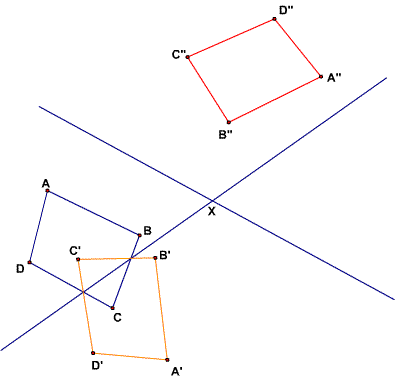
\includegraphics[scale=0.5]{2reflections}
\end{center}
What happens if we change the order of reflections?

\begin{mdsoln}
We will be using directed angles – i.e., all angles are read clockwise and taken modulo $ 180^\circ$.

Suppose we reflect point $ A$ about line $ \ell_1$ to give $ A'$ and then reflect $ A'$ about $ \ell_2$ to give $ A''$. Suppose that $ \ell_1$ and $ \ell_2$ meet at $ X$ and that $ P$ and $ Q$ are points on $ \ell_1$ and $ \ell_2$, respectively.

Observe that $ XA=XA'$ since $ X$ is on $ \ell_1$. Likewise, $ XA''=XA'=XA$. Now,\[ AXA''=\angle A'XA''-\angle A'XA=2\angle A'XQ-2\angle A'XP=2\angle PXQ\]Hence, $ A''$ is the image of $ A$ under a rotation of $ 2\angle PXQ$ (clockwise) about $ X$, which is what we wanted to prove.

If we were to change the order of reflections – i.e., reflect first about $ \ell_2$ and then about $ \ell_1$ - we would get a rotation about twice the other angle between $ \ell_1$ and $ \ell_2$. This would be the same rotation as we originally got, only in the other direction (i.e., counterclockwise instead of clockwise).    
\end{mdsoln}

\subsection{Problem 2}

Prove that the result of rotating a figure about two points, $ Y$, then $ Z$, through angles of $ y$ and $ z$, respectively, is equivalent to a rotation of $ y + z$ about $ X$, where $ X$ is the point such that $ ZYX = y/2$ and $ YZX = z/2$ (with the $ X$ chosen on the appropriate side of $ YZ$).

% https://s3.amazonaws.com/classroom.artofproblemsolving.com/Classes/GeomOlympiad/Images/2rotations.gif
\begin{center}
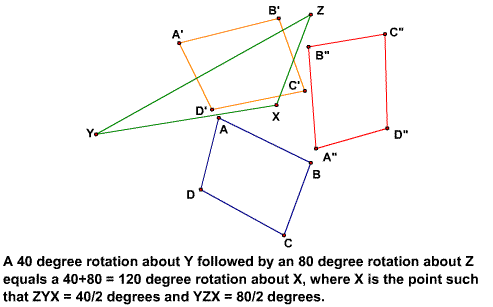
\includegraphics[scale=0.5]{2rotations}
\end{center}

\begin{mdsoln}
Let $ R_1$ denote a rotation of $ y$ about $ Y$ and $ R_2$ denote a rotation of $ z$ about $ Z$. Let $ T$ denote the transformation consisting of $ R_1$ followed by $ R_2$.

Observe that since $ \angle ZYX=y/2$, $ R_1$ takes $ X$ to the reflection $ X'$ of $ X$ over $ YZ$. Then, $ R_2$ takes $ X'$ back to $ X$. Hence, $ X$ is fixed under $ T$.

Let $ A$ be some point distinct from $ X$, with image $ A'$ under $ R_1$ and image $ A''$ under $ T$. We see that since $ T$ is composed of two rotations, it must preserve lengths; namely, $ AX$ must have the same length as its image $ A''X$ under $ T$. Moreover, the line $ AX$ must make an angle of $ y$ with its image $ A'X'$ under $ R_1$ and the line $ A'X'$ must make an angle of $ z$ with its image $ A''X$ under $ R_2$. Hence, $ AX$ must make an angle of $ y+z$ with $ A''X$. We conclude that $ A''$ must be the image of $ A$ under a rotation of $ y+z$ about $ X$, as desired.    
\end{mdsoln}

\subsection{Problem 3}

Squares $ BAXX'$ and $ CAYY'$ are constructed externally on the sides of isosceles triangle $ ABC$ ($ AB = AC$). Let $K$ be a variable point on side $BC$, and let $ E$ and $ F$ be the feet of the perpendiculars from $ K$ to $ CX$ and $ BY$, respectively, and let $ D$ be the midpoint of $ BC$.

a) Prove $ DE = DF$.

b) Find the locus of the midpoint of $ EF$.

% https://s3.amazonaws.com/classroom.artofproblemsolving.com/Classes/GeomOlympiad/Images/turkprob.gif
\begin{center}
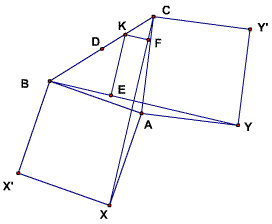
\includegraphics[scale=0.5]{turkprob}
\end{center}
\textit{Has hints.}
\begin{sketch}
    \begin{enumerate}
        \item Show that $ CX = BY$ and that the two segments are perpendicular.
        \item If you haven't tackled Hint 1, use a suitable rotation to prove it quickly.
        \item Let $ P$ be the intersection of $ CX$ and $ BY$. Prove that $ BPC$ is an isosceles right triangle.
        \item Prove that $ BDE$ and $ PDF$ are congruent triangles.
        \item What other segment is the midpoint of $ EF$ also the midpoint of?
    \end{enumerate}
\end{sketch}


\begin{mdsoln}
Note that $ \triangle BAY$ is the image of $ \triangle XAC$ under a rotation of $ 90^\circ$ about $ A$. Hence, if $ P$ is the intersection of $ CX$ and $ BY$, then $ \angle BPC=90^\circ$. By symmetry (about the line $ DA$), $ \triangle BPC$ is an isosceles triangle. Hence, it must be an isosceles right triangle.

Then, $ BD=PD$. Also, since $ KEPF$ is a rectangle, $ BE=BP-EP=CP-KF=CP-CF=PF$. Finally, $ \angle DBE=45^\circ=\angle DPF$. Hence, $ \triangle DBE\cong \triangle DPF$, so $ DE=DF$, as desired.

Note that the midpoint of $ EF$ is also the midpoint of $ KP$. The locus of this midpoint as $ K$ varies along segment $ BC$ is the image of $ BC$ under a dilation of ratio $ 1/2$ centered at $ P$. Hence, the desired locus is the segment connecting the midpoints of $ BP$ and $ CP$.    
\end{mdsoln}

\subsection{Problem 4}

On the sides $ AB$ and $ BC$ of triangle $ ABC$ we construct outward equilateral triangles with vertices $ D$ and $ E$. Show that the midpoints of $ AC$, $ BD$, and $ BE$ are vertices of an equilateral triangle.

% https://s3.amazonaws.com/classroom.artofproblemsolving.com/Classes/GeomOlympiad/Images/threeequil.gif

\begin{center}
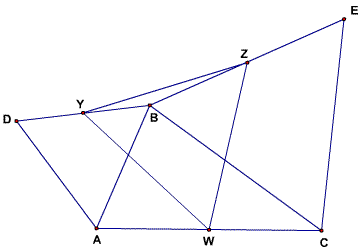
\includegraphics[scale=0.5]{threeequil}
\end{center}
\textit{Has hints.}
\begin{sketch}
    \begin{enumerate}
        \item Look at the points we have and decide which ones we want to be the centers of rotations and dilations. Should any new points be created?
        \item Construct a multi-part transformation, and show that it reduces to a simple rotation.
        \item Show that a 60-degree rotation of one of the points we want to show is on an equilateral triangle about one of the others is the third.
        \item Start with a dilation with ratio 2 and center B.
    \end{enumerate}
\end{sketch}


\begin{mdsoln}
Define the transformation $ T$ as follows: a dilation of ratio 2 about $ B$, then a rotation of $ 60^\circ$ (clockwise for the given diagram) about $ B$, and finally a dilation of ratio $ 1/2$ about $ A$, so that $ T$ takes point $ Z$ to point $ W$.

Observe that $ Y$ is a fixed point under $ T$ (since the component transformations defining $ T$ take $ Y$ to $ D$, then to the reflection $ A'$ of $ A$ over $ DB$, then back to $ Y$). It is evident also that $ T$ preserves lengths (since the component transformations defining $ T$ expand lengths by a factor of 2, then contract them again to their original size). Moreover, the image of a line under $ T$ makes an angle of $ 60^\circ$ (clockwise) with the original line (the component dilations defining $ T$ don’t affect this, since the image of line under a dilation is parallel to the original line).

Hence, $ YZ$ must have the same length as its image $ YW$ under $ T$, and must make angle of $ 60^\circ$ with it. Therefore, $ \triangle YZW$ must be equilateral, as desired.
    
\end{mdsoln}

\subsection{Problem 5}

In the diagram, $ ABC$ is equilateral. Point $ R$ is on $ AB$, $ P$ on $ BC$, and $ Q$ on $ AC$ such that $ ARQ$ and $ BRP$ are equilateral. Point $ N$ is constructed such that $ PQN$ is equilateral. Prove that $ NR$, $ BQ$, and $ AP$ are concurrent.

% https://s3.amazonaws.com/classroom.artofproblemsolving.com/Classes/GeomOlympiad/Images/brotconcur.gif
\begin{center}
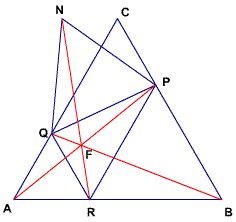
\includegraphics[scale=0.5]{brotconcur}
\end{center}
\textit{Has hints.}
\begin{sketch}
    \begin{enumerate}
        \item Are there any congruent triangles that we can rotate to each other?
        \item Angle chase!
        \item Find a cyclic quadrilateral.
    \end{enumerate}
\end{sketch}

\begin{mdsoln}
Let $ AP$ and $ BQ$ meet at $ F$. We want to show that $ NR$ goes through $ F$.

Observe that $ \triangle QRB$ is the image of $ \triangle ARP$ under a rotation of $ 60^\circ$ about $ R$. Hence, $ \angle BQR=\angle PAR$, so $ FQAR$ is cyclic, implying $ \angle RFQ=180^\circ-\angle QAR=120^\circ$. Likewise, $ FPBR$ is cyclic and $ \angle PFR=120^\circ$.

Hence, $ \angle QFP=120^\circ$, so $ NQFP$ is cyclic, implying that\[ \angle QFN=\angle QPN=60^\circ=180^\circ-\angle RFQ\]so $ F$ lies on $ NR$, as desired.
    
\end{mdsoln}


\chapter{Trigonometry}
\section{Lesson Transcript}
%-- Message Achilleas ( moderator )
% Hi, everyone!

%------------------
%-- Message MeepMurp5 ( user )
% Hi!

%------------------
%-- Message MathJams ( user )
% hi!!

%------------------
%-- Message Ezraft ( user )
% hello!

%------------------
%-- Message chardikala2 ( user )
% Hello!

%------------------
%-- Message bryanguo ( user )
% hi

%------------------
%-- Message pike65_er ( user )
% hi

%------------------
%-- Message RP3.1415 ( user )
% HI!

%------------------
%-- Message Achilleas ( moderator )
% \textbf{Olympiad GeometryWeek 11: Trigonometry}

%------------------
%-- Message Achilleas ( moderator )
% Quick reminder before class starts: I'd like to mention that a class survey has been posted on the course homepage. Please fill the survey out when you get a chance. It helps us to improve our courses and best meet student needs. You can find the survey in the Announcements under the Overview tab.

%------------------
%-- Message Achilleas ( moderator )
Today we'll be talking about applying trigonometry to geometry problems.  Many of you probably do or will use trig as a major crutch for AIME problems, since you can often trig your way through them (with a lot of patience and careful attention to detail).  Unfortunately, slugging through Olympiad problems with trig and analytic geometry usually doesn't work out so well.

%------------------
%-- Message Achilleas ( moderator )
Today we'll discuss some problems in which the tools of trig are either essential or at least very useful.

%------------------
%-- Message Achilleas ( moderator )
Sometimes it's very obvious that trig will help, such as in problems in which some terms in the problem are sines, cosines, or tangents.  Other times it's less obvious.

%------------------
%-- Message Achilleas ( moderator )
As a quick review, here are some important trigonometric formulas. In general, we'll be working with $\triangle ABC$ whose sidelengths are $AB = c, BC = a,$ and $CA = b.$ Additionally, for shorthand, we write $A = \angle BAC, B = \angle ABC,$ and $C = \angle BCA.$

%------------------
%-- Message Achilleas ( moderator )
The \textbf{Law of Cosines} states that $$c^2 = a^2 + b^2 - 2ab\cos{C}.$$ This is crucial for converting between synthetic geometry and algebra.

%------------------
%-- Message Achilleas ( moderator )
The \textbf{Law of Sines} states that $$\frac{a}{\sin{A}} = \frac{b}{\sin{B}} = \frac{c}{\sin{C}} = 2R.$$ That final equality (with $2R$) makes the Law of Sines useful for circumcircles.

%------------------
%-- Message Achilleas ( moderator )
There is also a trigonometric formula for the area of a triangle: $$[ABC] = \frac{1}{2}ab\sin{C}.$$ We'll see this applied in clever ways, especially in conjunction with other area formulas.

%------------------
%-- Message Achilleas ( moderator )
There are plenty of other trigonometric relationships that are useful, and we'll encounter some here and on the message board.  The above are the most frequently useful; many of the others fall under the category 'know that you can prove it quickly, but don't bother memorizing'.

%------------------
%-- Message Achilleas ( moderator )
Now we'll try some problems.  We'll start by discussing some of these trigonometric relationships that you don't need to memorize but should be able to derive should you need them.

%------------------
%-- Message Achilleas ( moderator )
\begin{example}
Express $\displaystyle \tan{\frac{A}{2}}$ in terms of $a,b,$ and $c.$    
\end{example}

%------------------
%-- Message Achilleas ( moderator )
To begin, let's think about the argument: $\displaystyle \tfrac{A}{2}.$ How might we find this angle in $\triangle ABC?$

%------------------
%-- Message TomQiu2023 ( user )
% angle bisector of angle A

%------------------
%-- Message vsar0406 ( user )
% constructing the angle bisector of angle A

%------------------
%-- Message MeepMurp5 ( user )
% the internal angle bisector of $\angle BAC$.

%------------------
%-- Message Catherineyaya ( user )
% draw angle bisector of <BAC

%------------------
%-- Message Bimikel ( user )
% we get the angle bisector of $\angle CAB$

%------------------
%-- Message ca981 ( user )
% using angle bisector on angle A

%------------------
%-- Message Achilleas ( moderator )
Yes! The angle $\frac{A}{2}$ suggests we use the angle bisector of $\angle A.$  But to use the tangent function, we'll need a right angle.  Where will we find one?

%------------------
%-- Message Achilleas ( moderator )
Most of you suggest drawing an altitude. However, what does having an angle bisector already suggests instead?

%------------------
%-- Message Achilleas ( moderator )
% (make sure you give a complete answer; one-word answers are rarely complete)

%------------------
%-- Message Gamingfreddy ( user )
% Draw the incircle?

%------------------
%-- Message coolbluealan ( user )
% drawing the incircle

%------------------
%-- Message Achilleas ( moderator )
% How do we get a right angle?

%------------------
%-- Message MeepMurp5 ( user )
% connect the center of the incircle to the tangent point on $AB$

%------------------
%-- Message vsar0406 ( user )
% draw a radius at a point of tangency between the incircle and a side of the triangle

%------------------
%-- Message chardikala2 ( user )
% draw the line connecting the centre of the incircle to the point of tangency of the incircle and the triangles side

%------------------
%-- Message Catherineyaya ( user )
% line between incenter and tangency point on a side of the triangle is perpendicular to that side (we will use AB or AC)

%------------------
%-- Message Achilleas ( moderator )
As soon as we're talking angle bisectors, we're talking incircle - drawing an inradius gives us our right triangle:

%------------------
%-- Message Achilleas ( moderator )



\begin{center}
\begin{asy}
import cse5;
import olympiad;
//unitsize(4cm);

import markers;
size(150);
pen s = fontsize(8);

/* helper functions */
path scale(real s, pair D, pair E, real p) { return (point(D--E,p)+scale(s)*(-point(D--E,p)+D)--point(D--E,p)+scale(s)*(-point(D--E,p)+E));}
pair r(pair A, pair B, real d){return B = B+rotate(d)*(A-B);}

pair A = dir(210), C = dir(-30), B = dir(110), I = incenter(A,B,C), Y = foot(I,A,C);
draw(incircle(A,B,C),heavygreen);
draw(MP("A",A,dir(210),s)--MP("B",B,dir(110),s)--MP("C",C,dir(-30),s)--cycle);
draw(MP("Y",Y,S,s)--MP("I",I,NE,s)--A^^rightanglemark(I,Y,A,2));

\end{asy}
\end{center}





%------------------
%-- Message Achilleas ( moderator )
Let $Y$ be the tangency point of the incircle with side $AC.$ Now what?

%------------------
%-- Message dxs2016 ( user )
% tan (A/2) = IY/AY

%------------------
%-- Message Catherineyaya ( user )
% tan(A/2)=IY/AY

%------------------
%-- Message mustwin_az ( user )
% tan(A/2)=IY/AY

%------------------
%-- Message RP3.1415 ( user )
% $\tan \frac{A}{2} = \frac{IY}{AY}$

%------------------
%-- Message bryanguo ( user )
% $\tan (\angle IAY) = IY/AY$

%------------------
%-- Message pritiks ( user )
% tan (A/2) = IY/AY

%------------------
%-- Message Achilleas ( moderator )
Because $\displaystyle \angle IAY = \frac{A}{2},$ we have $\displaystyle \tan\frac{A}{2} = \frac{IY}{AY}.$  How can we express $IY$ and $AY?$

%------------------
%-- Message Achilleas ( moderator )
We should be familiar with these calculations involving the incircle by now. How about $IY$ first? What is it equal to?

%------------------
%-- Message dxs2016 ( user )
% radius of incircle

%------------------
%-- Message Ezraft ( user )
% the inradius

%------------------
%-- Message chardikala2 ( user )
% the inradius

%------------------
%-- Message bryanguo ( user )
% $IY$ is the inradius

%------------------
%-- Message Achilleas ( moderator )
We know that $IY$ is the inradius, $r.$

%------------------
%-- Message Achilleas ( moderator )
How about $AY?$

%------------------
%-- Message RP3.1415 ( user )
% $AY=s-a$

%------------------
%-- Message smileapple ( user )
% $AY=s-BC$

%------------------
%-- Message Yufanwang ( user )
% $AY=s-a$

%------------------
%-- Message Achilleas ( moderator )
$AY = s - a,$ where $s$ is the semiperimeter of $\triangle ABC.$ Hence, we have $$\displaystyle\tan\frac{A}{2} = \frac{ r}{s-a}.$$

%------------------
%-- Message Achilleas ( moderator )
Are we done?

%------------------
%-- Message MathJams ( user )
% No, r and s are not in terms of a,b,c

%------------------
%-- Message Catherineyaya ( user )
% we want to express in terms of a,b,c

%------------------
%-- Message RP3.1415 ( user )
% get $r$ and $s$ in terms of $a,b,c$ first

%------------------
%-- Message pritiks ( user )
% no we have to write this expression in terms of a,b, and c

%------------------
%-- Message Bimikel ( user )
% no, we need to express in terms of a, b, and c

%------------------
%-- Message Celwelf ( user )
% No we must convert to a, b, and c

%------------------
%-- Message Lucky0123 ( user )
% No, $r$ and $s$ are not in terms of $a,b,c$

%------------------
%-- Message Achilleas ( moderator )
Not yet. We need our expression to just be in terms of the sidelengths. It's easy to write $s$ like that; by definition, $\displaystyle s = \frac{a+b+c}{2}.$ Now, how can we do it for $r?$

%------------------
%-- Message Achilleas ( moderator )
(be careful; $A$ denotes an angle so far; we can't use for area)

%------------------
%-- Message maxlangy ( user )
% $r=\frac{K}{s} = \frac{\sqrt{(s)(s-a)(s-b)(s-c)}}{s}$, where K denotes area of triangle.

%------------------
%-- Message Gamingfreddy ( user )
% r = sqrt((s-a)(s-b)(s-c)/s)

%------------------
%-- Message J4wbr34k3r ( user )
% $r=\sqrt{\frac{(s-a)(s-b)(s-c)}{s}}$

%------------------
%-- Message Achilleas ( moderator )
Aha! We can write the area of $\triangle ABC$ in two different ways: with Heron's formula (which exclusively involves the sidelengths) and our handy formula $[ABC] = rs,$ which involves the sidenlenghts and the inradius. Perfect! Setting these two formula equal yields:
\begin{align*} rs &= \sqrt{s(s-a)(s-b)(s-c)} \\ \implies r &= \sqrt{\frac{(s-a)(s-b)(s-c)}{s}} \end{align*}

%------------------
%-- Message Achilleas ( moderator )
Now we can finish our original problem. We discovered that $\displaystyle\tan\frac{A}{2} = \frac{r}{s-a}.$ So what's our final answer?

%------------------
%-- Message Achilleas ( moderator )
(we are looking for an equation)

%------------------
%-- Message smileapple ( user )
% $\tan\dfrac{A}{2}=\sqrt{\dfrac{(s-b)(s-c)}{s(s-a)}}$

%------------------
%-- Message Gamingfreddy ( user )
% tan(A/2) = sqrt( (s-b)*(s-c) / (s*(s-a)) )

%------------------
%-- Message vsar0406 ( user )
% tan(A/2) = sqrt((s-b)(s-c)/(s)(s-a))

%------------------
%-- Message TomQiu2023 ( user )
% $\tan(A/2) = \sqrt{\frac{(s-b)(s-c)}{s(s-a)}}$

%------------------
%-- Message Achilleas ( moderator )
Plugging in, we see that $$\displaystyle\tan\frac{A}{2} = \frac{ r}{s-a}= \frac{\sqrt{\frac{(s-a)(s-b)(s-c)}{s}}} {s-a} = \sqrt{\frac{(s-b)(s-c)}{s(s-a)}}.$$

%------------------
%-- Message Achilleas ( moderator )
Great! Now that we're done with that tangent, let's try for cosine!

%------------------
%-- Message Achilleas ( moderator )
\begin{example}
Express $\displaystyle \cos{\frac{A}{2}}$ in terms of $a,b,$ and $c.$    
\end{example}

%------------------
%-- Message Achilleas ( moderator )
How could we begin?

%------------------
%-- Message AOPS81619 ( user )
% Express $\cos x$ in terms of $\tan x$

%------------------
%-- Message Achilleas ( moderator )
Algebraically, how can we relate cosine and tangent?

%------------------
%-- Message Achilleas ( moderator )
(you should not have $\sin x$ in your answers)

%------------------
%-- Message Bimikel ( user )
% $1+\tan^2x=sec^2x$

%------------------
%-- Message AOPS81619 ( user )
% $\tan^2x+1=\frac{1}{\cos^2x}$

%------------------
%-- Message AOPS81619 ( user )
% $\cos x=\sqrt{\frac{1}{1+\tan^2x}}$

%------------------
%-- Message mark888 ( user )
% $\cos(x)=\frac{1}{\sqrt{\tan^2(x)+1}}$

%------------------
%-- Message Achilleas ( moderator )
By Pythagoras, we have $\tan^2\theta + 1 = \sec^2\theta$  so using the fact that secant is the reciprocal of cosine, we can write
$$\cos \theta = \sqrt{\frac{1}{1+\tan^2(\theta)}}.$$

%------------------
%-- Message Achilleas ( moderator )
Now, let's substitute our expression for $\displaystyle \tan\frac{A}{2}$ here:
$$\cos\frac{A}{2} = \sqrt{\frac{1}{1+\frac{(s-b)(s-c)}{s(s-a)}}}= \sqrt{\frac{s(s-a)}{s(s-a)+(s-b)(s-c)}}.$$

%------------------
%-- Message Achilleas ( moderator )
That denominator is a bit of a mess.  Let's see if we can clean that up.  Where might we start?

%------------------
%-- Message maxlangy ( user )
% expand everything?

%------------------
%-- Message Yufanwang ( user )
% Expanding it?

%------------------
%-- Message AOPS81619 ( user )
% expand

%------------------
%-- Message Achilleas ( moderator )
We expand the products, and we have
$$s(s-a) + (s-b)(s-c) = s^2 - as +s^2-bs-cs+bc.$$
That doesn't look much better.  What now?

%------------------
%-- Message MathJams ( user )
% a+b+c = 2s

%------------------
%-- Message Achilleas ( moderator )
Right, we can use the fact that $a+b+c = 2s.$

%------------------
%-- Message Achilleas ( moderator )
How about $-as-bs-cs?$

%------------------
%-- Message coolbluealan ( user )
% it is -2s^2

%------------------
%-- Message Catherineyaya ( user )
% $-as-bs-cs=-(a+b+c)s=-2s^2$

%------------------
%-- Message Wangminqi1 ( user )
% it equals $-2s^2$

%------------------
%-- Message Lucky0123 ( user )
% It is $-2s^2.$

%------------------
%-- Message smileapple ( user )
% $-as-bs-cs=-2s^2$

%------------------
%-- Message Yufanwang ( user )
% $-as-bs-cs=-s(a+b+c)=-2s^2$

%------------------
%-- Message Achilleas ( moderator )
Our expression has $-as-bs-cs,$ which is just $-(a+b+c)(s) = -2s^2.$

%------------------
%-- Message Achilleas ( moderator )
So, what's $s(s-a) + (s-b)(s-c)?$

%------------------
%-- Message coolbluealan ( user )
% $bc$

%------------------
%-- Message MeepMurp5 ( user )
% $bc$

%------------------
%-- Message mustwin_az ( user )
% bc

%------------------
%-- Message MathJams ( user )
% bc

%------------------
%-- Message Ezraft ( user )
% $bc$

%------------------
%-- Message razmath ( user )
% bc

%------------------
%-- Message Trollyjones ( user )
% bc

%------------------
%-- Message AOPS81619 ( user )
% $bc$

%------------------
%-- Message Lucky0123 ( user )
% bc

%------------------
%-- Message dxs2016 ( user )
% bc

%------------------
%-- Message Catherineyaya ( user )
% $s(s-a)+(s-b)(s-c)=bc$

%------------------
%-- Message Bimikel ( user )
% $bc$

%------------------
%-- Message Gamingfreddy ( user )
% s(s-a) + (s-b)(s-c) = bc

%------------------
%-- Message pritiks ( user )
% bc

%------------------
%-- Message Achilleas ( moderator )
That's nice! We have:


\begin{align*}  
    s(s-a) + (s-b)(s-c) &= s^2 - as +s^2-bs-cs+bc\\  
    &=2s^2 -(a+b+c)s + bc\\  
    &=2s^2 -2s^2 + bc\\  
    &= bc.  
    \end{align*}

%------------------
%-- Message Achilleas ( moderator )
In conclusion, we see that
$$\cos\frac{A}{2} = \sqrt{\frac{s(s-a)}{s(s-a)+(s-b)(s-c)}}= \sqrt{\frac{s(s-a)}{bc}}.$$

%------------------
%-- Message Achilleas ( moderator )
And we're done! To finish with all the half-angle trig functions, it's easy to find $\displaystyle \sin \frac{A}{2}$ by multiplying our two previous results.

%------------------
%-- Message Achilleas ( moderator )
\vspace{6pt}
\textbf{Geometric Solution}


Now, let's look for a geometric solution. Seeing that $bc$ sitting in there, and that $s(s-a),$ what tool are we likely to use?

%------------------
%-- Message razmath ( user )
% area?

%------------------
%-- Message AOPS81619 ( user )
% areas?

%------------------
%-- Message MeepMurp5 ( user )
% the area formula?

%------------------
%-- Message smileapple ( user )
% area

%------------------
%-- Message mustwin_az ( user )
% area

%------------------
%-- Message Achilleas ( moderator )
We'll probably break out area.

%------------------
%-- Message Achilleas ( moderator )
We don't have an area expression with cosine.  Where could we start instead?

%------------------
%-- Message Lucky0123 ( user )
% Using the area is $\frac{bc\sin(\angle A)}{2}$

%------------------
%-- Message Achilleas ( moderator )
Right, we know that $[ABC] = \frac{1}{2}bc\sin{A}.$ But we want $\cos \frac{A}{2}.$ Any ideas?

%------------------
%-- Message razmath ( user )
% $\frac{\sin{A}}{2\cos{\frac{A}{2}}} = \sin{\frac{A}{2}}$

%------------------
%-- Message coolbluealan ( user )
% sin(A)=2sin(A/2)cos(A/2)

%------------------
%-- Message Achilleas ( moderator )
Aha, we can apply the double-angle formula for sine. Specifically, $$[ABC] = \frac{1}{2}bc \sin A = \frac{1}{2}bc \cdot 2 \sin \frac{A}{2} \cos \frac{A}{2} = bc \sin \frac{A}{2} \cos \frac{A}{2}.$$

%------------------
%-- Message Achilleas ( moderator )
Okay, we're halfway there! How can we get rid of that pesky $\displaystyle \sin \frac{A}{2} ?$

%------------------
%-- Message mustwin_az ( user )
% its $\cos(A/2) \cdot \tan(A/2)$

%------------------
%-- Message Achilleas ( moderator )
Let's use our previous work. We already discovered that
$$\tan\frac{A}{2} = \sqrt{\frac{(s-b)(s-c)}{s(s-a)}},$$
so we can write
$$\sin\frac{A}{2} = \sqrt{\frac{(s-b)(s-c)}{s(s-a)}}\cdot \cos\frac{A}{2}.$$

%------------------
%-- Message Achilleas ( moderator )
Substituting this into our area formula yields: $$[ABC] = bc \cdot \sqrt{\frac{(s-b)(s-c)}{ s(s-a)}} \cdot \left(\cos\frac{A}{2}\right)^2$$

%------------------
%-- Message Achilleas ( moderator )
Now what?

%------------------
%-- Message AOPS81619 ( user )
% Plug in heron's formula for $[ABC]$

%------------------
%-- Message coolbluealan ( user )
% use heron's formula

%------------------
%-- Message maxlangy ( user )
% use heron's formula for LHS

%------------------
%-- Message razmath ( user )
% $[ABC] = \sqrt{s(s-a)(s-b)(s-c)}$

%------------------
%-- Message Achilleas ( moderator )
Because we need everything in terms of sidelengths, we use Heron to finish. We can substitute $[ABC] = \sqrt{s(s-a)(s-b)(s-c)}$ on the left side. So what's our answer?

%------------------
%-- Message Achilleas ( moderator )
(again, you should give an equation)

%------------------
%-- Message razmath ( user )
% $\cos{\frac{A}{2}} = \sqrt{\frac{s(s-a)}{bc}}$

%------------------
%-- Message dxs2016 ( user )
% cos(A/2)=sqrt(s(s-a)/(bc))

%------------------
%-- Message AOPS81619 ( user )
% $\cos\frac A2=\sqrt{\frac{s(s-a)}{bc}}$

%------------------
%-- Message Catherineyaya ( user )
% $\cos\frac{A}{2}=\sqrt{\frac{s(s-a)}{bc}}$

%------------------
%-- Message Achilleas ( moderator )
A lot of terms cancel, and we find that $$\cos\frac{A}{2} = \sqrt{\frac{s(s-a)}{ bc}}.$$

%------------------
%-- Message Achilleas ( moderator )
Once again, no need to memorize these formulas.  Try to work through the proofs on your own - once you've done so once or twice, it should be clear how you can do so very quickly in the future.

%------------------
%-- Message Achilleas ( moderator )
\begin{remark}
    These two basic examples show how we can relate angles to the sides and use our knowledge of trig functions and identities to find more relationships.  As we've seen above, half-angles are particularly ripe for such approaches.

    %------------------
    %-- Message Achilleas ( moderator )
    Also, area can be a very powerful conduit!
        
\end{remark}

%------------------
%-- Message Achilleas ( moderator )
\begin{example}
Let $ABCD$ be a convex quadrilateral such that $\angle ABC = \angle ADC.$ Define points $M$ and $N$ on $BC$ and $CD$ such that $AM$ is perpendicular to $BC$ and $AN$ is perpendicular to $CD.$  Let point $K$ be the intersection of $BN$ and $DM.$  Prove that line $AK$ is perpendicular to $MN.$    
\end{example}

%------------------
%-- Message Achilleas ( moderator )
First, let's draw ALL of the information into one diagram, so we can understand what it's asking.

%------------------
%-- Message Achilleas ( moderator )



\begin{center}
\begin{asy}
import cse5;
import olympiad;
//unitsize(4cm);

import markers;
size(225);
pen s = fontsize(8);

/* helper functions */
path scale(real s, pair D, pair E, real p) { return (point(D--E,p)+scale(s)*(-point(D--E,p)+D)--point(D--E,p)+scale(s)*(-point(D--E,p)+E));}
pair r(pair A, pair B, real d){return B = B+rotate(d)*(A-B);}

pair D = origin, C = (10,0), B = (12,8), A = extension(D,r(C,D,80),B,r(C,B,-80)) ;
pair M = foot(A,B,C), N = foot(A,C,D), K =extension(B,N,D,M), Q = extension(A,K,N,M);

draw(MP("A",A,NW,s)--MP("B",B,NE,s)--MP("C",C,SE,s)--MP("D",D,SW,s)--cycle);
draw(D--MP("M",M,E,s)--MP("N",N,S,s)--B^^N--A--M^^A--MP("K",K,scale(2)*dir(80),s)--MP("Q",Q,SE,s));
draw(rightanglemark(A,N,D,10)^^rightanglemark(A,M,C,10));

\end{asy}
\end{center}





%------------------
%-- Message Achilleas ( moderator )
Looking at this diagram at a glance, the thing we want to prove involves point $K,$ at the intersection of a lot of lines. What tool does this make us think of?

%------------------
%-- Message dxs2016 ( user )
% ceva

%------------------
%-- Message coolbluealan ( user )
% Ceva's theorem

%------------------
%-- Message Trollface60 ( user )
% ceva's

%------------------
%-- Message MathJams ( user )
% Cevas?

%------------------
%-- Message MTHJJS ( user )
% ceva

%------------------
%-- Message Achilleas ( moderator )
Ceva on $\triangle AMN$ looks like a good choice! If we let $AQ$ be the altitude, then we can re-draw our diagram to focus on these three (hopefully) concurrent cevians.

%------------------
%-- Message Achilleas ( moderator )



\begin{center}
\begin{asy}
import cse5;
import olympiad;
//unitsize(4cm);

unitsize(.8 cm);

pair A, B, D, M, N, Q, K;

A = (0, 0);
D = rotate(315)*(-4,-8);
B = rotate(315)*(6,3);
M = rotate(315)*(6, 0);
N = rotate(315)*(0, -8);
Q = foot(A, M, N);
K = extension(B, N, D, M); 
draw((A--M--N--cycle));
draw(A--D);
draw(A--B);
draw(D--N);
draw(B--M);
draw(N--B, dashed);
draw(M--D, dashed);
draw(A--Q, dashed);
draw(rightanglemark(A,N,D,10)^^rightanglemark(A,M,B,10)^^rightanglemark(A, Q, M, 10));
markscalefactor = 0.1;
draw(anglemark(A,B,M));
draw(anglemark(N,D,A));

label("$A$", A, NE);
label("$B$", B, NE);
label("$D$", D, W);
label("$N$", N, SW);
label("$M$", M, S);
dot("$K$", K, NE);
label("$Q$", Q, S);

\end{asy}
\end{center}





%------------------
%-- Message Achilleas ( moderator )
In effect, we've changed our task from ``Prove that $AK \perp MN$" into ``Prove that $BN, DM,$ and $AQ$ are concurrent."

%------------------
%-- Message MeepMurp5 ( user )
% ceva trig?

%------------------
%-- Message RP3.1415 ( user )
% trig cevas

%------------------
%-- Message Achilleas ( moderator )
Because today is trigonometry day, we won't use typical Ceva. We'll use the sine formulation instead. Thus, we want to prove $$\frac{\sin{\angle ANB}}{\sin{\angle BNM}} \cdot \frac{\sin{\angle NMD}}{\sin{\angle DMA}} \cdot \frac{\sin{\angle MAQ}}{\sin{\angle QAN}} = 1.$$

%------------------
%-- Message Achilleas ( moderator )
Before we dive into the sines, we are going to want to work with very simple angles. So, let's make observations about the angles in the diagram. What do you notice?

%------------------
%-- Message dxs2016 ( user )
% angle DAN = angle BAM

%------------------
%-- Message Catherineyaya ( user )
% $\angle DAN=\angle BAM$

%------------------
%-- Message Achilleas ( moderator )
Right, we observe that $\triangle AND$ and $\triangle AMB$ share two equal angles, so they are similar. In particular, this tells us that $\angle DAN = \angle MAB.$ Let's call this $\alpha.$

%------------------
%-- Message Achilleas ( moderator )
Since we want Ceva to be easy to use, let's define more variables. We can set $\angle MAN = \lambda$ (this is ``lambda.") We can define $\angle ANB = \nu_1$ and $\angle BNM = \nu_2$ (this is pronounced ``nu" for N). Similarly, let $\angle NMD = \mu_1$ and $\angle DMA = \mu_2$ (this is pronounced ``mu" for M). By definitions, $\angle AMN = \mu_1 + \mu_2$ and $ANM = \nu_1 + \nu_2.$ Here's a diagram that shows all these new variables!

%------------------
%-- Message Achilleas ( moderator )



\begin{center}
\begin{asy}
import cse5;
import olympiad;
//unitsize(4cm);

unitsize(.8 cm);

pair A, B, D, M, N, Q, K;
pen s = fontsize(9);

A = (0, 0);
D = rotate(315)*(-4,-8);
B = rotate(315)*(6,3);
M = rotate(315)*(6, 0);
N = rotate(315)*(0, -8);
Q = foot(A, M, N);
K = extension(B, N, D, M); 
draw((A--M--N--cycle));
draw(A--D);
draw(A--B);
draw(D--N);
draw(B--M);
draw(N--B);
draw(M--D);
draw(A--Q, dashed);
draw(arc(A,1/10*length(A-M),degrees(M-A),degrees(N-A)));
draw(rightanglemark(A,M,B,10)^^rightanglemark(A,N,D,10)^^rightanglemark(A,Q,M,10));

//label("$A$", A, scale(3)*dir(-100));
label("$\alpha$",A, scale(5)*dir(-30));
label("$\alpha$",A,scale(4)*dir(-150));
label("$\lambda$",A,scale(4)*dir(-105));
label("$B$", B, NE);
label("$D$", D, W);
label("$\nu_1$", N, scale(10)*dir(30), s);
label("$\nu_2$", N, scale(22)*dir(12), s);
label("$\mu_1$", M, scale(12)*dir(180), s);
label("$\mu_2$", M, scale(6)*dir(150), s);
label("$A$", A, NE);
label("$B$", B, NE);
label("$D$", D, W);
label("$N$", N, SW);
label("$M$", M, S);
dot("$K$", K, NE);
label("$Q$", Q, S);

\end{asy}
\end{center}





%------------------
%-- Message Achilleas ( moderator )
The cevian $AQ$ splits $A$ into two angles: $\angle MAQ$ and $\angle NAQ.$ What are the values of these angles in terms of our new variables?

%------------------
%-- Message Achilleas ( moderator )
How about $\angle MAQ$ first?

%------------------
%-- Message Wangminqi1 ( user )
% $\angle MAQ= 90- \mu_1 - \mu_2$

%------------------
%-- Message AOPS81619 ( user )
% $\angle MAQ=90-\mu_1-\mu_2$

%------------------
%-- Message Achilleas ( moderator )
And how about $\angle NAQ$ first?

%------------------
%-- Message dxs2016 ( user )
% angle NAQ = 90 - v_1 - v_2

%------------------
%-- Message Catherineyaya ( user )
% $\angle NAQ=90^\circ-\nu_1-\nu_2$

%------------------
%-- Message coolbluealan ( user )
% $\angle NAQ =90-\nu_1-\nu_2$

%------------------
%-- Message AOPS81619 ( user )
% $\angle NAQ=90-\nu_1-\nu_2$

%------------------
%-- Message vsar0406 ( user )
% angle NAQ = 90 - v_1 - v_2

%------------------
%-- Message Gamingfreddy ( user )
% Angle NAQ = 90 - v1 - v2

%------------------
%-- Message MeepMurp5 ( user )
% $NAQ = 90^{\circ} - \nu_1 - \nu_2$

%------------------
%-- Message Trollface60 ( user )
% $\angle NAQ = 90 - v1 - v2$

%------------------
%-- Message Achilleas ( moderator )
Right, because $\triangle AMQ$ and $\triangle ANQ$ are right triangles, we have that 


\begin{align*} \angle MAQ &= 90^{\circ} - (\mu_1+\mu_2) \\ \angle NAQ &= 90^{\circ} - (\nu_1+\nu_2). \end{align*}

%------------------
%-- Message Achilleas ( moderator )
Great! Let's rewrite the claim we are trying to prove now: $$\frac{\sin{\nu_1}}{\sin{\nu_2}} \cdot \frac{\sin{\mu_1}}{\sin{\mu_2}} \cdot \frac{\sin{(90^{\circ}-(\mu_1+\mu_2))}}{\sin{(90^{\circ}-(\nu_1+\nu_2))}} = 1.$$

%------------------
%-- Message Achilleas ( moderator )
What's a good tool to help deal with the sines?

%------------------
%-- Message Lucky0123 ( user )
% The law of sines

%------------------
%-- Message mustwin_az ( user )
% Law of Sines

%------------------
%-- Message Achilleas ( moderator )
Right, with the Law of Sines! Let's start with $\sin \nu_1.$ What triangle should we apply the Law of Sines to?

%------------------
%-- Message Achilleas ( moderator )
(Keep in mind, while there are many candidates, we're looking for triangles that work with the variables we've already defined. There's like five of them, after all.)

%------------------
%-- Message pritiks ( user )
% triangle ABN

%------------------
%-- Message MeepMurp5 ( user )
% $\triangle ANB$

%------------------
%-- Message Ezraft ( user )
% $\triangle BAN$

%------------------
%-- Message Catherineyaya ( user )
% triangle NAB

%------------------
%-- Message dxs2016 ( user )
% triangle BNA

%------------------
%-- Message Trollface60 ( user )
% triangle ABN

%------------------
%-- Message Achilleas ( moderator )
It looks like $\triangle BAN$ is a great candidate, and we can rewrite the Law of Sines to see that $$\sin \nu_1 = \frac{AB}{BN}\cdot \sin{(\angle BAN)}.$$ Notice that $\angle BAN = \lambda + \alpha,$ which also happens to be $\angle DAM$. This gives me a good feeling things will cancel eventually.

%------------------
%-- Message Achilleas ( moderator )
What triangle can we use to break down $\sin \nu_2?$

%------------------
%-- Message dxs2016 ( user )
% triangle BNM

%------------------
%-- Message MeepMurp5 ( user )
% $\triangle NBM$

%------------------
%-- Message AOPS81619 ( user )
% $\triangle BMN$

%------------------
%-- Message Catherineyaya ( user )
% triangle BNM

%------------------
%-- Message pritiks ( user )
% triangle NMB

%------------------
%-- Message renyongfu ( user )
% triangle BNM

%------------------
%-- Message Gamingfreddy ( user )
% triangle NBM

%------------------
%-- Message mustwin_az ( user )
% $\triangle BNM$

%------------------
%-- Message bryanguo ( user )
% $\triangle BNM$

%------------------
%-- Message Trollface60 ( user )
% triangle BMN

%------------------
%-- Message Achilleas ( moderator )
We can use $\triangle BMN$ and apply the Law of Sines to see that $\displaystyle \sin \nu_2 = \frac{BM}{BN} \cdot \sin{\angle BMN}.$ What is $\angle BMN$ in terms of our variables?

%------------------
%-- Message Catherineyaya ( user )
% $\angle BMN=90^\circ+\mu_1+\mu_2$

%------------------
%-- Message bryanguo ( user )
% $\angle BMN = 90^\circ +\mu_1+\mu_2$

%------------------
%-- Message Achilleas ( moderator )
We see $\angle BMN = 90^{\circ} + (\mu_1 + \mu_2).$ Now, we can combine our knowledge about $\sin \nu_1$ and $\sin \nu_2$ to find their ratio! $$\frac{\sin \nu_1}{\sin \nu_2} = \frac{\frac{AB}{BN}\cdot \sin{(\lambda+\alpha)}}{\frac{BM}{BN}\cdot \sin{(90^{\circ}+(\mu_1 + \mu_2))}} = \frac{AB}{BM} \cdot \frac{\sin{(\lambda+\alpha)}}{\sin{(90^{\circ}+(\mu_1+\mu_2))}}.$$ Notice how the $BN$'s cancelled because of our well-chosen ratios.

%------------------
%-- Message Achilleas ( moderator )
Great! Now we can attack the next sine ratio on $\mu_1$ and $\mu_2.$ It will be the same process as above, just flipped in the diagram.

%------------------
%-- Message Achilleas ( moderator )
What triangle can we use for $\sin \mu_1?$

%------------------
%-- Message dxs2016 ( user )
% triangle MDN

%------------------
%-- Message Catherineyaya ( user )
% triangle DMN

%------------------
%-- Message pritiks ( user )
% triangle MDN

%------------------
%-- Message mark888 ( user )
% $\triangle DNM$

%------------------
%-- Message vsar0406 ( user )
% triangle DNM

%------------------
%-- Message Bimikel ( user )
% triangle DNM

%------------------
%-- Message ca981 ( user )
% triangle DMN

%------------------
%-- Message AOPS81619 ( user )
% $\triangle DMN$

%------------------
%-- Message mustwin_az ( user )
% $\triangle DMN$

%------------------
%-- Message Gamingfreddy ( user )
% triangle NDM

%------------------
%-- Message Trollyjones ( user )
% triangle DNM

%------------------
%-- Message mathlogic ( user )
% triangle DNM

%------------------
%-- Message razmath ( user )
% $\triangle MDN$

%------------------
%-- Message coolbluealan ( user )
% $\triangle MND$

%------------------
%-- Message dxs2016 ( user )
% triangle MDN.

%------------------
%-- Message TomQiu2023 ( user )
% triangle MND

%------------------
%-- Message pritiks ( user )
% triangle MDN.

%------------------
%-- Message bryanguo ( user )
% triangle DNM

%------------------
%-- Message Ezraft ( user )
% $\triangle DNM$

%------------------
%-- Message christopherfu66 ( user )
% $\triangle MND$

%------------------
%-- Message Achilleas ( moderator )
And what is the resulting equation?

%------------------
%-- Message Achilleas ( moderator )
($\sin \mu_1=?$)

%------------------
%-- Message razmath ( user )
% $\sin{\mu_1} = \sin{(90^{\circ}+\nu_1+\nu_2)}\cdot \frac{DN}{DM}$

%------------------
%-- Message Bimikel ( user )
% $\sin\mu_1=DN/DM*\sin(90^\circ+\nu_1+\nu_2)$

%------------------
%-- Message coolbluealan ( user )
% $\sin \mu_1=\sin(90^\circ+\nu_1+\nu_2)\cdot \frac{DN}{DM}$

%------------------
%-- Message TomQiu2023 ( user )
% $\sin \mu_1 = DN \cdot \sin(90 + \nu_1 + \nu_2) / DM$

%------------------
%-- Message Achilleas ( moderator )
We apply the Law of Sines to $\triangle MND$ to get that $\sin \mu_1 = \frac{DN}{DM} \cdot \sin{(90^{\circ}+(\nu_1 + \nu_2))}.$ And what about for $\sin \mu_2?$

%------------------
%-- Message Achilleas ( moderator )
(note that we use the letters $\mu$ and $\nu$, not u and v)

%------------------
%-- Message Achilleas ( moderator )
% ($\lambda$ is \lambda)

%------------------
%-- Message AOPS81619 ( user )
% $$\sin \mu_2=\frac{DA}{DM}\sin(\lambda+\alpha)$$

%------------------
%-- Message coolbluealan ( user )
% $\sin \mu_2=\sin(\alpha+\lambda)\cdot \frac{DA}{DM}$

%------------------
%-- Message dxs2016 ( user )
% $\sin (\mu_2)=\sin(\lambda + \alpha)\cdot\frac{DA}{DM}$

%------------------
%-- Message Bimikel ( user )
% $\sin \mu_2=(AD/MD)*\sin(\lambda+\alpha)$

%------------------
%-- Message Trollyjones ( user )
% $\sin(\mu_2)=\sin(\alpha+\lambda) \cdot \frac{DA}{DM}$

%------------------
%-- Message MeepMurp5 ( user )
% $\sin \mu_2 = \frac{AD}{MD} \cdot \sin (\lambda + \alpha)$

%------------------
%-- Message razmath ( user )
% $\sin{\mu_2} = \sin{(\lambda+\alpha)}\cdot \frac{AD}{DM}$

%------------------
%-- Message Catherineyaya ( user )
% triangle AMD, $\sin \mu_2=\frac{AD}{DM}\cdot\sin(\alpha+\lambda)$

%------------------
%-- Message Achilleas ( moderator )
We can apply the Law of Sines to $\triangle AMD$ to get that $\sin \mu_2 = \frac{AD}{MD} \cdot \sin{(\lambda + \alpha)}.$ So, we get the ratio:

%------------------
%-- Message Achilleas ( moderator )
$$\frac{\sin \mu_1}{\sin \mu_2} = \frac{\frac{DN}{DM}\cdot \sin{(90^{\circ}+(\nu_1 + \nu_2))}}{\frac{AD}{MD}\cdot \sin{(\lambda + \alpha)}} = \frac{DN}{AD} \cdot \frac{\sin{(90^{\circ}+(\nu_1 + \nu_2))}}{\sin{(\lambda+\alpha)}}.$$

%------------------
%-- Message Achilleas ( moderator )
Great! We've computed our various sine ratios. What now?

%------------------
%-- Message razmath ( user )
% substitute

%------------------
%-- Message mustwin_az ( user )
% Subsitute back in

%------------------
%-- Message MeepMurp5 ( user )
% Plug them in and let them cancel

%------------------
%-- Message dxs2016 ( user )
% plug them back in

%------------------
%-- Message Achilleas ( moderator )
Yeah, we plug into Ceva and hope we get $1!$ We substitute to see:
\begin{align*}
&\frac{\sin{\nu_1}}{\sin{\nu_2}} \cdot \frac{\sin{ \mu_1}}{\sin{\mu_2}} \cdot \frac{\sin{(90^{\circ}-(\mu_1+\mu_2))}}{\sin{(90^{\circ}-(\nu_1+\nu_2))}} \\
&\qquad\qquad= \left( \frac{AB}{BM} \cdot \frac{\sin{(\lambda+\alpha)}}{\sin{(90^{\circ}+(\mu_1+\mu_2))}} \right) \left( \frac{DN}{AD} \cdot \frac{\sin{(90^{\circ}+(\nu_1+\nu_2))}}{\sin{(\lambda+\alpha)}} \right) \left( \frac{\sin{(90^{\circ}-(\mu_1+\mu_2))}}{\sin{(90^{\circ}-(\nu_1+\nu_2))}} \right).
\end{align*}

%------------------
%-- Message Achilleas ( moderator )
Let's see how this cancels! Obviously, $\sin{(\lambda+\alpha)}$ cancels. What else?

%------------------
%-- Message coolbluealan ( user )
% use $\sin(90^\circ+x)=\sin(90^\circ-x)$

%------------------
%-- Message razmath ( user )
% $\sin{(90^{\circ}+X)} = \sin{(90^{\circ}-X)}$

%------------------
%-- Message pritiks ( user )
% sin(90+x) and sin (90-x) cancel eachother

%------------------
%-- Message TomQiu2023 ( user )
% $\sin(90 + (\mu_1 + \mu_2)) = \sin(90 - (\mu_1 + \mu_2))$

%------------------
%-- Message Achilleas ( moderator )
Neat! We notice that $\sin{(90^{\circ} - \theta)} = \sin{(90^{\circ} + \theta)}$ since both are just $\cos \theta.$ So all of the sines cancel out, leaving us with $\frac{AB \cdot DN}{BM \cdot AD}.$ What now?

%------------------
%-- Message AOPS81619 ( user )
% $\triangle AND\sim\triangle AMB$, so $\frac{AB}{BM}=\frac{AD}{DN}$

%------------------
%-- Message Achilleas ( moderator )
Ah, because $\triangle AMB \sim \triangle AND,$ we know that $\frac{AB}{BM} = \frac{AD}{DN},$ which means our desired fraction is just $1!$ We're done.

%------------------
%-- Message razmath ( user )
% is there a non trig way?

%------------------
%-- Message Achilleas ( moderator )
Try to find a non-trig way at your own leisure after class.

%------------------
%-- Message Yufanwang ( user )
% Can we have an idea of a general non-trig path to take?

%------------------
%-- Message Achilleas ( moderator )
The above way does not show a way to think about it.

%------------------
%-- Message Achilleas ( moderator )
Maybe $K$ is the orthocenter of a triangle, but who knows?

%------------------
%-- Message Achilleas ( moderator )
\begin{example}
In triangle $ABC,$ $AC$ is not equal to $BC.$  Assume that the internal bisector of angle $ACB$ bisects also the angle formed by the altitude and the median emanating from vertex $C.$  Show that $ABC$ is a right triangle.    
\end{example}

%------------------
%-- Message Achilleas ( moderator )



\begin{center}
\begin{asy}
import cse5;
import olympiad;
//unitsize(4cm);

import markers;
size(250);
pen s = fontsize(8);

/* helper functions */
path scale(real s, pair D, pair E, real p) { return (point(D--E,p)+scale(s)*(-point(D--E,p)+D)--point(D--E,p)+scale(s)*(-point(D--E,p)+E));}
pair r(pair A, pair B, real d){return B = B+rotate(d)*(A-B);}

pair A = dir(180), B = dir(0), C = dir(120), D = foot(C,A,B), E = extension(C,bisectorpoint(A,C,B),A,B), M = (A+B)/2;
draw(MP("A",A,SW,s)--MP("B",B,SE,s)--MP("C",C,N,s)--cycle);
draw(rightanglemark(C,D,A,2)^^MP("D",D,S,s)--C--MP("M",M,S,s)^^C--MP("E",E,S,s));
markangle(n=2,radius=30,A,C,E,blue);markangle(n=2,radius=32,E,C,B,blue);
markangle(n=1,radius=20,D,C,E,heavyred);markangle(n=1,radius=22,E,C,M,heavyred);

\end{asy}
\end{center}





%------------------
%-- Message Achilleas ( moderator )
There are some slick synthetic methods, but since we see lots of angles, we can pursue a trigonometric approach.

%------------------
%-- Message Achilleas ( moderator )
First I'd do a little angle labeling and some angle chasing.  In particular, with a little work we can get all the angles in the diagram in terms of $A$ and $B.$  At that point, the altitude and bisector (and points $D$ and $E$) don't really even need to be in the diagram, since we're not given any information about them.  The problem then will just be about the median and a handful of angles.

%------------------
%-- Message Achilleas ( moderator )
So let's do this angle chasing.

%------------------
%-- Message Achilleas ( moderator )
Let $\angle DCE = \angle ECM = x$ and $\angle ACD = \angle MCB = y.$  What else do we know?

%------------------
%-- Message Wangminqi1 ( user )
% $\angle A = 90^{\circ}-y$

%------------------
%-- Message AOPS81619 ( user )
% $\angle CBA=90-2x-y$

%------------------
%-- Message Achilleas ( moderator )
We know that $\angle A = 90^{\circ} - y$ from right triangle $ACD,$ and $\angle B = 90^{\circ} - 2x - y$ from right triangle $CBD.$ Hence we can write $y = 90^{\circ} - A$ and $x = \frac{A-B}{2}.$

%------------------
%-- Message Achilleas ( moderator )
(Notice that if we had drawn $AC$ as the larger leg, then $\angle B > \angle A$ and then $x$ would be $\frac{B-A}{2}.$ We won't worry about details like that, but noticing how your diagram affects your results is important!)

%------------------
%-- Message Achilleas ( moderator )
What do we want to prove?

%------------------
%-- Message Trollyjones ( user )
% 2x+2y=90

%------------------
%-- Message SlurpBurp ( user )
% $2x + 2y = 90^\circ$

%------------------
%-- Message mustwin_az ( user )
% 2x+2y=90

%------------------
%-- Message Achilleas ( moderator )
We want to show that $2x+2y = 90,$ which is equivalent to showing that $A + B = 90.$

%------------------
%-- Message Achilleas ( moderator )
Now what?

%------------------
%-- Message Achilleas ( moderator )
Does the law of cosines look helpful?

%------------------
%-- Message Ezraft ( user )
% no

%------------------
%-- Message Achilleas ( moderator )
Not particularly.

%------------------
%-- Message Achilleas ( moderator )
What about the Law of Sines?

%------------------
%-- Message MeepMurp5 ( user )
% I feel like law of sines is better

%------------------
%-- Message Achilleas ( moderator )
On what triangles?

%------------------
%-- Message AOPS81619 ( user )
% $\triangle AMC$ and $\triangle BMC$

%------------------
%-- Message SlurpBurp ( user )
% $\triangle CAM$, $\triangle CBM$

%------------------
%-- Message Achilleas ( moderator )
Why might we focus on triangles $ACM$ and $BCM?$

%------------------
%-- Message razmath ( user )
% since we have $AM = BM$

%------------------
%-- Message AOPS81619 ( user )
% Because we know that $AM=BM$

%------------------
%-- Message SlurpBurp ( user )
% they share side $CM$ and that $AM = MB$

%------------------
%-- Message Achilleas ( moderator )
Triangles $ACM$ and $BCM$ share two side lengths ($CM = CM$ and $AM = BM$), so we can write a relationship regarding the angles of these triangles via the law of sines.  What can we write?

%------------------
%-- Message razmath ( user )
% $\frac{\sin{\angle ACM}}{AM} = \frac{\sin{\angle CAM}}{CM}$ and $\frac{\sin{\angle BCM}}{BM} = \frac{\sin{\angle CBM}}{CM}$

%------------------
%-- Message Achilleas ( moderator )
Yes, we have that $$\frac{AM}{CM} = \frac{\sin \angle ACM}{\sin A}$$ and $$\frac{BM}{CM} = \frac{\sin \angle BCM}{\sin B}.$$

%------------------
%-- Message Achilleas ( moderator )
We know these two are equal, since $AM = BM,$ so we have $$\frac{\sin \angle ACM}{\sin A} = \frac{\sin \angle BCM}{\sin B}.$$

%------------------
%-- Message Achilleas ( moderator )
Now what?

%------------------
%-- Message AOPS81619 ( user )
% Plug in $\angle ACM=y+2x$, $\angle BCM=y$, $\angle A=90-y$, $\angle B=90-2x-y$

%------------------
%-- Message Achilleas ( moderator )
Right, we can write these angles in terms of $A$ and $B.$ Specifically, $\angle ACM = 2x + y = 90^{\circ} - B$ and $\angle BCM = 90^{\circ} - A.$ Plugging this in, we have: $$\frac{\sin{(90^{\circ}-B)}}{\sin A} = \frac{\sin{(90^{\circ}-A)}}{\sin B}.$$

%------------------
%-- Message Achilleas ( moderator )
We finally have our equation relating $A$ and $B!$ What now?

%------------------
%-- Message Lucky0123 ( user )
% We can convert this to $\sin(B)\cos(B) = \sin(A)\cos(A)$

%------------------
%-- Message dxs2016 ( user )
% cosBsinB=sinAcosA?

%------------------
%-- Message Achilleas ( moderator )
We use the fact that $\sin(90^{\circ} - \theta) = \sin \theta.$ Cross-multiplying yields $$\sin A \cos A = \sin B \cos B.$$

%------------------
%-- Message Achilleas ( moderator )
And now?

%------------------
%-- Message AOPS81619 ( user )
% $\sin B\cos B=\sin A\cos A$, so $\sin 2B=\sin 2A$

%------------------
%-- Message dxs2016 ( user )
% sin(2A)=sin(2B)?

%------------------
%-- Message coolbluealan ( user )
% sin(2A)=sin(2B)

%------------------
%-- Message mark888 ( user )
% sin2A=sin2B

%------------------
%-- Message Achilleas ( moderator )
Aha! We multiply both sides by $2$ to apply the sine-double angle formula! This leaves us with $\sin 2A = \sin 2B.$ What can we conclude?

%------------------
%-- Message AOPS81619 ( user )
% Either $A=B$ or $A+B=90$

%------------------
%-- Message mark888 ( user )
% either A=B or 2A+2B=180^circ

%------------------
%-- Message Achilleas ( moderator )
Which case is it?

%------------------
%-- Message Achilleas ( moderator )
And why?

%------------------
%-- Message razmath ( user )
% second case since $BC\neq AC$

%------------------
%-- Message pritiks ( user )
% AC is not equal to BC so A+B=90

%------------------
%-- Message SlurpBurp ( user )
% $A+B = 90^\circ$ since $AC \neq BC$

%------------------
%-- Message coolbluealan ( user )
% A+B=90 becuase AC=/=BC

%------------------
%-- Message mathlogic ( user )
% A+B = 90 beause AC is not equal to BC

%------------------
%-- Message smileapple ( user )
% $A+B=90$, since we are given $\triangle ABC$ is non-iscosceles

%------------------
%-- Message Yufanwang ( user )
% $A+B=90^\circ$ because $AC\neq BC$

%------------------
%-- Message TomQiu2023 ( user )
% $A+B = 90$ since if $A = B$, triangle ABC is isosceles and the problem tells us $AC$ is not equal to $BC$

%------------------
%-- Message Ezraft ( user )
% $A + B = 90^{\circ}$ as $A = B$ implies $AC = BC$ and $AC$ is not equal to $BC$

%------------------
%-- Message MeepMurp5 ( user )
% $A+B = 90^{\circ}$ because $AC \neq BC$, or $\angle CAB \neq \angle CBA$

%------------------
%-- Message mark888 ( user )
% Because AC is not equal to BC, A+B=90 is the answer

%------------------
%-- Message Gamingfreddy ( user )
% A + B = 90, since AC is not equal BC

%------------------
%-- Message ca981 ( user )
% because AC is not equal to BC, so A+B = 90

%------------------
%-- Message Wangminqi1 ( user )
% $A+B=90$ because $ABC$ is not isosceles

%------------------
%-- Message AOPS81619 ( user )
% The problem says that $AC\neq BC$, so we cannot have $A=B$

%------------------
%-- Message Achilleas ( moderator )
Because we are given that $AC \neq BC,$ we know $A \neq B.$ Since the sines of $2A$ and $2B$ are equal, and the angles themselves are not the same, they must be supplementary. This means $2A + 2B = 180^{\circ},$ and thus $A + B = 90^{\circ}.$ Therefore, $\angle C = 90^{\circ},$ so triangle $ABC$ is right.

%------------------
%-- Message Achilleas ( moderator )
\begin{example}
Let $ABCDEF$ be a convex hexagon of perimeter $p$ such that $AB$ is parallel to $DE,$ $BC$ is parallel to $EF$ and $CD$ is parallel to $FA.$ Let $R_A,$ $R_C,$ and $R_E$ denote the circumradii of triangles $FAB,$ $BCD,$ $DEF$ respectively.  Prove that: $$R_A + R_C + R_E \ge \frac{p}{2}$$    
\end{example}

%------------------
%-- Message Achilleas ( moderator )



\begin{center}
\begin{asy}
import cse5;
import olympiad;
//unitsize(4cm);

size(250);
pen s = fontsize(8);

/* helper functions */
path scale(real s, pair D, pair E, real p) { return (point(D--E,p)+scale(s)*(-point(D--E,p)+D)--point(D--E,p)+scale(s)*(-point(D--E,p)+E));}
pair r(pair A, pair B, real d){return B+rotate(d)*(A-B);}

pair A = origin, B = dir(25), C = B+(.8,0), D = C+scale(.9)*rotate(130)*(B-C);
pair E = D+scale(.9)*(A-B), F = extension(A,A+(D-C),E,E+(B-C));
pair W = extension(B,C,A,(0,1)+A), X = extension(B,C,D,(D.x,0)), Y = extension(F,E,D,X), Z = extension(F,E,A,W);
draw(MP("A",A,dir(180),s)--MP("B",B,N,s)--MP("C",C,N,s)--MP("D",D,dir(0),s)--MP("E",E,S,s)--MP("F",F,S,s)--cycle);


\end{asy}
\end{center}





%------------------
%-- Message Achilleas ( moderator )
This problem looks simple.  After working on it a little it may look terrifying.  I'll give you a few minutes to play with it before proceeding.

%------------------
%-- Message Achilleas ( moderator )
What's our initial clue that we might have a trigonometric approach (aside from 'nothing else worked and I pulled out trig in a panic')?

%------------------
%-- Message dxs2016 ( user )
% sine law and its relationship to R

%------------------
%-- Message Ezraft ( user )
% we are given circumradii

%------------------
%-- Message Achilleas ( moderator )
The circumradii suggest that we might use the Law of Sines.  How can we use the Law of Sines here?  Start with $R_A$.

%------------------
%-- Message Achilleas ( moderator )
(we need to use three letters for most angles in this figure)

%------------------
%-- Message dxs2016 ( user )
% FB/sin(FAB) = AF/sin(ABF) = AB/sin(AFB)=2R_A

%------------------
%-- Message Achilleas ( moderator )
Well, the Law of Sines tells us that $$R_A = \frac{BF}{2 \sin A} = \frac{AB}{2 \sin BFA} = \frac{AF}{2 \sin FBA}.$$

%------------------
%-- Message Achilleas ( moderator )
Which of these is most likely to be useful?

%------------------
%-- Message Catherineyaya ( user )
% $R_A=\frac{BF}{2\sin A}$

%------------------
%-- Message MeepMurp5 ( user )
% $R_A = \frac{BF}{2 \sin A}$

%------------------
%-- Message Achilleas ( moderator )
We'll start with the $\sin A$ relationship, because it involves an angle we know something significant about.  What do we know about $\angle A?$

%------------------
%-- Message MathJams ( user )
% <A = <D

%------------------
%-- Message tigerzhang ( user )
% $\angle A=\angle D$

%------------------
%-- Message mustwin_az ( user )
% $\angle A=\angle D$

%------------------
%-- Message coolbluealan ( user )
% $\angle A=\angle D$

%------------------
%-- Message Achilleas ( moderator )
We know that $\angle A = \angle D$ because $BA \parallel DE$ and $AF \parallel CD.$  Now what?

%------------------
%-- Message Achilleas ( moderator )
How can we rewrite $R_A + R_C + R_E $?

%------------------
%-- Message dxs2016 ( user )
% BF/(2sinA)+BD/(2sinC)+DF/(2sinE)

%------------------
%-- Message smileapple ( user )
% $\dfrac{FB}{2\sin A}+\dfrac{BD}{2\sin C}+\dfrac{DF}{2\sin E}$

%------------------
%-- Message mark888 ( user )
% $\frac{BF}{2\sin(A)}+\frac{BD}{2\sin(C)}+\frac{DF}{2\sin(E)}$

%------------------
%-- Message smileapple ( user )
% $R_A+R_C+R_E=\dfrac{FB}{2\sin A}+\dfrac{BD}{2\sin C}+\dfrac{DF}{2\sin E}$

%------------------
%-- Message MathJams ( user )
% BF/(2sin A) +BD/(2sin C) +DF/(2sin E)

%------------------
%-- Message Achilleas ( moderator )
Right, we can do the same for the others, and we thus have: $$R_A + R_C + R_E = \frac{BF}{2\sin A} + \frac{BD}{2 \sin C} + \frac{DF}{2 \sin E}.$$

%------------------
%-- Message Achilleas ( moderator )
Hmm…  Now what?  We need to knock out those sines, and we need to convert the $BF, BD, DF$ to the sides of the hexagon somehow.

%------------------
%-- Message Achilleas ( moderator )
I'm going to let you all think about this for a few minutes before continuing.

%------------------
%-- Message Achilleas ( moderator )
(no, the law of cosines does not help)

%------------------
%-- Message Achilleas ( moderator )
We have sines, we want to relate them to side lengths.  We've already used the law of sines.  What other way can we relate sines to side lengths?

%------------------
%-- Message Achilleas ( moderator )
(area is a popular idea, but nope)

%------------------
%-- Message Achilleas ( moderator )
(Recall how you first learned or defined what the sine of an angle is)

%------------------
%-- Message Achilleas ( moderator )
What shapes did you use?

%------------------
%-- Message MathJams ( user )
% making some right triangles?

%------------------
%-- Message pritiks ( user )
% creating some right triangles

%------------------
%-- Message mustwin_az ( user )
% Right triangles

%------------------
%-- Message TomQiu2023 ( user )
% right triangles

%------------------
%-- Message MeepMurp5 ( user )
% right triangles

%------------------
%-- Message Ezraft ( user )
% right triangles

%------------------
%-- Message AOPS81619 ( user )
% right triangles

%------------------
%-- Message Achilleas ( moderator )
Right triangles give us a way to relate sines to side lengths.  Do we have any right triangles?

%------------------
%-- Message Ezraft ( user )
% no

%------------------
%-- Message bryanguo ( user )
% no

%------------------
%-- Message Achilleas ( moderator )
Nope.  No right triangles.  Can we construct any?  We want right triangles that involve the sides of the hexagon and the angles of the hexagon.  What's hard about making right triangles that involve the angles of the hexagon?

%------------------
%-- Message Trollyjones ( user )
% we don't know the angles measurements

%------------------
%-- Message SlurpBurp ( user )
% they can be obtuse?

%------------------
%-- Message Achilleas ( moderator )
The angles of the hexagon might all be obtuse - tough to make right triangles with obtuse angles.  Are we stuck?  Should we give up on right triangles?

%------------------
%-- Message dxs2016 ( user )
% exterior ones?

%------------------
%-- Message Bimikel ( user )
% maybe extend some lines

%------------------
%-- Message Achilleas ( moderator )
We don't have to give up on right triangles quite yet.  Because $\sin(x) = \sin(180-x),$ we'd be happy to find right triangles with angles which are supplementary to the angles of the hexagon.  This gives us a huge clue where to look for them - where?

%------------------
%-- Message bryanguo ( user )
% extend side lenghts?

%------------------
%-- Message Achilleas ( moderator )
We look outside the hexagon.  We can extend two opposite sides and ultimately build a rectangle around our hexagon:

%------------------
%-- Message Achilleas ( moderator )



\begin{center}
\begin{asy}
import cse5;
import olympiad;
//unitsize(4cm);

size(250);
pen s = fontsize(8);

/* helper functions */
path scale(real s, pair D, pair E, real p) { return (point(D--E,p)+scale(s)*(-point(D--E,p)+D)--point(D--E,p)+scale(s)*(-point(D--E,p)+E));}
pair r(pair A, pair B, real d){return B+rotate(d)*(A-B);}

pair A = origin, B = dir(25), C = B+(.8,0), D = C+scale(.9)*rotate(130)*(B-C);
pair E = D+scale(.9)*(A-B), F = extension(A,A+(D-C),E,E+(B-C));
pair W = extension(B,C,A,(0,1)+A), X = extension(B,C,D,(D.x,0)), Y = extension(F,E,D,X), Z = extension(F,E,A,W);
draw(MP("A",A,dir(180),s)--MP("B",B,N,s)--MP("C",C,N,s)--MP("D",D,dir(0),s)--MP("E",E,S,s)--MP("F",F,S,s)--cycle);

draw(MP("W",W,NW,s)--MP("X",X,NE,s)--MP("Y",Y,SE,s)--MP("Z",Z,SW,s)--cycle);
draw(rightanglemark(B,W,A,2)^^rightanglemark(A,Z,F,2)^^rightanglemark(E,Y,D,2)^^rightanglemark(D,X,C,2),heavyred);

\end{asy}
\end{center}





%------------------
%-- Message Achilleas ( moderator )
Now we have right triangles!

%------------------
%-- Message Achilleas ( moderator )
Throughout the problem, I will continue to use just $A, B,$ etc to refer to the angles of the hexagon.  Use three letters if you want to talk about the angles outside the hexagon in the right triangle.

%------------------
%-- Message Achilleas ( moderator )
The right triangles come in two pairs of similar triangles: $\triangle ABW \sim \triangle DEY$ and $\triangle DCX \sim \triangle AFZ.$   How does this help us with our problem?

%------------------
%-- Message Achilleas ( moderator )
Note that we are interested in the sines of the acute angles in the right triangles.

%------------------
%-- Message Achilleas ( moderator )
Specifically, we see that: $$R_A + R_C + R_E = \frac{BF}{2\sin A} + \frac{BD}{2 \sin C} + \frac{DF}{2 \sin E}.$$

%------------------
%-- Message Achilleas ( moderator )
So?

%------------------
%-- Message MathJams ( user )
% We have more ratios?

%------------------
%-- Message Achilleas ( moderator )
We wish to relate these to lengths, so we use our right triangles: $$\frac{AW}{AB} = \sin \angle ABW = \sin B = \sin E = \sin \angle DEY = \frac{DY}{DE}.$$

%------------------
%-- Message Achilleas ( moderator )
Similarly, we have $$\frac{AZ}{AF} = \sin \angle AFZ = \sin F = \sin C = \sin \angle DCX = \frac{DX}{CD}.$$

%------------------
%-- Message Achilleas ( moderator )
Have you followed everything in this problem so far?

%------------------
%-- Message pritiks ( user )
% yes.

%------------------
%-- Message TomQiu2023 ( user )
% yes

%------------------
%-- Message bryanguo ( user )
% yes

%------------------
%-- Message Ezraft ( user )
% yes

%------------------
%-- Message Achilleas ( moderator )
Great! In our complicated expression for $R_A + R_C + R_E,$ we have expressions for our sines. Now, onto the sidelengths.

%------------------
%-- Message Achilleas ( moderator )
We also know we need to have an inequality in the end, and we need to get rid of those 2's.

%------------------
%-- Message Achilleas ( moderator )
How can we deal with $BF, BD, DF?$

%------------------
%-- Message Achilleas ( moderator )
How about $BF$ first?

%------------------
%-- Message Achilleas ( moderator )
Well, the triangle inequality gives us $BF < AB + AF$, so that
$$\frac{BF}{2 \sin A} < \frac{AB + AF}{2 \sin A}.$$

%------------------
%-- Message Achilleas ( moderator )
Is this going to help?  Why or why not?

%------------------
%-- Message smileapple ( user )
% no because we want $BF$ to be in the upper bound

%------------------
%-- Message coolbluealan ( user )
% no, the problem has a greater than or equal to

%------------------
%-- Message Achilleas ( moderator )
This is probably not going to help because the inequality is going the wrong way.

%------------------
%-- Message Achilleas ( moderator )
So, we shelve the triangle inequality for now and look for others.  Don't forget it entirely, just don't bother wasting an hour barking up that tree right now.  You should in general always be doing this before barreling down a path you find - ask yourself how feasible it is to be helpful.  Make sure there aren't any pretty clear negative signs like the one we just found before wasting 30 minutes digging yourself deeper.  Consider your alternatives first.

%------------------
%-- Message Achilleas ( moderator )
This is especially important on harder problems - red herrings and blind alleys can cost you tons of time.  I imagine most students who saw this problem when it was first given in a contest got stuck right here - heading down the triangle inequality path, never to be heard from again.

%------------------
%-- Message Achilleas ( moderator )
We'd like $BF \geq something,$ so we want $BF$ on the big side.  What is it larger than or equal to?

%------------------
%-- Message MTHJJS ( user )
% BF >= WZ

%------------------
%-- Message smileapple ( user )
% $BF\ge WZ$

%------------------
%-- Message Achilleas ( moderator )
We know that $BF \geq WZ = AW + AZ.$  Why does this look promising?

%------------------
%-- Message MathJams ( user )
% Since they are parts of our sin ratios

%------------------
%-- Message J4wbr34k3r ( user )
% Expressible in terms of side lengths and angle measures.

%------------------
%-- Message Achilleas ( moderator )
One reason is that this inequality is sharp (in other words, for some configurations of the diagram, it becomes an equality) and the corresponding inequalities for the other two lengths can simultaneously be equalities.  (Think of a regular hexagon.)  It's nice to have a sharp inequality because it gives us a reason to think the right hand side might be provably greater than or equal to what we want (in this case, $\frac{p}{2}$).

%------------------
%-- Message Achilleas ( moderator )
It also looks promising because we can write $AW$ and $AZ$ in terms of sines: $AW = AB\sin B$; $AZ = AF\sin F = AF\sin C$ .  Now, substitution is much happier:

%------------------
%-- Message Achilleas ( moderator )
$$\frac{BF}{2 \sin A}\ge \frac{AW + AZ}{2 \sin A} = \frac{AB}{2}\cdot \frac{\sin B}{\sin A} + \frac{AF}{2}\cdot \frac{\sin C}{\sin A}.$$

%------------------
%-- Message Achilleas ( moderator )
This expression looks considerably nicer.  What happens if we try it on the other two terms in our expression for $R_A + R_C + R_E?$

%------------------
%-- Message Achilleas ( moderator )
What would we need to do first, though?

%------------------
%-- Message Achilleas ( moderator )
(recall how we found the above inequality)

%------------------
%-- Message AOPS81619 ( user )
% Draw different rectangles

%------------------
%-- Message Achilleas ( moderator )
We can construct rectangles around the hexagon in other orientations to show that: $$ \frac{BD}{2 \sin C} \ge\frac{CD}{2}\cdot \frac{\sin A}{\sin C}  + \frac{BC}{2} \cdot \frac{\sin B}{\sin C} $$ and  $$\frac{DF}{2 \sin E} \ge \frac{DE}{2}\cdot \frac{\sin A}{\sin B} + \frac{EF}{2}\cdot \frac{\sin C}{\sin B}. $$

%------------------
%-- Message Achilleas ( moderator )



\begin{center}
\begin{asy}
import cse5;
import olympiad;
//unitsize(4cm);

size(500);
pen s = fontsize(8);

/* helper functions */
path scale(real s, pair D, pair E, real p) { return (point(D--E,p)+scale(s)*(-point(D--E,p)+D)--point(D--E,p)+scale(s)*(-point(D--E,p)+E));}
pair r(pair A, pair B, real d){return B+rotate(d)*(A-B);}

pair A = origin, B = dir(25), C = B+(.8,0), D = C+scale(.9)*rotate(130)*(B-C);
pair E = D+scale(.9)*(A-B), F = extension(A,A+(D-C),E,E+(B-C));
//pair W = extension(B,C,A,(0,1)+A), X = extension(B,C,D,(D.x,0)), Y = extension(F,E,D,X), Z = extension(F,E,A,W);
pair O = extension(A,B,D,D+rotate(-90)*(E-D)), N = foot(C,B,O), P = foot(C,O,D);
pair L = extension(E,D,A,A+rotate(-90)*(B-A)), M = foot(F,E,D), K = foot(F,A,L);

draw(MP("A",A,dir(180),s)--MP("B",B,dir(90),s)--MP("C",C,dir(-130),s)--MP("D",D,dir(0),s)--MP("E",E,S,s)--MP("F",F,dir(70),s)--cycle);

draw(B--MP("O",O,dir(90),s)--D^^MP("N",N,dir(130),s)--C--MP("P",P,dir(0),s)^^A--MP("L",L,dir(-90),s)--E^^MP("K",K,SW,s)--F--MP("M",M,SE,s));

//draw(MP("W",W,NW,s)--MP("X",X,NE,s)--MP("Y",Y,SE,s)--MP("Z",Z,SW,s)--cycle);
draw(rightanglemark(K,L,M,1.5)^^rightanglemark(L,K,F,1.5)^^rightanglemark(K,F,M,1.5)^^rightanglemark(B,N,C,1.5)^^rightanglemark(N,O,P,1.5)^^rightanglemark(O,P,C,1.5)^^rightanglemark(O,D,L,1.5),heavyred);

draw(minipage("Here the rectangle $LAOD$ has $AB$ and $DE$ along its sides. We project $C$ and $F$ onto the rectangle sides to see the right triangles.",8cm),D,shift(0,15)*scale(15)*dir(0),s);

draw(minipage("\centering$BD\geq PD+ CN$",8cm),D,shift(0,10)*scale(15)*dir(0),s);
draw(minipage("\centering$\frac{PD}{CD} = \cos PDC = \sin D \quad$ (from ${PCD})$",8cm),D,shift(13,3)*scale(15)*dir(0),s);
draw(minipage("\centering$\frac{CN}{BC} = \sin CBN = \sin B \quad$ (from ${BCD})$",8cm),D,shift(13,-4)*scale(15)*dir(0),s);
draw(minipage("\centering$\frac{BC}{2 \sin C} \geq \frac{PD + CN}{2 \sin C}$",8cm),D,shift(0,-11)*scale(15)*dir(0),s);
draw(minipage("\centering$= \frac{CD \sin D}{2 \sin C} + \frac{BC\sin B}{2\sin C}$",8cm),D,shift(14,-20)*scale(15)*dir(0),s);
draw(minipage("\centering$= \frac{CD \sin A}{2 \sin C} + \frac{BC\sin C}{2\sin C}$",8cm),D,shift(14,-29)*scale(15)*dir(0),s);


\end{asy}
\end{center}





%------------------
%-- Message Achilleas ( moderator )



\begin{center}
\begin{asy}
import cse5;
import olympiad;
//unitsize(4cm);

size(500);
pen s = fontsize(8);

/* helper functions */
path scale(real s, pair D, pair E, real p) { return (point(D--E,p)+scale(s)*(-point(D--E,p)+D)--point(D--E,p)+scale(s)*(-point(D--E,p)+E));}
pair r(pair A, pair B, real d){return B+rotate(d)*(A-B);}

pair A = origin, B = dir(25), C = B+(.8,0), D = C+scale(.9)*rotate(130)*(B-C);
pair E = D+scale(.9)*(A-B), F = extension(A,A+(D-C),E,E+(B-C));
//pair W = extension(B,C,A,(0,1)+A), X = extension(B,C,D,(D.x,0)), Y = extension(F,E,D,X), Z = extension(F,E,A,W);
pair R = extension(C,D,A,A+rotate(90)*(F-A)), Q = foot(B,R,A), S = foot(B,R,D);
pair U = extension(A,F,D,D+rotate(-90)*(C-D)), T = foot(E,U,D), V = foot(E,A,F);

draw(MP("A",A,dir(180),s)--MP("B",B,dir(-90),s)--MP("C",C,dir(-130),s)--MP("D",D,dir(0),s)--MP("E",E,dir(90),s)--MP("F",F,dir(70),s)--cycle);
draw(A--MP("R",R,dir(90),s)--D^^MP("Q",Q,dir(135),s)--B--MP("S",S,dir(45),s)^^F--MP("U",U,dir(-90),s)--D^^MP("V",V,dir(-150),s)--E--MP("T",T,dir(-45),s));

draw(rightanglemark(Q,A,V,1.5)^^rightanglemark(F,V,E,1.5)^^rightanglemark(F,U,T,1.5)^^rightanglemark(E,T,D,1.5)^^rightanglemark(T,D,C,1.5)^^rightanglemark(C,S,B,1.5)^^rightanglemark(C,R,Q,1.5)^^rightanglemark(R,Q,B,1.5),heavyred);

draw(minipage("Here the rectangle $RDUA$ has $AF$ and $CD$ along its sides. We project $B$ and $E$ onto the rectangle sides to see the right triangles.",8cm),D,shift(0,15)*scale(15)*dir(0),s);

draw(minipage("\centering$DF\geq DT+ EV$",8cm),D,shift(0,10)*scale(15)*dir(0),s);
draw(minipage("\centering$\frac{DT}{DE} = \cos EDT = \sin D \quad$ (from ${DET})$",8cm),D,shift(13,3)*scale(15)*dir(0),s);
draw(minipage("\centering$\frac{EV}{EF} = \sin EFV = \sin F \quad$ (from ${EFV})$",8cm),D,shift(13,-4)*scale(15)*dir(0),s);
draw(minipage("\centering$\frac{DF}{2 \sin E} \geq \frac{DT + EV}{2 \sin E}$",8cm),D,shift(0,-11)*scale(15)*dir(0),s);
draw(minipage("\centering$= \frac{DE \sin D}{2 \sin E} + \frac{EF\sin F}{2\sin E}$",8cm),D,shift(14,-20)*scale(15)*dir(0),s);
draw(minipage("\centering$= \frac{DE \sin A}{2 \sin B} + \frac{EF\sin C}{2\sin B}$",8cm),D,shift(14,-29)*scale(15)*dir(0),s);


\end{asy}
\end{center}





%------------------
%-- Message Achilleas ( moderator )
What happens when we add these?

%------------------
%-- Message Achilleas ( moderator )
When we add these we see that we are painfully close to the solution, as we then have

%------------------
%-- Message Achilleas ( moderator )
\begin{align*}  
    R_A + R_C + R_E &\ge \frac{AB}{2}\cdot\frac{\sin B}{\sin A} + \frac{AF}{2}\cdot \frac{\sin C}{\sin A} + \frac{BC}{2}\cdot \frac{\sin B}{\sin C} \\  
    &\quad+ \frac{CD}{2}\cdot\frac{\sin A}{\sin C} + \frac{DE}{2}\cdot \frac{\sin A}{\sin B} + \frac{EF}{2}\cdot\frac{\sin C}{\sin B}.\end{align*}

%------------------
%-- Message Achilleas ( moderator )
What do you notice?

%------------------
%-- Message Lucky0123 ( user )
% There is a factor of $1/2$ on the RHS, as desired

%------------------
%-- Message pritiks ( user )
% when the sine terms are all multiplied together they equal 1 and the other terms equal p/2

%------------------
%-- Message MeepMurp5 ( user )
% reciprocals of each other for the ratio of the sines

%------------------
%-- Message Achilleas ( moderator )
We see terms like $\frac{\sin B}{\sin A}$ and their reciprocal. If we could just get these added together, we'd be able to get rid of them since their sum must be greater than or equal to $2$ (since $x + x^{-1} \geq 2$ for all positive $x$).  Unfortunately, we can't group them.

%------------------
%-- Message Achilleas ( moderator )
Some of you suggest AM-GM but it is not immediately clear how this applies, since we would get the product of side-lengths of the hexagon.

%------------------
%-- Message smileapple ( user )
% $\dfrac{\sin B}{\sin A}+\dfrac{\sin A}{\sin B}\ge 2$ by AM-GM

%------------------
%-- Message Achilleas ( moderator )
True, but what happens to the side-lengths in front of these fractions?

%------------------
%-- Message Achilleas ( moderator )
If only we had a ($AB/2)(\sin A/\sin B)$ term to go with the $(AB/2)(\sin B/\sin A)$ term.  Add em up, say they're $\ge AB$.  Same goes for each of the other terms.  This gets us thinking what?

%------------------
%-- Message Achilleas ( moderator )
\vspace{6pt}
\textbf{Hint:} The side-lengths appear only once on the right side above.

%------------------
%-- Message smileapple ( user )
% double it?

%------------------
%-- Message Achilleas ( moderator )
% Double what?

%------------------
%-- Message Achilleas ( moderator )
We need to double the number of terms we have somewhere in our string of reasoning.  Now we wander deep into wishful thinking land (where many wonderful solutions are hiding) and go looking for our extra terms.  We go step by step through our solution so far:

%------------------
%-- Message Achilleas ( moderator )
First, Law of Sines gave us:

%------------------
%-- Message Achilleas ( moderator )
$$R_A + R_C + R_E = \frac{BF}{2\sin A} + \frac{BD}{2 \sin C} + \frac{DF}{2 \sin E}.$$

%------------------
%-- Message Achilleas ( moderator )
Anything there?

%------------------
%-- Message Ezraft ( user )
% no

%------------------
%-- Message Achilleas ( moderator )
Nothing really looks good here.  Take a look at the next step:

%------------------
%-- Message Achilleas ( moderator )
$$BF \ge ZW = AW + AZ.$$

%------------------
%-- Message Achilleas ( moderator )
Could we have doubled the number of terms here by doing something different?

%------------------
%-- Message JacobGallager1 ( user )
% We can also say that $BF \geq XD + DY$

%------------------
%-- Message Trollyjones ( user )
% how about BF >=XY=XD+DY

%------------------
%-- Message coolbluealan ( user )
% XD+DY=AW+AZ

%------------------
%-- Message smileapple ( user )
% $2BF\ge WA+AZ+XD+DY?$

%------------------
%-- Message Achilleas ( moderator )
Aha! Because we inscribed the hexagon into a rectangle, the opposite sides are equal. Specifically, this means that $ZW = \frac{ZW + XY}{2}.$

%------------------
%-- Message JacobGallager1 ( user )
% So we can write $BF \geq \frac{AW + AZ + XD + DY}{2}$

%------------------
%-- Message Achilleas ( moderator )
Hence, $$BF \geq ZW = \frac{ZW + XY}{2} = \frac{AW+AZ+XD+XY}{2}.$$

%------------------
%-- Message Achilleas ( moderator )
Because of all the rectangles, we can rewrite all four terms of the above using sines. We observe: $$\frac{BF}{2 \sin A}\ge \frac{AW+AZ+XD+XY}{4 \sin A} =\frac{AB}{4}\cdot \frac{\sin B}{\sin A} + \frac{AF}{4}\cdot\frac{\sin C}{\sin A} + \frac{CD}{4}\cdot \frac{\sin C}{\sin A} + \frac{DE}{4}\cdot \frac{\sin B}{\sin A}.$$

%------------------
%-- Message Achilleas ( moderator )
There are our extra terms!  Let's do the same for the other two: 


$$\frac{BD}{2 \sin C} \geq \frac{CD}{4} \cdot \frac{\sin A}{\sin C} + \frac{BC}{4} \cdot \frac{\sin B}{\sin C} + \frac{AF}{4} \cdot \frac{\sin A}{\sin C} + \frac{EF}{4} \cdot \frac{\sin B}{\sin C}$$


    and


$$\frac{DF}{2 \sin E} \geq \frac{DE}{4} \cdot \frac{\sin A}{\sin B} + \frac{EF}{4} \cdot \frac{\sin C}{\sin B} + \frac{AB}{4} \cdot \frac{\sin A}{\sin B} + \frac{BC}{4} \cdot \frac{\sin C}{\sin B}.$$

%------------------
%-- Message Achilleas ( moderator )
How many times does $AB$, for example, appear in the above sums (in total)?

%------------------
%-- Message Lucky0123 ( user )
% Twice

%------------------
%-- Message mustwin_az ( user )
% twice

%------------------
%-- Message Trollyjones ( user )
% two times

%------------------
%-- Message Gamingfreddy ( user )
% Twice

%------------------
%-- Message JacobGallager1 ( user )
% Twice

%------------------
%-- Message dxs2016 ( user )
% 2

%------------------
%-- Message coolbluealan ( user )
% 2

%------------------
%-- Message ca981 ( user )
% twice

%------------------
%-- Message Achilleas ( moderator )
It appears twice.

%------------------
%-- Message Achilleas ( moderator )
Great! What now?

%------------------
%-- Message dxs2016 ( user )
% add them up?

%------------------
%-- Message Achilleas ( moderator )
Addition brings us home.  If we add our expressions that are less than or equal to $R_A, R_C,$ and $R_E,$ we see that we can pair up all the terms to create our $x + x^{-1}$ scenarios.

%------------------
%-- Message Achilleas ( moderator )
For example, what is the sum of the terms that involve $DE$?

%------------------
%-- Message JacobGallager1 ( user )
% $\frac{DE}{4} \cdot \frac{\sin A}{\sin B} + \frac{DE}{4} \cdot \frac{\sin B}{\sin A} $

%------------------
%-- Message dxs2016 ( user )
% (DE/4) * (sinB/sinA + sinA/sinB)

%------------------
%-- Message Trollyjones ( user )
% $\frac{DE}{4} \cdot \frac{\sin B}{\sin A}+\frac{DE}{4} \cdot \frac{\sin A}{\sin B}$

%------------------
%-- Message smileapple ( user )
% $\dfrac{DE}{4}\left(\dfrac{\sin B}{\sin A}+\dfrac{\sin A}{\sin B}\right)$

%------------------
%-- Message Achilleas ( moderator )
It is  $$\frac{DE}{4}\cdot\frac{\sin A}{\sin B} + \frac{DE}{4}\cdot\frac{\sin B}{\sin A} $$.

%------------------
%-- Message Achilleas ( moderator )
Now, what?

%------------------
%-- Message smileapple ( user )
% $\dfrac{DE}{4}\left(\dfrac{\sin B}{\sin A}+\dfrac{\sin A}{\sin B}\right)\ge \dfrac{DE}{2}$

%------------------
%-- Message JacobGallager1 ( user )
% $\frac{DE}{4} \cdot \frac{\sin A}{\sin B} + \frac{DE}{4} \cdot \frac{\sin B}{\sin A} \geq \frac{DE}{4} \cdot 2 = \frac{DE}{2}$

%------------------
%-- Message Achilleas ( moderator )
We see that $$\frac{DE}{4}\cdot\frac{\sin A}{\sin B} + \frac{DE}{4}\cdot\frac{\sin B}{\sin A} = \frac{DE}{4}\left(\frac{\sin A}{\sin B} + \frac{\sin B}{\sin A}\right) \ge \frac{DE}{4}\cdot 2 = \frac{DE}{2}.$$

%------------------
%-- Message Lucky0123 ( user )
% We know that this sum $\ge \frac{DE}{2},$ so adding up all the other terms of this type will get $p/2$

%------------------
%-- Message Trollyjones ( user )
% similar for the oterh terms

%------------------
%-- Message Achilleas ( moderator )
Summing across all of our expressions yields $$R_A + R_C + R_E \ge \frac{AB}{2} + \frac{BC}{2} + \frac{CD}{2} + \frac{DE}{2} + \frac{EF}{2} + \frac{FA}{2} = \frac{AB+BC+CD+DE+EF+FA}{2},$$ as desired. Problem complete!

%------------------
%-- Message RP3.1415 ( user )
% nice!

%------------------
%-- Message Ezraft ( user )
% that was a really long problem

%------------------
%-- Message bryanguo ( user )
% hard problem

%------------------
%-- Message Achilleas ( moderator )
This problem has been described by some as the most difficult IMO problem ever (judging by the scores of the participants, I think it was the hardest through the late 90s or so).

%------------------
%-- Message smileapple ( user )
% it was in the IMO!????!??

%------------------
%-- Message Achilleas ( moderator )
% Yup!

%------------------
%-- Message Achilleas ( moderator )
If you got a little lost as we went through the problem, take the time to walk through the steps again later.  Try to understand both why each step is true, and why we thought to make each step.

%------------------
%-- Message RP3.1415 ( user )
% oh wow what problem was it?!

%------------------
%-- Message Achilleas ( moderator )
\#5 in IMO 1996.

%------------------
%-- Message Achilleas ( moderator )
Ciprian Manolescu's beautiful solution during the contest used and proved a generalization of the Erdos-Mordell inequality.

%------------------
%-- Message Achilleas ( moderator )
This problem was proposed by Nairi Sedrakyan of Armenia in IMO96.

%------------------
%-- Message bryanguo ( user )
% wasn't ciprian manolescu the only person to ever get 3 perfect scores in a row

%------------------
%-- Message Achilleas ( moderator )
That's right. I believe he is the only person that has received 3 perfect scores at all.

%------------------
%-- Message Achilleas ( moderator )
Sedrakyan described the discovery path of his creation in an article that appeared in the WFNMC Journal, Mathematics Competitions, Vol. 9, NO.2, 1996: Nairi M Sedrakyan,  The Story of Creation of a 1996 IMO Problem, pp. 53-57. He also notes there: ``It seems natural to think that this inequality holds for any hexagon. However, there exists a hexagon for which this inequality is not true: $\angle A=90^\circ$, $\angle B=\angle C=135^\circ$, $\angle C=\angle D=\angle E=120^\circ$, and $BC=CD=DE=EF.$"

%------------------
%-- Message sae123 ( user )
% what's the Erdos-Mordell inequality?

%------------------
%-- Message Achilleas ( moderator )
You may view the Erdos-Mordell inequality at : \url{https://artofproblemsolving.com/wiki/index.php/Geometric_inequality#Erdos-Mordell_inequality}

%------------------
%-- Message Achilleas ( moderator )
This inequality could also be used for IMO91 \#5.

%------------------
%-- Message Achilleas ( moderator )
It is a great result with many published proofs.

%------------------
%-- Message Trollyjones ( user )
(Trollyjones) so there is one hexagon this inequality doesn't work on?

%------------------
%-- Message Achilleas ( moderator )
That's right.

%------------------
%-- Message Achilleas ( moderator )
Perhaps you can find other examples on your own. 

%------------------
%-- Message Achilleas ( moderator )
Anyway. Only six students got 7/7 on the problem.

%------------------
%-- Message smileapple ( user )
% which problem was that IMO prob? (1,2,3,4,5 or 6)?

%------------------
%-- Message Achilleas ( moderator )
% I think it was \#5.

%------------------
%-- Message Achilleas ( moderator )
% That's all for today!

%------------------
%-- Message Achilleas ( moderator )
% Thank you all! Have a wonderful week! See you next time!

%------------------
	
\section{Message Board}
\Writetofile{hints}{\protect\section{Message Board 11}}
\Writetofile{soln}{\protect\newpage\protect\section{Message Board 11}}


\subsection{Problem 1}
$O$ is the circumcenter of the acute triangle $ABC$. The lines $AO, BO, CO$ meet the opposite sides at $D, E, F$ respectively. Show that $\dfrac 1{AD} + \dfrac 1{BE} + \dfrac 1{CF} = \dfrac 2{AO}$.

% https://s3.amazonaws.com/classroom.artofproblemsolving.com/Classes/GeomOlympiad/Images/extcircum.gif
\begin{center}
    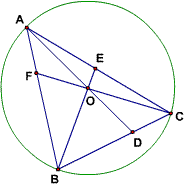
\includegraphics[scale=0.8]{extcircum}
\end{center}

\textit{Has hints.}
\begin{sketch}
    \begin{enumerate}
        \item Construct a perpendicular from A to BC.
        \item Express various ratios in terms of trigonometric functions.
    \end{enumerate}
\end{sketch}

\begin{mdsoln}
    Since $AO=BO=CO=R$, what we want to prove is equivalent to$$\frac{AO}{AD}+\frac{BO}{BE}+\frac{CO}{CF}=2$$But we know that$$\frac{AO}{AD}=\frac{[ACOB]}{[ABC]}$$and similar expressions for $BO/BE$ and $CO/CF$. So$$\frac{AO}{AD}+\frac{BO}{BE}+\frac{CO}{CF}=\frac{[ACOB]+[BAOC]+[CBOA]}{ABC}=2$$as desired.
\end{mdsoln}


\subsection{Problem 2}
Given the following information about a triangle: the radius $R$ of its circumscribed circle, the length $c$ of one of its sides, and the ratio $\dfrac ab$ of the other two sides; determine all three sides and angles of the triangle.

\textit{Has hints.}
\begin{sketch}
    \begin{enumerate}
        \item Use the Law of Sines. (This is good advice in general when you know the circumradius.)
        \item Draw a perpendicular from $C$ to $AB$.
    \end{enumerate}
\end{sketch}

\begin{mdsoln}
    There are actually two possibilities for the triangle: one with $\angle C\ge 90^\circ$ and one with $\angle C\le 90^\circ$ (unless $C=90^\circ$, in which case there is only one possibility). We will find both of these solutions.

    Draw segment $AB$ of length $c$.
    
    We first try to find $D$ on segment $AB$ such that $DB/DA=a/b$ (why we want this will become clear later on). Supposing that we were given $a/b$ as the ratio of some two lengths $x$ and $y$, we can find $D$ in the following manner: Construct a line parallel to and distinct from $AB$ and choose points $X,Y,Z$ on the line such that $XY=x$, $YZ=y$, and $Y$ lies on segment $XZ$. Then, find the intersection $P$ of $XB$ and $ZA$. There is a homothety centered at $P$ taking $X,Y,Z$ to $B,D,A$, respectively, since $BD/DA=XY/YZ$. The desired point $D$ must therefore be the intersection of $PY$ and $AB$.
    
    Now, by the Law of Sines, $\sin \angle C=c/2R$. We construct a circle with diameter $ST$ of length $2R$, and find an intersection point $U$ of the circle with the circle of radius $c$ centered at $S$. It is clear that $\triangle STU$ has a right angle at $U$, that $ST=2R$ and $SU=c$. Hence, $\angle T$ must be equal to angle $\angle C$ or else to $180^\circ-\angle C$. These two possible values for $\angle C$ give us the two solutions to the problem.
    
    For each of the values of $\angle C$, we proceed as follows:
    
    Now we construct points $E,F$ on the same side of line $AB$ such that $AE=DE$, $DF=BF$, and $\angle DEA=\angle BFD=\angle C/2$. The circumcircles of $\triangle ADE$ and $\triangle DBF$ must intersect at some point $Q$ such that $\angle DQA=\angle BQD=\angle C/2$. Hence, $\angle BQA=\angle C$. Moreover, since $QD$ is the angle bisector of $\angle BQA$, the Angle-Bisector Theorem implies that $QB/QA=DB/DA=a/b$. Hence, $Q$ satisfies all the requirements for our desired point $C$.
    
    It is simple to work through this logic to show that our solution does indeed produce all possible solutions to the problem.        
\end{mdsoln}




\subsection{Problem 3}
Show that if $A$, $B$, $C$ are angles of a triangle, then
\[
\sin \dfrac A2 \sin \dfrac B2 \sin \dfrac C2 \leq \dfrac 18.
\]

\begin{mdsoln}
    We proved in class that$$\sin \dfrac A2=\sqrt{\frac{(s-b)(s-c)}{bc}}$$Using this and similar expressions for $\sin (B/2)$ and $\sin (C/2)$, we get\begin{eqnarray*}\sin \dfrac A2 \sin \dfrac B2 \sin \dfrac C2&=&\sqrt {\frac {(s - b)(s - c)}{bc}} \cdot \sqrt {(\frac {(s - c)(s - a)}{ca}} \cdot \sqrt {\frac {(s - a)(s - b)}{ab}}\\ &=& \frac{(s-a)(s-b)(s-c)}{abc}\\ &=&\frac{s(s-a)(s-b)(s-c)}{sabc}\\ &=&\frac{A^2}{sabc}\\ &=&\frac{\frac{abc}{4R}\cdot rs}{sabc}\\ &=&\frac{r}{4R}\\ &\le &\frac{1}{8}\end{eqnarray*}where the last step follows from Euler’s Inequality $R\ge 2r$.
\end{mdsoln}



\subsection{Problem 4}
In triangle $ABC$, prove that there is a point $D$ on side $AB$ such that $CD$ is the geometric mean of $AD$ and $DB$ if and only if
\[
\sin A \cdot \sin B \leq \sin^2 \dfrac C2 .
\]



\textit{Has hints.}
\begin{sketch}
    \begin{enumerate}
        \item Extend $CD$ to the circumcircle of $ABC$.
        \item Use power of a point.
        \item Look for extreme cases.
    \end{enumerate}
\end{sketch}

\begin{mdsoln}
    Suppose that $D$ is just a variable point on side $AB$. Let $P$ be the other intersection of ray $CD$ with the circumcircle $\omega$ of $\triangle ABC$. By Power of a Point, $AD\cdot DB=CD\cdot DP$. Observe that $CD$ is the geometric mean of $AD$ and $DB$ if and only if$$CD^2=AD\cdot DB=CD\cdot DP$$which is the case if and only if $CD=DP$.

    So it suffices to consider whether there exists a $D$ for which $CD=DP$. Consider, for $D$ varying along segment $AB$, the locus $L$ of points $Q$ such that $Q$ is on ray $CD$ with $CD=DQ$. There exists a $D$ such that $CD=DP$ if and only if $L$ intersects $\omega$. Note that $L$ is merely the image of segment $AB$ under a homothety of ratio 2 centered at $C$. $L$ intersects $\omega$ if and only if the tangent line $\ell$ to $\omega$ which is parallel to $AB$ and on the opposite side of it from point $C$ is the image of line $AB$ under a homothety of ratio greater than or equal to 2.
    
    Suppose that $\ell$ is tangent to $\omega$ at $X$. Since $\ell\parallel AB$, $X$ must bisect the arc $AB$, so $CX$ must bisect angle $C$. Let $CX$ meet $AB$ at $Y$. Then, the homothety centered at $C$ taking line $AB$ to $\ell$ has ratio $CX/CY$. Therefore, a $D$ of the desired form exists if and only if $CX/CY\ge 2$, which is equivalent to\begin{eqnarray*}1&\le & \frac{XY}{CY}\\ &=&\frac{XY}{AY}\cdot \frac{AY}{CY}\\ &=&\frac{\sin \angle YAX}{\sin \angle AXY}\cdot \frac{\sin \angle YCA}{\sin \angle CAY}\\ &=&\frac{\sin \angle BCY}{\sin \angle ABC}\cdot \frac{\sin \angle YCA}{\sin \angle CAB}\\ &=&\frac{\sin^2 (C/2)}{\sin B\sin A}\end{eqnarray*}which gives us the desired result.        
\end{mdsoln}





\subsection{Problem 5}
$ABC$ is a triangle. The tangent to the circumcircle at $A$ meets the line $BC$ at $D$. The perpendicular to $BC$ at $B$ meets the perpendicular bisector of $AB$ at $E$, and the perpendicular to BC at C meets the perpendicular bisector of AC at F. Show that D, E, F are collinear.

% https://s3.amazonaws.com/classroom.artofproblemsolving.com/Classes/GeomOlympiad/Images/collfeet.gif
\begin{center}
    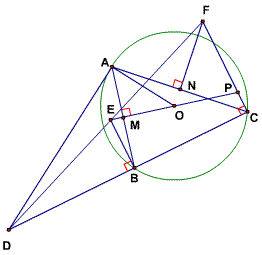
\includegraphics[scale=0.8]{collfeet}
\end{center}

\begin{mdsoln}
    We see that\begin{eqnarray*}FC&=&\frac{\dfrac{1}{2}AC}{\cos(90-\angle C)}\\ EB&=&\frac{\dfrac{1}{2}AB}{\cos(90-\angle B)}\end{eqnarray*}Hence,\begin{eqnarray*}\frac{EB}{FC}&=&\frac{\cos(90-\angle C)}{\cos(90-\angle B)}\cdot \frac{AB}{AC}\\ &=&\frac{\sin\angle C}{\sin\angle B}\cdot \frac{AB}{AC}\\ &=&\frac{\sin\angle BAD}{\sin\angle DBA}\cdot \frac{AB}{AC}\\ &=&\frac{BD}{AD}\cdot \frac{AB}{AC}\\ &=&\frac{BD}{AD\cdot \dfrac{AC}{AB}}\\ &=&\frac{BD}{CD}\end{eqnarray*}where the last step follows from $\triangle ABD\sim \triangle CAD$. Since $EB/FC=BD/CD$, points $D,E,F$ must be collinear, as desired.    
\end{mdsoln}



\subsection{Problem 6}
Given the triangle $ABC$, let $D, E, F$ be the midpoints of $BC, AC, AB$ respectively and $G$ be the centroid of $ABC$. For each value of angle $BAC$, how many non-similar triangles are there in which $AEGF$ is a cyclic quadrilateral.

% https://s3.amazonaws.com/classroom.artofproblemsolving.com/Classes/GeomOlympiad/Images/centro.gif
\begin{center}
    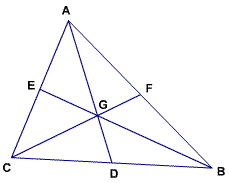
\includegraphics[scale=0.8]{centro}
\end{center}

\begin{mdsoln}
    Fix $\angle BAC$ at some value $\theta$ and fix $BC$ at some value $a$. Clearly, if $AEGF$ is cyclic, then $\angle BGC=180^\circ-\angle BAC$, implying that we need only consider $\theta\le 90^\circ$ (since for $\theta>90^\circ$, angles $BGC$ and $BAC$ are both greater than $90^\circ$, so $AEGF$ cannot be cyclic).

    Observe that $AEGF$ is cyclic implies that $\angle GAE=\angle GFE=\angle GCB$. This implies $\triangle DGC\sim \triangle DCA$, which is in turn implies $CD^2=(DG)(DA)=3DG^2$. Since $CD=a/2$, this means that$$DG=\frac{\sqrt{3}a}{6}$$As previously noted, $AEGF$ cyclic also implies $\angle BGC=180^\circ-\theta$. Hence, $AEGF$ can be cyclic only if (but not necessarily if) both $DG=\dfrac{\sqrt{3}a}{6}$ and $\angle BGC=180^\circ-\theta$. We will now consider how many triangles $BGC$ exist that satisfy both these requirements.
    
    Consider the arc which is the locus of points $G$ such that $\angle BGC=180^\circ-\theta$. The length $GD$ from $G$ to the midpoint $D$ of $BC$ varies from a minimum where $G$ is at the midpoint of the arc (where $GD=(a/2)\cot (\angle BGC/2)=(a/2)\tan(\theta/2)$) to a maximum where $G$ is at either $B$ or $C$ (where $GD=a/2$). The length $GD$ varies continuously between these two extremes. We seek $GD=\frac{\sqrt{3}a}{6}$. If$$\frac{a}{2}\tan(\theta/2)\le \frac{\sqrt{3}a}{6}\le \frac{a}{2}$$then there is either exactly one or exactly two points on the arc with $GD$ as desired (if there are two spots then they yield exactly the same triangle $GBC$, merely reflected about the perpendicular bisector of $BC$). If the inequality above does not hold, then there is no location of $G$ that works, so there are no triangles $ABC$ such that $AEGF$ is cyclic.
    
    We now consider when the inequality holds. Notice that the statement$$\frac{\sqrt{3}a}{6}\le \frac{a}{2}$$is true, and the statement$$\frac{a}{2}\tan(\theta/2)\le =\frac{\sqrt{3}a}{6}$$is true if and only if$$\theta\le 2\tan^{-1}(\frac{\sqrt{3}}{3})=60^\circ$$
    For $\theta\le 60^\circ$, then, there is exactly one triangle $BGC$ that satisfies $DG=\dfrac{\sqrt{3}a}{6}$ and $\angle BGC=180^\circ-\theta$. Letting $A$ be on ray $DG$ such that $DA=3DG$, we see that $G$ must be the centroid of $\triangle ABC$ and that $DG=\dfrac{\sqrt{3}a}{6}$ implies that $\triangle DGC\sim \triangle DCA$ (by our previous logic), so that, if $E$ and $F$ are the midpoints of $AC$ and $AB$, respectively, $\angle GAE=\angle GCB=\angle GFE$. We conclude that $AEGF$ is cyclic and hence that $\angle BAC=180^\circ-\angle BGC=\theta$, so $\triangle ABC$ is a triangle of the desired form.
    
    We conclude that, for $\theta\le 60^\circ$, there is exactly one solution to the problem, and otherwise there are no solutions.    
\end{mdsoln}









\chapter{Inversion}
\section{Lesson Transcript}
%-- Message Achilleas ( moderator )
% Hi, everyone!

%------------------
%-- Message MTHJJS ( user )
% Hi!

%------------------
%-- Message MeepMurp5 ( user )
% Hi

%------------------
%-- Message bryanguo ( user )
% Hi!

%------------------
%-- Message pritiks ( user )
% hello!

%------------------
%-- Message mark888 ( user )
% Hi!

%------------------
%-- Message leoouyang ( user )
% hello

%------------------
%-- Message ca981 ( user )
% Hi!

%------------------
%-- Message Achilleas ( moderator )
% \textbf{Olympiad GeometryWeek 12: Inversion}

%------------------
%-- Message Achilleas ( moderator )
% As this is the last class, don't forget to fill out your feedback form on the class homepage! Your ideas and suggestions help us make AoPS even more amazing than it already is.

%------------------
%-- Message Achilleas ( moderator )
In our first 11 classes we discussed tactics and approaches which, while not always completely straightforward, can be demystified by a little experience.  Many of them were intuitively clear (though the problems we worked might still be quite challenging).

%------------------
%-- Message Achilleas ( moderator )
Above all, there wasn't anything magical about our tools - we could see them and understand them pretty well, and it didn't require any great leaps of faith or genius to use them.

%------------------
%-- Message Achilleas ( moderator )
For example, the geometric transformations we've discussed - dilation (homothety), reflection, rotation - we have a physical feel for.

%------------------
%-- Message Achilleas ( moderator )
Today, we take a step outside that nice safe realm and into an area that might feel a little like magic at first.

%------------------
%-- Message Achilleas ( moderator )
Today, we talk about the \textbf{geometric transformation inversion}.

%------------------
%-- Message Achilleas ( moderator )
Inversion, as you'll see, is fairly limited in the problems it can be applied to, but when it's useful it usually blows apart a problem pretty quickly.

%------------------
%-- Message Achilleas ( moderator )
The statement of inversion is pretty simple.  In reflection, we reflect over a line.  In inversion, we `reflect' over a circle.

%------------------
%-- Message Achilleas ( moderator )
\begin{definition}
Specifically, if we have a circle with center $O$ and radius $r$, the image of point $P$ upon inversion about the circle is the point $P'$ on ray $OP$ such that $OP\cdot OP' = r^2$.    
\end{definition}

%------------------
%-- Message Achilleas ( moderator )



\begin{center}
\begin{asy}
import cse5;
import olympiad;
// unitsize(4cm);

size(250);
pen s = fontsize(8);

/* helper functions */
path scale(real s, pair D, pair E, real p) { return (point(D--E,p)+scale(s)*(-point(D--E,p)+D)--point(D--E,p)+scale(s)*(-point(D--E,p)+E));}
pair r(pair A, pair B, real d){return B+rotate(d)*(A-B);}

real t = .4;
pair O = origin, X = dir(0), P = point(O--X,t), PP = scale(1/(t))*X;
draw(Circle(O,1),heavygreen);
draw(O--scale(1.1)*PP);
dot(MP("O",O,S,s)^^MP("P",P,S,s)^^MP("X",X,SE,s)^^MP("P'",PP,S,s));
draw(brace(shift((0,.05))*O, shift((0,.05))*X)^^MP("r",point(O--X,.5),6N,s));

\end{asy}
\end{center}





%------------------
%-- Message Achilleas ( moderator )
What is the inverse of P' with respect to the circle?

%------------------
%-- Message RP3.1415 ( user )
% $P$

%------------------
%-- Message Ezraft ( user )
% $P$

%------------------
%-- Message Gamingfreddy ( user )
% P

%------------------
%-- Message Yufanwang ( user )
% P

%------------------
%-- Message ca981 ( user )
% P

%------------------
%-- Message mark888 ( user )
% P

%------------------
%-- Message coolbluealan ( user )
% P

%------------------
%-- Message sae123 ( user )
% P

%------------------
%-- Message mustwin_az ( user )
% P

%------------------
%-- Message bryanguo ( user )
% P

%------------------
%-- Message Trollface60 ( user )
% P

%------------------
%-- Message J4wbr34k3r ( user )
% P

%------------------
%-- Message MeepMurp5 ( user )
% P

%------------------
%-- Message MathJams ( user )
% P

%------------------
%-- Message Achilleas ( moderator )
We know that point $P$ is on ray $OP'$ and that $OP \cdot OP' = r^2$, so $P$ is the inverse of $P'$.  Hence, like reflection and 180-degree rotations, the transformation inversion has a period of 2 (which means that if we apply it twice, everything is back where it started in the end).

%------------------
%-- Message Achilleas ( moderator )
\vspace{6pt}
When we work with a transformation (like homothety, reflection, rotation, and now inversion), what are some easy questions we can ask that will help us understand our transformation?

%------------------
%-- Message sae123 ( user )
% are angles or lengths preserved?

%------------------
%-- Message dxs2016 ( user )
% are lengths/angles preserved

%------------------
%-- Message pritiks ( user )
% where does the transformation map the points/lines?

%------------------
%-- Message MTHJJS ( user )
% 1. keep distance or not?  2. What happens with whole shapes?

%------------------
%-- Message JacobGallager1 ( user )
% What angles does it preserve?

%------------------
%-- Message Yufanwang ( user )
% Is a shape always mapped to a similar shape?

%------------------
%-- Message MathJams ( user )
% where does circles/lines go under inversion?

%------------------
%-- Message Ezraft ( user )
% Is there an identity (a point which the inversion maps to itself)

%------------------
%-- Message Achilleas ( moderator )
1. We can figure out what points are fixed under the transformation. 


2. We can figure out what figures (lines, circles, etc) are fixed.


3. We can think about how to construct the image of a point.


4. We can think about what happens when we transform figures like circles and lines.


5. We can think about what quantities remain constant under the transformation.

%------------------
%-- Message Achilleas ( moderator )
\begin{remark}
Notice that most of these involve figuring what remains the same under the transformation - this is where much of the usefulness of any sort of transformation (even transformations outside geometry, such as algebraic transformations) comes from.  Understanding what remains fixed is often the key to understanding the transformation.    
\end{remark}

%------------------
%-- Message Achilleas ( moderator )
So, we'll start with points.  What points are fixed?  (In other words, for what points P is the inverse of P also P?)

%------------------
%-- Message MeepMurp5 ( user )
% points on the circle

%------------------
%-- Message coolbluealan ( user )
% points on the circle

%------------------
%-- Message J4wbr34k3r ( user )
% Any point on the original circle.

%------------------
%-- Message Gamingfreddy ( user )
% All points on the circle

%------------------
%-- Message JacobGallager1 ( user )
% Points on the circle

%------------------
%-- Message mark888 ( user )
% points on the circle

%------------------
%-- Message SlurpBurp ( user )
% points on the circle

%------------------
%-- Message Wangminqi1 ( user )
% When $P$ is on the circle

%------------------
%-- Message Riya_Tapas ( user )
% When $P$ lies on the circle

%------------------
%-- Message Ezraft ( user )
% all points on the circle

%------------------
%-- Message pike65_er ( user )
% If P lies on the circle

%------------------
%-- Message mustwin_az ( user )
% If P is on circle O

%------------------
%-- Message Achilleas ( moderator )
Only points on the circle map to themselves.  The inverse of a point inside the circle is outside the circle and vice versa (we can see this from $OP \cdot OP' = r^2$: if $OP < r$, then $OP'$ must be greater than $r$ and vice versa).

%------------------
%-- Message Achilleas ( moderator )
What point should we be curious about at this point?

%------------------
%-- Message vsar0406 ( user )
% Point O

%------------------
%-- Message SlurpBurp ( user )
% the center of the circle

%------------------
%-- Message pike65_er ( user )
% the center of the circle

%------------------
%-- Message JacobGallager1 ( user )
% The center of the circle

%------------------
%-- Message MathJams ( user )
% Where does O go?

%------------------
%-- Message sae123 ( user )
% oh where does the center get mapped?

%------------------
%-- Message Achilleas ( moderator )
The center of the circle - what is its inverse?

%------------------
%-- Message MathJams ( user )
% O goes to $P_{\infty}$

%------------------
%-- Message J4wbr34k3r ( user )
% The point at infinity.

%------------------
%-- Message Achilleas ( moderator )
Since OP = 0 when P is the center of the circle, there is no point P' such that $OP \cdot OP' = r^2$.  To get around this, we say that the inverse of the center of the circle is ``the point at infinity", since as P gets closer and closer to O, its inverse gets farther and farther away.  Conversely, the inverse of the ``point at infinity" is the center of our circle.

%------------------
%-- Message Achilleas ( moderator )
You may have heard before that we can add a ``line at infinity" to the Euclidean plane, to obtain the so called real projective plane. That is not what we are doing here. We now add a single ``point at infinity" to the plane. To do this, identify the Euclidean plane to the complex numbers, then add the ``point at infinity" to obtain the so called inversive plane. The inversive plane is also called the complex projective line.

%------------------
%-- Message Achilleas ( moderator )
One way to visualize this is to identify the inversive plane to the Riemann sphere. Imagine that you bend the plane to form a sphere, such that all ends meet at the North Pole of the sphere, which we denote $\infty$. The lines from our plane bend to become circles on the sphere, passing through $\infty$.

%------------------
%-- Message Achilleas ( moderator )
There is a one-to-one map $P$ between the Riemann sphere and the inversive plane, called the stereographic projection. $P(A)$ is just the intersection of the line through $\infty$ and $A$ with our plane. We have $P(\infty)=\infty$. Note that the circles through $\infty$ become lines in the plane.

%------------------
%-- Message Achilleas ( moderator )
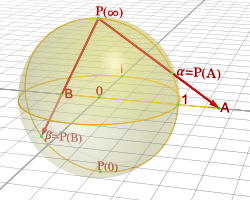
\includegraphics[]{778a917377fe8c15e4e748da260bc93f2bc63e73}
% //cdn.artofproblemsolving.com/images/7/7/8/778a917377fe8c15e4e748da260bc93f2bc63e73.png ]]]

%------------------
%-- Message Achilleas ( moderator )
This means that we can think of lines in the plane as infinite circles (circles through $\infty$ on the Riemann sphere). More on this later.

%------------------
%-- Message Achilleas ( moderator )
What figures are fixed (i.e. what lines/circles/etc map to themselves, even if points on that figure do not map to themselves)?

%------------------
%-- Message bryanguo ( user )
% the circle we perform inversion on is fixed

%------------------
%-- Message Achilleas ( moderator )
Clearly the circle we are inverting about maps to itself, as every point on it maps to itself.

%------------------
%-- Message Achilleas ( moderator )
Are there any other fixed figures?

%------------------
%-- Message Gamingfreddy ( user )
% Lines through the center of the circle

%------------------
%-- Message MathJams ( user )
% Any line through O is fixed

%------------------
%-- Message sae123 ( user )
% any line through the center of the circle maps to itself

%------------------
%-- Message JacobGallager1 ( user )
% Lines through $O$?

%------------------
%-- Message RP3.1415 ( user )
% a line through the center of the circle

%------------------
%-- Message Achilleas ( moderator )
Lines through O (the center of inversion) are fixed.  Make sure you see this.

%------------------
%-- Message Achilleas ( moderator )
There is one more set of non-obvious (but very important) fixed figures.  We'll come back to it soon.

%------------------
%-- Message Achilleas ( moderator )
Next we'll talk about construction.  Thinking about how to construct the diagram for a given problem can help us figure out how to solve the problem (I've solved a surprising number of problems this way).  Similarly, thinking about how to construct the image of a transformation can help us understand the transformation.

%------------------
%-- Message Achilleas ( moderator )
Suppose point P is inside circle with center O.  How do we construct the inverse of P about O?  (Call the inverse P' as usual.)

%------------------
%-- Message Achilleas ( moderator )
What information do we have?

%------------------
%-- Message MathJams ( user )
% $OP\cdot OP' = r^2$

%------------------
%-- Message AOPS81619 ( user )
% $OP\cdot OP'=r^2$

%------------------
%-- Message Trollface60 ( user )
% OP * OP' = r^2

%------------------
%-- Message Achilleas ( moderator )
What else?

%------------------
%-- Message JacobGallager1 ( user )
% $P'$ is on the line $OP$

%------------------
%-- Message pike65_er ( user )
% we know P' lies on line OP

%------------------
%-- Message MeepMurp5 ( user )
% $O, P, P'$ are collinear

%------------------
%-- Message sae123 ( user )
% $O,P,P'$ are collinear

%------------------
%-- Message mustwin_az ( user )
% O,P,P' collinear

%------------------
%-- Message vsar0406 ( user )
% O, P, and P' are collinear

%------------------
%-- Message Catherineyaya ( user )
% $P'$ lies on ray $OP$

%------------------
%-- Message RP3.1415 ( user )
% O, P, P' are collinear

%------------------
%-- Message Achilleas ( moderator )
We know that point P' lives on ray OP, and that $OP \cdot OP' = OX^2$:

%------------------
%-- Message Achilleas ( moderator )
% https://s3.amazonaws.com/classroom.artofproblemsolving.com/Classes/GeomOlympiad/Images/inversion.gif
\begin{center}
    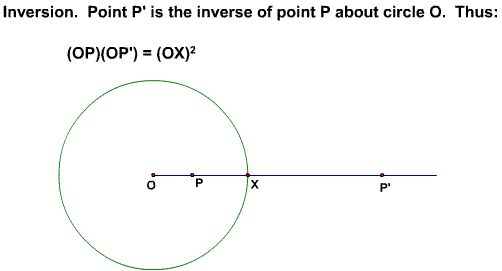
\includegraphics[scale=0.8]{inversion}    
\end{center}
%------------------
%-- Message Achilleas ( moderator )
So we can start our construction by drawing ray OP.  Now we have to find P'.  What tools are we likely to use?

%------------------
%-- Message leoouyang ( user )
% Power of Point

%------------------
%-- Message sae123 ( user )
% Kind of reminds me of power of a point

%------------------
%-- Message SlurpBurp ( user )
% similar triangles?

%------------------
%-- Message MTHJJS ( user )
% similarity

%------------------
%-- Message Ezraft ( user )
% power of a point

%------------------
%-- Message xyab ( user )
% power of a point?

%------------------
%-- Message MathJams ( user )
% Power of a point

%------------------
%-- Message Achilleas ( moderator )
We seek the point P' such that $OP \cdot OP' = OX^2$.  The obvious candidates are power of a point and similar triangles.

%------------------
%-- Message Achilleas ( moderator )
If we try power of a point, we'll want to draw a circle passing through P and P', and we'll want the tangent from O to hit that circle somewhere on the green circle.  But given only P (not P' ), it's not clear how we construct this circle.

%------------------
%-- Message Achilleas ( moderator )
So we turn to similar triangles.  But what's the problem with that?

%------------------
%-- Message Trollyjones ( user )
% there are no triangles to work with

%------------------
%-- Message Trollface60 ( user )
% no triangles

%------------------
%-- Message Gamingfreddy ( user )
% We don't have triangles

%------------------
%-- Message sae123 ( user )
% no triangles!

%------------------
%-- Message MathJams ( user )
% We don't have any triangles!

%------------------
%-- Message MeepMurp5 ( user )
% there aren't any, so we need to make them

%------------------
%-- Message mustwin_az ( user )
% No triangles or angles

%------------------
%-- Message smileapple ( user )
% we don't have any triangles

%------------------
%-- Message Catherineyaya ( user )
% there are no triangles

%------------------
%-- Message xyab ( user )
% we dont have triangles

%------------------
%-- Message Achilleas ( moderator )
No triangles.

%------------------
%-- Message Achilleas ( moderator )
Hmm. . .  So we think maybe we should build triangles.  What kind of triangles should we think of building?

%------------------
%-- Message Gamingfreddy ( user )
% Right triangles

%------------------
%-- Message MeepMurp5 ( user )
% probably right triangles

%------------------
%-- Message dxs2016 ( user )
% right triangles?

%------------------
%-- Message xyab ( user )
% right triangles

%------------------
%-- Message ca981 ( user )
% right triangle

%------------------
%-- Message Trollyjones ( user )
% right triangles

%------------------
%-- Message Achilleas ( moderator )
We think to try building right triangles since they often give us similar triangles.  Right triangles.  Circle.  Point outside the circle.  Does anyone want to take a guess at how to construct P' now?

%------------------
%-- Message J4wbr34k3r ( user )
% The tangents from P' to the circle intersect it at the points the line passing through P and perpendicular to OP intersect the circle.

%------------------
%-- Message Achilleas ( moderator )
We think `Right triangles.  Circle.  Point outside the circle.  Let's draw tangents.  We need to incorporate P somehow, so maybe P is the intersection of OP' and the segment connecting the points of tangency when we draw the tangents through P'

%------------------
%-- Message MathJams ( user )
% Construct a line perpendicular to $OX$ through $P$ and let it intersect the circle at $A$ and $B$, and construct $P'$ by extending a line tangent to the circle at A and finding it's intersection with ray $OX$

%------------------
%-- Message Achilleas ( moderator )
Are we right?  Is P' the intersection of ray OP and the tangent to the circle at point A as shown in the diagram?

%------------------
%-- Message Achilleas ( moderator )



\begin{center}
\begin{asy}
import cse5;
import olympiad;
// unitsize(4cm);

size(250);
pen s = fontsize(8);

/* helper functions */
path scale(real s, pair D, pair E, real p) { return (point(D--E,p)+scale(s)*(-point(D--E,p)+D)--point(D--E,p)+scale(s)*(-point(D--E,p)+E));}
pair r(pair A, pair B, real d){return B+rotate(d)*(A-B);}

real t = .4;
pair O = origin, X = dir(0), P = point(O--X,t), PP = scale(1/(t))*X;
pair A = tangent(PP,O,1,1), B = tangent(PP,O,1,2);

draw(Circle(O,1),heavygreen);
draw(O--scale(1.1)*PP);
dot(MP("O",O,S,s)^^MP("P",P,SE,s)^^MP("X",X,SE,s)^^MP("P'",PP,S,s));
draw(O--MP("A",A,N,s)--PP--MP("B",B,S,s)--cycle^^A--B);
draw(rightanglemark(O,A,PP,3)^^rightanglemark(O,P,A,3)^^rightanglemark(O,B,PP,3),heavyred);

\end{asy}
\end{center}





%------------------
%-- Message pritiks ( user )
% yes

%------------------
%-- Message Achilleas ( moderator )
Why?

%------------------
%-- Message Achilleas ( moderator )
How do we know that $OP\cdot OP'=OX^2$ in the above figure?

%------------------
%-- Message smileapple ( user )
% similar triangles $\triangle OPA\sim\triangle OAP'$

%------------------
%-- Message Lucky0123 ( user )
% Because due to similar triangles $\triangle POB$ and $\triangle PBP',$ we know that $OP * OP' = OX^2$

%------------------
%-- Message MathJams ( user )
% Because $\triangle OAP\sim \triangle OP'A \implies \frac{OA}{OP}=\frac{OP'}{OA}\implies OA^2=OP\cdot OP'=OX^2$

%------------------
%-- Message Catherineyaya ( user )
% $\triangle APO\sim\triangle P'AO$ so $OP/AO=AO/OP'$ and $OP\cdot OP'=OA^2=OX^2$

%------------------
%-- Message ca981 ( user )
% triangle AOP and P'OA are similar

%------------------
%-- Message coolbluealan ( user )
% $\triangle OPA \sim \triangle OAP'$

%------------------
%-- Message JacobGallager1 ( user )
% $\triangle OPA \sim \triangle APP' \sim \triangle OAP'$, so $\frac{OP}{OX} = \frac{OX}{OP'}$

%------------------
%-- Message Gamingfreddy ( user )
% Triangles OAP and OP'A are similar, so OP/AO = AO/OP' -> OP * OP' = (OX)^2 since AO = OX

%------------------
%-- Message Ezraft ( user )
% because $\triangle OPA \sim \triangle OAP',$ $\frac{OP}{OA} = \frac{OA}{OP'}$ and since $OA = OX,$ we see that $OP \cdot OP' = OX^2$

%------------------
%-- Message Achilleas ( moderator )
Since $\triangle OAP \sim \triangle OP'A$, we have $\dfrac{OP'}{OA} = \dfrac{OA}{OP}$, or $OP \cdot OP' = OA^2$.  $OA$ is a radius, so we have our desired relationship.  $P'$ is the intersection of ray $OP$ and the tangent to the circle at point $A$ as shown in the diagram.  How do we do our construction starting from the original $P$?

%------------------
%-- Message MathJams ( user )
% We can construct a line perpendicular to $OX$ through $P$ and let it intersect the circle at $A$ and $B$, and construct $P'$ by extending a line tangent to the circle at A and finding it's intersection with ray $OX$

%------------------
%-- Message Achilleas ( moderator )
We simply draw a line perpendicular to OP through P to get A.  Then draw OA, and a line through A perpendicular to OA.  Where this line meets ray OP is our P'.

%------------------
%-- Message Achilleas ( moderator )
Once again, we're seeing that similar triangles are at the heart of one of our powerful geometric tools.

%------------------
%-- Message Achilleas ( moderator )
Next let's talk about what happens when we invert lines and circles.  We already know what happens if we invert the circle we are inverting about - we get that circle back.  We also know that if we invert a line through the center we get that line back.

%------------------
%-- Message Achilleas ( moderator )
What happens if we invert a circle with center O but a different radius?  (Say this circle has radius s and our original circle that we are inverting about has radius r, as usual.)

%------------------
%-- Message coolbluealan ( user )
% we get a circle with center O and radius r^2/s

%------------------
%-- Message J4wbr34k3r ( user )
% A circle with center O and radius $\frac{r^{2}}{s}$

%------------------
%-- Message Gamingfreddy ( user )
% We get a circle with center O and radius r^2/s

%------------------
%-- Message MeepMurp5 ( user )
% circle centered at $O$ with radius $r^2/s$

%------------------
%-- Message dxs2016 ( user )
% OP*OP' = s^2 --> OP' = s^2/OP. if P is point on circumference of circle, length of OP' is fixed --> circle

%------------------
%-- Message pike65_er ( user )
% a circle with radius $\frac{r^2}{s}$ centered at O

%------------------
%-- Message ca981 ( user )
% Another concentric circle with radius = r^2/s

%------------------
%-- Message Achilleas ( moderator )
Every point on the inverse of the circle with radius s will be a distance of $r^2/s$ away from O, since $OP \cdot OP' = r^2$ and $OP = s$ for all points $P$ on the circle with radius $s$.

%------------------
%-- Message Achilleas ( moderator )
Conversely, every point on our inverse circle can be produced by inverting our original circle.

%------------------
%-- Message Achilleas ( moderator )
Hence, our inverse is a circle with radius $r^2/s$.

%------------------
%-- Message Achilleas ( moderator )
Let's try lines that don't pass through the center.  We'll start with one that doesn't even touch the circle:

%------------------
%-- Message Achilleas ( moderator )



\begin{center}
\begin{asy}
import cse5;
import olympiad;
// unitsize(4cm);

pair O, SS, SSP;
O = (0,0);
SS = (1.7,0);
SSP = (1/1.7,0);
unitsize(0.5inch);
defaultpen(black+0.75);
draw(Circle((0,0),1));
draw((1.7,-1.2)--(1.7,2));

\end{asy}
\end{center}





%------------------
%-- Message Achilleas ( moderator )
Any observations?

%------------------
%-- Message J4wbr34k3r ( user )
% A circle passing through O but always inside the original circle.

%------------------
%-- Message MathJams ( user )
% all the points on the line invert to points inside the circle

%------------------
%-- Message JacobGallager1 ( user )
% The image of the line must lie entirely within the circle

%------------------
%-- Message SlurpBurp ( user )
% the image must pass through the center of the circle, because the line contains the point at infinity

%------------------
%-- Message bryanguo ( user )
% if we invert points on that line wrt the circle the points that have been inverted will be inside the circle

%------------------
%-- Message Achilleas ( moderator )
If we invert this line, we know that points arbitrarily close to the center will be in the image, as the line goes infinitely far away from the circle (so the images of those very, very far away points will be very, very close to the center).

%------------------
%-- Message Achilleas ( moderator )
What point on the line will have an image that is farthest from the center of inversion?

%------------------
%-- Message J4wbr34k3r ( user )
% The image of the center when projected onto the line.

%------------------
%-- Message smileapple ( user )
% the projection of the center onto the line

%------------------
%-- Message coolbluealan ( user )
% The point closest to the circle

%------------------
%-- Message dxs2016 ( user )
% the point H where OH is perpendicular to the line

%------------------
%-- Message bryanguo ( user )
% the point on the line which is the foot from the center of the circle to the line

%------------------
%-- Message AOPS81619 ( user )
% The closest point to the circle

%------------------
%-- Message Ezraft ( user )
% the point closest to the circle

%------------------
%-- Message Catherineyaya ( user )
% the point closest to the center

%------------------
%-- Message Wangminqi1 ( user )
% The point on the perpendicular line from the center of the circle

%------------------
%-- Message MathJams ( user )
% the point closest to the circle, or the foot of the perpendicular from the center to the line

%------------------
%-- Message Achilleas ( moderator )
The point that is the inverse of the point on the line closest to the center will be farthest from the center in the image of the line.  This point is the image of the foot of the perpendicular from the center of the circle to the line:

%------------------
%-- Message Achilleas ( moderator )



\begin{center}
\begin{asy}
import cse5;
import olympiad;
// unitsize(4cm);

pair O, SS, SSP;
O = (0,0);
SS = (1.7,0);
SSP = (1/1.7,0);
unitsize(0.5inch);
defaultpen(black+0.75);
draw(Circle((0,0),1));
draw((1.7,-1.2)--(1.7,2));
draw(O--SS);
dot(O,p=black+3);
dot(SSP,p=black+3);
label("$O$",O,S);
label("$S'$",SSP,S);
label("$S$",SS,E);
draw(rightanglemark((1.7,1),SS,O,s=5));

\end{asy}
\end{center}





%------------------
%-- Message Achilleas ( moderator )
Now what?

%------------------
%-- Message MathJams ( user )
% consider another arbitrary point on the line

%------------------
%-- Message dxs2016 ( user )
% try some more points?

%------------------
%-- Message Achilleas ( moderator )
The images of points above S will be above segment OS' and get gradually closer to O.  Those below S will have images below segment OS' and these images will be gradually closer to O.  What might we guess the image of our line is?

%------------------
%-- Message MathJams ( user )
% a circle

%------------------
%-- Message coolbluealan ( user )
% circle

%------------------
%-- Message AOPS81619 ( user )
% A circle

%------------------
%-- Message bryanguo ( user )
% image of our line is a circle

%------------------
%-- Message dxs2016 ( user )
% circle?

%------------------
%-- Message pike65_er ( user )
% a circle

%------------------
%-- Message Achilleas ( moderator )
Inversion seems all about circles and our image is clearly not a line, so we guess that the image is a circle. Which circle it is? Can we be more specific?

%------------------
%-- Message Wangminqi1 ( user )
% The circle with diameter $OS'$

%------------------
%-- Message Gamingfreddy ( user )
% The circle with diameter OS'

%------------------
%-- Message Catherineyaya ( user )
% circle with diameter OS'

%------------------
%-- Message bryanguo ( user )
% circle with diameter $OS'$

%------------------
%-- Message coolbluealan ( user )
% circle with diameter $OS'$

%------------------
%-- Message JacobGallager1 ( user )
% It could be the circle with diameter $OS'$

%------------------
%-- Message AOPS81619 ( user )
% The circle with diameter $OS'$

%------------------
%-- Message dxs2016 ( user )
% circle with diameter OS'?

%------------------
%-- Message Achilleas ( moderator )
It is the circle with diameter OS':

%------------------
%-- Message Achilleas ( moderator )



\begin{center}
\begin{asy}
import cse5;
import olympiad;
// unitsize(4cm);

pair O, SS, SSP;
O = (0,0);
SS = (1.7,0);
SSP = (1/1.7,0);
unitsize(0.5inch);
defaultpen(black+0.75);
draw(Circle((0,0),1));
draw((1.7,-1.2)--(1.7,2));
draw(O--SS);
dot(O,p=black+3);
dot(SSP,p=black+3);
label("$O$",O,SW);
label("$S'$",SSP+(-0.09,0),SE);
label("$S$",SS,E);
draw(rightanglemark((1.7,1),SS,O,s=5));
draw(Circle((O+SSP)/2,length(SSP/2)));

\end{asy}
\end{center}





%------------------
%-- Message Achilleas ( moderator )
How can we prove that the image is this circle?

%------------------
%-- Message coolbluealan ( user )
% pick any point on the line and show that the point's image is on the circle with diameter $OS'$

%------------------
%-- Message smileapple ( user )
% prove all points on a line map to a point on the circle and vice versa

%------------------
%-- Message Achilleas ( moderator )
We must prove that for any point $P$ on the line, the ray $OP$ meets the small circle at a point $P'$ such that $(OP)(OP' ) = r^2$, where $r$ is the radius of circle $O$ (thus the image of $P$ is on the little circle).  How do we do it?

%------------------
%-- Message Lucky0123 ( user )
% Similar triangles

%------------------
%-- Message AOPS81619 ( user )
% Similar triangles

%------------------
%-- Message Achilleas ( moderator )
Similar triangles again give the answer:

%------------------
%-- Message Achilleas ( moderator )



\begin{center}
\begin{asy}
import cse5;
import olympiad;
// unitsize(4cm);

pair O, SS, SSP,P,PP;
O = (0,0);
SS = (1.7,0);
SSP = (1/1.7,0);
PP = SSP/2 + (rotate(80)*(SSP/2));
P = intersectionpoint((1.7,0)--(1.7,2), O -- 7*PP);
unitsize(0.5inch);
defaultpen(black+0.75);
draw(Circle((0,0),1));
draw((1.7,-1.2)--(1.7,2));
draw(O--SS);
dot(O,p=black+3);
dot(SSP,p=black+3);
label("$O$",O,SW);
label("$S'$",SSP+(-0.09,0),SE);
label("$S$",SS,E);
draw(rightanglemark((1.7,1),SS,O,s=5));
draw(Circle((O+SSP)/2,length(SSP/2)));
draw(P--O);
dot(PP,p=black+3);
draw(PP--SSP);
label("$P'$",PP,N);
label("$P$",P,E);

\end{asy}
\end{center}





%------------------
%-- Message Achilleas ( moderator )
How about $\angle OP'S'$?

%------------------
%-- Message pritiks ( user )
% it equals 90 degrees

%------------------
%-- Message dxs2016 ( user )
% 90 degrees

%------------------
%-- Message JacobGallager1 ( user )
% $\angle OP'S' = 90^\circ$

%------------------
%-- Message Wangminqi1 ( user )
% It equals $90^{\circ}$

%------------------
%-- Message coolbluealan ( user )
% it is $90^\circ$

%------------------
%-- Message Ezraft ( user )
% it is a right angle as $OS'$ is a diameter

%------------------
%-- Message AOPS81619 ( user )
% It's 90 degrees

%------------------
%-- Message xyab ( user )
% $\angle OP'S' = 90^{\circ}$

%------------------
%-- Message Achilleas ( moderator )
Angle $OP'S'$ is inscribed in a semicircle, so it's a right angle.  Hence $\triangle OP'S' \sim \triangle OSP$ and we have $\dfrac{OP'}{OS'} = \dfrac{OS}{OP}$, so $OP' \cdot OP = OS \cdot OS' = r^2$, since $S'$ is defined to be the image of point $S$.

%------------------
%-- Message Achilleas ( moderator )
Note that we can use this to show both that the image of any point on the line is on the circle, and that any point on the circle is the image of some point on the line.  We must show both - this is essentially a locus problem so we have to prove it in both directions (all points in the inverse of the line are on the little circle and all points on the little circle are images of points on the line).

%------------------
%-- Message Achilleas ( moderator )
Similarly, all lines that do not pass through the center become circles on inversion (work out the cases of lines that are tangent to the circle and lines that pass through the circle on your own).

%------------------
%-- Message Achilleas ( moderator )
Will all the images of these lines pass through the center of the original circle?

%------------------
%-- Message dxs2016 ( user )
% yes because of point of infinity

%------------------
%-- Message mustwin_az ( user )
% yes

%------------------
%-- Message JacobGallager1 ( user )
% Yes, because all lines contain the point at infinity

%------------------
%-- Message pike65_er ( user )
% yes

%------------------
%-- Message bryanguo ( user )
% yes

%------------------
%-- Message MTHJJS ( user )
% yes

%------------------
%-- Message Gamingfreddy ( user )
% yes

%------------------
%-- Message ca981 ( user )
% yes.

%------------------
%-- Message SlurpBurp ( user )
% yes

%------------------
%-- Message MathJams ( user )
% Yes because of $P_{\infty}$

%------------------
%-- Message coolbluealan ( user )
% yes because of the point at infinity

%------------------
%-- Message mark888 ( user )
% Yes

%------------------
%-- Message Achilleas ( moderator )
Yes - all lines get infinitely far away from the circle, so all their images will go through the center.

%------------------
%-- Message Achilleas ( moderator )
So, what is the image of circles through the center of the circle we're inverting about?

%------------------
%-- Message coolbluealan ( user )
% lines

%------------------
%-- Message pike65_er ( user )
% lines

%------------------
%-- Message Ezraft ( user )
% lines

%------------------
%-- Message MathJams ( user )
% Lines

%------------------
%-- Message Gamingfreddy ( user )
% lines

%------------------
%-- Message ca981 ( user )
% They are all lines

%------------------
%-- Message Achilleas ( moderator )
Since lines map to circles through the center, circles through the center map to lines.  Work out the details on your own. (I'll put a thread on the message board for this discussion.)

%------------------
%-- Message Achilleas ( moderator )
What's left?

%------------------
%-- Message SlurpBurp ( user )
% circles not passing through $O$

%------------------
%-- Message Ezraft ( user )
% circles that don't pass through the center of the circle we are inverting about

%------------------
%-- Message J4wbr34k3r ( user )
% Circles not passing through the center.

%------------------
%-- Message JacobGallager1 ( user )
% Circles which don't pass through the center, and which do not have center $O$

%------------------
%-- Message MathJams ( user )
% Circles that do not go through the center

%------------------
%-- Message Achilleas ( moderator )
Circles not through the center - what is the image of a circle that does not pass through the center of our inversion circle?

%------------------
%-- Message MathJams ( user )
% Another Circle

%------------------
%-- Message JacobGallager1 ( user )
% Another circle?

%------------------
%-- Message J4wbr34k3r ( user )
% Another circle?

%------------------
%-- Message Achilleas ( moderator )
The image of a circle is a circle.

%------------------
%-- Message Achilleas ( moderator )
What tools will we likely use to prove this?

%------------------
%-- Message JacobGallager1 ( user )
% Similar triangles

%------------------
%-- Message bryanguo ( user )
% similar triangles

%------------------
%-- Message pritiks ( user )
% similar triangles

%------------------
%-- Message J4wbr34k3r ( user )
% Similar triangles?

%------------------
%-- Message Achilleas ( moderator )
We'll probably use pretty much the same tools as we used before: similar triangles.

%------------------
%-- Message Achilleas ( moderator )
In the interest of having time for solving problems using inversion, I'll mostly just outline the proof rather than go through it with all the steps.

%------------------
%-- Message Achilleas ( moderator )
We'll take care of the case in which we are inverting a circle that is entirely outside circle O.

%------------------
%-- Message Achilleas ( moderator )
% https://s3.amazonaws.com/classroom.artofproblemsolving.com/Classes/GeomOlympiad/Images/invertcir2.gif

\begin{center}
    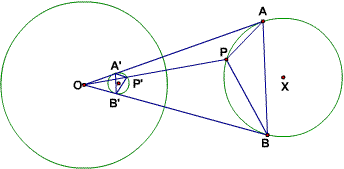
\includegraphics[scale=0.8]{invertcir2}    
\end{center}
%------------------
%-- Message Achilleas ( moderator )
Let circle X be our original circle.  We wish to show that the image of X when inverted about circle O is the little circle shown.  We start with the points of tangency when tangents to circle X from point O are drawn.  These are points A and B.  Let A' and B' be the images of these points.  Hence,

%------------------
%-- Message Achilleas ( moderator )
$$  OA \cdot OA' = OB \cdot OB' = r^2, $$
where r is the radius of circle O.

%------------------
%-- Message Achilleas ( moderator )
We wish to show that the image of point P is on the little circle.

%------------------
%-- Message Achilleas ( moderator )
Let P' be the image of P (so $OP \cdot OP' = r^2$ also).  Given any point P on that arc AB and its image P', what will we have to prove to determine that P' is on that little circle?

%------------------
%-- Message Achilleas ( moderator )
Any ideas?

%------------------
%-- Message MathJams ( user )
% We need to angle chase

%------------------
%-- Message Achilleas ( moderator )
We wish to show that angle $A'P'B'$ is constant (it is $A'B'O$ in particular).  How can we do so?

%------------------
%-- Message Achilleas ( moderator )
We've used similar triangles all over the place today; can we use them here?

%------------------
%-- Message Achilleas ( moderator )
We know that $OA \cdot OA' = OP \cdot OP'$, so $\dfrac{OA}{OP} = \dfrac{OP'}{OA'}$.  Since $\angle A'OP' = \angle POA$, we have $\triangle OAP \sim OP'A'$.  How does this help?  (Remember, we want to prove something about $\angle A'P'B'$.)

%------------------
%-- Message coolbluealan ( user )
% $\angle OP'A'=\angle OAP$

%------------------
%-- Message Achilleas ( moderator )
Focusing on the angle we care about (or part of it), we see that $\angle A'P'O = \angle PAO$ from our triangle similarity.  Hence, $\angle A'P'O = (\text{arc }AP)/2$.

%------------------
%-- Message Achilleas ( moderator )
Now what?

%------------------
%-- Message MathJams ( user )
% $\angle OP'B'=\angle OBP$

%------------------
%-- Message Achilleas ( moderator )
We can do the same for $B'P'O$: $\triangle B'P'O \sim \triangle PBO$, so $\angle B'P'O = \angle PBO = (\text{arc } PB)/2$.  So?

%------------------
%-- Message pritiks ( user )
% angle A'P'B' is constant

%------------------
%-- Message Achilleas ( moderator )
% Why?

%------------------
%-- Message coolbluealan ( user )
% $\angle A'P'B'=(arc AP)/2+(arc BP)/2=(arc AB)/2$

%------------------
%-- Message MathJams ( user )
% Show $\angle A'P'B' = \angle A'OP'+\angle OP'B'=\angle APB$

%------------------
%-- Message dxs2016 ( user )
% angle A'P'B = angle OAP + angle OBP = (arc AB) /2

%------------------
%-- Message Achilleas ( moderator )
$\angle A'P'B' = \angle A'P'O + \angle B'P'O = (\text{arc }AP + \text{arc }PB)/2 = (\text{arc }AB)/2$, which is a constant  Hence, $P'$ is on an arc of a circle through $A'$ and $B'$.

%------------------
%-- Message Achilleas ( moderator )
What else would we have to do to finish the proof?

%------------------
%-- Message Lucky0123 ( user )
% Show that all points on the circle are acquirable

%------------------
%-- Message Achilleas ( moderator )
We'd have to take care of the case in which $P$ is on the major arc $AB$, showing that it leads to a $P'$ such that $A'P'B'$ is the supplement of the $A'P'B'$ found above (thus it is on the same circle, just on the other `side' of $A'B'$ ).  We'd also have to show that every $P'$ is in the image upon inversion of circle $X$.

%------------------
%-- Message Achilleas ( moderator )
The details of that proof are essentially the same as the proof we just did.

%------------------
%-- Message Achilleas ( moderator )
Hence, the inverse of a circle that does not pass through the center of the circle we're inverting about is another circle.

%------------------
%-- Message Achilleas ( moderator )
\bigskip
\centerline{\rule{13cm}{0.4pt}}
Here's a quick summary of what happens to some things we've found.

%------------------
%-- Message Achilleas ( moderator )
1. Lines through the center of inversion go to themselves.

%------------------
%-- Message Achilleas ( moderator )
2. Lines not through the center of inversion go to circles that pass through the center of inversion.

%------------------
%-- Message Achilleas ( moderator )
3. Circles through the center of inversion go to lines (that don't pass through the center of inversion).

%------------------
%-- Message Achilleas ( moderator )
4. Circles not through the center of inversion go to circles not through the center of inversion.

\centerline{\rule{13cm}{0.4pt}}
\bigskip
%------------------
%-- Message Achilleas ( moderator )
In the so-called inversive plane (the plane with our point at infinity added), it's often convenient to think of lines as circles that pass through the point at infinity.

%------------------
%-- Message Achilleas ( moderator )
Using this abuse of notation, all these results can be summarized as follows: inversion takes circles to circles.

%------------------
%-- Message Achilleas ( moderator )
Whether they're bona-fide circles or actually lines that we're pretending are circles depends on whether the ``circle" in question passes through the point at infinity.

%------------------
%-- Message Achilleas ( moderator )
By the way, usually lines intersect at only one point. But circles typically intersect at two points, if they intersect at all.

%------------------
%-- Message Achilleas ( moderator )
So in our inversion scheme where lines are actually circles, shouldn't there typically be two intersection points? What's going on?

%------------------
%-- Message Achilleas ( moderator )
Where is the missing intersection point?

%------------------
%-- Message MeepMurp5 ( user )
% the point at infinity

%------------------
%-- Message JacobGallager1 ( user )
% One of those points is the point at infinity

%------------------
%-- Message SlurpBurp ( user )
% the other point is $P_\infty$?

%------------------
%-- Message Ezraft ( user )
% at infinity

%------------------
%-- Message Achilleas ( moderator )
Right! Every pair of lines is considered to intersect at the point at infinity.

%------------------
%-- Message Achilleas ( moderator )
We even say that parallel lines are tangent at the point at infinity!

%------------------
%-- Message Achilleas ( moderator )
So in inversive geometry land, every pair of lines intersects. (In fact, lines always intersect twice, but maybe twice at the same point---like a polynomial having a repeated root.)

%------------------
%-- Message Achilleas ( moderator )
In a certain sense, it's 1-dimensional complex projective geometry.

%------------------
%-- Message Achilleas ( moderator )
\bigskip
Now we'll talk about what is \textbf{preserved} when we take inversions.

%------------------
%-- Message Achilleas ( moderator )
Is length preserved (i.e. if $A'$ and $B'$ are the inverse of $A$ and $B$, is $A'B' = AB$)?

%------------------
%-- Message MathJams ( user )
% No

%------------------
%-- Message SlurpBurp ( user )
% no

%------------------
%-- Message coolbluealan ( user )
% No

%------------------
%-- Message ca981 ( user )
% NO

%------------------
%-- Message smileapple ( user )
% no?

%------------------
%-- Message JacobGallager1 ( user )
% No

%------------------
%-- Message mustwin_az ( user )
% No

%------------------
%-- Message Trollyjones ( user )
% no

%------------------
%-- Message leoouyang ( user )
% No?

%------------------
%-- Message Gamingfreddy ( user )
% no

%------------------
%-- Message Ezraft ( user )
% no

%------------------
%-- Message Achilleas ( moderator )
No, length is not preserved in general.  Take $A$ to be on the circle and $B$ to be very close to the center - then $A'B'$ can be arbitrarily long.  (Or put $A$ and $B$ both very close to the center such that the center is on segment $AB$ - their images will be very far apart.)

%------------------
%-- Message Achilleas ( moderator )
How about \textbf{angles}?  What do we need to define to talk about angles?

%------------------
%-- Message Ezraft ( user )
% angles made by the intersection of two circles

%------------------
%-- Message Achilleas ( moderator )
First we need a way to talk about angles formed by intersecting circles.  What is a good way to assign an angle measure to how two intersecting circles meet?

%------------------
%-- Message coolbluealan ( user )
% angle formed by the tangents at the intersection point

%------------------
%-- Message Achilleas ( moderator )
We call the angle between the tangents at the intersection point of the circles the angle between the two circles.  (Generally, we'll use the acute angle, assuming the tangents aren't perpendicular.)

%------------------
%-- Message Achilleas ( moderator )
% https://s3.amazonaws.com/classroom.artofproblemsolving.com/Classes/GeomOlympiad/Images/intcir.gif
\begin{center}
    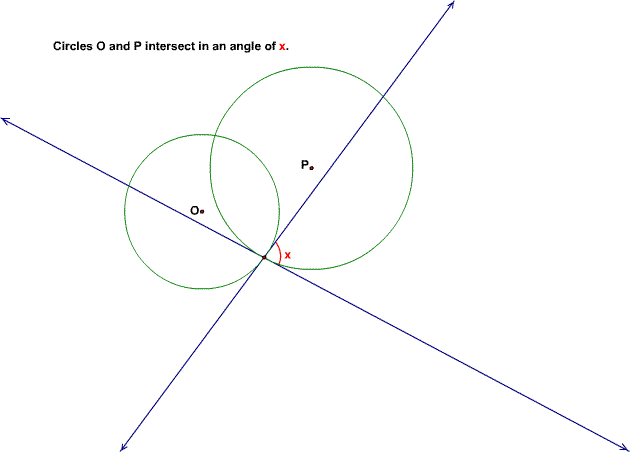
\includegraphics[scale=0.5]{intcir}    
\end{center}
%------------------
%-- Message Achilleas ( moderator )
If the tangents are perpendicular, we call the circles \textbf{orthogonal}.  Circles which are tangent intersect in a 0 degree angle.

%------------------
%-- Message Achilleas ( moderator )
Now that we have a definition for the angle between two circles, we can investigate whether angles are preserved.  Consider first an inversion about a circle centered at the intersection point of the two circles.  What happens?  (I've left in the tangent lines so we can talk about angles.)

%------------------
%-- Message Achilleas ( moderator )
% https://s3.amazonaws.com/classroom.artofproblemsolving.com/Classes/GeomOlympiad/Images/interinv.gif
\begin{center}
    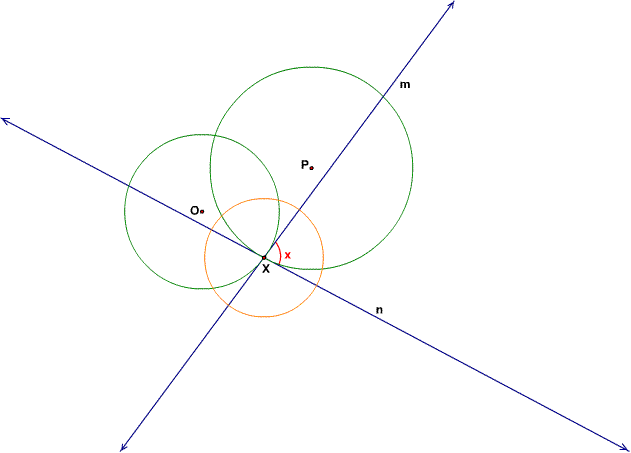
\includegraphics[scale=0.5]{interinv}    
\end{center}
%------------------
%-- Message Achilleas ( moderator )
Suppose we invert about the orange circle X in the diagram, which has a center at X, one of the points of intersection of our green circles.  What is the image of circle P?

%------------------
%-- Message dxs2016 ( user )
% line

%------------------
%-- Message Riya_Tapas ( user )
% a line

%------------------
%-- Message Ezraft ( user )
% a line

%------------------
%-- Message mustwin_az ( user )
% A line

%------------------
%-- Message Achilleas ( moderator )
The image of circle P is a line since P goes through the center of our circle of inversion (point X).  Specifically what line?

%------------------
%-- Message JacobGallager1 ( user )
% It is the radical axis of the orange circle and circle P

%------------------
%-- Message Gamingfreddy ( user )
% the line through the intersections of circle P and the orange circle

%------------------
%-- Message coolbluealan ( user )
% radical axis of circle P and circle X

%------------------
%-- Message Achilleas ( moderator )
The points where circle P and circle X intersect must be in the image, so the line goes through those points.

%------------------
%-- Message Achilleas ( moderator )
Similarly, the image of O is a line through the points of intersection of O and X:

%------------------
%-- Message Achilleas ( moderator )
% https://s3.amazonaws.com/classroom.artofproblemsolving.com/Classes/GeomOlympiad/Images/consangl.gif
\begin{center}
    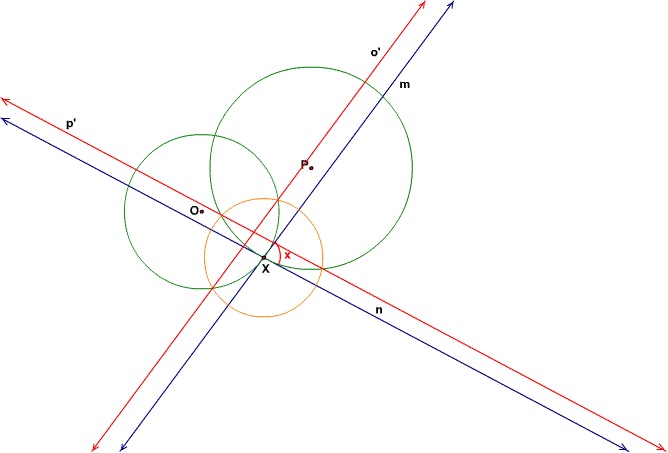
\includegraphics[scale=0.5]{consangl}    
\end{center}
%------------------
%-- Message Achilleas ( moderator )
Line $p'$ is the image of circle $P$ and line $o'$ is the image of circle $O$.  See anything interesting?

%------------------
%-- Message coolbluealan ( user )
% parallel lines

%------------------
%-- Message pritiks ( user )
% the lines are parallel

%------------------
%-- Message Achilleas ( moderator )
% Which lines are parallel?

%------------------
%-- Message Lucky0123 ( user )
% m is parallel to o' and n is parallel to p'

%------------------
%-- Message bryanguo ( user )
% $p' \parallel n$ and $o' \parallel m$

%------------------
%-- Message MathJams ( user )
% o'//m and p'//n

%------------------
%-- Message pritiks ( user )
% p' || n and o'|| m

%------------------
%-- Message Achilleas ( moderator )
It looks like $p' \parallel n$ and $o' \parallel m$.  Is it true?

%------------------
%-- Message Lucky0123 ( user )
% Yes

%------------------
%-- Message mustwin_az ( user )
% yes

%------------------
%-- Message coolbluealan ( user )
% yes

%------------------
%-- Message bryanguo ( user )
% yes

%------------------
%-- Message RP3.1415 ( user )
% yes

%------------------
%-- Message Gamingfreddy ( user )
% Yes

%------------------
%-- Message Achilleas ( moderator )
Since $n$ is tangent to circle $P$, we know that $n$ is perpendicular to $XP$.  We also know that $p'$ is perpendicular to $XP$ since it is a common chord.  Hence $n \parallel p'$.  Similarly, $o' \parallel m$.  So what do we conclude?

%------------------
%-- Message coolbluealan ( user )
% inversion centered on an intersection point between 2 circles preserves angles

%------------------
%-- Message AOPS81619 ( user )
% Inversion preserves the angle between two circles

%------------------
%-- Message Achilleas ( moderator )
We conclude that the images of circles $O$ and $P$ (which are lines $o'$ and $p'$ ) intersect in the same angle as the circles $O$ and $P$ (this is the angle between $m$ and $n$).

%------------------
%-- Message Achilleas ( moderator )
So, what if we invert any two lines about any point?  Will the angle between their image circles equal the angle between the lines?

%------------------
%-- Message MathJams ( user )
% yes

%------------------
%-- Message Lucky0123 ( user )
% yes.

%------------------
%-- Message bryanguo ( user )
% yes $ $

%------------------
%-- Message Achilleas ( moderator )
Yes - we just take the proof we just did and run it backwards.

%------------------
%-- Message Achilleas ( moderator )
We can extend this argument to show that angles are preserved under inversion.

%------------------
%-- Message Achilleas ( moderator )
(Here I will write primes for the images of everything under an inversion.)  For two circles $O$ and $P$ intersecting at point $X$ at an angle theta, draw the tangents $Q$ and $R$ at the point of intersection.  Inverting about any point you like, circles $Q'$ and $R'$ intersect at angle theta.  $O'$ and $P'$ must be tangent to $Q'$ and $R'$ respectively at $X'$, therefore the angle between $O'$ and $P'$ is theta.

%------------------
%-- Message Achilleas ( moderator )
Two important results of this are the following:

%------------------
%-- Message Achilleas ( moderator )
1) What happens if we invert two tangent circles?

%------------------
%-- Message MTHJJS ( user )
% parallel lines

%------------------
%-- Message Achilleas ( moderator )
% Or..

%------------------
%-- Message mustwin_az ( user )
% still tangent circles

%------------------
%-- Message ca981 ( user )
% or two tangent circles

%------------------
%-- Message Achilleas ( moderator )
% Or...

%------------------
%-- Message ca981 ( user )
% One circle and a tangent

%------------------
%-- Message MTHJJS ( user )
% tangent line to circle

%------------------
%-- Message Achilleas ( moderator )
The images of two tangent circles will always be two tangent circles, or a line tangent to a circle, or a pair of parallel lines, since the images must have an angle of 0.  (If you think of lines as circles with infinite radius, you don't even have to think of the line case as a separate case.)

%------------------
%-- Message Achilleas ( moderator )
Similarly, if you have a line tangent to a circle, any inversion will result in two tangent circles (or a line tangent to a circle).

%------------------
%-- Message Achilleas ( moderator )
This is one reason we think of inversion in problems with lots of tangency.

%------------------
%-- Message Achilleas ( moderator )
2) Suppose circles O and P are orthogonal - what happens if we invert circle O about circle P?

%------------------
%-- Message Achilleas ( moderator )
% https://s3.amazonaws.com/classroom.artofproblemsolving.com/Classes/GeomOlympiad/Images/orthocir.gif
\begin{center}
    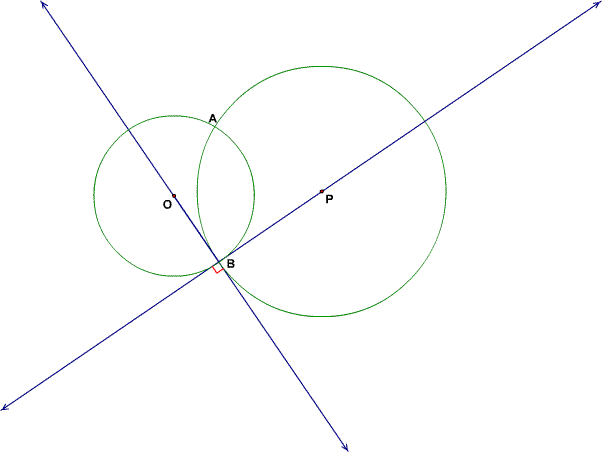
\includegraphics[scale=0.5]{orthocir}    
\end{center}

%------------------
%-- Message Achilleas ( moderator )
First, what shape do we expect to get?

%------------------
%-- Message Lucky0123 ( user )
% A circle

%------------------
%-- Message MathJams ( user )
% A circle

%------------------
%-- Message Wangminqi1 ( user )
% a circle

%------------------
%-- Message Riya_Tapas ( user )
% A circle

%------------------
%-- Message bryanguo ( user )
% a circle

%------------------
%-- Message Achilleas ( moderator )
We know the image of $O$ is a circle.

%------------------
%-- Message Achilleas ( moderator )
Do we know any points that this circle passes through?

%------------------
%-- Message coolbluealan ( user )
% A and B

%------------------
%-- Message MTHJJS ( user )
% A,B

%------------------
%-- Message Wangminqi1 ( user )
% $A$ and $B$

%------------------
%-- Message ca981 ( user )
% A and B

%------------------
%-- Message JacobGallager1 ( user )
% $A$ and $B$

%------------------
%-- Message dxs2016 ( user )
% A and B

%------------------
%-- Message bryanguo ( user )
% points A and B

%------------------
%-- Message mark888 ( user )
% $A$ and $B$

%------------------
%-- Message J4wbr34k3r ( user )
% A and B.

%------------------
%-- Message Riya_Tapas ( user )
% Points A and B

%------------------
%-- Message SlurpBurp ( user )
% $A$, $B$

%------------------
%-- Message Achilleas ( moderator )
We know it goes through A and B since A and B are on circle P.

%------------------
%-- Message Achilleas ( moderator )
Can you see which circle it is?

%------------------
%-- Message Achilleas ( moderator )
(Hint: We have not used orthogonality yet.)

%------------------
%-- Message MathJams ( user )
% circle O inverts to itself

%------------------
%-- Message JacobGallager1 ( user )
% So, the circle $O$ is preserved by inversion

%------------------
%-- Message MTHJJS ( user )
% circle O

%------------------
%-- Message AOPS81619 ( user )
% Is it the same as circle $O$?

%------------------
%-- Message Achilleas ( moderator )
We know that the image of circle O is perpendicular to P, so the radii of the image to points A and B are perpendicular to PA and PB.  Hence, the image of circle O is circle O.

%------------------
%-- Message Achilleas ( moderator )
Alternatively,  since the lines PA and PB are tangent to circle O, and they are fixed by the inversion, it follows that they will also be tangent to the image of circle O. Hence, the image of circle O is circle O.

%------------------
%-- Message Achilleas ( moderator )
Thus, a circle that is \textbf{orthogonal} to the circle we are inverting about is \textbf{fixed} under the inversion.

%------------------
%-- Message Achilleas ( moderator )
% Phewww...

%------------------
%-- Message Achilleas ( moderator )
\subsection{USING INVERSION ON OLYMPIAD PROBLEMS}

%------------------
%-- Message Riya_Tapas ( user )
% Problem time!

%------------------
%-- Message Achilleas ( moderator )
Now (finally) we are ready for some regular problems.

%------------------
%-- Message Achilleas ( moderator )
A couple general remarks on using inversion.  First, when you invert, you usually don't need to specify what circle you are inverting about, only its center.  Using a different circle will just result in a scaled diagram, which shouldn't make any difference.

%------------------
%-- Message Achilleas ( moderator )
Also, our last few facts give us some clues as to problems in which inversion might be useful.  Almost always, the problem must involve circles.  Usually, these circles will be tangent or orthogonal.  Also, there may be lines tangent to the circles.  And if you have a lot of lines and/or circles passing through the same point, that point is a good candidate for the center of inversion.

%------------------
%-- Message Achilleas ( moderator )
Inversion, as I noted at the beginning, seems a little magical, at least at first.  In general, you shouldn't ever spend a great deal of time trying it - usually it blows apart problems pretty quickly if it will work at all.  If you see a problem that feels like an inversion problem (probably because you've solved similar problems with inversion), try it briefly, but don't get too tied to it.

%------------------
%-- Message Achilleas ( moderator )
\begin{example}
Given a circle and two fixed points $A$ and $B$ on the circle, consider all possible of pairs of circles tangent to the given circle at $A$ and $B$ and to each other.  Find the locus of the point where the two new circles are tangent.    
\end{example}

%------------------
%-- Message Achilleas ( moderator )
% https://s3.amazonaws.com/classroom.artofproblemsolving.com/Classes/GeomOlympiad/Images/3tancirc.gif
\begin{center}
    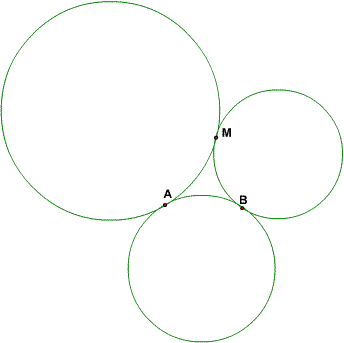
\includegraphics[scale=0.5]{3tancirc}    
\end{center}
%------------------
%-- Message Achilleas ( moderator )
What makes us think of inversion?

%------------------
%-- Message SlurpBurp ( user )
% tangent circles

%------------------
%-- Message smileapple ( user )
% circles and tangency

%------------------
%-- Message MathJams ( user )
% A ton of circles and tangencys

%------------------
%-- Message pritiks ( user )
% tangent circles

%------------------
%-- Message JacobGallager1 ( user )
% All the tangent circles

%------------------
%-- Message coolbluealan ( user )
% tangent circles

%------------------
%-- Message mark888 ( user )
% circles and tangents

%------------------
%-- Message Achilleas ( moderator )
We have circles galore, and they're all tangent.  We think of inversion because we know that we can invert tangent circles into parallel lines, which are easier to deal with than circles.

%------------------
%-- Message Achilleas ( moderator )
How can we invert tangent circles into parallel lines?

%------------------
%-- Message Achilleas ( moderator )
(we invert about a circle, not a point)

%------------------
%-- Message Riya_Tapas ( user )
% What are we inverting with respect to? Which circle

%------------------
%-- Message Achilleas ( moderator )
% This was my question. https://artofproblemsolving.com/assets/images/smilies/classroom-smile.gif

%------------------
%-- Message AOPS81619 ( user )
% A circle centered at the point of tangency

%------------------
%-- Message MathJams ( user )
% Invert about a circle with it's center as the tangency point

%------------------
%-- Message Achilleas ( moderator )
If we invert two tangent circles about a circle centered at the point of tangency, the image of the two circles will be two parallel lines (since the images are distinct lines and they can only intersect at the 'point at infinity'.

%------------------
%-- Message Achilleas ( moderator )
What should we choose as our center?  Should we choose point M (the point of tangency of the two new circles)?

%------------------
%-- Message MathJams ( user )
% We should choose A or B

%------------------
%-- Message coolbluealan ( user )
% A or B

%------------------
%-- Message Achilleas ( moderator )
Why not $M$?

%------------------
%-- Message JacobGallager1 ( user )
% We're trying to find the locus of $M$, so perhaps not? Our center of inversion should be a static point like A or B

%------------------
%-- Message coolbluealan ( user )
% we don't know where it is yet

%------------------
%-- Message MathJams ( user )
% Since we do not know where M is

%------------------
%-- Message smileapple ( user )
% $A$ and $B$ are fixed, whereas $M$ isn't

%------------------
%-- Message ca981 ( user )
% Not able to find locus of M

%------------------
%-- Message dxs2016 ( user )
% we're trying to find locus

%------------------
%-- Message Achilleas ( moderator )
We're not too happy with choosing M as the center of inversion, since that varies.  We're far more interested in seeing what happens to M under some other inversion, since then we might be able to say something about how M varies before inversion.

%------------------
%-- Message Achilleas ( moderator )
All that's left is inverting with respect to a circle centered at A or at B.  Let's choose A (doesn't matter which we choose).

%------------------
%-- Message Achilleas ( moderator )
If we invert about a circle centered at A with radius r, what will become of the two circles tangent at A?

%------------------
%-- Message Lucky0123 ( user )
% They become 2 parallel lines

%------------------
%-- Message JacobGallager1 ( user )
% They become parallel lines

%------------------
%-- Message ca981 ( user )
% Two parallel lines

%------------------
%-- Message Ezraft ( user )
% they will map to parallel lines

%------------------
%-- Message coolbluealan ( user )
% two parallel lines

%------------------
%-- Message MathJams ( user )
% two parallel lines

%------------------
%-- Message Achilleas ( moderator )
Circles passing through the center of inversion map to lines.  The images of circles tangent at the center of inversion are parallel lines, since the images can only intersect at the `point of infinity' (which is the image of their original intersection, the center of inversion).

%------------------
%-- Message Achilleas ( moderator )
Let's call these lines $m$ and $b$, with the image of $M$ (which we call $M'$ ) on $m$ and the image of $B (B' )$ on $b$.

%------------------
%-- Message Achilleas ( moderator )
That's pretty easy, all we have to worry about is the other circle.  What will its image be?

%------------------
%-- Message ca981 ( user )
% another circle

%------------------
%-- Message mustwin_az ( user )
% it will be a circle

%------------------
%-- Message coolbluealan ( user )
% a circle

%------------------
%-- Message MathJams ( user )
% Another circle

%------------------
%-- Message Achilleas ( moderator )
The image of a circle not passing through the center of inversion is another circle.

%------------------
%-- Message Achilleas ( moderator )
Do we know anything interesting about this image circle?

%------------------
%-- Message MTHJJS ( user )
% circle tangent to m, b

%------------------
%-- Message JacobGallager1 ( user )
% It will be a circle tangent to the two lines

%------------------
%-- Message Achilleas ( moderator )
The original circle through $B$ and $M$ was tangent to our original circles passing through $A$, so its image must be tangent to the images of those circles through $A$.  Hence, its image is tangent to both of our parallel lines $m$ and $b$.

%------------------
%-- Message Achilleas ( moderator )
How does this help?

%------------------
%-- Message JacobGallager1 ( user )
% This tells us that $M'B'$ is a diameter of the new circle

%------------------
%-- Message ca981 ( user )
% The circle is defined with diameter = distance between 2 parallel lines, and Passing M' and B'

%------------------
%-- Message Achilleas ( moderator )
We know that the image of $B$ is one of the tangency points of the image circle with the parallel lines.  Hence, if $B'$ is this image, we know our circle is tangent to $b$ at $B'$.  What does this tell us about $M'$?

%------------------
%-- Message Achilleas ( moderator )
$M'$ is the point on $m$ such that $B'M'$ is perpendicular to both $b$ and $m$:

%------------------
%-- Message Achilleas ( moderator )
% https://s3.amazonaws.com/classroom.artofproblemsolving.com/Classes/GeomOlympiad/Images/3taninv.gif
\begin{center}
    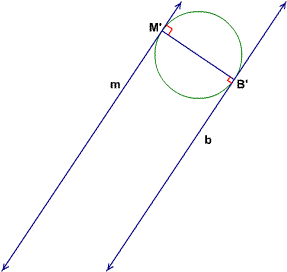
\includegraphics[scale=0.5]{3taninv}    
\end{center}

%------------------
%-- Message Achilleas ( moderator )
(Remember that $m$ and $M'$ here move while $b$ and $B'$ are fixed.)

%------------------
%-- Message Achilleas ( moderator )
How does this solve the problem?

%------------------
%-- Message Achilleas ( moderator )
Suppose for every possible pair of circles we perform this inversion with the same center and the same radius.  Line $b$ and point $B'$ are fixed - the inversion will always produce them exactly the same.  Point $M'$ will always appear on the other line such that $B'M'$ is perpendicular to line $b$.  Hence the locus of $M'$ is a line through $B'$ perpendicular to $b$.  Prove on your own why every point on this line is in the locus (other than $B'$ and the point at infinity).

%------------------
%-- Message Achilleas ( moderator )
Thus, what is the locus of $M$?

%------------------
%-- Message coolbluealan ( user )
% a circle

%------------------
%-- Message Achilleas ( moderator )
% How about a point on it?

%------------------
%-- Message Ezraft ( user )
% a circle that passes through $A$

%------------------
%-- Message ca981 ( user )
% B

%------------------
%-- Message coolbluealan ( user )
% B

%------------------
%-- Message MTHJJS ( user )
% A,B

%------------------
%-- Message Achilleas ( moderator )
We have found that the locus of the image of $M$ is a straight line not passing through the center of inversion.  Hence, the locus of $M$ is the inverse of the line's image.  The inverse of this line must be a circle through the center of inversion.

%------------------
%-- Message Achilleas ( moderator )
So that circle goes through $A$ and $B$.  Is there anything else we can say about it?

%------------------
%-- Message Achilleas ( moderator )
How is the new circle related to the original one?

%------------------
%-- Message coolbluealan ( user )
% orthogonal

%------------------
%-- Message ca981 ( user )
% orthogonal ?

%------------------
%-- Message MathJams ( user )
% orthogonal to our original circle

%------------------
%-- Message Achilleas ( moderator )
It is the circle through $A$ and $B$ that is orthogonal to the original circle.  We know this because the image of the locus of $M$ is orthogonal to $b$, so the locus of $M$ must be orthogonal to the inverse of $b$ (which is the original circle).

%------------------
%-- Message Achilleas ( moderator )
(Note that we have to exclude $A$ and $B$ themselves from the locus of $M$.)

%------------------
%-- Message Achilleas ( moderator )
Note also that the radius of inversion doesn't matter, so long as it's constant.

%------------------
%-- Message Achilleas ( moderator )
Last problem:

%------------------
%-- Message Achilleas ( moderator )
\begin{example}
Given two tangent circles and a point $P$ on their radical axis, construct with compass and ruler all the circles that are tangent to our original two circles and pass through the point $P$.
    
\end{example}

%------------------
%-- Message Achilleas ( moderator )
Why do we think of inversion?

%------------------
%-- Message Lucky0123 ( user )
% It has tangent circles

%------------------
%-- Message AOPS81619 ( user )
% tangency and circles

%------------------
%-- Message MathJams ( user )
% Tangency and circles and radical axis!

%------------------
%-- Message mark888 ( user )
% two tangent circles

%------------------
%-- Message Riya_Tapas ( user )
% Tangent circles

%------------------
%-- Message dxs2016 ( user )
% tangent circles

%------------------
%-- Message bryanguo ( user )
% because of the two tangent circles

%------------------
%-- Message Catherineyaya ( user )
% tangent and circles

%------------------
%-- Message Achilleas ( moderator )
We have tangent circles.  Also, point P is on the common tangent through the point of tangency of our two circles.

%------------------
%-- Message Achilleas ( moderator )
Thus we have 3 tangent figures, two circles and a line.  It's definitely worth thinking about inversion, even though it's a construction problem.

%------------------
%-- Message Achilleas ( moderator )
Here's what we're given:

%------------------
%-- Message Achilleas ( moderator )
% https://s3.amazonaws.com/classroom.artofproblemsolving.com/Classes/GeomOlympiad/Images/constinv.gif
\begin{center}
    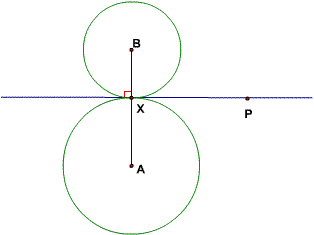
\includegraphics[scale=0.5]{constinv}    
\end{center}

%------------------
%-- Message Achilleas ( moderator )
We want the circles through P which are tangent to our other two circles.

%------------------
%-- Message Achilleas ( moderator )
It's not so obvious how to construct these circles.  Is it obvious how to construct any circles (or anything else, for that matter) which are tangent to both circles?

%------------------
%-- Message pritiks ( user )
% extend AB and draw a circle through the points it intersects with the circle

%------------------
%-- Message Achilleas ( moderator )
If we extend $AB$ to meet the circles again at $C$ and $D$, it's easy to construct the circle with diameter $CD$ - this one is tangent to both circles.

%------------------
%-- Message Achilleas ( moderator )
We also know how to construct the lines which are tangent to both circles.

%------------------
%-- Message Achilleas ( moderator )
Does either of these help us in our hunt for a circle through P which is tangent to the two circles?

%------------------
%-- Message Achilleas ( moderator )
Keeping in mind that we think inversion might be useful, can we find any way to relate any of our lines or circles we can construct to the circles we want?

%------------------
%-- Message Achilleas ( moderator )
What do we know about the images of two tangent objects under inversion?

%------------------
%-- Message Lucky0123 ( user )
% They are still tangent

%------------------
%-- Message JacobGallager1 ( user )
% They remain tangent

%------------------
%-- Message Achilleas ( moderator )
We know that the images of two tangent objects under inversion are themselves tangent.  How does this help?

%------------------
%-- Message Achilleas ( moderator )
We know that if we perform an inversion, it will map any circle or line that is tangent to both of our circles to something that is tangent to the images of our original circles.

%------------------
%-- Message Achilleas ( moderator )
So, do we just invert one of our tangent lines about P and voila - we have a circle tangent to our original circles?

%------------------
%-- Message MathJams ( user )
% No

%------------------
%-- Message Achilleas ( moderator )
Why not?

%------------------
%-- Message coolbluealan ( user )
% a circle tangent to the images of our original circles

%------------------
%-- Message Achilleas ( moderator )
The image of the tangent line will be tangent to the *images* of our circles.

%------------------
%-- Message Achilleas ( moderator )
But this does suggest another approach: what?

%------------------
%-- Message coolbluealan ( user )
% draw a tangent to the images of our original circle and then invert back

%------------------
%-- Message JacobGallager1 ( user )
% Take the image of the two circles under an inversion with center $P$. Draw common tangents from these images passing through the point $P$. Take the same inversion again, and you will have your desired circles

%------------------
%-- Message Achilleas ( moderator )
Invert both circles, find the two tangent lines to the *inverses*, and then invert back to get the circles we want.

%------------------
%-- Message Achilleas ( moderator )
That's a fine approach, and solves the problem.  To be a little more elegant though, we're actually going to choose a particular circle to invert around (centered at P) which leaves the original circles fixed and thus requires less work.

%------------------
%-- Message Achilleas ( moderator )
We need an inversion that leaves our circles unchanged.  What inversions leave circles unchanged?

%------------------
%-- Message Ezraft ( user )
% find an inversion such that circles $A$ and $B$ are the images

%------------------
%-- Message Achilleas ( moderator )
% How can we do that?

%------------------
%-- Message JacobGallager1 ( user )
% Orthogonal circles

%------------------
%-- Message MathJams ( user )
% Find a circle orthogonal to both circles

%------------------
%-- Message coolbluealan ( user )
% orthogonal circles

%------------------
%-- Message Achilleas ( moderator )
If two circles are orthogonal, then the image of each circle upon inverting about the other is itself.

%------------------
%-- Message JacobGallager1 ( user )
% Inverting about the circle centered at $P$ with radius $PX$ will leave the two circles fixed

%------------------
%-- Message Achilleas ( moderator )
Our inversion circle must be orthogonal to both circles since it must leave them unchanged.  Hence, we'll use a circle of inversion centered at $P$ with radius $PX$.

%------------------
%-- Message Achilleas ( moderator )
So, starting from just

%------------------
%-- Message Achilleas ( moderator )
% https://s3.amazonaws.com/classroom.artofproblemsolving.com/Classes/GeomOlympiad/Images/constinv.gif
\begin{center}
    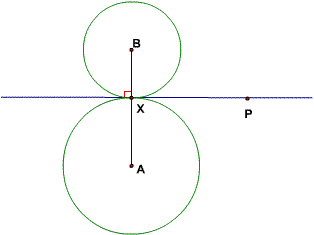
\includegraphics[scale=0.5]{constinv}    
\end{center}

%------------------
%-- Message Achilleas ( moderator )
How do we complete our construction?

%------------------
%-- Message coolbluealan ( user )
% construct a tangents to circle A and B, invert them with center P and radius PX

%------------------
%-- Message ca981 ( user )
% Draw common tangents of circle A and B

%------------------
%-- Message Achilleas ( moderator )
We construct our external tangents, and the circle with center P and radius XP:

%------------------
%-- Message Achilleas ( moderator )
% https://s3.amazonaws.com/classroom.artofproblemsolving.com/Classes/GeomOlympiad/Images/constinvstep.gif
\begin{center}
    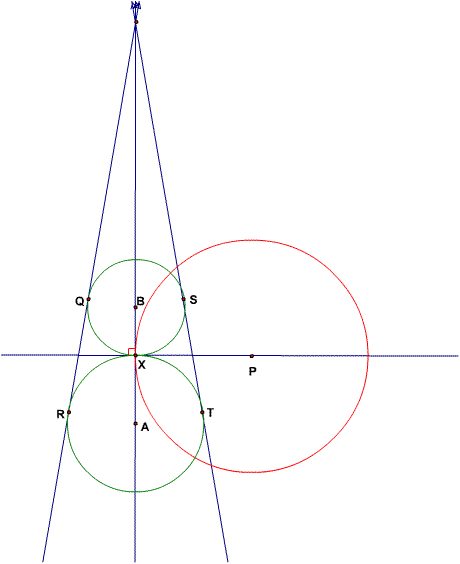
\includegraphics[scale=0.6]{constinvstep}    
\end{center}
%------------------
%-- Message Achilleas ( moderator )
How do we construct the inversions of the tangent lines?

%------------------
%-- Message MathJams ( user )
% Consider where points on these lines go

%------------------
%-- Message Achilleas ( moderator )
We know how to invert a point, so we can simply invert points to build our circle.  How many do we need to invert for each circle?

%------------------
%-- Message JacobGallager1 ( user )
% Just two, since we know they must also pass through $P$

%------------------
%-- Message MathJams ( user )
% 2 because it goes through P

%------------------
%-- Message Achilleas ( moderator )
We need only invert 2 points, as we know each image circle passes through P.  What points do we choose to invert and how can we construct their images quickly?

%------------------
%-- Message MathJams ( user )
% Invert the tangency points

%------------------
%-- Message mustwin_az ( user )
% invert S,T

%------------------
%-- Message Achilleas ( moderator )
We choose to invert Q and R to produce one circle, and S and T for the other.

%------------------
%-- Message Achilleas ( moderator )
How can we quickly find the image of R?

%------------------
%-- Message Achilleas ( moderator )
Do we know where it is on?

%------------------
%-- Message MathJams ( user )
% It is on circle A and  line PR

%------------------
%-- Message JacobGallager1 ( user )
% The second intersection of the line PR and the circle with center $A$

%------------------
%-- Message Achilleas ( moderator )
We know that the image of R must be on ray PR and that it must be on the lower circle (circle A), since the images of the inversions of QR and circle A must meet at the image of their intersection point (point R).

%------------------
%-- Message Achilleas ( moderator )
We can do the same to find the images of $Q, S,$ and $T$.  We call these images $R'$, $Q'$, $S'$, $T'$.  We then complete the problem by finding the circumcircles of $PR'Q'$ and $PS'T'$:

%------------------
%-- Message Achilleas ( moderator )
% https://s3.amazonaws.com/classroom.artofproblemsolving.com/Classes/GeomOlympiad/Images/constinv2cir.gif
\begin{center}
    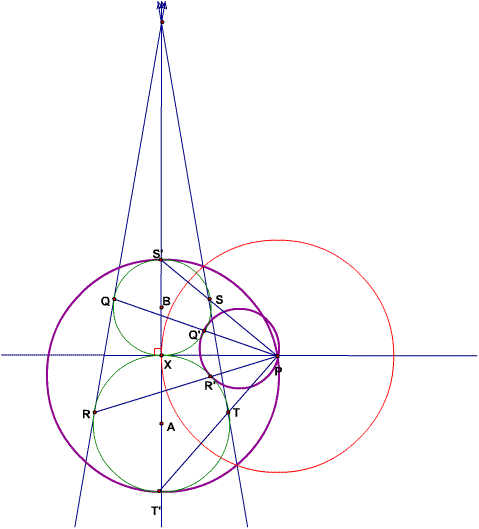
\includegraphics[scale=0.6]{constinv2cir}    
\end{center}

%------------------
%-- Message Achilleas ( moderator )
Both circles are shown in the figure.

%------------------
%-- Message Achilleas ( moderator )
Notice that we can use this approach to prove that there are at most 2 circles that fit the specifications of the problem (circle through P, tangent to the other two).

%------------------
%-- Message Achilleas ( moderator )
That's it for tonight.  With practice on the board and the final Challenge Set, you should get more used to using inversion in problems involving tangency.

%------------------
%-- Message Achilleas ( moderator )
Once again, don't spend forever with inversion on a problem. If it works, it usually works quickly.

%------------------
%-- Message Achilleas ( moderator )
If you don't get anywhere in 15 minutes, try something else (and I wouldn't reach for it first if something else, like homothety or good old angle chasing/power of a point looked good).

%------------------
%-- Message Achilleas ( moderator )
You could read about inversion in EGMO. I also like Stankova's exposition on inversion a lot!

%------------------
%-- Message Achilleas ( moderator )
See \url{https://mathcircle.berkeley.edu/sites/default/files/BMC6/ps0405/inversionSJ04.pdf}

%------------------
%-- Message Achilleas ( moderator )
There is another cool handout, by Dusan Dukic, one of the authors of the IMO compendium.

%------------------
%-- Message Achilleas ( moderator )
\url{https://memo.szolda.hu/feladatok/inversion_ddj.pdf}

%------------------
%-- Message Achilleas ( moderator )
You will see more Olympiad problems there!

%------------------
%-- Message MathJams ( user )
% what's after this class?

%------------------
%-- Message Achilleas ( moderator )
% Chaos.

%------------------
%-- Message pritiks ( user )
% lol

%------------------
%-- Message Ezraft ( user )
% https://artofproblemsolving.com/assets/images/smilies/classroom-boggle.gif

%------------------
%-- Message Achilleas ( moderator )
% https://artofproblemsolving.com/assets/images/smilies/classroom-smile.gif

%------------------
%-- Message Achilleas ( moderator )
There is no AoPS class after this one, other than WOOT.

%------------------
%-- Message Achilleas ( moderator )
There are many concepts/ideas/tools that we did not cover.

%------------------
%-- Message MathJams ( user )
% any recommended books?

%------------------
%-- Message Achilleas ( moderator )
One of my favorites is \emph{Solving Problems In Geometry: Insights And Strategies For Mathematical Olympiad And Competitions, by Kim Hoo Hang and Haibin Wang}.

What I like about it is that it gives insights about every solved example before presenting the neatly written solution to many math Olympiad problems. It includes ``a list of commonly used facts, useful skills, and problem-solving strategies and it will help you tackle challenging geometry problems at high-level Mathematics competitions."

You will learn a lot, but you won't find other useful stuff there, such as transformations, inversion, etc. But you will be well-equipped to move on to the students' favorite book in Olympiad geometry, which is EGMO by E.Chen.

%------------------
%-- Message Achilleas ( moderator )
Also, more importantly:

%------------------
%-- Message Achilleas ( moderator )
Solve problems...

%------------------
%-- Message Achilleas ( moderator )
Solve problems...

%------------------
%-- Message Achilleas ( moderator )
Solve problems...

%------------------
%-- Message Achilleas ( moderator )
And...study new stuff.

%------------------
%-- Message Achilleas ( moderator )
% I guess that's really it for today!

%------------------
%-- Message Achilleas ( moderator )
% Do not forget our survey. Thank you all! See you around! It was great teaching this class! 

%------------------
	
\section{Message Board}
\Writetofile{hints}{\protect\section{Message Board 12}}
\Writetofile{soln}{\protect\newpage\protect\section{Message Board 12}}

\subsection{Problem 1}
Given a circle and a line that does not intersect the circle, construct the inverse of the line with respect to the circle.

\begin{mdsoln}
In case we are not given the center $O$ of the given circle, we can construct it by picking three distinct points of the circle and finding the circumcenter of the triangle they form.

Let $P$ be the foot of the altitude from $O$ to the given line $\ell$. We know that $\ell$ maps to a circle $\omega$ through $O$. By symmetry, $\omega$ must have diameter $OP'$, where $P'$ is the inverse of $P$. We construct $P'$ as described in class, by drawing a tangent $PX$ to the given circle (where $X$ is on the given circle) and finding the foot of the altitude from $X$ to the segment $OP$.

Having located $P'$, it is simple to construct $\omega$ as the circle with diameter $OP'$.
    
\end{mdsoln}

\subsection{Problem 2}
Given a circle and a line that intersects the circle in two non-diametrically opposed points, prove that the inverse of the line with respect to the circle is a circle. Prove that if the line is tangent to the circle, the image of the line is still a circle. (We want the details of the proof that the inverses of the lines described are circles - don't just say 'the inverse of a line not through the center of inversion is a circle')

\begin{mdsoln}    
Let $\omega$ be the circle, with center $O$. Let $\ell$ be the line, and consider first the case where $\ell$ intersects $\omega$ in two distinct points $A$ and $B$.

Let $P$ be on $\ell$ (and distinct from $A$ and $B$). Let $P'$ be the inverse of $P$. Observe that since $(OP)(OP')=OA^2=OB^2$, we must have $\triangle OAP\sim \triangle OP'A$ and $\triangle OBP\sim \triangle OP'B$.

Consider first the case where $P$ is on segment $AB$. Then, $\angle P'AO+\angle OBP'=\angle OPA+\angle BPO=180^\circ$, so $P'$ lies on the circumcircle of $\triangle OAB$.

Now suppose $P$ is not on segment $AB$. Then, $\angle OAP'=\angle APO=\angle BPO=\angle OBP'$, so in this case also $P'$ must lie on the (fixed) circumcircle of $\triangle OAB$.

Clearly, $O$ is in the inverse of $\ell$ since the point at infinity (which is on $\ell$) maps to $O$. Now consider a point $Q$ on $\omega_1$ distinct from $O$. Ray $OQ$ must intersect $\ell$ at some point $Q'$. Then, our argument above shows that the inverse of $Q'$ must be a point on $OQ$ that is also on $\omega_1$ - this point, since it is clearly not $O$, must be $Q$, showing that all points on $\omega_1$ are the images of points on $\ell$ and completing the proof that $\omega_1$ is the image of $\ell$ under inversion about $\omega$.

Now suppose that $\ell$ is tangent to $\omega$ at some point $A$. Pick some point $P$ on $\ell$ with inverse $P'$. Since $(OP)(OP')=OA^2$, we must have $\triangle OAP\sim \triangle OP'A$. Hence, $\angle AP'O$ is a right angle, so $P'$ must be on the circle $\omega_2$ with diameter $OA$.

Conversely, if $Q$ is any point of $\omega_2$, we can use our previous argument to show that $Q$ is the image of a point on $\ell$. We conclude that $\ell$ maps to $\omega_2$.
\end{mdsoln}

\subsection{Problem 3}
Find a quick proof of Ptolemy’s Inequality using one of the facts about inversion we learned in class. (Reminder: Ptolemy’s Inequality states that if $A, B, C, D$ are points in a plane, then $AB \cdot CD + AD\cdot BC \geq AC\cdot BD$, with equality if and only if the four points are concyclic.)

\textit{Has hints.}
\begin{sketch}
    \begin{enumerate}
        \item Invert with respect to A with an arbitrary radius.
        \item Use the result of problem 2 on the final.
    \end{enumerate}
\end{sketch}

\begin{mdsoln}
Invert with respect to a circle centered at $A$ of arbitrary radius $r$, so that $B,C,D$ go to $B',C',D'$, respectively. Then, by the Triangle Inequality, $C'D'+B'C'\ge B'D'$. Equality occurs if and only if $B',C',D'$ are collinear in that order, which happens if and only if $ABCD$ is a convex cyclic quadrilateral (or $B,C,D$ lie in that order on a line passing through $A$, which might be seen as a limiting case of $ABCD$ cyclic with an infinitely large circumcircle).

Observe that $AB=r^2/AB'$, $AC=r^2/AC'$, and $AD=r^2/AD'$. Using the formula from 2b on the Final Challenge Set (relating distances after inversion to distances before), we find that since $BC$ is the image of $B'C'$ under an inversion about a circle of radius $r$ centered at $A$,$$BC=\frac{r^2(B'C')}{(AB')(AC')}$$and similar expressions for $B'D'$ and $C'D'$. Hence,\begin{eqnarray*}AB\cdot CD+AD\cdot BC&=&\frac{r^2}{AB'}\cdot \frac{r^2(C'D')}{(AC')(AD')}+\frac{r^2}{AD'}\cdot \frac{r^2(B'C')}{(AB')(AC')}\\ &=&\frac{r^4}{(AB')(AC')(AD')}(C'D'+B'C')\\ &\ge &\frac{r^4}{(AB')(AC')(AD')}(B'D')\\ &=&\frac{r^2}{AC'}\cdot \frac{r^2(B'D')}{(AB')(AD')}\\ &=&AC\cdot BD\end{eqnarray*}with equality if and only if $ABCD$ is cyclic.    
\end{mdsoln}

\subsection{Problem 4}
Circles $A$, $B$, and $C$ all pass through point $X$. The radical axis of circles $A$ and $B$ passes through the center of $C$; the radical axis of circles $B$ and $C$ passes through the center of $A$. Prove that the radical axis of $A$ and $C$ passes through the center of $B$.

% https://s3.amazonaws.com/classroom.artofproblemsolving.com/Classes/GeomOlympiad/Images/threerads.gif
\begin{center}
    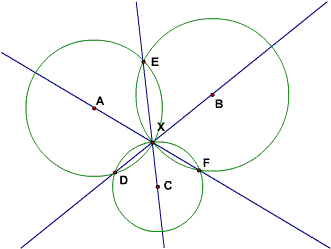
\includegraphics[scale=0.6]{threerads}
\end{center}

\begin{mdsoln}
Invert about a circle of arbitrary radius centered at the point $X$. Circles $A,B,C$ invert to lines $\ell_A,\ell_B,\ell_C$, respectively. Let $\ell_A$ and $\ell_B$ meet at $C_1$. Define $A_1$ and $B_1$ similarly. Let $m_A$ be the radical axis of circles $B$ and $C$. Define $m_B$ and $m_C$ similarly. Clearly, $m_A$, $m_B$, and $m_C$ invert to themselves, since they all pass through $X$. Then, note that $m_A$ must in fact be the line $A_1X$; likewise, $m_B$ and $m_C$ are $B_1X$ and $C_1X$ respectively. Since $m_C$ passes through the center of $C$, it is perpendicular to circle $C$ and so must be perpendicular to $\ell_C$. Then, $C_1X\perp A_1B_1$. Likewise, since $m_A$ passes through the center of $A$, $A_1X\perp B_1C_1$. Hence, $X$ must be the orthocenter of $\triangle A_1B_1C_1$. Therefore, $B_1X\perp A_1C_1$, implying that $m_B\perp \ell_B$. Therefore, $m_B$ must be perpendicular to circle $B$ and so must pass through its center, as desired.    
\end{mdsoln}

\subsection{Problem 5}
We are given four points $A$, $B$, $C$, and $D$ such that no 3 are collinear. Prove that the angle between the circles circumscribed about triangles $ABC$ and $BCD$ is equal to the angle between the circles circumscribed about the triangles $CDA$ and $DAB$.

% https://s3.amazonaws.com/classroom.artofproblemsolving.com/Classes/GeomOlympiad/Images/circangl.gif
\begin{center}
    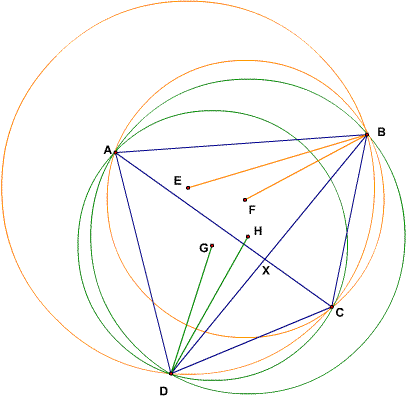
\includegraphics[scale=0.6]{circangl}
\end{center}
\begin{mdsoln}
Let $\omega_A,\omega_B,\omega_C,\omega_D$ be the circumcircles of $\triangle BCD,\triangle CDA,\triangle DAB,\triangle ABC$, respectively. We invert about $B$, so that points $A,C,D$ invert to $A',C',D'$, respectively. Circles $\omega_D$ and $\omega_A$ invert to lines $A'C'$ and $D'C'$, respectively. Hence, the angle between $\omega_D$ and $\omega_A$ is equal to$$\angle A'C'D'=|\angle A'C'B -\angle D'C'B|=|\angle BAC-\angle BDC|$$
Likewise, we can conclude that the angle between $\omega_B$ and $\omega_C$ equals $|\angle DCA-\angle DBA|$. But $\angle BAC-\angle BDC=\angle DCA-\angle DBA$, since$$\angle BAC+\angle DBA=180^\circ-\angle AXB=180^\circ-\angle CXD=\angle DCA+\angle BDC$$We conclude that $|\angle BAC-\angle BDC|=|\angle DCA-\angle DBA|$, proving the problem.    
\end{mdsoln}

\subsection{Problem 6}
Given a point $A$ and two circles $k_1$ and $k_2$, construct a third circle $k_3$ so that $k_3$ passes through $A$ and is tangent to $k_1$ and $k_2$.

\begin{mdsoln}
In this proof we assume that it is possible to construct the inverse of a given circle or line about a given circle. We know that we can invert a point (by the method discussed in class). To invert a circle or line that maps to a circle, it suffices to invert 3 distinct points and draw the circumcircle of the inverses; to invert a circle or line that maps to a line, we may invert 2 distinct points and draw the line through the inverses.

In this problem, we will invert everything about a circle centered at $A$ and of arbitrary radius. Let figures $j_1$ and $j_2$ (either lines or circles) be the inverses of $k_1$ and $k_2$, respectively. Any circle $k_3$ of the desired form must invert to a line $j_3$ not passing through $A$, such that $j_3$ is parallel to $j_1$ if $j_1$ is a line and is tangent to $j_1$ if $j_1$ is a circle, and similarly with $j_2$. Conversely, any line $j_3$ satisfying these conditions must invert to a circle $k_3$ of the desired form.

Case 1: $A$ lies on both $k_1$ and $k_2$.
Then, $j_1$ and $j_2$ must be lines. Any line $j_3$, if it exists, must be parallel to both of them. Therefore, $j_1$ must be parallel to $j_2$ if $j_3$ and hence $k_3$ is to exist. This means that there is no $k_3$ possible if $k_1$ and $k_2$ have $A$ in common but are not tangent. If $k_1$ and $k_2$ are tangent at $A$, then it is clear than any circle through $A$ and tangent to both $k_1$ and $k_2$ at $A$ is a valid $k_3$. Constructing such a circle is simple; we merely pick any point $O$ on the line through the centers of $k_1$ and $k_2$ and draw the circle with radius $OA$ and center $O$.

Case 2: $A$ lies on exactly one of $k_1$ and $k_2$.
WLOG, assume $A$ lies on $k_1$. Then, $j_1$ is a line and $j_2$ a circle. It is evident that there must be exactly two lines tangent to $j_2$ and parallel to $j_1$. We can construct these lines by drawing the two radii of $j_2$ which are perpendicular to $j_1$ and then constructing the lines tangent to these radii. Since the resulting tangent lines are parallel, they cannot both contain $A$; hence, we may pick one that does not contain $A$. We construct the inverse of this line; it must be a circle $k_3$ of the desired form.

Case 3: $A$ lies on neither $k_1$ nor $k_2$.
Then, $j_1$ and $j_2$ are both circles.
Case 3a: $j_1$ and $j_2$ are non-intersecting and neither is contained in the other, or else they are externally tangent.
Then, the circles have two common external tangents and at least one common internal tangent. These lines cannot all be concurrent, so we can construct one that does not pass through $A$ and hence is a valid $j_3$, inverting to a $k_3$ of the desired form.
Case 3b: $j_1$ and $j_2$ are intersecting, but not tangent.
Then, the circles have two common external tangents and no internal tangents. So the only possible choices for $j_3$ are these common external tangents. One of these is a valid $j_3$ if and only if the tangents do not meet at $A$ (since, if they did meet at $A$, both tangent lines would invert to lines, not circles). So we can construct $j_3$ and hence its inverse $k_3$ in this case if and only if circle $j_1$ and $j_2$ do not have their common external tangents meeting at $A$. This case corresponds to $k_1$ and $k_2$ intersecting, but not tangent, and having their common external tangents meeting at $A$.
Case 3c: $j_1$ and $j_2$ are internally tangent.
Then, there is one line tangent to both. If this line passes through $A$, then it inverts to a line, so there is no $k_3$. Otherwise, the tangent line inverts to a valid $k_3$. Therefore, $k_3$ exists in this case if and only the common tangent line of internally tangent circles $k_1$ and $k_2$ does not pass through $A$.
Case 3d: One of $j_1$ and $j_2$ contains the other (and they are not tangent).
Then, there is clearly no line $j_3$ tangent to them both. It remains to be shown what conditions for $k_1$ and $k_2$ cause one of $j_1$ and $j_2$ to contain the other. If $A$ ends up inside both $j_1$ and $j_2$ or else outside both of them, then one of $k_1$ and $k_2$ must have contained the other, with $A$ either inside or outside both of them. Conversely, if one of $k_1$ and $k_2$ contains the other with $A$ either inside or outside both of them, then one of $j_1$ and $j_2$ must contain the other.

If $A$ ends up between $j_1$ and $j_2$ (neither inside nor outside both), then neither of $k_1$ or $k_2$ could have contained or intersected the other, and exactly one them must have contained $A$. Conversely, if neither $k_1$ nor $k_2$ contains or intersects the other, with exactly one of them containing $A$, then $j_1$ and $j_2$ must be such that one contains the other.


We conclude that we can find an answer to this problem if and only if none of the following cases holds:
1) $k_1$ and $k_2$ intersect at $A$ but are not tangent at $A$.
2) $k_1$ and $k_2$ intersect, without being tangent, and their common external tangents meet at $A$.
3) $A$ does not lie on either $k_1$ or $k_2$ and these circles are internally tangent and their common tangent passes through $A$.
4) $A$ does not lie on either $k_1$ or $k_2$ and one of $k_1$ and $k_2$ contains the other (without the circles being tangent) and $A$ is either inside both of the circles or else outside both of the circles.
5) $A$ does not lie on either $k_1$ or $k_2$ and $k_1$ and $k_2$ do not intersect, nor does either contain the other, and $A$ lies inside exactly one of the circles.
    
\end{mdsoln}


\clearpage
\chapter{Hints}
\makehints
\chapter{Solutions}
\makesoln

% \begin{thebibliography}{99}
%     \bibitem{antti} Antti Laaksonen, Competitive Programmer’s Handbook, available at: \\
%     \url{https://cses.fi/book/book.pdf}
% \end{thebibliography}

\end{document}